%\documentclass[makeidx,envcountchap,graybox,deutsch,ngerman,sectrefs]{svmono}
%\documentclass[envcountchap,graybox,deutsch,sectrefs]{svmono}
%%%%% eigene tempor�re Abk�rzungsliste, f�r die Zeit, bis einheitliche Schreibungen bestehen
\usepackage{tempshort}
%%  Von Springer empfohlene Pakete %% 
%%\documentclass[envcountsect,graybox,deutsch,sectrefs]{svmono}
\usepackage{chapterbib}
\usepackage{type1cm}
\usepackage[ansinew]{inputenc}
\usepackage{babel}
\usepackage[pdftex]{graphicx} %PDF-Vektorgrafiken einbinden
\usepackage{newtxtext} %Typischer Springer-Font
\usepackage{newtxmath}
\usepackage{multicol}
\usepackage[bottom]{footmisc} %Platziert alle Fu�noten unten  
\usepackage[nobreak]{cite}
%\usepackage{biblatex}
\usepackage{cancel}
\usepackage[absolute]{textpos}
\usepackage{graphicx}
\usepackage{pdfpages}

%\usepackage{floatrow}
%\usepackage{mwe}
\usepackage[figuresright]{rotating}
\usepackage{bigints}
\let\laplace\relax  % Vermeidung der Fehlermeldung "\laplace already defined."
\usepackage{trfsigns}
\usepackage{amsmath}
\usepackage{tabulary}
\usepackage{tabularx}

%%  Eigene Pakete %%
\usepackage{adjustbox}
\usepackage{wasysym}
\usepackage{gensymb}
\usepackage{float}
\usepackage{caption}
\usepackage[left=5cm,right=4cm,top=3cm,bottom=4cm,includeheadfoot]{geometry}

%\usepackage{wasysym}
%\usepackage{bigints}
%\usepackage{esint}
%\usepackage{relsize,exscale}

\usepackage{mathtools}   % Vermeidung der Fehlermeldung "Undefined control sequence \coloneqq."


% header and footer
\usepackage{fancyhdr}
\pagestyle{fancy}
\fancyhead[LE,RO]\thepage
\renewcommand{\sectionmark}[1]{\markright{\thesection.\ #1}}
%\fancyhead[LO]{\nouppercase\leftmark}
%\fancyhead[RE]{\nouppercase\rightmark}
\fancyhead[LO]{\nouppercase\rightmark}
\fancyhead[RE]{\nouppercase\leftmark}
\fancyfoot{}
% svmono hat offenbar irgendwas merkw�rdig definiert, darum mu� hier verbreitert werden
%\addtolength\headwidth{25pt}
\setlength{\headheight}{25pt}

%% Units
\usepackage{siunitx}
\sisetup{
  locale = US,
  per-mode = reciprocal, %symbol, % | reciprocal | fraction | ?
  exponent-product = \cdot,
  separate-uncertainty,
  %exponent-to-prefix,
  %prefixes-as-symbols = false,
  %list-units = brackets,% | single | repeat
  %range-units = brackets,% | single | repeat
  %multi-part-units = brackets,% | single | repeat
}
\usepackage{chngcntr}
\usepackage{booktabs}
\usepackage{slashed}
\usepackage{listings}
\usepackage{color} %red, green, blue, yellow, cyan, magenta, black, white
%\usepackage{color} %Einfache Farbendefinition -> von Graybox-Option ben�tigt
\usepackage{multirow}
\usepackage{longtable} %Tabellen �ber mehrere Seiten hinweg
\usepackage{framed} % von Graybox-Option ben�tigt
\usepackage[shortlabels]{enumitem} %Erweiterte Aufz�hloptionen
\usepackage{array}
\usepackage[xindy]{imakeidx} %Wortindex und Personenindex erstellen

\usepackage[hyphens]{url}
%\usepackage[breaklinks,colorlinks=true,linkcolor=black,urlcolor=blue,citecolor=black,filecolor=green,hyperfootnotes=false]{hyperref}
\usepackage[                                    %Hyperref erstellt ein Bookmark/Lesezeichen im PDF. siehe https://www.namsu.de/Extra/pakete/Hyperref.html
bookmarksopen=true,															%Das Lesezeichen ist ge�ffnet beim �ffnen der PDF.
bookmarksnumbered=true,                         %Zahlen werden im Bookmark angezeigt.   
plainpages=false,
pdfpagelabels,
colorlinks=true,                                %Links werden farbig dargestellt.
linkcolor=black, citecolor=black, urlcolor=cyan %Farben definieren.
]{hyperref}                                     %Sollte als letztes eingebunden werden, da es sehr viele Verweise und �nderungen erzeugt. Das Packet ist sehr stark, aber auch umfangreich ist. 

%\usepackage[breaklinks,colorlinks=true,linkcolor=black,urlcolor=blue,citecolor=black,filecolor=green,hyperfootnotes=false]{hyperref}
%\usepackage[breaklinks,colorlinks=true,linkcolor=black,urlcolor=blue,citecolor=black,filecolor=green,hyperfootnotes=false
            %pdftex,
            %pdfauthor={Kaschke, Cartarius},
            %pdftitle={Finger�bungen der Physik}
            %pdfsubject={Ein Repetitorium und �bungsbuch zu im Studium wenig behandelten Kapiteln der Physik mit ausf�hrlich behandelten Problemen und MATLAB-Programmen},
            %pdfkeywords={Physik, Mechanik}
            %]{hyperref}
\pdfminorversion=5

\usepackage{hypcap}
\usepackage[record,section=section,stylemods={mcols},automake]{glossaries-extra}
\usepackage{glossary-longextra}
%\usepackage{glossary-bookindex}
%\makeindex
\setglossarystyle{long-name-sym-desc-loc}
\setabbreviationstyle[acronym]{long-short}

\definecolor{killA}{rgb}{.7,.3,.3}
\newcommand\killA[1]{\bgroup\color{killA}{\cancel{#1}}\egroup}
\newcommand\killB[1]{\bgroup\color{cyan!30!black}{\cancel{#1}}\egroup}

% typographisch korrekte Abk�rzungen (needs to be loaded after hyperref)
\usepackage{abbrev}
\newglossary*{bew}{Glossar}
\newglossary*{hm}{Glossar}
\newglossary*{adyn}{Glossar}
\newglossary*{kontmech}{Glossar}
\newglossary*{aero}{Glossar}
\newglossary*{edyn}{Glossar}
\newglossary*{spo}{Glossar}
\newglossary*{optbas}{Glossar}
\newglossary*{optger}{Glossar}
\newglossary*{optatm}{Glossar}
\newglossary*{optspez}{Glossar}
\GlsXtrLoadResources[src={bew/gloss},type=bew]
\GlsXtrLoadResources[src={hm/gloss},type=hm]
\GlsXtrLoadResources[src={adyn/gloss},type=adyn]
\GlsXtrLoadResources[src={kontmech/gloss},type=kontmech]
\GlsXtrLoadResources[src={aero/gloss},type=aero]
\GlsXtrLoadResources[src={spo/gloss},type=spo]
\GlsXtrLoadResources[src={edyn/gloss},type=edyn]
\GlsXtrLoadResources[src={optbas/gloss},type=optbas]
\GlsXtrLoadResources[src={optger/gloss},type=optger]
\GlsXtrLoadResources[src={optatm/gloss},type=optatm]
\GlsXtrLoadResources[src={optspez/gloss},type=optspez]
\glssetcategoryattribute{bew}{indexname}{true}
%\renewcommand\index\newterm
%\newcolumntype{g}[1]{>{\RaggedRight\hspace{0pt}}p{#1}}
%\renewcommand\glslongextraNameAlign{g}
\renewcommand\glslongextraLocationAlign{@{\ ~\ }>{\raggedright}p{\glspagelistwidth}}
\definecolor{gls}{rgb}{.4,.4,.5}
\renewcommand*{\glstextformat}[1]{\textcolor{gls}{#1}}

%Absatzregeln
\clubpenalty = 30000 %Keine einzelnen Absatzzeilen
\widowpenalty = 30000
\setlength{\parindent}{0em} 
\newcolumntype{L}[1]{>{\raggedright\arraybackslash}p{#1}}
\newcolumntype{C}[1]{>{\centering\arraybackslash}p{#1}}
\newcolumntype{R}[1]{>{\raggedleft\arraybackslash}p{#1}}

\usepackage{xstring}

\newcommand\mfile[2]{%
\saveexpandmode\noexpandarg
\StrSubstitute{#2}{_}{\_}[\tmpname]
\restoreexpandmode
\href{MatlabDateien/\chapname/#1\tmpname}{\tmpname}}

%%% Hyperlinks zu MATLAB Dateien
%\newcommand\mlref[1]{\mfile{}{#1}}
%\newcommand\mlinclref[1]{\mfile{IncludeFolder/}{#1}}
%\newcommand\mldataref[1]{\mfile{Data/}{#1}}

%%% .. f�r ein Verzeichnis hoch
%%% . f�r aktuelle Verzeichnis
%% lokal: MatlabDateien/bew
%\newcommand\mlbewref[1]{\href{MatlabDateien/bew/#1}{#1}}
%% git: https://github.com/sn-code-inside/fingeruebungen-physik/tree/main/bew

\newcommand{\mlrefwithindex}[2]{%
  \index[mfiles]{#2}%   <-- Eintrag im M-File-Index mit aktueller Seitenzahl
  \href{https://github.com/sn-code-inside/fingeruebungen-physik/tree/main/#1/#2}{#2}%
}


%\newcommand\mlbewref[1]{\href{https://github.com/sn-code-inside/fingeruebungen-physik/tree/main/bew/#1}{#1}}
%\newcommand\mlbewdref[1]{\href{https://github.com/sn-code-inside/fingeruebungen-physik/tree/main/bew/Data/#1}{#1}}
%\newcommand\mlbewiref[1]{\href{https://github.com/sn-code-inside/fingeruebungen-physik/tree/main/bew/IncludeFolder/#1}{#1}}
%\newcommand\mlkontmechref[1]{\href{https://github.com/sn-code-inside/fingeruebungen-physik/tree/main/kontmech/#1}{#1}}
%\newcommand\mlkontmechdref[1]{\href{https://github.com/sn-code-inside/fingeruebungen-physik/tree/main/kontmech/Data/#1}{#1}}
%\newcommand\mlkontmechiref[1]{\href{https://github.com/sn-code-inside/fingeruebungen-physik/tree/main/kontmech/IncludeFolder/#1}{#1}}
%\newcommand\mlhmref[1]{\href{https://github.com/sn-code-inside/fingeruebungen-physik/tree/main/hm/#1}{#1}}
%\newcommand\mlhmdref[1]{\href{https://github.com/sn-code-inside/fingeruebungen-physik/tree/main/hm/Data/#1}{#1}}
%\newcommand\mlhmiref[1]{\href{https://github.com/sn-code-inside/fingeruebungen-physik/tree/main/hm/IncludeFolder/#1}{#1}}
%\newcommand\mladynref[1]{\href{https://github.com/sn-code-inside/fingeruebungen-physik/tree/main/adyn/#1}{#1}}
%\newcommand\mladyndref[1]{\href{https://github.com/sn-code-inside/fingeruebungen-physik/tree/main/adyn/Data/#1}{#1}}
%\newcommand\mladyniref[1]{\href{https://github.com/sn-code-inside/fingeruebungen-physik/tree/main/adyn/IncludeFolder/#1}{#1}}
%\newcommand\mledynref[1]{\href{https://github.com/sn-code-inside/fingeruebungen-physik/tree/main/edyn/#1}{#1}}
%\newcommand\mledyndref[1]{\href{https://github.com/sn-code-inside/fingeruebungen-physik/tree/main/edyn/Data/#1}{#1}}
%\newcommand\mledyniref[1]{\href{https://github.com/sn-code-inside/fingeruebungen-physik/tree/main/edyn/IncludeFolder/#1}{#1}}
%\newcommand\mloptbasref[1]{\href{https://github.com/sn-code-inside/fingeruebungen-physik/tree/main/optbas/#1}{#1}}
%\newcommand\mloptbasdref[1]{\href{https://github.com/sn-code-inside/fingeruebungen-physik/tree/main/optbas/Data/#1}{#1}}
%\newcommand\mloptbasiref[1]{\href{https://github.com/sn-code-inside/fingeruebungen-physik/tree/main/optbas/IncludeFolder/#1}{#1}}
%\newcommand\mloptspezref[1]{\href{https://github.com/sn-code-inside/fingeruebungen-physik/tree/main/optspez/#1}{#1}}
%\newcommand\mloptspezdref[1]{\href{https://github.com/sn-code-inside/fingeruebungen-physik/tree/main/optspez/Data/#1}{#1}}
%\newcommand\mloptspeziref[1]{\href{https://github.com/sn-code-inside/fingeruebungen-physik/tree/main/optspez/IncludeFolder/#1}{#1}}

\newcommand\mlbewref[1]{\mlrefwithindex{bew}{#1}}
\newcommand\mlbewdref[1]{\mlrefwithindex{bew/Data}{#1}}
\newcommand\mlbewiref[1]{\mlrefwithindex{bew/Include}{#1}}
\newcommand\mlkontmechref[1]{\mlrefwithindex{kontmech}{#1}}
\newcommand\mlkontmechdref[1]{\mlrefwithindex{kontmech/Data}{#1}}
\newcommand\mlkontmechiref[1]{\mlrefwithindex{kontmech/Include}{#1}}
\newcommand\mlhmref[1]{\mlrefwithindex{hm}{#1}}
\newcommand\mlhmdref[1]{\mlrefwithindex{hm/Data}{#1}}
\newcommand\mlhmiref[1]{\mlrefwithindex{hm/Include}{#1}}
\newcommand\mladynref[1]{\mlrefwithindex{adyn}{#1}}
\newcommand\mladyndref[1]{\mlrefwithindex{adyn/Data}{#1}}
\newcommand\mladyniref[1]{\mlrefwithindex{adyn/Index}{#1}}
\newcommand\mledynref[1]{\mlrefwithindex{edyn}{#1}}
\newcommand\mledyndref[1]{\mlrefwithindex{edyn/Data}{#1}}
\newcommand\mledyniref[1]{\mlrefwithindex{edyn/Index}{#1}}
\newcommand\mloptbasref[1]{\mlrefwithindex{optbas}{#1}}
\newcommand\mloptbasdref[1]{\mlrefwithindex{optbas/Data}{#1}}
\newcommand\mloptbasiref[1]{\mlrefwithindex{optbas/Include}{#1}}
\newcommand\mloptspezref[1]{\mlrefwithindex{optspez}{#1}}
\newcommand\mloptspezdref[1]{\mlrefwithindex{optspez/Data}{#1}}
\newcommand\mloptspeziref[1]{\mlrefwithindex{optspez/Include}{#1}}
\newcommand\mloptgerref[1]{\mlrefwithindex{optger}{#1}}
\newcommand\mloptgerdref[1]{\mlrefwithindex{optger/Data}{#1}}
\newcommand\mloptgeriref[1]{\mlrefwithindex{optger/Include}{#1}}
\newcommand\mloptatmref[1]{\mlrefwithindex{optatm}{#1}}
\newcommand\mloptatmdref[1]{\mlrefwithindex{optatm/Data}{#1}}
\newcommand\mloptatmiref[1]{\mlrefwithindex{optatm/Include}{#1}}



\newcommand\mlcmd[1]{\textcolor{cyan}{\texttt{#1}}}

%Grafikregeln
\graphicspath{{hm/graphs/}
	                    	{bew/graphs/}
     						{kontmech/graphs/}
							{hm/graphs/}
							{adyn/graphs/}
							{edyn/graphs/}
							{kontmech/graphs/}
							{spo/graphs/}
							{optbas/graphs/}
							{optger/graphs/}
							{optatm/graphs/}
							{solman/graphs/}
                                                        {aero/graphs}}
\DeclareGraphicsExtensions{.pdf, .png, .jpg, .jpeg}
\def\figname{Abb}
\newcommand\figref[1]{\figname.\ \ref{abb:#1}}
\usepackage[labelfont=bf]{caption}

\usepackage{tocloft}
\usepackage{etoc}
\setlength\cftfignumwidth{30pt}

% Flatterrand links
\cftsetindents{chapter}{0em}{4em}
\cftsetindents{section}{1.5em}{4em}
\cftsetindents{subsection}{3.8em}{4em}

% flacher Rand links
%\cftsetindents{chapter}{0em}{4em}
%\cftsetindents{section}{0em}{4em}
%\cftsetindents{subsection}{0em}{4em}

\newcommand\partitle[1]{
\addcontentsline{toc}{part}{#1}
\begin{titlepage}
  %\vskip 60%\p@
  \begin{center}
    {\LARGE Finger�bungen der Physik -- #1 \par}
    \vskip 3em%
    {\large Michael Kaschke und Holger Cartarius\par}
  \end{center}
\end{titlepage}
}

%\newcommand\mlref[1]{\href{\chapname/matlab/#1}{#1}}
%\newcommand\mlinclref[1]{\href{\chapname/matlab/IncludeFolder/#1}{\color{cyan}{#1}}}

%Neue Kommandos
\newcommand{\lk}{\left(}        %gro�e runde Klammer (links)
\newcommand{\rk}{\right )}      %gro�e runde Klammer (rechts)
\newcommand{\lgk}{\left \{}     %gro�e geschweifte Klammer (links)
\newcommand{\rgk}{\right \}}    %gro�e geschweifte Klammer (rechts)
\newcommand{\lek}{\left [}      %gro�e eckige Klammer (links)
\newcommand{\rek}{\right ]}     %gro�e eckige Klammer (rechts)
\newcommand{\anf}[1]{\glqq#1\grqq}    %Deutsche Anf�hrungszeichen: \anf{}
\newcommand{\defined}{:=}				%Definition
\newcommand{\curl}{\text{\textbf{rot}}\,}	%Rotation-Operator curl()
\newcommand{\ket}[1]{|#1\rangle}		%Quantenmechanischer Zustand
\newcommand{\curvelintri}{\,\overset{\blacktriangle}{\smallfrown}}
\newcommand{\straighttri}{\blacktriangle}
\newcommand{\UT}{\text{UT}}
\newcommand{\UTC}{\text{UTC}}
\newcommand{\JD}{\text{JD}}
\newcommand{\JDE}{\text{JDE}}
\newcommand{\MJD}{\text{MJD}}
\newcommand{\TDT}{\text{TDT}}
\newcommand{\TT}{\text{TT}}
\newcommand{\NVS}{\text{Navier-Stokes-Gleichungen}}
\newcommand{\MWG}{\text{Maxwell-Gleichungen}}
\newcommand{\EMW}{\text{Elektromagnetische Wellen}}
\newcommand{\eMW}{\text{elektromagnetischen Wellen}}
\newcommand{\RT}{\text{Relativit�tstheorie~}}
\newcommand{\au}{\mathrm{AE}}
\newcommand{\ET}{\text{ET}}
\newcommand{\TAI}{\text{TAI}}
\newcommand{\GMST}{\text{GMST}}
\newcommand{\LMST}{\text{LMST}}
\newcommand{\MESZ}{\text{MESZ}}
\newcommand{\KOS}{\text{Koordinatensystem }}
\newcommand{\DGL}{\text{Differentialgleichung }}
\newcommand{\NA}{\text{NA}}
\newcommand{\uA}{\text{u}}  %atomare Masseneinheit
\newcommand{\MOZ}{\text{MOZ}}
\newcommand{\grad}{\text{\textbf{grad}}\,}	%Gradient-Operator grad()
\newcommand{\uproman}[1]{\mathrm{\uppercase\expandafter{\romannumeral#1}}}
\newcommand{\lowroman}[1]{\romannumeral#1\relax}

\newcommand\todo[1]{\textcolor{red}{TODO: #1}}

\renewcommand{\=}[1]{\stackrel{\text{#1}}{=}}  %Schrift �ber Gleich-Zeichen
\renewcommand{\d}{\partial}
\newcommand{\lra}{\Leftrightarrow}  %�quivalenz-Pfeile
\newcommand{\abs}[1]{\left\vert#1\right\vert}     %Betragsklammern
\renewcommand{\Re}{\mathrm{Re}}                          %Realteil
\renewcommand{\Im}{\mathrm{Im}}                          %Imagin�rteil
\renewcommand{\im}{\mathrm{i}}                         %Imagin�re Einheit
\renewcommand{\epsilon}{\varepsilon} 
\newcommand{\keff}{k_\text{eff}}
\newcommand{\con}{\text{const}}
\newcommand{\conv}{\vec{const}}
\newcommand{\PL}{\mathcal{P}_}
\newcommand{\artanh}{\mathrm{artanh}}
% QED-Symbol im text- bzw. Mathemodus
\newcommand{\textqed}{\hfill ~ $\square$}
\newcommand{\mmqed}{\tag*{$\square$}}

\newcommand{\fa}{(\textbf{a}) }
\newcommand{\fb}{(\textbf{b}) }
\newcommand{\fc}{(\textbf{c}) }
\newcommand{\fd}{(\textbf{d}) }
\newcommand{\fe}{(\textbf{e}) }
\newcommand{\ff}{(\textbf{f}) }

\newcommand{\iF}{im Folgenden~}
\newcommand{\iA}{im Allgemeinen~}


\DeclareMathOperator\divv{div}
\DeclareMathOperator\res{Res}
\DeclareMathOperator{\sech}{sech}
\DeclareMathOperator\sgn{sgn}

% f�r Appendix - MATLAB Referenz
\newcommand{\rotv}{\vec{rot}\,}
\newcommand{\gradv}{\vec{grad}\,}
\newcommand{\nablav}{\vec{\nabla}\,}

\newcommand{\ceil}{\mathrm{ceil}}
\newcommand{\sinc}{\mathrm{sinc}}
\newcommand{\diag}{\mathrm{diag}}
\newcommand{\sign}{\mathrm{sign}}
\newcommand{\length}{\mathrm{length}}
\newcommand{\sort}{\mathrm{sort}}
\newcommand{\summ}{\mathrm{sum}}
\newcommand{\asin}{\mathrm{asin}}
\newcommand{\acos}{\mathrm{acos}}
\newcommand{\atan}{\mathrm{atan}}
\newcommand{\prodd}{\mathrm{prod}}
\newcommand{\median}{\mathrm{mediab}}
\newcommand{\mean}{\mathrm{mean}}
\newcommand{\std}{\mathrm{std}}
\newcommand{\eye}{\mathrm{eye}}
\newcommand{\zeros}{\mathrm{zeros}}
\newcommand{\ones}{\mathrm{ones}}
\newcommand{\rand}{\mathrm{rand}}
\newcommand{\inline}{\mathrm{inline}}
\newcommand{\modd}{\mathrm{mod}}
\newcommand{\floor}{\mathrm{floor}}
\newcommand{\round}{\mathrm{round}}
\newcommand{\rem}{\mathrm{rem}}
\newcommand{\sqrtt}{\mathrm{sqrt}}
\newcommand{\triu}{\mathrm{triu}}
\newcommand{\tril}{\mathrm{tril}}
\newcommand{\size}{\mathrm{size}}
\newcommand{\dett}{\mathrm{det}}
\newcommand{\inv}{\mathrm{inv}}
\newcommand{\rank}{\mathrm{rank}}
\newcommand{\rref}{\mathrm{rref}}
\newcommand{\eig}{\mathrm{eig}}
\newcommand{\poly}{\mathrm{poly}}
\newcommand{\lu}{\mathrm{lu}}
\newcommand{\qr}{\mathrm{qr}}
\newcommand{\quaddd}{\mathrm{quad}}
\newcommand{\fzero}{\mathrm{fzero}}
\newcommand{\roots}{\mathrm{roots}}
\newcommand{\odezd}{\textcolor{mygreen}{\texttt{ode23}}}
\newcommand{\odevf}{\textcolor{mygreen}{\texttt{ode45}}}
\newcommand{\odeeds}{\textcolor{mygreen}{\texttt{ode13s}}}
\newcommand{\odeefs}{\textcolor{mygreen}{\texttt{ode15s}}}
\newcommand{\ddezd}{\textcolor{mygreen}{\texttt{dde23}}}
\newcommand{\onlineZ}{online verf�gbaren Zusatzmaterialien{}}
\newcommand{\MKc}{\url{https://www.fingeruebungen-physik.de}{}}
\newcommand{\linklsg}{\href{https://www.fingeruebungen-physik.de}{\textcolor{blue} {$\rightarrow$ L�sungsteil.}}}
\newcommand{\githubSN}{\url{https://github.com/sn-code-inside/fingeruebungen-physik}{}\,\,}

\newcommand{\FT}{\mathcal{F}} %Fourier-Transformierte

% Aufz�hlung der L�sungen der Teilaufgaben
\newlist{subprobs}{enumerate}{1}
\setlist[subprobs]{
  label= \textbf{\textit{Teilaufgabe}} \textbf{\textit{\arabic*:}} \protect\thissubprob,
  ref=\arabic*, itemsep=\baselineskip, align=left}
\newcommand{\subprob}[1]{
  \def\thissubprob{\textbf{\textit{#1}}}\item ~\vspace{0.2\baselineskip} \newline}

\renewenvironment{example}[1]{
\refstepcounter{example}\par\medskip
\begin{shaded} 
\begin{samepage}
\noindent \textbf{\textit{Beispiel~\theexample: {#1}}}\\ 
\noindent{\color{black} \rule{\textwidth}{0.2 mm}}
\end{samepage}
}{\end{shaded}
\noindent{\color{black} \rule{\textwidth}{0.2 mm}}
} % or snugshade
\definecolor{shadecolor}{gray}{0.95}
\definecolor{mygreen}{RGB}{28,172,0} % color values Red, Green, Blue
\definecolor{mylilas}{RGB}{170,55,241}

\newenvironment{infobox}[1]{
     \begin{shaded} 
     \begin{samepage}
\noindent{\color{black} \rule{\textwidth}{0.2 mm}}
     \end{samepage}
}{\end{shaded}
\noindent{\color{black} \rule{\textwidth}{0.2 mm}}
} 
\definecolor{shadecolor}{gray}{0.95}
\definecolor{mygreen}{RGB}{28,172,0} % color values Red, Green, Blue
\definecolor{mylilas}{RGB}{170,55,241}


\newenvironment{nebenrechnung}[1]{
\begin{shaded} 
\begin{samepage}
\noindent\textbf{Nebenrechnung: \\} 
\noindent{\color{black} \rule{0.1\columnwidth}{0.2mm} \\}
\end{samepage}
}{\end{shaded}
\noindent{\color{black} \rule{0.1\columnwidth}{0.2mm} \\}
} % or snugshade
\definecolor{shadecolor}{gray}{0.95}
\definecolor{mygreen}{RGB}{28,172,0} % color values Red, Green, Blue
\definecolor{mylilas}{RGB}{170,55,241}

\newenvironment{merksatz}[1]{
\begin{shaded} 
\begin{samepage}
\noindent\textbf{Merke:\\} 
\noindent{\color{black} \rule{0.9\columnwidth}{0.2mm} \\ \\}
\end{samepage}
}{\end{shaded}
\noindent{\color{black} \rule{0.9\columnwidth}{0.2mm} \\}
} % or snugshade


\lstset{language=Matlab,%
    %basicstyle=\color{red},
    %basicstyle={\linespread{0.9}\ttfamily},
    basicstyle=\footnotesize\ttfamily,
    breaklines=true,%
    morekeywords={matlab2tikz},
    keywordstyle={\small \color{mygreen}},%
    morekeywords=[2]{1}, keywordstyle=[2]{\small\color{black}},
    identifierstyle={\small \color{black}},%
    stringstyle={\small\color{mylilas}},
    commentstyle={\small\color{mylilas}},%
    showstringspaces=false,%without this there will be a symbol in the places where there is a space
    numbers=left,%
    numberstyle={\tiny \color{black}},% size of the numbers
    numbersep=9pt, % this defines how far the numbers are from the text
    emph=[1]{for,end,else,break, function},emphstyle=[1]\small \color{blue}, %some words to emphasise
    emph=[2]{odeset},emphstyle=[2]\small \color{mygreen}, %some words to emphasise
    %emph=[2]{word1,word2}, emphstyle=[2]{style},    
}

%\bibliographystyle{spphys.bst}

%Trennregeln f�r spezielle Worte
%\hyphenation{Fresnel \matlab �qui-nok-ti-um}

\DeclareSIUnit\erg{erg}
\DeclareSIUnit\cal{cal}
\DeclareSIUnit\celsius{C}
\DeclareSIUnit\m{M}
\DeclareSIUnit\kel{K^{-4}}

%Stichwort- und Personenverzeichnis
\makeindex[title=Stichwortverzeichnis] % Create the default index
\makeindex[name=personen,title=Personenverzeichnis] % Create an index named 'personen'
\newcommand{\indexp}[1]{\index[personen]{#1}}
\makeindex[name=mfiles,title=MATLAB-Skriptverzeichnis,columns=2]

% list of exercises
\newcommand{\loxname}{\Large �bungsverzeichnis}  % einheitliche Gr��e Large
\newlistof[chapter]{prob}{lox}\loxname
\newcommand\uebung[3][]{\label{prob:#2}%
\addcontentsline{lox}{prob}{\protect\numberline{}{\probRef{#2}:~#3#1}}%
\textbf{#1#3}\\[\baselineskip]}
\makeatletter
\renewcommand{\l@prob}{\@dottedtocline{1}{0em}{0em}}
\makeatother

\newcommand\einfach{\uebung[~$\ast$~~]}
\newcommand\mittel{\uebung[~$\ast\,\ast$~~]}
\newcommand\schwierig{\uebung[~$\ast\,\ast\,\ast$~~]}
\newcommand\zusatz{\uebung[~$\ast\,\ast\,\ast\,!$~~]}
%\newcommand\einfach{\uebung[~\textbf{*}~~]}
%\newcommand\mittel{\uebung[~\textbf{*\,*}~~]}
%\newcommand\schwierig{\uebung[~\textbf{*\,*\,*}~]}
%\newcommand\zusatz{\uebung[~\textbf{*\,*\,*\,!}~~]}
\usepackage[atend]{bookmark}
%\BookmarkAtEnd{%
%\bookmarksetup{startatroot}\bookmark[level=0,named=\loxname]{}}

\newcommand\kapitel[1]{Kapitel \ref{kap:#1}}
%\newcommand\kap[1]{Kap.\ \ref{kap:#1}}
\newcommand\kap[1]{Kap. \ref{kap:#1}}

\begin{document}
% customize prob and sol in svmono
\makeatletter
%\counterwithin*{chapter}{part}

\spn@wtheorem{prob}{\bgroup\exercisename\egroup}{\bfseries}{\rmfamily}
\makeatother
\renewenvironment{sol}[1]{\par\addvspace{6pt}\noindent\phantomsection{\textbf{L�sung \ref{#1}}} \ignorespaces}{\par\addvspace{6pt}}
\newcommand\probRef[1]{�bung \ref{prob:#1}}
\renewcommand\probref[1]{\textbf{\probRef{#1}}}
\newcommand\lsgref[1]{L�sung \ref{lsg:#1}}

\newcommand\sbullet[1][.5]{\mathbin{\vcenter{\hbox{\scalebox{#1}{$\bullet$}}}}}

\setcounter{table}{0}


%%%%%%%%%%%%%%%%%%%%%%%%%%%%%%%%%%%%%%%%%%%%%%%%%%%%%%%%%%%%
\addtocontents{toc}{\protect\setcounter{tocdepth}{3}}% alles zeigen f�r Workbook
%\addtocontents{toc}{\protect\setcounter{tocdepth}{-1}}% nichts zeigen f�r Arbeitsbuch

\chapter{Physik der Bewegung von K�rpern}\label{chap:bew}
\def\chapname{bew}
\bibliographystyle{spphys}
%\begin{bibunit}[spphys]
 \begin{minipage}{0.5\textwidth}
\includegraphics[width=\textwidth]{Pendeluhr.jpg}
\end{minipage}
\medskip
\begin{minipage}{0.5\textwidth}
\begin{flushright}
\small
\emph{Nichts ist �lter in der Natur\\
als die Bewegung.\\}
\medskip
Galileo Galilei (1564--1642)\\
in seinen Discorsi \\
\medskip
\medskip
\emph{Zustand ist ein albernes Wort;\\
weil nichts steht und\\
alles beweglich ist.\\}
\medskip
Johann Wolfgang von Goethe (1749--1832)
\normalsize
\end{flushright}
\end{minipage}

\section{Motivation}\label{kap:bew_motivation}

Die abgebildete alte Pendeluhr stammt aus unserem Familienbesitz.
Schon als Kinder waren wir fasziniert, wenn wir durch Verschieben der Pendelmasse der Uhr die Ganggenauigkeit beeinflussen und die Uhr auf wenige Sekunden Abweichung pro Tag genau einstellen konnten.
Allerdings erfuhren wir dabei auch, dass es durch Temperaturver�nderungen in einem im Winter nicht beheizten Zimmer immer wieder zu gr��eren Gangabweichungen kam.
Erst viel sp�ter im Gymnasium oder im Grundstudium der Physik lernten wir dann, dass es sich hierbei um ein Paradebeispiel eines physikalischen Pendels\index{Pendel!physikalisches} handelt.\\
Viele Physiker haben sich �ber Jahrhunderte hinweg mit der Theorie des Pendels und verschiedener Pendelformen besch�ftigt.
Das Pendel hat in der Geschichte der Menschheit �ber lange Zeit hinweg eine wesentliche Rolle bei der Zeitmessung gespielt.
Sp�ter sollte das Federpendel sogar als Modell bei der Entwicklung der Quantenmechanik bedeutend werden.
Auch Philosophen und K�nstler wurden vielfach von den Schwingungen des Pendels inspiriert.\footnote{Eine sehr sch�ne und umfangreiche Zusammenfassung zur Physik, Geschichte und Kunst rund um das Pendel findet man in \cite{Matthews2005}.} Wir werden deshalb in den �bungen auch eine Reihe von Pendeln betrachten und diverses Physikerhandwerk daran �ben, insbesondere auch das Arbeiten mit Erhaltungss�tzen und das L�sen von Differentialgleichungen.\\
Bei uns Kindern waren als Spielzeug auch Kreisel\index{Kreisel} beliebt, wobei besonders der Peitschenkreisel in Erinnerung geblieben ist.
Mechanische Spielzeuge zeigen eine Vielfalt physikalischer Ph�nomene und sind daher didaktisch sehr wertvoll.
Selbst gro�e Physiker wie Einstein\footnote{Albert Einstein\indexp{Einstein, Albert} (1879--1955) war einer der bedeutendsten Physiker der Geschichte.
Seine Forschungen zu Raum und Zeit sowie zum Wesen der Gravitation haben unser modernes Weltbild ma�geblich gepr�gt.} haben sich nicht nur in ihrer Kindheit mit diesen Spielzeugen besch�ftigt.
So schrieb Sommerfeld\footnote{Arnold Sommerfeld\indexp{Sommerfeld, Arnold} (1868--1951) war ein bedeutender deutscher theoretischer Physiker, der sowohl als Forscher, als auch als akademischer Lehrer hoch anerkannt war.
Besondere Verdienste erwarb er sich durch die Anwendung fortschrittlicher mathematischer Methoden auf physikalische und technische Probleme.} mit seinem Lehrer Felix Klein ein umfangreiches Werk �ber die Theorie des Kreisels\cite{Klein1910} und bemerkte: \anf{Der Kreisel ist vor allen anderen mechanischen Vorrichtungen daf�r geeignet, den Sinn f�r wirkliche Mechanik zu wecken.} Wir werden deshalb auch verschiedene Kreisel in unseren �bungen behandeln.\\
Die Bewegungen von Pendel und Kreisel sind in ihrer Vielfalt wunderbar daf�r geeignet, grundlegende Techniken und Methoden der Newtonschen Mechanik zu er�rtern und anzuwenden.
Auch den m�chtigen Apparat der Lagrange\footnote{Joseph-Louis de Lagrange\indexp{Lagrange, Joseph-Louis} (1736--1813) war ein italienischer Mathematiker und Astronom,
der 1788 in seinem ber�hmten Lehrbuch \emph{M�canique analytique} die analytische Mechanik begr�ndete.
In diesem Werk setzt er bewusst seine abstrakte analytische Methodik gegen Newtons geometrische Methode.
Lagrange betonte, dass \anf{in seinem gesamten Werk keine Bilder zu finden sein werden, nur algebraische Operationen} \cite{Wong2006}.
Wir finden, sowohl Modellbilder und Analytik haben ihren Platz und ihre Berechtigung.}-Gleichungen\index{Lagrange-Gleichungen} k�nnen wir vorteilhaft zur L�sung einiger komplexer Probleme einsetzen.
Wir werden dabei Effekte und Ph�nomene der Reibung, der Resonanz und der nichtlinearen Kopplung ber�cksichtigen, die uns eine Vielfalt bisweilen �berraschender Effekte bis hin zum chaotischen Verhalten eines Systems liefern.
Hinter der Behandlung von Pendeln, Kreiseln, physikalischen Spielzeugen und anderen Themen steht in diesem Kapitel auch das Ziel, die formale mathematische Beschreibung der Physik zu visualisieren.
Hier setzen wir an verschiedenen Stellen ganz bewusst auf \matlab{} und bleiben nicht bei der analytischen L�sung stehen, sondern versuchen in den �bungen mittels numerischer Methoden den mathematischen Formalismen und analytischen L�sungen sehr anschauliche Bilder zuzuordnen. Wir sehen einen hohen Wert solcher durchgearbeiteten Beispiele und �bungen, gerade auch f�r das Verst�ndnis der Lagrange-Dynamik \cite{Scheiger2023}.\\
Da wir den \anf{Finger�bungen} gen�gend Platz einr�umen wollen, k�nnen wir in diesem Grundlagenkapitel der "`Physik der Bewegung"' nicht die gesamten theoretischen Grundlagen der Mechanik im Detail nachvollziehen und behandeln.
Wir verweisen deshalb auf die zahlreichen sehr guten Lehrb�cher, insbesondere auf \cite{Schmutzer2005, Greiner2003, Greiner2004, Bartelmann2015, Reineker2006, Feynman2001, Kuypers2012, Morin2008, Mitter1989}.
Im Folgenden haben wir aber vor allem auch zur Einf�hrung der verwendeten einheitlichen Notation im Buch eine kurze Zusammenfassung der Mechanik (Kinematik und Dynamik) zusammen gestellt und empfehlen  dabei besonders die Referenz \cite{Bartelmann2015} und das ausgezeichnete und kurz gefasste Lehrbuch von Mitter \cite{Mitter1989} zur Vertiefung und Wiederholung.


\clearpage

\section{Mechanik von Massepunkten}\label{kap:bew_newton_massepunkt}

In diesem ersten Unterkapitel wollen wir zur Wiederholung die Newtonsche Mechanik\indexp{Newton, Sir Isaac} von Massepunkten\footnote{H�ufig wird synonym auch der Begriff Punktmasse verwendet.} zusammenfassen.
Formulieren wir mit der Mechanik eines Massepunktes ein erstes vereinfachtes Bild eines sich bewegenden K�rpers,
stellt sich heraus, dass schon die Frage danach, was ein Massepunkt ist,
gar nicht so einfach zu beantworten ist.
Wir benutzen den Begriff Massepunkt als ein Modell f�r einen physikalischen K�rper bei Problemen, bei denen es ausreicht, die Bewegung des K�rpers durch die Angabe seines Schwerpunktes, seiner Geschwindigkeit und eventuell anderer noch zu definierender physikalischer Gr��en zu beschreiben, ohne die Ausdehnung des K�rpers zu betrachten. 
Der betrachtete K�rper muss dabei nicht klein oder massearm sein. 
In der Himmelsmechanik (Kapitel 3 im Band II dieser Reihe) werden wir
sogar Planeten und Sonnen als Massepunkte beschreiben.

\subsection{Grundlagen der Newtonschen Mechanik} \label{kap:bew_newton_basics}

Die Bewegung eines Massepunktes ist charakterisiert durch die folgenden Vektoren: 
\begin{itemize}
	\item seinen Ort $\vec{r}(t)$,
	\item seine Geschwindigkeit $\vec{v}(t) = \dot{\vec{r}}(t)$,
	\item seine Beschleunigung  $\vec{a}(t) = \dot{\vec{v}}(t) = \ddot{\vec{r}}(t) $,
\end{itemize}
wobei der Punkt �ber der physikalischen Gr��e f�r die Ableitung nach der Zeit $t$ steht.
Eine der Aufgabenstellungen der Mechanik ist es, aus bekannter Beschleunigung $\vec{a}(t)$ den Ort $\vec{r}(t)$ (des Massepunktes) als Funktion der Zeit zu bestimmen.
Das l�uft auf eine zweimalige 
Integration von $\vec{a}(t)$ nach der Zeit hinaus.
Bei jeder der beiden Integrationen tritt eine Integrationskonstante auf, die direkt oder indirekt von den Anfangsbedingungen Ort
$\vec{r}(t_0)$ und Geschwindigkeit $\vec{v}(t_0)$ zu einem Zeitpunkt $t_0$ abh�ngt.
Dann ist der Ort als Funktion der Zeit gegeben durch
\begin{align}
	\vec{r}(t) = \vec{r}(t_0) + \vec{v}(t_0) \:t 
	+ \int\limits_{t_0}^{t}\int\limits_{t_0}^{t'}\vec{a}(t'') \, \D t'' \, \D t' . \label{eq:bew_IntegralBGL}
\end{align}

Zur L�sung spezieller Probleme muss man \eqref{eq:bew_IntegralBGL} in jeweils angepassten Koordinatensystemen darstellen und l�sen, da je nach Geometrie des Problems die L�sung der jeweiligen Probleme dadurch sehr viel einfacher werden kann.
Wir verwenden dabei nur \glslink{ons}{orthonormale Koordinatensysteme}.\index{Koordinatensystem!orthonormales|textbf}
Das sind Koordinatensysteme (KOS), die durch drei r�umliche orthogonale und normierte Einheitsvektoren $\vec{e}_1,\,\vec{e}_2,\,\vec{e}_3$ charakterisiert sind. 
Wir ordnen die Einheitsvektoren so, dass sie ein Rechtssystem bilden. Dann gilt:
Dann gelten
\begin{align}
		\vec{e}_i \cdot \vec{e}_j = \delta_{ij} \text{~~ und ~~} (\vec{e}_i \times \vec{e}_j) \cdot \vec{e}_k =  \epsilon_{ijk}\,.   \label{eq:bew_Rechtssystem}
\end{align}
Hierbei haben wir das \textit{Kronecker-Symbol}\footnote{Leopold Kronecker (1823--1891) war ein deutscher Mathematiker, der vor allem auf dem Gebiet der Analysis und Funktionentheorie arbeitete.}\index{Kronecker-Symbol|textbf}\indexp{Kronecker, Leopold} $\delta_{ij}$ benutzt, welches definiert als:
\begin{align}
    \delta_{ij} = \left\{\begin{array}{rcl}1 & \text{wenn}\, i = j\,,\\0 &\text{wenn}\,  i\neq j\,. \end{array}\right. \label{eq:bew_kronecker}
\end{align}
Ebenso wurde das \textit{Levi-Civita-Symbol}\footnote{Tullio Levi-Civita (1873--1941) war ein italienischer Mathematiker und Physiker, der auf dem Gebiet der Analysis und der theoretischen Mechanik arbeitete.}\indexp{Levi-Civita, Tulli}\index{Levi-Civita-Symbol|textbf} $\epsilon_{ijk}$ (auch Permutationssymbol genannt) verwendet, welches in der Vektor- und Tensorrechnung sehr breit und vorteilhaft angewendet wird:
\begin{align}
    \epsilon_{ijk} = \left\{ \begin{array}{rcl}+1 & \text{wenn $i,j,k$ gerade Permutation von 1,2,3}\,,\\ -1 &\text{wenn $i,j,k$ ungerade Permutation von 1,2,3}\,,\\ 0 & \text{sonst}\,. \end{array}\right. \label{eq:bew_levicivita}
\end{align}
Das bekannteste orthonormierte \KOS ist das kartesische Koordinatensystem,\index{Koordinatensystem!kartesisches|textbf} f�r das wir schreiben k�nnen: 
\begin{align}
		\vec{e}_1 = \veceX,\, \vec{e}_2 = \veceY,\, \vec{e}_3 = \veceZ \,. \label{eq:bew_kartes_rechtssystem}
\end{align}
Wir werden im Folgenden f�r das kartesische Koordinatensystem abh�ngig vom Anwendungsfall sowohl die Notierung $\vec{e}_1,\vec{e}_2,\vec{e}_3$ als auch die Notierung $\veceX,\veceY,\veceZ$ verwenden.\\
Der Ortsvektor $\vec{r}(t)$ wird in der Koeffizientendarstellung durch die Einheitsvektoren und ihre Koeffizienten $c_1$, $c_2$ und $c_3$ \bzw im kartesischen KOS auch durch $x,\,y,\,z$ wie folgt ausgedr�ckt:
\begin{align}
		\vec{r}(t) &= c_1\,\vec{e}_1 +  c_2\,\vec{e}_2 +  c_3\,\vec{e}_3 = x\, \veceX + y\, \veceY + z\, \veceZ \,.
\end{align}
Man spricht deshalb oft auch von der $x$-$y$-Ebene, meint aber genauer gesprochen die durch die Vektoren $\veceX,\,\veceY$ aufgespannte Ebene.
Wir geben f�r das kartesische KOS die Koeffizientendarstellung des Ortsvektors, seine zeitlichen Ableitungen, das Volumenelement f�r die Volumenintegration und den Vektordifferentialoperator $\gradv$, die wir an einigen Stellen benutzen werden, explizit an:
\begin{subequations}
\begin{align}
	\vec{r}(t) &= x \,\veceX + y \,\veceY + z \,\veceZ ~, \\
	\vec{v}(t) &= \dot{x} \,\veceX + \dot{y} \,\veceY + \dot{z}\,\veceZ ~, \\
	\vec{a}(t) &= \ddot{x} \,\veceX + \ddot{y}\, \veceY + \ddot{z}\, \veceZ ~,  \\
	\D V & = \D x\, \D y\, \D z ~,\\
	\gradv \,\varphi &= \veceX\, \frac{\partial}{\partial x} \varphi + \veceY \,\frac{\partial}{\partial y} \varphi + \veceZ \,\frac{\partial}{\partial z} \varphi
	               = \lk\frac{\partial}{\partial x}, \frac{\partial}{\partial y}, \frac{\partial}{\partial z}\rk \,\varphi\,. 
\end{align} \label{eq:bew_KartesKOS}
\end{subequations}

Hier ist der Gradient $\gradv \varphi$ die Ableitung einer skalaren Feldfunktion $\varphi(x,y,z)$ nach ihren Raumkoordinaten $x, y, z$ und hei�t Gradient\index{Gradient}. Er ist einer der Differentialoperatoren, die zu den den wichtigsten und sehr h�ufig benutzten mathematischen Werkzeugen des Physikers geh�ren. 
Auch wir werden diese h�ufig benutzen und setzen diese als bekannt voraus\footnote{Falls sie nicht gel�ufig sind, empfehlen wir entsprechende Lehrb�cher und Nachschlagewerke \cite{Otto2019, Jaenich2001, Fischer2018, Felder2016, Riley2006, Andrews2003, Schmutzer2005, Bartelmann2015}.}, werden aber dennoch im \kap{kontmech_VektorAnalysis} diese noch einmal wiederholen. 
F�r das physikalische Verst�ndnis kann man sich an dieser Stelle merken, dass der Gradient\index{Gradient} $\vec{grad}$ Gr��e und Richtung des st�rksten Anstiegs an einem Punkt $\vec{r}$ in einem skalaren Feld $\varphi(\vec{r})$ beschreibt.\\
In \probref{bew_KOS_Formel} berechnen wir auch f�r andere orthonormale Koordinatensysteme\index{Koordinatensystem!orthonormales} (Zylinderkoordinaten, Kugel- oder sph�rische Koordinaten) die �quivalenten Beziehungen zu \eqref{eq:bew_KartesKOS}.\index{Zylinderkoordinaten|textbf}\index{Kugelkoordinaten}\index{Koordinaten!sph�rische}

%F�r das physikalische Verst�ndnis kann man sich an dieser Stelle merken, dass der Gradient\index{Gradient} $\vec{grad}$ Gr��e und Richtung des st�rksten Anstiegs an einem Punkt $\vec{r}$ in einem skalaren Feld $U(\vec{r})$ beschreibt, die Divergenz\index{Divergenz} $\mathrm{div}$ den \anf{Fluss} einer Vektorgr��e und die Rotation\index{Rotation!Differentialoperator} $\vec{rot}$ die Verwirbelung eines Vektorfeldes (siehe \kap{kontmech_vectoranalysis}).

\subsubsection{Newtonsche Axiome und Newtonsche Bewegungsgleichungen}\index{Newtonsche Axiome} \label{kap:bew_newton_axioms}

Bisher haben wir noch keine Aussage �ber die Natur bzw. Ursache der Beschleunigung des Massepunktes \bzw eines K�rpers\footnote{Wir benutzen die Begriffe K�rper und Massepunkt synonym, wobei wir zun�chst von der realen Form des K�rpers absehen und diesen deshalb als Massepunkt betrachten.} gemacht.
Es hat viele Jahrhunderte lang gedauert
(eigentlich bis Galilei und Newton),
bevor der Begriff der Kraft in der Physik in seiner heutigen Bedeutung eingef�hrt und definiert war
und man den Zusammenhang zwischen Bewegung und Kraft formulieren konnte.%
\footnote{Zur Geschichte der Begriffe Kraft und Energie seien \cite{Hawking2004,Simonyi2004} empfohlen.}
Darauf aufbauend formulierte Newton die Grundlagen der Bewegung \glslink{bewglg} von K�rpern in Axiomen, die wir hier zusammenfassen wollen.
Axiome sind Aussagen einer Theorie, die im Rahmen der Theorie selbst nicht hergeleitet werden k�nnen.
Die Axiome werden aber durch Verifikation der Voraussagen der Theorie mit Experimenten gerechtfertigt.\footnote{Vielfach wurden in der Geschichte der Physik Axiome in einer bestimmten Theorie im Rahmen einer dann sp�ter entwickelten fundamentaleren Theorie hergeleitet, deren Axiome aber wiederum durch Experimente gerechtfertigt werden m�ssen.
So folgt die Newtonsche Mechanik als Grenzfall aus der allgemeinen Relativit�tstheorie.} 

\subparagraph{\textbf{Erstes Newtonsches Axiom -- Tr�gheitsprinzip }}\index{Tr�gheitsprinzip} 

Ein kr�ftefreier K�rper ist ein K�rper, auf den keine �u�eren Kr�fte wirken.
Ein solcher K�rper bewegt sich geradlinig gleichf�rmig (oder ist in Ruhe) bez�glich eines 
Koordinatensystems, das von drei r�umlichen Dimensionen und der Zeit aufgespannt wird.
Ein solches KOS nennt man \gls{inertsys}.\index{Inertialsystem}

\subparagraph{\textbf{Zweites Newtonsches Axiom -- Aktionsprinzip oder Bewegungsgesetz }}\index{Aktionsprinzip} \index{Bewegungsgesetz!Newtonsches} 

Wir definieren zun�chst den \glslink{impuls}{\emph{Impuls}} eines K�rpers der Masse $m$ 
\begin{align}
	\vec{p} = m \vec{v}\,. \label{eq:bew_Def_Impuls}
\end{align}
Der Proportionalit�tsfaktor zwischen Impuls und Geschwindigkeit in \eqref{eq:bew_Def_Impuls} ist die Masse~$m$.\footnote{Streng genommen ist der Proportionalit�tsfaktor $m$ in \eqref{eq:bew_Def_Impuls} die tr�ge Masse, was in etwa als der Widerstand, den ein K�rper der Kraft entgegensetzt, verstanden werden kann.
Aufgrund der Gleichheit von schwerer und tr�ger Masse schreiben wir nur $m$ f�r die Masse.
Die Gleichheit folgt direkt aus der allgemeinen Relativit�tstheorie, in der Newtonschen Mechanik ist es ein gesicherter experimenteller Befund.} In einem Inertialsystem ist die zeitliche �nderung des Impulses gleich der angreifenden Kraft. 
Das zweite Newtonsche Axiom lautet dann
\begin{align}
	\vec{F} = \dot{\vec{p}} = \frac{\mathrm{d}}{\mathrm{d}t}(m \vec{v}) = m\vec a\,,  \label{eq:bew_NewtonBGL}
\end{align}
wobei das letzte Gleichheitszeichen nur f�r den Fall einer konstanten Masse gilt.
Es sei explizit vermerkt, dass das Tr�gheitsprinzip als Spezialfall f�r $\vec{F}=0$ aus dem Aktionsprinzip in Inertialsystemen folgt.
Man kann daher das erste Axiom auch als eine Definition von Inertialsystemen verstehen.

\subparagraph{\textbf{Drittes Newtonsches Axiom -- Reaktionsprinzip }}\index{Reaktionsprinzip} 

Wenn eine Kraft $\vec{F}$ von einem K�rper $B$ auf einen K�rper $A$ wirkt, dann wirkt eine entgegengesetzt gerichtete, betragsm��ig gleich gro�e Kraft $-\vec{F}$ von K�rper $A$ auf K�rper~$B$.

\subparagraph{\textbf{Superpositionsprinzip }}\index{Superpositionsprinzip} 

Wirken mehrere Kr�fte $\vec{F}_i$ auf einen K�rper, so ist die gesamte Kraft $\vec{F}_\text{g}$ die vektorielle Summe
\begin{align}
	\vec{F}_\text{g} =  \sum\limits_{i}\vec{F}_i\,.  \label{eq:bew_Superpos}
\end{align}

Manchmal wird dies auch unzutreffend als viertes Axiom bezeichnet.
Newton hielt das Superpositionsprinzip allerdings f�r selbstverst�ndlich und f�hrte es nicht explizit auf.

\subparagraph{\textbf{Beispiele f�r Kr�fte}} 

\begin{enumerate}
 \item \emph{Gravitationskraft}\index{Gravitationskraft}\index{Gravitation}\index{Kraft!Gravitations-} \\
	F�r die Kraft zwischen zwei Massen $m, M $  gilt das aus der Erfahrung abgeleitete Newtonsche Gravitationsgesetz\index{Gravitationsgesetz} (siehe \kap{bew_ZKP_NZKF}):
	\begin{equation}
		\vec{F}_\text{G} = -\frac{G \, M \ m}{r^3} \, \vec{r} = - \frac{\kappa \, m}{r^3} \, \vec{r}\,,\label{eq:bew_Gravitationskraft}
	\end{equation}
mit $\vec{r}=\vec{r}_\text{m}-\vec{r}_\text{M}$ und $G = \SI{6.673e-11}{\meter\cubed\per\kg\per\second\squared}$ als Gravitationskonstante.\\
 \item \emph{Gewichtskraft}\index{Gewichtskraft} \index{Schwerkraft} \\
	Wir wissen ebenfalls aus der Erfahrung, dass auf K�rper auf der Erdoberfl�che (als Folge der Gravitation) die nahezu konstante Schwerkraft mit der Erdbeschleunigung $\vec{g}$ wirkt.
        Aus der Gleichheit von tr�ger und schwerer Masse folgt dann mit dem zweiten Newtonschen Axiom: 
	\begin{equation}
		\vec{F}_\text{G} = m \, \vec{g}\,.
	\end{equation}  \label{eq:bew_Schwerkraft}
 \item \emph{Reibungskr�fte\footnote{Reibungskr�fte werden oft auch \emph{dissipative} Kr�fte genannt. Wir werden den Begriff dissipative Kraft in \kap{bew_basics_of_systems}
 allgemeiner definieren.}}\index{Kraft!Reibungs-} \\
 Reibungskr�fte wirken der Bewegung eines K�rpers entgegen und sind daher seiner Geschwindigkeit entgegengerichtet.
 N�herungsweise kann man die folgenden analytischen Zusammenh�nge verwenden:
	\begin{itemize}
		\item Gleitreibung \bzw Rollreibung zwischen K�rper und Unterlage\index{Reibung!Gleit-}\index{Reibung!Roll-}
		\begin{align} 
			\vec{F_\text{R}} = -\mu_G \, F_{\text{N}} \frac{\vec{v}}{\left|\vec{v}\right|} ~ \text{bzw.} -\mu_R \, F_{\text{N}} \frac{\vec{v}}{\left|\vec{v}\right|}\,, \label{eq:bew_GleitReibung}
		\end{align}
		worin $F_{\text{N}}$ der Betrag der \emph{Normalkraft}\index{Normalkraft} ist, die vom K�rper senkrecht auf seine Unterlage \bzw seinen Auflagepunkt wirkt und $\mu_G$ bzw. $\mu_R$ dimensionslose materialabh�ngige Reibungskoeffizienten sind.\\
 \item Stokes\footnote{Sir George Gabriel Stokes\indexp{Stokes, Sir George Gabriel} (1819--1903) war ein irischer Mathematiker und Physiker. Er arbeitete auf dem Gebiet der mathematischen und experimentellen Physik und besch�ftigte sich haupts�chlich mit der Hydrodynamik, der Elektrodynamik und der Akustik.}-Reibung\index{Reibung!Stokes-}\index{Stokes-Reibung|textbf}, die bei relativ langsamen Bewegungen in Fl�ssigkeiten und Gasen wirkt (oft auch viskose Reibung genannt):
		\begin{align}
			\vec{F_\text{RS}} = -\eta_\text{S}\, v \,\frac{\vec{v}}{\left|\vec{v}\right|} = -\eta_\text{S} \, \vec{v}\,, \label{eq:bew_StokesReibung}
		\end{align}
		worin $\eta_\text{S}$ ein der Viskosit�t\index{Viskosit�t} (siehe  \autoref{chap:kontmech}) proportionaler Koeffizient der Dimension $\SI{}{\kg\per\second}$  ist.
		\item Newtonsche Reibung\index{Reibung!Newtonsche}, die bei schnellen Bewegungen in Fl�ssigkeiten und Gasen wirkt:
		\begin{align}
			\vec{F_\text{RN}} = -\eta_\text{N} \,\left|\vec{v}\right| \,\vec{v} = -\eta_\text{N} \, v^2 \,\frac{\vec{v}}{\left|\vec{v}\right|}\,,\label{eq:bew_NewtonReibung}
		\end{align}
   	worin $\eta_\text{N}$ ein Form des bewegten K�rpers und Dichte des Mediums (siehe  \autoref{chap:kontmech}) proportionaler Koeffizient der Dimension $\SI{}{\kg\per\metre}$ ist.

	\end{itemize}
 \item \emph{Federkraft}\index{Kraft!Feder-}\\
 F�r eine Feder mit der Federkonstanten $k$ gilt in guter N�herung f�r die Komponente $F_x$ der r�cktreibenden Kraft (ohne Reibung) als Funktion der Auslenkung $x$ das Hookesche\footnote{Robert Hooke\indexp{Hooke, Robert} (1635--1703) war ein englischer Naturforscher und Architekt, der haupts�chlich durch das nach ihm benannte Elastizit�tsgesetz bekannt ist. Zwischen Newton und Hooke bestand eine tiefe Abneigung. Newton lehnte jegliche Anerkennung von Hookes Beitr�gen ab, obwohl er einige f�r seine mathematische Formulierung der Bewegungs- und Gravitationsgesetze benutzte.} Gesetz:
		\begin{align}
			F_x = -k x\,. \label{eq:bew_HookeGesetz}
		\end{align}
 \item \emph{Coulomb-Kraft}\index{Coulomb-Kraft}\index{Kraft!Coulomb-}\\
Die Kraft zwischen zwei elektrischen Ladungen $q_1$ und $q_2$ hei�t Coulomb-Kraft.\footnote{Charles Augustin de Coulomb\indexp{Coulomb, Charles Augustin@de Coulomb, Charles Augustin} (1736--1806) war ein franz�sischer Physiker und gilt als Begr�nder der Elektro- und Magnetostatik.} Diese werden wir im Band IV (Elektrodynamik)dieser Buchreihe %\ref{chap:edyn} 
im Detail behandeln.
Sie hat eine sehr �hnliche Form wie das Gravitationsgesetz \eqref{eq:bew_Gravitationskraft}:
		\begin{align}
  		\vec{F_\text{C}} = \frac{1}{4 \pi \epsilon_0} \frac{q_1 \, q_2}{r^2} \, \vec{e}_r =  \frac{1}{4 \pi \epsilon_0} \frac{q_1 \, q_2}{r^3} \, \vec{r}\,,\label{eq:bew_Coulombkraft}
		\end{align}
		worin $\epsilon_0$ die sogenannte Dielektrizit�tskonstante ist. Gravitations- und Coulomb-Kraft geh�ren zu den Zentralkr�ften\index{Zentralkraft}, f�r die allgemein 
 \begin{align}
    \vec{F_\text{ZK}} =f(r,t) \, \vec{e}_r \sim f(r,t) \, \vec{r}\,, \label{eq:bew_Def_ZKF}
 \end{align}
gilt, worin $f(r,t)$ ein Skalar ist.\\
 \item \emph{Lorentz-Kraft}\index{Lorentz-Kraft}\index{Kraft!Lorentz-}\\
Auf eine Ladung $q$ in einem allgemeinen elektromagnetischen Feld wirkt die Lorentz\-kraft\footnote{Hendrik Antoon Lorentz\indexp{Lorentz, Hendrik Antoon} (1853--1928) war ein niederl�ndischer theoretischer Physiker, der mit seinen Untersuchungen zur Elektrodynamik bewegter K�rper wesentliche Grundlagen f�r die Einsteinsche spezielle Relativit�tstheorie legte, was Einstein\indexp{Einstein, Albert} stets anerkannt hat.
Neben der Lorentz-Kraft ist auch die Lorentz-Transformation nach ihm benannt.}, die wir ebenfalls im Kapitel der Elektrodynamik %\ref{chap:edyn} 
im Detail behandeln wollen:
		\begin{align}
			\vec{F_\text{L}}(\vec{r},\dot{\vec{r}},t) = q \,\vec{E}(\vec{r},t) + q \,\dot{\vec{r}} \times \vec{B}(\vec{r},t)\,. \label{eq:bew_Lorentzkraft}
		\end{align}
Hierin ist $\vec{E}$ das elektrische Feld und $\vec{B}$ das Feld der magnetischen Induktion.
Die Lorentz-Kraft ist ein wichtiges Beispiel f�r eine geschwindigkeitsabh�ngige Kraft.
\end{enumerate}

\subparagraph{\textbf{Kraftfeld}}\index{Kraftfeld}

Es ist oft sinnvoll, Kr�fte begrifflich von den K�rpern zu trennen, auf die sie wirken.
Dann kann man ein Kraftfeld $\vec{F}(\vec{r}, \dot{\vec{r}}, t )$ an jedem Punkt $\vec{r}$ definieren, ganz gleich ob sich dort ein Massepunkt befindet oder nicht.
Das ist der Charakter eines Feldes.
Das Feld kann zus�tzlich von der Zeit und der Geschwindigkeit des K�rpers abh�ngen, wie wir am Beispiel der Lorentz-Kraft \eqref{eq:bew_Lorentzkraft} sehen.

\subsubsection{Drehmoment\index{Drehmoment|textbf} und Drehimpuls\index{Drehimpuls|textbf} von Massepunkten}

Wirkt eine Kraft $\vec{F}$ auf einen Massepunkt $m$ am Ort $\vec{r}$, so kann man das Drehmoment bez�glich des Koordinatenursprungs definieren:
		\begin{align}
			\vec{M} = \vec{r} \times \vec{F}\,.\label{eq:bew_Drehmoment}
		\end{align}
Das Drehmoment steht senkrecht auf der Ebene, die von den Vektoren $\vec{r}$ und $\vec{F}$ aufgespannt wird, und verschwindet, wenn $\vec{r}$ und $\vec{F}$ parallel oder antiparallel ausgerichtet sind.
Entsprechend wird der  Drehimpuls definiert als
		\begin{align}
			\vec{L} = \vec{r} \times \vec{p}  = m \vec{r} \times \vec{v}\,.\label{eq:bew_Drehimpuls}
		\end{align}
Dieser steht senkrecht auf der Ebene, die durch $\vec{r}$ und $\vec{v}$ definiert wird.
Der Drehimpuls verschwindet, wenn der K�rper sich auf den Ursprung zu- oder von ihm wegbewegt.
Wir bilden noch die Zeitableitung des Drehimpulses 
		\begin{align}
			\frac{\D \vec{L}}{\D t} &= \dot{\vec{r}} \times \vec{p} + \vec{r} \times \dot{\vec{p}} = \vec{r} \times \vec{F} = \vec{M}\,. \label{eq:bew_Drehimpuls_Ableitung}
		\end{align}
Man erkennt, dass der Drehimpuls dann erhalten bleibt, wenn kein (�u�eres) Drehmoment auf den K�rper wirkt.
Dies ist der wichtige Drehimpulserhaltungssatz\index{Drehimpulserhaltungssatz|textbf},
den wir in den nachfolgenden Kapiteln vielfach verwenden werden,
besonders in der Mechanik der starren K�rper
(\kap{bew_starrer_koerper}) und der Himmelsmechanik (Band II). 

\begin{figure}
\begin{minipage}{\textwidth}
\leftfigure{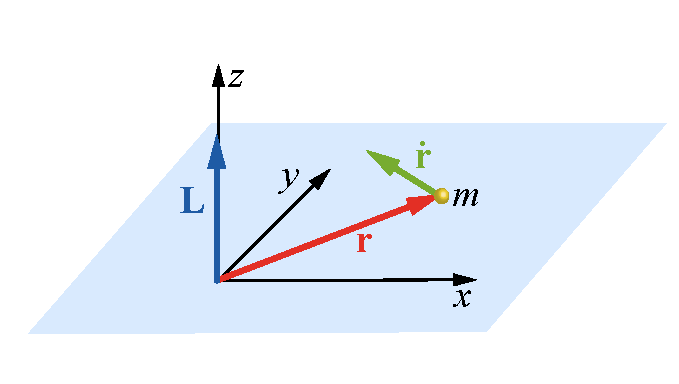
\includegraphics[width=0.5\textwidth]{Def_Drehimpuls.pdf}}
\hspace{\fill}
\rightfigure{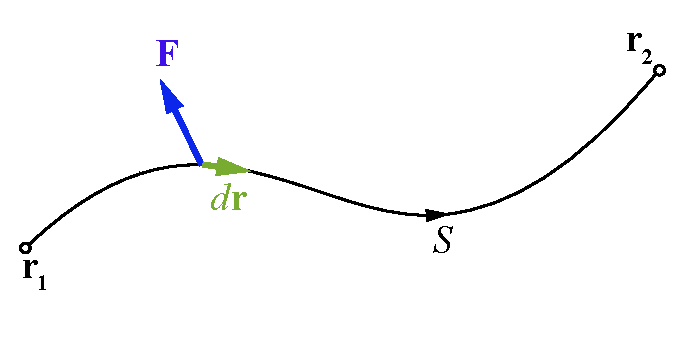
\includegraphics[width=0.5\textwidth]{Def_Arbeit.pdf}}
\leftcaption[Zur Definition des Drehimpulses eines Massepunktes.]{Zur Definition des Drehimpulses eines Massepunktes.
Im Bild wurde die Ebene, die durch die Vektoren $\vec{r}$ und $\dot{\vec{r}}$ aufgespannt wird, als $x$-$y$-Ebene gew�hlt, der Drehimpuls zeigt dann in $z$-Richtung (Rechte-Hand-Regel).}\label{abb:bew_Def_Drehimppuls}
\rightcaption[Zur Definition der Arbeit entlang eines Weges.]{Zur Definition der Arbeit entlang eines Weges $S$.}\label{abb:bew_Def_Arbeit}
\end{minipage}
\end{figure}

\subsubsection{Arbeit, Leistung und Energie}\label{kap:bew_arbeit_und_energie}

\subparagraph{\textbf{Arbeit}}\index{Arbeit}

Wir starten von der Newtonschen Bewegungsgleichung \eqref{eq:bew_NewtonBGL} und nehmen $m = \con$ an, woraus die allgemein �bliche Bewegungsgleichung 
\begin{align}
	m \ddot{\vec{r}} = \vec{F}(\vec{r},\dot{\vec{r}},t) \label{eq:bew_NewtonBGL2}
\end{align}
folgt.
Aus der Erfahrung ist bekannt, dass \anf{Arbeit} n�tig ist, um einen K�rper gegen eine Kraft zu bewegen: 
\begin{align}
	\delta W = - \vec{F} \: \mathrm{d}\vec{r} \label{eq:bew_Arbeit_infinitesimal}\,.
\end{align}
Hier ist $\delta W$ die Arbeit, die geleistet werden muss um einen Massepunkt in einem Kraftfeld $\vec{F}$ von $\vec{r}$ nach $\vec{r} + \mathrm{d}\vec{r}$ zu bewegen. 
F�r eine Bewegung entgegen der Kraft ist $ \vec{F} \cdot \D\vec{r} < 0$ und daher $\delta W > 0$, \dh es muss Arbeit aufgewendet werden, im umgekehrten Fall \anf{leistet} das Kraftfeld Arbeit.
Die gesamte geleistete Arbeit f�r eine Bewegung vom Ort $\vec{r_1}$ zum Ort $\vec{r_2}$ entlang eines Weges $S$ ist dann
\begin{align}
	W = \int\limits_{S} \delta W \mathrm{d}\vec{r} = -\int\limits_{S} \vec{F}(\vec{r},\dot{\vec{r}},t) \: \mathrm{d}\vec{r}\,.\label{eq:bew_Arbeit_total}
\end{align}
Das Integral in \eqref{eq:bew_Arbeit_total} ist ein Kurvenintegral und kann �ber eine Parametrisierung von $\vec{r}$ entlang des Weges berechnet werden, wie in \figref{bew_Def_Arbeit} dargestellt.
Dies bedeutet letztlich nichts anderes, als dass die Arbeit im Allgemeinen vom Weg abh�ngt, und dass die gr��te Arbeit wegen des Skalarproduktes in Richtung des Kraftfeldes verrichtet wird.
Kann man aber die infinitesimale Arbeit $\delta W = - \vec{F} \: \mathrm{d}\vec{r}$ als totales Differential $\mathrm{d} W $ schreiben, so gilt
\begin{align*}
	\gradv W = - \vec{F}(\vec{r})\,.
\end{align*}
Sowohl die Arbeit als auch die Kraft d�rfen dann nur vom Ort abh�ngen.
Eine solche Kraft nennt man \glslink{konservkr}{konservativ} und die entsprechende Arbeit auch potentielle Energie\index{Energie!potentielle} oder \glslink{potential}{\pot} $U$ des Kraftfeldes $\vec{F}(\vec{r})$. Man schreibt dann:
\begin{align}
	\vec{F}(\vec{r}) = -\gradv U(\vec{r}) \,.\label{eq:bew_konservative_Kraft}
\end{align}
In \probref{bew_konserv_Kraft} werden neben der Beziehung
\eqref{eq:bew_konservative_Kraft} auch einige andere Eigenschaften
des konservativen Kraftfeldes hergeleitet.

\subparagraph{\textbf{Leistung}}\index{Leistung}

Im Weiteren gehen wir von einem zeitunabh�ngigen Kraftfeld aus.
In diesem wird die geleistete Arbeit pro Zeiteinheit als Leistung definiert und kann wie folgt geschrieben werden:
\begin{align}
	P = \frac{\mathrm{d} W}{\mathrm{d}t} = - \dot{\vec{r}} \:\vec{F} = - \vec{v} \: \vec{F}\,. \label{eq:bew_Def_Leistung}
\end{align}

\subparagraph{\textbf{Energie und Energieerhaltung}}\index{Energie}\index{Energieerhaltung}

Die kinetische Energie wird definiert als
\begin{align}
	T = \frac{m}{2} \: \dot{\vec{r}}^2\,. \label{eq:bew_Def_kinEnergie}
\end{align}
Die Zeitableitung von \eqref{eq:bew_Def_kinEnergie} ergibt
	\[\frac{\mathrm{d} T}{\mathrm{d}t} = m \ddot {\vec{r}}\:\dot{\vec{r}} = \vec{F}\:\dot{\vec{r}} = - P\,.
\]
Integration �ber $t$ ergibt
	\[W_{2,1} = \int\limits_{t_1}^{t_2} \mathrm{d}t P(t)  = - \int\limits_{t_1}^{t_2} \mathrm{d}t \frac{\mathrm{d} T}{\mathrm{d}t} = T_1 -T_2\,.
\]
Die geleistete Arbeit entspricht also der �nderung der kinetischen Energie.
In einem konservativen Kraftfeld h�ngt die Arbeit nicht vom Weg ab, sondern nur von der potentiellen Energie $U$ am Anfangs- und Endpunkt, es gilt also
	\[T_1 + U_1 = T_2 + U_2\,.
\]
In einem konservativen Kraftfeld ist daher die Gesamtenergie konstant: 
\begin{align}
E = T + U = \frac{m}{2} \:\dot{\vec{r}}^2 + U(\vec{r}) = \con\,. \label{eq:bew_EnergieSatz}
\end{align}
Gleichung \eqref{eq:bew_EnergieSatz} ist der Energieerhaltungssatz der Mechanik f�r konservative Kr�fte.

\subsection{Transformation des Bezugssystems, Scheinkr�fte}\index{Scheinkraft|textbf}\index{Tr�gheitskraft|textbf}\index{Kraft!Schein-}\label{kap:bew_trafo_bezugssystem}

Physikalische Vorg�nge laufen unabh�ngig von der Wahl des KOS ab. Wir wollen Koordinatensysteme jeweils mit einem $\vec{\Sigma}$ bezeichnen.
Die Auswahl eines Bezugs- \bzw Koordinatensystems erfolgt dabei \ia so, dass sich das physikalische Problem durch m�glichst einfache Gleichungen beschreiben l�sst.

Aus dem ersten Axiom folgt die Existenz von Inertialsystemen\index{Inertialsystem}, in denen kr�ftefreie K�rper entweder ruhen oder sich mit konstanter Geschwindigkeit $\vec{v}$ bewegen.
Wir wollen nun alle denkbaren Inertialsysteme der Newtonschen Mechanik finden und auch kl�ren, wann durch den Wechsel eines Bezugssystems kein Inertialsystem mehr vorliegt.
Dabei benutzen wir der Einfachheit halber kartesische Koordinaten zu einem beliebigen Zeitpunkt $t$.
Dann kann die Umrechnung von einem Ausgangsbezugssystem $\vec{\Sigma}$ in ein anderes Bezugssystem $\vec{\Sigma}'$, in welchem wir die Koordinaten mit gestrichenen Gr��en ($\vec{r}', \vec{v}'$ usw.) beschreiben, durch eine Kombination von Translationen und Rotationen beschrieben werden. 

\subsubsection{Galilei-Transformation}\index{Transformation!Galilei-} \label{kap:bew_Galilei_Trafo}

Wir betrachten zun�chst Translationen\index{Translation} (\figref{bew_Galilei_Trafo}) und nehmen an, dass zum Zeitpunkt $t\!=\!0$ die Bezugssysteme $\vec{\Sigma}$ und $\vec{\Sigma}'$ identisch sind und keine Kr�fte wirken. 
Im Inertialsystem $\vec{\Sigma}$ gilt dann $m \ddot{\vec{r}}\! = \!0$. 
Das transformierte Bezugssystem $\vec{\Sigma}'$ geht aus dem urspr�nglichen Bezugssystem $\vec{\Sigma}$ durch eine Verschiebung $\vec{R}(t)$ hervor. 
Damit $\vec{\Sigma}'$ auch ein Inertialsystem ist, \dh der Massepunkt auch bez�glich dieses Bezugssystems ruht oder sich mit konstanter Geschwindigkeit bewegt, muss gelten $m \ddot{\vec{r}}'\! =\! 0$. 
Nach \figref{bew_Galilei_Trafo} ist aber $\vec{r} \!= \!\vec{r}' + \vec{R}(t) $, woraus folgt: $m \ddot{\vec{r}}' \!= \!m \ddot{\vec{r}} - m \ddot{\vec{R}}$. 
Dies ist nur dann gleich Null, wenn $\ddot{\vec{R}}\!=\!0$ ist, woraus folgt: $\dot{\vec{R}}\!=\!\vec{V} \!=\! \vec{const} $ und damit $\vec{R}\! = \!\vec{V} \:t$. 
Hierbei ist $\vec{V}$ die Relativgeschwindigkeit der Translation der beiden Bezugssysteme. 

\begin{figure}
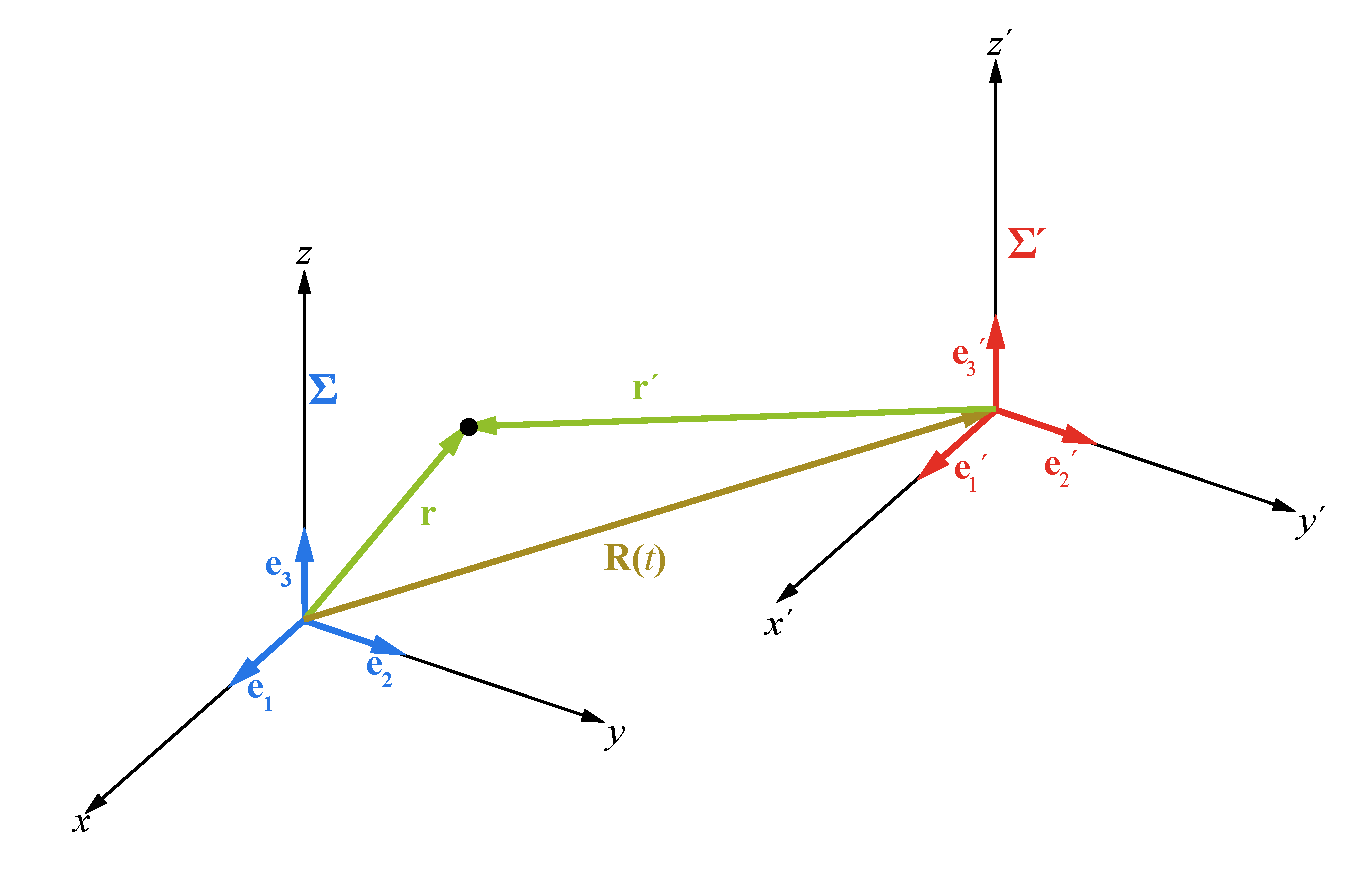
\includegraphics[width=\textwidth]{Galilei_Trafo.pdf}%
\caption[Verschiebungen zwischen Koordinatensystemen.]{Verschiebungen zwischen Koordinatensystemen. F�r die Galilei-Transformation gilt $\dot{\vec{R}}\!=\!\vec{V} \!=\! \text{const} $.}
\label{abb:bew_Galilei_Trafo}
\end{figure}

F�r die Zeit gilt in der Newtonschen Mechanik $t' = t$, sodass wir zusammenfassend formulieren k�nnen, dass man durch Translation genau dann wieder ein Inertialsystem erh�lt, wenn sich das Bezugssystem $\vec{\Sigma}'$ mit konstanter Relativgeschwindigkeit $\vec{V}$ zum Inertialsystem $\vec{\Sigma}$  bewegt.
Es gelten dann die \emph{Galilei-Transformationen}: 
\begin{align}
	\vec{r}' = \phantom'\vec{r} - \vec{V}\:t \quad \text{und} \quad t' = \phantom't\,. \label{eq:Bew_Galilei_Trafo}
\end{align}

Das zweite Newtonsche Axiom bleibt unter Galilei-Transformationen unver�ndert, die Newtonschen Bewegungsgleichungen
�ndern ihre Form beim �bergang zwischen Inertialsystemen nicht.\footnote{Selbstverst�ndlich d�rfen Inertialsysteme auch um eine beliebige Achse gegeneinander rotiert oder um einen konstanten Vektor verschoben sein. Auch darf der Zeitnullpunkt anders gew�hlt werden. Diese allgemeine Form der Galilei-Transformation ben�tigen wir hier jedoch nicht und wir beschr�nken uns daher auf die einfache Form aus Gleichung \eqref{eq:Bew_Galilei_Trafo}.}\\
Galilei-Transformationen sind die allgemeinsten Transformationen
zwischen Inertialsystemen der Newtonschen Mechanik.%
\footnote{In der relativistischen Physik l�sst man die Bedingung $t' = t$
fallen und kommt dann zu anderen Transformationen zwischen den Inertialsystemen, den sogenannten Lorentz-Transformationen.}
Wir stellen nun noch die Frage, wie die Bewegungsgleichungen in den beiden Systemen aussehen, wenn im System $\vec{\Sigma}$ eine Kraft $\vec{F} = m \ddot{\vec{r}}$ auf den Massepunkt wirkt und das System $\vec{\Sigma}'$ sich beliebig, \zb auch beschleunigt gegen�ber $\vec{\Sigma}$ bewegt.
Durch Einsetzen in die Galilei-Transformation erh�lt man $m \ddot{\vec{r}}' \!= \!m \ddot{\vec{r}}$, das zweite Axiom beh�lt also seine Form, wenn wir einfach $\vec{F} = \vec{F}'$ setzen. 
Wir m�ssen aber $\vec{F}'(\vec{r}',\dot{\vec{r}}')$ durch die transformierten Gr��en $\vec{r}',\dot{\vec{r}}'$ ausdr�cken, da die Kraft \ia von diesen Gr��en abh�ngt. 
Wir benutzen wieder $\vec{r}(t) \!= \!\vec{r}'(t) + \vec{R}(t)$, wobei diesmal $\vec{R}(t)$ beliebig zeitabh�ngig ist und erhalten
\begin{align}
	\vec{F}' \;=\; m \:\ddot{\vec{r}}' \;= \; m\: \ddot{\vec{r}} - m \ddot{\vec{R}}\;= \; \vec{F} - m \:\ddot{\vec{R}}\,.\label{eq:Bew_Galilei_Trafo_2}
\end{align}
Gleichung \eqref{eq:Bew_Galilei_Trafo_2} besagt, dass wir die Newtonsche Bewegungsgleichung auch in $\vec{\Sigma}'$ verwenden k�nnen, wenn wir zur Kraft $\vec{F}$ eine Scheinkraft\index{Scheinkraft}\index{Kraft!Schein}
$\vec{F}_\text{S} = - m \ddot{\vec{R}}$ addieren.
Scheinkr�fte sind im System $\vec{\Sigma}'$ sehr wohl real sp�r- und messbar und ergeben sich anders als die im \kap{bew_newton_axioms} beschriebenen Kr�fte nur aus der Wahl eines entsprechend bewegten Bezugssystems.\footnote{Der Begriff Scheinkraft kommt daher, dass eine solche eben f�r einen Beobachter im Inertialsystem nicht auftritt und f�r diesen somit "`scheinbar"' nicht existiert.} Wir werden im folgenden Kapitel sehen, dass auch rotierende Systeme\index{Rotation} keine Inertialsysteme mehr sind und daher in diesen ebenfalls Scheinkr�fte auftreten.


\subsubsection{Rotierende Systeme}\index{Bezugssystem!rotierendes} \index{Rotation} \label{kap:bew_rotating_systems}

\subparagraph{\textbf{Mathematische Beschreibung von Drehungen kartesischer KOS}}\index{Energie}\index{Drehung}\index{Koordinatensystem!kartesisches} \index{Drehmatrix}\index{Rotationsmatrix}

Nachdem wir zeitunabh�ngige und zeitabh�ngige Translationen von Koordinatensystemen betrachtet haben, wenden wir uns der Rotation (kartesischer) Koordinatensysteme zu, wobei wir als erstes die zeitunabh�ngige, \dh feste (Ver)Drehung zwischen zwei Koordinatensystemen betrachten wollen.
Dabei werden wir die elegante mathematische Beschreibung durch \emph{Drehmatrizen} (h�ufig auch Rotationsmatrizen genannt) kennen lernen.
Diese lassen sich herleiten, indem man ein neues gestrichenes Koordinatensystem $\vec{\Sigma}'$ aus einem (ungestrichenen) Koordinatensystem $\vec{\Sigma}$ durch Drehung um jeweils einen Winkel $\varphi$ um eine der $\vec{e}_i$-Achsen betrachtet.

\begin{figure}
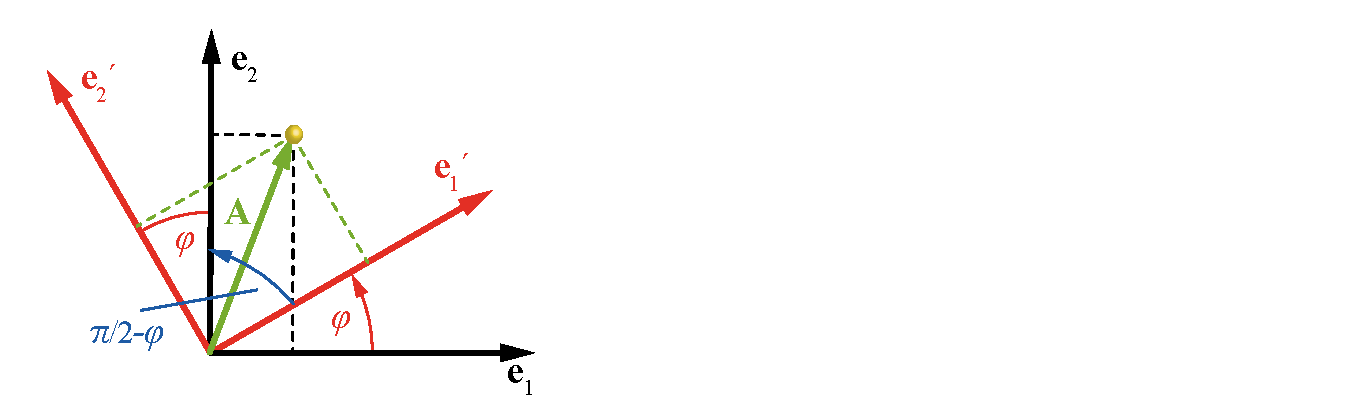
\includegraphics[width=\textwidth]{Drehmatrix.pdf}%
\caption[Zur Herleitung von Drehmatrizen.]{Zur Herleitung von Drehmatrizen. Dargestellt ist eine Drehung um die $\vec{e}_3$-Achse. Der Vektor $\vec{A}$ wird davon nicht ber�hrt, allerdings h�ngt seine Koeffizientendarstellung vom gew�hlten Koordinatensystem ab.}
\label{abb:bew_Drehmatrix}
\end{figure}

Aus \figref{bew_Drehmatrix} kann man ablesen, dass sich die $\vec{\Sigma}$-Basisvektoren zu den $\vec{\Sigma}'$-Basisvektoren folgenderma�en verhalten:\footnote{Wir bezeichnen hier die Basisvektoren allgemein mit $\vec{e}_1, \vec{e}_2, \vec{e}_3$, wobei f�r ein kartesisches \KOS $\vec{e}_1 = \veceX, \vec{e}_2 = \veceY, \vec{e}_3 = \veceZ$ gilt.}
\begin{align}
	\vec{e}_i{}' &= (\vec{e}_i{}' \cdot \vec{e}_1)\, \vec{e}_1 + (\vec{e}_i{}' \cdot \vec{e}_2)\, \vec{e}_2 = \vec{e}_i{}' = a_{i1}\,\vec{e}_1 + a_{i2}\,\vec{e}_2 \,, \label{eq:bew_Drehmatrix1_2D} 
\end{align}
\bzw verallgemeinert f�r den dreidimensionalen Fall
\begin{align}
\begin{split}
	\vec{e}_i'{} &= (\vec{e}_i{}'\cdot \vec{e}_1)\, \vec{e}_1 + (\vec{e}_i{}'\cdot \vec{e}_2)\, \vec{e}_2 + (\vec{e}_i{}'\cdot \vec{e}_3)\,\vec{e}_3\,,\\
	\vec{e}_i{}'&= a_{i1}\,\vec{e}_1 + a_{i2}\,\vec{e}_2  + a_{i3}\, \vec{e}_3\,.  
\end{split} \label{eq:bew_Drehmatrix1}
\end{align}
Die $a_{ij} = \vec{e}_i{}'\cdot \vec{e}_j$ hei�en Richtungskosinus\index{Richtungskosinus}.
F�r den Fall in \figref{bew_Drehmatrix} ergibt sich beispielsweise $\vec{e}_1{}' \cdot \vec{e}_1 = \cos \varphi\,$ und $\,\vec{e}_1{}' \cdot \vec{e}_2 = \cos {(\pi/2 - \varphi)} =
+ \sin{\varphi}\,$. Allgemein kann man die Transformation des Vektors $\vec{A}$ schreiben als:
\begin{align}
	\vec{A}' = \phantom'\mathbb{R} \: \vec{A} = \begin{pmatrix} a_{11} & a_{12} & a_{13} \\ a_{21} & a_{22} & a_{23} \\ a_{31} & a_{32} & a_{33} \end{pmatrix}\, \vec{A}\,.
\end{align}
Die Drehung um die $z$-Achse ($\vec{e}_3$) um einen positiven Winkel $\varphi$ (siehe \figref{bew_Drehmatrix}, Drehung entgegengesetzt zum Uhrzeigersinn) ist dann beispielsweise durch die Drehmatrix $\mathbb{R}_z(\varphi)$ beschrieben:
	\[\mathbb{R}_z(\varphi) \: = \;\begin{pmatrix} +\cos\varphi & +\sin\varphi & 0 \\ -\sin\varphi & +\cos\varphi & 0 \\ 0 & 0 & 1 \end{pmatrix}\,.
\]
Wir werden diese Drehmatrizen ausgiebig nutzen, insbesondere in der Himmelsmechanik und in der Mechanik starrer K�rper.

\subparagraph{\textbf{Dynamik in rotierenden Koordinatensystemen}}\index{Energie}

Wir wollen nun zeitabh�ngige Drehungen betrachten und zwei KOS $\vec{\Sigma}$ und $\vec{\Sigma}'$ gegeneinander rotieren lassen. 
Diese sollen f�r $t = 0$ �berein stimmen und f�r alle weiteren Zeiten $t$ ihren gleichen Koordinatenursprung behalten. 
Das System $\vec{\Sigma}$ sei dabei ein Inertialsystem und durch die Basis-Einheitsvektoren $\vec{e}_i$ mit $i=1\ldots3$ gegeben,
das rotierende System $\vec{\Sigma}'$ entsprechend durch die Vektoren $\vec{e}_i{}'$. 
Dabei nehmen wir an, dass nur das System $\vec{\Sigma}'$ von der Zeit abh�ngt.
Wir betrachten nun einen Vektor, der im rotierenden System $\vec{\Sigma}'$ (\figref{bew_Rot_KOS}) durch $\vec{A}'(t)$  beschrieben wird und dessen zeitliche Ver�nderung gegeben sei durch:
%\footnote{An dieser Stelle sei unterschieden zwischen dem Vektor an sich (der physikalischen Gr��e) $\vec{\mathcal{A}}$ und seiner Beschreibung $\vec{A}$ bzw. $\vec{A'}$ im jeweiligen Koordinatensystem. Eine physikalische Gr��e, z.B. $\vec{\mathcal{A}}$, muss nat�rlich immer gleich sein, unabh�ngig in welchem System man sich befindet. Im Folgenden werden wir diese Unterscheidung weglassen und einfach  $\vec{A}$ bzw. $\vec{A'}$ schreiben.}
\begin{align*}
	\frac{\D \vec{A'}}{\D t} = \frac{\D A_1'}{\D t} \:\vecpex + \frac{\D A_2'}{\D t} \:\vecpey + \frac{\D A_3'}{\D t} \:\vecpez\,.
\end{align*}
Wollen wir die zeitliche Entwicklung im Inertialsystem berechnen, m�ssen wir noch ber�cksichtigen, dass die Einheitsvektoren $\vec{e}_i$ von der Zeit abh�ngen und wir deshalb ihre zeitliche Ableitung berechnen m�ssen, also:
\begin{align*}
	\frac{\D \vec{A}}{\D t} = \frac{\D \vec{A'}}{\D t} + A_1' \: \dvecepx + A_2' \: \dvecepy + A_3' \: \dvecepz\,.
\end{align*}

\begin{figure}
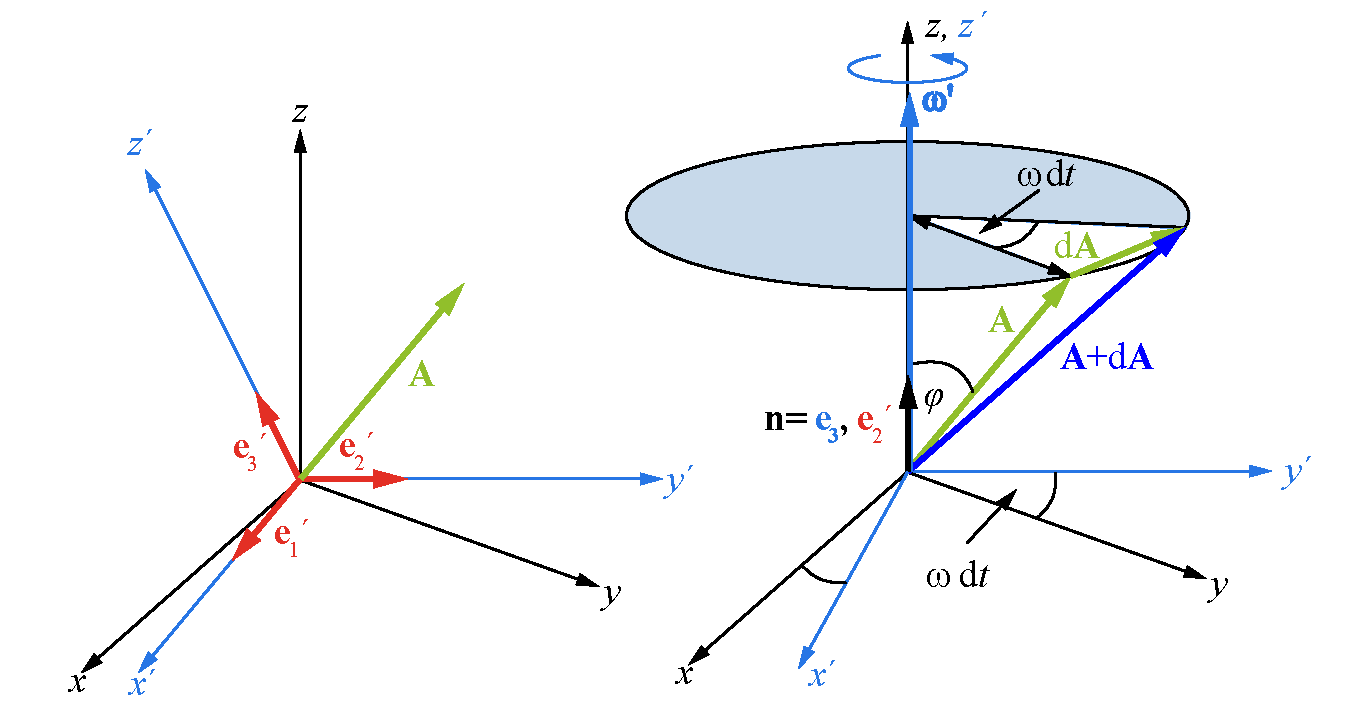
\includegraphics[width=\textwidth]{Rot_KOS.pdf}%
\caption[Rotierende Bezugssysteme.]{Rotierende Bezugssysteme. In beiden Bildern haben wir vereinfachend angenommen, dass die Nullpunkte von $\vec{\Sigma}$ und $\vec{\Sigma} '$ �bereinstimmen. Im rechten Bild nehmen wir zudem an, dass die Drehachse $\vec{n}$ sowohl mit der $z$-Achse als auch der $z'$-Achse �bereinstimmt und fest im Raum steht. $\vec{A}$ ist ein beliebiger Vektor.}%
\label{abb:bew_Rot_KOS}
\end{figure}

Wir m�ssen als n�chstes die ${\dot{\vec{e}}_i}{}'$ bestimmen, \dh herausfinden, wie sich die Einheitsvektoren ${\vec{e}_i}{}'$ aus Sicht von $\vec{\Sigma}$ �ndern.
Wir beschreiben dazu die Rotation von $\vec{\Sigma}'$ um eine Drehachse $\vec{n}$ mit dem Vektor der Winkelgeschwindigkeit $\vec{\omega}$ (\figref{bew_Rot_KOS}). 
Sowohl $\vec{n}$ als auch $\vec{\omega}$ k�nnen \ia zeitabh�ngig sein.
Unter Benutzung der Orthogonalit�tsrelationen der Einheitsvektoren ${\vec{e}_i}{}'$ findet man (in (\probref{bew_Rot_System}) im Detail ausgef�hrt) folgende Beziehung:
\begin{align}
	 A_1' \, \dvecepx + A_2' \,\dvecepy + A_3 \, \dvecepz \:&=\: \vec{\omega}' \times \vec{A}' \quad \rightarrow\ \quad 
	\frac{\mathrm{d} \vec{A}}{\D t}\: =\: \frac{\D \vec{A'}}{\D t} + \:\vec{\omega}' \times \vec{A}'\,. \label{eq:bew_Rot_System1}
\end{align}
Wir verweisen auf  \figref{bew_Rot_KOS}, in der wir den speziellen Fall dargestellt haben, bei welchem die Drehachse mit den $z$-\, und der $z'$-Achsen der beiden Koordinatensysteme zusammenf�llt. 
Wir k�nnen \eqref{eq:bew_Rot_System1} als allgemeine Transformation der Zeitableitung zwischen den beiden gegeneinander rotierenden Systemen formulieren:
\begin{align}
  % better no \mathclap here
	\underbrace{\lk \frac{\mathrm{d} \vec{A}} {\mathrm{d} t} \rk}_{\text{Ableitung in } \:\Sigma}\:
	&=\; \underbrace{\lk \frac{\mathrm{d} \vec{A}'} {\mathrm{d} t} \rk}_{\text{Ableitung in}\: \Sigma '} 
	+ \:~~\underbrace{\vec{\omega}' \times \vec{A}'}_{\text{Zusatzterm}} 
	~~=~~ \underbrace{\left\{\frac{\mathrm{d}}{\mathrm{d} t} + \vec{\omega}' \times \right\}}_{\text{Operator}} \vec{A}'~. \label{eq:bew_Rot_System2}
\end{align}
Wir weisen darauf hin, dass $\vec{\omega}'$ der Rotationsvektor ist, wie er im gestrichenen Inertialsystem $\vec{\Sigma}'$ vorliegt.
In diesem ist die Orientierung der Drehachse im Allgemeinen verschieden von der in $\vec{\Sigma}$, wie wir in \kap{bew_Coriolis-Kraft}  und den �bungen zeigen werden.\footnote{Ein Beispiel ist der Vektor der Rotationsgeschwindigkeit der Erde, der an den Polen senkrecht auf der Erdoberfl�che steht, am �quator dagegen parallel zur Erdoberfl�che.} 
Um die Transformation f�r die zweite Zeitableitung zu erhalten, wenden wir auf \eqref{eq:bew_Rot_System2} den Operator $\left\{\D / \D t  + \vec{\omega}' \times \right\}$ noch einmal an und erhalten (\probref{bew_Rot_System})
\begin{align}
	\frac{\mathrm{d^2} {\vec{A}}}{\mathrm{d} t^2} &= \frac{\mathrm{d^2} \vec{A'}}{\mathrm{d} t^2} + \:\dot{\vec{\omega}}' \times \vec{A}' + \: 2 \vec{\omega '}\times \dot{\vec{A}}'  + \:\vec{\omega'}\times( \vec{\omega '} \times \vec{A'})\,. \label{eq:bew_Rot_System3}
\end{align}
Wir k�nnen nun f�r den beliebigen Vektor $\vec{A}$ den Ortsvektor $\vec{r}$ einsetzen und erhalten
\begin{align}
	\ddot{\vec{r}} &= \ddot{\vec{r}}' + \: \dot{\vec{\omega}}' \times \vec{r'} +  \: 2 \vec{\omega}' \times \dot{\vec{r}}'  + \:\vec{\omega '}\times( \vec{\omega '} \times \vec{r'})\,. \label{eq:bew_Rot_System4}
\end{align}
Multipliziert man \eqref{eq:bew_Rot_System4} mit $m$ und fasst die Kraft $m \ddot{\vec{r}}$ im Inertialsystem $\vec{\Sigma}$ als eine externe Kraft $\vec{F}^\text{(ext)}$ auf (\zb als eine der weiter oben genannten Kr�fte wie Gravitations- oder Coulomb-Kraft), dann kann man wegen $\vec{F}^\text{(ext)} = \vec{F'}^\text{(ext)}$ die Bewegungsgleichung folgenderma�en schreiben:
\begin{align}
	\ddot{\vec{r}}' &= \frac{\vec{F}^\text{(ext)}}{m} - \: \dot{\vec{\omega}}' \times \vec{r}' - \: 2 \vec{\omega '}\times \dot{\vec{r}}'  - \:\vec{\omega}' \times( \vec{\omega}' \times \vec{r}')\,. \label{eq:bew_Rot_System5}
\end{align}
Gleichung \eqref{eq:bew_Rot_System5} ist die Erweiterung des zweiten Newtonschen Axioms auf rotierende KOS, bei denen die Ursprungskoordinaten zusammenfallen (\figref{bew_Rot_KOS}).
Wir wollen diese Beschr�nkung jetzt fallen lassen und auch eine Verschiebung $\vec{R}(t)$ des KOS zulassen.
Uns interessiert nun das Transformationsverhalten des Vektors  $\vec{r}'(t) = \vec{r}(t) - \vec{R}(t)$.
Dabei ist $\vec{r}$ der Ort des betrachteten Massepunktes relativ zum Nullpunkt in $\vec{\Sigma}$ und $\vec{r}'(t)$ derselbe Vektor vom Nullpunkt in $\vec{\Sigma} '$ aus gesehen.
Aus der zweiten Zeitableitung von $\vec{r}(t)$ nach der Bildungsvorschrift \eqref{eq:bew_Rot_System1} und \eqref{eq:bew_Rot_System3} folgt dann die Erweiterung des zweiten Newtonschen Axioms auf rotierende und linear beschleunigte Bezugssysteme:
\begin{align}
		 m \ddot{\vec{r}}' &= \vec{F}^\text{(ext)} - m \,\ddot{\vec{R}}' - m\, \dot{\vec{\omega}}' \times \lk \vec{r}' - \vec{R}' \rk - 2 m\, \vec{\omega}' \times \lk \dot{\vec{r}}' - \dot{\vec{R}}' \rk - m\, \vec{\omega}' \times \lek \vec{\omega}' \times \lk \vec{r}' - \vec{R'} \rk \rek\,, \\
		 m \ddot{\vec{r}}' &= \vec{F}^\text{(ext)} + \vec{F'}_\text{bT} + \vec{F'}_\text{bR} +\vec{F'}_\text{Cor} + \vec{F'}_\text{Z}\,.\label{eq:bew_Rot_System6}
\end{align}
Formel \eqref{eq:bew_Rot_System6} ist die Bewegungsgleichung f�r einen Massepunkt am Ort $\vec{r}'$ in einem mit $\vec{\omega}'$ rotierenden Bezugssystem $\vec{\Sigma}'$, auf den �u�ere Kr�fte $\vec{F}^\text{(ext)}$ und Scheinkr�fte wirken.
Der Verbindungsvektor $\vec{R}'$ zeigt dabei vom Ursprung des rotierenden Bezugssystems $\vec{\Sigma} '$ zum Drehzentrum.
Gleichung \eqref{eq:bew_Rot_System6} geht f�r $\vec{\omega}' = 0$ und $\ddot{\vec{R}}' = 0$ in die Form f�r Inertialsysteme �ber.
Umgekehrt wird auch ein kr�ftefreier K�rper $(\vec{F}^\text{(ext)} = 0)$ aus der Sicht eines Beobachters in einem allgemein beschleunigten und rotierenden Bezugssystem durch Scheinkr�fte beschleunigt, bleibt also nicht in Ruhe oder gleichf�rmiger Bewegung.
Alle Scheinkr�fte sind proportional zur (tr�gen) Masse und in rotierenden Systemen (mit Ausnahme von $\vec{F'}_\text{bl}$) zu $\vec{\omega}'$ \bzw $\dot{\vec{\omega}}'$.
Im Einzelnen sind das nach \eqref{eq:bew_Rot_System6}:
\begin{enumerate}
	\item Scheinkraft durch beschleunigte Translation von $\vec{\Sigma} '$ gegen�ber $\vec{\Sigma}$ (vgl. \eqref{eq:Bew_Galilei_Trafo_2}):
\begin{align} 
		\vec{F'}_\text{bT} = - m \ddot{\vec{R}}'\,. \label{eq:bew_beschl_Kraft}
\end{align}
	\item Euler-Kraft\index{Euler-Kraft}\index{Kraft!Euler-}\footnote{Leonhard Euler\indexp{Euler, Leonhard} (1707--1783) war einer der bedeutendsten Mathematiker des 18.\ Jahrhunderts. Der in der Schweiz geborene Euler, der vor allem in Berlin und St.~Petersburg forschte, war aber auch in der Physik und Astronomie t�tig und machte zahlreiche Entdeckungen in diesen Bereichen. In der Mathematik sind vor allem seine Beitr�ge zur Infinitesimalrechnung und der Graphentheorie zu nennen. In der Physik waren \ua seine Arbeiten in der Mechanik und Str�mungsdynamik wegweisend. Obwohl er bereits 1771 erblindete, war er weiterhin einer der brillantesten und produktivsten Mathematiker aller Zeiten. Eulers Arbeiten inspirierten viele Generationen von Mathematikern nachhaltig.} -- Scheinkraft durch beschleunigte Rotation von $\vec{\Sigma} '$ gegen�ber $\vec{\Sigma}$:
\begin{align} 
		\vec{F'}_\text{bR} = - m \dot{\vec{\omega}}' \times \lk \vec{r'} -\vec{R}' \rk\,. \label{eq:bew_beschl_Rotation}
\end{align}
	\item Coriolis-Kraft\index{Kraft!Coriolis-}\footnote{Gaspard Gustave de Coriolis\indexp{Coriolis, Gaspard Gustave@de Coriolis, Gaspard Gustave} (1792--1843) war ein franz�sischer Mathematiker und Physiker, der die sp�ter nach ihm benannte Coriolis-Kraft als Scheinkraft eines in einem rotierenden System bewegten K�rpers untersuchte. Au�erdem ver�ffentlichte Coriolis Arbeiten zur Wirtschaftsmathematik. Verschiedentlich wird auch Euler als Entdecker der Coriolis-Kraft genannt \cite{Grimsehl1977}.}:
\begin{align} 
		\vec{F'}_\text{Cor} = - 2 m \vec{\omega}' \times \lk \dot{\vec{r}}' - \dot{\vec{R}}' \rk\,. \label{eq:bew_Coriolis_Kraft}
\end{align}
	\item Zentrifugalkraft\index{Kraft!Zentrifugal-}:
\begin{align} 
		\vec{F'}_\text{Z} = - m \vec{\omega}' \times \lek \vec{\omega}' \times \lk \vec{r}' - \vec{R}' \rk \rek\,.\label{eq:bew_Zentrifugal_Kraft}
\end{align}
\end{enumerate} 
Wir fassen die Erkenntnisse zur Bewegung in linear beschleunigten und rotierenden Bezugssystemen zusammen:\\
Das zweite Newtonsche Axiom gilt in seiner in \eqref{eq:bew_NewtonBGL} definierten Form \emph{nur} in Inertialsystemen.
Es kann aber auch in Nichtinertialsystemen formuliert werden (Gleichungen \eqref{eq:bew_Rot_System5} und \eqref{eq:Bew_Galilei_Trafo_2}), wobei dann zus�tzliche Terme zu ber�cksichtigen sind.
Diese zus�tzlichen Terme sind die sogenannten Scheinkr�fte oder Tr�gheitskr�fte\index{Scheinkraft}\index{Tr�gheitskraft}, zu denen in rotierenden Bezugssystemen insbesondere die Zentrifugal- und die Coriolis-Kraft geh�ren.
Scheinkr�fte sind f�r einen Beobachter im mitbewegten Koordinatensystem reale Kr�fte, die allein durch die Transformation in das Nichtinertialsystem auftreten und ihren physikalischen Ursprung in der Tr�gheitskraft $m \ddot{\vec{r}}$ haben.
Das Auftreten von Scheinkr�ften ist damit immer auch ein Indiz daf�r, dass das Bezugssystem kein Inertialsystem ist. \\

%BEISPIEL 1 %%%%%%%%%%%%%%%%%%%%%%%%%%%%%%%%%%%%%%%%%%%%%%%%%%%%%%%%%%%%%%%%%%%%%%%%%%%%%%%%%%
\begin{example}{Scheinkr�fte}\\
\smallskip
An dieser Stelle wollen wir vor einem h�ufigen Fehler warnen.
Die Zentrifugalkraft $\vec{F'_\text{Z}}$ \eqref{eq:bew_Zentrifugal_Kraft} ist nicht die nach dem dritten Axiom auftretende Gegenkraft zur Radialkraft\index{Kraft!Radial-} $\vec{F}_r$ (oft auch Zentripetalkraft\index{Kraft!Zentripetal-} genannt), die einen K�rper auf eine Kreisbahn oder allgemein zur Rotation zwingt.
Das erkennt man schon daran, dass die beiden Kr�fte in unterschiedlichen Bezugssystemen definiert sind und dass sie an demselben K�rper angreifen und nicht wie im dritten Axiom gefordert an zwei verschiedenen K�rpern.
Wir wollen das an zwei Beispielen verdeutlichen:
\begin{itemize}
	\item \emph{Sitz auf einem Kettenkarusell}
	\begin{itemize}
		\item Im System $\vec{\Sigma}$: Radialkraft auf Karussellsitz (externe Kraft) und Spannung in Aufh�ngungskette (Gegenkraft)
		\item Im System $\vec{\Sigma}'$: Zentrifugalkraft auf Sitz (Scheinkraft)
	\end{itemize}
	\item \emph{Satellit in der Erdumlaufbahn}
	\begin{itemize}
		\item Im System $\vec{\Sigma}$: Gravitationskraft von Erde auf Satellit (externe Kraft) und Gravitationskraft von Satellit auf Erde (Gegenkraft)
		\item Im System $\vec{\Sigma}'$: Zentrifugalkraft (Scheinkraft)
	\end{itemize}
\end{itemize}
Die Scheinkr�fte haben keine Gegenkr�fte, die dem dritten Axiom gen�gen.
F�r die Bedingung der Ruhe bzw. gleichf�rmigen Bewegung im Bezugssystem $\vec{\Sigma} '$ kann aber sehr wohl eine Scheinkraft nach dem zweiten Newtonschen Axiom gleich einer extern wirkenden Kraft sein.
\label{bsp:Scheinkraefte}
\end{example}
%BEISPIEL %%%%%%%%%%%%%%%%%%%%%%%%%%%%%%%%%%%%%%%%%%%%%%%%%%%%%%%%%%%%%%%%%%%%%%%%%%%%%%%%%%

Wir haben das Thema der Bewegungsgleichungen in den Nichtinertialsystemen etwas ausf�hrlicher behandelt, da es in unseren �bungen eine gro�e Rolle spielen wird. 
H�ufig findet man eine unsaubere Beschreibung von solchen rotierenden Systemen durch nicht korrekte Ber�cksichtigung des jeweiligen Bezugssystems. Wir wollen daher in \kapitel{bew_anwendungen_I} und in den �bungen die Scheinkr�fte Zentrifugalkraft und Coriolis-Kraft am Beispiel der rotierenden Erde intensiv diskutieren. Zuvor aber betrachten wir noch die Mechanik von mehreren Massepunkten.

\subsection{Mechanik von Massepunktsystemen}\label{kap:bew_system_massepunkt}

\subsubsection{Schwerpunkt, Gesamtgr��en und Erhaltungss�tze}\index{Schwerpunkt} \index{Erhaltungss�tze} \label{kap:bew_basics_of_systems}

Wir erweitern das Konzept des Massepunktes auf Systeme, die aus vielen Teilchen bestehen.
Die Kr�fte, die auf jedes dieser Teilchen wirken, k�nnen zerlegt werden in
\begin{itemize}
	\item \emph{innere Kr�fte}\index{Kraft!innere}, die paarweise zwischen den Massepunkten wirken.
          Die Kraft, die $m_i$ auf $m_{\kern -1ptj}$ aus�bt, ist $\vec{F}_{\kern-2ndji}$\footnote{Hier bezeichnen $i,j$ Teilchen und keine r�umlichen Komponenten wie in \kapitel{bew_trafo_bezugssystem}.}. Nach dem dritten Axiom wirkt aber auch $\vec{F}_{\kern-1ndi\kern-1ptj}$ von $m_{\kern -1ptj}$ auf $m_i$. 
	\item \emph{�u�ere Kr�fte}\index{Kraft!�u�ere}, die von au�erhalb des betrachteten Systems auf die Massepunkte wirken.
          Auf den Massepunkt $m_i$ wirkt eine Kraft (\bzw Beschleunigung) $\vec{F}^\text{(ext)}_{i}$.
          Wirken keine �u�eren Kr�fte auf das System, so nennt man das System \emph{isoliert}\index{System!isoliertes}.
\end{itemize}
Wir definieren nun: 
\begin{align}
	&\text{Gesamtmasse} &M &= m_\text{ges} = \sum\nolimits_{i} m_i\,, \\
        &\text{\gls{com}}&\vec{R}_S &= (1/M)\,\sum\nolimits_{i} m_i \vec{r}_i\,,\\
	&\text{�u�ere Gesamtkraft}&\vec{F}^\text{\,(ext)} &= \sum\nolimits_{i} \vec{F}^\text{\,(ext)}_i\,, \\ 
	&\text{Gesamtimpuls}&\vec{p} &= \sum\nolimits_{i} \vec{p}_i = \sum\nolimits_{i} m_i \dot{\vec{r}}_i\,, \\ 
	&\text{�u�eres Gesamtdrehmoment}&\vec{M}_\text{D}^\text{\,(ext)} &= \sum\nolimits_{i} \vec{M}_{\text{D}\,i}^\text{\,(ext)} = \sum\nolimits_{i} \vec{r}_i \times \vec{F}^\text{\,(ext)}_i\,, \\ 
	&\text{Gesamtdrehimpuls} &\vec{L} &= \sum\nolimits_{i} \vec{L}_i = \sum\nolimits_{i} m_i \vec{r}_i \times \dot{\vec{r}}_i\,. \label{eq:bew_Gesamtgroessen}
\end{align}
Offensichtlich sind diese Beziehungen vom Bezugssystem abh�ngig.
Unter Benutzung des dritten Axioms f�r die Kr�fte $\vec{F}_{ij}$ zwischen den Teilchen kann man zeigen, dass folgender Schwerpunktsatz gilt:
\begin{align}
	M \ddot{\vec{R}}_S &= \vec{F}^\text{\,(ext)}\,.\label{eq:bew_Schwerpunkt_Satz}
\end{align}
Der Schwerpunkt bewegt sich also wie ein einzelner Massepunkt mit der Gesamtmasse $M$ unter dem Einfluss aller \anf{externen} Kr�fte.
Oder allgemeiner:
\begin{align}
	\dot{\vec{p}} &= \vec{F}^\text{\,(ext)}\,,\label{eq:bew_Schwerpunkt_Satz2} 
\end{align}
woraus man f�r $\vec{F}^\text{\,(ext)} = 0$ den \emph{Gesamtimpulserhaltungssatz}\index{Impulserhaltungssatz} erh�lt:
\begin{align}
	\vec{F}^\text{\,(ext)} = 0 \quad \Leftrightarrow \quad \vec{p} = \con\,.\label{eq:bew_Ges_Impulserhaltung} 
\end{align}
Der Gesamtimpuls ist also genau dann erhalten, wenn die �u�ere Gesamtkraft verschwindet, wobei die einzelnen Kr�fte $\vec{F}^\text{(ext)}_{i}$ und $\vec{F}_{ij}$ nicht verschwinden m�ssen.
Ebenso sind die einzelnen Impulse $\vec{p}_i$ \ia nicht erhalten. 

Analog findet man f�r die zeitliche Ableitung des Gesamtdrehimpulses ${\vec{L}}$ f�r den Fall, dass die inneren Kr�fte auf die einzelnen Teilchen Zentralkr�fte sind und das �u�ere Drehmoment verschwindet (\probref{bew_VielteilchenI}), den \emph{Gesamtdrehimpulserhaltungssatz}\index{Drehimpulserhaltungssatz}:
\begin{align}
	\vec{M}_\text{D}^\text{\,(ext)} = 0 \quad \Leftrightarrow \quad \vec{L} = \con\,.\label{eq:bew_Ges_Drehimpulserhaltung} 
\end{align}

Definiert man weiter: \index{Kraft!dissipative}
\begin{align}
	&\text{Kinetische Energie des Systems} &T&= \frac{1}{2}\sum\nolimits_{i} m_i\dot{\vec{r}}_i \cdot \dot{\vec{r}}_i\,, \\
	&\text{Konservativer Anteil der externen Kr�fte} &\vec{F}^\text{\,(kons)}_i&= - \frac{\partial U}{\partial \vec{r}_i}\,, \\
        &\text{\glslink{disskr}{Dissipativer Anteil der externen Kr�fte}} &\vec{F}^\text{\,(diss)}_i&= \vec{F}^\text{\,(ext)}_i - \vec{F}^\text{\,(kons)}_i = \vec{F}^\text{\,(ext)}_i + \frac{\partial U}{\partial \vec{r}_i}\,, \\
	&\text{Gesamtenergie des Systems} &E&= T + U\,, \label{eq:bew_Ges_Energie}
\end{align}
so erh�lt man den \emph{Energieerhaltungssatz}\index{Energieerhaltungssatz} f�r das konservative System\index{System!konservatives}, im Fall eines nicht-konservativen Systems erh�lt man den Energieverlust:
\begin{align}
	\text{Konservatives System:} \quad & \forall i\,\vec{F}^\text{\,(diss)}_i = 0 \quad \Longleftrightarrow \quad E = T + U = \con\,, \nonumber \\
	\text{Nicht-konservatives System:} \quad & \frac{\mathrm{d}}{\mathrm{d} t} E = \frac{\mathrm{d}}{\mathrm{d} t} \lk T + U \rk  = \sum\nolimits_{i} \vec{F}^\text{\,(diss)}_i \cdot \dot{\vec{r}}_i\,. \label{eq:bew_Ges_Energieerhaltung} 
\end{align}\

Da die kinetische Energie eine Funktion der Geschwindigkeit des Massepunktes ist, h�ngt sie von dem Bezugssystems ab.
Allgemein gilt, dass die kinetische Energie in einem beliebigen Bezugssystem die Summe der kinetischen Energie der im Schwerpunkt konzentrierten Gesamtmasse und der kinetischen Energie der Massepunkte im Schwerpunktsystem ist.
Als \gls{comsys} (im Englischen auch oft als \textit{Center-of-Mass System CoMS} geschrieben)\index{Schwerpunktsystem}\index{Center-of-mass System (CoS)}  wird ein Bezugssystem definiert, in dem der Koordinatenursprung in den Schwerpunkt des physikalischen Systems gelegt wird.
Das Schwerpunktsystem ist sehr vorteilhaft zur Beschreibung vieler dynamische Vorg�nge wie \zb von Sto�- und Streuprozessen.
Aus der Definition des Schwerpunktsystems folgt direkt, dass in ihm der Gesamtimpuls der beteiligten Massen zu jeder Zeit, vor wie nach einem Sto�- oder Reaktionsvorgang, gleich Null ist.
Mit den genannten Erhaltungss�tzen\index{Erhaltungss�tze} lassen sich viele Probleme sehr elegant l�sen.
Wir geben zun�chst noch eine kurze Einf�hrung in den einfachsten, aber zugleich sehr wichtigen Spezialfall der Vielteilchensysteme, in das \emph{Zweik�rperproblem} (ZKP)\index{Zweik�rperproblem}.
Wir werden das ZKP speziell f�r Zentralkraftfelder ausgiebig in der Himmelsmechanik (Band II, Kapitel 3) und der Astrodynamik (Band II, Kapitel 4) behandeln. 
Im Folgenden werden wir uns deswegen nur auf die wesentlichen Punkte konzentrieren und ansonsten
auf die entsprechenden Kapitel verweisen.\\
Im weiteren Verlauf dieses Kapitels werden wir uns besonders auf Zweik�rperprobleme, bei denen ein oder mehrere Teilchen zumindest zeitweise ungebunden sind konzentrieren.
Solche Prozesse werden \ia als Streu- oder Sto�prozesse bezeichnet.

\subsubsection{Zweik�rperproblem -- effektives Eink�rperproblem}\index{Zweik�rperproblem} \index{Eink�rperproblem!effektives} \label{kap:bew_ZKP_EEKP}

Das Zweik�rperproblem kann in vielen F�llen vereinfacht und auf ein sogenanntes \emph{effektives} Eink�rperproblem zur�ckgef�hrt werden.
Dies gilt besonders f�r die Bewegung in einem Zentralkraftfeld $\vec{F}(\vec{r}) = F(r) \vec{r}/r = -\gradv U(r)$.
F�hrt man n�mlich anstelle der Massen $m_1$ und $m_2$ die \emph{reduzierte} oder auch als \emph{effektive} Masse bezeichnete \index{Masse!reduzierte} 
\begin{align}
	m_\text{eff} = \frac{m_1 m_2}{m_1 + m_2}  \label{eq:bew_red_Masse}
\end{align}
ein, dann vereinfachen sich die Bewegungsgleichungen f�r die beiden Massepunkte zu einer Bewegungsgleichung f�r einen einzelnen Massepunkt mit der reduzierten Masse in einem �u�eren \potz{} $U(r)$:
\begin{align}
	m_\text{eff} \ddot{\vec{r}} = -\gradv U(r)\,. \label{eq:bew_eff_EKP}
\end{align}
Sind die beiden Massen ($m_i = m$) identisch, ist $m_\text{eff}  = m/2$ und der Schwerpunkt liegt in der Mitte zwischen den Massen.
Auch der Fall $m_2=m \ll  m_1=M$, bei dem sich in guter N�herung die Masse $m$ um eine quasi ruhende Masse $M$ bewegt, ist in der Himmelsmechanik genau wie in vielen anderen Bereichen der Physik von Bedeutung.

\subsubsection{Zweik�rperproblem im Zentralkraftfeld $U(r)$}  \label{kap:bew_ZKP_NZKF}

Dieser wichtige Spezialfall wird ausf�hrlich in der Himmelsmechanik (Band II, Kapitel 3) diskutiert. 
Dort wollen wir auch die L�sung der Bewegungsgleichungen des sogenannten Kepler-Problems\index{Keplerproblem}\indexp{Kepler, Johannes}\footnote{Johannes Kepler (1571 -- 1630 ) war ein deutscher Astronom und Physiker. Er entdeckte die Gesetzm��igkeiten, nach denen sich Planeten um die Sonne bewegen. Seine Formulierung der drei Planetengesetze machten aus dem mittelalterlichen Weltbild ein dynamisches System, in dem die Sonne durch ihre Fernwirkung die Planeten aktiv beeinflusst.} behandeln, womit wir Planetenbahnen und Bahnen anderer Himmelsk�rper beschreiben k�nnen.
Hierbei wird das zentrale Kraftfeld mit dem \pot{} $U(r) = -\kappa / r$ modelliert.
Wir werden aber schon hier in diesem Abschnitt einige allgemeine Aussagen zum Zweik�rperproblem im Zentralkraftfeld herleiten; vor allem f�r ungebundene Zust�nde, die von entscheidender Bedeutung f�r viele Bereiche der Physik sind.
Im Kapitel Streuprozesse (\ref{kap:bew_stoss}) werden wir diese dann bereits sehr vorteilhaft anwenden k�nnen.
In \figref{bew_ZKF_Beispiele} sind verschiedene in der Physik h�ufig vorkommende Zentralkraft\potsuf{}e charakterisiert. Darunter sind die Newtonsche
Gravitation, die Coulomb-Kraft gleichnamiger Ladungen, die Kernkraft
(aus dem Yukawa\footnote{Hideki Yukawa (1907--1981) war der erste japanische Physiker, der 1949 den Nobelpreis f�r seine Vorhersage der Existenz der Mesonen erhielt. Die Mesonen bilden die Grundlage der Theorie der starken Kernkr�fte.}-Potential) und eine quadratische Federkraft. 

\begin{figure}
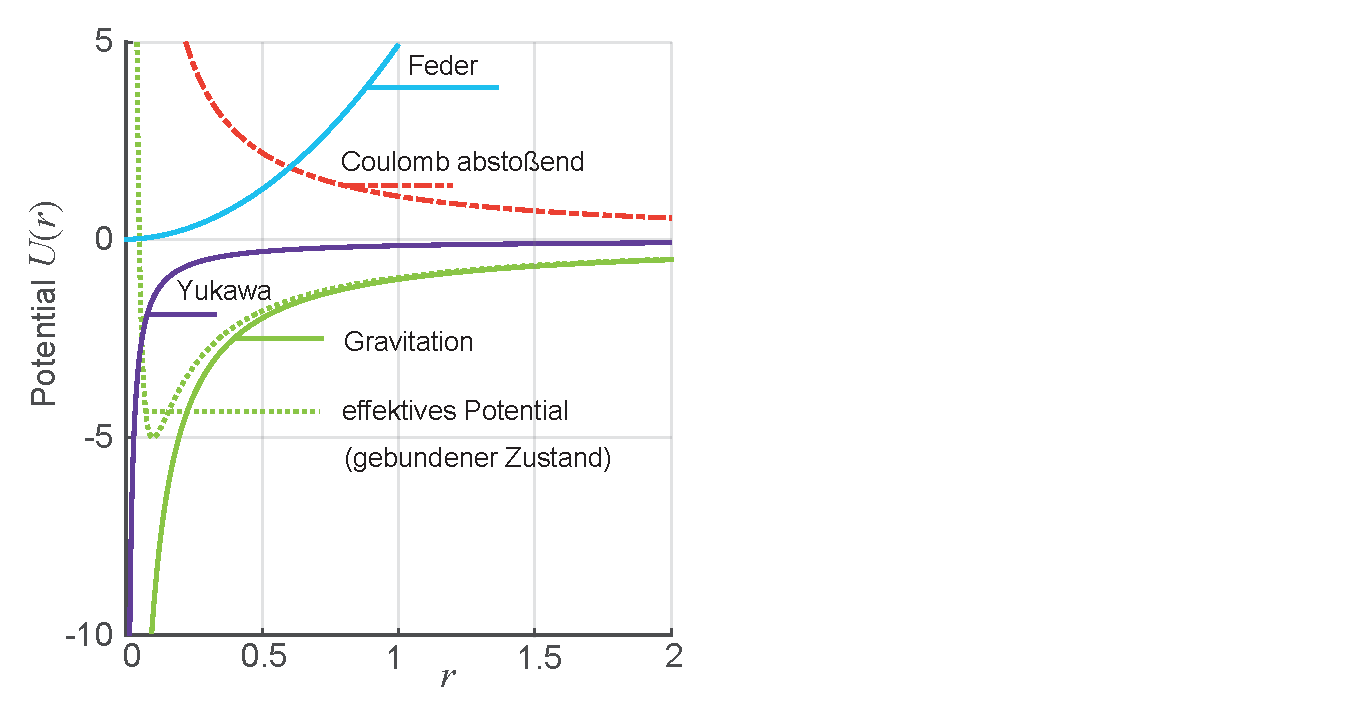
\includegraphics[width=\textwidth]{ZKF_Beispiele.pdf}
\caption[Beispiele f�r \pot{}e verschiedener Zentralkraftfelder.] {Beispiele f�r \pot{}e verschiedener Zentralkraftfelder: Newtonsche Gravitation, Coulomb-Kraft (sich absto�ende Ladungen), Kernkraft (aus Yukawa\indexp{Yukawa, Hideki}-\pot) und Federkraft. Ebenfalls gezeigt ist das effektive \pot{} $U_\text{eff}$ \eqref{eq:bew_Eff_Potential} f�r die Gravitation unter Ber�cksichtigung des Drehimpulses. F�r die anderen \pot{}e (Ausnahme: Coulomb-Potential bei sich absto�enden Ladungen) gibt es ebenfalls effektive \pot{}e und damit die M�glichkeit gebundener Zust�nde.}
\label{abb:bew_ZKF_Beispiele}
\end{figure}


\subparagraph{\textbf{Drehimpuls und Energieerhaltung, effektives \pot}}

Wir k�nnen uns das L�sen der Bewegungsgleichung \eqref{eq:bew_eff_EKP} vereinfachen, indem wir die Erhaltungss�tze ausnutzen. 
Daher wollen wir als erstes Erhaltungsgr��en identifizieren%
\footnote{H�ufig, besonders auch in der Himmelsmechanik,
werden Erhaltungsgr��en auch Bewegungsintegrale genannt,
da das Identifizieren einer Erhaltungsgr��e einer einmaligen
Integration der Bewegungsgleichung entspricht.}.

Der Drehimpulserhaltungssatz \eqref{eq:bew_Ges_Drehimpulserhaltung} kann f�r das allgemeine Zentralkraft\potsuf{} in ebenen Polarkoordinaten geschrieben werden als 
\begin{align}
  \left|\vec{L}\right| = m_\text{eff}\: \left|\vec{r} \times \dot{\vec{r}} \right| = L = \text{const} =   m_\text{eff}\: r^2 \dot{\varphi}\,. \label{eq:bew_Drehimp_polar}
\end{align}
Der Energieerhaltungssatz \eqref{eq:bew_Ges_Energieerhaltung} in diesen Koordinaten lautet:
\begin{align}
  E &= T + U = \text{const} = \frac{1}{2}  m_\text{eff}\: \dot{\vec{r}}^2 + U(r) =  \frac{1}{2}  m_\text{eff}\: \dot{r}^2 + \frac{L^2}{2  m_\text{eff}\: r^2} + U(r)\,, \label{eq:bew_Energie_polar}
\end{align}
womit wir durch
\begin{align}
	U_\text{eff}(r) &= U(r) + \frac{L^2}{2  m_\text{eff}\: r^2} \label{eq:bew_Eff_Potential}
\end{align}
das sogenannte \emph{effektive \pot}\index{Potential!effektives} definieren, in welchem sich (mathematisch gesehen) die effektive Masse $m_\text{eff}$ bewegt.
Mit diesen beiden Erhaltungss�tzen wollen wir das Zweik�rperproblem im Zentralkraftfeld l�sen.

\subparagraph{\textbf{Bahnkurven im Newtonschen Zentralkraftfeld  $U(r)= -\kappa/r$}}

Oft ist man gar nicht an der zeitlichen Entwicklung der Bewegung, sondern nur an der r�umlichen Form der Bahn interessiert.
Man kann daran \zb erkennen, ob die Bahn geschlossen, gebunden ($r$ bleibt endlich) oder ungebunden ($r$ divergiert) ist.
Wiederum unter Verwendung ebener Polarkoordinaten l�sst sich die Bahnkurve mit \eqref{eq:bew_Energie_polar} �ber
\begin{align}
	\frac{\mathrm{d}r}{\mathrm{d}\varphi} = \frac{\mathrm{d}r}{\mathrm{d}t} \frac{\mathrm{d}t}{\mathrm{d}\varphi} = \frac{\dot{r}}{\dot{\varphi}} = \frac{\sqrt{2 \lk E - U_\text{eff}(r) \rk/ m_\text{eff}\:}}{L/\lk m_\text{eff} r^2 \rk}
\end{align}
aus dem \pot{} $U_\text{eff}(r)$ berechnen.
Hierbei ergibt sich der Z�hler aus dem Energieerhaltungssatz, der Nenner aus dem Drehimpulserhaltungssatz.
Wir haben also aus den beiden Erhaltungss�tzen
eine Differentialgleichung f�r die Bahnform erhalten,
die man bei bekanntem effektiven \potz{} l�sen kann,
wodurch man die Bahnkurve
\begin{align}
\varphi(r) - \varphi_0 &=  L \int\limits_{r_0}^{r} \frac{\D r'}{r'^2 \sqrt{2  m_\text{eff}\: \lk  E - U_\text{eff}(r') \rk}} 
= L \int\limits_{r_0}^{r} \frac{\D r'}{r'^2 \sqrt{2  m_\text{eff}\: \lk E + \kappa/r' - L^2/(2  m_\text{eff}\,r'^2) \rk}}~, \label{eq:bew_Bahn_implizit1}
\end{align}
\bzw mit $r'=1/q'$
\begin{align}
\varphi(q) - \varphi_0 &= - L \int\limits_{q_0}^{q} \frac{\D q'}{\sqrt{2  m_\text{eff}\, E + 2  m_\text{eff}\,\kappa  q' - L^2\,  +-q'^2}} \label{eq:bew_Bahn_implizit2}
\end{align}
erh�lt.
Die in \eqref{eq:bew_Bahn_implizit1} und \eqref{eq:bew_Bahn_implizit2} auftretende Energie $E$ und der konstante Drehimpuls $L$ bilden zusammen mit den Anfangsbedingungen die Integrationskonstanten und legen damit die Form der Bahnkurve eindeutig fest. 
Die Bahn ist also durch das effektive \potz{} und die physikalischen Erhaltungsgr��en Energie $E$ und Drehimpuls $L$ bestimmt, welche man in zwei konstante, wie wir sehen werden geometrische Parameter �berf�hren kann.
Diese sind die (numerische) \glslink{exzentr}{\emph{Exzentrizit�t}} $\epsilon$ und der \emph{\gls{bahnpar}} $p$: 
\begin{align}
                \epsilon &= \sqrt{\frac{2 L^2 E}{ m_\text{eff}\: \kappa^2} + 1} ~~ ( \geq 0)\text{ und} \label{eq:bew_Bahn_Exzentrizitaet} 
\end{align}
\begin{align}
		p &= \frac{ L^2}{ m_\text{eff}\: \kappa}\,. 	\label{eq:bew_Bahn_Parameter} 
\end{align}
Mit diesen Parametern kann man \eqref{eq:bew_Bahn_implizit2} integrieren (siehe \cite{Gradshteyn1980}) und erh�lt die allgemeine Bahnkurve im Newtonschen Gravitations\potsuf{} 
\begin{align}
	  r(\varphi) = \frac{p}{1+\epsilon \cos{(\varphi - \varphi_0)}}\,. \label{eq:bew_Bahn_explizit}
\end{align}

Man kann nun abh�ngig vom Parameter $\epsilon$ drei F�lle unterscheiden:
\begin{itemize}
	\item \emph{Ellipsenbahnen f�r} $\epsilon < 1$

F�r $\epsilon < 1$ ergibt \eqref{eq:bew_Bahn_explizit} eine Ellipsenbahn (\figref{bew_Ellipse_Hyperbel}a).
Dies kann man zeigen, indem man mit den geometrischen Parametern der Ellipse $a$ (gro�e Halbachse) und $b=a \sqrt{1-\epsilon^2} $ (kleine Halbachse) und dem Bahnparameter $p= a (1-\epsilon^2)$ die Erf�llung der Ellipsengleichung zeigt.
Der Fall $\epsilon=0$ entspricht dem Spezialfall der Kreisbahn.

\begin{figure}
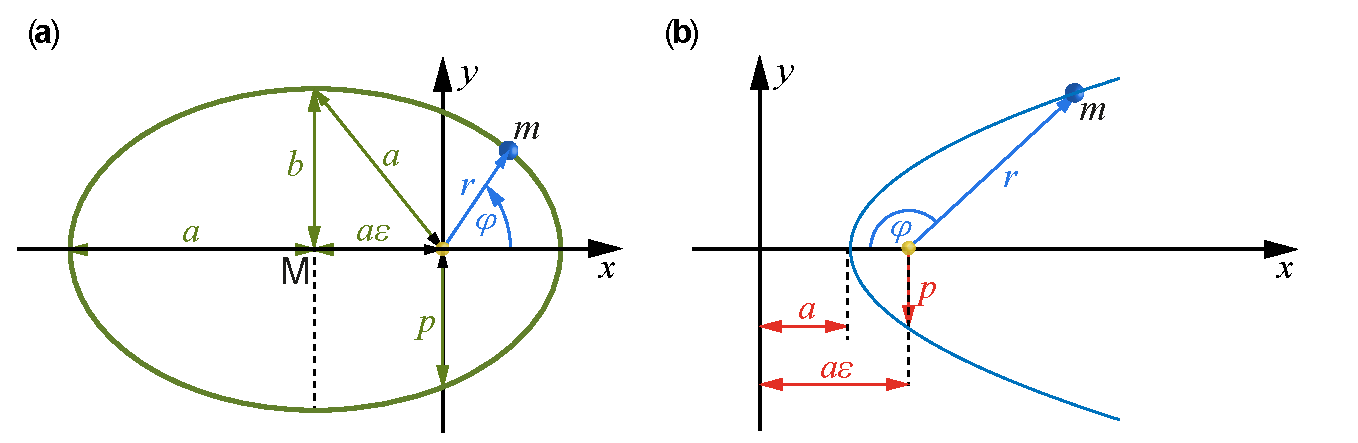
\includegraphics[width=\textwidth]{Ellipse_Hyperbel.pdf}
\caption[Geometrie von Ellipse und Hyperbel.] {Geometrie von \fa Ellipse und \fb Hyperbel.}
\label{abb:bew_Ellipse_Hyperbel}
\end{figure}

Im Newtonschen Gravitations\potsuf{} \eqref{eq:bew_Gravitationskraft} ist $\kappa > 0$, woraus wegen \eqref{eq:bew_Bahn_Exzentrizitaet} f�r $\epsilon < 1$ sofort $E <0$ folgt.
Bahnen k�nnen im $1/r$-\pot{} also nur dann gebunden sein, wenn $E < 0$ gilt.
Man sieht das auch an \eqref{eq:bew_Bahn_explizit}, wo wegen $\epsilon < 1$ der Nenner $ 1+ \epsilon\cos{\varphi}$ stets positiv und $r$ damit endlich ist.\\

\item \emph{Hyperbelbahnen f�r} $\epsilon > 1$

Der Fall $\epsilon > 1$ f�hrt wegen \eqref{eq:bew_Bahn_Exzentrizitaet} zwingend auf $E > 0$.
Gleichung \eqref{eq:bew_Bahn_explizit} beschreibt dann einen der beiden �ste einer Hyperbel (\figref{bew_Ellipse_Hyperbel}b).
Der Abstand $r$ wird unendlich, wenn $\:1 + \epsilon \cos{(\varphi -\varphi_0)}$ gegen Null strebt.
Die Bahn ist dann eingeschr�nkt auf
\begin{align}
	\left| \varphi \right| \: &\leq \varphi_\infty = \arccos \lk -\frac{1}{\epsilon} \rk \leq \frac{\pi}{2} \; , \nonumber \\
	r_\text{min} &= \frac{p}{1+\epsilon} \leq r \: \leq \infty\;.\label{eq:bew_hyp_asymptote}
\end{align}
Diese Art der Bewegung mit einem eingeschr�nkten Winkelbereich f�r $\varphi$ nennt man \emph{Streuung}\index{Streuung} (\figref{bew_Streuwinkel}).
Der Massepunkt kommt aus dem Unendlichen, wechselwirkt im \pot{} und l�uft anschlie�end unter einem \emph{Streuwinkel}\index{Streuwinkel} wieder ins Unendliche.
Wir werden im n�chsten Kapitel diese Streuprozesse genauer untersuchen.
Wir weisen hier explizit darauf hin, dass Hyperbelbahnen nicht nur durch anziehende \pot{}kr�fte wie die Newtonsche Gravitation entstehen k�nnen, sondern auch durch absto�ende \pot{}e wie sie durch gleichartige Ladungen hervorgerufen werden.
Man erkennt aus \eqref{eq:bew_Bahn_Exzentrizitaet}, dass die Exzentrizit�t $\epsilon$ der Bahn unabh�ngig vom Vorzeichen von $\kappa$ ist, der Bahnparameter $p$ wird bei $\kappa < 0$ jedoch negativ.
Da f�r den Abstand immer $r \geq 0$ gilt, muss der Nenner von \eqref{eq:bew_Bahn_explizit} insgesamt negativ werden, was nur f�r $\epsilon > 1$ und damit $ E > 0$ erf�llt werden kann.
F�r absto�ende Zentralkraft\potsuf{}e existieren damit keine gebundenen Bahnen. \\

\item \emph{Parabelbahnen f�r} $\epsilon = 1$

F�r $\epsilon = 1$ folgt aus \eqref{eq:bew_Bahn_explizit} der Spezialfall einer Parabelbahn.
Wir wollen diese hier nicht weiter behandeln, da man \zb in der Himmelsmechanik in der Regel Ellipsenbahnen bei gebundenen und Hyperbelbahnen bei ungebundenen Himmelsk�rpern beobachtet. 
\end{itemize}
Wir haben hier nur einen kurzen Abriss der Physik der Bewegung im Zentralkraftfeld gegeben, der uns aber erlaubt, eine Reihe von Problemen und �bungen zu l�sen (siehe \zb \probref{bew_SwingBy}).
Im Kapitel Himmelsmechanik (Band II, Kapitel 3) werden wir
die Bewegungen auch in ihrer Zeitabh�ngigkeit berechnen
und zudem Abweichungen von diesen einfachen Bahnen detailliert
untersuchen.
Wir werden dort auch eine leicht andere (\zt durch historische Konventionen bedingte) Notation verwenden und mit sogenannten spezifischen, \dh auf die Masse des bewegten K�rpers bezogenen Gr��en rechnen.

\subsubsection{Sto�- und Streuprozesse}\index{Sto�} \index{Streuung|textbf} \label{kap:bew_stoss}

\subparagraph{\textbf{Bezugssystem bei Streuung}} \index{Schwerpunktsystem}

Wir wollen uns nun den Sto�- und Streuprozessen\footnote{Sto� und Streuung werden h�ufig synonym gebraucht.
Unter Streuung verstehen wir die �nderung der Bewegung eines Teilchens/K�rpers durch Wechselwirkung mit einem anderen Teilchen/K�rper.
Sto� bezeichnet hingegen den speziellen Fall, dass sich die beiden Teilchen/K�rper bei dieser Wechselwirkung ber�hren, was nat�rlich bei St��en von Massepunkten nur ein theoretisches Konzept (wie der Massepunkt selbst), bei ausgedehnten K�rpern aber sehr wohl von Bedeutung ist.} zweier Massepunkte zuwenden.
Wir haben gesehen, dass bei der Streuung die einfallenden Teilchen um den sogenannten Streuwinkel\index{Streuwinkel} $\vartheta$ abgelenkt werden.
Wir werden jetzt zeigen, dass sich $\vartheta$ aus dem Wechselwirkungs\potsuf{} \index{Potential!Wechselwirkungspotential} berechnen l�sst.
Daher lassen sich aus der experimentellen Bestimmung von Streuwinkeln und des damit zusammenh�ngenden (noch zu definierenden)  Wirkungsquerschnitts R�ckschl�sse �ber die Art und Gr��e der Wechselwirkung ziehen.
Bei der Behandlung der Streuprozesse wollen wir zwei Bezugssysteme verwenden:

\begin{enumerate}
	\item das Laborsystem $\vec{\Sigma}_\text{L}$, in dem das Experiment beobachtet und beschrieben wird und die Koordinaten ungestrichen (\zb $x$) gekennzeichnet sind, und 
	\item das Schwerpunktsystem $\vec{\Sigma}_\text{S}$, in welchem der Schwerpunkt des Systems im Ursprung ruht und die Koordinaten gestrichen (\zb $x'$) sind. 
\end{enumerate}

\subparagraph{\textbf{Elastische Streuung zwischen zwei Teilchen}}\index{Streuung!elastische}

\begin{figure}
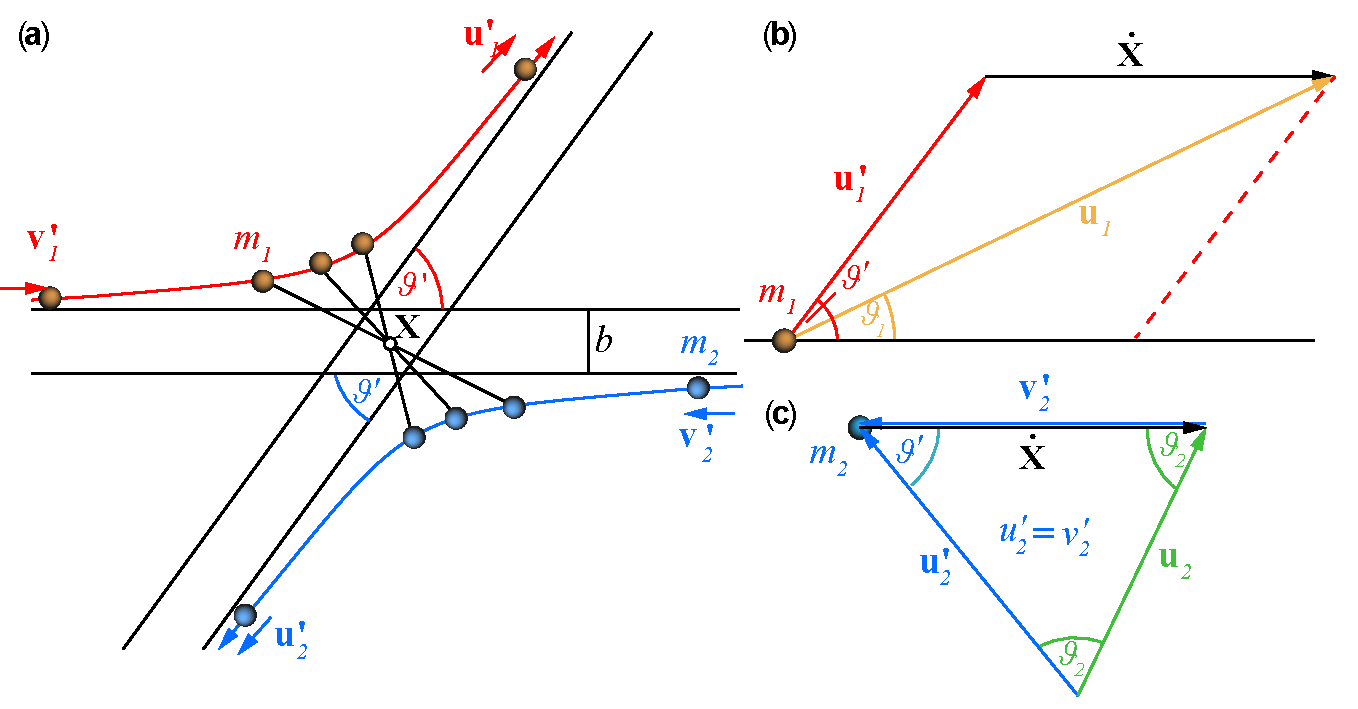
\includegraphics[width=\textwidth]{Streuwinkel.pdf}
\caption[Streuwinkel im Schwerpunktsystem und im Laborsystem.] {\fa Streuwinkel $\vartheta'$ im Schwerpunktsystem $\vec{\Sigma}_\text{S}$ f�r zwei gleiche Massen $m_1 = m_2$. Dargestellt sind auch die Asymptoten ins Unendliche und der asymptotische Abstand $b$, der Sto�parameter genannt wird. \fb Beziehung zwischen den Streuwinkeln $\vartheta'$ in $\vec{\Sigma}_\text{S}$ und $\vartheta_1$ des bewegten Teilchens $m_2$ im Laborsystem $\vec{\Sigma}_\text{L}$. Die Masse $m_2$ ruht vor dem Sto� in $\vec{\Sigma}_\text{L}$. \fc Beziehung zwischen dem Streuwinkel $\vartheta'$ f�r die bewegte Masse $m_1$ in $\vec{\Sigma}_\text{S}$ und dem Winkel $\vartheta_2$ des anfangs ruhenden Teilchens $m_2$ im Laborsystem $\vec{\Sigma}_\text{L}$ (nach \cite{Bartelmann2015}).}
\label{abb:bew_Streuwinkel}
\end{figure}

Wir wollen uns auf elastische Wechselwirkungen beschr�nken, die noch dazu im Unendlichen verschwinden.
Dabei bleibt die mechanische Energie, \dh die Summe aus kinetischer und potenzieller Energie, erhalten.
Neben dem Energieerhaltungssatz gilt auch der Impulserhaltungssatz, wobei wir annehmen, dass sich die Massen der wechselwirkenden Teilchen nicht �ndern.
Wir betrachten  die Massen $m_1$ und $m_2$ mit den Geschwindigkeiten $\vec{v}_1$ und $\vec{v}_2$ vor dem Sto� und $\vec{u}_1$ und $\vec{u}_2$ nach dem Sto�.
Dann gelten im Unendlichen (wo das \pot{} verschwindet) 
\begin{align}
	\text{Impulserhaltung:} \qquad &m_1 \,\vec{v}_1 + m_2\, \vec{v}_2 = m_1 \,\vec{u}_1 + m_2 \,\vec{u}_2   \label{eq:bew_Streuung1} \\ 
	\text{und Energieerhaltung:} \qquad &\frac{m_1}{2}\, \vec{v}_1^2 + \frac{m_2}{2} \, \vec{v}_2^2 = \frac{m_1}{2} \,\vec{u}_1^2 +\frac{m_2}{2}\, \vec{u}_2^2\,. \label{eq:bew_Streuung2}
\end{align}
Die entsprechenden Erhaltungss�tze lauten im Schwerpunktsystem folglich
\begin{align}
	m_1 \,\vec{v'}_1 + m_2 \,\vec{v'}_2 &= m_1\,\vec{u'}_1 + m_2 \,\vec{u'}_2 = 0 \qquad \text{und} \label{eq:bew_Streuung1a} \\ 
	\frac{m_1}{2} \,\vec{v'}_1^2 + \frac{m_2}{2} \,\vec{v'}_2^2 &= \frac{m_1}{2} \,\vec{u'}_1^2 +\frac{m_2}{2} \,\vec{u'}_2^2\,. \label{eq:bew_Streuung2a}
\end{align}
Damit ergibt sich der Streuwinkel $\vartheta'$ als Winkel zwischen einfallender Bahn und auslaufender Bahn im Schwerpunktsystem (siehe \figref{bew_Streuwinkel}) wegen $m_1 \,\vec{v'}_1 = - m_2 \,\vec{v'}_2$ sofort zu
\begin{align}
	\cos\vartheta' = \frac{\vec{v'}_1 \cdot \vec{u'}_1}{\left|\vec{v'}_1\right| \left|\vec{u'}_1\right|} = \frac{\vec{v'}_2 \cdot \vec{u'}_2}{\left|\vec{v'}_2\right| \left|\vec{u'}_2\right|}\,. \label{eq:bew_Streuung3}
\end{align} 
Da der Gesamtimpuls in $\vec{\Sigma}_\text{S}$ verschwindet, ist der Streuwinkel  $\vartheta'$ f�r beide Teilchen gleich gro�.
Wir sind aber mehr an dem Streuwinkel $\vartheta$ im Laborsystem $\vec{\Sigma}_\text{L}$ interessiert, da nur dieser direkt gemessen werden kann. Er h�ngt vom Wechselwirkungs\potsuf{} zwischen den Teilchen ab.
Die Frage ist also, wie man $\vartheta'$ und $\vartheta$ ineinander umrechnen kann.
Wir wollen hier den Spezialfall betrachten, dass eine Masse (\zb $m_2$) vor dem Sto� bzw. der Streuung im Laborsystem ruht, also $v_2$ = 0.
Dann ist die Bewegung des Schwerpunktes im Laborsystem gegeben durch
\begin{align}
	\dot{\vec{e}}_x(t) = \frac{m_1 \,\vec{v}_1(t)}{m_1 + m_2} = \frac{m_1}{M} \,\vec{v}_1\,.\label{eq:bew_Streuung4}
\end{align}
Diese Gleichung besagt nichts anderes, als dass der Geschwindigkeitsvektor $\vec{v}_1$ des einfallenden Teilchens logischerweise parallel zum Geschwindigkeitsvektor des Schwerpunktes liegt.
Beim �bergang in das Schwerpunktsystem gelten folgende Beziehungen: 
\begin{align}
		\vec{v}_1' = \vec{v}_1 - \dot{\vec{e}}_x(t) &= \vec{v}_1 - \frac{m_1}{M}\,\vec{v}_1 = \frac{m_2}{M}\,\vec{v}_1\,,\nonumber \\
                \text{und}\qquad\vec{u}_1' = \vec{u}_1 - \dot{\vec{e}}_x(t) &= \vec{u}_1 - \frac{m_1 }{M}\,\vec{v}_1\,.\label{eq:bew_Streuung5}
\end{align}
Wenn man diese Vektorbeziehung %\eqref{eq:bew_Streuung5}
graphisch in der von $\dot{\vec{X}}$ und $\vec{v}_1'$ aufgespannten Ebene darstellt (\figref{bew_Streuwinkel}b), sieht man, dass 
\begin{align}
        u_1 ~ \sin\vartheta_1 &= u_1' ~ \sin\vartheta'\text{\qquad und}\nonumber \\
	u_1 ~ \cos\vartheta_1 &= u_1' ~ \cos\vartheta' + \dot{\vec{X}} = u_1' ~ \cos\vartheta' + \frac{m_1}{M} v_1 \label{eq:bew_Streuung6}
\end{align}
gelten und daraus sofort
\begin{align}
	\tan\vartheta_1  &= \frac{\sin\vartheta_1}{\cos\vartheta_1} = \frac{\sin\vartheta'}{\cos\vartheta' + \frac{m_1}{m_2}} \label{eq:bew_Streuung7}
\end{align}
folgt.
Nach �hnlicher geometrischer Betrachtung (\figref{bew_Streuwinkel}c) ergibt sich f�r den Streuwinkel $\vartheta_2$ des urspr�nglich ruhenden Teilchens 
\begin{align}
	\vartheta_2   &= \frac{\pi -\vartheta'}{2}\,. \label{eq:bew_Streuung8}
\end{align}
Dies sind wichtige Zwischenergebnisse (\figref{bew_StreuwinkelUmrechnung}),
die insbesondere zeigen, dass die Streuwinkel in beiden Systemen gleich gro� sind,
wenn die ruhende Masse als sehr viel gr��er als die bewegte angenommen wird ($m_2 \gg m_1$).
Wir geben jetzt noch die Beziehung f�r den Energie�bertrag beim elastischen Sto� an.
Im System $\vec{\Sigma}_\text{S}$ gilt logischerweise $\vec{u}_i'^2 = \vec{v}_i'^2$.
Im System $\vec{\Sigma}_\text{L}$ kommt es aber zu einem Energie�bertrag zwischen den beiden Teilchen.
Wir k�nnen diesen Energie�bertrag f�r den Fall $\vec{v}_2 = 0$
ausgehend von \eqref{eq:bew_Streuung2} und \eqref{eq:bew_Streuung2a}
sowie unter Verwendung von \eqref{eq:bew_Streuung4} und \eqref{eq:bew_Streuung6}
wie folgt angeben (\probref{bew_SwingBy}):
\begin{align}
	\frac{\Delta T}{T_1^{\text{\,(init)}}} = \frac{{T_1^{\text{\,(final)}}} - T_1^{\text{\,(init)}}} {T_1^{\text{\,(init)}}} &= 2\: \frac{m_1}{M} \lk 1 - \frac{m_1}{M} \rk  \lk \cos\vartheta' -1 \rk\,, \label{eq:bew_Streuung9}
\end{align}
wobei $\cos\vartheta'$ �ber die Beziehung \eqref{eq:bew_Streuung7} mithilfe des gemessenen Streuwinkels $\vartheta$ im Laborsystem ausgedr�ckt werden kann und $T^{\text{\,(init)}}$  \bzw $T^{\text{\,(final)}}$ f�r die kinetische Energie im Ausgangszustand (init) \bzw Endzustand (final) der Streuung stehen.
Die Abh�ngigkeit des Energie�bertrags vom Streuwinkel ist in \figref{bew_EnergieUebertrag} dargestellt.
Eine sch�ne Anwendung erf�hrt dies in der Raumfahrt: Beim sogenannten Swing-By-Man�ver wird eine Raumsonde im Vorbeiflug an einem Planeten in dessen Gravitationsfeld gestreut.
Bei diesem Man�ver ist zwar im Schwerpunktsystem (von Sonde und Planet) die Geschwindigkeit der Raumsonde nach dem Vorbeiflug genauso gro� wie vorher, jedoch nicht im Bezugssystem der Sonne, wodurch Raumsonden relativ zur Sonne beschleunigt werden und so, wie \zb die  Voyager-Missionen, ins �u�ere Sonnensystem vordringen k�nnen.
Wir werden das ausf�hrlich in der Astrodynamik (Band II, Kapitel 4) untersuchen, wollen hier aber schon auf \probref{bew_SwingBy} verweisen. 
F�r eine umfassende Betrachtung des Streuproblems fehlt noch die Berechnung des Streuwinkels als Funktion des \pot{}s.
Diese wollen wir jetzt angehen.

\begin{figure}
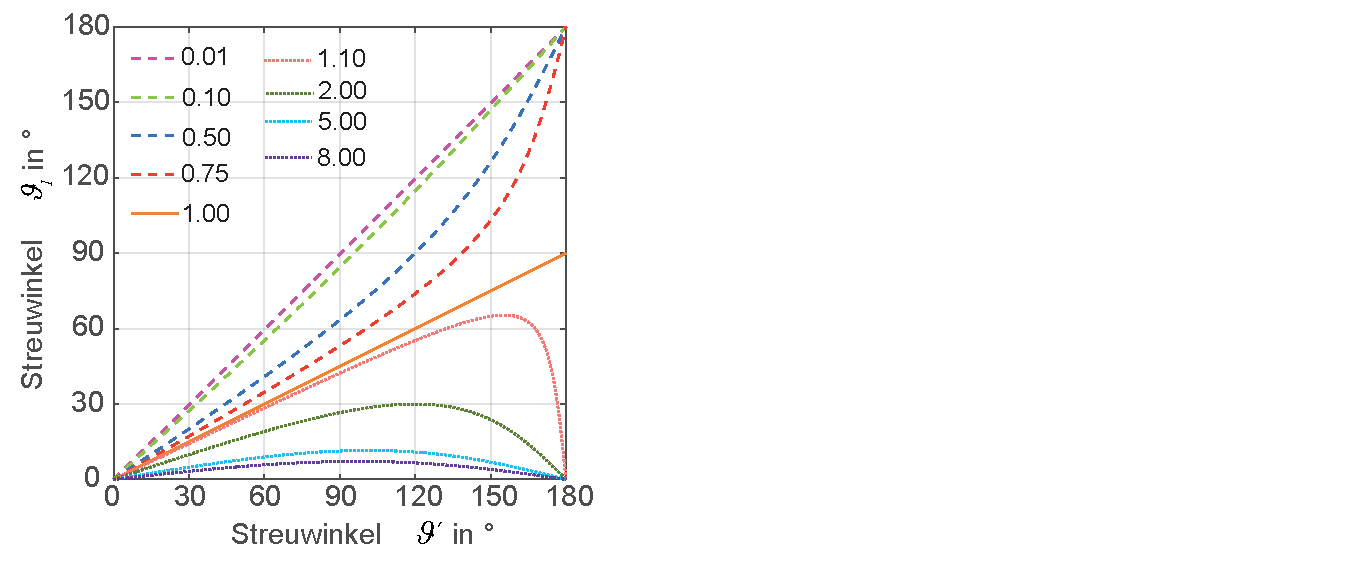
\includegraphics[width=\textwidth]{StreuwinkelUmrechnung.pdf}
\caption[Umrechnung von Streuwinkeln.]{Umrechnung des Streuwinkels $\vartheta'$ aus dem Schwerpunktsystem in den Streuwinkel $\vartheta_1$ im Laborsystem als Funktion verschiedener Massenverh�ltnisse $m_1/m_2$. Die Masse $m_2$ wird vor dem Sto� als ruhend angenommen. Vergleiche Gl. \eqref{eq:bew_Streuung7}.}
\label{abb:bew_StreuwinkelUmrechnung}
\end{figure}

\begin{figure}
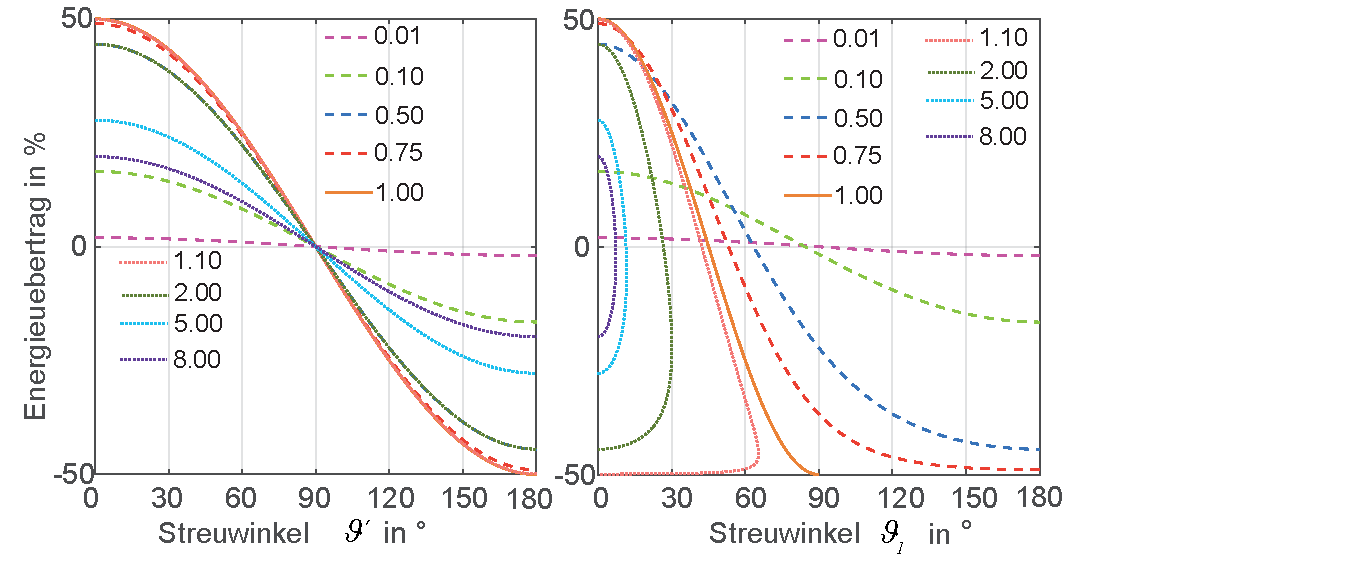
\includegraphics[width=\textwidth]{EnergieUebertrag.pdf}
\caption[Energie�bertrag beim elastischen Sto�.]{Energie�bertrag beim elastischen Sto� als Funktion verschiedener Massenverh�ltnisse $m_1/m_2$ als Funktion der Streuwinkels $\vartheta$ \bzw $\vartheta'$. Die Masse $m_2$ wird vor dem Sto� als ruhend angenommen. Vergleiche Gl. \eqref{eq:bew_Streuung9}.}
\label{abb:bew_EnergieUebertrag}
\end{figure}

\subparagraph{\textbf{Streuwinkel und Wirkungsquerschnitte bei Streuung im Zentralkraftfeld}}

Bisher haben wir f�r die \pot{}e nur angenommen, dass sie im Unendlichen verschwinden und haben daraus ein paar grunds�tzliche Eigenschaften der Streuung hergeleitet.
Wir wollen nun bestimmte Formen des Wechselwirkungs\potsuf{}s sowie der Energie und des (Dreh-)Impulses des einfallenden Teilchens annehmen.
Als Messgr��e bei der Streuung ermittelt man im Allgemeinen, wie viele Teilchen eines einfallenden Stromes von Teilchen durch ein Streuzentrum unter einem bestimmten Streuwinkel abgelenkt \bzw gestreut werden.
Wir nehmen wieder an, dass das Teilchen aus dem Unendlichen kommt und in das Wechselwirkungs\potsuf{} $U$ des Teilchens mit Masse $m_2$ gelangt.
Wir wollen ferner f�r das \pot{} ein Zentralkraft\potsuf{} annehmen, das also nur vom relativen Abstand der beiden Teilchen abh�ngt.
Wir k�nnen das System dann durch das �quivalente Einteilchenproblem (siehe \kap{bew_ZKP_EEKP}) mit der effektiven Masse $m_\text{eff}$ im Schwerpunktsystem $\vec{\Sigma}_\text{S}$ beschreiben.
Dann gilt f�r die Erhaltungsgr��e Energie 
\begin{align}
	E = \frac{m_\text{eff}}{2}\: v_\infty^2\,, \label{eq:bew_Streuung10}
\end{align}
mit $v_\infty$ als Relativgeschwindigkeit im Unendlichen.
F�r den ebenfalls konstanten Betrag des Drehimpulses gilt
\begin{align}
	L = b\:m_\text{eff}\:v_\infty \,, \label{eq:bew_Streuung11}
\end{align}
wobei $b' = b$ wieder der bereits eingef�hrte Sto�parameter\index{Sto�parameter} (\figref{bew_Streuwinkel}) ist, der in den beiden Systemen �bereinstimmt.
Wegen \eqref{eq:bew_Streuung8} ist $E > 0$ und die Teilchenbahn eine Hyperbel.
Der Streuwinkel $\vartheta'$ kann nach \eqref{eq:bew_Bahn_implizit1} mit $ r \rightarrow \infty $ berechnet werden zu
\begin{align}
	\vartheta' = \pi - \Delta \varphi = \pi - 2 b \int\limits_{r_\text{min}}^\infty \frac{\D r'}{r'^2 \sqrt{1-\frac{b^2}{r'^2}-\frac{U(r')}{E}}}\,. \label{eq:bew_Streuung12}
\end{align}
Hierbei haben wir die Ausdr�cke f�r die Energie \eqref{eq:bew_Streuung10} und den Drehimpuls \eqref{eq:bew_Streuung11} benutzt.
Wenn man also das Wechselwirkungs\potsuf{} $U(r)$ und die Energie $E$ eines einfallenden Streuteilchens kennt, h�ngt der Streuwinkel nur noch vom Sto�parameter $b$ ab.
Andererseits kann man R�ckschl�sse �ber das \pot{} erlangen, indem man $\vartheta$ als Funktion von $b$ misst.
Genau das war die Idee des ber�hmten Streuexperimentes von Rutherford.\footnote{Sir Ernest Rutherford\indexp{Rutherford, Sir Ernest} (1871--1937) war ein britisch-neuseel�ndischer Physiker. Als einer der bedeutendsten Experimentalphysiker erhielt er 1908 den Nobelpreis f�r Chemie (sic!) und sein wichtigster Beitrag zur Atomphysik ist das nach ihm benannte Atommodell, welches er 1911 aus seinen Streuversuchen von $\alpha$-Teilchen an Goldfolie herleitete.}
In diesem Experiment war das Wechselwirkungs\potsuf{} ein \gls{coulpot}
$U(r) = -\alpha/r$ und man erh�lt durch Einsetzen von
$\Delta \varphi_\infty = 2 \arccos(-1/\epsilon)$ und $\epsilon$ aus
\eqref{eq:bew_Bahn_Parameter} in \eqref{eq:bew_Streuung12}
sowie Ausdr�cken des Drehimpulses mithilfe des Sto�parameters $b$
verm�ge \eqref{eq:bew_Streuung11} die Abh�ngigkeit des Streuwinkels von der Energie und dem Streuparameter:
\begin{align}
	\sin^2\lk \frac{\vartheta'}{2} \rk & \:=\: \frac{1}{1 + \frac{4 E^2 b^2}{\alpha^2}}\,. \label{eq:bew_Streuung13}
\end{align}
Oft wird auch der Streuparameter als Funktion des Streuwinkels angegeben:
\begin{align}
	b^2 & \:=\: \lk \frac{1}{\sin^2\lk \frac{\vartheta'}{2} \rk } -1 \rk \frac{\alpha^2}{4 E^2}\,. \label{eq:bew_Streuung13a}
\end{align}
\begin{figure}
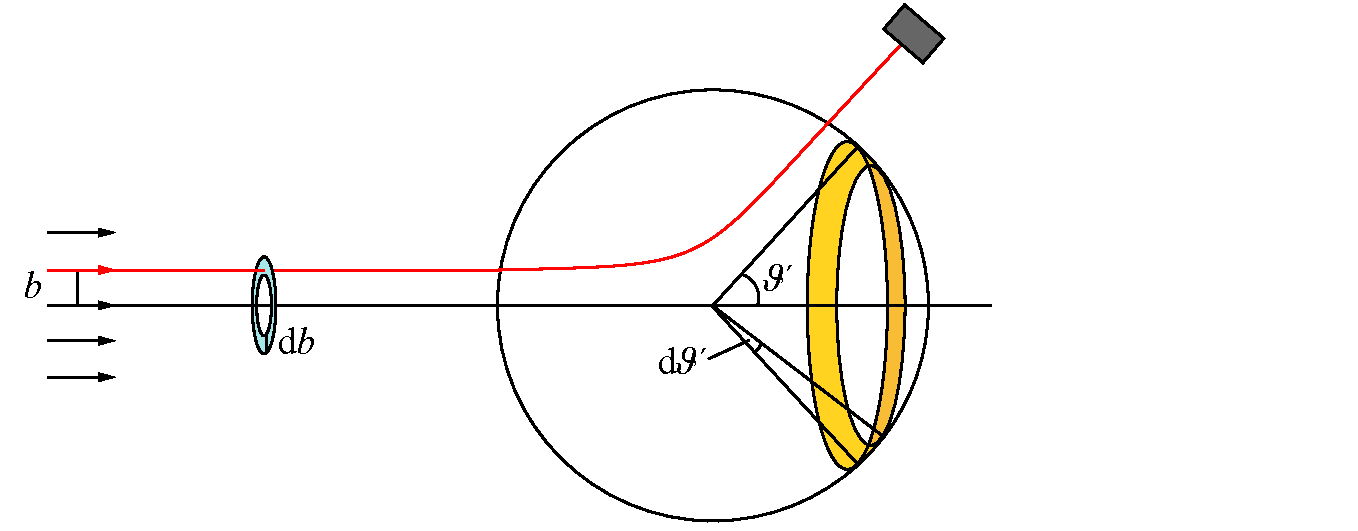
\includegraphics[width=\textwidth]{Wirkungsquerschnitt.pdf}
\caption[Geometrie der Streuung im Zentralkraftfeld und Wirkungsquerschnitt.]{Geometrie einer Streuung im Zentralkraftfeld und Wirkungsquerschnitt.}
\label{abb:bew_Wirkungsquerschnitt}
\end{figure}

Wir betrachten nun einen homogenen, konstanten Teilchenstrahl mit Teilchenstromdichte $I = N/(\Delta t \Delta A)$ in einem Zeitintervall $\Delta t$ und pro Fl�che $\Delta A$ (\figref{bew_Wirkungsquerschnitt}). 
Als Messgr��e im Streuexperiment wird die am Detektor pro Zeitintervall $\Delta t$ gemessene Anzahl von Streuteilchen $n(\vartheta')$ definiert.
Diese ist proportional zum Teilchenstrom $I$ und auch zur Detektorfl�che $\D\Omega$%
\footnote{Diese kann auch als Raumwinkelelement aufgefasst werden.}.
Der entsprechende Proportionalit�tsfaktor wird als differentieller Wirkungsquerschnitt\index{Wirkungsquerschnitt!differentieller} bezeichnet und folgenderma�en geschrieben:
\begin{align}
	\frac{\D \sigma'}{\D \Omega}  \:=\: \frac{n(\vartheta')}{I \Delta t \D \Omega}\,. \label{eq:bew_Streuung14}
\end{align}
Der totale Wirkungsquerschnitt\index{Wirkungsquerschnitt!totaler} ergibt sich dann als komplettes Raumwinkelintegral (bei Annahme einer Zylindersymmetrie) zu
\begin{align}
	\sigma' \:= \int \frac{\D \sigma'}{\D \Omega} \D \Omega = 2 \pi \int\nolimits_{0}^{\pi} \sin\vartheta' \D \vartheta' \frac{\D \sigma'}{\D \Omega}\,. \label{eq:bew_Streuung15}
\end{align}
Der totale Wirkungsquerschnitt ist quasi die \textit{effektive} Fl�che, an welcher der einfallende Teilchenstrom gestreut wird.
Man kann sowohl den differentiellen als auch den totalen Wirkungsquerschnitt in Beziehung zum Sto�parameter $b$ setzen.
Wir betrachten wieder \figref{bew_Wirkungsquerschnitt} und speziell den Kreisring mit der Fl�che $2 \pi b \D b$ des einfallenden Teilchenstromes (im Sto�parameterbereich $\left[b, b +\D b\right]$), der in den Raumwinkelbereich $\left[\vartheta', \vartheta' +\D \vartheta'\right]$ gestreut wird.
Wegen Teilchenerhaltung gilt\footnote{Man mache sich klar, dass die Absolutbetr�ge notwendig sind, da $\D b$ und $\D \vartheta'$ unterschiedliche Vor\-zei\-chen haben k�nnen.}
	\[I \lk 2 \pi b \left|\D b\right| \rk = I \lk 2 \pi \sin \vartheta' \frac{\D \sigma}{\D \Omega} \left| \D \vartheta' \right| \rk\,.
\]
Der differentielle Wirkungsquerschnitt h�ngt demnach mit dem Sto�parameter und dem Streuwinkel $\vartheta'$ wie folgt zusammen, wobei $b(\vartheta')$ f�r ein bestimmtes \pot{} aus \eqref{eq:bew_Streuung12} berechnet werden kann:
\begin{align}
	\frac{\D \sigma'}{\D \Omega}  =  \frac{b(\vartheta')}{\sin\vartheta'} \left| \frac{\D b(\vartheta')}{\D\vartheta'} \right| = \frac{1}{2 \sin\vartheta'} \left| \frac{\D b^2(\vartheta')}{\D\vartheta'} \right|\,. \label{eq:bew_Streuung16}
\end{align}
Die Messungen von Streuexperimenten liegen aber als Gr��en des Laborsystems $\vec{\Sigma}_\text{L}$ vor,
in denen das Streuzentrum ($m_2$) und der Detektor zumeist fest sind.
Daher
unterscheiden sich die differentiellen Streuquerschnitte in beiden Systemen und m�ssen mit der Beziehung \eqref{eq:bew_Streuung7} f�r die Streuwinkel umgerechnet werden.
Man erh�lt dann 
\begin{align}
	\frac{\D \sigma}{\D \Omega} = \frac{\D \sigma'}{\D \Omega} \left| \frac{\D \cos\vartheta'}{\D \cos\vartheta} \right| \,, \label{eq:bew_Streuung17}
\end{align}
worin die ungestrichenen Gr��en wie gehabt die Gr��en im Laborsystem darstellen.
Wir wollen zum Abschluss im folgenden Beispiel noch die Wirkungsquerschnitte f�r das Coulomb-Potential  berechnen, die der Form nach nat�rlich auch denen des Newtonschen Gravitations\potsuf{}s entsprechen.

%BEISPIEL 1 %%%%%%%%%%%%%%%%%%%%%%%%%%%%%%%%%%%%%%%%%%%%%%%%%%%%%%%%%%%%%%%%%%%%%%%%%%%%%%%%%%
\begin{example}{Wirkungsquerschnitte f�r Streuung in Zentralkraftfeldern (Coulomb-Potential)}
Mit $U(r) = -\alpha/r$ kann man zun�chst $b^2(\vartheta')$ nach \eqref{eq:bew_Streuung13} berechnen und davon die Ableitung bilden:
	\[ \left| \frac{\D b^2(\vartheta')}{\D\vartheta'} \right| = \frac{\alpha^2}{4 E^2} \frac{\cos\frac{\vartheta'}{2}}{\sin^3\frac{\vartheta'}{2}} = \frac{\alpha^2}{8 E^2} \frac{\sin\vartheta'}{\sin^4\frac{\vartheta'}{2}}\,.
\] 
Hierin ist $E$ die Energie des Teilchens.
Daraus folgt der differentielle Rutherford-Wirkungsquerschnitt\index{Wirkungsquerschnitt!Rutherford-} im Schwerpunktsystem
\begin{align}
	\frac{\D \sigma'}{\D \Omega}  = \lk \frac{\alpha}{4 E} \rk^2 \frac{1}{\sin^4\lk\vartheta'/2\rk} \,. 	\label{eq:bew_Streuung18}
\end{align}
Dies ist die  ber�hmte Streuformel von Rutherford\index{Streuformel!Rutherford-}. Der totale Wirkungsquerschnitt f�r das $U(r) = \alpha/r$-\pot{} ergibt sich durch Integration �ber $\vartheta'$ zu
\begin{align}
	\sigma' = 2 \pi \lk \frac{\alpha}{4 E} \rk^2 \int\limits_0^\pi \frac{\D \vartheta' \,\sin\vartheta'}{\sin^4\lk\vartheta'/2\rk} = \infty \,. 	\label{eq:bew_Streuung19}
\end{align}
und ist unendlich gro�, was schnell klar wird, da das \pot{} auch in beliebig gro�er Entfernung noch Teilchen streut.
Dies erkennt man auch daran, dass der differentielle Wirkungsquerschnitt f�r $\vartheta'=0$ divergiert.
In der Realit�t gibt es nat�rlich keine punktf�rmigen Streuzentren.
Entweder haben die Zentren eine Ausdehnung oder sie werden wie beim Atom teilweise abgeschirmt.
\label{bsp:SigmaCoulomb}
\end{example}
%BEISPIEL %%%%%%%%%%%%%%%%%%%%%%%%%%%%%%%%%%%%%%%%%%%%%%%%%%%%%%%%%%%%%%%%%%%%%%%%%%%%%%%%%%


\subsubsection{$N$-K�rper-Systeme}\index{Mehrk�rperproblem} \index{Streuung} \label{kap:bew_n_body}

Im Kapitel Himmelsmechanik (Band II, Kapitel 3) werden wir
viele F�lle kennenlernen, die nicht mehr als Zweik�rperproblem
modelliert werden k�nnen.
Das Mehrk�rper- oder $N$-K�rperproblem ist f�r $N>2$ nicht in analytischer Form l�sbar, man kann es aber mit st�rungstheoretischen Ans�tzen angehen.
Dabei betrachtet man das Problem zun�chst als Zweik�rpersystem und bezieht dann die Einfl�sse der weiteren K�rper \bzw Massen als St�rungen mit ein.
Ist das Zweik�rperproblem beispielsweise das Sonne-Erde-System, so lassen sich die Einfl�sse der anderen Planeten auf die Erdbahn auf diese Weise absch�tzen.
Allerdings ist dieser Ansatz nur dann erfolgversprechend,
wenn die St�rungen gering sind.
In anderen F�llen muss man auf numerische Verfahren zur�ckgreifen (siehe \zb \cite{Dehnen2011}).
Wir werden in der Himmelsmechanik sowohl st�rungstheoretische als auch numerische Methoden f�r die Berechnung der Planetenbewegung anwenden. 
Zus�tzlich wollen wir uns hier kurz mit einem Spezialfall
des Dreik�rperproblems besch�ftigen,
welcher trotz seiner begrenzenden Annahmen von gro�er Bedeutung f�r
das Verst�ndnis der Mechanik des Sonnensystems und �hnlicher Probleme ist.

\subsubsection{Das eingeschr�nkte Drei-K�rper-System}\index{Dreik�rperproblem} \index{Dreik�rperproblem!reduziertes} \index{Dreik�rperproblem!eingeschr�nktes}\label{kap:bew_3_body}

\begin{figure}%
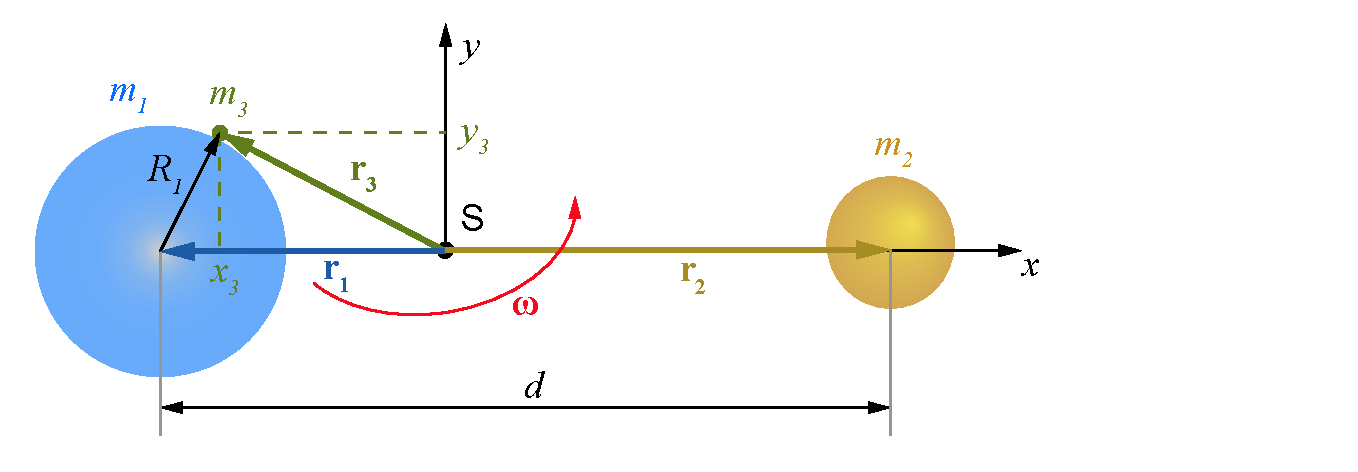
\includegraphics[width=\textwidth]{Geometrie3KP.pdf}%
\caption[Geometrie des reduzierten Dreik�rperproblems.]{Geometrie des reduzierten Dreik�rperproblems.}%
\label{abb:bew_3KoerperP01}%
\end{figure}

Wir betrachten in \figref{bew_3KoerperP01} die Geometrie des sogenannten eingeschr�nkten  Dreik�rperproblems.
Es soll gelten $m_3 \ll m_1,m_2$.
Die Masse $m_1$ k�nnte \zb die Sonnenmasse $m_{\astrosun}$ und die Masse $m_2$ gleich der Erdmasse $m_{\earth}$ sein.
Die kleine Masse $m_3$ w�re dann \zb ein Satellit oder ein Asteroid.
Wir definieren zur Vereinfachung
		\begin{align}
				p = \frac{m_1}{m_1+m_2}<1 \qquad \text{und} \qquad 1-p= \frac{m_2}{m_1+m_2}<1 \,. \label{eq:bew_red3KP01}
		\end{align}
Damit haben im mitrotierenden Schwerpunktsystem $\vec{\Sigma}'$ die Massen $m_1$ und $m_2$ die Koordinaten\footnote{Der Einfachheit halber lassen wir in \kap{bew_3_body} 
%und Kap. \label{kap:gezeiten}
 die Striche an den Koordinatengr��en im mitbewegten \KOS{} weg, da wir ausschlie�lich in diesen System bleiben.}:
		\begin{align}
				\vec{r}_1 = 
				\begin{pmatrix}
				(p-1)d  \\
				0 \\
				0 
				\end{pmatrix}
~~~~				\text{und} \quad
				r_2 = 
				\begin{pmatrix}
				p\,d  \\
				0 \\
				0 
				\end{pmatrix}
				\,.
				\label{eq:bew_red3KP02}
		\end{align}
Die Umlaufzeit \bzw Rotationsfrequenz von $m_1$ und $m_2$ ergibt sich zu
		\begin{align}
				T^2 = \frac{4 \pi^2 d^3}{G(m_1+m_2)} \quad \text{\bzw}\quad \vec{\omega}=\frac{2 \pi}{T} = 
				\begin{pmatrix}
				0  \\
				0 \\
				\sqrt{\frac{G(m_1+m_2)}{d^3}}
				\end{pmatrix}
				\,.
				\label{eq:bew_red3KP03}
		\end{align}
Aus \figref{bew_3KoerperP01} lesen wir ferner ab:
        \begin{align}
		\begin{split}
				\left| \vec{r}_1 - \vec{r}_3 \right| = d_1 &= \sqrt{(x_3-(p-1)d)^2+{y_3}^2} \,,  \\
				\left| \vec{r}_2 - \vec{r}_3 \right| = d_2 &= \sqrt{(x_3-p\,d)^2+{y_3}^2}  \,.
		\end{split}
		\label{eq:bew_red3KP04}
        \end{align}
Da wir uns in einem mit $\vec{\omega} = \omega\kern1pt\vec{e}_3$ mitrotierenden Koordinatensystem befinden, m�ssen wir die Scheinkr�fte Zentrifugalkraft und Coriolis-Kraft ber�cksichtigen.\\
F�r $\ddot{\vec{r}}_3$ gilt dann
\begin{align}
                \ddot{\vec{r}}_3 &= -2\:\vec{\omega}\times\dot{\vec{r}}_3-\vec{\omega}\times(\vec{\omega}\times\vec{r}_3)-\frac{\gradv U(\vec{r}_3)}{m_3}\,, \label{eq:bew_red3KP05}
\end{align}
wobei 
	\[U(\vec{r}_3) = -\frac{G\,m_1 m_3}{d_1}-\frac{G\,m_2 m_3}{d_2} 
	\]
ist.
F�hrt man die Vektormultiplikationen  in \eqref{eq:bew_red3KP05} aus, so erh�lt man mit dem wie folgt definierten effektiven \pot{} 
		\begin{align}
		\begin{split}
				\frac{U_\text{eff}}{m_3} &= \frac{U(\vec{r}_3)}{m_3}-\frac{\omega^2}{2}({x_3}^2+{y_3}^2) \\
				&= -\frac{G\,m_1}{d_1(x_3,y_3)}-\frac{G\,m_2}{d_2(x_3,y_3)}-\frac{G\,(m_1+m_2)}{2d^3}\,({x_3}^2+{y_3}^2)\,,
		\end{split}	
		\label{eq:bew_red3KP06}
		\end{align}
die Bewegungsgleichungen
\begin{align}
		\begin{split}
				\ddot{x}_3-2\omega\dot{y}_3 &= -\frac{1}{m_3}\frac{\d U_\text{eff}}{\d x_3} \,, \\
				\ddot{y}_3+2\omega\dot{x}_3 &= -\frac{1}{m_3}\frac{\d U_\text{eff}}{\d y_3} \,.
		\end{split}	
		\label{eq:bew_red3KP07}
		\end{align}
Diese kann man mit den bekannten numerischen Methoden l�sen.
Wir wollen aber zun�chst die Bereiche $(x_3,y_3)$ bestimmen, in denen �berhaupt eine L�sung existieren kann, oder m.a.W. in denen sich die Masse $m_3$ befinden kann. \\
Multipliziert man die erste Gleichung von \eqref{eq:bew_red3KP07} mit $\dot{x}_3$ und die zweite mit $\dot{y}_3$ und addiert beide, erhalten wir die folgende Differentialgleichung:
\begin{align}
	 \frac{\D}{\D t}\underbrace{\lk\frac{1}{2}({\dot{x}_3}{}^2+{\dot{y}_3}{}^2)+\frac{1}{m_3} U_\text{eff}\rk}_{-\frac{1}{2}\mathcal{C}}= 0\,.
\end{align}
%Dazu bilden wir:
%\begin{center}
%\begin{tabular}{C{4.5cm}|C{0.5cm}} 
 %$\ddot{x}_3\dot{x}_3-2\omega\dot{y}_3\dot{x}_3 = -\frac{1}{m_3} \frac{\d U_\text{eff}}{\d x_3}\dot{x}_3$ &  \\ 
 %\rule{0pt}{15pt}$\ddot{y}_3\dot{y}_3+2\omega\dot{x}_3\dot{y}_3 = -\frac{1}{m_3} \frac{\d U_\text{eff}}{\d y_3}\dot{y}_3$ & $+$ \\ 
 %\rule{0pt}{0pt} & \\
 %\hline
 %\rule{0pt}{0pt} & \\
 %$\frac{\D}{\D t}\underbrace{\lk\frac{1}{2}({\dot{x}_3}^2+{\dot{y}_3}^2)+\frac{1}{m_3} U_\text{eff}\rk}_{-\frac{1}{2}\mathcal{C}}= 0$ &  
%\label{eq:bew_red3KP08}
%\end{tabular}
%\end{center}
Die Gr��e 
		\begin{align}
				\mathcal{C} = -\lk {\dot{x}_3}{}^2+{\dot{y}_3}{}^2 \rk - \frac{2U_\text{eff}}{m_3} = \omega^2 \lk {x_3}^2+{y_3}^2 \rk-\frac{2U}{m_3}-\lk{{\dot{x}_3}{}}^2+{\dot{y}_3{}}^2\rk \label{eq:bew_red3KP09}
		\end{align}
ist also eine Erhaltungsgr��e und wird \emph{Jacobi}\footnote{Carl Gustav Jacob Jacobi (1804--1851) war einer deutscher Mathematiker, der zu den produktivsten und vielseitigsten Mathematikern z�hlt. Besonders seine Theorie der elliptischen Funktionen, aber auch seine Arbeiten zur Differentialgeometrie waren f�r die mathematischen Physik wegbereitend.
Die Hamilton-Jacobi-Theorie der klassischen Mechanik war eine wichtige Vorstufe f�r den sp�teren �bergang zur Quantenmechanik.}\indexp{Jacobi, Carl Gustav Jacob}\index{Jacobi-Konstante}\emph{-Konstante} genannt. Diese Konstante ist die einzige Erhaltungsgr��e f�r das reduzierte Dreik�rperproblem und definiert den m�glichen Bereich der Bewegung der Masse $m_3$ eindeutig. \\
Offensichtlich gilt in \eqref{eq:bew_red3KP09} immer ${\dot{x}_3{}}^2+{\dot{y}_3{}}^2 \geq 0$.
Damit muss $\mathcal{C}+2U_\text{eff}/m_3 \leq 0$ sein, was die sogenannte \textit{Hill-Kurve} \index{Hill-Kurve} als die Menge aller Punkte $ \lk x_3,y_3 \rk $ festlegt, f�r die $U_\text{eff}\,(x_3,y_3) \leq - m_3\,C/2$ ist.
\figref{bew_3KoerperP02} zeigt diesen Bereich (siehe auch \probref{bew_HillLagrangePkt} und \mscr{} \mlbewref{LagrangePunkte.m}).
Besonders interessant sind in diesem Bereich die Punkte $\lk x_3^{(\text{L})},y_3^{(\text{L})}\rk $, an denen die Masse $m_3$ relativ zu den Massen $m_1$ und $m_2$ (im mitbewegten Koordinatensystem) in Ruhe ist.
Diese Punkte werden \textit{Lagrange-Punkte}%
\footnote{Diese Lagrange-Punkte spielen in der Raumfahrt
eine gro�e Rolle.}\index{Lagrange-Punkte}
genannt und sind definiert durch $\gradv U_\text{eff}= 0$,
da dann aus den Bewegungsgleichungen \eqref{eq:bew_red3KP07}
f�r $\dot{x}_3= \dot{y}_3= 0$ folgt:
    \begin{align}
        \begin{split}
            0 &= \omega^2x_3^{(\text{L})}-\frac{G\,m_1(x_3^{(\text{L})}-x_1)}{{d_1}^3} -\frac{G\,m_2(x_3^{(\text{L})}-x_2)}{{d_2}^3} \,, \\
            0 &= \omega^2 y_3^{(\text{L})}-\frac{G\,m_1 y_3^{(\text{L})}}{{d_1}^3}-\frac{G\,m_2y_3^{(\text{L})}}{{d_2}^3} \,.
        \end{split}
        \label{eq:bew_red3KP10}
    \end{align}
Aus diesen beiden Gleichungen bestimmt man dann die Werte $\lk x_3^{(\text{L})},y_3^{(\text{L})} \rk$, zun�chst f�r $y_3^{(\text{L})}= 0$.\footnote{Man beachte, dass die Gr��en $d_1, d_2$ von $x_3, y_3$ abh�ngen.} Man erh�lt die Lagrange-Punkte $L_1, L_2$ und $L_3$. \\
F�r die Berechnung eines weiteren Paares von Lagrange-Punkten $L_4, L_5$ f�r $y_3^{(\text{L})}\neq 0$ multipliziert man die zweite Gleichung in \eqref{eq:bew_red3KP10} mit $x_3^{(\text{L})}/y_3^{(\text{L})}$, subtrahiert diese von der ersten Gleichung und erh�lt zun�chst
		\begin{align*}
				\frac{G\,m_1x_1}{{d_1}^3}+\frac{G\,m_2y_1}{{d_2}^3} = 0 \,,
		\end{align*}
und daraus
		\begin{align*}
				d_1^{(\text{L})} = d_2^{(\text{L})} = d \,.
		\end{align*}

\begin{figure}%
\includegraphics[width=\textwidth]{LagrangePt.pdf}%
\caption[Hill-Kurve und Lagrange-Punkte des reduzierten Dreik�rperproblems.]{Hill-Kurve und Lagrange-Punkte des reduzierten Dreik�rperproblems. \fa Massenverh�ltnis 40:1, \fb Massenverh�ltnis Sonne-Jupiter.}%
\label{abb:bew_3KoerperP02}%
\end{figure}

Die Lagrange-Punkte $L_4, L_5$ bilden also mit den Massen $m_1$ und $m_2$ jeweils gleichseitige Dreiecke. In \probref{bew_HillLagrangePkt} berechnen wir die Lagrange-Punkte $L_1$ bis $L_5$ und untersuchen deren Stabilit�t. Das Ergebnis der Berechnung ist in \figref{bew_3KoerperP02} eingezeichnet.

\subsubsection{Gezeiten} \label{kap:bew_gezeiten}

Gezeitenkr�fte sind im Sprachgebrauch h�ufig mit dem Ph�nomen von Ebbe und Flut auf den Ozeanen der Erde verkn�pft.
Sie sind aber viel fundamentaler und treten �berall dort auf, wo die r�umliche Ausdehnung der K�rper in einem gravitativen System nicht mehr zu vernachl�ssigen ist oder anders gesprochen die Inhomogenit�t des Gravitationsfeldes zum Tragen kommt.
Im Umkehrschluss treten Gezeitenkr�fte bei idealisierten Systemen von Punktmassen nicht auf.
Wir wollen hier im Abschnitt �ber Massepunkte einen �berblick �ber das Thema und eine grunds�tzliche Einf�hrung geben.
In der Himmelsmechanik werden wir uns dann
genauer mit einigen Ph�nomenen der Gezeiten besch�ftigen, insbesondere
mit dem Erde-Mond-System, den Gezeiten der Ozeane und auch der dabei auftretenden
Gezeitenreibung. Hier wollen wir nur das Grundprinzip der Gezeiten erl�utern.\\
Wir betrachten die Geometrie zum Gezeitenproblem in \figref{bew_3KoerperPGezeiten}. In unserer Betrachtung eines Zweik�rperproblems mit Gezeiten wollen wir dabei einen K�rper als kugelf�rmig ansehen (Masse $m_1$, Radius $R$) und den anderen als punktf�rmig (Masse $m_2$).
Wenn wir die Dynamik des ausgedehnten K�rpers durch eine im Schwerpunkt konzentrierte Masse $m_1$ beschreiben, k�nnen wir weiterhin die Bewegungsgleichungen des ZKP verwenden.%
\footnote{Allerdings gilt dies nur dann, wenn die Gezeitenkr�fte im Vergleich zu den inneren Kr�ften des ausgedehnten K�rpers vernachl�ssigt werden k�nnen. Das ist vielfach nicht der Fall, aber bei der Betrachtung der Gezeitenwirkung auf die Ozeane in Form von Ebbe und Flut gegeben.}  Die Punktmasse $m_2$ hat das \pot{}
		\begin{align}
				U\!\lk\vec{r}\rk = - \frac{G\,m_2}{|\vec{r}-\vec{r}_2|} \,. \label{eq:bew_Gezeiten01}
		\end{align}
Damit wirkt auf eine kleine Testmasse $m$ am Ort $\vec{r}$ die Kraft
		\begin{align*}
				\vec{F}\!\lk\vec{r}\rk = -m\,\gradv\,U\lk\vec{r}\rk \,.
		\end{align*}
Damit ist klar, dass zwei gleiche Testmassen $m$, die sich an unterschiedlichen Positionen auf dem ausgedehnten K�rper $m_1$ befinden, unterschiedlich gro�en Kr�ften von der Masse $m_2$ unterliegen. \\
Wir wollen zur Berechnung dieser Kr�fte dazu die Kraft $\vec{F}\!\lk\vec{r}\rk$ um den Schwerpunkt der Masse $m_1$ entwickeln und schreiben
		\begin{align}
				\vec{F}\!\lk\vec{r}\rk = \vec{F}\!\lk\vec{r}_1+\delta\,\vec{r}\rk =\vec{F}\!\lk\vec{r}_1\rk+\lk\delta\vec{r}\,\cdot\,\gradv\rk \vec{F}\!\lk\vec{r_1}\rk+ \cdots \,. \label{eq:bew_Gezeiten02}
		\end{align}

\begin{figure}%
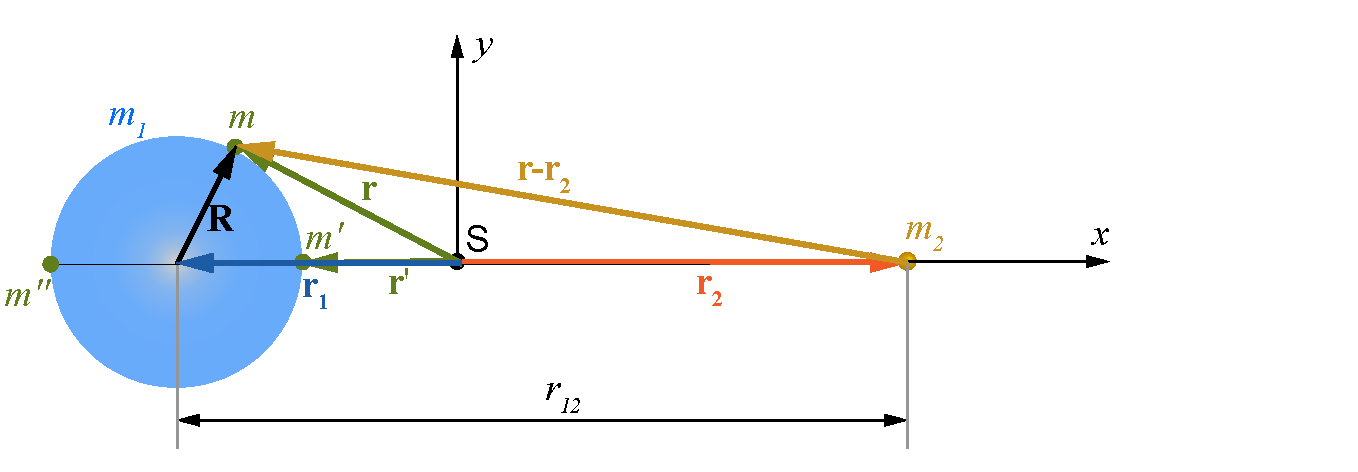
\includegraphics[width=\textwidth]{GeometrieGezeiten.pdf}%
\caption[Geometrie des Gezeitenproblems.]{Geometrie des Gezeitenproblems.}%
\label{abb:bew_3KoerperPGezeiten}%
\end{figure}

F�r das Erde-Mond-System kann man in guter N�herung $r_1=0,\,r_2=r_{12}=r_\text{EM}$ annehmen, f�r das Erde-Sonne-System in sehr guter N�herung $r_2 =0,\,r_1=r_{12}= r_\text{ES}$. Da die weiteren Betrachtungen auch \zb f�r Doppelsternsysteme anwendbar sein sollen, bei denen $m_1 \approx m_2$ gelten kann, schreiben wir allgemeiner

	\begin{align*}
			\vec{F}\!\lk\vec{r}\rk = -m\,\gradv\, U\lk\vec{r}\rk = -m\lk \frac{\d}{\d x}U\lk\vec{r}\rk, \frac{\d}{\d y}U\lk\vec{r}\rk, \frac{\d}{\d z}U\lk\vec{r}\rk\rk \,,
	\end{align*}
den Vektor $\vec{r}_1 = x\,\vec{e}_x+y\,\vec{e}_y+z\,\vec{e}_z$ , sowie das Skalarprodukt von $\delta\vec{r}$ und $\gradv$ als
	\begin{align*}
			\delta\vec{r}\cdot \gradv &= \D x\,\frac{\d}{\d x}+ \D y\,\frac{\d}{\d y}+\D z\,\frac{\d}{\d z} = \sum\limits_{i}^3 \D x_i\,\frac{\d}{\d x_i} = \D x_i\,\frac{\d}{\d x_i}\,.
	\end{align*}
Dann kann man die Gezeitenkraft \eqref{eq:bew_Gezeiten02} schreiben als
        \begin{align}
				\Delta \vec{F}_\text{Gez} &= \vec{F}\!\lk\vec{r}_1+\delta\,\vec{r}\rk-\vec{F}\!\lk\vec{r}_1\rk = \delta \vec{r}\cdot\gradv\vec{F}(\vec{r}_1) = -m \sum\limits_{i}^3 \sum\limits_{j}^3 \D x_j \, \frac{\d^2 U(\vec{r})}{\d x_i\,\d x_j }\,\vec{e}_i \nonumber \\
				&= -m\, \sum\limits_{i}^3 \sum\limits_{j}^3 \D x_j\,H_{ij} \,\vec{e}_i = -m\, \D x_j\,H_{ij} \,\vec{e}_i \,, \label{eq:bew_Gezeiten03}
\end{align}
wobei wir im letzten Schritt mit $\mathbb{H} \equiv H_{ij}$  ist die sogenannte Hesse-Matrix\footnote{Otto Hesse\indexp{Hesse, Otto} (1811--1874) war ein deutscher Mathematiker, der vor allem auf dem Gebiet der analytischen Geometrie arbeitete.} eingef�hrt und die Einsteinsche Summenkonvention benutzt haben. \\
Die vollst�ndige Hesse-Matrix in kartesischen Koordinaten ausgeschrieben lautet 
\begin{align}
	H_{ij} = \frac{\d^2 U}{\d x_i \d x_j} = 
\begin{pmatrix}
\frac{\d^2\, U}{\d\,x^2} & \frac{\d^2\, U}{\d x\,\d y}  & \frac{\d^2\, U}{\d x\,\d z} \\
\frac{\d^2\, U}{\d y\,\d x} & \frac{\d^2\, U}{\d\,y^2} & \frac{\d^2\, U}{\d y\,\d z} \\
\frac{\d^2\, U}{\d z\,\d x} & \frac{\d^2\, U}{\d z\,\d y} & \frac{\d^2\, U}{\d\,z^2}
\end{pmatrix} \,.
\label{eq:bew_Gezeiten04}
\end{align}
Gleichung \eqref{eq:bew_Gezeiten03} gilt ganz allgemein
f�r ein beliebiges \pot{}, \zb auch f�r eines mit mehreren Gravitationszentren,
und ist auch gut f�r die numerische Auswertung geeignet.
Man beachte aber, dass \eqref{eq:bew_Gezeiten03} eine Taylorentwicklung ist, weswegen f�r alle $i,j$ jeweils $\D x_j \ll \left| x_j - x_i \right| ~$ gelten muss. 
Wir wollen im Folgenden den einfachen Fall annehmen, dass die Testmasse auf der Verbindungsachse der beiden Massen $m_1$ und $m_2$ liegt.
Gleichung \eqref{eq:bew_Gezeiten03} sieht dann f�r die Masse $m'$ mit $\vec{r}' = \vec{r}_2-\vec{r}_1$ und $\delta\,\vec{r}\| \vec{r}'$ (wir betrachten ja nur die axiale Richtung) folgenderma�en aus:
		\begin{align}
				\Delta F_\text{Gez} = \Delta \vec{F}_\text{Gez}\cdot\vec{e}_z = \lk \frac{G\,m\,m_2}{\lk r_{12} \pm R_1\rk^2}\frac{\vec{r}}{|\vec{r}|} - \frac{G\,m\,m_2}{r_{12}{}^2}\frac{\vec{r}}{|\vec{r}|} \rk\cdot \vec{e}_z \,. \label{eq:bew_Gezeiten05}
		\end{align}
Da f�r den Radius des K�rpers mit der Masse $m_1$ aber $R \ll r_{12}$ gilt, k�nnen wir \eqref{eq:bew_Gezeiten05} entwickeln und erhalten
        \begin{align}
                \frac{1}{\lk r_{12} \pm R\rk^2}&\approx \frac{1}{r_{12}{}^2}\lk 1 \mp \frac{2R}{d}\rk \text{\quad und} \nonumber \\
                \Delta F_\text{Gez} &\approx \mp\frac{2G\,m\,m_2\,R}{r_{12}{}^3}\,.\label{eq:bew_Gezeiten06}
        \end{align}
Das Zeichen $+$ ist dabei f�r einen Probek�rper $m'$ zu verwenden,
der auf der Seite des ausgedehnten K�rpers liegt,
welche dem Ort der Masse $m_2$ zugewandt ist,
das Zeichen $-$ entsprechend f�r einen Probek�rper $m''$ auf der diesem Ort abgewandten Seite des K�rpers $m_1$.
Interessant ist der starke Abfall der Gezeitenkraft mit der dritten Potenz
des Abstandes zwischen den Massen $m_1$ und $m_2$.
Mit \eqref{eq:bew_Gezeiten06} kann man sofort das Verh�ltnis der Gezeitenkr�fte von Sonne und Mond auf einen K�rper auf der Erdoberfl�che berechnen:
		\begin{align*}
				\frac{\Delta {F_\text{Gez}}_\text{M}}{\Delta{F_\text{Gez}}_\text{S}} = \frac{m_\text{M}}{{a_{\text{EM}}}^3}\frac{{a_\text{ES}}^3}{m_\text{\text{S}}} \approx 2.18 \,.
		\end{align*}
Hier haben wir die Werte f�r die Mondmasse $m_\text{M} = \SI{7.346e22}{\kilogram}$, die Sonnenmasse $m_\text{S} = \SI{1.989e30}{\kilogram}$, den mittleren Abstand von Erde und Mond $a_\text{EM}= \SI{384.4e06}{\metre}$ und die sogenannte astronomische Einheit\index{Astronomische Einheit}\index{Astronomische Einheit} $a_\text{\earth} = a_\text{\text{ES}} = \SI{149.6e09}{\metre}$ benutzt.
Die Gezeitenwirkung des Mondes auf die Erde ist also etwa doppelt so gro� wie die der Sonne auf die Erde.
In \probref{bew_gezeiten01} wollen wir die Verformung eines Rings unter dem Einfluss von Gezeitenkr�ften berechnen. Den Ring beschreiben wir als Anordnung von 36 Testmassen, die im Schwerefeld einer gro�en Masse frei fallen.\\

\subsection{Lagrange-Formalismus}\index{Lagrange-Gleichung} \label{kap:bew_lagrange_formalism}

Bisher haben wir die Mechanik auf Basis der Newtonschen Axiome und der daraus folgenden Bewegungsgleichungen behandelt. Wir wollen jetzt den \emph{Lagrange-Formalismus}\index{Lagrange-Formalismus|textbf} kennen lernen, der 1788 von Lagrange\indexp{Lagrange, Joseph-Louis} eingef�hrt wurde und bei dem ein mechanisches System durch eine einzige skalare Funktion, die Lagrange-Funktion, beschrieben wird. Der Formalismus ist v�llig �quivalent zur Newtonschen Mechanik und ist dar�ber hinaus auch direkt auf beliebige Koordinatensysteme und beschleunigte Bezugssysteme anwendbar, ohne dass man eine zus�tzliche Betrachtung der Scheinkr�fte machen muss. Der Lagrange-Formalismus erlaubt damit die Wahl geeigneter generalisierter Koordinaten und vereinfacht dadurch die Behandlung vieler physikalische Probleme. Ebenso lassen sich im Gegensatz zur Newtonschen Mechanik Zwangsbedingungen relativ einfach ber�cksichtigen.

\subsubsection{Zwangsbedingungen}\index{Zwangsbedingungen} \label{kap:bew_zwangsbedingungen}

Die bisher gezeigten Anwendungen der Newtonschen Bewegungsgleichungen behandelten F�lle, in denen sich ein K�rper/Massepunkt frei, \dh nur unter dem Einfluss externer Kr�fte bewegen konnte.
H�ufig liegt aber Einschr�nkungen der Bewegungsfreiheit vor.
Eine solche nennt man dann eine \emph{\gls{zwangsbed}}.\footnote{Das kennen wir als Menschen ja auch sehr gut.} Zwangsbedingungen k�nnen f�r ein $N$-Teilchen-System in der Form
\begin{align}
	f_r(t, \vec{r_1},\vec{r_2},\ldots,\vec{r_N}) = 0 ~~, r = 1\ldots Z_B\,,\text{ wobei }Z_B \leq 3N  \label{eq:bew_holonome_ZB}
\end{align}
geschrieben werden, wodurch dann $ F = 3N -Z_B $ \emph{Freiheitsgrade}\index{Freiheitsgrad} der Bewegung verbleiben.
Als Beispiel sei die Bewegung auf einer schiefen Ebene genannt.
Da sich der Massepunkt entlang der Geraden $z = x \tan{\alpha}$ bewegen muss, lautet die Zwangsbedingung 
	\[f_1(0,x,y,z) = z - x \tan{\alpha} = 0
\]
und das System hat zwei verbleibende Freiheitsgrade $(x, y)$. Man kann nun unterscheiden in
\begin{itemize}
	\item \emph{holonom-skleronome} Zwangsbedingungen\index{Zwangsbedingung!holonom-skleronome}, die nicht explizit von der Zeit abh�ngen, also $\partial f_r/\partial t = 0$,
	\item \emph{holonom-rheonome} Zwangsbedingungen\index{Zwangsbedingung!holonom-rheonome}, die explizit von der Zeit abh�ngen, also $\partial f_r/\partial t \neq 0$,
	\item \emph{nicht-holonome} Zwangsbedingungen\index{Zwangsbedingung!nicht-holonome}, die sich nicht in der Form \eqref{eq:bew_holonome_ZB} schreiben lassen und daher die Anzahl der freien Koordinaten nicht reduzieren, wie 
	\begin{itemize}
		\item Zwangsbedingungen, die in der Form von Ungleichungen vorliegen, also 
			\[\tilde{f}(t, \vec{c}_1\cdot \D\vec{r_1},\vec{r_2},\ldots,\vec{r_N}) \leq 0
		\] 
		\item oder Zwangsbedingungen, die in nicht-integrierbarer differentieller Form 
			\[\delta \tilde{f} = \vec{c}_{k1}\cdot \D\vec{r_1} + \vec{c}_{k2}\cdot \D\vec{r_2} + \cdots + \vec{c}_{kN}\cdot  \D\vec{r_N} + \vec{c}_{kt} \D t = 0 \quad \text{mit}\quad k = 1 \ldots Z
		\]vorliegen.
                $\delta \tilde{f}$ ist dabei kein totales Differential.
	\end{itemize}
\end{itemize}
Wir werden in den \anf{Finger�bungen} Probleme mit verschiedenen Zwangsbedingungen untersuchen, dem Leser wird als Einstieg \probref{bew_Zwangsbedingungen} empfohlen.

%BEISPIEL 1 %%%%%%%%%%%%%%%%%%%%%%%%%%%%%%%%%%%%%%%%%%%%%%%%%%%%%%%%%%%%%%%%%%%%%%%%%%%%%%%%%%
\begin{example}{Beispiele f�r Zwangsbedingungen}
\begin{enumerate} [a)]
	\item holonom-skleronome Zwangsbedingung (\zb schiefe Ebene):
		\[f_1(t, x, y, z) = z- x \tan{\alpha} = 0
	\]
		\item holonom-rheonome Zwangsbedingung (\zb Pendelaufh�ngung an einer Decke, der Aufh�ngepunkt schwingt horizontal mit $\omega_\text{P}$)
		\[f_1(z, \varphi) = z + l \cos{\varphi} = 0 \quad\text{und}\quad \\
		  f_2(t, x, \varphi) = x - A \cos{\lk \omega_\text{P} t \rk} - l \sin{\varphi} = 0
	\]
	\item nicht-holonome Zwangsbedingung als Ungleichung (\zb beliebige Bewegung eines Massepunktes im Innenraum eines Kegels)
		\[ \tilde{f}_1(\rho, \varphi, z) = \rho - z \tan{\alpha} \leq 0\,,\quad 0 \leq \varphi \leq 2\pi
	\]
	\item nicht-holonome Zwangsbedingung als nicht-integrierbare differentielle Gleichung (\zb rollende Kugel mit der $x$-$y$-Ebene als Auflagefl�che)
		\[ \D x - \omega_2 R \D t = 0\,, \quad\D y - \omega_1 R \D t = 0   \quad\text{und} \quad\vec{\omega} = (\omega_1, \omega_2, \omega_3)  
	\]
\end{enumerate}
\begin{center}
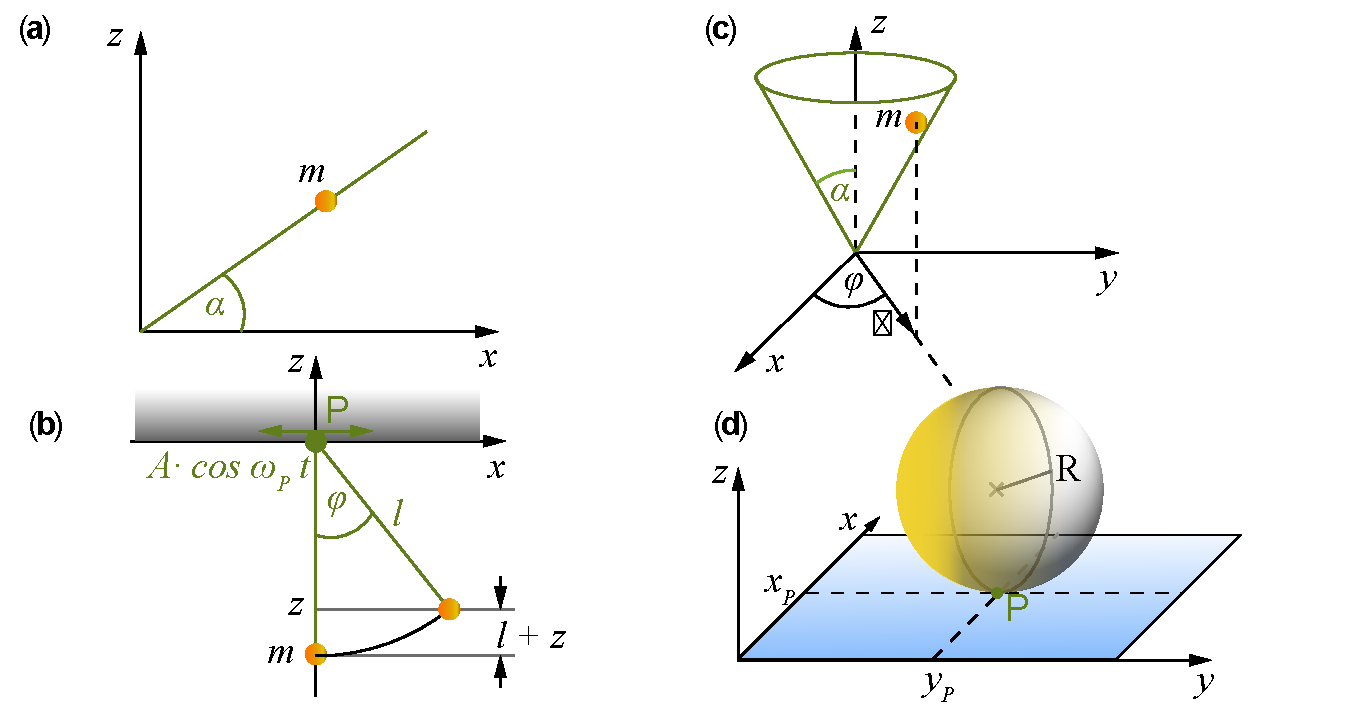
\includegraphics[width=\columnwidth]{ZwangsbedingungenBsp.pdf}% 
\captionof{figure}{Beispiele f�r Zwangsbedingungen (siehe Beispiel \ref{bsp:bew_ZB}).} \label{abb:bew_ZwangBedBsp}
\end{center}
\label{bsp:bew_ZB}
\end{example}
%Ende BEISPIEL %%%%%%%%%%%%%%%%%%%%%%%%%%%%%%%%%%%%%%%%%%%%%%%%%%%%%%%%%%%%%%%%%%%%%%%%%%%%%%%%%%

\subsubsection{Lagrange-Gleichungen erster Art}\index{Lagrange-Gleichung!Erster Art} \label{kap:bew_Lagrange_I}

Wenn die $Z_B$ holonomen Zwangsbedingungen zu jedem Zeitpunkt $t$ in einem System erf�llt sein sollen, muss man die Newtonsche Bewegungsgleichung durch eine \emph{\gls{zwangskr}}\index{Zwangskr�fte} erweitern, denn offensichtlich kann nur eine solche Kraft, die \zb von einer Unterlage oder einem Faden vermittelt wird, die Zwangsbedingung erf�llen.
Diese Kraft ist anders als die eingepr�gte �u�ere Kraft \ia zun�chst unbekannt.
Wir betrachten vorerst einen einzelnen Massepunkt und k�nnen dann die holonomen Zwangsbedingungen geometrisch als Fl�chen interpretieren, auf denen sich der Massepunkt bewegen soll.
Dann muss die Zwangskraft senkrecht auf dieser Fl�che stehen, was allgemein $\vec{Z} \propto \gradv f$ bedeutet.
Wir k�nnen deshalb die Bewegungsgleichung um den Proportionalit�tsfaktor $\lambda$ erweitern, den wir \emph{\gls{lagrmult}} nennen.
Die Zwangskr�fte sind dann
\begin{align}
	\vec{Z}_k &= \sum\limits_{r=1}^{Z_B}\lambda_r \gradv_k f_r \quad\text{\bzw in Komponenten} ~~\nonumber \\
	Z_k &= \sum\limits_{r=1}^{Z_B}\lambda_r \frac{\partial {f_r}}{\partial {x_k}}\,. \label{eq:bew_Zwangskraefte}
\end{align}
Die Bewegungsgleichungen, jetzt wieder erweitert auf $N$ Teilchen \bzw $3N$ Koordinaten, lauten dann
\begin{subequations}
\begin{align}
	m_k \ddot{\vec{r}}_k &= \vec{F}_k + \sum\limits_{r=1}^{Z_B}\lambda_r \gradv_k f_r \qquad k = 1 \ldots N ~~~~\text{\bzw} \\
	m_i \ddot{x}_i &= F_i + \sum\limits_{r=1}^{Z_B}\lambda_r \frac{\partial {f_r}}{\partial {x_i}}\qquad  i = 1 \ldots 3N\,. 
\end{align} \label{eq:bew_Lagrange_I}
\end{subequations}

Die Gleichungen \eqref{eq:bew_Lagrange_I} hei�en Lagrange-Gleichungen erster Art und stellen ein System von $3N$ Bewegungsgleichungen dar, in welchem die $Z_B$ Zwangsbedingungen �ber die Lagrange-Multiplikatoren $\lambda_r$ implizit enthalten sind.
Wir wollen noch kurz ohne Beweis erw�hnen, dass bei Vorliegen holonomer Zwangsbedingungen folgende Beziehung f�r die Energie gilt \cite{Kuypers2012, Bartelmann2015}:
\begin{align}
	\frac{\D}{\D t} E = 	\frac{\D}{\D t} (T+U) = - \sum\limits_{k=1}^{Z_B}\lambda_r \frac{\partial f_r}{\partial t}\,.\label{eq:bew_Lagrange_IE}
\end{align}
F�r skleronome Zwangsbedingungen ($\partial f_r / \partial t = 0$) bleibt also die Energie des Systems konstant, die Zwangskr�fte leisten in diesem Fall keine Arbeit.\\
Die Frage ist nun, wie man die Lagrange-Gleichungen erster Art l�st. F�r holonome Zwangsbedingungen gibt es folgende \textit{L�sungsstrategie}, deren konkrete Umsetzung wir in den Beispielen \ref{bsp:bew_PerleDraht} und \ref{bsp:bew_Rollenpendel} zeigen: \\ \\
\smallskip
\fbox{\parbox{0.95\textwidth}{
\smallskip
\textbf{\textit{Allgemeine L�sungsstrategie f�r Lagrange-Gleichungen erster Art mit holonomen Zwangsbedingungen �ber die Methode der Lagrange-Multiplikatoren}}
\begin{enumerate}
    \item Man stellt die Bewegungsgleichungen
      \eqref{eq:bew_Lagrange_I} und die Zwangsbedingungen
      $f_r(x_i,t)=0$ f�r die $3N$ Koordinaten $x_i$
      der $N$ Massepunkte auf.
    \item Man berechnet aus den Zwangsbedingungen die ersten und zweiten Ableitungen
      von $f_r(x_i,t)=0$:
      \begin{align}
         \dot{f}_r &= \sum\limits_{i=1}^{3N} \lambda_r \frac{\partial {f_r}}{\partial {x_i}} \dot{x}_i  + \frac{\partial {f_r}}{\partial t} \nonumber \\
        \ddot{f}_r &= \sum\limits_{i=1}^{3N} \lambda_r \frac{\partial {f_r}}{\partial {x_i}} \ddot{x}_i - a_r(t,x, \dot{x}) = 0\,.  \label{eq:bew_Lagrange_Ia}
      \end{align}
      Der Term $a_r(t,x, \dot{x})$ enth�lt alle Ableitungen
      von $f_r$ nach $t, x_i$ und $\dot{x}_i$, h�ngt aber nicht
      von den zweiten Ableitungen $\ddot{x}_i$ ab.
    \item Man setzt f�r die $\ddot{x}_i$
      in \eqref{eq:bew_Lagrange_Ia} die Bewegungsgleichungen \eqref{eq:bew_Lagrange_I} ein
      und erh�lt ein lineares inhomogenes Gleichungssystem
      f�r die $Z_B$ Lagrange-Multiplikatoren $\lambda_r$,
      welche in der impliziten Form 
      \begin{align}
          \lambda_r = \lambda_r(t, x, \dot{x})\,,\quad r = 1 \ldots Z_B \label{eq:bew_Lagrange_Ib}
      \end{align}
      berechnet werden k�nnen.
    \item Man setzt die impliziten Lagrange-Multiplikatore L�sungen \eqref{eq:bew_Lagrange_Ib} in die
      Bewegungsgleichungen \eqref{eq:bew_Lagrange_I} ein
      und erh�lt schlie�lich ein $3N$-dimensionales
      Differentialgleichungssystem zweiter Ordnung
      \begin{align}
	m_i \ddot{x}_i &= F_i + \sum\limits_{r=1}^{Z_B}\lambda_r(t, x, \dot{x}) \frac{\partial f_r}{\partial x_i}\,, \label{eq:bew_Lagrange_Ic}
      \end{align}
      das mit den �blichen Methoden zur L�sung von
      Differentialgleichungen (DGL)\index{Differentialgleichung}
      gel�st werden kann. 
    \item Mit den L�sungen kann man dann auch
      die Lagrange-Multiplikatoren und damit �ber
      \eqref{eq:bew_Zwangskraefte} die Zwangskr�fte berechnen,
      falls man diese explizit braucht.
      Zu beachten ist noch, dass alle Anfangsbedingungen
      den Zwangsbedingungen gen�gen m�ssen.\footnotemark
    \item F�r nicht-holonome Zwangsbedingungen gibt es kein allgemein g�ltiges Vorgehen. Wenn die nicht-holonomen Zwangsbedingungen in differentieller Form vorliegen, kann man die dargestellte Methode in leicht abgewandelter Form ebenfalls verwenden. 
		\item Wir werden die Methode der Lagrange-Multiplikatoren \zb in
 \probref{bew_unwucht}, \probref{bew_Trebuchet} \ua anwenden.
\end{enumerate}
}} 

\subsubsection{Verallgemeinerte Koordinaten}\label{kap:bew_general_coordinates}

In den (holonomen) Zwangsbedingungen \eqref{eq:bew_holonome_ZB} und den Lagrange-Gleichungen erster Art \eqref{eq:bew_Lagrange_I} haben wir zun�chst noch kartesische \bzw orthonormale Koordinaten (\zb Kugelkoordinaten) angenommen.
Deswegen mussten wir $3 N$ Komponentengleichungen l�sen und dabei $Z_B$ Zwangsbedingungen ber�cksichtigen.
Wir k�nnen uns die Aufgabe vereinfachen, indem wir zu sogenannten \emph{verallgemeinerten} oder \emph{generalisierten}\glslink{genkoord}{} Koordinaten \glslink{genkoord} �bergehen.
Diese Koordinaten $q_j$ werden als unabh�ngige Parameter entsprechend der Anzahl der \emph{Freiheitsgrade}\index{Freiheitsgrad} $F$ definiert und sind dann nicht mehr per Definition weiter durch Zwangsbedingungen eingeschr�nkt, da diese ja durch die entsprechende Auswahl der $q_j$ bereits ber�cksichtigt worden sind.
F�r holonome Zwangsbedingungen existiert dann folgende Beziehung:
\begin{align}
	x_i=x_i(t, q_j) \qquad i = 1\ldots 3N \quad j = 1 \ldots F\,. \label{eq:general_coordinates}
\end{align}
Diese verallgemeinerten Koordinaten k�nnen die Behandlung vieler Probleme der Mechanik (und auch anderer Themengebiete) deutlich vereinfachen, insbesondere dann, wenn man nicht an den Zwangskr�ften interessiert ist. 

\subsubsection{Lagrange-Gleichungen zweiter Art}\index{Lagrange-Gleichung!Zweiter Art} \label{kap:bew_Lagrange_II}

Wir beginnen mit \eqref{eq:general_coordinates}.
Die Zwangsbedingungen sind entsprechend der Bedingung
\begin{align}
	\frac{\partial{f_r}}{\partial{q_j}} = \sum\limits_{i}^{3N} \frac{\partial{f_r}}{\partial{x_i}} \frac{\partial{x_i}}{\partial{q_j}} \stackrel{!}{=} 0 \label{kap:bew_Zwangsbedingung_II}
\end{align}
ber�cksichtigt, denn wenn die Zwangsbedingungen von den $q_j$ abhingen, st�nde das im Widerspruch zur Definition der verallgemeinerten Koordinaten.
Multipliziert man die Lagrange-Gleichung erster Art mit ${\partial{x_i}}/{\partial{q_j}}$ erh�lt man:
\begin{align}
	\sum\limits_{i}^{3 N} m_i \ddot{x}_i \frac{\partial{x_i}}{\partial{q_j}} &= \sum\limits_{i}^{3 N} F_i \frac{\partial{x_i}}{\partial{q_j}} + \sum\limits_{r=1}^{Z_B}\lambda_r \sum\limits_{i}^{3N} \frac{\partial {f_r}}{\partial {x_i}} \frac{\partial {x_i}}{\partial {q_j}}\,. \label{eq:bew_Lagrange_II_a}
\end{align}
Der erste Term 
\begin{align}
	Q_j &= \sum\limits_{i}^{3N} F_i \frac{\partial {x_i}}{\partial {q_j}} \label{eq:bew_Lagrange_II_b}
\end{align}
ist offensichtlich eine Kraft und wird verallgemeinerte oder \emph{generalisierte Kraft}\index{Kraft!generalisierte}\index{Kraft!verallgemeinerte} genannt, w�hrend der zweite Term aufgrund der Bedingungen f�r die verallgemeinerten Koordinaten verschwindet.
Durch geeignete Umformung wie Vertauschung der partiellen Ableitungen und Einf�hrung \emph{generalisierter Geschwindigkeiten} $\dot{q}_j$ und der kinetischen Energie $T$
\begin{align}
	\dot{q}_j &= \frac{\D}{\D t} q_j\,, \quad T= \frac{1}{2} \sum\limits_{i}^{3N} m_i \dot{x}_i^2 \label{eq:bew_Lagrange_II_c}
\end{align}
erh�lt man nach einfachen Rechnungen (siehe \cite{Greiner2004, Bartelmann2015, Kuypers2012}) die \emph{Lagrange-Gleichungen zweiter Art}:
\begin{align}
	\frac{\D}{\D t} \frac{\partial T}{\partial \dot{q}_j} - \frac{\partial T}{\partial q_j} = Q_j \qquad j = 1 \ldots F\,. \label{eq:bew_Lagrange_II_d}
\end{align}
Die $Q_j$ sind zun�chst noch beliebige Kr�fte, sie k�nnen konservativ oder auch dissipativ sein.
Deshalb zerlegen wir diese in
	\[Q_j = Q_j^\text{(kons)} + Q_j^\text{(diss)}\,.
\]
Wir nehmen zun�chst nur konservative Kr�fte an und k�nnen dann schreiben:
	\[Q_j = Q_j^\text{(kons)} = \sum\limits_{i}^{3N} F_i \frac{\partial {x_i}}{\partial {q_j}} = -  \frac{\partial {U(t,x)}}{\partial {q_j}}\,,
\]
woraus schlie�lich mit der \emph{\gls{lagrfkt}} $\mathcal{L} = T -U $\index{Lagrange-Funktion|textbf} die Lagrange-Gleichungen zweiter Art f�r konservative Kr�fte folgen:
\begin{align}
	\mathcal{L} &= T - U = T(t, q_j, \dot{q}_j) - U(t, q_j) \nonumber \\
		\frac{\D}{\D t} \frac{\partial \mathcal{L}}{\partial \dot{q}_j} - \frac{\partial \mathcal{L}}{\partial q_j} &=  \left\{\frac{\D}{\D t} \frac{\partial }{\partial \dot{q}_j} - \frac{\partial}{\partial q_j} \right\} \mathcal{L} = 0 \qquad j = 1 \ldots F\,. \label{eq:bew_LagrangeGl_II}
\end{align}
Die Lagrange-Gleichungen sind $F$ Differentialgleichungen zweiter Ordnung f�r die $q_j(t)$.
Die allgemeine L�sung hat demnach demnach $2F$ Parameter \bzw Anfangsbedingungen.\\
W�hrend die Newtonschen Bewegungsgleichungen f�r kartesische Koordinaten formuliert wurden und relativ kompliziert auf andere Koordinatensysteme zu transformieren sind, ist der Lagrange-Formalismus koordinatenunabh�ngig.
Die generalisierten Koordinaten sind frei w�hlbar, solange sie den Zwangsbedingungen gen�gen.
Man kann also mit den Lagrange-Gleichungen zweiter Art die Bewegungsgleichungen direkt in nicht-kartesischen Koordinaten aufstellen, die Lagrange-Gleichungen zweiter Art sind \emph{forminvariant}\glslink{forminvar}.
Forminvarianz bedeutet, dass die Lagrange-Gleichungen zweiter Art beim �bergang von Koordinaten $q_j$ zu neuen Koordinaten $Q_j(t, q)$ in ihrer Form erhalten bleiben:
\begin{align*}
	q_j \rightarrow Q_j(t, q) \quad&\text{und} \quad \mathcal{L}(q_j, \dot{q}_j, t) \rightarrow \mathcal{L'}(Q_j, \dot{Q}_j, t) \\
				\frac{\D}{\D t} \frac{\partial \mathcal{L}}{\partial \dot{q}_j} - \frac{\partial \mathcal{L}}{\partial q_j} &= 0 \rightarrow  \frac{\D}{\D t} \frac{\partial \mathcal{L'}}{\partial \dot{Q}_j} - \frac{\partial \mathcal{L'}}{\partial Q_j}  = 0 \qquad j = 1 \ldots F\,.
\end{align*}
Diese Eigenschaft ist �u�erst vorteilhaft, wenn man Probleme in nicht-kartesischen Koordinatensystemen oder in Nicht-Inertialsystemen behandeln will (\probref{bew_LagrangeII_a}).

Wir f�hren jetzt noch den \emph{kanonischen} oder \emph{generalisierten Impuls}\index{Impuls!kanonischer} ein:
\begin{align}
	p_j = \frac{\partial \mathcal{L}}{\partial \dot{q}_j}\,.\label{eq:bew_Lagrange_II_f}
\end{align}
Wenn die Lagrange-Funktion\index{Lagrange-Funktion} $\mathcal{L}$ nicht von $q_j$ abh�ngt, dann ist der zugeh�rige kanonische Impuls $p_j$ eine Erhaltungsgr��e und die zugeh�rige Koordinate ist eine \emph{zyklische} Koordinate\glslink{zykkoord}.
Es ist bei Problemen oft vorteilhaft, gezielt nach zyklischen Koordinaten zu suchen, da die Erhaltungsgr��e $p_j = \text{const}$ einer ersten Integration der Bewegungsgleichung entspricht.
So f�hrt die zyklische Koordinate $q_j$, die dem Drehwinkel um eine feste Achse entspricht, auf die Erhaltung des Drehimpulses, \vgl dazu auch \kap{bew_ZKP_NZKF}.\\
Bevor wir auf L�sungsstrategien f�r die Lagrange-Gleichungen zweiter Art eingehen, wollen wir noch eine Betrachtung zur Energieerhaltung machen.
Wir definieren zun�chst die \emph{Hamilton\indexp{Hamilton, Sir William Rowan}\footnote{Sir William Rowan Hamilton (1805--1865) war ein irischer Mathematiker und Physiker und Royal Astronomer f�r Irland. 1835 gelang ihm eine Formulierung der Mechanik, die heute seinen Namen tr�gt und die fast 100 Jahre sp�ter wegweisend f�r den �bergang zur Quantenmechanik war. Im Rahmen dieses Buches k�nnen wir auf diese leider nicht eingehen. Wir verweisen auf die Literatur (\zb \cite{Simonyi2004, Greiner2004, Bartelmann2015, Kuypers2012}).}-Funktion}\index{Hamilton-Funktion}
\begin{align}
	\mathcal{H} = \sum\limits_{i} \dot{q}_i \frac{\partial \mathcal{L}}{\partial \dot{q}_i} -  \mathcal{L} =  \sum\limits_{i} p_i \dot{q}_i - \mathcal{L}\,. \label{eq:bew_Hamilton_Fkt}
\end{align}
Wie man leicht nachrechnen kann, ist f�r konservative Systeme,
geschwindigkeitsunabh�ngige \pot{}e und skleronome Zwangsbedingungen
die Hamilton-Funktion gleich der Gesamtenergie $E$ des Systems,
weswegen f�r die Gesamtenergie eines Systems oft auch das Symbol
$H$ verwendet wird.%
\footnote{Wir werden auch in der Himmelsmechanik (Band II, Kapitel 3) der allgemeinen (historischen) Konvention folgend f�r die Gesamtenergie $H$ benutzen.}
Wir wollen nun auch f�r Lagrange-Gleichungen zweiter Art eine \textit{L�sungsstrategie} aufzeigen.
Diese gilt f�r holonome Zwangsbedingungen und konservative Kraftfelder.
In den Beispielen \ref{bsp:bew_PerleDraht} und \ref{bsp:bew_Rollenpendel} zeigen wir das Vorgehen wiederum konkret.\\
~

\fbox{\parbox{0.95\textwidth}{
\medskip
\textbf{\textit{L�sungsstrategie f�r Lagrange-Gleichungen zweiter Art}}
\begin{enumerate}
	\item Man �berlegt sich die aus den $Z_B$ holonomen Zwangsbedingungen verbleibenden $F = 3 N - Z_B $ Freiheitsgrade des Systems und ordnet jedem Freiheitsgrad eine generalisierte Koordinate $q_j$ zu.
          Die explizite Form der Zwangsbedingungen $f_r(x_i,t)=0$ muss nicht unbedingt bekannt sein.
	\item Man �berpr�ft, dass die $q_j$ nicht durch Zwangsbedingungen eingeschr�nkt sind.
          Zwischen den kartesischen Koordinaten $x_i$ und den $q_j$ besteht folgender Zusammenhang:
		\[x_i =  x_i(t, q_1,q_2,\ldots, q_{F})\,.
	\]
	\item Man schreibt die Lagrange-Funktion $\mathcal{L} = T - U$ auf.
	\item Man sucht nach zyklischen Koordinaten.
          Die damit verbundenen Impulse $p_j$ sind Erhaltungsgr��en und damit erste Integrale der Bewegungsgleichungen.
	\item F�r die nichtzyklischen Koordinaten stelle man mit den Lagrange-Gleichungen zweiter Art \eqref{eq:bew_LagrangeGl_II} die Bewegungsgleichungen auf, die wiederum mit den �blichen Methoden (analytisch \bzw numerisch) zur L�sung von Differentialgleichungen gel�st werden k�nnen (siehe \kap{bew_einschub_DGL}). 
\end{enumerate}
}}
\medskip

\subsubsection{Lagrange-Gleichungen zweiter Art mit Reibung und externen Kr�ften}\label{kap:bew_Lagrange_II_R}


\subparagraph{Generalisierte externe Kr�fte}

Bisher hatten wir bei der Herleitung der Lagrange-Gleichungen zweiter Art ausschlie�lich konservative Kr�fte betrachtet und konnten damit die Kr�fte allein durch die potentielle Energie $U$ beschreiben. Um auch nicht-konservative Kr�fte im Lagrange-Formalismus ber�cksichtigen zu k�nnen, werden die Kr�fte in die jeweilige Richtung der generalisierten Koordinaten \glq{}projiziert\grq. Diese Kr�fte hatten wir schon als generalisierte Kr�fte \eqref{eq:bew_Lagrange_II_b} eingef�hrt:
\begin{align}
	  Q_j &= \sum\limits_{i}^{3N} F_i \frac{\partial {x_i}}{\partial {q_j}}\,. \label{eq:bew_gen_Kraft_neu}
\end{align}


\subparagraph{Dissipationsfunktion}

Die dissipativen Kr�fte (also Kr�fte, die dem System Energie entziehen) k�nnen ebenfalls als generalisierte Kraft im Lagrange-Formalismus ber�cksichtigt werden. Alternativ kann man eine \emph{Dissipationsfunktion} $U_\text{R}$ einf�hren. Wir starten dazu von den generalisierten Reibungskr�ften\index{Reibungskr�fte!generalisierte} $F_{\text{R}j}$, die sich gem�� \eqref{eq:bew_Lagrange_II_b} \bzw \eqref{eq:bew_gen_Kraft_neu} �ber 
\begin{align}
	F_{\text{R}j} = \sum\limits_{k=1}^{N} \vec{F}_{\text{R}k} \cdot \frac{\partial \vec{r}_k}{\partial q_j} \label{eq:bew_gen_Reibungskraft}
\end{align}
aus den kartesischen Reibungskr�ften berechnen lassen. 
Wir hatten in \kap{bew_newton_axioms} gesehen, dass in der Mechanik vielfach die Reibungskraft proportional zur Geschwindigkeit ist, sodass $\vec{F}_{\text{R}k} = - \beta_k(v_k) \vec{v}_k/v_k$ gilt.
F�r solche Kr�fte kann ein \emph{Dissipations\potsuf{}}\index{Dissipationspotential}\index{Potential!Dissipationspotential} (auch Dissipationsfunktion\index{Dissipationsfunktion} genannt) definiert werden:
\begin{align}
	U_\text{R} &= \sum\limits_{k=1}^{N} \int\limits_{0}^{v_k} \beta_k(v_k') \:\D v_k' ~~~~\rightarrow~~~ F_{\text{R}j} = - \frac{\partial U_\text{R}}{\partial \dot{q}_j}\,.\label{eq:bew_Dissipationspotential}
\end{align}
Die negativen partiellen Ableitungen der Dissipationsfunktion nach den generalisierten Geschwindigkeiten m�ssen nat�rlich wieder die generalisierten Kr�fte der dissipativen Kr�fte ergeben.

Verallgemeinert berechnet sich das Dissipationspotential f�r die verschiedenen Reibungsarten nach:
\begin{itemize}
    \item \textit{Gleitreibung}: $U_{\text{R}_1} = \mu\,F_\text{N}\,|\vec{v}_\text{rel}|^1$,\,mit $\mu$ als Gleitreibungskoeffizient, $F_\text{N}$ ist die Normalkraft,
    \item \textit{Stokes-Reibung}\index{Stokes-Reibung}\index{Reibung!Stokes-}: $U_{\text{R}_2} = \frac{1}{2}\,\eta\,|\vec{v}_\text{rel}|^2$,\,mit $\eta$ als D�mpfungskonstante,
    \item \textit{Newton-Reibung} (\zb Luftwiderstand): $U_{\text{R}_3} = \frac{1}{3}\,c_w\,|\vec{v}_\text{rel}|^3$,\, mit $c_w$ als Luftwiderstandsbeiwert.
\end{itemize}

Damit lauten bei Vorliegen externer (nicht-konservativer) Kr�fte und eines Dissipations\potsuf{}s die Lagrange-Gleichungen zweiter Art:
\begin{align}
			&\frac{\D}{\D t} \frac{\partial \mathcal{L}}{\partial \dot{q}_j} &- \frac{\partial \mathcal{L}}{\partial q_j} + \frac{\partial U_\text{R}}{\partial \dot{q}_j} = Q_\text{j} ~~~~j= 1, \ldots, F\\
    &\text{Hierin sind f�r ein System mit}~~ F ~~\text{Freiheitsgeraden:} \notag \\
    q_j~~~&\text{die generalisierte Koordinaten,} \notag\\
		\dot{q}_j~~~&\text{die generalisierte Geschwindigkeiten,}\notag \\
    U_\text{R}~~~&\text{die Dissipationsfunktion und }\notag \\
		Q_j~~~&\text{die generalisierte Kr�fte}.\notag
\end{align} \label{eq:bew_LagrangeGl_II_Reibung}

\subsubsection{Anwendung des Lagrange-Formalismus auf Schwingungen}\index{Schwingung} \label{kap:bew_schwingung}

Schwingungen sind Bewegungen um eine Gleichgewichtslage herum.
Sie sind extrem wichtig in der Physik und besonders die harmonischen Schwingungen waren von grundlegender Bedeutung in der Weiterentwicklung der klassischen Mechanik hin zur Quantenmechanik.  Da sich fast alle Kr�fte lokal linearisieren lassen, spielen harmonische Schwingungen beispielsweise in der Akustik, der Festk�rper- und Quantenphysik und auch der Spektroskopie eine gro�e Rolle. 
Wir wollen uns zun�chst auf Schwingungen mit einem Freiheitsgrad beschr�nken.
Der Lagrange-Formalismus l�sst sich hierbei vorteilhaft anwenden.
Wir werden diesen dann auch auf mehrere Freiheitsgrade und Systeme von mehreren schwingenden Massepunkten erweitern.
In diesem Zusammenhang werden wir annehmen, dass alle Teilchen nur unter der Wirkung rein konservativer Kr�fte liegen.\\
Dabei gehen wir direkt zu einer generalisierten Koordinate $q$ �ber und untersuchen nun die spezielle Situation, dass der Ort $q$ des Teilchens nur wenig von einer stabilen Gleichgewichtslage $q_0$ abweicht.
\emph{Gleichgewicht}\index{Gleichgewicht} in der Position $q_0$ bedeutet, dass dort die Summe aller auf den Massepunkt wirkenden (generalisierten) Kr�fte gleich Null ist.
\emph{Stabilit�t}\index{Stabilit�t} bedeutet, dass f�r kleine Auslenkungen $q-q_0$ und geringe Impulse r�cktreibende Kr�fte wirken, die ein unbegrenztes Anwachsen der Auslenkung verhindern.
\begin{align*}
	F = -\frac{\partial U}{\partial x} 
\end{align*}
Das \pot{} kann im Allgemeinen eine beliebige Gestalt annehmen.
In vielen F�llen besitzt das \pot{} jedoch ein lokales Minimum bei $q_0$ (dem Ort der Gleichgewichtslage).
Wir entwickeln daher das \potz{} um das Minimum bei $q_0$ und erhalten:
\begin{align}
	U = U(q_0) + \frac{\d U}{\d q}\bigg|_{q_0}\cdot(q-q_0) + \frac{1}{2} \frac{\d^2 U}{\d q^2}\bigg|_{q_0}\cdot(q-q_0)^2 + \sum\limits_{k=3}^\infty \frac{1}{k!} \frac{\d^k U}{\d q^k}\bigg|_{q_0}\cdot(q-q_0)^k \label{eq:bew_Schwingung_a}
\end{align}
Als konstanter Wert des \potz{}s ist der erste Term irrelevant,
Der zweite Term ist Null, da das \potz{} um sein Minimum entwickelt wurde.
In vielen Anwendungen spielt bei kleinen Auslenkungen nur der quadratische Term in $q$ eine Rolle,  alle weiteren Terme werden ignoriert.
Dies f�hrt auf das \pot{} einer \emph{harmonischen} Schwingung\index{Schwingung!harmonische}.
Bei gr��eren Auslenkungen muss das \potz{} mit weiteren Termen der Entwicklung \eqref{eq:bew_Schwingung_a} ber�cksichtigt werden, was auf \emph{anharmonische	}\index{Schwingung!harmonische} Schwingungen f�hrt.\\
F�r die Aufstellung der Lagrange-Funktion ben�tigen wir noch die kinetische Energie, die definiert ist als
\begin{align*}
T &= \frac{1}{2}m \sum\limits_{i}^{3}{\dot{x}_i{}}^2 = \frac{1}{2} m \sum\limits_{i}^{3}\ \lk \sum\limits_{j}^{F} \frac{\partial x_i}{\partial q_j} \dot{q} \rk ^2 \,.
\end{align*}
F�r eindimensionale Bewegungen mit nur einer generalisierten Koordinate hei�t das:
\begin{align*}
	T &= \frac{1}{2}m \dot{x}^2 = \frac{1}{2} m \,  \dot{q}^2 \lk \frac{\partial x}{\partial q}\rk^2 =\: \frac{1}{2} m \,\dot{q}^2 \,h(q) \,.
\end{align*}
Den Ausdruck $h(q) = \lk\frac{\partial x}{\partial q}\rk ^2$ kann man ebenfalls um $q_0$ entwickeln und erh�lt
\begin{align}
	 T(q,\dot{q}) = \frac{m \dot{q}^2}{2} \lek h(q_0) + \sum\limits_{k=1}^\infty \frac{1}{k!} \frac{\d^k h(q)}{\d q^k}\bigg|_{q_0}\,(q-q_0)^k  \rek \,. \label{eq:bew_Schwingung_b}
\end{align}
Da der Vorfaktor bereits von zweiter Ordnung in $\dot{q}$ ist, muss bei geringen Auslenkungen in der Reihenentwicklung von $h(q)$ nur der konstante Beitrag ber�cksichtigt werden, vorausgesetzt $\dot{q}$ und $q$ sind von der gleichen Gr��enordnung, was bei kleinen Schwingungsamplituden der Fall ist.
Im diesem Grenzfall lautet die Lagrange-Funktion
\begin{align}
\mathcal{L} = T(q,\dot{q}) - U(q) = \frac{\tilde{m}}{2}\dot{q}^2 - \frac{1}{2} \frac{\partial^2 U}{\partial q^2}\bigg|_{q_0}\, q^2 \,,\label{eq:bew_Schwingung_c}
\end{align}
wobei wir $\tilde{m} = h(q_0) m$ benutzt haben.
Das ist die Schwingungsgleichung f�r eine harmonische Schwingung wie beim Federpendel, was unmittelbar einsichtig ist, wenn man $x=q$ setzt. \\

F�r anharmonische Schwingungen\index{Schwingung!anharmonische} ergibt sich die Lagrange-Funktion aus der Mitnahme weiterer Terme von \eqref{eq:bew_Schwingung_a} und \eqref{eq:bew_Schwingung_b}.
Wenn wir ein symmetrisches \pot{} um $q_0$ annehmen, gilt in der n�chsten N�herung:
\begin{align}
	\mathcal{L} = T - U & = \frac{m}{2}\dot{q}^2 \lek h(q_0) + (q-q_0) \frac{\d h(q)}{\d q}\bigg|_{q_0} + \frac{1}{2} \,(q-q_0)^2 \frac{\d^2 h(q)}{\d q^2}\bigg|_{q_0} \rek \nonumber \\
	          & \quad - \frac{1}{2} (q-q_0)^2 \lek \frac{\d^2 U}{\d q^2}\bigg|_{q_0}  -  \frac{1}{12} \frac{\d^4 U}{\d q^4}\bigg|_{q_0}\, (q-q_0)^2 \rek \,. \label{eq:bew_Schwingung_d}
\end{align}
Die aus \eqref{eq:bew_Schwingung_c} �ber die Lagrange-Gleichungen abgeleitete Schwingungsgleichung\footnote{Dies ist eine lineare Differentialgleichung mit konstanten Koeffizienten, weswegen man auch den N�herungs�bergang zu \eqref{eq:bew_Schwingung_c} auch als Linearisierung\index{Linearisierung} bezeichnet.} f�r die generalisierte Koordinate im Grenzfall geringer Schwingungen lautet
\begin{align}
	  \ddot{q} + \omega_0^2 \,q \:=\: 0 \,. \label{eq:bew_Schwingung01a}
\end{align}
F�r beliebig starke Schwingungen gilt allgemein:
\begin{align}
	  m \frac{\D}{\D t}\lk h(q) \,\dot{q} \rk - \frac{m \dot{q}^2}{2} \frac{\d h}{\d q} + \frac{\d U}{\d q} = 0 \,, \label{eq:bew_Schwingung01b}
\end{align}
worin $ h(q)$ eine Funktion allein von $q$ ist, die sich gem�� \eqref{eq:bew_Schwingung_b} berechnen l�sst.

\subparagraph{\textbf{Schwingungen und Dissipation}} 

In vielen Anwendungen treten bei Schwingungen dissipative Kr�fte auf, die zu einer D�mpfung der Schwingung f�hren.
Wir wollen den Einfluss einer solchen D�mpfung im Folgenden mit ber�cksichtigen und dabei zun�chst annehmen, dass die generalisierte dissipative Kraft linear in $\dot{q}_j$ ist, was \zb f�r die Stokes-Reibung \eqref{eq:bew_StokesReibung} gilt.
Wir k�nnten im Lagrange-Formalismus starten und das generalisierte \pot{} der Reibung berechnen.
Der Einfachheit halber gehen wir aber direkt von den Bewegungsgleichungen \eqref{eq:bew_Schwingung01a} \bzw \eqref{eq:bew_Schwingung01b} aus und addieren eine in $\dot{q}_j$ lineare Reibungskraft:
\begin{align}
	\ddot{q} + \beta \dot{q} + \omega_0^2 \,q \:=\: 0 \,.\label{eq:bew_Schwingung02}
\end{align}
Dieser lineare Fall ist in vielen F�llen eine gute Beschreibung der Realit�t. 
Bei \eqref{eq:bew_Schwingung02} handelt es sich ebenfalls um eine gew�hnliche lineare homogene DGL zweiter Ordnung.
F�r derartige Probleme kann man den von Euler gefundenen Exponentialansatz mit komplexen Zahlen 
\begin{align}
	Q(t) = \mathrm{e}^{\mathrm{i} \omega t} \label{eq:bew_Schwingung03}
\end{align}
verwenden und die allgemeine L�sung rasch erhalten: 
\begin{align}
  \lk -\omega^2 + \mathrm{i} \beta \omega + \omega_0^2 \rk \mathrm{e}^{\mathrm{i} \omega t}\,. \label{eq:bew_Schwingung04}
\end{align}
Die Bewegungsgleichung kann nur erf�llt werden, wenn der Term in der Klammer verschwindet.
Reibungsterme, die quadratisch in $\dot{q}_j$ sind, machen die mathematische Behandlung wesentlich anspruchsvoller, da die Bewegungsgleichung dann nicht mehr linear ist.
In der Regel werden wir diese dann numerisch l�sen m�ssen.


\subsubsection{Vergleichende Darstellung der L�sung der Bewegungsgleichung nach den Lagrange-Gleichungen erster und zweiter Art} \label{kap:bew_Lagrange_GlIV}

Wir wollen im Folgenden zwei instruktive Beispiele zur Anwendung der Lagrange-Gleichungen erster und zweiter Art zeigen.
Die Beispiele folgen den in den Kapiteln \ref{kap:bew_Lagrange_I} und \ref{kap:bew_Lagrange_II} gezeigten L�sungsstrategien und dienen als guter Einstieg in die �bungen.

\begin{figure}
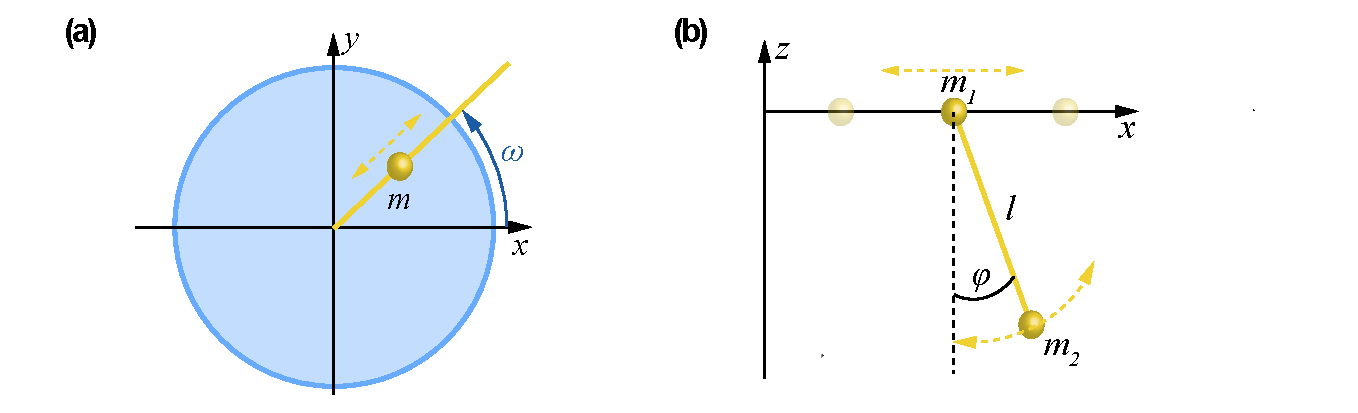
\includegraphics[width=\columnwidth]{RollenPendel.pdf}% 
\caption[Beispiele zum Lagrange-Formalismus.] {Beispiele zum Lagrange-Formalismus. \fa Rotierende Scheibe mit gleitender Perle auf Draht und \fb Rollenpendel.}
\label{abb:bew_Rollenpendel}
\end{figure}

\subparagraph{\textbf{Rotierende Scheibe mit gleitender Perle auf Draht}} 

Als erstes Beispiel wollen wir anhand eines Standardbeispiels aus vielen Lehrb�chern den Vergleich der beiden Methoden darstellen.
Wir haben hier ein Problem eines einzelnen Massepunktes unter Zwangskr�ften und Scheinkr�ften, da ein Nicht-Inertialsystem vorliegt (siehe \figref{bew_Rollenpendel}a). 

%BEISPIEL %%%%%%%%%%%%%%%%%%%%%%%%%%%%%%%%%%%%%%%%%%%%%%%%%%%%%%%%%%%%%%%%%%%%%%%%%%%%%%%%%%
\begin{example}{Zwangsbedingungen - Beispiel rotierende Scheibe mit gleitender Perle auf Draht}
\smallskip
\begin{itemize}
	\item \emph{L�sung mittels der Lagrange-Gleichungen erster Art}\\
	Wir betrachten nur die $x$-$y$-Ebene und verwenden Polarkoordinaten (Zylinderkoordinaten mit $z=0$).
        Dann gibt es nur eine Zwangsbedingung und nur einen Lagrange-Multiplikator $\lambda$:
			\[ f_1(\varphi) = \varphi - \omega t = 0 \]
Die Lagrange-Gleichung erster Art lautet dann
	\[m \ddot{\vec{r}} = \lambda \: \gradv f\,.
\]
Mit den Beziehungen f�r die Beschleunigung und den Gradienten f�r Zylinderkoordinaten k�nnen wir schreiben
\begin{align}
		m \lk \ddot{\varrho} - \varrho \dot{\varphi}^2 \rk \vec{e}_\varrho + m \lk \varrho \ddot{\varphi} + 2 \dot{\varrho} \dot{\varphi} \rk \vec{e}_\varphi = \lambda \frac{\partial f}{\partial\varrho} \vec{e}_\varrho + \lambda\frac{1}{\varrho}\frac{\partial f}{\partial\varphi} \vec{e}_\varphi\,. \label{eq:bew_PerleDraht_1}
\end{align}
Da $\partial f/\partial\varrho = 0$, $\partial f/\partial\varphi = 1$ und $\ddot{f} = \ddot{\varphi} = 0$, folgen wegen der notwendigen Gleichheit der Koeffizienten vor den Einheitsvektoren in \eqref{eq:bew_PerleDraht_1}
\begin{align}
\lambda &= 2 m \varrho \dot{\varrho} \dot{\varphi}\,, \nonumber \\
m \lk \ddot{\varrho} - \varrho \dot{\varphi}^2 \rk &= 0 \quad \text{und} \quad m \varrho \ddot{\varphi} = 0\,.\label{eq:bew_PerleDraht_2}
\end{align}
Daraus ergibt sich wegen $\dot{f} = \dot{\varphi} - \omega = 0$ die Bewegungsgleichung f�r $\varrho$
	\[\ddot{\varrho} - \omega^2 \varrho = 0\,,
\]
deren L�sung 
\begin{align}
        \varrho (t) = A \mathrm{e}^{+\omega t} + B \mathrm{e}^{-\omega t} \label{eq:bew_PerleDraht_3}
\end{align}
lautet, wobei sich $A$ und $B$ aus den Anfangsbedingungen ergeben.
Die Perle wird sich f�r $A \neq 0$ also mit der Zeit zu immer gr��eren Radien bewegen.
Die Zwangskraft 
	\[\vec{Z} = \lambda \:\vec{\nabla} f = 2\: m \:\dot{\varrho}\: \omega \: \vec{e}_\varphi
\]
leistet wegen \eqref{eq:bew_Lagrange_IE} eine Arbeit von
	\[\frac{\partial T}{\partial t} = - \lambda \frac{\partial f}{\partial t} = 2\: m \varrho \dot{\varrho} \omega^2 
\]
am System.\\
	\item \emph{L�sung mittels der Lagrange-Gleichungen zweiter Art}\\
	Die Lagrange-Funktion hat wegen der Zwangsbedingung nur die generalisierte Koordinate $\varrho$ und lautet in Zylinderkoordinaten mit $z=0$
\begin{align}
		\mathcal{L} = T = \frac{m}{2} \lk \dot{\varrho}^2 + \varrho^2 \dot{\varphi}^2 \rk\,.\label{eq:bew_PerleDraht_4}
\end{align}
Die Lagrange-Gleichungen ergeben nat�rlich wieder \eqref{eq:bew_PerleDraht_2}.
Man sieht, wie einfach und elegant der Formalismus mit der Lagrange-Gleichung zweiter Art ist.
In \probref{bew_LagrangeII_b} werden wir das Problem noch etwas ausf�hrlicher untersuchen und auch auf F�lle mit Reibung und ver�nderlicher Drehzahl der Scheibe erweitern.
Auch sei hier darauf hingewiesen, dass die Energie des Systems nicht erhalten ist, denn die Zwangsbedingung ist ja skleronom, mithin leistet die Zwangskraft keine Arbeit.
\end{itemize}
\label{bsp:bew_PerleDraht}
\end{example}
%BEISPIEL %%%%%%%%%%%%%%%%%%%%%%%%%%%%%%%%%%%%%%%%%%%%%%%%%%%%%%%%%%%%%%%%%%%%%%%%%%%%%%%%%%

\subparagraph{\textbf{Rollenpendel}} 

Als zweites Beispiel wollen wir anhand eines weiteren Standardbeispiels aus den Lehrb�chern wiederum den Vergleich der beiden Methoden darstellen.
Das Rollenpendel (\figref{bew_Rollenpendel}b) besteht aus zwei gekoppelten Massepunkten.
Die Masse $m_1$ kann sich nur auf einer Schiene entlang der $x$-Achse (reibungsfrei) bewegen.
Die Masse $m_2$ ist starr �ber einen masselosen Stab mit der Masse $m_1$ verbunden und kann sich nur in der $x$-$z$-Ebene bewegen.
Es liegt hier also ein Problem eines Systems von zwei Massepunkten mit Zwangskr�ften (im Inertialsystem) vor. 

%BEISPIEL %%%%%%%%%%%%%%%%%%%%%%%%%%%%%%%%%%%%%%%%%%%%%%%%%%%%%%%%%%%%%%%%%%%%%%%%%%%%%%%%%%
\begin{example}{\textbf{Beispiel f�r Zwangsbedingungen - Das Rollenpendel}}
\smallskip
\begin{itemize}
	\item \emph{L�sung mittels der Lagrange-Gleichungen erster Art}\\ 
	Hier gehen wir einen leicht ver�nderten Weg, indem wir zur Herleitung der Bewegungsgleichungen die Lagrange-Funktion benutzen.
        Wir haben vier Koordinaten (in der $x$-$z$-Ebene) und zwei Zwangsbedingungen.
        Als Koordinaten f�r $m_1$ w�hlen wir $x_1, z_1$ und f�r $m_2$ sinnvollerweise die Polarkoordinaten $r, \varphi$.
        Dann gelten folgende Zwangsbedingungen und Beziehungen mit $l$ als fester Pendell�nge: 
		\[ f_1(x_1, z_1; r, \varphi) = z_1 = 0  \quad\text{und}\quad \frac{\partial f_1}{\partial z_1} = 1 \; , \]
		\[ f_2(x_1, z_1; r, \varphi) = r - l = 0 \quad\text{und}\quad \frac{\partial f_2}{\partial r} = 1 \; . \]
	Alle anderen Ableitungen von $f_r$ verschwinden.
        Wir bilden jetzt die Lagrange-Funktion $\mathcal{L}'(x_1,z_1,\dot{x}_1, \dot{z}_1,r, \varphi, \dot{r}, \dot{\varphi})$ und bestimmen aus dieser die Bewegungsgleichungen. 
		\[\mathcal{L}'= \frac{m_1}{2}\lk \dot{x}_1^2 +\dot{z}_1^2 \rk + \frac{m_2}{2}\lk \dot{x}_2^2 +\dot{z}_2^2 \rk - m_1 \:g\: z_1 \:- \:m_2 \:g \:z_2
	\]
	Die Lagrange-Funktion enth�lt noch keine Zwangsbedingungen.
        Wir brauchen noch die $x_2$ und $z_2$ als Funktionen von $r$ und $\varphi$.
        Man liest aus der \figref{bew_Rollenpendel}b mit $M = m_1 + m_2$ ab:
		\begin{align*}
		  x_2 &= x_1 + r \sin\varphi  ~~\rightarrow~~\dot{x}_2 = \dot{x}_1 + \dot{r} \sin\varphi + r \dot{\varphi} \cos\varphi \\
		  z_2 &= z_1 - r \cos\varphi  ~~\rightarrow~~\dot{z}_2 = \dot{z}_1 - \dot{r} \cos\varphi + r \dot{\varphi} \sin\varphi \\
			\rightarrow \mathcal{L}' &= \frac{M}{2} \lek \dot{x}_1^2 + \dot{z}_1^2 \rek  \\
						 &+ \frac{m_2}{2} \lek \dot{r}^2 + \dot{\varphi}^2 r^2 + 2 \dot{r} \lk \dot{x}_1 \sin\varphi - \dot{z}_1 \cos\varphi \rk + 2 r\dot{\varphi} \lk \dot{x}_1 \cos\varphi + \dot{z}_1 \sin\varphi \rk \rek \\
						 &- m_1 \:g\: z_1 - m_2 \:g \lk z_1 - r\cos\varphi \rk\,.
		\end{align*}
		Auf dem �blichen Weg �ber die Lagrange-Gleichungen zweiter Art
                bestimmt man die Bewegungsgleichungen, in die man
                erst jetzt die Zwangsbedingungen und die Lagrange-Multiplikatoren einsetzt,
                von denen nur f�r $z_1 (\lambda_1)$ und $r (\lambda_2)$
                die Parameter $\lambda_i$
                von 0 verschieden sind.
                Es ergeben sich dann vier Bewegungsgleichungen.
                Die Gleichungen f�r $\ddot{x}_1$ und $\ddot{\varphi}$ enthalten logischerweise keine Zwangskr�fte:
		\begin{align}
			&M \ddot{x}_1 + m_2 \: l \lk \ddot{\varphi} \cos\varphi \: - \dot{\varphi}^2 \sin\varphi \rk = 0\,, \label{eq:bew_RollPendel_1} \\
			&m_2 \: l \lk l\: \ddot{\varphi} +  \ddot{x}_1 \cos\varphi + g \sin\varphi \rk = 0\,. \label{eq:bew_RollPendel_2}
		\end{align}
Diese sind im Prinzip nach $x_1(t)$ und $\varphi(t)$ -- wenn auch nur numerisch -- aufl�sbar, wobei $x_1(t)$ eine zyklische Koordinate ist und f�r $\varphi(t)$ zur Berechnung der Energieerhaltungssatz benutzt werden kann, da ja holonome Zwangsbedingungen vorliegen.
Die beiden anderen Bewegungsgleichungen lauten
		\begin{align}
                  &m_2 \: l \lk \ddot{\varphi} \sin\varphi + \dot{\varphi}^2 \cos\varphi \rk + M \: g = \lambda_1 = Z_\text{Schiene}\text{ und}\label{eq:bew_RollPendel_3} \\
                  &m_2 \lk \ddot{x}_1 \sin\varphi - l \: \dot{\varphi}^2 - g \cos\varphi \rk = \lambda_2 = -Z_\text{Stange}\,. \label{eq:bew_RollPendel_4}
		\end{align}
Die beiden Zwangskr�fte sind aus den L�sungen f�r $x_1(t)$ und $\varphi(t)$ auch mit der Erweiterung f�r Reibungskr�fte berechenbar (\probref{bew_LagrangeII_b}).
Man kann noch, indem man \eqref{eq:bew_RollPendel_2} in \eqref{eq:bew_RollPendel_3} einsetzt, einen Zusammenhang zwischen der Auflagekraft auf der Schiene und der Zugkraft in der Stange herstellen,
	\[ Z_\text{Schiene} = m_1 \: g + Z_\text{Stange} \cos\varphi\,,
\]
was sofort einsichtig ist.
Wir werden gleich sehen, dass die Lagrange-Gleichungen zweiter Art viel einfacher zu handhaben sind.
Der Vollst�ndigkeit halber sei noch darauf hingewiesen, dass man nat�rlich die Bewegungsgleichungen \eqref{eq:bew_RollPendel_1}--\eqref{eq:bew_RollPendel_4} auch ohne die Lagrange-Funktion $\mathcal{L}'$ aufstellen kann.
Entsprechend \kap{bew_Lagrange_I} bildet man zun�chst die partiellen Ableitungen $\partial f_r/ \partial x_i$ sowie die zeitlichen Ableitungen der Zwangsbedingungen $\dot{f}_r$ und $\ddot{f}_r$ und berechnet die Lagrange-Multiplikatoren $\lambda_r(t, x_i, \dot{x}_i)$, die man in die Bewegungsgleichungen einsetzt.
Dem Leser ist dieses Vorgehen als �bung empfohlen.
	\item \emph{L�sung mittels der Lagrange-Gleichungen zweiter Art}\\
	Mit den Zwangsbedingungen $f_1(x_i, z_i) = z_1 = 0$ und $f_2(x_i, z_i) = (x_1 -x_2)^2 + z_2^2 - l^2 = 0 $ und den Beziehungen $ x_2 = x_1 + l\sin\varphi $ \bzw $ z_2 = l\cos\varphi$ schreiben wir die Lagrange-Funktion $\mathcal{L}$ in den generalisierten Koordinaten $q_1 = x_1$ und $q_2 = \varphi$ ($x$-$z$-Ebene) auf:
\begin{align*}
	T & = \frac{m_1}{2} \dot{x}_1^2  + \frac{m_2}{2} \lek \dot{x}_2^2 + \dot{z}_2^2 \rek \\
			& = \frac{M}{2} \dot{x}_1^2 + \frac{m_2}{2} \lk \dot{\varphi}^2 l^2 + 2 l\:\dot{x}_1 \dot{\varphi} \cos\varphi \rk \quad\text{und} \quad U = - m_2 \: g \: l \: \cos\varphi 
\end{align*}
\begin{align}
		\mathcal{L} &= T - U = \frac{M}{2} \dot{x}_1^2 + \frac{m_2}{2} \lk \dot{\varphi}^2 l^2 + 2 l \: \dot{x}_1 \dot{\varphi} \cos\varphi \rk + m_2 \: g \: l \cos\varphi \,.
\label{eq:bew_RollPendel_4a}
\end{align}
In $\mathcal{L}$ sind im Gegensatz zu $\mathcal{L}'$ beim Vorgehen nach der Lagrange-Gleichung erster Art die Zwangsbedingungen durch die entsprechende Verwendung der generalisierten Koordinaten bereits ber�cksichtigt.
Die Struktur von $\mathcal{L}$ zeigt bereits, dass es sich um ein verkoppeltes, und wie wir gleich noch deutlicher sehen werden, nichtlineares Problem handelt.
Wir suchen nach einer zyklischen Koordinate und finden wegen
\begin{align}
	\frac{\D}{\D t}\frac{\partial \mathcal{L}}{\partial \dot{x}_1} = \frac{\D}{\D t} \underbrace{\lek  M \dot{x}_1 + m_2 l \: \dot{\varphi} \cos\varphi \rek}_{P_\text{x}} = 0 \label{eq:bew_RollPendel_5}
\end{align}
$x_1$ als zyklische Koordinate, womit wir auch $P_\text{x}$ als den Gesamtimpuls bez�glich der $x$-Achse definieren k�nnen.
Damit haben wir auch ein erstes Bewegungsintegral gewonnen:
\begin{align}
	\dot{x}_1 = \frac{P_\text{x}}{M} - \frac{m_2}{M} l \: \dot{\varphi} \cos\varphi\,. \label{eq:bew_RollPendel_6}
\end{align}
Die zweite Lagrange-Gleichung bez�glich $\varphi$ ergibt:
\begin{align}
	l\:\ddot{\varphi} + g \sin\varphi + \ddot{x}_1 \cos\varphi = 0\,. \label{eq:bew_RollPendel_7}
\end{align}
Wir leiten \eqref{eq:bew_RollPendel_6} nach der Zeit ab, setzen das Ergebnis in \eqref{eq:bew_RollPendel_7} ein und erhalten schlie�lich:
\begin{align}
	\ddot{\varphi} \lk  1 - \frac{m_2}{M} \rk + \dot{\varphi}^2 \frac{m_2}{M} \sin\varphi \: \cos\varphi + \frac{g}{l} \sin\varphi = 0\,. \label{eq:bew_RollPendel_8}
\end{align}
Dies ist eine nichtlineare Differentialgleichung zweiter Ordnung, die nicht analytisch gel�st werden kann.
F�r $M \gg m_2$ und kleine $\varphi$ geht \eqref{eq:bew_RollPendel_8} in die bekannte Schwingungsgleichung f�r das im Punkt $x_1, z_1$ aufgeh�ngte mathematische Pendel �ber.
Wir geben der Vollst�ndigkeit halber auch die durch Integration von \eqref{eq:bew_RollPendel_6} gewonnene L�sung f�r $x_1(t)$ an:
\begin{align}
	{x}_1(t) = {x}_1(0) + \frac{P_\text{x}}{M} \:t - \frac{m_2}{M}\: l \: \lk \sin\varphi(t) - \sin\varphi(0) \rk\,. \label{eq:bew_RollPendel_9}
\end{align}
In \probref{bew_LagrangeII_b} werden wir die Differentialgleichung \eqref{eq:bew_RollPendel_8} numerisch l�sen und dabei auch die Reibung ber�cksichtigen.
Wir werden sehen, dass das Rollpendel nicht chaotisch\index{Chaos} ist, obwohl eine nichtlineare Kopplung vorliegt, weil die Anzahl der Freiheitsgrade gleich der Anzahl der Erhaltungsgr��en ($P_\text{x}, E$) ist.
\end{itemize}
\label{bsp:bew_Rollenpendel}
\end{example}

%BEISPIEL %%%%%%%%%%%%%%%%%%%%%%%%%%%%%%%%%%%%%%%%%%%%%%%%%%%%%%%%%%%%%%%%%%%%%%%%%%%%%%%%%%

\subparagraph{\textbf{Zusammenfassung}} 

Die Bedeutung des Lagrange-Formalismus kann nicht hoch genug bewertet werden. 
Insbesondere die Lagrange-Gleichungen zweiter Art sind wegen ihrer Einfachheit und Forminvarianz oft am besten zur L�sung komplexer mechanischer Probleme mit Zwangsbedingungen geeignet.
�ber die zyklischen Koordinaten sind die Erhaltungsgr��en des Systems au�erdem sehr schnell zu ermitteln.
Wir wollen aber nicht unerw�hnt lassen, dass in der Praxis bei Systemen mit sehr vielen Freiheitsgraden die zahlreichen Ableitungen in Gleichung \eqref{eq:bew_LagrangeGl_II} einen betr�chtlichen Aufwand bedeuten k�nnen.
Hier findet dann das Prinzip der virtuellen Leistung, auch Prinzip von Jourdain\footnote{Philip Edward Bertrand Jourdain\indexp{Jourdain, Philip Edward Bertrand} (1879--1919) war ein englischer Mathematiker, der als Experte f�r Newtons Werke galt.},
Anwendung, auf welches wir hier aus Platzgr�nden nicht eingehen k�nnen.
Wir verweisen den interessierten Leser auf die Literatur (\zb \cite{Samin2013, Pfeiffer2014}).
F�r den Physiker sind die Lagrange-Gleichungen zweiter Art vor allem deswegen interessant, weil sie ihm den direktesten Zugang zu den Bewegungsgleichungen liefern, ohne dass er die Zwangskr�fte berechnen muss.
In den Ingenieurswissenschaften ist man wiederum h�ufig an den Kr�ften und Drehmomenten (auch hervorgerufen durch Zwangskr�fte) interessiert. 
Hier verwendet man dann direkt die Newtonschen Bewegungsgleichungen oder besser die Lagrange-Gleichungen erster Art, die f�r Zwangsbedingungen in differentieller Form gelten.
�ber die Lagrange-Multiplikatoren ist dann eine direkte Bestimmung der Zwangskr�fte m�glich.
Alternativ kann man das Prinzip\index{Prinzip!von d'Alembert} von d'Alembert\footnote{Jean-Baptiste le Rond d'Alembert\indexp{Alembert, Jean-Baptiste le Rond@d'Alembert, Jean-Baptiste le Rond} (1717--1783) war ein franz�sischer Mathematiker, Physiker und Philosoph.
Er war auch einer der Herausgeber der \emph{Encyclop�die}.} anwenden, welches in der historischen Entwicklung der Mechanik eine wichtige Rolle gespielt hat \cite{Simonyi2004}, das wir aber hier ausgespart haben.
Als eigenst�ndiges Axiom besagt es, dass die Zwangskr�fte bei virtuellen Verschiebungen keine Arbeit leisten.
Dieses Prinzip ist besonders vorteilhaft bei der Untersuchung von statischen Gleichgewichtslagen.
Da wir uns aber hier auf Bewegungen konzentrieren wollen, verweisen wir zur Anwendung des d'Alembert-Prinzips auf die umfangreiche Literatur (\zb \cite{Kuypers2012, Reineker2006, BergmannSchaefer1998, Hibbeler2005}). \\





\clearpage
\section [Beispiele und Anwendungen zu Massepunkten und Massepunktsystemen]{Beispiele und Anwendungen zur Mechanik von Massepunkten und Massepunktsystemen}\label{kap:bew_anwendungen_I}

Wir hatten gesehen, dass die Bewegung und Dynamik von Massepunkten und Systemen von Massepunkten und Festk�rpern mathematisch auf die Berechnung der zeitlichen Entwicklung der Raumkoordinaten und Geschwindigkeiten und damit auf die L�sung von gew�hnlichen Differentialgleichungen (GDGL) oder Systemen derselben f�hrt. Beispiele waren die Newtonschen Bewegungsgleichungen aber auch die Lagrange-Gleichungen. Dabei k�nnen diese Differentialgleichungen, die \ia zweite und erste Ableitungen nach der Zeit enthalten sowohl linear als auch nichtlinear sein. Besonders letztere sind h�ufig nicht analytisch oder nur durch Reihenentwicklungen l�sbar. Wir k�nnen hier keine Theorie der gew�hnlichen Differentialgleichungen bringen und verweisen auf die zahlreichen Lehrb�cher und Nachschlagewerke zu diesem Thema \zb \cite{Riley2006, Otto2019, Felder2016, Jaenich2001, Fischer2018, Andrews2003, Schmutzer2005, Bartelmann2015}. Wir setzen im Folgenden gute Grundkenntnisse voraus und haben einige der wichtigsten Prinzipien im Sinne eines Repetitoriums noch einmal in einem Einschub (\kap{bew_einschub_DGL}) zusammengefasst und hierbei besonders Wert auf die numerische Behandlung gew�hnlicher Differentialgleichungen gelegt. Der mit dem Thema gut vertraute Leser kann das Kapitel �berspringen.\\

\subsection{Einschub: Gew�hnliche Differentialgleichungen}\index{Differentialgleichungen!gew�hnliche}\label{kap:bew_einschub_DGL}

\subsubsection{Repetitorium: Gew�hnliche Differentialgleichungen} \label{kap:bew_theorie_dgl}

Eine Differentialgleichung\footnote{Wir werden im Folgenden nur Ableitungen nach der Zeit betrachten und h�ufig die Abk�rzung DGL f�r "Differentialgleichung" benutzen.} ist eine Gleichung einer gesuchten Funktion $Y(t)$, die von
Zeit $t$ abh�ngt und ihre eigenen Ableitungen nach der Zeit enth�lt. Sie dr�ckt eine
Abh�ngigkeit zwischen den Variablen $t$, der Funktion $Y$ und den Ableitungen dieser
Funktion nach der Zeit aus. Allgemein kann man eine gew�hnliche Differentialgleichung n-ter Ordnung in der Form   
\begin{align}
	\frac{\D^n Y}{\D t^n}  = f\lk t, Y, \frac{\D Y}{\D t},..., \frac{\D^{(n-1)} Y}{\D t^{(n-1)}} \rk  \label{eq:bew_repet_dgl01}
\end{align}
schreiben. Hierbei ist $f$ eine reelle Funktion. In der Physik der Bewegung treten \ia nur Zeitableitungen bis zur zweiten Ordnung auf, dann wird aus \eqref{eq:bew_repet_dgl01}:
\begin{align}
	\ddot{Y} = f\lk t, Y, \dot{Y} \rk \,.  \label{eq:bew_repet_dgl02}
\end{align}

\subparagraph{\textbf{Lineare Differentialgleichungen}}\index{Differentialgleichungen!lineare}\index{Differentialgleichungen!homogene, lineare}

Als linear bezeichnet man eine Gleichung vom Typ \eqref{eq:bew_repet_dgl01}, wenn die gesuchte Funktion $Y(t)$, und ihre Ableitungen nur linear auftreten.
F�r sie gilt:
\begin{align}
	A_n(t)\,\frac{\D^n Y}{\D t^n} + A_{n-1}(t)\,\frac{\D^{n-1} Y}{\D t^{n-1}} + \ldots + A_1(1)\,\frac{\D Y}{\D t} + A_0(t)\,Y = B(t) \,. \label{eq:bew_repet_dgl03}
\end{align}
Enth�lt die DGL keinen Term, in dem $Y$ oder seine Ableitungen nicht vorkommen, hei�t sie homogen, im Fall von \eqref{eq:bew_repet_dgl03} hei�t das $B(t) = 0$.  
Eine allgemeine L�sung f�r \eqref{eq:bew_repet_dgl03} ergibt sich aus der allgemeinen L�sung der homogenen Gleichung und einer speziellen L�sung der inhomogenen Gleichung.
Wir werden gew�hnlichen Differentialgleichungen von diesem Typ vor allem im \kap{bew_pendulum} begegnen und dort verschiedene L�sungsans�tze behandeln.\\

\subparagraph{\textbf{Nichtlineare Differentialgleichungen 1. Ordnung}}\index{Differentialgleichungen!nichtlineare}

H�ufig werden wir auch nichtlinearen Differentialgleichungen 1. Ordnung begegnen: Sie k�nnen in der Form 
\begin{align}
	\dot{Y} = A(t)\, g(Y(t)) + B(t) \,.  \label{eq:bew_repet_dgl04}
\end{align}
geschrieben werden, in der $g(Y)$ eine beliebige Funktion von $Y$ ist.
F�r den Fall, dass $B(t) = 0$ kann man diese Gleichung durch sogenannte Separation der Variablen l�sen
\begin{align}
	\int \frac{\D Y}{g(Y)} = \int A(t)\, \D t \, +\, C \,,  \label{eq:bew_repet_dgl05}
\end{align}
worin $C$ eine Konstante ist und die beiden Integral h�ufig auf spezielle Integrale f�hren. Wir finden Beispiele daf�r in \kap{bew_parachute} und \kap{bew_anharmon_oszillator}.\\
Ein h�ufiger Spezialfall ist $A(t)=1$, dann vereinfacht sich \eqref{eq:bew_repet_dgl05} zu:
\begin{align}
	t + C   = \int \frac{\D Y}{g(Y)} \,.  \label{eq:bew_repet_dgl06}
\end{align}

Man beachte, dass eine L�sung f�r die DGL stets nur bis auf eine additive Konstante C bestimmt ist. \\
%In der folgenden Tabelle sind einige einfachere DGL-Typen 1.Ordnung mit m�glichen L�sungsmethoden aufgelistet.
Wir wollen uns nun Fragen der numerischen L�sung gew�hnlicher Differentialgleichungen widmen.

\subsubsection {Numerische L�sung gew�hnlicher Differentialgleichungen} \label{kap:bew_runge_kutta}

Bei der numerischen L�sung von DGL f�r die physikalische Gr��e $Y(t)$ bestimmt man ausgehend von Anfangsbedingungen\index{Anfangsbedingungen} (AB) $(t_0, Y_0)$ eine Folge von Wertepaaren  $(t_1, Y_1)$, $(t_2, Y_2), \ldots (t_n, Y_n)$, die den Verlauf der gesuchten Funktion $Y(t)$ ann�hern sollen.\\
F�r ein Differentialgleichungssystem ist die L�sung durch eine Folge von Vektoren $Y_{ki}$ mit $k=1 \ldots Z, i=1 \ldots n$ zu den Zeiten $t_i$ gegeben, worin $Z$ die Zahl der unabh�ngigen, zeitabh�ngigen Variablen ist.\\
Mathematisch l�sst sich damit eine gew�hnliche Differentialgleichung erster Ordnung mit Hilfe des Zustandsvektors $\vec{Y}$,
dem Zeitargument $t$, einer vektorwertigen Funktion $\vec{f}$ und den Anfangsbedingungen $\vec{Y}_0$
zum Zeitpunkt $t_0$ wie folgt darstellen:
	\begin{align}
\frac{\D \vec{Y}}{\D t} = \vec{f}(t,\vec{Y}) ~~~~\text{mit} ~~~\vec{Y}(t_0) = \vec{Y}_0\,. \label{eq:bew_matlabdgl01}
	\end{align}
Die Darstellung in \eqref{eq:bew_matlabdgl01} bezieht sich auf DGL \bzw DGL-Systeme  erster Ordnung, in denen nur die erste Ableitungen der physikalischen Gr��e $\vec{Y}$ nach der Zeit auftritt. In der Physik und insbesondere in der Mechanik treten aber vorwiegend DGL-Systeme zweiter Ordnung nach der Zeit auf, \dh wir haben eigentlich ein System der Form:
	\begin{align}
\frac{\D^2 \vec{\tilde{Y}}}{\D t^2} = \tilde{\vec{f}}(t,\vec{\tilde{Y}}) ~~~~\text{mit}~~~ \vec{Y}(t_0) = \vec{\tilde{Y}}_0\,. \label{eq:bew_matlabdgl02}
	\end{align}
Dieses kann man aber problemlos in ein System 1. Ordnung gem�� \eqref{eq:bew_matlabdgl01} �berf�hren. Wir wollen das f�r ein DGL-System f�r $n=3$ Ortskoordinaten $(\tilde{Y}_1, \tilde{Y}_2, \tilde{Y}_3) = (x,y,z)$ explizit zeigen.
Wir schreiben dazu:
\begin{align}
\begin{split}
	Y_1 &= \tilde{Y}_1 = x,~~~~ Y_2 = \D \tilde{Y}_1 / \D t =\dot{x}\,,  \\
	Y_3 &= \tilde{Y}_2 = y,~~~~ Y_4 = \D \tilde{Y}_3 / \D t =\dot{y}\,,  \\
	Y_5 &= \tilde{Y}_3 = z,~~~~ Y_6 = \D \tilde{Y}_5 / \D t =\dot{z}\,.
\end{split} \label{eq:solman_matlabdgl03}
\end{align}
Das zum $n=3$--dimensionalen System 2. Ordnung \eqref{eq:bew_matlabdgl02} �quivalente $2n=6$\--dimensionale DGL-System 1. Ordnung lautet dann:
\begin{align}
\begin{split}
	\dot{Y}_1 &= Y_2 = \dot{x} ~ , ~~\dot{Y}_2 = \ddot{x} = f_2(t, \vec{Y})\,,  \\
	\dot{Y}_3 &= Y_4 = \dot{y} ~ , ~~\dot{Y}_5 = \ddot{y} = f_4(t, \vec{Y})\,,  \\ 
	\dot{Y}_5 &= Y_6 = \dot{z} ~ , ~~\dot{Y}_6 = \ddot{z} = f_6(t, \vec{Y})\,.
\end{split} \label{eq:solman_matlabdgl04}
\end{align}
Wir hatten bisher auch implizit angenommen, dass das DGL-System in expliziter Form, \dh in der Form $\D \vec{Y}/\D t = \vec{f}(t,\vec{Y})$ vorliegt. H�ufig aber findet man es auch in der Form
\begin{equation} 
    \mathbb{M}(t,\vec{Y}) \,\dot{\vec{Y}} = \vec{f}(t,\vec{Y})\,, \label{eq:bew_matlabdgl05}
\end{equation} 
worin $\mathbb{M}$ die sogenannte Massen-Matrix ist.

Wir wollen das mathematische Grundprinzip des numerischen Verfahrens zur L�sung eines Differentialgleichungssystems 2.~Ordnung an Hand eines mechanischen Systems aus $N$ Massepunkten mit jeweils 3 Freiheitsgraden skizzieren. 
Wir nehmen an, dass f�r das Anfangswertproblem die Orte $\vec{r}_{0,i}$ und Geschwindigkeiten $\dot{\vec{r}}_{0,i}\,=\,\vec{v}_{0,i},\, i=1\ldots N$ f�r den Zeitpunkt $t_0$ bekannt sind. 
%Wir wollen f�r einen sp�teren Zeitpunkt $t+\Delta t$  und die Orte (und Geschwindigkeiten) $\vec{r}_i + \Delta \vec{r}_i $ bestimmen.
Die Bewegungsgleichungen f�r die $N$ Massepunkte sind nach \eqref{eq:solman_matlabdgl04} ein System von $6 N$ gew�hnlichen Differentialgleichungen erster Ordnung, der Zustand des Systems kann also durch den $6N$-dimensionalen Vektor $\vec{Y}$ beschrieben werden:
\begin{align}
\vec{Y} = \,	& (x_1(t),\dot{x}_1(t),y_1(t),\dot{y}_1(t),z_1(t),\dot{z}_1(t),\ldots, \nonumber \\
				&\ldots,x_{N}(t),\dot{x}_N(t),y_{N}(t),\dot{y}_N(t),z_{N}(t),\dot{z}_N(t)) \,. \label{eq:bew_matlabdgl06}
\end{align}
Die zeitliche �nderung des Systemzustands $\dot{\vec{Y}}$ ist wiederum ein $6N$-dimensionaler Vektor
\begin{align}
\dot{\vec{Y}}=\, &(\dot{x}_1 (t),\ddot{x}_1 (t),\dot{y}_1 (t), \ddot{y}_1 (t),\dot{z}_1 (t),\ddot{z}_1 (t) ,\ldots \nonumber  \\
            &\ldots,\dot{x}_{N}(t),\ddot{x}_N (t),\dot{y}_{N}(t),\ddot{y}_N (t),\dot{z}_{N}(t),\ddot{z}_N (t)) \,. \label{eq:bew_matlabdgl07}
\end{align}
Da die Beschleunigungen $\ddot{x}_i(t),\ddot{y}_i(t),\ddot{z}_i(t)$ im Vektor $\dot{\vec{Y}}$ aus den Bewegungsgleichungen berechenbare Funktionen aus dem Zustandsvektor sind, kann man \eqref{eq:bew_matlabdgl07} auch als eine berechenbare Funktion $\vec{f}$ schreiben:
\begin{align}
\dot{\vec{Y}}=\, & \vec{f} \big( x_1(t),\dot{x}_1(t),y_1(t),\dot{y}_1(t),z_1(t),\dot{z}_1(t),\ldots, \nonumber \\
				&\ldots,x_{N}(t),\dot{x}_N(t),y_{N}(t),\dot{y}_N(t),z_{N}(t),\dot{z}_N(t) ) \big) = \vec{f}(t,\vec{Y}) \,. \label{eq:bew_matlabdgl08}
\end{align}
Geht man vom Differential $\D t$ zur diskreten Differenzen-Schrittweite $\Delta t$ �ber, erh�lt man damit in einfachster N�herung f�r die Integration
\begin{equation*}
\vec{Y}(t+\Delta t) = \vec{Y}(t)+\Delta t \, \vec{f}(t,\vec{Y}(t)) \,.
\end{equation*}
Die verschiedenen numerischen Verfahren unterscheiden sich nun hinsichtlich der Verfeinerung und Optimierung dieses Integrationsschritts \zb durch geeignete Wahl der Schrittweiten.
Eines der bekanntesten und gleichzeitig relativ einfachen Verfahren ist das \textit{Runge-Kutta-Verfahren}\index{Runge-Kutta-Verfahren|textbf}\footnote{Carl David Tolm� Runge (1856-1927) war ein deutscher Mathematiker, der vor allem auf den Gebieten der Funktionentheorie und der Verfahren zur numerischen L�sung von Anfangswertproblemen arbeitete.\\Martin Wilhelm Kutta (1867--1944) war ein deutscher Mathematiker, der sich \ua mit Str�mungstheorie und L�sungsverfahren zur Berechnung von Differentialgleichungen besch�ftigte.}\indexp{Runge, Carl David Tolm�}\indexp{Kutta, Martin Wilhelm}  4.~Ordnung mit Schrittweite $\Delta t$.
Bei diesem Verfahren wird die Integrationsn�herung dahingehend verbessert, dass durch geeignete Kombinationen verschiedener Differenzenquotienten -- die sich �ber $\vec{f}$ berechnen lassen -- die auftretenden Diskretisierungsfehler reduziert werden.
F�r das Runge-Kutta-Verfahren 4.~Ordnung gilt speziell folgende Rechenvorschrift
\begin{equation}
\vec{Y}(t+\Delta t)= \vec{Y}_{n+1} = \vec{Y}_n + \Delta t \, \bar{\vec{f}}_n \label{eq:bew_RK_1} \\ 
\end{equation}
mit
\begin{align}
\bar{\vec{f}}_n &= \frac{1}{6} \lk\vec{k}_a+2\vec{k}_b+2\vec{k}_c+\vec{k}_d\rk \label{eq:bew_RK_2} \,, \\
\vec{k}_a &= \vec{f}\lk \vec{Y}_n \rk ,~~~\vec{k}_b = \vec{f}\lk \vec{Y}_n + \frac{1}{2}\Delta t \, \vec{k}_a \rk, ~~~
\vec{k}_c = \vec{f}\lk \vec{Y}_n + \frac{1}{2}\Delta t \, \vec{k}_b \rk ,~~~\vec{k}_d = \vec{f}\lk \vec{Y}_n + \Delta t \, \vec{k}_c \rk \,.\nonumber 
\end{align}
Man beachte, dass sowohl $\bar{\vec{f}}_n$ als auch die $\vec{k}_a$, $\vec{k}_b$, $\vec{k}_c$, $\vec{k}_d$ $6N$--dimensionale Vektoren sind.\\
Das Verfahren l�uft nun folgenderma�en ab: Man berechnet zun�chst aus bekannten Anfangswerten den Vektor $\vec{Y}_n$, daraus $\vec{f}_n$, dann nach \eqref{eq:bew_RK_2} einzeln die $\vec{k}_a$ bis $\vec{k}_d$ und schlie�lich $\bar{\vec{f}}_n\,$, womit man mit \eqref{eq:bew_RK_1} schlie�lich $\vec{Y}_{n+1}$ erh�lt.\\
Das klassische Runge-Kutta-Verfahren verwendet also eine Approximation der Differentialquotienten durch Differenzenquotienten. Die dabei (bei allen nichtlinearen Funktionen) auftretenden Fehler werden durch geeignete Kombinationen verschiedener Differenzquotienten entsprechend \eqref{eq:bew_RK_2} reduziert. F�r die Hinterlegung in \matlab{} werden heute angepasste Runge-Kutta-Verfahren verwendet, bei denen in jedem Integrationsschritt doppelt gerechnet wird, \zb einmal mit einer Formel 4.~Ordnung \eqref{eq:bew_RK_1} und einmal mit einer entsprechenden Formel 5.~Ordnung. Aus dem Vergleich der beiden Ergebnisse kann man erkennen, ob die Schrittweite $\Delta t$ f�r die geforderte Genauigkeit zu gro� war. Falls dies der Fall war, wird $\Delta t$ dann entsprechend verkleinert. Diese sogenannte automatische Schrittweitensteuerung hat den wesentlichen Vorteil, dass der Anwender von der Festlegung der passenden Feinheit der Schrittweite der Integration weitgehend befreit wird.

\subsubsection{Numerische L�sung von Differentialgleichungen in \matlab{}} \label{kap:bew_matlab_dgl}

\matlab{} stellt f�r die numerische L�sung von DGL-Systemen nach \eqref{eq:bew_matlabdgl01} und \eqref{eq:bew_matlabdgl05} eingebaute Funktionen (sogenannte \textit{Solver}) wie den \odevf-Solver\footnote{Die Bezeichnung \odevf{} ergibt sich aus der Tatsache, dass f�r die automatische Schrittweitenanpassung nach den Formels�tzen des Runge-Kutta-Verfahrens 4.~Ordnung und 5.~Ordnung gerechnet wird.}, \odezd{} und weitere (insgesamt zehn) zur Verf�gung\index{Solver}, die zur L�sung einer Vielzahl von physikalischen und ingenieurstechnischen Problemen eingesetzt werden k�nnen. 
%Dabei wird in \matlab{} zwischen gew�hnlichen Differentialgleichungen\index{Differentialgleichung!gew�hnliche} (ODE, \textit{Ordinary Differential Equations}), differential-algebraischen
%Gleichungen \index{Differential-Algebraisches System} (DAE, \textit{Differential Algebraic Equations}) unterschieden. 
Die \matlab-Solver unterscheiden sich hinsichtlich ihres Verhaltens bei sogenannten steifen Differentialgleichungen.\index{Differentialgleichung!steife} Eine Differentialgleichung wird als steif (\textit{stiff}) bezeichnet, wenn die Verfahren wegen ihres beschr�nkten Stabilit�tsgebietes erhebliche Genauigkeitsprobleme haben oder wenn Schaltvorg�nge zu ber�cksichtigen sind. Diese treten bis auf wenige Ausnahmen in den im Buch betrachteten F�llen nicht auf. Bei der Wahl der Integrationsverfahren hat sich deshalb folgendes Vorgehen bew�hrt. Zuerst
w�hlt man den Solver \odevf, welcher eine Implementierung eines expliziten Runge-Kutta-Verfahrens\index{Runge-Kutta-Verfahren} 5. Ordnung ist (siehe die \onlineZ{} \bzw \cite{Landau2007, Pietruszka2020, Fischer2014, Natt2020}). Dann �berpr�ft man die Ergebnisse auf Stabilit�t und kann gegebenenfalls einen Solver wie \odeeds{} oder \odeefs{} zur Berechnung probieren. Wir empfehlen, sich die \matlab-Skripte des Buches f�r die einzelnen Beispiele und �bungen im Detail durch zuarbeiten oder die Befehle \odevf{} \bzw \odeeds{} in das Befehlsfenster einzugeben, um weitere Informationen und Details zu erhalten.\\
Trotz der bereits erw�hnten komfortablen automatischen Schrittweitensteuerung besteht mit der Funktion \textcolor{mygreen}{\texttt{odeset}} die M�glichkeit, das Verhalten des Solvers zu beeinflussen. Wir empfehlen auch bei Nutzung der automatischen Schrittweitensteuerung immer Kontrollrechnungen mit unterschiedlichen Schrittweiten durchzuf�hren.
Die Optionseinstellungen f�r den Solver (hier als Beispiel \odevf) und die Parameter�bergaben an die Funktionen \texttt{dYdt} lauten beispielhaft:
\begin{lstlisting} [frame=single]
options = odeset(�name1�,wert1,�name2�,wert2,...);
[t,Y] = ode45(@dYdt,tspan,Y0,options,p1,p2,...);
\end{lstlisting} 
Die Parameter p1, p2, ... werden an die Funktion  \textcolor{mygreen}{\texttt{dYdt}} und an alle eventuell in den Optionen
definierten Funktionen als zus�tzliche Argumente �bergeben. Die Struktur \textcolor{mygreen}{\texttt{options}} mit Standardvorbelegungen
wird durch das Kommando \textcolor{mygreen}{\texttt{odeset}} erzeugt, damit kann das Verhalten der Solver entsprechend gesteuert werden.

F�r ein DGL-System in der Form einer Matrixgleichung gem�� \eqref{eq:bew_matlabdgl05} erfolgt die numerische L�sung des DGL-Systems v�llig analog. Lediglich muss hier beim Setzen der Optionen f�r den Solver mittels \textcolor{mygreen}{\texttt{odeset}} die Massenfunktion \textcolor{mylilas}{\texttt{'Mass'}} ($M = \texttt{Mass}(t,Y,P)$) aufgerufen werden. Dabei wird mit $P$ auch eine Struktur mit dem Parametersatz �bergeben. %in unserem Fall $(m_1, m_2, L, g)$.
\begin{lstlisting} [frame=single]
opts = odeset('Mass',@(t,Y) Mass(t,Y,P1));
[t,Y1] = ode45(@(t,Y) dYdt(t,Y,P1),tspan,Y01,opts);
function M = Mass(t,q,P)
% Extrahiere Parameter und definiere Massefunktion/Massen-Matrix
....
end
\end{lstlisting} 
Ausf�hrlichere Behandlung zu Differentialgleichungen und deren numerischer L�sung in \matlab{} finden sich in den \onlineZ{} und in \cite{Wilson2003, Fischer2014, Landau2007, Pietruszka2020, Hasbun2018, MATLABEx01}.\\
Nach diesem Exkurs in die Theorie und Numerik der gew�hnlichen Differentialgleichungen k�nnen wir nun an die konkrete Behandlung von vielen auch komplexeren Anwendungen und Ph�nomenen der Mechanik gehen, die im allgemeinem auch nicht mehr �bersichtlich mit analytischen Methoden gel�st werden k�nnen.


\subsection{Zentrifugalkraft und Coriolis-Kraft auf der Erde}\label{kap:bew_Coriolis-Kraft}

\begin{figure}
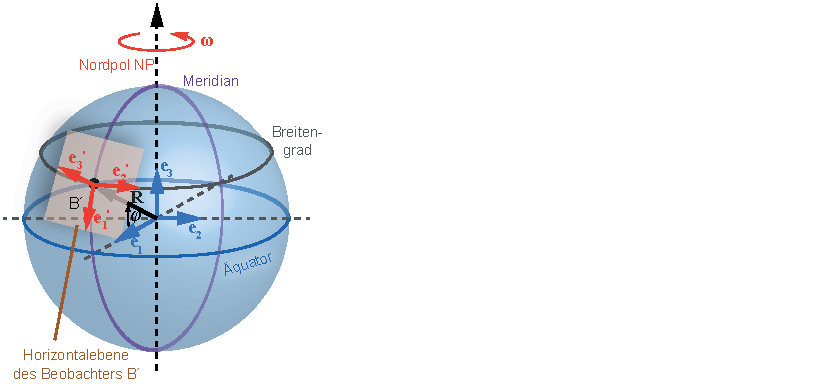
\includegraphics[scale=1]{Rot_Erde_1.pdf}
\caption[Inertialsystems und Nichtinertialsystem der rotierenden Erde.] {Darstellung des Inertialsystems $\vec{\Sigma} = (\veceX,\veceY,\veceZ) = (\vecez,\vecey,\vecez)$, in dem sich die Erde dreht. Das Nichtinertialsystem $\vec{\Sigma}' = (\vecpeX,\vecpeY,\vecpeZ)=(\vecpex,\vecpey,\vecpez)$ bewegt sich mit einem Beobachter B' auf der Erdoberfl�che mit.}\label{abb:bew_Rot_Erde1}
\end{figure}

\begin{figure}
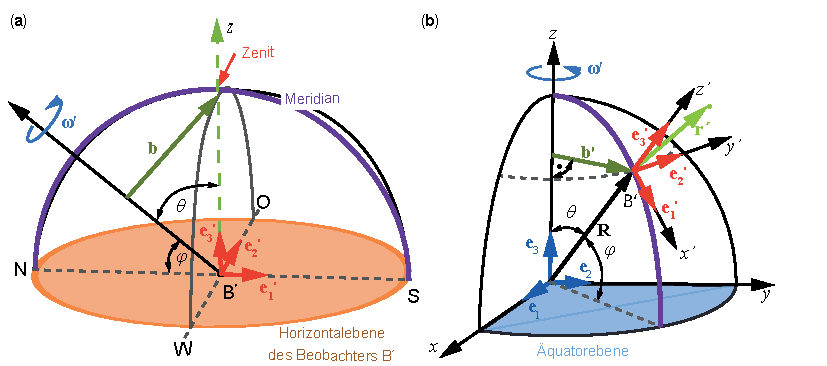
\includegraphics[scale=1]{Rot_Erde_4.pdf}
\caption[Bezugssysteme f�r die Behandlung der Erdrotation.]{Bezugssysteme f�r die Behandlung der Erdrotation. \fa Nichtinertialsystem, das sich mit einem Beobachter B' auf der Erdoberfl�che mitbewegt. Darstellung der beiden Bezugssysteme $\vec{\Sigma} = (\veceX,\veceY,\veceZ) = (\vecez,\vecey,\vecez)$ (Erde ruhend) und $\vec{\Sigma}' = (\vecpeX,\vecpeY,\vecpeZ)=(\vecpex,\vecpey,\vecpez)$. \fb Mitrotierender Beobachter auf der Erdoberfl�che.}\label{abb:bew_Rot_Erde4}
\end{figure}

Wir w�hlen das kartesische Inertialsystem $\vec{\Sigma}$ so, dass in dessen Ursprung der Mittelpunkt der rotierenden Erde liegt.
Das mitbewegte ebenfalls kartesische 
KOS $\vec{\Sigma} '$ sei mit einem beliebig w�hlbaren, aber festen Beobachterpunkt B' auf der Oberfl�che der Erde verbunden, der den Ursprung von $\vec{\Sigma} '$ bildet.
Somit rotiert das KOS $\vec{\Sigma} '$ zusammen mit dem Punkt B' relativ zu $\vec{\Sigma}$.
Die Erdrotation wird in $\vec{\Sigma}$ durch die Winkelgeschwindigkeit $\omega$ beschrieben, die f�r die Erde $2\pi/86164 \SI{}{\per\second} = \SI{7.292e-5}{\per\second}$ betr�gt.%
\footnote{Man beachte, dass man hier f�r die Erdumdrehung den siderischen Tag nehmen muss. In vielen Literaturstellen wird $\omega$ irrt�mlich mit $2\pi/86400 \SI{}{\per\second}$ angegeben, was der Dauer eines Sonnentages entspricht. Der Unterschied ist gering, aber nachweisbar, siehe auch Kapitel 3.1.2 in Himmelsmechanik (Band II, Kapitel 3).}
Wir w�hlen $\vec{\Sigma}'$ nun so, dass die $\vecpeZ$-Achse senkrecht von der Erdoberfl�che in den Himmel zeigt und die $\vecpeX$-Achse nach S�den.
Dann zeigt die $\vecpeY$-Achse nach Osten.

Bevor wir die verschiedenen Probleme und �bungen in Angriff nehmen, m�ssen wir etwas zum Vektor $\vec{\omega}'$ und zum Vektor $\vec{R}'$ erl�utern, da es hier immer wieder zu Problemen mit Vorzeichen und Zuordnung kommt.
Beide Vektoren m�ssen in den Basisvektoren von $\vec{\Sigma} '$, also den ${\vec{e}_i}'$, ausgedr�ckt werden.
Aus \figref{bew_Rot_Erde4} liest man ab:
\begin{align}
    \vec{\omega}' &= - \omega \cos{\varphi}\: \vecpeX + \omega \sin{\varphi}\: \vecpeZ\:=\: \omega\: \begin{pmatrix} -\cos{\varphi} \\ 0 \\ \sin{\varphi} \end{pmatrix} = \vec{\omega}'_{\|}  + \vec{\omega}'_{\bot} ~~~ \text{mit} \nonumber \\
    \vec{\omega}'_{\|} &= \begin{pmatrix} -\omega \cos{\varphi} \\ 0 \\ 0 \end{pmatrix} ~~\:\text{und}\:~~ \vec{\omega}'_{\bot}  = \begin{pmatrix} 0 \\ 0 \\ \omega \sin{\varphi} \end{pmatrix}~. \label{eq:bew_Omega_Ko}
\end{align} 
Der Winkel $\varphi$ wird dabei, wie in \figref{bew_Rot_Erde4} gezeigt, im System $\vec{\Sigma}$ gemessen.
F�r den Vektor $\vec{R}'$ gilt  $\vec{R}' = -R \:\vecpeZ$, da der Verschiebungsvektor im gestrichenen System vom Beobachter B' zum Erdmittelpunkt (Ursprung von $\vec\Sigma$) zeigt.
F�r die Erdoberfl�che gelten folgende Parameter:\\
\begin{align*}
	\dot{\vec{\omega}}' &= 0 ~,~~  \ddot{\vec{R}}' = 0 ~,~~  \dot{\vec{R}}' = 0 ~~,~ \vec{r} = \vec{R}'  + \vec{r}'\,,~\\ \text{und wegen } ~~\left|\vec{r}'\right| &\ll \min(\left|\vec{R}\right|, ~\left|\vec{r}\right|)~ \text{folgt}~~	\left|\vec{r}\right| \approx \left|\vec{R}\right|~.
\end{align*}
Wir starten von \eqref{eq:bew_Rot_System2} und erhalten mit   \eqref{eq:bew_Coriolis_Kraft} , \eqref{eq:bew_Zentrifugal_Kraft} und der Erdmasse $M_\text{E}$:
\begin{align}
	m\:\ddot{\vec{r}}'\;&= \;\vec{F_\text{G}} + \vec{F'_\text{Z}} + \vec{F'_\text{Cor}} \nonumber \\
	\Rightarrow \ddot{\vec{r}}'\;&= \;-\frac{G M_\text{E}}{r^3} \vec{r} - \underbrace{\vec{\omega}' \times \lk \vec{\omega}' \times  \vec{r}' \rk}_{\approx 0}  + \underbrace{\vec{\omega}' \times \lk \vec{\omega}' \times  \vec{R}' \rk}_{\vec{\omega}'(\vec{\omega}'\cdot\vec{R}') - \vec{R}'(\vec{\omega}'\cdot\vec{\omega}')}\: \: \underbrace{- 2 \vec{\omega}' \times \dot{\vec{r}}'}_{\vec{F}'_\text{Cor}/m} \nonumber \\
	\Rightarrow \ddot{\vec{r}}'\;&= \;- g_0 \:\vecpeZ \: + \: \underbrace{R \omega ^2 \lk\vecpeZ-\frac{\vec{\omega}'}{\omega ^2} (\vec{\omega}'\cdot \vecpeZ) \rk}_{\vec{b}'} \:- \:2 \vec{\omega}' \times \dot{\vec{r}}' \nonumber \\
	\Rightarrow \ddot{\vec{r}}'\;&= \;- \underbrace{\lk g_0 \:\vecpeZ \: - \: \vec{b}' \rk}_{\vec{g}'} \: \underbrace{-\: 2 \vec{\omega}' \times \dot{\vec{r}}'}_{\vec{F}'_\text{Cor}/m} ~.  \label{eq:bew_BGL_Erdrotation}
\end{align}
Mit \eqref{eq:bew_BGL_Erdrotation} haben wir die Bewegungsgleichungen f�r einen erdoberfl�chennahen K�rper im mitbewegten KOS auf der Erdoberfl�che gefunden.
Der Vektor $\vec{b}'$ ist ein Differenzvektor von $\vec{\omega}'$ und $\vecpeZ$ und ist auch in \figref{bew_Rot_Erde4} und \figref{bew_Rot_Erde5} eingezeichnet.
Er steht immer senkrecht auf $\vec{\omega}'$ und seine Komponenten k�nnen mit \eqref{eq:bew_Omega_Ko} zu 
\begin{align*}
    \vec{b}' &= R \omega^2 \lek \begin{pmatrix} 0 \\ 0 \\ 1 \end{pmatrix} - \begin{pmatrix} -\cos{\varphi}\cdot \sin{\varphi} \\ 0 \\ (\sin{\varphi})^2  \end{pmatrix}\rek \nonumber = R \omega^2 \lek \begin{pmatrix} + \frac{1}{2}\sin{2 \varphi} \\ 0 \\ 0  \end{pmatrix} + \begin{pmatrix} 0 \\ 0 \\ (\cos{\varphi})^2  \end{pmatrix} \rek \;=\;\:\vec{b}'_{\|} + \vec{b}'_{\bot} 
\end{align*}
berechnet werden.
Betrag und Richtung von $\vec{b}'$ sind damit abh�ngig von der geographischen Breite $\varphi$. 
Den Zusatzterm $\vec{b}'_{\bot}$ in radialer Richtung $\vecpeZ$ k�nnen wir mit der Schwerebeschleunigung $g_0 \cdot \vecpeZ$ zu einer effektiven Schwerebeschleunigung $\vec{g}_\text{eff}$ mit dem Betrag 
\begin{align}
	\vec{g}_\text{eff} \:=\: g_\text{eff} \,\vecpeZ \:= \:g_0 \,\vecpeZ - \vec{b}'_{\bot} \: =\: \lk \:g_0 -\: R \omega^2 (\cos{\varphi})^2\rk \vecpeZ\, \label{eq:bew_effektives_g}
\end{align} 
zusammenfassen.
Der tangentiale Zusatzterm $\vec{b}'_{\|}$ in S�d-Richtung $\vecpeX$ ist f�r $\varphi = 45\degree$ maximal und verschwindet an den Polen und am �quator.
Eine Folge dieser Kraftkomponente ist die Abplattung der Erde, denn die fr�her fl�ssige Erde stellte sich mit der Zeit so ein, dass die Oberfl�che senkrecht zur Resultierenden aus $\vec{g}_0$ und $\vec{b}'_{\|}$ liegt, also senkrecht zu $\vec{g}'$.\footnote{Man beachte, dass  $\vec{g}'$ nicht mehr zum Erdmittelpunkt zeigt (\probref{bew_AbplattungPlaneten}).}
Als Folge dieser Abplattung kommt es zu einer weiteren Abnahme der Schwerebeschleunigung am �quator �ber Gl. \eqref{eq:bew_effektives_g} hinaus, in welcher wir ja eine kugelf�rmige Erde angenommen hatten. Formel \eqref{eq:bew_effektives_g} bleibt dennoch eine gute N�herung.

\begin{figure}
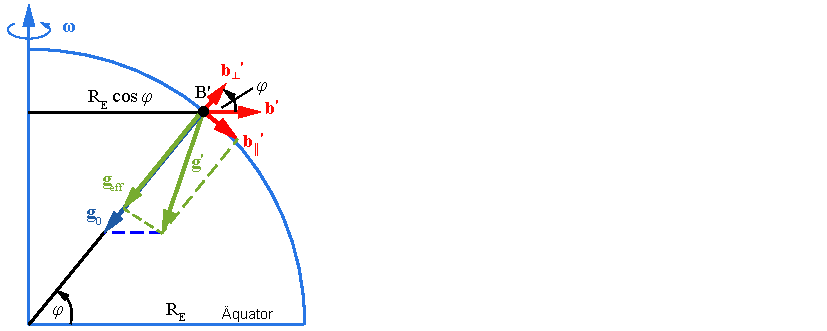
\includegraphics[scale=1]{Rot_Erde_5.pdf}
\caption[Abh�ngigkeit der Schwerebeschleunigung von der geographischen Breite.] {Abh�ngigkeit der Schwerebeschleunigung von der geographischen Breite $\varphi$. Zur Deutlichkeit sind die L�ngenverh�ltnisse stark �bertrieben. Man mache sich klar, dass $\left| \vec{b}' \right| \approx 0.05 \,g$ ist. Ebenso m�ge der Leser das Bild f�r die s�dliche Hemisph�re zeichnen, um zu erkennen, dass wegen der $\sin{\varphi}$-Abh�ngigkeit die Komponente $\vec{b}'_{\|}$ nach Norden zeigt.}
\label{abb:bew_Rot_Erde5}
\end{figure}

Wir wenden uns jetzt dem Term der Coriolis-Kraft $\vec{F'_\text{Cor}}$ zu.
Wegen \eqref{eq:bew_Omega_Ko} und $\dot{\vec{R}}'= 0 $ kann diese in zwei Komponenten zerlegt werden:
\begin{align}
	\vec{F'_\text{Cor}} = - 2 m \lek \lk \vec{\omega}'_{\bot}  \times \dot{\vec{r}}' \rk + \lk \vec{\omega}'_{\|} \times  \dot{\vec{r}}' \rk \rek ~. \label{eq:bew_Coriolis_Ko}
\end{align} 
Der Term mit $\vec{\omega}'_{\bot}$ f�hrt bei einer Bewegung auf der Erdoberfl�che zu einer seitlichen Ablenkung, w�hrend der Term mit $\vec{\omega}'_{\|}$ zu einer vertikal (aufw�rts oder abw�rts) gerichteten Kraft f�hrt.
Die seitlich gerichtete Kraft ist von gro�er Bedeutung f�r Zyklone, Meeresstr�mungen und die Ballistik (\probref{bew_Coriolis_I}--\probref{bew_Coriolis_III}).
Um die Effekte, die durch die Coriolis-Kraft im mitbewegten System auftreten, besser berechnen und verstehen zu k�nnen, schreiben wir \eqref{eq:bew_BGL_Erdrotation} in den einzelnen Komponenten:
\begin{align}
    \begin{pmatrix} \ddot{x}' \\  \ddot{y}' \\  \ddot{z}' \end{pmatrix} \:=\: - 2 \omega \: \begin{pmatrix} -\frac{1}{4} R \omega \sin{2\varphi} - \dot{y}' \sin{\varphi} \\ \dot{x}' \sin{\varphi} + \dot{z}' \cos{\varphi} \\ -\dot{y}' \cos{\varphi} + g_\text{eff}/(2 \omega) \end{pmatrix} ~. \label{eq:bew_BGL_Erdrotation_Ko}
\end{align}
Wir haben mit \eqref{eq:bew_BGL_Erdrotation_Ko} ein System dreier gekoppelter Differentialgleichungen als Bewegungsgleichungen f�r Massepunkte im mitbewegten System gewonnen.
Diese Gleichungen k�nnen numerisch f�r verschiedene Anfangsbedingungen gel�st werden (\probref{bew_Coriolis_I}).
Um eine N�herungsl�sung f�r $\omega \,t \ll 1$ (was bei den betrachteten Bewegungen nahe der Erdoberfl�che erf�llt ist) angeben zu k�nnen, mit der man die wesentlichen Effekte erkennen kann, vernachl�ssigen wir alle Terme mit $\omega^2$.
Einmalige Integration von \eqref{eq:bew_BGL_Erdrotation_Ko} ergibt:
\begin{align}
    \begin{pmatrix} \dot{x}' \\  \dot{y}' \\  \dot{z}' \end{pmatrix}\:=\: \: \begin{pmatrix} 2 \omega y' \sin{\varphi} + C_x\\ - 2 \omega\ \lk x' \sin{\varphi} + z' \cos{\varphi} \rk + C_y \\ 2 \omega y' \cos{\varphi} - g_\text{eff}\,t + C_z \end{pmatrix}~. \label{eq:bew_BGL_Erdrotation_Approx1}
\end{align}
F�r den \emph{freien Fall} \index{Fall!freier} ergeben sich aus den Anfangsbedingungen
	\[x'(0) =\: y'(0) =\: \dot{x}'(0) =\: \dot{y}'(0) =\: \dot{z}'(0) =\: 0 \quad \text{und} \quad z'(0) =\: h 
\]
die Integrationskonstanten zu $C_x = C_z = 0$ und $C_y = 2 \omega h \cos{\varphi}$. 
In \eqref{eq:bew_BGL_Erdrotation_Approx1} kann man wiederum alle Terme mit $ \omega x'$ und $\omega y'$ vernachl�ssigen, da $x'$ und $y'$ selbst proportional zu $\omega$ sind, woraus n�herungsweise
\begin{align}
    \begin{pmatrix} \dot{x}' \\  \dot{y}' \\  \dot{z}' \end{pmatrix}\: \approx \: \begin{pmatrix} 0 \\ 2 \omega \lk h -  z' \rk \cos{\varphi} \\ - g_\text{eff}\,t \end{pmatrix} \label{eq:bew_BGL_Erdrotation_Approx2}
\end{align}
folgt. 
Mit $g_\text{eff} \approx g$ folgt f�r die $z'$-Komponente die bekannte L�sung f�r den freien Fall und f�r die beiden anderen Komponenten durch Einsetzen der L�sung f�r $z'(t)$ und unter Ber�cksichtigung der Anfangsbedingungen schlie�lich als N�herungsl�sung
\begin{align}
    \begin{pmatrix} x'(t) \\ y'(t) \\ z'(t) \end{pmatrix}\:=\: \: \begin{pmatrix} 0 \\ \omega\ g \frac{t^3}{3} \cos{\varphi} \\ h - g \frac{t^2}{2} \end{pmatrix}~. \label{eq:bew_BGL_Erdrotation_Lsg1}
\end{align}
F�r eine Fallzeit $t_f = \sqrt{\frac{2h}{g}}$ (aus $z'(t_f) = 0$) ergibt sich f�r die interessante $y'$-Komponente 
\begin{align}
	y'_f = \frac{2 \omega h \cos{\varphi}}{3} \sqrt{\frac{2h}{g}} ~.\label{eq:bew_BGL_Erdrotation_Lsg2}
\end{align}
F�r einen frei fallenden K�rper kommt es also zu einer Ostablenkung, die am �quator am gr��ten ist.
Man kann sich leicht �berlegen, dass die Coriolis-Kraft auf andere ballistische und Bewegungsph�nomene auf der Erde einen nicht zu vernachl�ssigenden Einfluss hat.
Gleichungssystem \eqref{eq:bew_BGL_Erdrotation_Ko} gibt uns die Grundlage daf�r, einige dieser Effekte,
die ein Beobachter auf der Erdoberfl�che \anf{sieht},
wie \zb Projektilabweichungen und Zyklonrichtungen\index{Zyklon}%
\footnote{Ein Zyklon ist ein tropischer Wirbelsturm im indischen und s�dlichen pazifischen Ozean.
Dagegen werden mit Hurrikans Wirbelst�rme bezeichnet, die an den K�sten des amerikanischen Doppelkontinents auftreten.
Wirbelst�rme in Ost- und S�dostasien hingegen werden Taifune genannt.
Wir benutzen Zyklone als �berbegriff.} erkl�ren und berechnen zu k�nnen (\probref{bew_Coriolis_III}).

\subsection{Oszillatoren und Pendel}\index{Pendel} \label{kap:bew_pendulum}

Wir hatten uns bereits in \kap{bew_schwingung} auf der Basis des Lagrange-Formalismus mit den grundlegenden Bewegungsgleichungen f�r schwingende Systeme besch�ftigt.
Wie dort erl�utert, findet man solche Systeme an vielen Stellen in der Natur und damit auch in der Physik.
Wir wollen das Thema deswegen in diesem Kapitel mit einigen konkreten Beispielen vertiefen.  
Wir werden dabei die Vielfalt der schwingenden Systeme kennenlernen und uns dar�ber hinaus auch mit den Ph�nomenen der Reibung, der Resonanz und der nichtlinearen Kopplung besch�ftigen.
Letztere liefern uns eine Reihe von \zt �berraschenden Effekten bis hin zu chaotischem Verhalten.
Es ist auch erstaunlich, wie viele ber�hmte Physiker sich �ber die Jahrhunderte hinweg mit der Theorie schwingender Systeme, insbesondere mit Pendelproblemen, besch�ftigt haben.
Das Pendel hat �ber lange Zeit hinweg eine wesentliche Rolle bei der Zeitmessung gespielt. 
Auch Philosophen und K�nstler wurden vielfach von den Schwingungen des Pendels inspiriert.
Wir empfehlen dem interessierten Leser, in der sehr sch�nen und umfangreichen Zusammenfassung zur Physik, Geschichte und Kunst rund um das Pendel in \cite{Matthews2005} zu lesen.

\subsubsection{Der harmonische Oszillator} \index{Oszillator!harmonischer|textbf} \label{kap:bew_harmon_oszillator}

Wir beginnen mit dem harmonischen Oszillator, dessen Bewegungsgleichung wir bereits in \kap{bew_schwingung} als Grenzfall f�r kleine Schwingungen hergeleitet hatten, siehe Gleichung \eqref{eq:bew_Schwingung01a}. 
Die Lagrange-Funktion\index{Lagrange-Funktio} des eindimensionalen harmonischen Oszillators hatten wir bereits in den Kapiteln \ref{kap:bew_Lagrange_II} und \ref{kap:bew_Lagrange_II_R} aufgestellt:
\begin{align}
	\mathcal{L} = \frac{1}{2} m \,\dot{q}^2 \,-\,\frac{1}{2} k\,q^2 \,. \label{eq:bew_pendulum01}
\end{align}
Wir k�nnen daraus die Bewegungsgleichung f�r die verallgemeinerte Koordinate $q$ ableiten, indem wir die Lagrange-Funktion um einen Reibungsterm und eine zeitlich variierende externe Kraft erweitern. 
Wir erhalten
\begin{align}
	\ddot{q} + \eta_n \,\dot{q}^n + {\omega_0}^2 \, q \,=\, \frac{F^{\text{\,(ext)}}(t)}{m} = \frac{F_\text{A}\,\cos(\omega_\text{A}t + \delta_\text{A})}{m}\label{eq:bew_pendulum02}
\end{align}
mit ${\omega_0}^2 = k/m$ und einem Reibungskoeffizienten $\eta_n$, wobei $n$ entweder $1$ oder $2$ ist.
Hierbei haben wir eine (verallgemeinerte) externe Kraft $F^{\text{ext}}(t)$ als harmonische Schwingung mit einer Anregungsfrequenz $\omega_\text{A}$ und einer Amplitude von $F_\text{A}$ angenommen.
Wir behandeln den Fall $n=1$.
Dann ist \eqref{eq:bew_pendulum02} eine lineare inhomogene Differentialgleichung (DGL), in der wir, um etwas Schreibarbeit zu sparen, $\eta_1 = 2 \gamma$ setzen.
Dann erhalten wir mit dem gleichen Ansatz $Q = Q_0 \mathrm{e}^{\mathrm{i}\omega t}$ wie in \eqref{eq:bew_Schwingung03} f�r die homogene DGL die Bestimmungsgleichung
\begin{align*}
	\lk -\omega^2 + 2\gamma \, \mathrm{i} \,\omega + {\omega_0}^2 \rk \, \mathrm{e}^{\mathrm{i} \omega t} = 0\,,
\end{align*}
woraus sich die Schwingungsfrequenz wie folgt ergibt:
\begin{align}
	\omega = \mathrm{i} \, \gamma \pm \sqrt{{\omega_0}^2 - \gamma^2} = \mathrm{i} \, \gamma \pm \hat{\omega}~. \label{eq:bew_pendulum03}
\end{align}
Je nach Verh�ltnis von $\omega_0$ und $\gamma$ k�nnen wir die folgenden drei F�lle unterscheiden:
\begin{enumerate} [a) ]
	\item \textit{Schwache D�mpfung, bei} $\omega_0 > \gamma$\\
	Die allgemeine L�sung ist mit einem rellen $\hat{\omega}$ gegeben durch
	\begin{align}
		q(t) = A \mathrm{e}^{-\gamma t}  \sin(\hat{\omega}\,t + \phi) \,, \label{eq:bew_pendulum04}
	\end{align}
	worin $A$ und $\phi$ durch die Anfangsbedingungen gegeben sind.
        Man erkennt, dass die Frequenz $\omega$ des schwach ged�mpften Oszillators leicht zu niedrigeren Frequenzen gegen�ber der Eigenfrequenz $\omega_0$ verschoben ist.
	\item \textit{Starke D�mpfung, bei} $\omega_0 < \gamma$\\
	Hier ist die allgemeine L�sung mit einem rein imagin�ren $\hat{\omega}$, gegeben durch
	\begin{align}
		q(t) = A \mathrm{e}^{-\gamma_1 t} + B \mathrm{e}^{-\gamma_2 t} \,, \label{eq:bew_pendulum05}
	\end{align}
	mit
		\[\gamma_{1,2} = \gamma \pm \sqrt{\gamma^2 - {\omega_0}^2} = \gamma \pm \mathrm{i}\, \hat{\omega} \,.
	\]
	$A$ und $B$ werden wieder durch die Anfangsbedingungen bestimmt.
        Man erkennt, dass es beim stark ged�mpften Oszillator keine Schwingungen gibt.
	\item \textit{Kritische D�mpfung -- aperiodischer Grenzfall, bei} $\omega_0 = \gamma$\\
	Hier ist die allgemeine L�sung durch
	\begin{align}
		q(t) = \lk A + B\, t \rk \mathrm{e}^{-\gamma t} \label{eq:bew_pendulum06}
	\end{align}
gegeben.\footnote{Man beachte, dass man nicht einfach in \eqref{eq:bew_pendulum04} $\gamma_1=\gamma_2$ setzen kann, da wir wegen der DGL zweiter Ordnung zwei linear unabh�ngige L�sungen brauchen.
Siehe dazu auch \cite{Riley2006} und \cite{Otto2019, Fischer2018}.
Man kann aber L�sung \eqref{eq:bew_pendulum06} �ber eine Grenzfallbetrachtung aus \eqref{eq:bew_pendulum04} herleiten.}
Man erkennt aus \figref{bew_HarmonOszillator01}, dass der aperiodische Grenzfall die schnell\-ste D�mpfung des schwingenden Systems ergibt.
$A$ und $B$ werden wieder durch die Anfangsbedingungen bestimmt. 
\end{enumerate}
Um die DGL f�r eine erzwungene Schwingung zu l�sen, muss man eine spezielle L�sung der inhomogenen DGL zur allgemeinen L�sung der homogenen DGL addieren.
Auch dazu machen wir wieder den Ansatz $Q_\text{p} = Q_\text{p0} \, \mathrm{e}^{\mathrm{i}\omega t}$ und erhalten als Bestimmungsgleichung
\begin{align}
	 Q_\text{p0} = \frac{F_\text{A}}{m} \frac{1}{{\omega_0}^2-{\omega_\text{A}}^2 + 2\,\mathrm{i} \,\gamma \omega_\text{A}}\,.\label{eq:bew_pendulum07}  
\end{align}

Da im Allgemeinen $\gamma \neq 0$ gilt, ist $Q_\text{p0}$ eine komplexe Zahl, die wir als
\begin{align*}
	Q_\text{p0} = \Re \, Q_\text{p0} + \im\,\Im \, Q_\text{p0}
\end{align*}
darstellen k�nnen mit
\begin{align}
 	\Re \, Q_\text{p0} &= \frac{F_\text{A}}{m} \frac{({\omega_0}^2 - {\omega_\text{A}}^2)}{( {\omega_0}^2 - {\omega_\text{A}}^2)^2 + 4 \gamma^2 \,{\omega_\text{A}}^2 }\,,
 	\label{eq:bew_pendulum08} \\
 	\Im \, Q_\text{p0} &= - \frac{F_\text{A}}{m} \frac{2 \omega_\text{A}\, \gamma}{( {\omega_0}^2 - {\omega_\text{A}}^2)^2 + 4 \gamma^2 \,{\omega_\text{A}}^2 } \,. \label{eq:bew_pendulum09}
 \end{align} 
Wir k�nnen daraus die allgemeine L�sung der inhomogenen DGL f�r $q(t)$ herleiten:
\begin{align}
	q(t) = A(\omega_\text{A}) \cos(\omega_\text{A}t - \varphi(\omega_\text{A})) 
		+ \hat{A} \mathrm{e}^{- \gamma t} \cos \lk \hat{\omega}t - \hat{\delta}\rk
		\label{eq:bew_pendulum10}
\end{align}
mit
\begin{align*}
	A(\omega_\text{A}) &= \frac{F_\text{A}}{m} \frac{1}{\sqrt{({\omega_0}^2 - {\omega_\text{A}}^2)^2 + 4 \gamma^2 \, {\omega_\text{A}}^2}} \\
	\varphi(\omega_\text{A}) &= - \frac{\Im \, Q_\text{p0}}{\Re \, Q_\text{p0}} 
	= \arctan \lk \frac{2 \gamma \,\omega_0}{{\omega_0}^2 - {\omega_\text{A}}^2} \rk \\
 \hat{\omega} &= \sqrt{{\omega_0}^2 - \gamma^2} \,. 
\end{align*}
Die Parameter $\hat{A}$ und $\hat{\delta}$ bestimmen sich wieder aus den Anfangsbedingungen.
Man erkennt folgendes:
\begin{itemize}
	\item F�r $t \gg 1/\gamma$ bleibt nur die spezielle L�sung �brig, \dh nach dem Einschwingen schwingt der Oszillator mit der Frequenz $\omega_\text{A}$.
	\item W�hrend des Einschwingens kann es zu Schwebungen zwischen $\omega_0$ und $\omega_\text{A}$ kommen.
          Diese dauern umso l�nger, je geringer die D�mpfung ist.
	\item Amplitude $A(\omega_\text{A})$ und Phasenlage $\varphi(\omega_\text{A})$ h�ngen von der Anregungsfrequenz $\omega_\text{A}$ ab. 
	Die Resonanzfrequenz der Amplitude ist gegeben durch
	\[\omega_\text{max} = \sqrt{{\omega_0}^2 - 2\gamma^2}~\] und ergibt eine maximale Amplitude von 	
		\[A_\text{max}(\omega_\text{max}) = \frac{F_\text{A}}{m}\frac{1}{2\gamma \sqrt{{\omega_0}^2-\gamma^2}}\,.
	\]
	\item Die Halbwertsbreite der Resonanz ist durch
	\[ \delta_\omega = \omega_+ - \omega_-  
	\qquad \text{mit} \qquad 
	{\omega_\pm}^2 = {\omega_0}^2 - 2 \gamma^2 \pm 2 \gamma \sqrt{{\omega_0}^2 - \gamma^2}\]
	gegeben.
	Man erkennt, dass die Halbwertsbreite gr��er ist, je gr��er die D�mpfung ist.\footnote{Die Halbwertsbreite wird �ber die Gr��e $(A(\omega_\text{A}))^2$ bestimmt, da man \ia als Messgr��e die Intensit�t verwendet, welche proportional zum Quadrat der Amplitude $A$ ist.}
	\item F�r $\gamma \ll \omega_0$ gehen die Beziehungen �ber in
		\begin{align*}
			A_\text{max} &= \frac{F_\text{A}}{m} \frac{1}{2 \gamma\, \omega_0} \,,\\
			\omega_\text{max} &= \omega_0 - \frac{\gamma^2}{\omega_0} \approx \omega_0 \,,\\
			\delta_\omega &= 2 \gamma \,.
		\end{align*}
\end{itemize}
Wir m�chten an dieser Stelle darauf hinweisen, dass wir bei unseren Rechnungen immer noch kleine Auslenkungen $q$ angenommen haben.
Das mag aber insbesondere im Resonanzfall nicht immer erf�llt sein, weswegen man dann zur exakten L�sung �bergehen muss.
Diese werden wir im n�chsten Kapitel behandeln.

Zuvor wollen wir noch die Leistungs�bertragung von der Anregungsquelle auf den Oszillator betrachten.
Da das System nicht konservativ ist, gibt es eine Verlustleistung der Anregungsquelle.
Diese ist gegeben durch
\[  P_\text{V} = - \eta_1 \,m \,\dot{q}\,\dot{q} = -2 \gamma\,m \,\dot{q}^2 \]
\bzw zeitlich gemittelt
\begin{align}
	\left\langle P_\text{V} \right\rangle  &= \frac{1}{T} \int_0^T P_\text{V}(t') \, \D t' = -2 \gamma m \lek A(\omega_\text{A})\rek^2 {\omega_\text{A}}^2 \left\langle \sin^2(\omega_\text{A}t - \delta_\text{A}) \right\rangle \nonumber \\
	&= - \gamma m \lek A(\omega_\text{A})\rek^2  {\omega_\text{A}}^2 \, , \label{eq:bew_pendulum12}
\end{align}
weil \[ \bigintssss_0^{T=\frac{2 \pi}{\omega_\text{A}}} \sin^2(\omega_\text{A}t' - \delta_\text{A}) \, \mathrm{d}t' = \frac{1}{2}\] ist. 
Man erkennt auch, dass die Verlustleistung bei Resonanz am gr��ten ist, \dh dass in diesem Fall die meiste Energie von der Quelle auf den Oszillator �bergeht.  

Im \mscr{} \mlbewref{HarmonOszillator.m} sind die Rechnungen im Detail ausgef�hrt und einige Diagramme daraus bereits in \figref{bew_HarmonOszillator01} und \figref{bew_HarmonOszillator02} gezeigt.
Wir weisen darauf hin, dass $\eta_1$ bzw. $\gamma$ dieselbe Einheit besitzen wie $\omega_0$, also $\si{s^{-1}}$.
Darum kann $1/\gamma$ als die Zeitspanne interpretiert werden, nach der die Oszillation stark abgeklungen ist.
In \probRef{bew_HO_quadrat} wird auch der Fall f�r eine quadratisch von der Geschwindigkeit abh�ngende Reibung numerisch behandelt.
Reibungskr�fte, die quadratisch in $\dot{q}$ sind, machen die mathematische Behandlung wesentlich komplizierter, da die Bewegungsgleichung dann nichtlinear ist.
Wir geben in der L�sung zu \probref{bew_HO_quadrat} auch die weiterf�hrende Literatur \cite{Smith2012} zur analytischen Behandlung dieser nichtlinearen DGL an und vergleichen die analytische mit unserer numerischen L�sung.

\begin{figure}
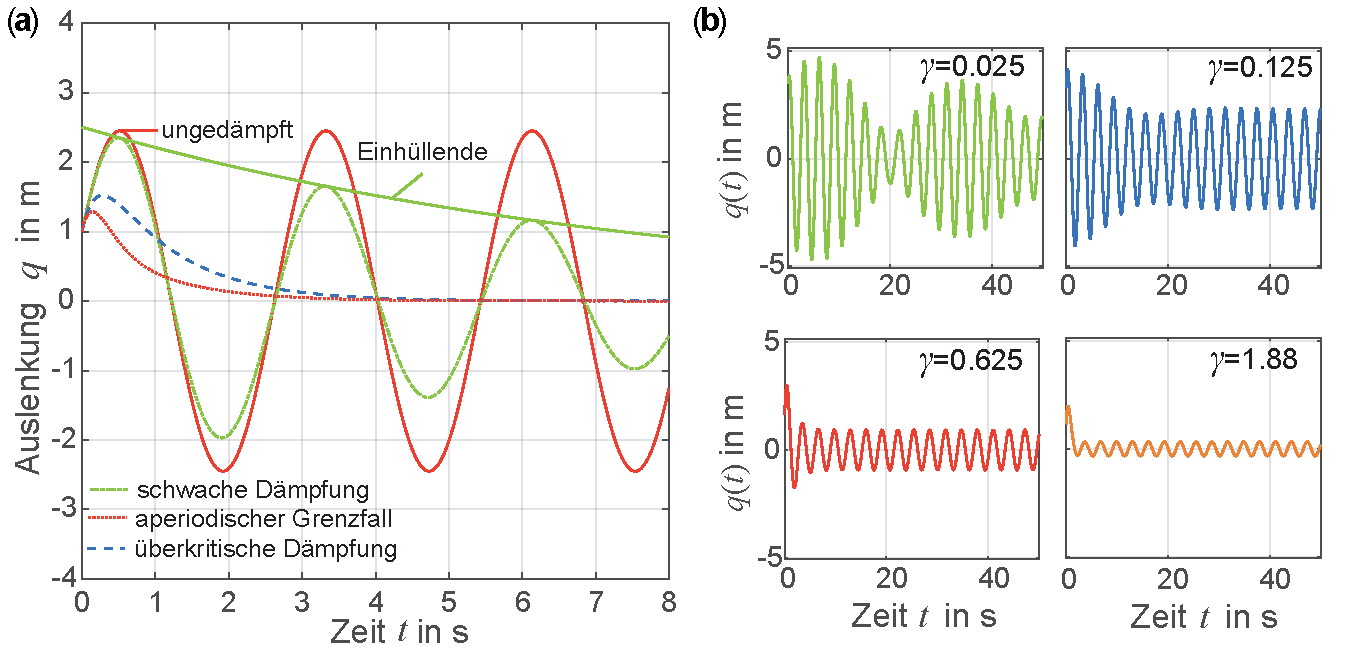
\includegraphics[width=\textwidth]{HarmonOszillator01.pdf}
\caption[D�mpfung des harmonischen Oszillators und Einschwingverhalten.] {\fa D�mpfung des harmonischen Oszillators und \fb dessen Einschwingverhalten f�r verschiedene Reibungskoeffizienten $\gamma$ und $\omega_0/\omega_\text{A}=0.9$.} 
\label{abb:bew_HarmonOszillator01}
\end{figure}

\begin{figure}
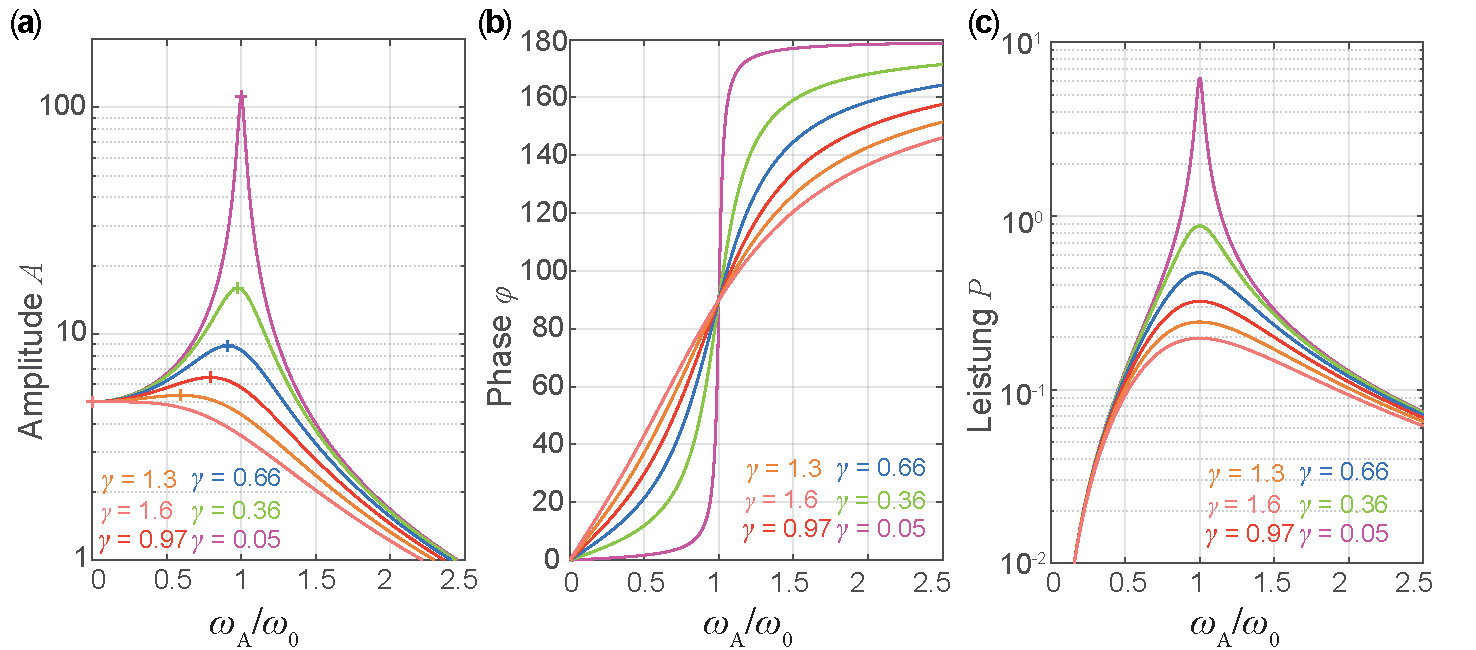
\includegraphics[width=\textwidth]{HarmonOszillator02.pdf}
\caption[Amplitude, Phase und Leistungs�bertragung eines Oszillators.] {\fa Amplitude, \fb Phasen und \fc Leistungs�bertragung beim getriebenen harmonischen Oszillator f�r verschiedene Anregungsfrequenzen und Reibungen.} 
\label{abb:bew_HarmonOszillator02}
\end{figure}

\subsubsection{Der anharmonische Oszillator (Nichtlineares Pendel)} \index{Oszillator!harmonischer} \index{Oszillator!anharmonischer} \index{Pendel!nichtlineares}\index{Pendel!mathematisches}\label{kap:bew_anharmon_oszillator}

Wir haben uns im vorherigen Kapitel auf kleine Schwingungen beschr�nkt, f�r die die Linearisierung \bzw die sogenannte harmonische N�herung galt. 
Wir wollen diese Beschr�nkung jetzt aufgeben und sowohl eine analytische L�sung als auch gut handhabbare N�herungsl�sungen f�r dieses allgemeinere Problem finden. 
Dazu machen wir uns zun�chst noch einmal klar, dass in der linearen N�herung \eqref{eq:bew_pendulum01} die potentielle Energie in der Lagrange-Funktion �berbewertet wird und daher zu erwarten ist, dass in der exakten L�sung des Oszillators die Schwingungsperiode (Eigenfrequenz) von der Amplitude abh�ngig sein wird, und zwar so, dass mit steigender Amplitude auch die Schwingungsperiode zunimmt.
Das erkennt man auch leicht, wenn man in \eqref{eq:bew_Schwingung_d} \bzw \eqref{eq:bew_Schwingung01b} noch den n�chsten Term der Sinus-Entwicklung mitnimmt, der dann wie eine Verringerung der Schwingungskreisfrequenz wirkt.
Die Bewegungsgleichung lautet dann
\begin{align}
                \ddot{\theta}+{\omega_0}^2\, \theta = \frac{{\omega_0}^2\,\theta^3}{6} \ =\kappa_3\,\theta^3 \,. \label{eq:bew_NLOsz01}
\end{align}
F�r einen beliebigen anharmonischen Oszillator gilt ganz allgemein
\begin{align}
                \ddot{x}+{\omega_0}^2 x= \kappa_2\, x^2+\kappa_3 \,x^3 + \ldots = \sum\limits_{j} \kappa_j\,x^j \,.   \label{eq:bew_NLOsz02}
\end{align}

\subparagraph{\textbf{Ansatzmethode zur Berechnung der Schwingungsperiode des nichtlinearen Pendels}}

Wir wollen in unserer Betrachtung auch den Fall einer m�glichen asymmetrischen Schwingung ber�cksichtigen und machen daher den allgemeinen Ansatz
	\begin{align}
			x(t) = A_0 + A_1\cos\omega t + A_2\cos2\omega t + A_3\cos3\omega t \,. \label{eq:bew_NLOsz03}
	\end{align}
Wir setzen diesen Ansatz nun in \eqref{eq:bew_NLOsz02} ein und erhalten f�r die Ableitung auf der linken Seite von \eqref{eq:bew_NLOsz02}
\begin{align}
\ddot{x}  =  - \omega^2 A_1\cos\omega t - 4 \omega^2 A_2\cos2\omega t - 9 \omega^2 A_3\cos3\omega t~. \label{eq:bew_NLOsz03a}
\end{align}
Auf der rechten Seite von \eqref{eq:bew_NLOsz02} ergeben sich dann Terme aus den Potenzen in $x$, bei deren Berechnung wir von verschiedenen trigonometrischen Formeln f�r die Potenzen der Winkelfunkionen Gebrauch machen, insbesondere von  $\cos^2 (\omega t) = (1+ \cos \lk 2 \omega t \rk)/2$ und $\cos^3(\omega t) = (3 \cos \omega t + \cos \lk 3 \omega t \rk)/4$. Wir wollen auch nur die Terme mit Potenzen bis ${A_3}^3$ und Frequenzen bis $3\omega t$ mitnehmen, da wir annehmen wollen, dass $A_2, A_3 \ll A_1$. Es ergeben sich dann folgende Terme:
\begin{align} 
\begin{split}
 \text{f�r}~ x^1 &: A_0 + A_1\cos\omega t + A_2\cos2\omega t + A_3\cos3\omega t \,, \\
 \text{f�r}~ x^2 &: {A_0}^2 + \frac{1}{2} {A_1}^2\cos2\omega t + \frac{1}{2} \lk {A_1}^2 + {A_2}^2 + {A_3}^2 \rk\,, \\
 \text{f�r}~ x^3 &: {A_0}^3 + \frac{3}{4} {A_1}^3\cos\omega t + \frac{3}{4} {A_2}^3\cos2\omega t + \frac{1}{4} \lk {A_1}^3 + 3{A_3}^3 \rk \cos3\omega t \,.
\label{eq:bew_NLOsz04} 
\end{split} 
\end{align}
Wir bringen nun \eqref{eq:bew_NLOsz03a} und \eqref{eq:bew_NLOsz04} zusammen in die Form  
\begin{align}
	T_0 + T_1 A_1 \cos\omega t + T_2 A_2 \cos2\omega t + T_3 A_3 \cos3\omega t = 0   \label{eq:bew_NLOsz05a}
\end{align}
und sortieren nach Argumenten der Winkelfunktionen in die einzelnen Terme $T_i$:
\begin{align} \begin{split}
 \text{f�r}~ \cos 0\omega t &: \qquad  T_0 = A_0 {\omega_0}^2 -\kappa_2 \lk {A_0}^2 + \lk {A_1}^2+{A_2}^2+{A_3}^2 \rk \rk - \kappa_3 {A_0}^3 \,, \\
 \text{f�r}~ \cos 1\omega t &: \qquad  T_1 = - \omega^2 + {\omega_0}^2 - 3 \kappa_3 \frac{{A_1}^2}{4}\,, \\
 \text{f�r}~ \cos 2\omega t &: \qquad  T_2 = A_2 {\omega_0}^2 - 4 A_2 \omega^2 - \kappa_2 \frac{{A_1}^2}{2} - 3 \kappa_3 \frac{{A_2}^3}{4}\,, \\
 \text{f�r}~ \cos 3\omega t &: \qquad  T_3 = A_3 {\omega_0}^2 - 9 A_3 \omega^2 - \frac{\kappa_3}{4} \lk {A_1}^3 + 3 {A_3}^3 \rk \,. \label{eq:bew_NLOsz05} 
\end{split} \end{align}
Damit Bestimmungsgleichung \eqref{eq:bew_NLOsz05a} erf�llt werden kann,
m�ssen alle Terme $T_i$ einzeln verschwinden,
da \eqref{eq:bew_NLOsz05a} f�r alle Zeiten Null sein muss.
Aus $T_1$ in \eqref{eq:bew_NLOsz05} folgt dann sofort $\omega^2 = {\omega_0}^2 - \frac{3\kappa_3}{4} {A_1}^2$ und damit
\begin{equation}
    \omega = \omega_0 \sqrt{1 - \frac{3\,\kappa_3}{\lk 2 \omega_0 \rk^2} {A_1}^2}
    \label{eq:bew_NLOsz06}~,
\end{equation}
was bedeutet, dass die Kreisfrequenz des anharmonischen Oszillators wie erwartet kleiner ist als die des harmonischen Oszillators
und dar�ber hinaus von der Amplitude $A_1$ abh�ngt.
Aus der Bedingung $T_3=0$ folgt dann f�r ${A_3}^3 \approx 0$ (wegen $A_3 \ll A_1$) die Beziehung
\begin{equation}
    A_3 \approx \frac{\kappa_3 {A_1}^3}{27\,\kappa\, {A_1}^2 - 32\, {\omega_0}^2} \label{eq:bew_NLOsz07}~.
\end{equation}
Gehen wir nun speziell zum Fall des \textit{nichtlinearen Pendels} �ber, dann folgt mit $\kappa_2 = 0$ aus den Termen $T_0\,, T_2$ sofort $A_0 =0\,, A_2=0$ und wir k�nnen unsere L�sung aufschreiben als
\begin{equation}
    \theta(t) = \theta_A \, \cos(\omega\,t) + {\theta_A}^3 \lk \frac{1}{27\,{\theta_A}^2-192} \rk \, \cos(3\, \omega\,t) \label{eq:bew_NLOsz08}
\end{equation}
mit der Schwingungsfrequenz \bzw der Schwingungsperiode 
\begin{align} 
\begin{split}
			\omega &= \omega_0 ~ \sqrt{1-\frac{{\theta_\text{A}}^2}{8}}\,,~~T_\text{P} = \frac{T_0}{\sqrt{1-{\theta_\text{A}}^2/8}} \,. \label{eq:bew_NLOsz12}
\end{split}
\end{align}
Wie erwartet wird die Schwingungsperiode mit zunehmender Auslenkung gr��er. In der Literatur \cite{Hinrichsen2021} findet man eine ganze Reihe �hnlicher N�herungen f�r die Schwingungsperiode \eqref{eq:bew_NLOsz12}, die im Allgemeinen auf der Basis verschiedener N�herungen in der Taylor-Entwicklung beruhen. Jakob Bernoulli\indexp{Bernoulli, Jakob}\footnote{Jakob Bernoulli (1655--1705) war ein Schweizer Mathematiker und Physiker, der wesentlich zur Entwicklung der Wahrscheinlichkeitstheorie sowie zur Variationsrechnung und zur Untersuchung von Potenzreihen beigetragen hat.} gab bereits 1749 eine sehr gute N�herung mit 
\begin{equation}
    T_B(\theta_\text{A}) = T_0 \lk 1 + \frac{{\theta_\text{A}}^2}{16}\rk \label{eq:bew_NLOsz09}
\end{equation}
an.
Weitere interessante N�herungen sind 
  \begin{align}
    T_{\text{KF}} = T_0 \frac{1}{\sqrt{\cos \lk \frac{\theta_\text{A}}{2}\rk}} ~~\text{\cite{Hinrichsen2021,Kidd2002} ~~und} ~~
    T_{\text{DE}} = T_0 \frac{1}{1- \frac{{\theta_\text{A}}^2}{16}} ~~\text{\cite{Denman1959}} \,.
  \end{align}
\figref{bew_NLOsz01} vergleicht diese verschiedenen N�herungen (\mscr{} \mlbewref{AnHarmonOszillator01.m}) mit der exakten analytischen Berechnung der Schwingungsperiode �ber das elliptische Integral, die wir im Folgenden vornehmen wollen. 

\begin{figure}
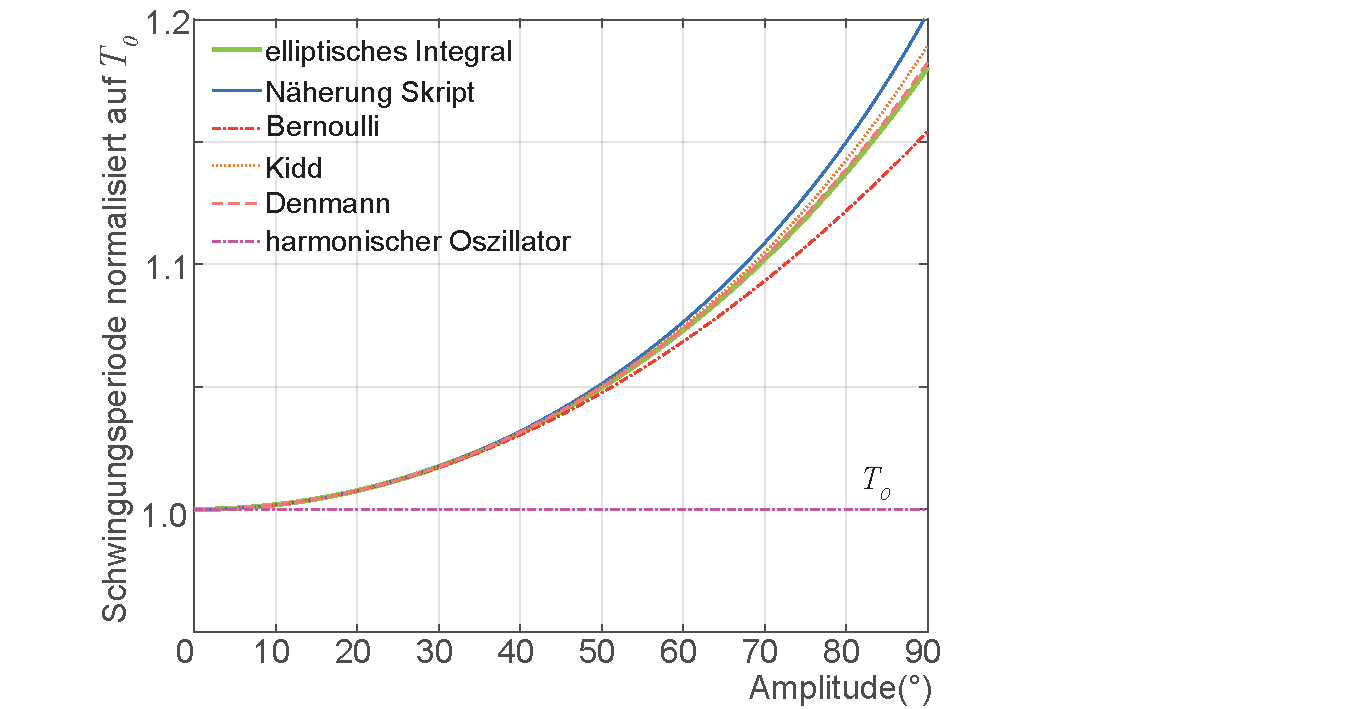
\includegraphics[width=\textwidth]{AnHarmonOsz01.pdf}
\caption[Schwingungsperiode des nichtlinearen Pendels als Funktion der Amplitude.]{Schwingungsperiode $T$ des nichtlinearen Pendels als Funktion der Amplitude $\theta_\text{A}$. L�sung nach \eqref{eq:bew_NLOsz12} sowie verschiedene N�herungsl�sungen aus der Literatur \cite{Hinrichsen2021} im Vergleich zur exakten und zur harmonischen L�sung. } \label{abb:bew_NLOsz01}
\end{figure}

\subparagraph{\textbf{Analytische Berechnung der Schwingungsperiode des nichtlinearen Pendels}}

Wir gehen hierbei �hnlich vor wie bei der Behandlung des Zweik�rperproblems (\kap{bew_ZKP_EEKP}).
Wir wissen, dass die Energie eine Erhaltungsgr��e der Bewegung ist, also gilt
\begin{align}
  E &= \text{const} = T+U = \frac{m}{2}l^2\dot{\theta}^2+\underbrace{m\,g\,l\,(1-\cos\theta)}_{\substack{U(\theta)}}  = m\,g\,l\,(1-\cos\theta_\text{A})  \nonumber \\
        &\rightarrow \frac{2\,(E-U(\theta))}{m\,l^2} = \lk \frac{\D\theta}{\D t}\rk^2~~\rightarrow~~\D t = \frac{\D \theta}{\sqrt{2\lek E - U(\theta) \rek/(m\,l^2)}}      \,. \label{eq:bew_NLOsz14}
\end{align}
Hierin ist $\theta_\text{A}$ die Amplitude des Pendels.
Wenn wir von $0$ bis $\theta_\text{A}$ integrieren, entspricht das einem Viertel  $T_\text{P}/4$  der Schwingungsperiode
	\begin{align}
			\frac{T_\text{P}}{4} = \int_{0}^{\frac{T_\text{P}}{4}} \D t = \bigintsss_{0}^{\theta_\text{A}} {\frac{\D \theta'}{\sqrt{\frac{2E-2U(\theta')}{m\,l^2}}}} = \sqrt{\frac{l}{2g}} \bigintsss_{0}^{\theta_\text{A}}\frac{\D \theta'}{\sqrt{\cos\theta'-\cos\theta_\text{A}}} \,. \label{eq:bew_NLOsz15}
	\end{align}
Mit $\cos x = 1-2\sin^2\frac{x}{2}$ erhalten wir
	\begin{align}
			\frac{T_\text{P}}{4} = \frac{1}{2}\sqrt{\frac{l}{g}} \bigintsss_{0}^{\theta_\text{A}}\frac{\D \theta'}{\sin\frac{\theta_\text{A}}{2}\sqrt{1-\bigg[\sin\frac{\theta'}{2} / \sin\frac{\theta_\text{A}}{2}\bigg]^2}}~. \label{eq:bew_NLOsz16}
	\end{align}
Unter Verwendung der Substitutionen 
    \begin{align*}
                z = \sin\frac{\theta'}{2} / k ~~~ \text{mit} ~~k = \sin\frac{\theta_\text{A}}{2}~~~\text{und} ~~~\D z = \frac{1}{2k}\cos\frac{\theta'}{2} \,\d \theta'  = \frac{1}{2k} \sqrt{1-k^2\,z^2} \,\D \theta' 
    \end{align*}
erhalten wir:
    \begin{align*}
                T_\text{P} = 4 \bigintsss_{0}^1 \frac{\D z}{\sqrt{(1-z^2)\,(1-k^2\,z^2)}} \,.
    \end{align*}
Mit der finalen Substitution $z = \sin\theta$ und der Periode des harmonischen Oszillators $2\pi\sqrt{l/g} = T_0 $
erhalten wir schlie�lich
    \begin{align}
                    T_\text{P} &= T_0 \frac{2}{\pi} \bigintsss_{0}^{\frac{\pi}{2}} \frac{\D\theta}{\sqrt{1-k^2\,\sin^2\theta}} = T_0 \frac{2}{\pi}\: \textbf{\textit{K}}(k)\: =\: T_0 \frac{2}{\pi}\: \textbf{\textit{K}}(\sin\frac{\theta_\text{A}}{2}) \,. \label{eq:bew_NLOsz17}
    \end{align}
    Hier ist $\textbf{\textit{K}}(k)$ das tabellierte \textit{vollst�ndige elliptische Integral erster Art}\index{Integral!elliptisches|textbf} \cite{Olver1992, Gradshteyn1980}, das nat�rlich auch numerisch mit \matlab{} berechnet werden kann \bzw dort auch als Funktion hinterlegt ist.

\subparagraph{\textbf{Methode der St�rungsrechnung zur Berechnung der Dynamik des nichtlinearen Pendels}}\index{St�rungsrechnung}

Gleichung \eqref{eq:bew_NLOsz17} ist gut geeignet, um eine Abh�ngigkeit der Schwingungsperiode von der Amplitude zu berechnen, siehe auch \figref{bew_NLOsz01}. 
Wir wollen nun noch die zeitliche Dynamik $\theta(t)$ des Systems betrachten.
Wir k�nnen diese nat�rlich aus 
\begin{align}
\ddot{\theta} + {\omega_0}^2 \sin\theta = 0  \label{eq:bew_NLOsz18}
\end{align}
numerisch berechnen oder L�sung \eqref{eq:bew_NLOsz03} benutzen mit $A_1 = \theta_\text{A}$ und $A_3$ gem�� \eqref{eq:bew_NLOsz07}.
Beide L�sungsvarianten sind im \mscr{} \mlbewref{AnHarmonOszillator02.m} ausgef�hrt und in \figref{bew_NLOsz02} auch im Vergleich zur harmonischen N�herung dargestellt.
Wie man erkennt, ist diese nur bis $\theta_\text{A} \approx 15\degree$ gut, wohingegen die N�herungsl�sungen auch noch bei $85 \degree$ brauchbare Ergebnisse liefern
(\figref{bew_NLOsz02}). Entwickeln wir die nichtlineare Schwingungsgleichung \eqref{eq:bew_NLOsz18} nach Potenzen von $\theta$ unter Benutzung der Abk�rzung $\Omega = \omega t$ und der Beziehung 
	\[\frac{\D }{\D t} \theta = \frac{\D \theta}{\D \Omega} \frac{\D \Omega}{\D t} = \theta' \, \omega\,,
\]
erhalten wir in der ersten nichtlinearen Ordnung die folgende zu Gleichung \eqref{eq:bew_NLOsz02} �quivalente DGL%
\footnote{Eine Differentialgleichung vom Typ $A\,y'' + B\,y + C\,y^3 = 0$ wird in der Literatur \cite{Kuypers2012} h�ufig als Duffing-DGL bezeichnet.}:
\begin{equation}
    \omega^2 \theta''(\Omega) + {\omega_0}^2 \theta(\Omega) - \kappa_3 \theta^3(\Omega) = 0~~~\text{mit}~~\kappa_3 = \frac{1}{6} {\omega_0}^2 \,.
    \label{eq:bew_StoerRe02}
\end{equation}
Wir wollen diese mit der Methode der St�rungsrechnung l�sen. Diese Methode wird in der Physik sehr h�ufig verwendet und wir werden ihr noch mehrmals begegnen.
F�r die L�sung der Differentialgleichungen \eqref{eq:bew_StoerRe02} betrachten wir die L�sung $\theta(\Omega)$ als zusammengesetzt aus der L�sung der linearen DGL $\theta_0(\Omega)$ und einem Zusatz, der aus der nichtlinearen St�rung $\sum\nolimits_i \kappa_i \theta^i$ folgt.
Ebenso betrachten wir die Schwingungsfrequenz $\omega$ als zusammengesetzt aus der L�sung f�r den linearen Fall $\omega_0$ und entsprechenden Zusatztermen.
Wir machen deshalb folgenden st�rungstheoretischen Ansatz, wobei wir f�r das nichtlineare Pendel nur die ungeraden Terme mitnehmen wollen\footnote{Die Rechnung f�r einen asymmetrischen Oszillator ist nat�rlich v�llig analog mit den zus�tzlichen geraden Termen.}:
\begin{align}
    \theta(\Omega) &= \theta_0(\Omega) + \kappa_3 \,\theta_1(\Omega) + {\kappa_3}^2 \,\theta_2(\Omega) + \ldots \nonumber \\
    \omega &= \omega_0 + \kappa_3 \,\omega_1 + {\kappa_3}^2 \,\omega_2 + \dots
    \label{eq:bew_StoerRe01}
\end{align}
Wir haben also angenommen, dass sich sowohl die L�sung selbst als auch die Eigenfrequenz des Pendels in Zusatztermen nach Potenzen der St�rungen darstellen lassen.
Wir setzen dies in \eqref{eq:bew_StoerRe02} ein und ordnen das Ergebnis nach Termen in Potenzen von $\kappa_3$, wobei jeder Term f�r sich verschwinden muss, da die Gleichung ja f�r alle Zeiten erf�llt sein muss:
%\begin{enumerate}[${\kappa_3}^1$:]
%    \setcounter{enumi}0
%  \item
%    ${\omega_0}^2 {\theta_0}'' + {\omega_0}^2 \theta_0 = 0 \label{eq:bew_StoerRe03a}$ \\
%  \item
%    ${\omega_0}^2 {\theta_1}'' + {\omega_0}^2 \theta_1 = {\theta_0}^3 - 2 \omega_0 \omega_1 {\theta_0}'' = 0  \label{eq:bew_StoerRe03b}$ \\
%  \item
%    ${\omega_0}^2 {\theta_2}'' + {\omega_0}^2 \theta_2 = 3 {\theta_0}^2 \theta_1 - ({\omega_1}^2 + 2\omega_0 \omega_2) {\theta_0}'' - 2 \omega_0 \omega_1 {\theta_1}''.$
%    \label{eq:bew_StoerRe03c}     
%\end{enumerate}
\begin{align}
    {\kappa_3}^0 :\quad &{\omega_0}^2 {\theta_0}'' + {\omega_0}^2 \theta_0 = 0 \label{eq:bew_StoerRe03a} \,,\\
    {\kappa_3}^1 :\quad &{\omega_0}^2 {\theta_1}'' + {\omega_0}^2 \theta_1 = {\theta_0}^3 - 2 \omega_0 \omega_1 {\theta_0}'' \,, \label{eq:bew_StoerRe03b} \\
    {\kappa_3}^2 :\quad &{\omega_0}^2 {\theta_2}'' + {\omega_0}^2 \theta_2 = 3 {\theta_0}^2 \theta_1 - ({\omega_1}^2 + 2\omega_0 \omega_2) {\theta_0}'' - 2 \omega_0 \omega_1 {\theta_1}''.
    \label{eq:bew_StoerRe03c}     
\end{align}
Man erkennt, dass die Gleichungen f�r die $\theta_i$ jeweils als Differentialgleichungen eines harmonischen Oszillators betrachtet werden k�nnen, die in den h�heren Ordnungen $\theta_i$ jeweils durch die niedrigeren Ordnungen angetrieben werden, also $\theta_1$ durch $\theta_0$, $\theta_2$ durch $\theta_1, \theta_0$ \usW
Die Anfangsbedingungen zur L�sung von \eqref{eq:bew_StoerRe02} sollen jeweils durch die nullte N�herung erf�llt werden, \dh
\begin{align}
    \theta_0 &= \theta_0(0) = \theta_A \qquad \text{(Anfangsamplitude)} \nonumber \\
    \dot{\theta_0} &= \dot{\theta_0}(0) = \dot{\theta_A} = 0 ~.
\end{align}
Damit sind alle $\theta_i(0)$ und $\dot{\theta_i}(0)$ f�r $i \geq 1$ gleich Null.
Die L�sung von \eqref{eq:bew_StoerRe03a} ergibt sich mit den Anfangsbedingungen zu
\begin{equation}
    \theta_0 = \theta_A \cos \Omega = \theta_A \cos \omega t \label{eq:bew_StoerRe04}~.
\end{equation} 
Setzen wir dies in \eqref{eq:bew_StoerRe03b} ein, erhalten wir f�r $\theta_1$ folgende DGL:
\begin{equation}
    {\omega_0}^2 {\theta_1}'' + {\omega_0}^2 \theta_1 = \lk \frac{3}{4} {\theta_A}^3 + 2 \omega_1 \omega_0 \theta_A \rk \cos \Omega + \frac{1}{4} {\theta_A}^3 \cos 3 \Omega
    \label{eq:bew_StoerRe05}~.
\end{equation}
Damit $\theta_1$ eine stabile Schwingungsl�sung ist, \dh nicht �ber alle Ma�en ansteigt,
muss der Term in der Klammer verschwinden%
\footnote{Der Beweis hierf�r sei als �bung empfohlen, auch eine numerische Rechnung f�r eine nichtverschwindende Klammer ist sehr instruktiv.},
woraus
\begin{equation*}
    \omega_1 = -\frac{3}{8} \frac{{\theta_A}^2}{\omega_0} \label{eq:bew_StoerRe06a}
\end{equation*}
folgt und somit f�r die Frequenz
\begin{align}
    \omega &= \omega_0 + \kappa_3 \omega_1 \nonumber = \omega_0 \lk 1 - \kappa_3 \frac{3}{8} \frac{{\theta_A}^2}{{\omega_0}^2} \rk = \omega_0 \lk 1 - \frac{ {\theta_A}^2}{16} \rk \,. \label{eq:bew_StoerRe06a}
\end{align}
erhalten.
Au�erdem ergibt sich daraus
\begin{equation}
    \theta_1 = \frac{1}{32} \frac{{\theta_A}^3}{{\omega_0}^2} (\cos\omega t - \cos 3 \omega t) \label{eq:bew_StoerRe06b}~.
\end{equation}
Wir sehen also, dass in erster N�herung nicht nur die Frequenz $\omega_0$ um $\kappa_3 \omega_1$ verschoben wurde, sondern dass auch in der Zeitdynamik ein Term $\kappa_3 \theta_1$ mit einer Oberschwingung bei $3 \omega$ hinzukommt.
Das Ergebnis ist somit sehr �hnlich dem, welches wir aus dem harmonischen Ansatz (vgl. \eqref{eq:bew_NLOsz12}) erhalten hatten.
Wir k�nnen jetzt noch die n�chste N�herungsordnung angehen.
Mit \eqref{eq:bew_StoerRe03c} und den trigonometrischen Identit�ten $\cos^3x = (3 \cos x + \cos 3x)/4$ sowie $\cos^2x = (\cos x + 2 \cos 3x + \cos 5x)/4$ findet man nach etwas Algebra
\begin{equation}
    {\omega_0}^2 \theta_2 '' + {\omega_0}^2 \theta_2
    = \lk \frac{21}{128} \frac{{\theta_A}^5}{{\omega_0}^2} + 2 \omega_0 \omega_2 \theta_A \rk \cos \Omega
    + \lk \frac{24}{128} \frac{{\theta_A}^5}{{\omega_0}^2} \rk \cos 3 \Omega
    + \lk - \frac{3}{128} \frac{{\theta_A}^5}{{\omega_0}^2} \rk \cos 5 \Omega
    \label{eq:bew_StoerRe07}~.
\end{equation}
Man erkennt, dass die Beitr�ge in den Klammern mit der Zunahme der Frequenz im $\cos$-Term immer kleiner werden,
wobei der erste Klammerterm wieder Null sein muss, damit es eine stabile L�sung gibt.
Wir erhalten damit als Bedingung 
\begin{equation}
     \omega_2 = - \frac{21}{256} \frac{{\theta_A}^4}{{\omega_0}^3} \label{eq:bew_StoerRe8a}
\end{equation}
und daraus 
\begin{equation}
    \theta_2 = \frac{1}{1024} \frac{{\theta_A}^5}{{\omega_0}^4} \lk 23 \cos \omega t - 24\cos 3 \omega t \rk~.
\end{equation}
Insgesamt ergibt sich also bis zur zweiten Ordnung der St�rungsrechnung
\begin{subequations}
\begin{align}
    \theta &= \theta_0 + \kappa_3 \theta_1 + {\kappa_3}^2 \theta_2 \nonumber \\
    &= \theta_A \lk 1 + \frac{{\theta_A}^2}{192} + \frac{23}{1024}\frac{{\theta_A}^4}{36}\rk \cos\omega t - \frac{{\theta_A}^3}{6} \lk \frac{1}{32} + \frac{{\theta_A}^2}{256} \rk \cos3\omega t + \frac{1}{1024} \frac{{\theta_A}^5}{36} \cos5\omega t \label{eq:bew_StoerRe09a} \\
		\text{und}  \nonumber \\
    \omega &= \omega_0 \lk 1 - \frac{1}{16} {\theta_A}^2 - \frac{7}{3072}{\theta_A}^4 \rk
    \label{eq:bew_StoerRe09b}~.
\end{align}
\end{subequations}
Es ist interessant, dass die Korrekturterme nur von der Anfangsamplitude und weiteren Konstanten abh�ngen, nicht aber von der Pendell�nge.
In \figref{bew_NLOsz02} haben wir auch L�sung \eqref{eq:bew_StoerRe09a} mit der numerischen L�sung der vollst�ndigen Pendelgleichung \eqref{eq:bew_NLOsz18} verglichen.

\begin{figure}
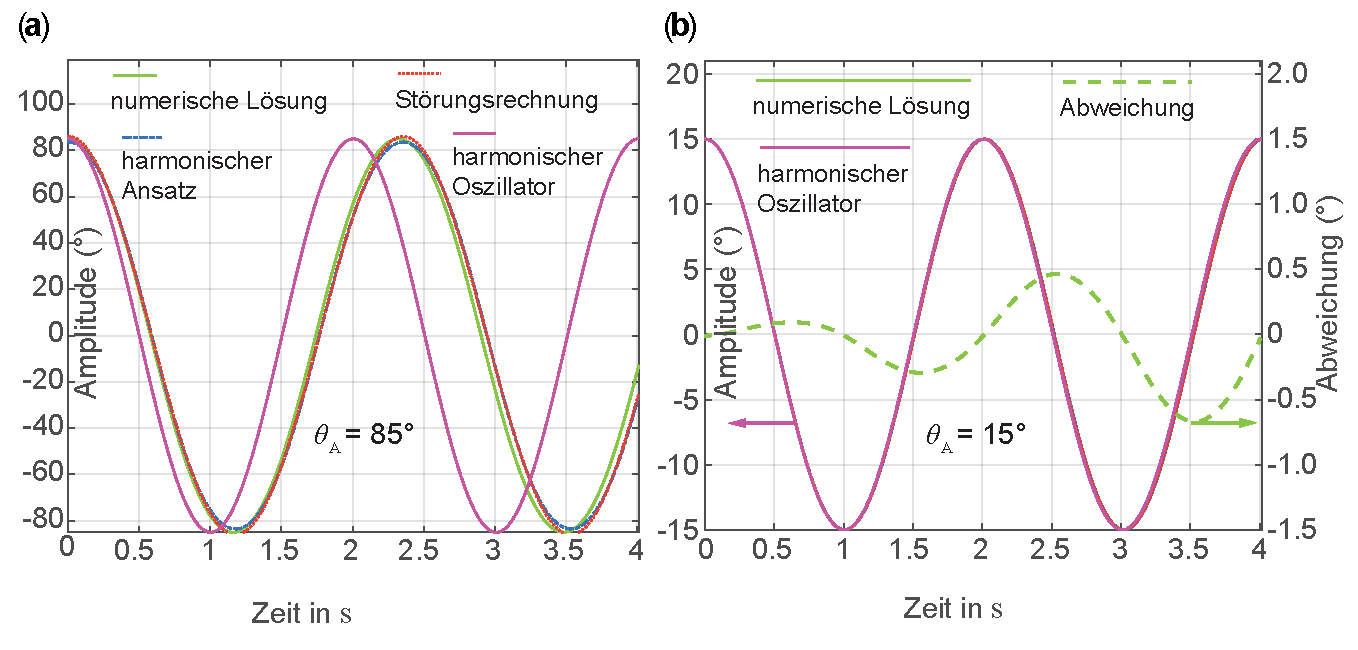
\includegraphics[width=\textwidth]{AnHarmonOsz02.pdf}
\caption[Schwingungsverhalten des nichtlinearen Pendels.]{Schwingungsverhalten $\theta(t)$ des nichtlinearen Pendels f�r verschiedene Amplituden $\theta_\text{A}$. Gezeigt sind verschiedene N�herungsl�sungen im Vergleich zur numerischen L�sung. \fa f�r Auslenkung $85\degree$ \fb f�r Auslenkung $85\degree$.} \label{abb:bew_NLOsz02}
\end{figure}


\subsubsection{Das Zykloidenpendel und die Brachistochrone} \index{Brachistochrone}\index{Pendel!Zykloidenpendel}\label{kap:bew_pendulum_zykl}

Wir hatten im vorhergehenden Kapitel gesehen, dass bei einem Fadenpendel die Schwingungsperiode von der Amplitude abh�ngt.
Da stellt sich die Frage, ob es eine M�glichkeit gibt, ein Pendel so zu konstruieren, dass die Schwingungsperiode unabh�ngig von der Auslenkung ist.\footnote{Dieses Problem war f�r die Uhrmacher des 17.~Jahrhunderts, \ua auch f�r Huygens, ein ganz reales.} Konkret sucht man also die Kurve, auf der sich ein Massepunkt mit konstanter Frequenz hin- und herbewegt, und zwar unabh�ngig von seiner maximalen Auslenkung.
Eine solche Kurve nennt man \emph{Tautochrone}.\footnote{Aus dem Griechischen f�r \textit{selbe Zeit}.}\index{Tautochrone}\\
Eng verwandt mit diesem Problem ist die Suche nach der Kurve im homogenen Schwerefeld, auf der ein sich reibungsfrei bewegender Massepunkt nur unter dem Einfluss der Gravitationskraft am schnellsten von einem Anfangspunkt $(x_\text{A},z_\text{A})$ zu einem gleich hoch oder tiefer gelegenen Endpunkt $(x_\text{E},z_\text{E})$ gelangt, wobei der Tiefpunkt der Bahn $(x_\text{T},z_\text{T})$ tiefer liegen kann als der Endpunkt.
Das Brachistochronenproblem wurde in einem Wettstreit zwischen den ziemlich verfeindeten Br�dern Jakob und Johann Bernoulli%
\footnote{Jakob Bernoulli (1655--1705) war ein Schweizer Mathematiker und Physiker, der wesentlich zur Entwicklung der Wahrscheinlichkeitstheorie sowie zur Variationsrechnung und zur Untersuchung von Potenzreihen beigetragen hat.\\
Johann Bernoulli (1667--1748) war Schweizer Mathematiker und Arzt und der j�ngere Bruder von Jakob Bernoulli.
Er arbeitete unter anderem auf dem Gebiet der Reihen und Differentialgleichungen und spielte eine wichtige Rolle bei der Entwicklung der Variationsrechnung.
So stellte er 1696 das Problem der Brachistochrone, das 1697 von ihm, seinem Bruder (sehr zu Johanns �rger), Newton (anonym) und Leibniz gel�st wurde.
Zur Geschichte und zu verschiedenen Ans�tzen zur L�sung des Brachistochronenproblems gibt es eine Reihe sch�ner Darstellungen \ua in \cite{Nahin2003, Shafer2007, Resch2018}.}%
\indexp{Bernoulli, Jakob}\indexp{Bernoulli, Johann} gel�st.
Damit wurden auch die Grundlagen der \emph{Variationsrechnung}\index{Variationsrechnung} geschaffen.
Wir wollen uns deshalb die Idee der Variationsrechnung zun�chst bei der Berechnung der Brachistochrone anschauen und das Ergebnis dann f�r die Beantwortung der Frage nach dem Pendel mit amplitudenunabh�ngiger Schwingungsperiode benutzen.

\subparagraph{\textbf{Brachistochrone}}

Die Kurve, auf der sich der Massepunkt bewegen soll, sei durch $z = f (x)$ gegeben (\figref{bew_Zykloid01}).
Die Lagrange-Funktion mit der unabh�ngigen Variablen $x$ ist dann gegeben durch
\begin{align}
	\mathcal{L} = \frac{m}{2} \lk\dot{x}^2 + \dot{z}^2 \rk + m\,g\,z = \frac{m}{2} \lk 1 + \lek f'(x)\rek^2 \rk \dot{x}^2 - m\,g\,f(x) \,. \label{eq:bew_Zykloid01}
\end{align}
Hierbei haben wir benutzt:
	\[\dot{z}= \frac{\D z}{\D t} = \frac{\D z}{\D x} \frac{\D x}{\D t} = z'(x)\,\dot{x} = f'(x)\,\dot{x} \,.
	\]
Ferner schreiben wir die Anfangs- und Randbedingungen wie folgt:
	\[ z(0) = z_\text{A} = 0\,,\,z(T) = z_\text{E}\,,\, x(T) = x_\text{E},\, \dot{z}(0) = \dot{z}_\text{A} =\dot{x}(0) = \dot{x}_\text{A} = 0\,. 
\]
Entgegen der �blichen Konvention lassen wir $z$ in die negative Richtung laufen, ersetzen also $z \rightarrow  -z$ (\figref{bew_Zykloid01}).
So geschrieben ist die Lagrange-Funktion in unserem Fall nur noch von der Funktion $f(x)$ bzw. $f'(x)$ abh�ngig, k�nnte im allgemeinen Fall aber auch noch explizit von $x$ abh�ngen.
Wir k�nnen Bewegungsgleichung \eqref{eq:bew_Zykloid01} sofort integrieren, da Energieerhaltung (siehe \eqref{eq:bew_Hamilton_Fkt}) gilt:
\begin{align}
	E = \dot{x} \frac{\partial \mathcal{L}}{\partial \dot{x}} -  \mathcal{L} = \frac{m}{2} \lk 1 + \lek f'(x)\rek^2 \rk \dot{x}^2 + m\,g\,f(x) = m\,g\,f(x_\text{A})\,. \label{eq:bew_Zykloid02}
\end{align}
Hierbei haben wir $E(t_\text{A}) = m\,g\,f(x_\text{A})$ angenommen.
Wir k�nnen \eqref{eq:bew_Zykloid02} durch Trennung der Variablen $x$ und $t$ in impliziter Form l�sen und erhalten
\begin{align}
	T &= \int_{t_\text{A}}^{t_\text{E}}\, \D t = \bigintsss_{x_\text{A}}^{x_\text{E}} \sqrt \frac{1+\lek f'[x]\rek^2}{2g\,\lk f(x_\text{A}) - f(x) \rk}\, \D x  = \bigintsss_{x_\text{A}}^{x_\text{E}} \mathcal{F}\lk f(x)\,,f'(x) \rk \D x \,. \label{eq:bew_Zykloid03}
\end{align}
Im \mscr{} \mlbewref{Brachistochrone.m} haben wir die Zeiten $T_i$ als Funktion verschiedener Kurven $f_i(x)$ berechnet und in \figref{bew_Zykloid02} dargestellt.
Man erkennt, dass im dargestellten Fall weder die direkte Verbindung noch der Kreisbogen (wie von Galilei angenommen) die k�rzeste "`Fallzeit"' ergeben.%
\footnote{Wir weisen darauf hin, dass das Integral in \eqref{eq:bew_Zykloid03} ein sogenanntes uneigentliches Integral ist, da $f(0) = 0$ ist und dar�ber hinaus die Tangente an $f$ bei $x=0$ senkrecht steht und $f'$ damit unendlich gro� wird. Der Fall $x_\text{A} = x_\text{E}=0$ muss daher im Grenz�bergang gesondert betrachtet werden.}
Wir suchen nun bei festen Endpunkten ($x_\text{A},x_\text{E})$ die Kurve oder Kurven $z(x) = f_\text{min}(x)$, f�r die die Zeit $T_{\min}$ minimal wird.
$\mathcal{F}\lk f(x)\,, f'(x) \rk$ in \eqref{eq:bew_Zykloid03} ist ein sogenanntes \emph{Funktional}\index{Funktional}, \dh eine Funktion einer Funktion.
Es handelt sich um ein sogenanntes \emph{Variationsproblem}\index{Variationsproblem}.
F�r dieses kann man zeigen \cite{Schmutzer2005, Greiner2003, Suesskind2014}, dass das Integral
\begin{align}
  I &= \bigintsss_{x_\text{A}}^{x_\text{E}} \mathcal{F}\lk f(x), f'(x) \rk \D x = \bigintsss_{x_\text{A}}^{x_\text{E}} \mathcal{F}\lk z(x), z'(x) \rk \D x \label{eq:bew_Zykloid05}
\end{align}
nur dann ein Minimum (Extremum) annimmt, wenn folgende Gleichung erf�llt ist:
\begin{align}
		\frac{\D}{\D x} \frac{\partial \mathcal{F}(z,z')}{\partial z'} - \frac{\partial \mathcal{F}(z,z')}{\partial z} = 0 . \label{eq:bew_Zykloid06}
\end{align}

\begin{figure}
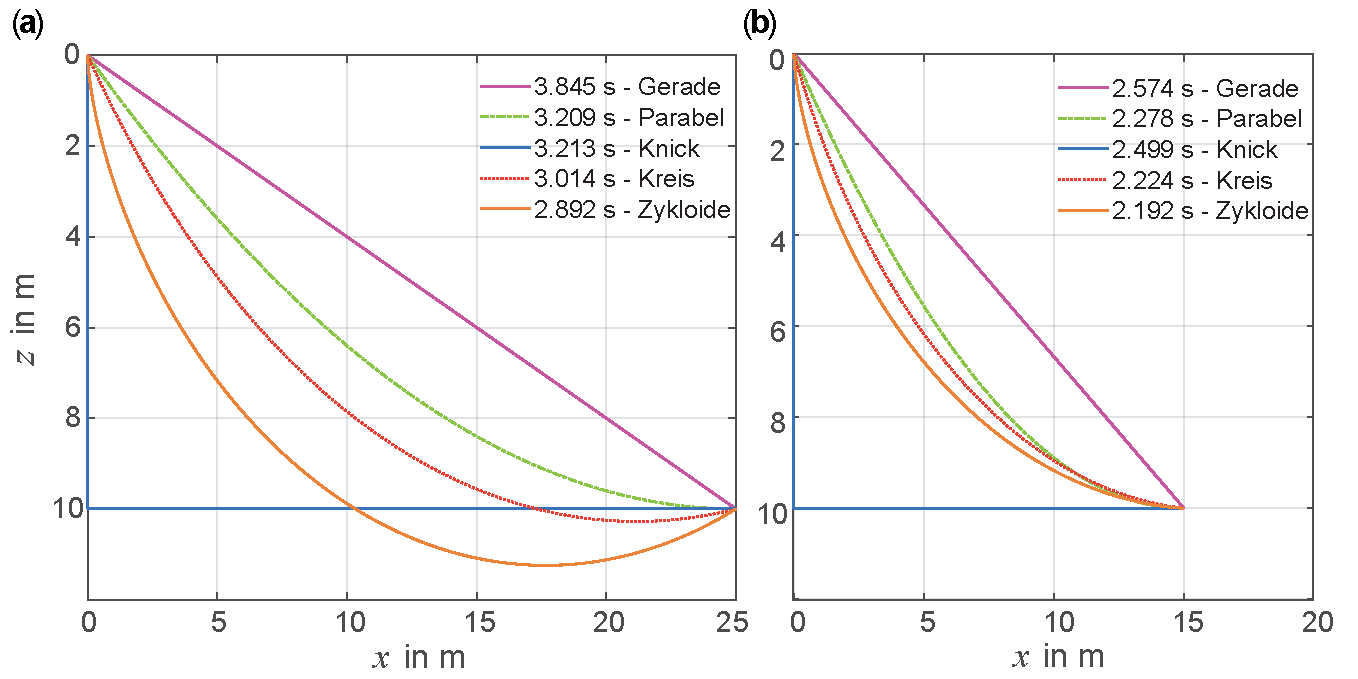
\includegraphics[width=\textwidth]{Zykloide01.pdf}
\caption[Verschiedene Fallkurven und deren Durchlaufzeiten.]{Fallkurven f�r eine Fallh�he von jeweils $\SI{10}{\metre}$ und deren Durchlaufzeiten f�r \fa eine Basisl�nge von $\SI{25}{\metre}$ und \fb eine Basisl�nge von $\SI{15}{\metre}$.} \label{abb:bew_Zykloid01}
\end{figure}

Diese Gleichung hei�t \emph{Euler-Lagrange-Gleichung}\index{Euler-Lagrange-Gleichung} und hat gro�e �hnlichkeit mit der Lagrange-Gleichung 2.\ Art
\eqref{eq:bew_LagrangeGl_II}, nur ist $\mathcal{F}$ hier ein \emph{Funktional} und $z=z(x)$ eine Funktion.%
\footnote{Die gleiche Struktur von \eqref{eq:bew_LagrangeGl_II} und \eqref{eq:bew_Zykloid06} ist nat�rlich nicht zuf�llig, sondern tief in der Struktur der Mechanik begr�ndet.
Wir empfehlen zur Vertiefung \cite{Schmutzer2005, Simonyi2004, Suesskind2014}.}
Damit k�nnen wir nun das Problem der Brachistochrone l�sen.
Wir schreiben f�r $\mathcal{F}\lk z(x)\,,z'(x)\rk$ in \eqref{eq:bew_Zykloid03} kurz als
\begin{align}
   \mathcal{F} =& \sqrt \frac{1+z'^2}{2g\, z}\,,  \label{eq:bew_Zykloid08}
\end{align}
womit man aus \eqref{eq:bew_Zykloid06} �ber folgende Schritte
\begin{align*}
    0 &=\frac{\D}{\D x}\,\frac{\d \mathcal{F}}{\d z'} - \frac{\d \mathcal{F}}{\d z}\, ~~~~ \Bigg|\,\cdot z'\pm z''\,\frac{\d \mathcal{F}}{\d z'} \\
    &= z'\,\frac{\D}{\D x}\,\frac{\d \mathcal{F}}{\d z'} - z'\,\frac{\d \mathcal{F}}{\d z} + z''\,\frac{\d \mathcal{F}}{\d z'} - z''\,\frac{\d \mathcal{F}}{\d z'} \\
    &= -\underbrace{\lk z'\,\frac{\d \mathcal{F}}{\d z}+z''\,\frac{\d \mathcal{F}}{\d z'}\rk}_{\frac{\D}{\D x} \mathcal{F}}+\underbrace{\lk z''\,\frac{\d \mathcal{F}}{\d z'}+z'\,\frac{\D}{\D x}\,\frac{\d \mathcal{F}}{\d z'}\rk}_{\frac{\D}{\D x}\lk z'\,\frac{\d \mathcal{F}}{\d z'}\rk}\\
    &= \frac{\D}{\D x}\,\lk z'\,\frac{\d \mathcal{F}}{\d z'}-\mathcal{F}\rk \\
    \intertext{als Zwischenergebnis}
    \Rightarrow \,& z'\,\frac{\d \mathcal{F}}{\d z'}-\mathcal{F} = \mathrm{const} = \hat{A}
\end{align*}
erh�lt. Mit \eqref{eq:bew_Zykloid08} ergibt sich daraus �ber 
\begin{align*}
    z'\,\frac{\d \mathcal{F}}{\d z'} &= \frac{1}{\sqrt{2g\,z}}\,\frac{{z'}^2}{\sqrt{1+{z'}^2}}\\
    \rightarrow \hat{A} &= z'\,\frac{\d \mathcal{F}}{\d z'}-\mathcal{F} =\frac{1}{\sqrt{2g\,z}}\lek \frac{{z'}^2}{\sqrt{1+{z'}^2}}-\sqrt{1+{z'}^2}\rek   =  \frac{1}{\sqrt{2g\,z}} \frac{{z'}^2+1-{z'}^2}{\sqrt{1+{z'}}}\, 
\end{align*}
schlie�lich die wichtige Beziehung 
\begin{align}
 1 + z'^2 = \frac{1}{\hat{A}^2\,2g} \frac{1}{z} = \frac{A}{z} \,. \label{eq:bew_Zykloid09}
\end{align}
Nach Trennung der Variablen erhalten wir
\begin{align}
		    \pm \D x &= \sqrt{\frac{z}{A-z}}\,\D z \,. \label{eq:bew_Zykloid09a}
\end{align}
Dies ist eine Differentialgleichung f�r $z(x)$, die wir mit dem Ansatz $z = A\sin^2\widetilde{\varphi}$ und $\D z = 2A\,\sin\widetilde{\varphi}\,\cos\widetilde{\varphi}\,\D \widetilde{\varphi}$ l�sen k�nnen:
\begin{align*}
    \D x &= 2A\,\sqrt{\frac{\killA{A}\,\sin^2\widetilde{\varphi}}{\killA{A}\,\lk 1-\sin^2\widetilde{\varphi}\rk}}\,\sin\widetilde{\varphi}\,\cos\widetilde{\varphi}\,\D \widetilde{\varphi}\\
    &= 2A\,\sin^2\widetilde{\varphi}\,\D\widetilde{\varphi} = A\lk 1-\cos 2\widetilde{\varphi}\rk\,\D \widetilde{\varphi} \,.
\end{align*}
Die Integration ergibt
\begin{align*}
    x &= A\lk \widetilde{\varphi}-\frac{1}{2}\,\sin 2\widetilde{\varphi}\rk + B = \frac{A}{2}\,\lk 2\widetilde{\varphi} -\sin 2\widetilde{\varphi}\rk +B \,,
\end{align*}
worin $B$ eine durch die Anfangsbedingungen festgelegte Integrationskonstante ist, die wegen $x_\text{A}=0$ als Null erkannt wird. Wir betrachten nur die positive $x$-Richtung, setzen 
$ 2 \widetilde{\varphi} \rightarrow\, \varphi$ und  $ A/2\, \rightarrow\, A$ und erhalten
\begin{align}
		x = A\lk\varphi - \sin{\varphi}\rk ~~\text{und}~~ z = A\lk 1 - \cos{\varphi}\rk \,. \label{eq:bew_Zykloid11}
\end{align}
Das ist aber gerade die parametrisierte Darstellung einer \emph{Zykloiden}.\index{Zykloide}
Eine solche Kurve wird von einem Punkt beschrieben, der sich auf dem Rand eines Rades befindet,
das entlang der x-Achse abrollt ohne zu gleiten.
Dabei sind $\varphi$ der Rollwinkel und $A$ der Durchmesser des Rades (\figref{bew_Zykloid02}).%
\footnote{Genau betrachtet ist die hier abgeleitete Brachistochrone die Spiegelung einer Zykloiden an der $x$-Achse.
Durch unsere Wahl der $z$-Koordinate in negativer Richtung kommen wir aber wieder auf die �bliche Zykloidendarstellung in Parameterform.
Als �bung sei empfohlen zu zeigen, dass \eqref{eq:bew_Zykloid11} tats�chlich eine Zykloide beschreibt und $A$ dem Durchmesser des abrollenden Rades entspricht.}
Die Brachistochrone ist also durch eine Zykloide gegeben, deren Parameter $A$ und $\varphi_\text{max} = \varphi_\text{E} $ sich aus den Anfangs- und Randbedingungen bestimmen lassen.
Insbesondere ergibt sich $\varphi_\text{E} $ aus
\begin{align}
	\frac{x(T)}{z(T)} = \frac{x_\text{E}}{z_\text{E}} = \frac{\varphi_\text{E}-\sin\varphi_\text{E}}{1 - \cos\varphi_\text{E}} \,. \label{eq:bew_Zykloid12}
\end{align}
Gleichung \eqref{eq:bew_Zykloid12} l�sst sich bis auf Spezialf�lle (Tab. \ref{tab:bew_Zykloid01}) nur numerisch l�sen.

\begin{table}[h!]
  \centering
   \begin{tabular}{ | C{2cm} | C{2cm}| C{2cm} | L{2cm} |} 
      \hline
            \rule{0pt}{2pt} & &  & \\
             $x_\text{E}$ & $x_\text{E}/z_\text{E}$& $\varphi_\text{E}$ & \\
            \rule{0pt}{2pt} & &  & \\
      \hline
            \rule{0pt}{2pt} & &  & \\
             \SI{0.0}{\metre} & 0.0  & nicht definiert & freier Fall \\
             \SI{10.0}{\metre} & 1.0  & & Neigung 45$\degree$\\
             \SI{15.7}{\metre} & $\pi/2$  & $\pi$ &  \\
             \SI{25.0}{\metre} & 2.5  &  &  \\
             \SI{31.4}{\metre} & $\pi$  &   & \\
              $\infty$ & $\infty$ & $2\pi$ &  \\
            \rule{0pt}{2pt} & &  & \\
      \hline
    \end{tabular}
    \medskip
    \caption[Parameter einer Zykloiden.]{Parameter einer Zykloiden. Siehe auch \figref{bew_Zykloid02}.}
    \label{tab:bew_Zykloid01}
\end{table}

\begin{figure}
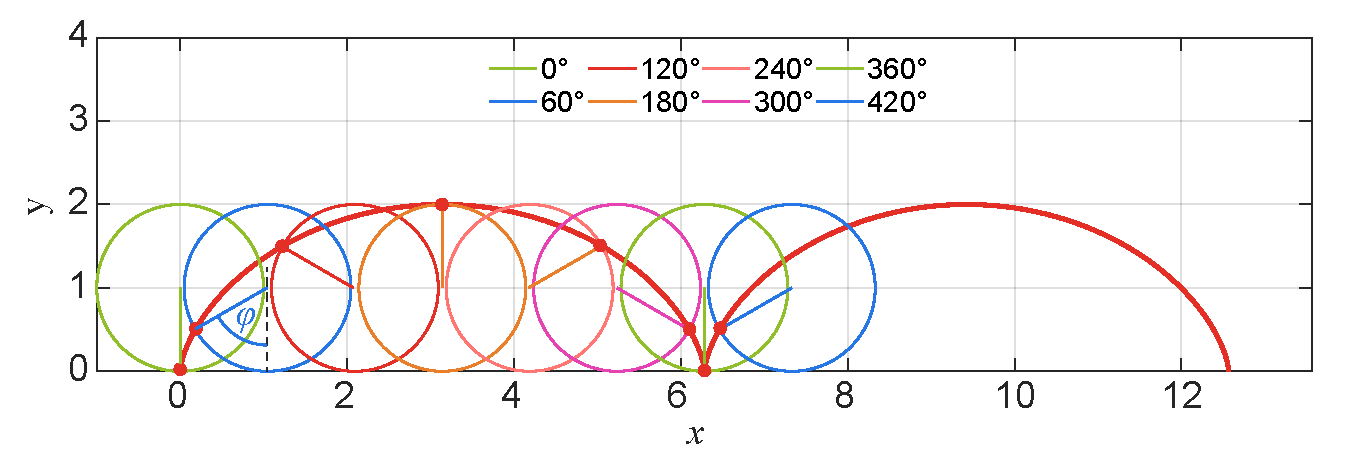
\includegraphics[width=\textwidth]{Zykloide02.pdf}%
\caption[Konstruktion einer Zykloiden.]{Konstruktion einer Zykloiden.} \label{abb:bew_Zykloid02}
\end{figure}

Wir k�nnen noch die gesamte Fallzeit entlang der Brachistochrone berechnen.
Wir starten mit Gleichung \eqref{eq:bew_Zykloid03} und formen diese leicht um:
\begin{align}
		T &= \bigintsss_{0}^{x_\text{E}} \sqrt{ \frac{ \lk\D x\rk^2 + \lk \D z\rk^2}{2g\,z} } \D x 
		   = \bigintsss_{0}^{\varphi_\text{E}} \sqrt {\frac{ A^2 \lk 1 - \cos\varphi \rk^2 + A^2 \lk \sin\varphi \rk^2}{2g\,A\lk 1 -\cos\varphi\rk} } \,\D \varphi \nonumber \\
		  &= \sqrt{\frac{A}{2g}}\bigintsss_{0}^{\varphi_\text{E}} \sqrt {\frac{ 1 - 2\cos\varphi  + \cos^2\varphi + \sin^2\varphi}{\lk 1 -\cos\varphi\rk} } \,\D \varphi \nonumber \\
                  &= \sqrt{\frac{A}{2g}}\bigintsss_{0}^{\varphi_\text{E}} \sqrt {\frac {2\,\lk 1 - \cos\varphi \rk}{\lk 1 -\cos\varphi \rk} } \,\D \varphi
		   = \sqrt{\frac{A}{g}}\bigintsss_{0}^{\varphi_\text{E}} \D \varphi = \sqrt{\frac{A}{g}}\,\varphi_\text{E} \,,\label{eq:bew_Zykloid13}
\end{align}
worin sich $A$ aus der \anf{Fallh�he} $z_\text{E}$ �ber $A = z_\text{E}/(1-\cos\varphi_\text{E})$ bestimmt und $0 < \varphi_\text{E} < 2\pi$ ist.\\
Eine sehr sch�ne Brachistochrone aus dem 18.~Jahrhundert ist heute im Museum Galileo in Florenz zu sehen (\figref{bew_Zykloid04}).
Dort kann man die Laufzeit einer Kugel im direkten Vergleich zur schiefen Ebene erfahren.
Es ist in diesem Zusammenhang auch eine interessante Frage, ob man bei Notfallrutschen am Flugzeug eine Brachistochrone nachbilden sollte.
Als �bung sei empfohlen, den m�glichen Zeitgewinn einer Brachistochrone-Notfallrutsche bei 500 Passagieren gegen�ber einer einfachen schiefen Ebene zu berechnen (\mscr{} \mlbewref{Brachistochrone.m}). 

\subparagraph{\textbf{Tautochrone, Zykloidenpendel}}

\begin{figure}
\begin{minipage}{\textwidth}
\leftfigure{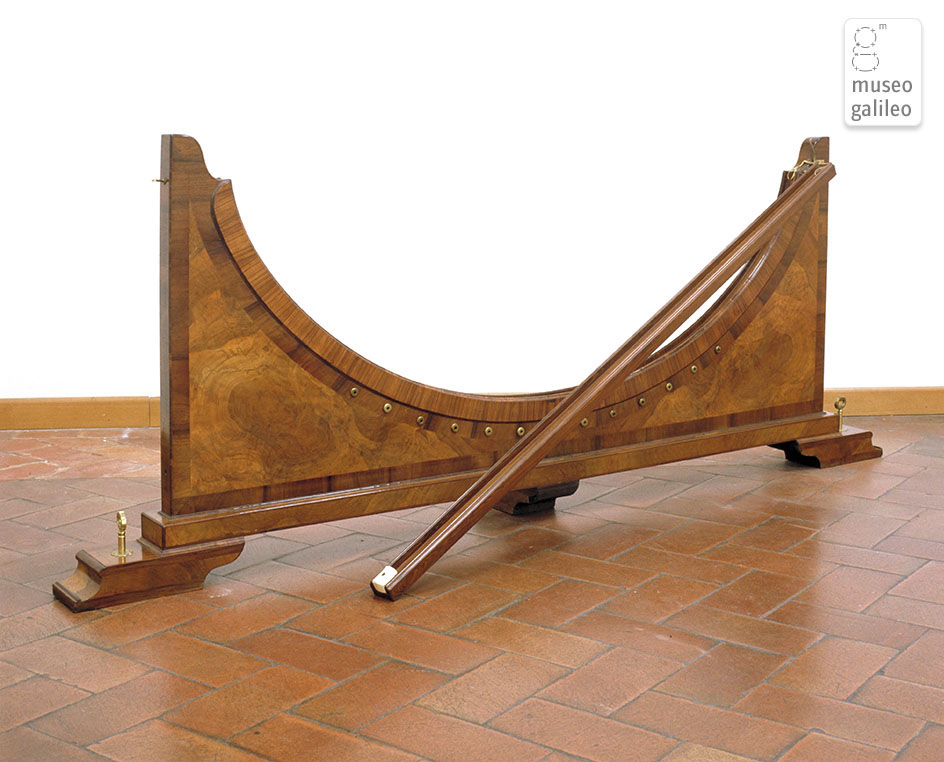
\includegraphics[width=0.5\textwidth]{Brachistochrone.jpg}}%
\hspace{\fill}
\rightfigure{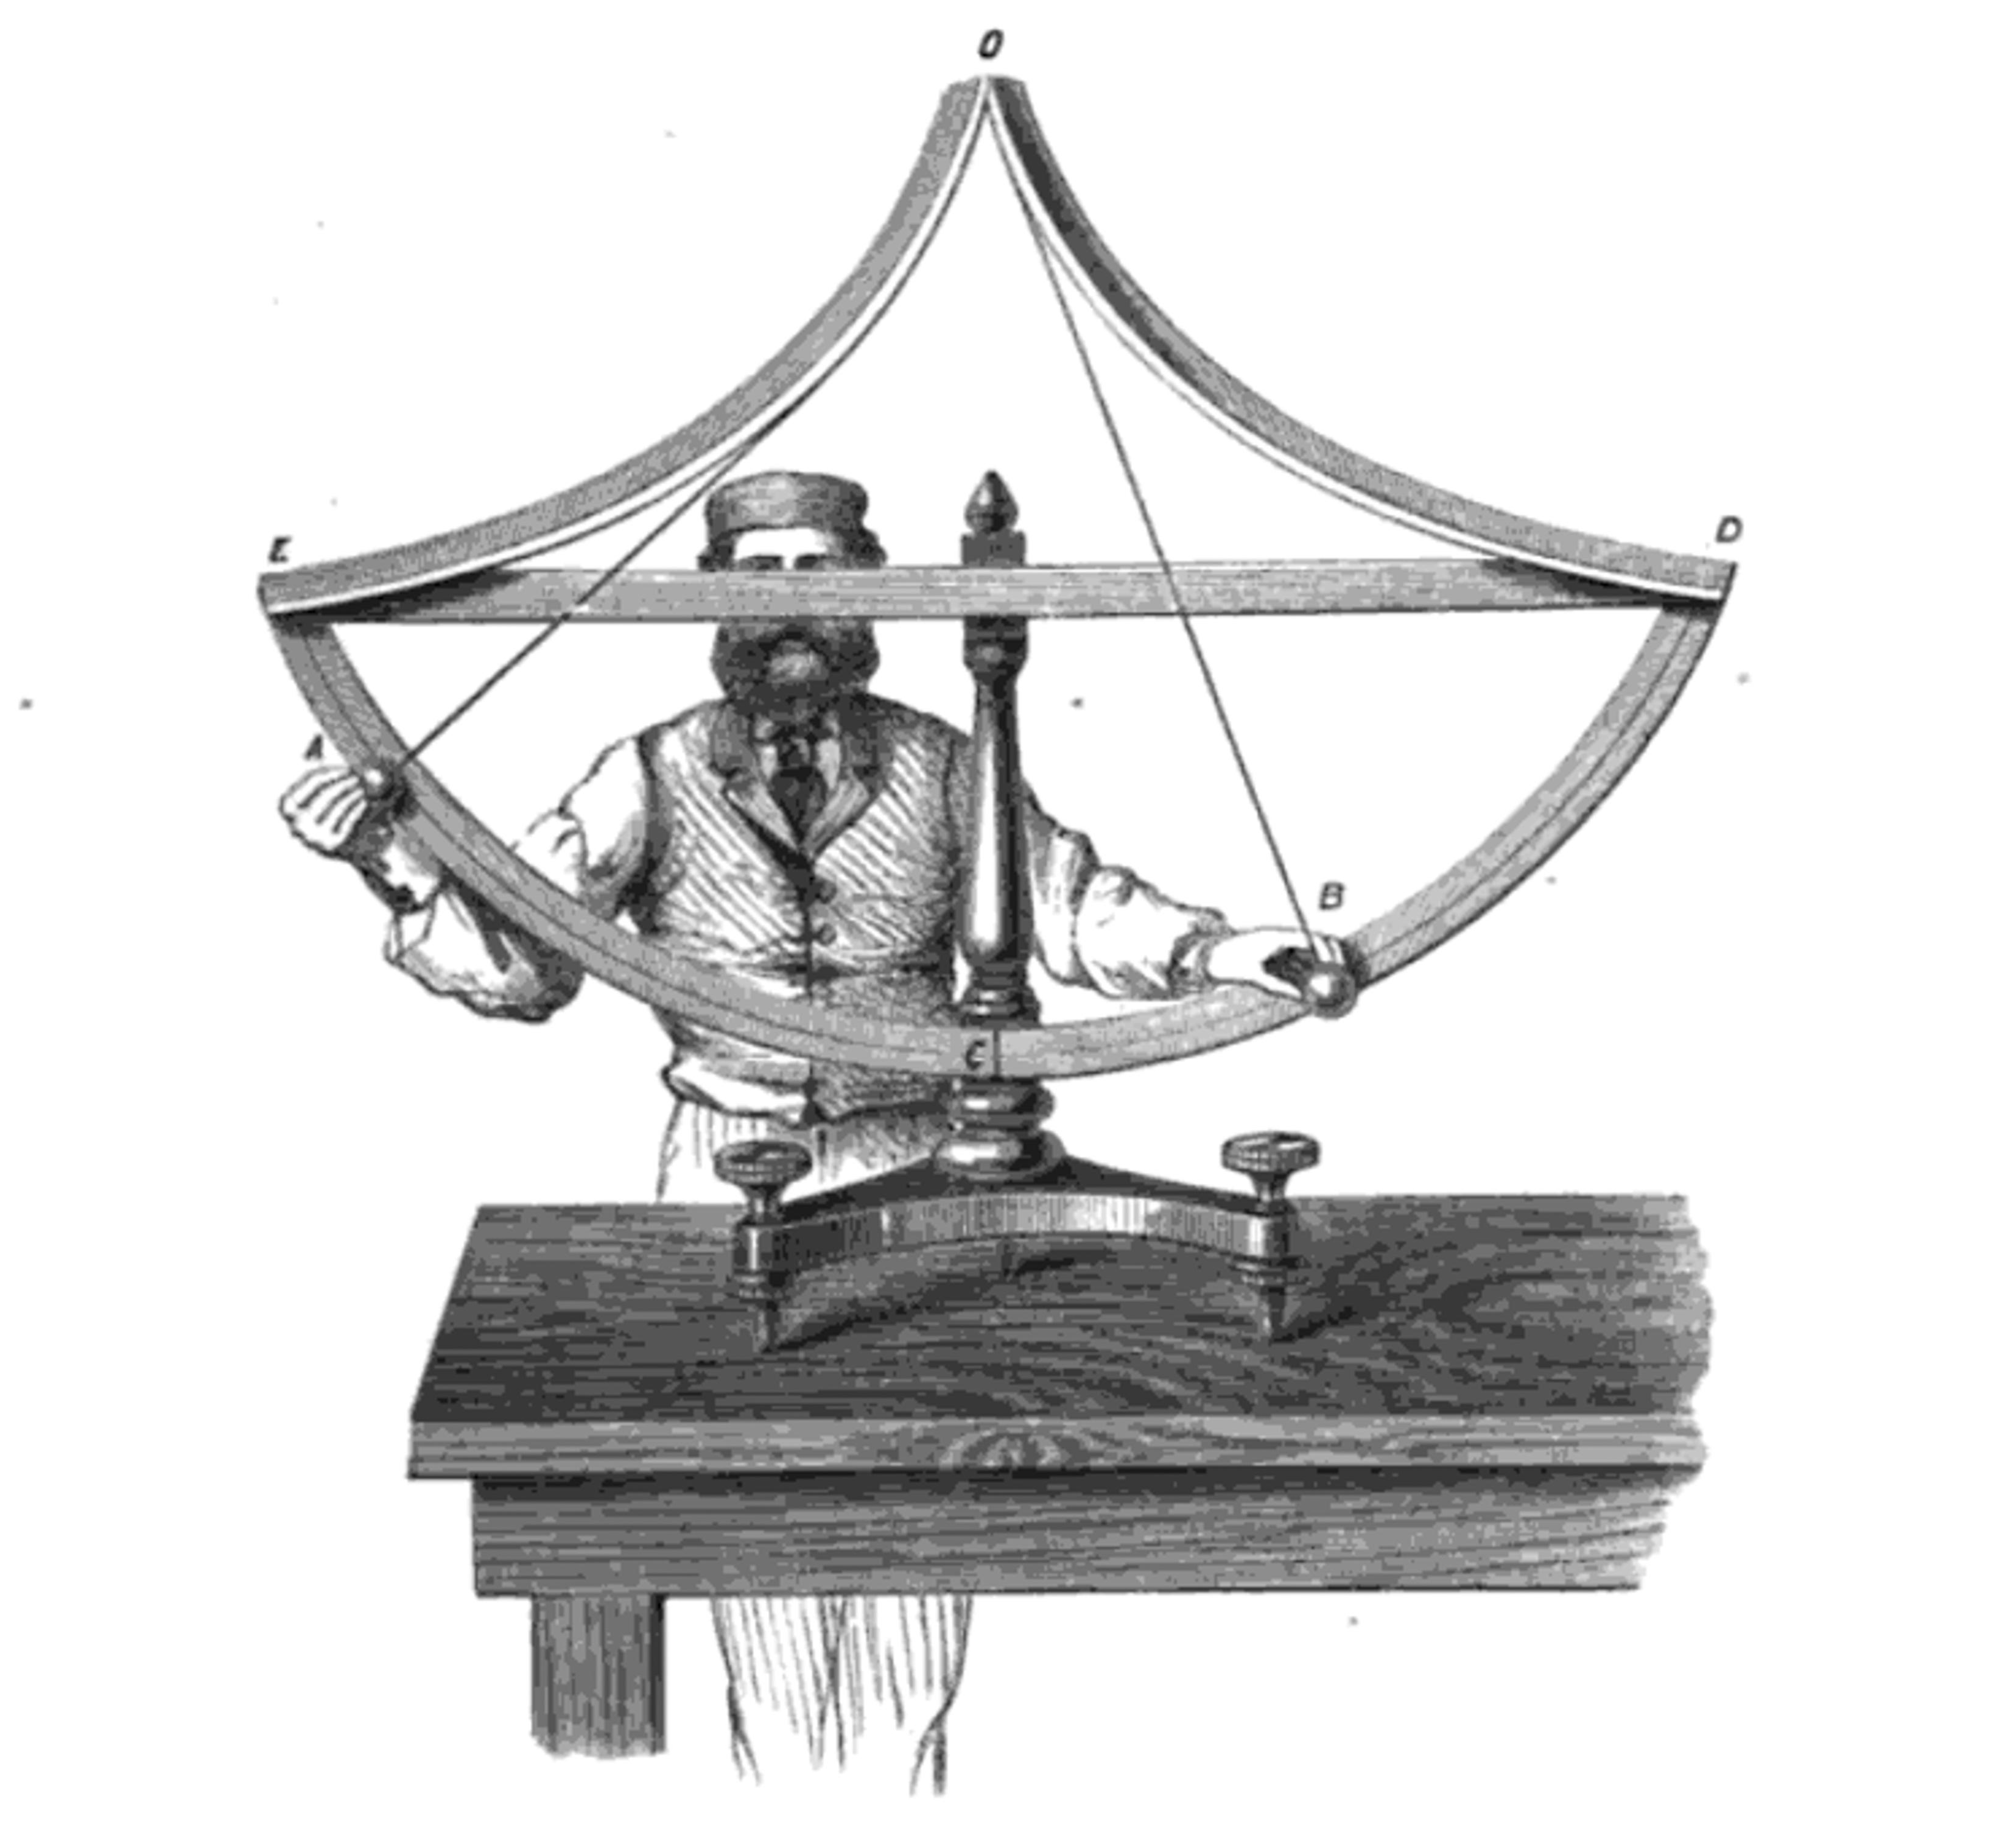
\includegraphics[width=0.5\textwidth]{Zykloidenpendel.jpg}}
\leftcaption[Brachistochrone aus dem Museo Galileo Florenz.]{Brachistochrone aus dem Museo Galileo Florenz. Gebaut von Francesco Spighi (Florenz, 2.\ H�lfte 18.~Jh.)\, \textcopyright Museo Galileo.} \label{abb:bew_Zykloid04}
\rightcaption[Konstruktion eines Zykloidenpendels.]{Konstruktion eines Zykloidenpendels.} \label{abb:bew_Zykloid05}
\end{minipage}
\end{figure}

Wir wissen also, dass die Brachistochrone eine Zykloide ist.
Nun untersuchen wir, wie die Bewegung auf derselben \bzw ihrer gespiegelten Kurve verl�uft.
Das \pot{} ist gegeben durch 
\begin{align}
	U = m\,g\,z = A\,\lk \cos\varphi - 1\rk \,.\label{eq:bew_Zykloid14}
\end{align}
Wir benutzen die Identit�t
\[ 1 - \cos\varphi = 2 \sin^2 \lk \frac{\varphi}{2} \rk \]
und erhalten mit $\varphi$ als generalisierter Koordinate die Lagrange-Funktion eines Teilchens, welches sich auf der Zykloidenbahn bewegt:
\begin{align}
    \mathcal{L} = \sin^2\frac{\varphi}{2}\,\lek \frac{m}{2} \lk 2A \rk^2 \dot{\varphi}^2 + m\,g\,\lk 2A \rk \rek \,.\label{eq:bew_Zykloid15}
\end{align}
Als Anfangs- \bzw Randbedingungen haben wir: $\varphi(0) = 0\,, \dot{\varphi}(0) = 0$ \bzw $0 < \varphi(x_\text{E}) < 2\pi$.
Durch die Substitution $q = \cos\frac{\varphi}{2}$ vereinfacht sich \eqref{eq:bew_Zykloid15} zu
\begin{align}
	\mathcal{L} = 8 m\, A^2\,\dot{q}^2 + 2m\,g\,A\, \lk 1 - q^2 \rk \,.\label{eq:bew_Zykloid16}
\end{align}
Die Lagrange-Gleichung \bzgl $q$ ergibt schlie�lich die Bewegungsgleichung eines Teilchens auf der Zykloide:
\begin{align}
	\ddot{q} = - \frac{g}{4A} q = {\omega_\text{zyk}}^2\,q \,.\label{eq:bew_Zykloid17}
\end{align}
Das ist aber die Bewegungsgleichung einer harmonischen Schwingung mit der \\
Kreisfrequenz $\omega_\text{zyk}$.
Im Gegensatz zum Pendel nach Gleichung \eqref{eq:bew_pendulum04} ist also die Bewegung auf der Zykloide exakt harmonisch, die Schwingungsfrequenz ist unabh�ngig von der Amplitude.
Damit ist die Zykloide eine Tautochrone.
Betrachtet man eine Zykloide, deren tiefster Punkt bei $(x_\text{T},\,z_\text{T})$ liegt, dann kommt ein Massepunkt an diesem Tiefpunkt immer zur gleichen Zeit an, ganz egal, von welcher H�he $z_\text{A}$ aus er startet.
Bereits Huygens erkannte dies und konstruierte eine Pendeluhr, die auf der Eigenschaft des Zykloidenpendels beruht.
Dies ist ein Pendel, bei dem der Faden zwischen zwei Zykloidenb�gen h�ngt und genau die L�nge des halben Zykloidenbogens hat (\figref{bew_Zykloid05}).
Dann beschreibt auch die Masse am Fadenende genau eine (gespiegelte) Zykloide.
Leider musste Huygens feststellen, dass die Gangungenauigkeit aufgrund der erh�hten Reibung an den Auflagefl�chen gr��er war als der Genauigkeitsgewinn durch die tautochrone Schwingung. \\


\subsubsection{Parametrische Oszillatoren -- Schaukel} \index{Oszillator!parametrischer}\label{kap:bew_pendulum_param}

Ein parametrischer Oszillator ist ein schwingendes System mit zeitabh�ngigen Parametern, durch die \zb Eigenfrequenz und D�mpfung ver�ndert werden k�nnen.
Dem Oszillator kann auf diese Weise Energie zugef�hrt werden, um die Amplitude der Schwingung zu vergr��ern.
Das am h�ufigsten zitierte Beispiel ist das Schwungholen bei einer Schaukel durch periodisches Heben und Senken des Schwerpunkts des schaukelnden K�rpers.
Ein solcher Oszillator mit rein parametrischer Anregung l�sst sich durch folgende homogene lineare Differentialgleichung beschreiben:
\begin{align}
		\ddot {x}+p_{1}(t){\dot {x}}+p_{2}(t) x=0 \,.	\label{eq:bew_schaukel01a}
\end{align}
Die zeitabh�ngigen Parameter $p_{1}$ und $p_{2}$ lassen sich zu einer zeitabh�ngigen Anregungsfunktion zusammenfassen, die man auch Pumpfunktion des Systems nennt.
Im Fall der Schaukel ist dies nat�rlich die eigene K�rperkraft, die ein Heben und Senken des K�rperschwerpunktes bewirkt.
Ein Merkmal einer rein parametrisch erzeugten Schwingung ist, dass sie ohne eine anf�ngliche Auslenkung aus der Ruhelage nicht entstehen kann, denn f�r die Anfangsbedingungen $(x,{\dot {x}})=(0,0)$ erh�lt man immer ${\ddot {x}}=0$.
Wir werden aber sehen, dass es schon bei infinitesimalen (unbeabsichtigten oder thermisch bedingten) Auslenkungen zu einer parametrischen Oszillation auch aus der Null-Lage kommen kann.
Die parametrische Anregung kann aber auch durch eine Zwangserregung erg�nzt werden, so dass die Differentialgleichung \eqref{eq:bew_schaukel01a} inhomogen wird.
Man spricht dann von einer kombinierten Zwangs- und Parametererregung:
\begin{align}
		{\ddot {x}}+p_{1}(t){\dot {x}}+p_{2}(t){x}=p_{3}(t) \,.	\label{eq:bew_schaukel01b}
\end{align}
Von besonderem praktischem Interesse \zb bei der Schaukel ist der Resonanzfall, bei dem die Parameter $p_{1}(t)$ und $p_{2}(t)$ mit doppelter Eigenfrequenz des Oszillators zeitlich variieren (\probref{bew_schaukelI}). 

\begin{figure}
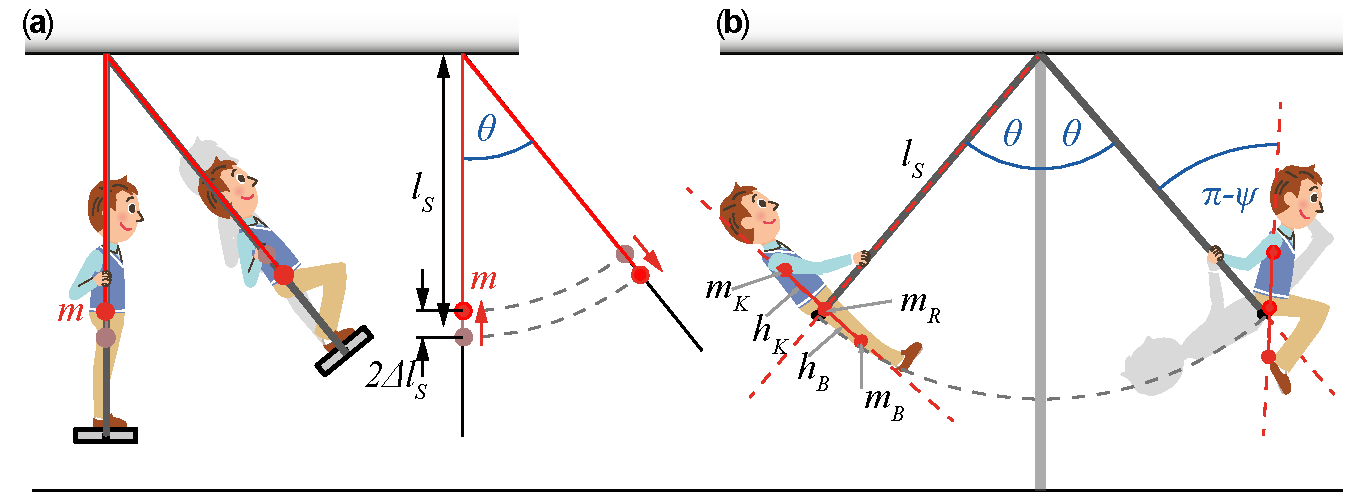
\includegraphics[width=\textwidth]{Schaukel01.pdf}
\caption[Modelle einer Schaukel.]{Modelle einer Schaukel. \fa Einfaches Massepunkt-Modell \fb Verbessertes Schaukelmodell mit sitzender Person als starren K�rper.}
\label{abb:bew_schaukel01}
\end{figure}

%\subparagraph{\textbf{Schaukelmodell a}}
Wir wollen zun�chst mit einem idealisierten Modell nach \figref{bew_schaukel01} a arbeiten und nur die Bewegung des Schwerpunktes entlang der Pendelaufh�ngung betrachten.
Bei Beginn des Schaukelns sei die Energie des Systems (\zb durch Ansto�en oder eine kleine Initialauslenkung) gegeben durch
        \begin{align}
            E_0 = m\,\frac{{v_0}^2}{2} = m\,g\,l_\text{S}\lk 1-\cos\theta_{\text{A}0}\rk\,. \label{eq:bew_schaukel01}
        \end{align}
Hierin ist $l_\text{S}$ die L�nge der Schaukel. Im Moment des Aufrichtens am Tiefpunkt verrichtet der Schaukelnde gegen die Schwer- und Zentrifugalkraft die Arbeit
        \begin{align}
            W_{\text{Unten}} = F\,\Delta l_\text{S} = \lk m\,g+\frac{m\,{v_0}^2}{l_\text{S}}\rk \,\Delta l_\text{S} \,, \label{eq:bew_schaukel02}
        \end{align}
wobei hierbei $F$ als ann�hernd konstant w�hrend der Bewegung angenommen wurde, was f�r ${\Delta l_\text{S}}/{l_\text{S}} \ll 1$ gut erf�llt ist. \\
Nach diesem \anf{Pumpen} im Durchgang durch den Tiefpunkt der Schaukel hat das System die Energie
        \begin{align}
            E_0' = E_0 + W_{\text{Unten}} = m\,g\,\Delta l_\text{S} +E_0\lk 1+ \frac{2\Delta l_\text{S}}{l_\text{S}}\rk \,.\label{eq:bew_schaukel03}
        \end{align}
Am Umkehrpunkt der Schaukel $\theta_\text{A}$ ist die Arbeit
    \begin{align}
        W_\text{Oben} = -m\,g\,\Delta l_\text{S}\,\cos\theta_{\text{A}} = -m\,g\,\Delta l_\text{S}+E_0'\,\frac{\Delta l_\text{S}}{l_\text{S}} \,, \label{eq:bew_schaukel04}
    \end{align}
und damit 
    \begin{align}
         E_0'' &= E_0' +  W_\text{Oben} = E_0 \lk 1+\frac{2\Delta l_\text{S}}{l_\text{S}}\rk + m\,g\,\Delta l_\text{S} - m\,g\,\Delta l_\text{S}\,\cos\theta_{\text{A}} \nonumber\\
        &= m\,g\,\Delta l_\text{S} \lk 1-\cos\theta_{\text{A}} \rk + E_0\lk 1+\frac{2\Delta l_\text{S} }{l_\text{S}}\rk = E_0'\,\frac{\Delta l_\text{S}}{l_\text{S}}+E_0\,\lk 1+\frac{2\Delta l_\text{S}}{l_\text{S}}\rk \\
        &=  m\, g\, \frac{\Delta l_\text{S}^2}{l_\text{S}} + E_0 \lk \frac{\Delta l_\text{S}}{l_\text{S}}+\frac{2\Delta l_\text{S}^2}{l_\text{S}^2}\rk+E_0\lk 1+\frac{2\Delta l_\text{S}}{l_\text{S}}\rk \approx E_0 \lk 1+\frac{3\Delta l_\text{S}}{l_\text{S}}\rk \,,
        \label{eq:bew_schaukel05}
    \end{align}
wobei wir wegen $\Delta l_\text{S} /l_\text{S} \ll 1$ quadratische Terme in $\Delta l_\text{S}$ vernachl�ssigen.
Nach einer vollen Periode haben wir zwei solcher Energie�nderungen $E_0''$, sodass nach $n$ Perioden 
        \begin{align}
            E_n =  E_0 \lk 1 + \frac{3\Delta l_\text{S}}{l_\text{S}} \rk^{2n} \,, \label{eq:bew_schaukel06}
        \end{align}
ist, wobei $n$ die Anzahl der Pendelperioden ist.
Die Beziehung f�r die Energie der Schaukel kann n�herungsweise geschrieben werden als 
        \begin{align}
            E_n =  E_0\, \mathrm{exp}\lk\frac{6n\,\Delta l_\text{S}}{l_\text{S}} \rk \,. \label{eq:bew_schaukel07}
        \end{align}
Es ist interessant zu bemerken, dass f�r dieses einfache System der relative Energiezuwachs $E_n/E_0$ nicht von der Masse abh�ngig ist (wohl aber von $\Delta l_\text{S}$).\\
Mit der Schwingungsperiode eines linearen Pendels mit
$T_\text{P}=2\pi\sqrt{l_\text{S}/g}$, $t=n\,T_\text{P}$ und $\Delta l_\text{S}/l_\text{S} = 2\Delta T_\text{P}/T_\text{P} = 2\Delta f/f = 2\,\Delta f\,T_\text{P}$
k�nnen wir \eqref{eq:bew_schaukel07} schreiben als
        \begin{align}
            E\lk t\rk = E_0\, \text{exp}\lk 12\:\Delta f\,t\rk \,. \label{eq:bew_schaukel08}
        \end{align}
Dies ist eine interessante Formel, die bis auf den Faktor 12 auch f�r sogenannte \emph{parametrische Oszillatoren und Verst�rker} \index{Verst�rker!parametrischer} G�ltigkeit hat.
Offensichtlich zeigt \eqref{eq:bew_schaukel08}, dass es f�r $E_0 = E\lk 0 \rk = 0$ keine parametische Verst�rkung geben kann.
Wenn man allerdings \zb durch die Luftbewegung eine Initialgeschwindigkeit von $v_0=\SI{1}{\cm\per\second}$ und die Parameter $m=\SI{50}{\kilogram}$, $l_\text{S}=\SI{3}{\metre}$ und $\Delta l_\text{S}=\SI{15}{\cm}$ annimmt, dann erh�lt man $E_0 = \SI{25e-4}{}\mathrm{Nm} $ und $f=\SI{0.29}{\per\second}$ und damit $E(t) = E_0\,\mathrm{exp}\lk{+12\,\Delta f\,t}\rk\approx E_0 \, \mathrm{exp}\lk{0.086\,t}\rk$.
Man erkennt, dass auch in diesem Fall die Energie schnell zunehmen kann und eine Auslenkung von $\theta_\text{A}=45\degree$ (wobei die harmonische N�herung, die wir hier benutzt haben, schon l�ngst versagt) nach ca.\ $t \approx \SI{4.6}{\second}$ erreicht wird. \\
Zur Berechnung der Zeitentwicklung k�nnte man dieses einfache Modell der Schaukel mit folgender DGL mathematisch beschreiben, wobei wir einen quadratischen Reibungsterm mitgenommen haben:
    \begin{align}
		\begin{split}
       &\ddot{\theta} + \eta\dot{\theta}^2+ \frac{l_\text{S}\lk t\rk}{g}\,\sin\theta = 0 ~~~ \text{mit}~~~ l_\text{S}\lk t\rk = l_\text{S}-\Delta l_\text{S} \,\cos\lk \omega_\text{A}\,t\rk  \,,\\
       &\ddot{\theta} + \eta\dot{\theta}^2+ \omega\lk t \rk\,\sin\theta = 0 ~~~ \text{mit}~~~ \omega\lk t\rk = \omega_0^2 - {\Delta\omega}^2 \,\cos\lk \omega_\text{A} \, t + \varphi_\text{A}\rk \,. 
		\end{split} \label{eq:bew_schaukel08a}
    \end{align}
    Wir l�sen diese numerisch im \mscr{} \mlbewref{Schaukel01.m} und zeigen das Ergebnis f�r verschiedene Parameter in \figref{bew_schaukel02}.

\begin{figure}
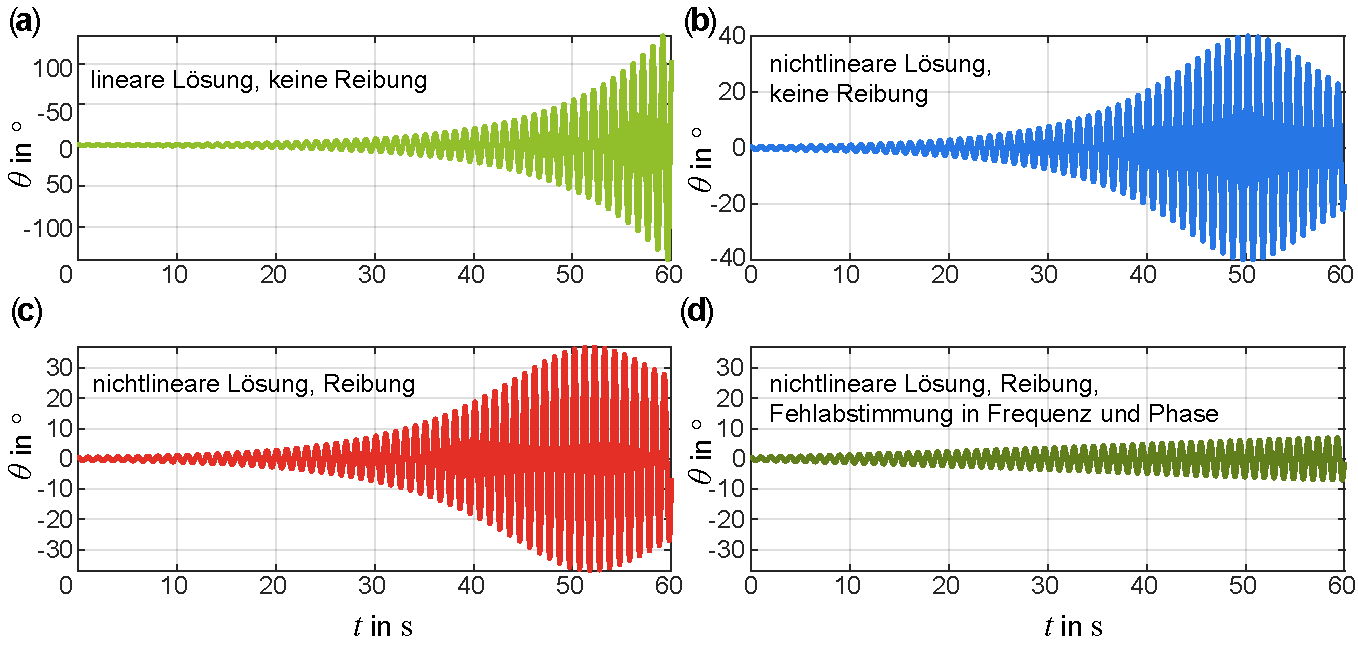
\includegraphics[width=\textwidth]{Schaukel04.pdf}
\caption[L�sung der Bewegungsgleichung eines parametrischen Oszillators.]{%
L�sung der Bewegungsgleichung f�r das Modell einer Schaukel als Beispiel eines parametrischen Oszillators.
Die Parameter aus \eqref{eq:bew_schaukel08a} sind: $\omega_0 = 2\pi\SI{}\second$, $\Delta\omega = 0.3\,\omega_0$, $\omega_\text{A} = 2\,\omega_0$ und $\varphi_\text{A} = 0$  (keine Fehlabstimmung), $\omega_\text{A} = 2.02\,\omega_0$ und $\varphi_\text{A} = \pi/4$  (Fehlabstimmung), $\eta = \SI{0.01}{\per\second\squared}$ (Reibung).
In der linearen N�herung \fa wurde die $\sin(\theta)$-Funktion in \eqref{eq:bew_schaukel08a} durch $\theta$ approximiert.
Man erkennt das exponentielle Aufschaukeln im Fall ohne Reibung, in der L�sung f�r den nichtlinearen Fall \fb -- \fd erzeugt die entstehende Fehlabstimmung der parametrischen Anregung automatisch eine Begrenzung und ein \anf{Abschaukeln}, man muss beim Schaukeln also die parametrische Frequenz der momentanen Eigenfrequenz anpassen, um Anregung zu erhalten.
\fc Ebenso entsteht eine zus�tzliche Begrenzung durch die Reibung. \fd Bei einer Fehlabstimmung in Frequenz und Phase erfolgt das Aufschaukeln deutlich langsamer.} \label{abb:bew_schaukel02}
\end{figure}

Wir wollten unsere Modellrechnung noch auf dem Spielplatz testen.
Bei der Beobachtung der schaukelnden Kinder stellen wir jedoch fest, dass anders als im Modell beschrieben, die meisten Kinder im Sitzen schaukeln und dabei eine Vor- und R�ckw�rtsbewegung des Oberk�rpers und der Beine ausf�hren, w�hrend der Schwerpunkt des K�rpers relativ zum Schaukelsitz mehr oder weniger in Ruhe bleibt.
Wir m�ssen also diese Bewegung in einem verbesserten Modell des schaukelnden K�rpers gem�� \figref{bew_schaukel01}b abbilden, was den Begriff des Tr�gheitsmoments\index{Tr�gheitsmoment} voraussetzt, den wir erst bei der Behandlung des starren K�rpers in \kap{bew_starrer_koerper} kennen lernen werden.
Wir werden dort in \kap{bew_pendulum_schaukel} dann auch ein verbessertes Modell der Schaukel angeben und durchrechnen.

\subsubsection{Das Foucault-Pendel} \index{Pendel!Foucault-}\index{Foucault-Pendel}\label{kap:bew_pendulum_foucault}

Bisher haben wir stillschweigend bei der Betrachtung der Pendelbewegung angenommen,
dass diese in einem Inertialsystem stattfindet. 
Wir wollen diese Annahme jetzt fallen lassen und fragen uns, wie die Pendelbewegung in einem mitrotierendem Koordinatensystem berechnet werden kann.
Wir betrachten dazu ein \emph{Foucault-Pendel}.
Diese Pendelanordnung mit gro�er Pendell�nge und -masse, die erstmalig 1851 von L�on Foucault%
\footnote{Jean Bernard L�on Foucault\indexp{Foucault, Jean Bernard L�on} (1819--1868) war ein franz�sischer Physiker und Astronom,
der bedeutende Beitr�ge auf dem Gebiet der Optik lieferte, aber auch im Design mechanischer Instrumente t�tig war.}
vorgestellt wurde, erm�glicht ohne zus�tzliche astronomische Beobachtungen den Nachweis der Erd\-rotation. 
Das Pendel wird dazu m�glichst reibungslos aufgeh�ngt,
wobei die Wirkung der Luftreibung im Verh�ltnis zur Gravitations- und Coriolis-Kraft
aufgrund der gro�en Masse vernachl�ssigt werden kann.
Das Prinzip ist recht einfach zu verstehen, denn die wesentliche Auswirkung der Rotation der Erde besteht darin, dass diese sich unter der im Inertialsystem feststehenden Schwingungsebene des Pendels wegdreht.
Am Nord- oder S�dpol ist dies am leichtesten einzusehen, weil der Aufh�ngepunkt des Pendels dort trotz der Erddrehung in Ruhe bleibt.
Daher w�rde die Erde sich an einem Tag\footnote{Genau gesprochen: einem Sternentag $=\SI{86164}{\s}$ (siehe Himmelsmechanik im Band II, Kapitel 3).} genau einmal voll unter dem Pendel hinwegdrehen.

\begin{figure}
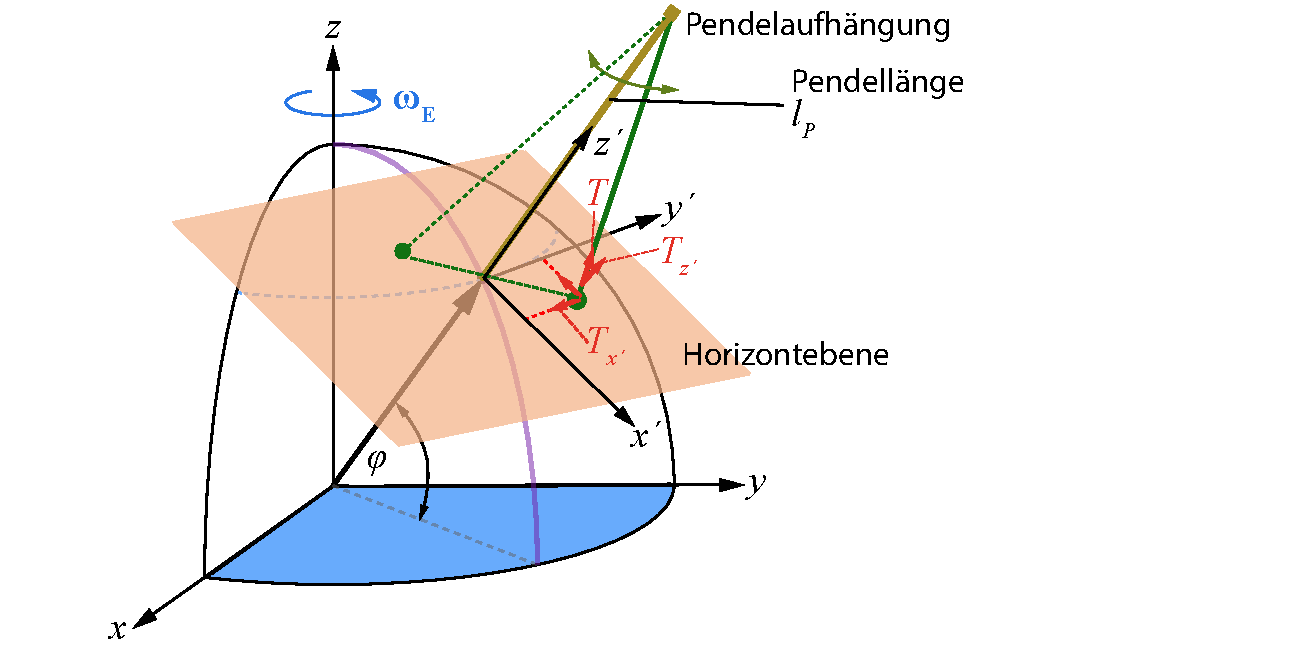
\includegraphics[width=\textwidth]{FoucaultPendel01.pdf}
\caption[Mitbewegtes Koordinatensystem f�r Foucault-Pendel.] {Mitbewegtes Koordinatensystem auf der Erdoberfl�che f�r die Betrachtung des Foucault-Pendels. Die Pendell�nge ist $l_\text{P}$ und die $T_{x'}', T_{y'}', T_{z'}'$ sind die Komponenten der Spannungskr�fte im Pendelarm im mitbewegten Koordinatensystem gemessen.}
\label{abb:bew_Foucault_01}
\end{figure}

In \kapitel{bew_Coriolis-Kraft} haben wir gesehen, wie die Scheinkr�fte auf bewegte K�rper f�r einen Beobachter im mitbewegten KOS wirken.
Bei einer Behandlung der Bewegung eines Foucault-Pendels im mitbewegten \KOS der Erde m�ssen diese Kr�fte nat�rlich im Rahmen der Newtonsche Mechanik mit ber�cksichtigt werden.
Wir starten dazu mit \eqref{eq:bew_BGL_Erdrotation} und erinnern uns,
dass die $x'$-Achse nach S�den und die $y'$-Achse nach Osten ausgerichtet ist (\figref{bew_Rot_Erde1}).
Unser Massepunkt soll jetzt an einem langen Faden der L�nge $l_\text{P}$ senkrecht auf der $x'$-$y'$-Ebene (also in $z'$-Richtung) aufgeh�ngt sein (\figref{bew_Foucault_01}).
Dann lautet die entsprechend aus \eqref{eq:bew_BGL_Erdrotation_Ko} abgeleitete Bewegungsgleichung f�r das Pendel
    \begin{align}
        \begin{pmatrix}
        \ddot{x}' \\
        \ddot{y}' \\
        \ddot{z}'
        \end{pmatrix}
        = -2\,\omega_\text{E}
        \begin{pmatrix}
        -\dot{y}'\sin\varphi \\
        \dot{x}'\sin\varphi + \dot{z}'\cos\varphi\\
        -\dot{y}'\cos\varphi + \frac{g}{2\omega_\text{E}}
        \end{pmatrix}
        + \frac{1}{m}
        \begin{pmatrix}
        T_{x'}' \\
        T_{y'}' \\
        T_{z'}'
        \end{pmatrix} \,,\label{eq:bew_BGL_Foucault}
    \end{align}
wobei wir vereinfachend die Zentrifugalkraft in eine effektive Erdanziehungskraft (Gravitation) eingeschlossen haben, also $F_\text{G} = m g$; der Winkel 
$\varphi$ ist wieder die geographische Breite. 
Die $T_\text{i'}'$ sind die Fadenspannungen in den drei Koordinaten, die die Masse an der Aufh�ngung halten (\figref{bew_Foucault_01}).

Wir wollen uns nun im wesentlichen die Projektion eines (relativ langen) Pendels auf die $x'$-$y'$-Ebene anschauen, sodass wir $\dot{z}'=0$ setzen k�nnen.
Aus \figref{bew_Foucault_01} sehen wir, dass f�r kleine Auslenkungen ${z'}/{l_\text{P}} \approx 1$ gilt und somit auch:
		\begin{align*}
				T_\text{z'}' &= -\,m\,g\,\frac{z'}{l_\text{P}} \approx m\,g \,, \\
				T_\text{x'}' &= -\,m\,g\,\frac{x'}{l_\text{P}}  \,, \\
				T_\text{y'}' &= -\,m\,g\,\frac{y'}{l_\text{P}} \,.
		\end{align*}
Zusammen mit der N�herung $\dot{z}'=0$ erhalten wir
		\begin{align}
				\begin{pmatrix}
				\ddot{x}' \\
				\ddot{y}'
				\end{pmatrix}
				= 
				\begin{pmatrix}
				+2\omega_\text{E}\,\dot{y}'\,\sin\varphi - \frac{g}{l_\text{P}}x'\\
				-2\omega_\text{E}\,\dot{x}'\,\sin\varphi - \frac{g}{l_\text{P}}y'
				\end{pmatrix} \,.
				\label{eq:bew_Foucault_02}
		\end{align}
Wir setzen ${\omega_0}^2= \frac{g}{l_\text{P}}$ als das Quadrat der Schwingungsfrequenz des Pendels der L�nge $l_\text{P}$ und k�nnen mit $Q = x'+i\,y' $ vorteilhaft die beiden Gleichungen aus \eqref{eq:bew_Foucault_02} zu einer komplexen Gleichung kombinieren:
		\begin{align}
				\ddot{Q} + 2 \mathrm{i} \,\omega_\text{F}\,\dot{Q}+{\omega_0}^2\,Q = 0  \qquad \text{mit} \qquad \omega_\text{F} = \omega_\text{E} \sin\!\varphi\,. \label{eq:bew_Foucault_03}
		\end{align}
Die Struktur dieser Gleichung entspricht der eines ged�mpften Oszillators \eqref{eq:bew_pendulum02}.
Deren L�sung war durch \eqref{eq:bew_pendulum04} gegeben, was hier nun bedeutet:
	\begin{align*}
		Q \lk t \rk &= x' +\im\,y'\\
		&= Q_0 e^{-\im\,\omega_\text{F}\,t}e^{\pm \im\,\hat{\omega}_0\,t} \qquad \text{mit} \qquad \hat{\omega}_0 = \sqrt{{\omega_0}^2+{\omega_\text{F}}^2}  \\
		&= Q_{01}\,e^{-\im\,\omega_\text{F}\,t}e^{\im\,\hat{\omega}_0\,t} + Q_{02}\,e^{-\im\,\omega_\text{F}\,t}e^{-\im\,\hat{\omega}_0\,t} \,.
	\end{align*}
Ganz allgemein k�nnen wir $Q_{01} = Q_{02} = \frac{Q_0}{2}$ setzen und erhalten
	\[Q \lk t \rk = Q_0\,e^{-\im\,\omega_\text{F}\,t}\cos\hat{\omega}_0 t = \lk x_0'+\im\,y_0'\rk \cos\hat{\omega}_0 t\,\lek\cos\omega_\text{F} t - \im\,\sin\omega_\text{F} t\rek \,,\]
sodass f�r $x(t)',\,y(t)'$ gilt:
    \begin{align}
        x'\lk t \rk &= + x_0'\cos\hat{\omega}_0 t\,\cos\omega_\text{F} t + y_0'\cos\hat{\omega}_0 t\,\sin\omega_\text{F} t \,,\notag\\
        y'\lk t \rk &= -x_0'\cos\hat{\omega}_0 t\,\sin\omega_\text{F} t + y_0'\cos\hat{\omega}_0 t\,\cos\omega_\text{F} t \,, \notag\\
    %\end{align*}
    \intertext{\bzw in Matrixschreibweise}
    %\begin{align}
        \begin{pmatrix}
            x'\lk t \rk \\
            y'\lk t \rk
        \end{pmatrix}
        &=
        \begin{pmatrix}
            +\cos\omega_\text{F}t & \, +\sin\omega_\text{F}t \\
            -\sin\omega_\text{F}t & \, +\cos\omega_\text{F}t
        \end{pmatrix}
        \begin{pmatrix}
            x_\text{P}'\lk t \rk \\
            y_\text{P}'\lk t \rk
        \end{pmatrix} \,,
        \label{eq:bew_Foucault_05}
    \end{align}
worin
		\begin{align*}
				x_\text{P}'\lk t \rk &= x_0'\cos\hat{\omega}_0 t + y_0' \cos\hat{\omega}_0 t = \lk x_0' + y_0' \rk \cos\hat{\omega}_0 t \quad \text{und} \\
				y_\text{P}'\lk t \rk &= \lk y_0' -x_0' \rk \cos\hat{\omega}_0 t
		\end{align*}
die Eigenl�sung des (harmonischen) Pendels ist. 
Die Matrix in \eqref{eq:bew_Foucault_05} ist offensichtlich eine Rotationsmatrix (siehe \kap{bew_rotating_systems}).
Damit beschreibt \eqref{eq:bew_Foucault_05} die zeitabh�ngige Drehung der Pendelebene, die durch die Vektoren $x_0'\lk t \rk \vecpeX + y_0'\lk t \rk \vecpeY ~\text{und} ~\vecpeZ$ aufgespannt wird.
Die Drehfrequenz $\omega_\text{F}$ h�ngt �ber $\omega_\text{F} = \omega_\text{E} \sin\varphi$ von der geographischen Breite ab,
sie ist am Pol maximal\footnote{Am Pol ist das Bild der Drehung der Pendelebene auch sehr anschaulich. F�r einen Beobachter im Inertialsystem steht die Ebene fest, die Beobachtungsebene dreht sich quasi unter der Aufh�ngung mit $\omega_\text{E}$ weg.} und verschwindet am �quator.
F�r das ber�hmte Foucault-Pendel im Deutschen Museum M�nchen ergibt sich
f�r das $\SI{60}{\metre}$ lange Seil und die geographische Breite von $\varphi = \SI{48.1}\degree$
eine Foucault-Rotationsperiode von 
\[T_\text{F} = \frac{2\pi}{\omega_\text{F}}\approx \SI{32}{\hour}\,\SI{8}{\minute}\]
bei einer Pendelperiode von $T_\text{P} = 2\pi\sqrt{\frac{l_\text{P}}{g}} \approx \SI{15.5}{\second}$.
Nach etwa $\SI{30}{\minute}$ hat sich die Pendel\-ebene also um etwa $\SI{5.6}\degree$ gedreht. \\
F�r ein deutlich schneller rotierendes KOS haben wir zur Veranschaulichung des Foucaultpendels in \figref{bew_Foucault_02} die Projektion des Pendels auf die $x$-$y$-Ebene dargestellt (siehe auch \mscr{} \mlbewref{FoucaultPendel.m}).

\begin{figure}
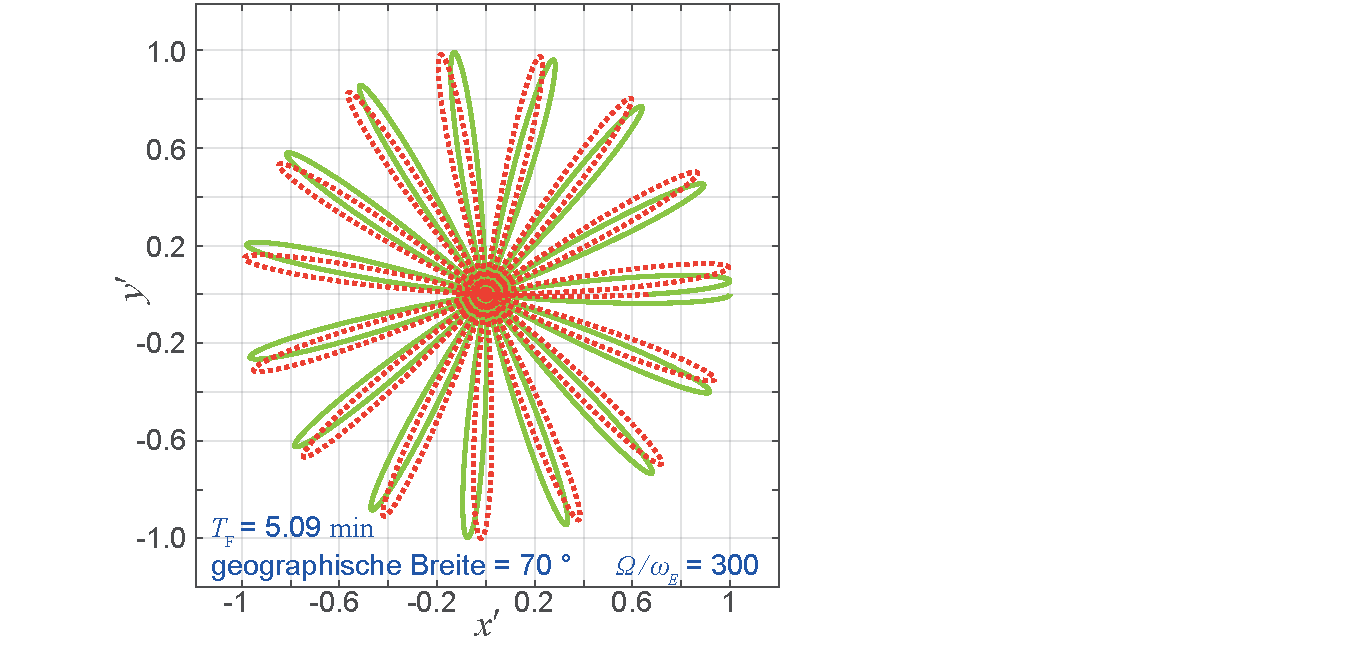
\includegraphics[width=\textwidth]{FoucaultPendel02.pdf}
\caption[Bahnkurve eines Foucault-Pendels bei "`schnellerer"' Erdrotation.] {Bahnkurve eines Foucault-Pendels bei einer angenommenen 300-fach schnelleren Erdrotation. Die Pendell�nge ist $\SI{100}{\metre}$. Dargestellt sind zwei Pr�zessionsperioden des Pendels. Man erkennt, dass die Rosettenbahn nicht ganz geschlossen ist, da $\omega_\text{F}$ kein ganzzahliges Vielfaches von $\omega_\text{E}$ ist.} 
\label{abb:bew_Foucault_02}
\end{figure}

\medskip

Zum Schluss wollen wir noch die Bewegungsgleichung des Foucault-Pendels �ber die Lagrange-Funktion herleiten.
Wir schreiben zun�chst die Lagrange-Funktion $\mathcal{L}$ f�r das Pendel im Inertialsystem auf:
\begin{align*}
		\mathcal{L} &= T-U =\frac{m}{2}\lek \dot{x}^2 + \dot{y}^2 + \dot{z}^2 \rek -U \lk x,y,z\rk\,.
\end{align*}
Aus der allgemeinen Transformation von KOS nach \eqref{eq:bew_Rot_System1} folgt insbesondere f�r ein rotierendes System mit $\vec{v} = \vec{v}' + \vec{\omega}' \times \vec{r}'$, dass
\begin{align*}
\vec{\omega}' = \omega_\text{E} 
	\begin{pmatrix}
		-\cos\varphi\\
		0 \\
		\sin\varphi
	\end{pmatrix}~. 
\end{align*}	
Damit ergibt sich die Bewegungsgleichung des Pendels zu
		\begin{align}
				\begin{pmatrix}
					\dot{x}\\
					\dot{y} \\
					\dot{z}
				\end{pmatrix}  
				&=
				\begin{pmatrix}
					\dot{x}'\\
					\dot{y}' \\
					\dot{z}'
				\end{pmatrix} 
				+s
				\begin{pmatrix}
					-\omega_\text{E}'\,y' \sin\varphi\\
					\omega_\text{E}'\,x' \sin\varphi + \omega_\text{E}'\,z' \cos\varphi \\
					-\omega_\text{E}'\,y' \cos\varphi
				\end{pmatrix} \,. 
				\label{eq:bew_Foucault_06}
		\end{align}
Bei Vernachl�ssigung von $\dot{z}', z'$ und $\omega'^2$ wird daraus jetzt in Koordinaten des rotierenden Systems
    \begin{align*}
      T & = \frac{m}{2} \lek \dot{x}'^2 + \dot{y}'^2 + 2 \omega_\text{E} \sin\varphi \lk x'\,\dot{y}'-\dot{x}'\,y'\rk\rek \,,\\
      \text{und} ~~~U &= m\,g\,\Delta z = m\,g\,\Delta z'= m\,g \lk l_\text{P}-l_\text{P}\cos\theta\rk = m\,g\,l_\text{P}\lk 1-\sqrt{1-\sin^2\theta} \rk \,,\\
      &\overset{\sin\theta \ll 1}{=} m\,g\,l_\text{P}\, \frac{1}{2}\sin^2\theta = \frac{m\,g\,l_\text{P}}{2}\lk\frac{x'^2+y'^2}{l_\text{P}{}^2}\rk \,, \\
      \text{mit} ~~ x'&= l_\text{P} \sin\theta\cos\phi \,,~~  y'= l_\text{P} \sin\theta\sin\phi \,.
    \end{align*}
Somit erhalten wir f�r die Lagrange-Funktion in Koordinaten des mitbewegten Systems
    \begin{align}
                    \mathcal{L} = \frac{m}{2} \lek \dot{x}'^2 + \dot{y}'^2 + 2\omega_\text{E}\sin\varphi \lk x'\,\dot{y}' - \dot{x}'\,y'\rk \rek - \frac{m\,g}{2\,l_\text{P}}\lk x'^2 + y'^2 \rk \,. \label{eq:bew_Foucault_07}
    \end{align}
�ber die Lagrange-Gleichungen ergeben sich sofort die Bewegungsgleichungen \eqref{eq:bew_Foucault_02}, ohne dass man weitere geometrische �berlegungen zu den Zwangskr�ften anstellen muss.
Man erkennt auch hier den Vorteil des Lagrange-Formalismus (Lagrange-Gleichungen zweiter Art).
In Zusatzaufgabe \ref{prob:bew_Zusatz_Foucault} werden die Bewegungsgleichungen des Foucault-Pendels exakt gel�st
und die kleinen Abweichungen von den in diesem Kapitel angestellten N�herungsl�sungen auf Basis der Newtonschen Mechanik diskutiert.


\subsubsection{Gekoppelte und komplexe Pendel} \index{Pendel!gekoppelte} \label{kap:bew_pendulum_coupled}

Wir wollen uns nun interessanten Beispielen f�r \emph{gekoppelte} schwingende Systeme aus Federn und Pendeln zuwenden.
Wir betrachten dabei zun�chst wieder geringe Auslenkungen, um ein Verfahren kennenzulernen,
das auch bei einer gro�en Zahl gekoppelter Elemente im schwingenden System gut anwendbar ist
und zugleich eine sch�ne Anwendung der linearen Algebra darstellt.
Anschlie�end betrachten wir zwei Beispiele: das Stangenpendel und das Doppelpendel.
Die Zwangsbedingungen des Doppelpendels hatten wir bereits in 
\probref{bew_Zwangsbedingungen} hergeleitet (siehe auch \figref{bew_Doppelpendel01}).\\

\subparagraph{Linearisierung gekoppelter Systeme bei geringen Auslenkungen}

Wir betrachten ein gekoppeltes schwingendes System mit $N$ Massepunkten und $Z_\text{B}$ Zwangsbedingungen.
Befindet sich dieses System nahe der Gleichgewichtslage, so lassen sich die Bewegungsgleichungen mit den verbleibenden $F = 3N-Z_\text{B}$ Freiheitsgraden entkoppeln, indem sogenannte Normalkoordinaten eingef�hrt werden.
Man erh�lt dann $F$ einfache entkoppelte Schwingungsgleichungen f�r jede dieser Koordinaten.
%Wir wollen das im Folgenden zeigen.
F�r ein solches System nahe der Gleichgewichtslage k�nnen wir dazu die Beziehungen
\eqref{eq:bew_Schwingung_b} und \eqref{eq:bew_Schwingung_a} f�r die kinetische Energie $T$ und die potentielle Energie $U$ verwenden.
Mit den generalisierten Koordinaten $q_i$ k�nnen wir durch
\begin{equation}
	\zeta_i = q_i - q_{i,0} \label{eq:bew_Kopplg01}
\end{equation} 
neue Koordinaten als Verschiebung von der Gleichgewichtslage (Auslenkung) einf�hren.
Dabei gilt $\dot{\zeta}_i = \dot{q}_i$.\footnote{Man macht sich das leicht klar, indem man in Gleichung 
\eqref{eq:bew_Schwingung_b} die Taylor-Entwicklung ausf�hrt.}
Wir schreiben
\begin{align}
	T &= \frac{1}{2}\sum_{i,j=1}^{F} \underbrace{\sum_{k=1}^{N} \lk m_k \frac{\partial x_k}{\partial q_i} \cdot \frac{\partial x_k}{\partial q_j} \rk \bigg|_{q_0}}_{T_{ij}} \dot{q}_i \dot{q}_j 
	= \frac{1}{2} \sum_{i,j=1}^{F} T_{ij} \dot{\zeta}_i \dot{\zeta}_j ~~ \text{und} \nonumber \\
	U &= \frac{1}{2} \sum_{i,j=1}^{F} \frac{\partial^2 U}{\partial q_i \partial q_j} (q_i - q_{0,i})(q_j - q_{0,j}) \nonumber \\
	&= \frac{1}{2} \sum_{i,j=1}^{F} \frac{\partial^2 U}{\underbrace{\partial \zeta_i \partial \zeta_j}_{U_{ij}}} \zeta_i \zeta_j = \frac{1}{2} \sum_{i,j=1}^{F} U_{ij} \zeta_i \zeta_j \label{eq:bew_Kopplg02} ~.
\end{align}
Die Lagrange-Funktion f�r das Gesamtsystem ist dann
\begin{align}
	\mathcal{L} &= T - U = \frac{1}{2} \sum_{i,j=1}^{F} T_{ij} \dot{\zeta_i} \dot{\zeta_j} - \frac{1}{2} \sum_{i,j=1}^F U_{ij} \zeta_i \zeta_j \,.\label{eq:bew_Kopplg03}
\end{align}
Daraus k�nnen wir die Lagrange-Gleichungen in einer einfachen Matrixdarstellung\footnote{Im Folgenden werden Grundkenntnisse der linearen Algebra wie Diagonalisierung, Eigenwertbestimmung, charakteristische Gleichung \usw vorausgesetzt. Wir empfehlen dem Leser zur Wiederholung die \onlineZ{}~ \bzw die Referenzen \cite{Arens2008, Riley2006, Fischer2018, Bartelmann2015}.} ableiten:
\begin{equation}
	\mathbb{T} \ddot{\vec{\zeta}} + \mathbb{U} \vec{\zeta} = 0 \qquad \text{mit} \qquad 
	\vec{\zeta} =
	\begin{pmatrix}
		 \zeta_1 \\ \zeta_2\\ \vdots \\ \zeta_F
	\end{pmatrix}\,,	\label{eq:bew_Kopplg04}
\end{equation}
worin die Matrizen $\mathbb{T}$ und $\mathbb{U}$ durch die $T_{ij}$ bzw. $U_{ij}$ bestimmt sind.\footnote{Es ist eine instruktive �bung, die Herleitung von \eqref{eq:bew_Kopplg04} aus \eqref{eq:bew_Kopplg03} zu zeigen.
Dazu m�ssen die Matrizen symmetrisch sein.
Dies ist durch die Definitionen \eqref{eq:bew_Kopplg01} und \eqref{eq:bew_Kopplg02} automatisch erf�llt.} Wir haben mit \eqref{eq:bew_Kopplg04} aber immer noch ein verkoppeltes System, da die Matrizen ja Nebendiagonalelemente haben, die genau die Kopplungen beschreiben.
Wir m�ssen also durch Einf�hrung neuer Koordinaten $\vec{\xi_i}$ (\dh eine Koordinatentransformation $\vec{\zeta}\rightarrow\vec{\xi}$) versuchen, das Problem zu diagonalisieren\footnote{Das Ziel besteht also darin, durch die Koordinatentransformation $\zeta \rightarrow \xi$ die Matrizen $\mathbb{T}$ und $\mathbb{U}$ gleichzeitig zu diagonalisieren.
Man kann zeigen, dass dies m�glich ist, da beide Matrizen symmetrisch sind \cite{Bartelmann2015, Riley2006}.} und die Lagrange-Funktion damit in die Form
\begin{equation}
	\mathcal{L} = \frac{1}{2} \sum_{i=1}^F {\dot{\xi_i}}^2 - \frac{1}{2} \sum_{i=1}^F \lambda_i {\xi_i}^2 \label{eq:bew_Kopplg05}
\end{equation}
zu bringen.
Daraus w�rden sofort die Lagrange-Gleichungen in der Form
\begin{equation}
	\ddot{\xi_i} + \lambda_i \xi_i = 0 \qquad i=1,2, \dots, F \label{eq:bew_Kopplg06}
\end{equation}
folgen.
Man erkennt aus \eqref{eq:bew_Kopplg06} und \eqref{eq:bew_Kopplg04}, dass die $\lambda_i$ mit den Eigenwerten der Matrix $\mathbb{U}$ zusammenh�ngen und daher folgende Eigenwertgleichung gilt, worin $\vec{n}_i$ die Eigenvektoren sind:
\begin{equation}
	\mathbb{U} \vec{n}_i - \lambda_i \mathbb{T} \vec{n}_i -  = 0 ~.\label{eq:bew_Kopplg07}
\end{equation}
Die Eigenwerte $\lambda_i$ entsprechen dem Quadrat einer Schwingungs-Kreisfrequenz und k�nnen damit als Eigenfrequenzen interpretiert werden.
Die entsprechenden Eigenvektoren $\vec{n}_i$ werden auch \emph{Eigenschwingungen} oder \emph{Eigenmoden}\index{Eigenmoden}\index{Eigenschwingungen} genannt.\\
Wie findet man nun diese Eigenfrequenzen und die dazugeh�rigen Eigenschwingungen $\vec{n}_i$?
Wir erinnern hier an die lineare Algebra\footnote{Das Eigenwertproblem hier weicht insofern von den typischerweise in der Algebra behandelten Eigenwertproblemen ab, als wir hier die Matrix $\mathbb{T}$ anstelle der Einheitsmatrix $\mathbb{I}$ verwenden.
Alle bekannten Regeln gelten aber f�r dieses modifizierte Eigenwertproblem genauso \cite{Riley2006, Fischer2018}.}, wonach zun�chst die zu \eqref{eq:bew_Kopplg07} geh�rende charakteristische Gleichung \index{Gleichung!charakteristische} \index{Eigenwert-Problem}
\begin{equation}
	\text{det}(\mathbb{U} - \vec\lambda \mathbb{T})  \overset{!}{=} 0 \label{eq:bew_Kopplg08}
\end{equation} 
zu l�sen ist. Aus den L�sungen $\lambda_i$ k�nnen dann die Eigenvektoren\index{Eigenvektor} $\vec{n}_i$ �ber \eqref{eq:bew_Kopplg07} bestimmt werden, woraus sich eine Transformationsmatrix $\mathbb{N} = n_{ij}$  bilden l�sst, mit der die Normalkoordinaten �ber $\vec{\xi} = \mathbb{N} \vec{\zeta}$ berechnet werden k�nnen.

\subparagraph{Gekoppeltes Stangenpendel}
\smallskip
Wir wollen nun die dargestellte Methodik an zwei Beispielen gekoppelter Systeme anwenden.
Dazu betrachten wir ein �ber eine Feder gekoppelte Stangenpendel und ein sogenanntes Doppelpendel.

\begin{figure}
\begin{minipage}{\textwidth}
\leftfigure{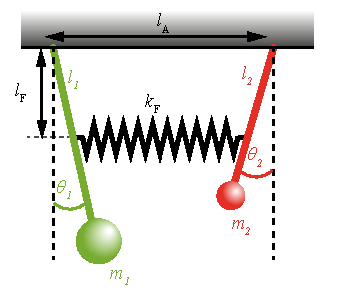
\includegraphics[width=0.5\textwidth]{GekoppeltePendel01.pdf}}%
\hspace{\fill}
\rightfigure{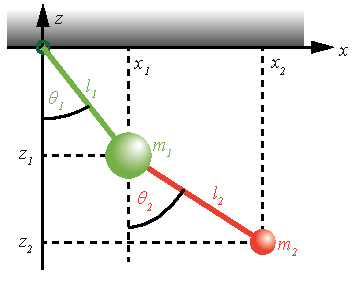
\includegraphics[width=0.5\textwidth]{DoppelPendel01.pdf}}
\leftcaption[Gekoppelte Stangenpendel.]{Gekoppelte Stangenpendel, die in der H�he $l_\text{F}$ durch eine Feder verbunden sind.}\label{abb:bew_Kopplg01}
\rightcaption{Geometrie des Doppelpendels.}\label{abb:bew_Doppelpendel01}
\end{minipage}
\end{figure}

Wir betrachten \figref{bew_Kopplg01} und bleiben zun�chst im Bereich geringer Auslenkungen.
Die Lagrange-Funktion lautet zun�chst ohne N�herungen
    \begin{align}
        \mathcal{L} &= \underbrace{\frac{m_1}{2} {l_1}^2 {\dot{\theta}_1{}}^2 + \frac{m_2}{2} {l_2}^2 {\dot{\theta}_2{}}^2}_T
        - g\,\underbrace{\lk  -m_1\, l_1\, \cos\theta_1 -m_2\,l_2\,\cos \theta_2 \rk}_{U_\text{Pendel}} \nonumber \\
        &\quad - \underbrace{\frac{k}{2} {l_\text{F}}^2 \lk (\sin\theta_1 - \sin\theta_2)^2 + (\cos\theta_1 - \cos\theta_2)^2\rk}_{U_\text{Feder}} 
        \label{eq:bew_Kopplg09} ~.
    \end{align}
Wir machen jetzt die N�herung
$l_i \sin\theta_i \approx l_i \theta_i$, sowie $\cos\theta_i \approx 1-\tfrac{{\theta_i}^2}{2} \approx 1$ und $l_\text{A} \geqq l_\text{F}$.
Zudem treffen wir die Annahmen
    \begin{align*}
        l_1 = l_2 = l_\text{F} \qquad \text{und} \qquad m_1 = m_2 = m~.
    \end{align*}
Wir erhalten damit f�r das vereinfachte und linearisierte Problem die Lagrange-Funktion in Matrix-Schreibweise
    \begin{align}
		\begin{split}
        \mathcal{L} =  
        \begin{pmatrix}
          \dot{\theta}_1 \\
          \dot{\theta}_2
        \end{pmatrix}^T
        \underbrace{
        m \,{l_\text{F}}^2 \begin{pmatrix}
        1 & 0 \\
        0 & 1
        \end{pmatrix}}_\mathbb{T}
        \begin{pmatrix}
          \dot{\theta}_1 \\
          \dot{\theta}_2
        \end{pmatrix}
        - 	
        \begin{pmatrix}
          \theta_1 \\
          \theta_2
        \end{pmatrix}^T
        \underbrace{ m \,g\,l_\text{F} 
        \begin{pmatrix}
          1 & 0 \\
          0 & 1
        \end{pmatrix}}_{\mathbb{U}_1}
        \begin{pmatrix}
          \theta_1 \\
          \theta_2
        \end{pmatrix} 
        \,- \begin{pmatrix}
          \theta_1 \\
          \theta_2
        \end{pmatrix}^T
        \underbrace{ k \,{l_\text{F}}^2 
        \begin{pmatrix}
          1 & -1 \\
          -1 & 1
        \end{pmatrix}}_{\mathbb{U}_2}
        \begin{pmatrix}
          \theta_1 \\
          \theta_2
        \end{pmatrix},
       \end{split} \label{eq:bew_Kopplg10}
    \end{align}
worin 
	$
        \begin{pmatrix}
                . \\
                .
        \end{pmatrix}
^T
$
	den transponierten Vektor darstellt.
Man erkennt an der Zerlegung von $\mathbb{U} = \mathbb{U}_1 + \mathbb{U}_2$, dass $\mathbb{U}_2$ nicht diagonal ist und die Kopplungsterme enth�lt.
Wir l�sen die charakteristische Gleichung \eqref{eq:bew_Kopplg08}:
    \begin{equation}
        {l_\text{F}}^2 \lk (m\,g + k \,l_\text{F} - m \,l_\text{F} \,\lambda)^2 - k^2\,{l_\text{F}}^2\rk = 0 \label{eq:bew_Kopplg11}~.
    \end{equation}
Diese hat als L�sungen die Eigenwerte
    \begin{align*}
        \lambda_1 = {\omega_1}^2 = \frac{g}{l_\text{F}} \qquad \text{und} \qquad \lambda_2 = {\omega_2}^2 =\frac{g}{l_\text{F}} + 2 \frac{k}{m}~.
     \end{align*} 
Die dazugeh�rigen Eigenvektoren bestimmen sich aus \eqref{eq:bew_Kopplg07}:
\[
\begin{pmatrix}
   m\,g\,l_\text{F} + k\,{l_\text{F}}^2 - \lambda_i\,m\,{l_\text{F}}^2  & -k\,{l_\text{F}}^2 \\
  - k\,{l_\text{F}}^2  & m\,g\,l_\text{F} + k \,{l_\text{F}}^2 - \lambda_i\,m \,{l_\text{F}}^2
\end{pmatrix}
\vec{n}_i = 0 ~~\text{und}~~\vec{n}_i= 	\begin{pmatrix}
  n_{1,i} \\
  n_{2,i}
\end{pmatrix} \,.
\]
Damit ergibt sich f�r den Eigenwert $\lambda_1$
\begin{align}
    \begin{pmatrix}
      +k\,{l_\text{F}}^2 &	-k\, {l_\text{F}}^2 \\
      - k\, {l_\text{F}}^2  & +k\, {l_\text{F}}^2
    \end{pmatrix}
    \begin{pmatrix}
      n_{1,1} \\
      n_{2,1}
    \end{pmatrix}
    &= 0 \qquad \implies \vec{n}_1 = \begin{pmatrix}
      1 \\1
    \end{pmatrix}
            \label{eq:bew_Kopplg12}\\
\intertext{und analog f�r $\lambda_2$}
        \begin{pmatrix}
          - k\,{l_\text{F}}^2 	& -k\,{l_\text{F}}^2 \\
          - k\,{l_\text{F}}^2 	& -k\,{l_\text{F}}^2
        \end{pmatrix}
        \begin{pmatrix}
          n_{1,2} \\ n_{2,2}
        \end{pmatrix}
        &= 0 \qquad \implies \vec{n}_2 = \begin{pmatrix} 1 \\ -1 \end{pmatrix}
        \label{eq:bew_Kopplg13}~.
\end{align}
Wir k�nnen die beiden Eigenschwingungen noch normalisieren, \dh wir fordern
\[
  {\vec{n}_i}^T ~ \mathbb{T} ~ \vec{n}_j = \delta_{ij}
\] 	 	
und erhalten schlie�lich die �berlagerung der beiden Normalschwingungen
\begin{equation}
    \begin{pmatrix}
      \theta_1(t) \\
      \theta_2(t)
    \end{pmatrix}
    = C_1 
    \begin{pmatrix} 1 \\ 1 \end{pmatrix} 
    \cos(\omega_1 t - \delta_1) 
    + C_2 
    \begin{pmatrix} 1 \\ -1 \end{pmatrix} 
    \cos(\omega_2 t - \delta_2) ~, \label{eq:bew_Kopplg14}
\end{equation}
wobei sich die Konstanten $C_1, C_2, \delta_1$ und $\delta_2$ aus den Anfangsbedingungen ergeben.
F�r eine passende Anfangsbedingung ist die L�sung von \eqref{eq:bew_Kopplg13} in \figref{bew_Kopplg02} gezeigt. Deutlich erkennt man das Auftreten einer Schwebung zwischen den Normalschwingungen.
Mit der Schwebung wandert die Energie quasi zwischen den beiden Pendeln hin und her.
Die numerische Rechnung (\mscr{} \mlbewref{GekoppeltePendel01.m}) zeigt f�r Winkel $<\SI{15}\degree$ gute �bereinstimmung mit \eqref{eq:bew_Kopplg14}.

\begin{figure}
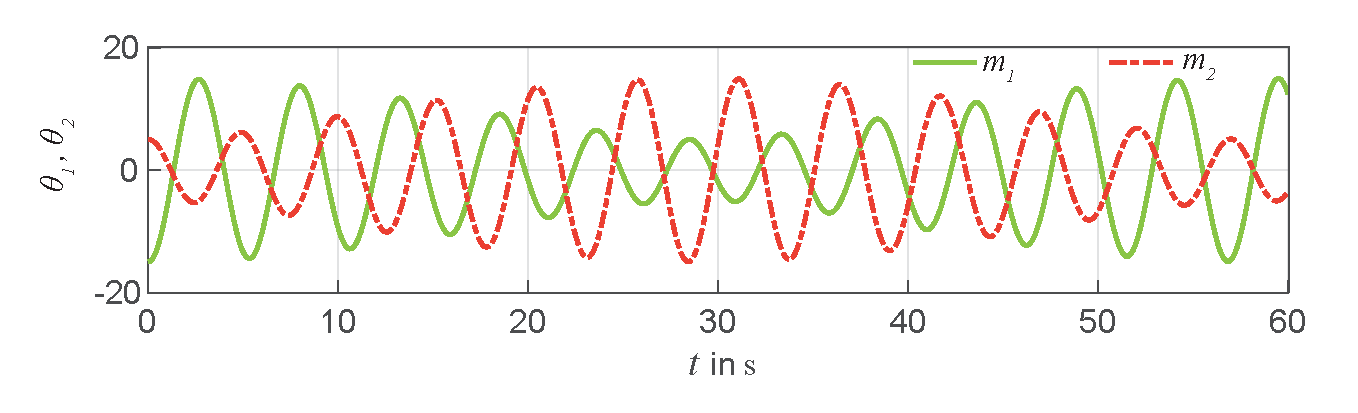
\includegraphics[width=\textwidth]{GekPendel01.pdf}%
\caption[Schwingungsverhalten zweier gekoppelter Stangenpendel.]{Schwingungsverhalten zweier gekoppelter Stangenpendel im Kleinwinkelfall und bei schwacher Kopplung. Deutlich ist das Schwebungsverhalten zu erkennen.}
\label{abb:bew_Kopplg02}
\end{figure}

Bisher haben wir uns in unserer Analyse auf kleine Winkel beschr�nkt und dar�ber hinaus gleiche Pendell�ngen und -massen angenommen.
Wir lassen nun f�r \probref{bew_Kopplung01} diese Begrenzungen fallen.
Die Rechnungen mit dem \mscr{} \mlbewref{GekoppeltePendel02.m} ergeben auch in diesem Fall f�r nicht zu starke Kopplungen $\keff$ das charakteristische Schwebungsverhalten (\figref{bew_Kopplg03}). Ebenso instruktiv ist es, in dem \mscr{}\, verschiedene Parameter wie \zb $\keff$ oder die relativen Pendell�ngen $l_1,\, l_2$ und -massen $m_1,\, m_2$ zu ver�ndern.

\begin{figure}
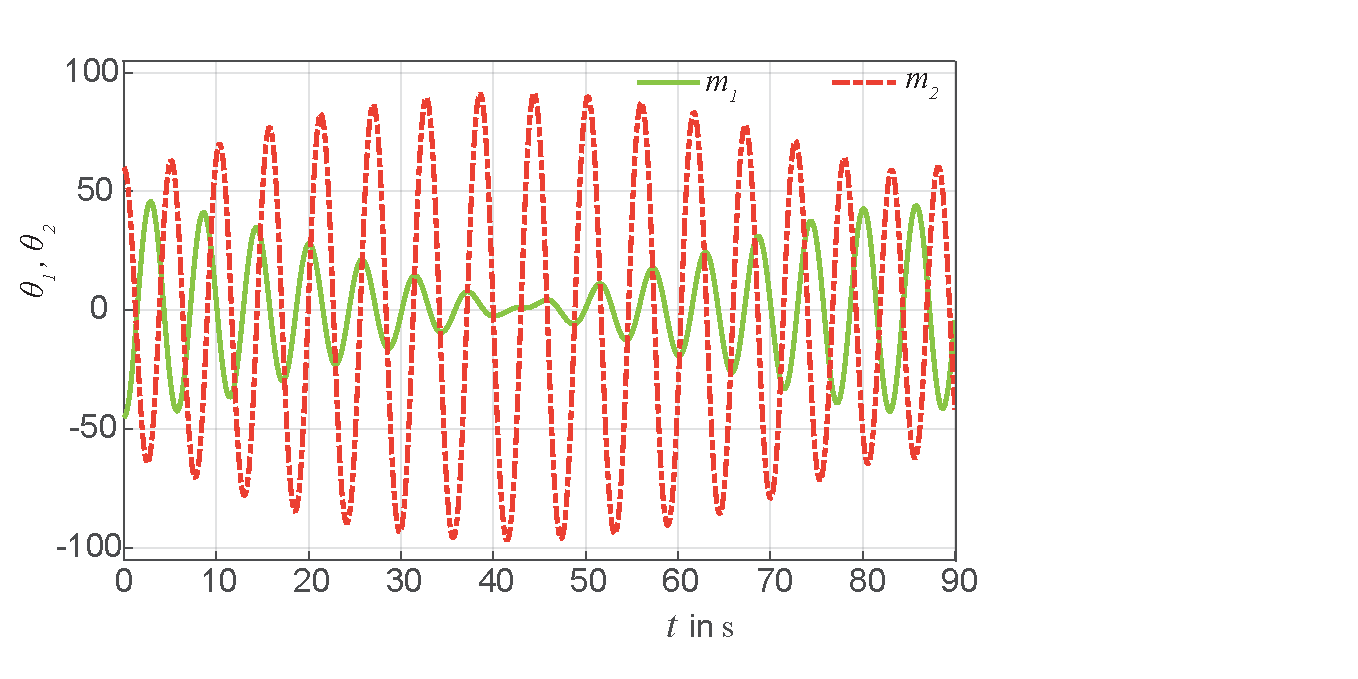
\includegraphics[width=\textwidth]{GekPendel02.pdf}%
\caption[Auslenkungen eines gekoppelten Pendels bei gro�en Auslenkungen.]{Auslenkungen eines gekoppelten Pendels bei gro�en Auslenkungen und schwacher Kopplung f�r folgende Parameter: $l_1 = \SI8\metre$, $l_2 = \SI6\metre$, $m_1 = \SI4{\kilo\gram}$, $m_2 = \SI3{\kilo\gram}$, $C_1 = 0.5$, $C_2 = 1$. Auch hier ist das Schwebungsverhalten deutlich zu erkennen.}
\label{abb:bew_Kopplg03}
\end{figure}

\subparagraph{Doppelpendel}

Diese Art des gekoppelten Pendels kann bei gr��eren Amplituden ein interessantes Verhalten zeigen, das auch als \anf{chaotisches Verhalten} bezeichnet wird.
Bevor wir dieses genauer anschauen, wollen wir die Bewegungsgleichungen des Doppelpendels aufstellen.
Unter Ber�cksichtigung der Zwangsbedingungen (\probref{bew_Zwangsbedingungen}) ergibt sich mit den generalisierten Koordinaten $\theta_1$ und $\theta_2$ die Lagrange-Funktion des Doppelpendels zu
\begin{align}
	\mathcal{L} &= \frac{m_1 + m_2}{2}\, {l_1}^2 \dot{\theta}_1{}^2 
	+ \frac{m_2}{2} {l_2}^2 \,{\dot{\theta}_2}{}^2 
	+ 2\,m_2 \,l_1\, l_2 \,\dot{\theta}_1 \,\dot{\theta}_2 \,\cos(\theta_1 - \theta_2) \nonumber \\
	&\quad + (m_1 + m_2) \,g \,l_1 \, \cos(\theta_1)
	+ m_2 \,g \,l_2 \,\cos(\theta_2) \,,\label{eq:bew_Doppelpendel01}
\end{align}
wobei wir konstante Terme im Potential \anf{weggeeicht} haben. 
Daraus lassen sich die Bewegungsgleichungen �ber
\[
\frac{\d \mathcal{L}}{\d t} \frac{\partial \mathcal{L}}{\partial \dot{\theta_i}} - \frac{\partial \mathcal{L}}{\partial \theta_i} = 0
\]
herleiten.
Man kann dabei gut von der symbolischen Toolbox von \matlab{} Gebrauch machen (siehe auch \mscr{} \mlbewref{Doppelpendel01.m}).
Wir erhalten
\begin{align}
	\ddot{\theta}_1 + \frac{g}{l_1}\,\sin\theta_1 + \frac{m_2}{m_1+m_2} \frac{l_2}{l_1} \
	\lek \ddot{\theta}_2\,\cos(\theta_2 - \theta_1) - {\dot{\theta}_2}{}^2 \,\sin(\theta_2 - \theta_1)  \rek 
	&= 0 \nonumber \quad \text{und}\\
	\ddot{\theta}_2 + \frac{g}{l_2}\sin\theta_2 + \frac{l_1}{l_2} \frac{m_1}{m_2} 
	\lek \ddot{\theta}_1 \,\cos(\theta_2 - \theta_1) - {\dot{\theta}_1}{}^2 \,\sin(\theta_2 - \theta_1)  \rek
	&= 0
	\label{eq:bew_Doppelpendel02}~.
\end{align}
Man erkennt an der Struktur der Lagrange-Gleichungen sehr sch�n, dass die beiden Pendelschwingungen durch die nichtlinearen Kopplungsterme (in den eckigen Klammern) gest�rt werden. 
F�r spezielle F�lle k�nnen wir aus \eqref{eq:bew_Doppelpendel02} wieder das sogenannte \anf{Kleinwinkelverhalten}, also die Bewegung bei geringen Auslenkungen, analytisch berechnen.
Wir nehmen dabei den einfachen Fall
\begin{align*}
	m_1 = m_2 = m 
	\quad \text{und} \quad 
	l_1=l_2 = l,
	\quad \text{sowie} \quad 
	\theta_1, \theta_2 \leqq 5\degree
\end{align*}
an, sodass gilt:
\begin{align*}
	\cos\theta_i &\approx 1~~~\text{und}~~~ \sin\theta_i \approx \theta_i,
	\quad {\dot{\theta_i}}^2 \theta_i \approx 0~.
\end{align*}
Die Lagrange-Gleichungen \eqref{eq:bew_LagrangeGl_II} vereinfachen sich damit erheblich zu
\begin{align}
	\ddot{\theta}_1 + \frac{g}{l} \theta_1 + \frac{1}{2} \ddot{\theta}_2 &= 0 \nonumber \\
	\ddot{\theta}_1 + \frac{g}{l} \theta_2 + \ddot{\theta}_2 &= 0~, 	\label{eq:bew_Doppelpendel03a}
\end{align}
\bzw in Matrixform
\begin{align}
    \begin{pmatrix}
 	 1  & 1/2 \\
	 1  & 1  
    \end{pmatrix}
    \begin{pmatrix}
 	\ddot{\theta}_1\\
 	\ddot{\theta}_2
    \end{pmatrix}
\, + \,
    \begin{pmatrix}
 	 g/l  & 0 \\
	 0    & g/l  
    \end{pmatrix}
    \begin{pmatrix}
 	\theta_1\\
 	\theta_2
    \end{pmatrix}
\, &= \, 0 \,.	\label{eq:bew_Doppelpendel03b}
\end{align}
Wir haben offensichtlich in dieser N�herung das DGL-System \textit{linearisieren} k�nnen und k�nnten damit nun einen der klassischen L�sungsans�tze (wie $\theta_i = \hat{\theta}_i \cos(\omega t)$) verfolgen.
Wir wollen hier aber bewusst die in diesem Kapitel eingef�hrte Methode �ber die charakteristische Gleichung \eqref{eq:bew_Kopplg08} verwenden. 
\Dh wir beginnen mit der Matrixform \eqref{eq:bew_Doppelpendel03b} und berechnen daraus direkt die Eigenfrequenzen $\lambda_{1,2} = (\omega_{1,2})^2$.
Die charakteristische Gleichung lautet dann\footnote{Als instruktive �bung wird empfohlen zu zeigen, dass die Ansatzmethode zu demselben Ergebnis f�hrt.}
\begin{equation}
    \begin{vmatrix}
	g/l - \lambda& -\lambda/2 \\
	-\lambda & g/l-\lambda
    \end{vmatrix} = 0 \label{eq:bew_Doppelpendel05}~. 
\end{equation}
Sie f�hrt uns zu den beiden Eigenwerten
\begin{equation}
	\lambda_{1,2} = {(\omega_{1,2})}^2 = \lk 2 \pm \sqrt{2}\rk \frac{g}{l} = \lk 2 \pm \sqrt{2}\rk {\omega_0}^2 \label{eq:bew_Doppelpendel06}~.
\end{equation}
Die Eigenmoden bestimmen wir �ber \eqref{eq:bew_Kopplg07}:\footnote{Alternativ setzt man die $\omega_i$ mit dem Ansatz in \eqref{eq:bew_Doppelpendel06} ein.
Wir erhalten dann f�r $\omega_1\!: \hat{\theta}_{2}^{(1)} = - \sqrt{2}\,\hat{\theta}_{1}^{(1)} $
und f�r $\omega_2\!: \hat{\theta}_{2}^{(2)} = + \sqrt{2}\,\hat{\theta}_{1}^{(2)}$.}
\[
\omega_1\,\text{:} ~n_{2,1} = - \sqrt{2}\,n_{1,1} ~~ \text{und} ~~ \omega_2 \,\text{:} ~n_{2,2} = + \sqrt{2}\,n_{1,2}\,.
\]
Das bedeutet, dass die beiden Pendel bei $\omega_1=\omega_\text{a}$ antisymmetrisch (also entgegengesetzt) schwingen und bei $\omega_2=\omega_\text{s}$ symmetrisch (also gleichgerichtet).
Die antisymmetrische Schwingungsfrequenz $\omega_\text{a}$ ist nach \eqref{eq:bew_Doppelpendel06} $1 + \sqrt{2} \approx 2.4$-fach so hoch wie die der symmetrischen Schwingung.
Das l�sst sich leicht verstehen, da die r�cktreibenden Kr�fte im antisymmetrischen Fall gr��er sind.
Im Rahmen der Kleinwinkeln�herung ist die allgemeine L�sung also durch eine �berlagerung der beiden Normalschwingungen gegeben:
\begin{align*}
    \begin{pmatrix}
 	\theta_1\\
 	\theta_2
    \end{pmatrix}
\, = \,
    \begin{pmatrix}
 	n_{1,1} & n_{1,2}\\
 	n_{2,1} & n_{2,2}
    \end{pmatrix} 
    \begin{pmatrix}
 	C_1\, \cos(\omega_\text{a} t + \delta_\text{a})\\
 	C_2\, \cos(\omega_\text{s} t + \delta_\text{s}) 
    \end{pmatrix}
\end{align*}
\bzw in komplexer Schreibweise
\begin{align}
	\theta_1(t) &= \lk A \text{e}^{\mathrm{i} \omega_\text{a} t} + B \text{e}^{-\mathrm{i}\omega_\text{a} t}\rk + \lk C \text{e}^{\mathrm{i}\omega_\text{s} t} + D \text{e}^{-\mathrm{i}\omega_\text{s} t} \rk \;,\nonumber \\
	\theta_2(t) &= -\sqrt{2} \lk A \text{e}^{\mathrm{i} \omega_\text{a} t} + B \text{e}^{-\mathrm{i}\omega_\text{a} t}\rk + \sqrt{2} \lk C \text{e}^{\mathrm{i}\omega_\text{s} t} + D \text{e}^{-\mathrm{i}\omega_\text{s} t} \rk \label{eq:bew_Doppelpendel07}~. 
\end{align}
W�hlen wir die Anfangsbedingungen \zb zu
\begin{align*}
	\theta_1(0) &= \theta_{10} = +(A+B) + (C+D) \,,\\
	\theta_2(0) &=\theta_{20} = -\sqrt{2} (A+B) + \sqrt{2} (C+D) \,,\\
	\dot{\theta}_1(0) &= \dot{\theta}_{10} = + \im\, \omega_\text{a} (A-B) + \im\, \omega_\text{s} (C-D) \,,\\
	\dot{\theta}_2(0) &= \dot{\theta}_{20} = - \im \sqrt{2}\, \omega_\text{a} (A-B) + \im \sqrt{2}\, \omega_\text{s} (C-D)\,, \\
\end{align*}
so ergibt sich
\begin{equation}
    \begin{pmatrix}
	+1 & +1 & +1 & +1 \\ 
	-1 & -1 & +1 & +1 \\
	+\mathrm{i} \omega_\text{a} & -\mathrm{i}\omega_\text{a} & +\mathrm{i}\omega_\text{s} & -\mathrm{i}\omega_\text{s} \\
	-\mathrm{i} \omega_\text{a} & +\mathrm{i}\omega_\text{a} & +\mathrm{i}\omega_\text{s} & -\mathrm{i}\omega_\text{s}
    \end{pmatrix}
    \begin{pmatrix} A \\ B\\ C\\ D\end{pmatrix}
    = 
    \begin{pmatrix}
	\theta_{10} \\ \theta_{20} /\sqrt{2} \\ \dot{\theta}_{10} \\ \dot{\theta}_{20} /\sqrt{2}
    \end{pmatrix}~.
\end{equation}
Wir l�sen dieses lineare Gleichungssystem in \matlab{} und erhalten die Werte der Koeffizienten $A$, $B$, $C$ und $D$. 
Damit k�nnen wir schlussendlich die Kleinwinkell�sung nach \eqref{eq:bew_Doppelpendel07} bestimmen. Diese vergleichen wir f�r $\theta_1, \theta_2 \leqq 5\degree$
mit der numerischen L�sung aus dem  \mscr{} \mlbewref{Doppelpendel02.m} und finden eine gute �bereinstimmung.\\

\begin{figure}
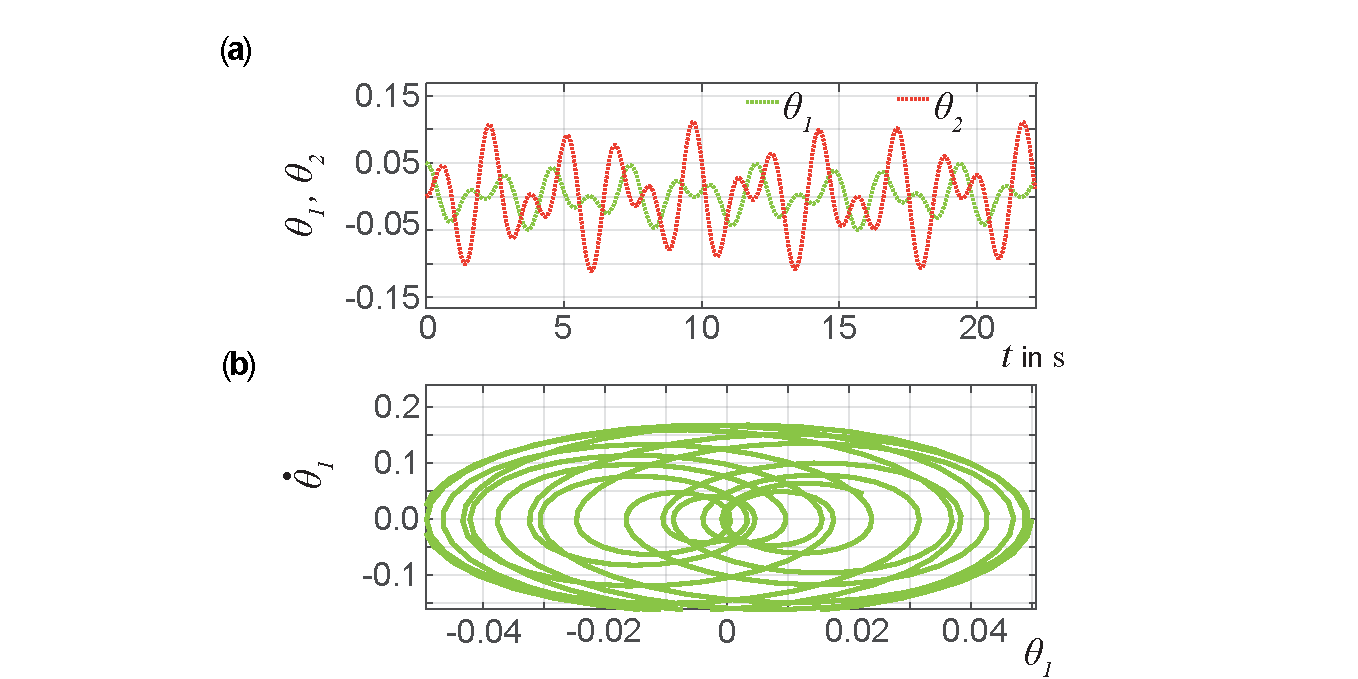
\includegraphics[width=\textwidth]{DoppelPendel03.pdf}%
\caption[Kleinwinkelverhalten des Doppelpendels.]{Kleinwinkelverhalten des Doppelpendels. \fa Bei geringen Auslenkungen zeigt das Doppelpendel mehr oder weniger ein Schwebungsverhalten, \dh die Energie wandert �ber die Zeit zwischen den beiden Pendelarmen hin und her. 
Im Bild ist die analytische N�herung nach \eqref{eq:bew_Doppelpendel07} f�r die entsprechenden Anfangsbedingungen dargestellt.
In der Zeitentwicklung der Auslenkungen der beiden Pendelarme erkennt man das Schwebungsverhalten aus den �berlagerungen der Eigenmoden. 
\fb Der Phasenraum zeigt eine geschlossene Kurve.}\label{abb:bew_Doppelpendel03}
\end{figure}

\subparagraph{\anf{Chaotisches Verhalten} des Doppelpendels}\index{Chaos}

Wir wollen nun das Doppelpendel bei gro�en Auslenkungen $\theta_1, \theta_2$ betrachten,
bei denen es zu chaotischem Verhalten neigt.
Im \mscr{} \mlbewref{Doppelpendel02.m} haben wir die Bewegungsgleichungen f�r das Doppelpendel numerisch mit der \matlab-Routine \odevf gel�st. Die Ergebnisse sind beispielhaft in \figref{bew_Doppelpendel02} dargestellt.
Die numerische L�sung zeigt, dass es au�erhalb des Bereichs, in dem die DGL \emph{linearisiert} wurden, unter bestimmten Bedingungen zu \emph{chaotischem Verhalten}\index{System!chaotisches} kommen kann.
Von \emph{Chaos} spricht man in der Physik, wenn bereits die kleinste �nderung der Anfangsbedingungen zu einem scheinbar v�llig anderen zeitlichen Verhalten f�hrt.%
\footnote{So eine kleine �nderung der Anfangsbedingungen kann \zb auch durch Ungenauigkeiten bei der numerischen Rechnung eintreten. Man mache sich aber klar, dass dies dennoch ein deterministisches Problem ist.}

Allgemein k�nnen wir festhalten, dass f�r chaotisches Verhalten die zugrundeliegenden Lagrange-Funktionen \bzw Bewegungsgleichungen nichtlineare Terme enthalten m�ssen.
Im Falle von \eqref{eq:bew_Doppelpendel02} sind dies die Terme
$\lek \ddot{\theta}_2\,\cos(\theta_2 - \theta_1) - {\dot{\theta}_2}{}^2 \,\sin(\theta_2 - \theta_1)  \rek$ und 
$\lek \ddot{\theta}_1 \,\cos(\theta_2 - \theta_1) - {\dot{\theta}_1}{}^2 \,\sin(\theta_2 - \theta_1)  \rek$
in der Lagrange-Funktion $\mathcal{L}$. 
Das chaotische Verhalten ist im Phasendiagramm $\lek \theta_i(t) \, ~~ \, \dot{\theta}_i(t) \rek$ von \figref{bew_Doppelpendel02} zu erkennen, w�hrend \figref{bew_Doppelpendel03} im Vergleich dazu das Verhalten bei kleineren Auslenkungen $\theta_1, \theta_2$ zeigt und wir hier ein weitgehend \anf{normales} Schwingungsverhalten erkennen.\\
Wir werden das Thema Chaos in \kap{bew_chaos} noch weiter vertiefen.
\begin{figure}
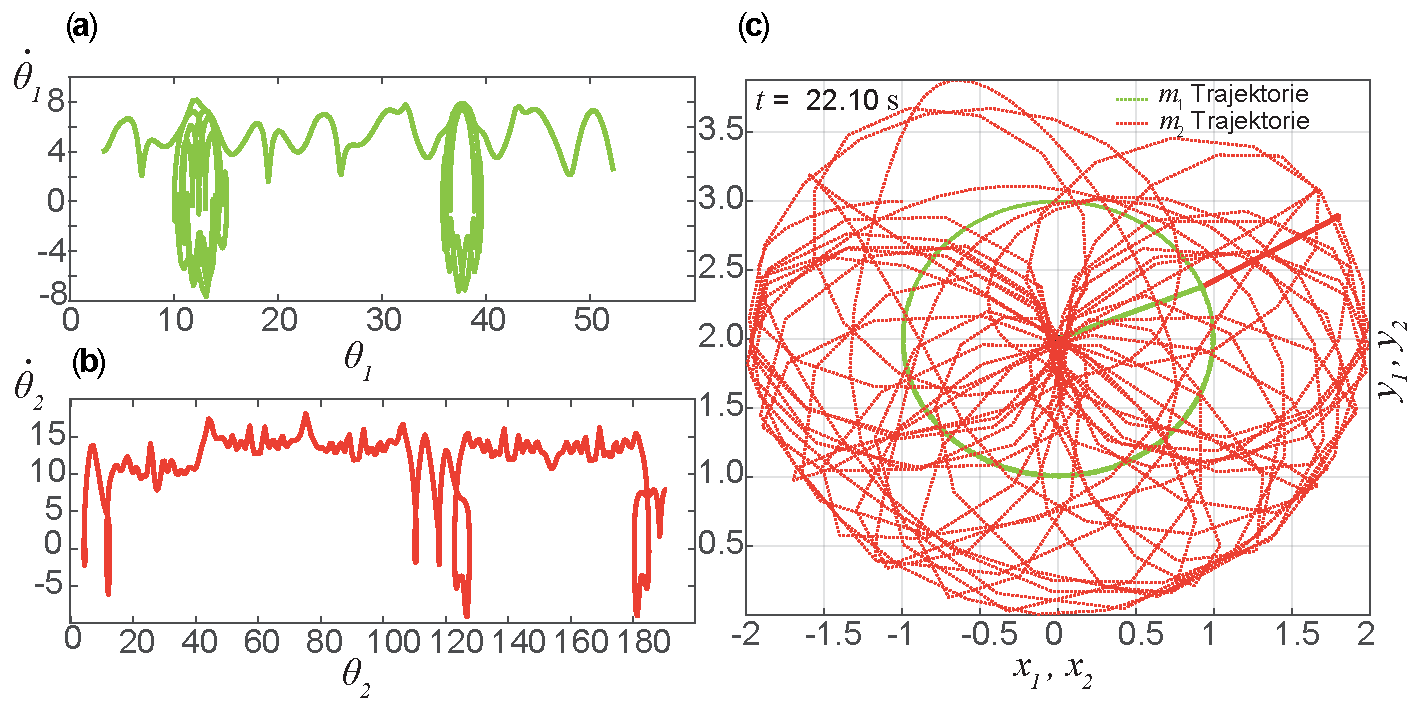
\includegraphics[width=\textwidth]{DoppelPendel02.pdf}%
\caption[Chaotisches Verhalten des Doppelpendels.]{Chaotisches Verhalten des Doppelpendels. \fa, \fb Phasenraum der beiden Pendelarme gezeigt (gr�n = Pendel 1, rot = Pendel 2). Man erkennt, dass es selbst nach l�ngerer Zeit keine geschlossene Kurve gibt, obwohl Energieerhaltung gilt. \fc \gls{traj}n der beiden Pendelarme in kartesischen KoordinatenFrequenzantwort eines Schwingungstilgers (. Die Unstetigkeiten sind durch die Schrittweite in der Darstellung bedingt. Die Zwangsbedingung f�r den Pendelarm 1 ist deutlich zu erkennen. Die Bewegungen der Pendelarme zeigen \anf{chaotisches} Verhalten (\mscr{} \mlbewref{DoppelPendel02.m}).}
\label{abb:bew_Doppelpendel02}
\end{figure}

\subsubsection{Schwingungstilgung}\index{Schwingungstilgung|textbf} \label{kap:bew_Tilgung}

\begin{figure}
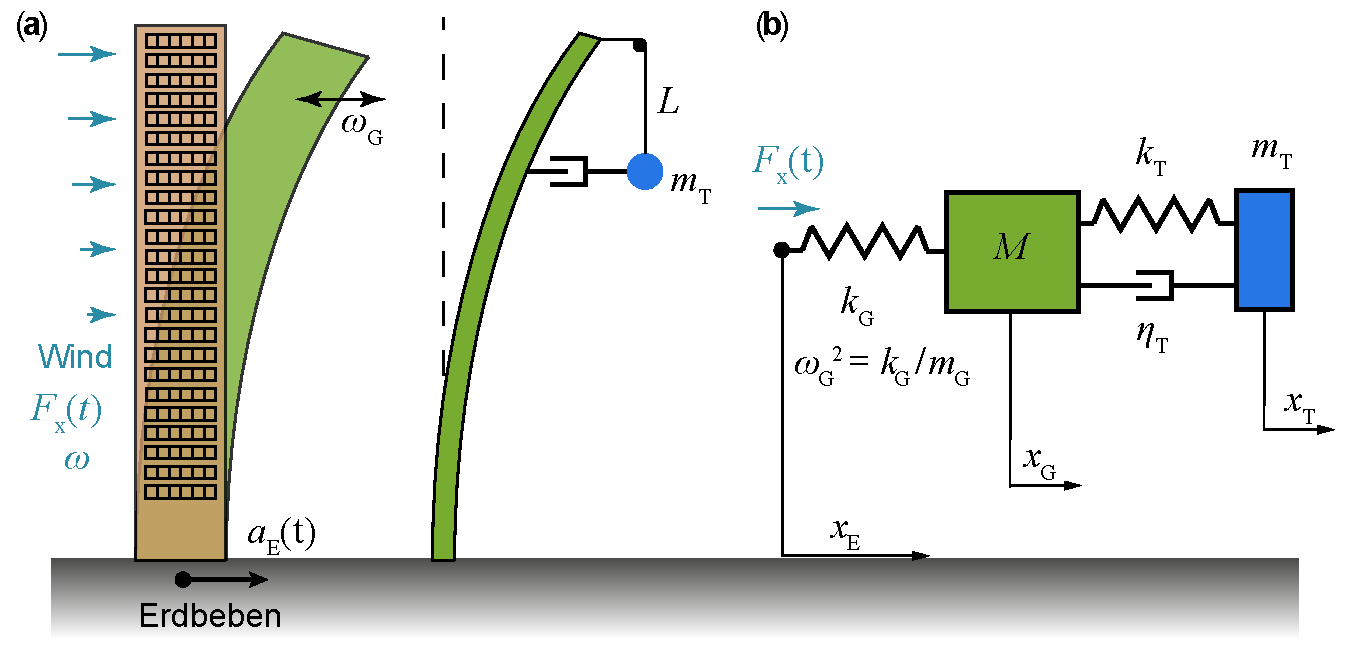
\includegraphics[width=\textwidth]{TilgungSchema.pdf}%
\caption[Schwingungstilgung an Geb�uden.]{Schwingungstilgung an Geb�uden. \fa Anregung durch Wind bzw. Erdbeben \fb Vereinfachtes Modell des Systems.}
\label{abb:bew_TilgungSchema}
\end{figure}

Ein besonders interessanter Fall der Schwingungskopplung sind die sogenannten \emph{Schwingungstilger}. Im Englischen werden diese auch sehr treffend \textit{Tuned Mass Damper} (TMD)\index{Tuned Mass Damper|textbf} oder auch \textit{Tuned Vibration Absorber} (TVA) genannt. Wir werden deshalb auch die Abk�rzung TMD verwenden. Bei diesen Schwingungstilgern wird ein passives Gegengewicht $m_\text{T}$ an eine Hauptmasse $M$ (\zb Geb�ude, Tisch wir benutzen hier zur besseren Unterscheidung den Gro�buchstaben) gekoppelt, deren Schwingungsverhalten bei bestimmten Anregungen unterdr�ckt \bzw ged�mpft werden soll. Es gibt zahlreiche Beispiele f�r solche TMDs, insbesondere bei Hochbauten, so \zb in den USA den John Hancock Tower in Boston, in Deutschland den Berliner Fernsehturm, den Testturm in Rottweil und in Taiwan das Taipei 101 Geb�ude. Die Idee ist, dass bei einer Schwingungsanregung der Hauptmasse, \zb durch Wind, der Tilger die Schwingungsenergie der Hauptmasse aufnimmt und dann d�mpft (\figref{bew_TilgungSchema}a). Dazu muss dieser auf die erwartete externe Anregungs-Schwingungsfrequenz abgestimmt werden. 
Das einfachste physikalische Modell f�r ein solches System zeigt \figref{bew_TilgungSchema}b. Man kann leicht die Lagrange-Funktion $\mathcal{L} = T-U$ und die Dissipationsfunktion aufschreiben und daraus die Bewegungsgleichung herleiten:\footnote{Hier haben wir der Einfachheit halber die D�mpfung der Struktur als klein gegen $\eta_\text{T}$ angenommen und diese wiederum als proportional zur Relativgeschwindigkeit beider Massen, da sich die D�mpfung zwischen den beiden Massen befindet.}
\begin{align}
\begin{split}
    M \,\ddot{x}_\text{M} + \eta_\text{T}\,\lk \dot{x}_\text{M} - \dot{x}_\text{T}\rk + k_\text{M}\,x_\text{M} - k_\text{T}\,\lk x_\text{T} - x_\text{M}\rk &= F_\text{x}\lk t\rk = \hat{F}_\text{x}\,\e_\text{x}^{i\omega t} \,, \\
    m_\text{T}\,\ddot{x}_\text{T} + \eta_\text{T}\,\lk \dot{x}_\text{T} - \dot{x}_\text{M}\rk + k_\text{T}\, \lk x_\text{T} -x_\text{M}\rk &= 0 \,.
\end{split} \label{eq:bew_TilgungBasic01}
\end{align}
Darin sind $M, \eta_\text{M}, k_\text{M}$ durch die Geb�udestruktur vorgegebene Gr��en, ebenso sei $F_\text{x}\lk t\rk$ (\bzw im Frequenzbereich $\hat{F}_\text{x}\lk \omega\rk$) als externe Anregung bekannt.\footnote{Wir lassen erdbeben�hnliche St�rungen unber�cksichtigt, mit anderen Worten das Fundament des Geb�udes bleibt fix ($x_\text{G} = 0,\, a_\text{E} = 0\,.$).} Wir haben diese durch eine komplexe Funktion beschrieben, sodass die L�sungen $x_\text{M}(t), x_\text{T}(t)$ auch komplex werden, und damit neben der Amplitude auch die Phase relativ zur Anregung liefern. Die Frage ist, wie man mit den freien Parametern $m_\text{T}$, $\eta_\text{T}$ und $k_\text{T}$ einen optionalen Tilger (TMD) auslegt. Ziel muss es dabei sein,
\begin{enumerate}
    \item [a)] 
    das Geb�ude/die Struktur (Masse $M$) mit der Eigenfrequenz $\omega_\text{M} = \sqrt{k_\text{M}/M}$ \bzw der externen Anregungsfrequenz $\omega$ optimal zu d�mpfen, \dh die relative Amplitude $x_\text{M}/(F_\text{x}/M)$ so klein wie m�glich zu machen, und
    \item [b)]
    die unweigerlich durch das gekoppelte System zus�tzlich entstehenden Eigenschwingungen mit den Frequenzen $\omega_\text{u}$, $\omega_\text{o}$ so klein wie m�glich und so weit entfernt wie m�glich von $\omega_\text{M}$ auftreten zu lassen. 
\end{enumerate}
Dieses Optimierungsproblem wird zu einem Kompromiss f�hren, da a) und b) gegeneinander \anf{laufen}.
Das kann man sich leicht �berlegen, indem man im DGL-System \eqref{eq:bew_TilgungBasic01} $\,\eta_\text{M} = 0$ und $k_\text{T}/m_\text{T} = k_\text{M}/M = \omega^2$ setzt.
Dann sind die verbleibenden freien Parameter des TMD das Masseverh�ltnis $\gamma= m_\text{T}/M$ und die D�mpfung der Tilgungsmasse $\eta_\text{T}$.
Wir wollen den Einfluss dieser beiden  Parameter auf das Schwingungsverhalten auf Basis der DGL \eqref{eq:bew_TilgungBasic01} berechnen.%
\footnote{In der Literatur finden sich h�ufig leicht verschiedene Bewegungsgleichungen f�r den TMD. Die Unterschiede r�hren vor allem von der unterschiedlichen Verwendung der KOS f�r die beiden bewegten Massen her. Wie haben bei der Herleitung von \eqref{eq:bew_TilgungBasic01} jeweils den $0$-Punkt der Koordinaten in die Ruhelage der Struktur ($x_\text{M}$-Koordinate) \bzw des Tilgers ($x_\text{T}$-Koordinate) gelegt.} \\
Wir sind unter der Annahme einer periodischen Anregung (\zb durch Windb�en) an der station�ren L�sung des gekoppelten Systems interessiert. Dazu machen wir wieder den bereits bekannten Exponentialansatz%
\footnote{Wir k�nnen auch sagen, dass wir das System im Frequenzbereich betrachten und dazu eine Fourier-Transformation der DGL machen. Siehe dazu die \onlineZ \bzw  das Kapitel "`Physik der Musik"' im zweiten Band dieser Reihe, in denen wir uns intensiver mit dem Thema befassen werden.}:
\begin{align}
    x_\text{M} = \hat{X}_\text{M}\,\e^{\im\omega t}\,,~~~ x_\text{T} = \hat{X}_\text{T}\,\e^{\im\omega t} \,. \label{eq:bew_TilgungBasic02}
\end{align}
Das f�hrt auf das folgende lineare Gleichungssystem in $\hat{X}_\text{M}$ und $\hat{X}_\text{T}$:
\begin{align*}
    \hat{X}_\text{M}\,\lk -\omega^2\,M + \im\,\omega\,\eta_\text{M} + k_\text{M} + k_\text{T}\rk + \hat{X}_\text{T}\,\lk -\im\,\omega\,\eta_\text{T} - k_\text{T}\rk &= F_\text{x} \,,\\
    \hat{X}_\text{M}\,\lk -\im\,\omega\,\eta_\text{T} - k_\text{T}\rk + \hat{X}_\text{T}\,\lk -\omega^2\,m_\text{T} + \im\,\omega\,\eta_\text{T} + k_\text{T} \rk &= 0\,.
\end{align*}
Wir l�sen nach $\hat{X}_\text{M}$ und finden
\begin{align}
    \hat{X}_\text{M}(\omega) = \frac{F_\text{x}\lk -\omega^2\,m_\text{T} + \im\,\omega\,\eta_\text{T} + k_\text{T}\rk}{NN} \label{eq:bew_TilgungBasic03} 
\end{align}
mit
\begin{align*}
    NN = \lk -\omega^2\,M + \im\,\omega\,\eta_\text{M} + k_\text{M} + k_\text{T}\rk\lk -\omega^2\,m_\text{T} + \im\,\omega\,\eta_\text{T} + k_\text{T}\rk - \lk \im\,\omega\,\eta_\text{T} + k_\text{T}\rk^2  \; .
\end{align*}
Die sogenannte \gls{frequenzantwort} (Englisch: \textit{Frequency Response} $R\lk\omega\rk$) des Systems auf die Anregung mit der Frequenz $\omega$ ist dann: 
\begin{align}
    R\lk\omega\rk = \frac{k_\text{M}\,\hat{X}_\text{M}\lk\omega\rk}{\hat{F}_\text{x}} \; . \label{eq:bew_TilgungBasic04} 
\end{align}
Diese Frequenzantwort ist eine komplexe Gr��e. Wir sind zun�chst nur an ihrem Betrag interessiert, den wir aus \eqref{eq:bew_TilgungBasic03} numerisch (\mscr{} \mlbewref{Tilgung01.m}) berechnen.\\
%Wir erhalten:
%\begin{align}
%\begin{split}
    %|R\lk \omega\rk|^2 &= R\lk \omega\rk\,R^*\lk\omega\rk \\
    %|R\lk \omega\rk|   &= \frac{1}{c^2+d^2}\,\sqrt{\lk ac+bd\rk^2 + \lk bc-ad\rk^2}~~~\text{mit} \\ 
    %a &= -\omega^2\,m_\text{T} + k_\text{T} \\
    %b &= \omega\,\eta_\text{T} \\
    %c &= \omega^4\,M\,m_\text{T} - \omega^2\,\lk k_\text{M}\,m_\text{T} + k_\text{T}\,m_\text{T}\rk + k_\text{M}\,k_\text{T} \\
    %d &= -\omega^3\,\eta_\text{T}\,\lk M + m_\text{T}\rk - \omega^2\,M\,k_\text{T} + \omega\,\eta_\text{T}\,k_\text{M}
%\end{split} \label{eq:bew_TilgungBasic05} 
%\end{align}
Wir k�nnen uns nun einige Spezialf�lle �berlegen:
\begin{itemize}
    \item $\eta_\text{T} \rightarrow \infty$: Der Tilger ist dann quasi starr an die Struktur gekoppelt, die Eigenfrequenz der Struktur wird sich leicht verschieben zu $\omega_\text{M}{}' = \sqrt{k_\text{M}/\lk M + m_\text{T}\rk}$.
    \item $\eta_\text{T} \rightarrow 0$: In diesem Fall gilt $R\lk \omega\rk = 0$ f�r $\omega = \omega_\text{T} = \sqrt{k_\text{T}/m_\text{T}}$.
\end{itemize}
F�r den Spezialfall $\eta_\text{T} = 0$ zeigt \figref{bew_TilgungBasic01}a die Frequenzantwort f�r verschiedene Massenverh�ltnisse $\gamma= m_\text{T}/M$ und \figref{bew_TilgungBasic01}b die Frequenzantwort f�r verschiedene $\eta_\text{T}$ bei konstantem Massenverh�ltnis $\gamma= 0.05$.
\figref{bew_TilgungBasic02} zeigt die Frequenzantwort $|R\lk\omega\rk|$ f�r verschiedene Abstimmungen (\dh D�mpfungen) eines TMD mit dem Masseverh�ltnis $\gamma = \SI{0.1}{}$ und einer D�mpfung von $\eta_\text{T} = \SI{0.05}{\kg\per\second}$. 

\begin{figure}
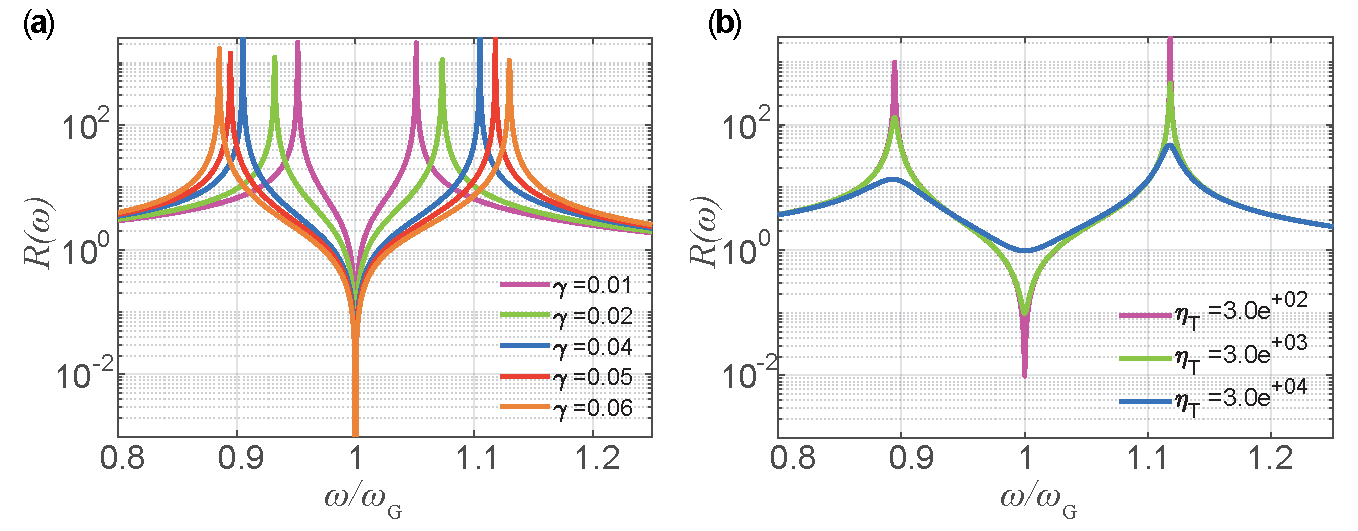
\includegraphics[width=\textwidth]{TilgungBasic01.pdf}%
\caption[Frequenzantwort eines Schwingungstilgers.]{Frequenzantwort eines Schwingungstilgers (TMD) f�r verschiedene Parameter. Linkes Bild: Verschiedene Massenverh�ltnisse $\gamma$ und $\eta_\text{T} = 0$. Rechtes Bild: Verschiedene D�mpfungen $\eta_\text{T}$ in $\SI{}{\kg\per\s}$ und konstantes Massenverh�ltnis $\gamma = 0.05$.}
\label{abb:bew_TilgungBasic01}
\end{figure}

Worin besteht nun eine Optimierung, m.\,a.\,W.\ die richtige \anf{Abstimmung}  \bzw das richtige \anf{Tuning}? Wir verwenden hier das sogenannte \textit{Den Hartog-Verfahren} \cite{DenHartog1984}, dessen Vorgehen in Folgendem besteht:
\begin{enumerate}
    \item
    Man w�hlt ein passendes Masseverh�ltnis $\gamma =  m_\text{T}/M$. Dieses liegt typischerweise im Bereich $0.01 \ldots 0.05$. Man beachte, dass f�r $M$ die effektiv schwingende Masse eingesetzt wird. Die Eigenfrequenz $\omega_\text{M} = \sqrt{k/M}$ sei bekannt. 
    \item
    Man hat nun zwei freie Parameter, mit denen man die Frequenzantwort optimieren kann. N�herungsweise kann man f�r $\gamma < 0.05$ die optimale Eigenfrequenz des Tilgers $\omega_\text{T,opt}$ aus 
			\[\omega_\text{T,opt} \approx \sqrt{\frac{1-0.5\,\gamma}{1+\gamma}}\,\omega_\text{M}
	\]
	bestimmen. 
    \item
	Die optimale D�mpfung des Tilgers findet man bei 
    \begin{align*}
        \eta_\text{T,opt} = 2\,\omega_\text{T,opt}\,m_\text{T} \sqrt{\frac{\gamma\,\lk 3-\sqrt{0.5\,\gamma}\rk }{8\lk 1 +\gamma \rk \lk 1 - 0.5\,\gamma \rk}}\,.
    \end{align*}
\end{enumerate}
Die Frequenzantwort eines nach diesen Kriterien abgestimmten TMD ist ebenfalls in \figref{bew_TilgungBasic02} gezeigt. Wie man sieht, ist im Unterschied zum nicht abgestimmten TMD die Tilgung beim abgestimmten TMD im Bereich der Eigenfrequenz etwas geringer, daf�r \anf{verh�lt} sich aber das System insgesamt �ber einen gr��eren Frequenzbereich hinweg \anf{gutartiger}, \dh die Frequenzantwort ist �ber einen Bereich von etwa $0.9\,\omega_\text{M} - 1.1\,\omega_\text{M}$ relativ konstant. 

\begin{figure}
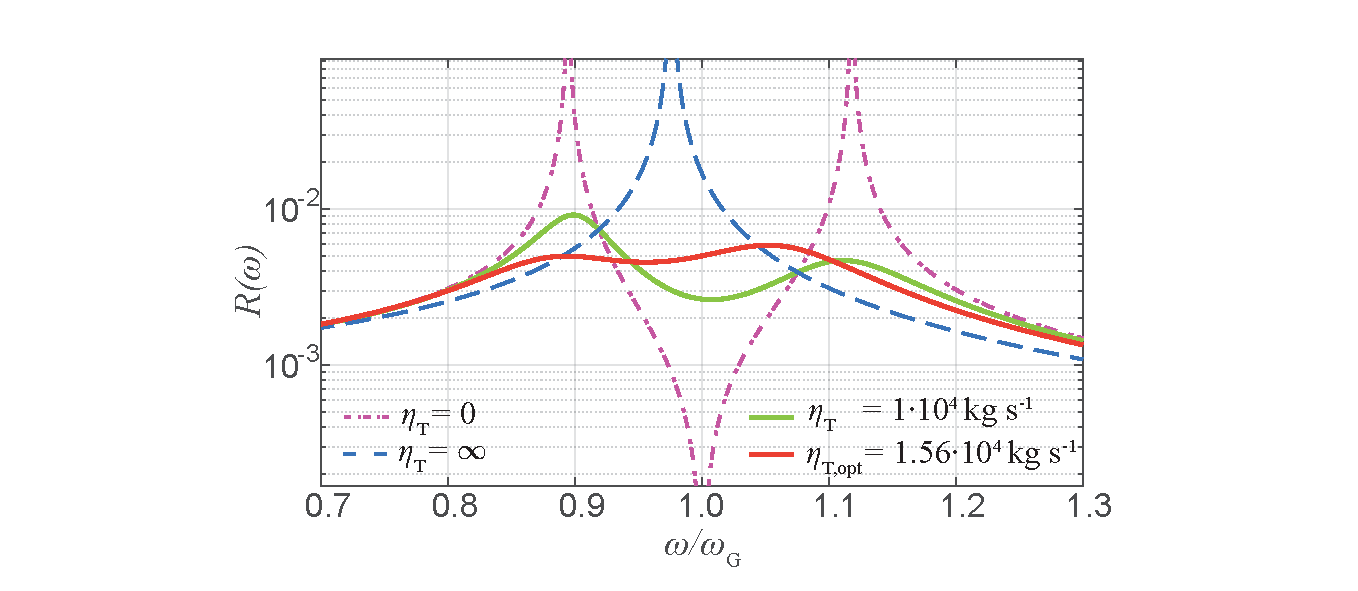
\includegraphics[width=\textwidth]{TilgungBasic02.pdf}%
\caption[Schwingungstilgung nach dem Den Hartog-Verfahren.]{Schwingungstilgung nach dem Den Hartog\footnote{Jacob Pieter Den Hartog (1901--1989) war ein niederl�ndisch-US-amerikanischer Ingenieurwissenschaftler f�r Mechanik, der 1940 die theoretischen Grundlagen f�r mechanische Schwingungstilger aufstellte.}\indexp{Den Hartog, Jacob Pieter}-Verfahren \cite{DenHartog1984}. Die rote durchgezogene Kurve zeigt den abgestimmten Schwingungstilger. }
\label{abb:bew_TilgungBasic02}
\end{figure}

In \probref{bew_Stossdaempfer} wollen wir verschiedene Tilgungssysteme im Detail betrachten und auch die hier dargestellte Methode auf Bauwerke wie das Taipei 101 und den Berliner Fernsehturm anwenden.
Die Erweiterung der dargestellten Methode auf St�rungen durch Erdbeben ist relativ einfach.
Man erweitert die Lagrange-Gleichungen \eqref{eq:bew_TilgungBasic01} um eine dritte generalisierte Koordinate $x_\text{G}$ und ber�cksichtigt die Erdbebenerregung, die an die gro�e Masse $M$ ankoppelt, durch $a_\text{E}$.\\
Wir beenden dieses Kapitel �ber Pendel und Oszillatoren, das uns tiefe Einblicke in viele grundlegende Prinzipien und Methoden der Physik erlaubte,
mit dem Hinweis auf die weiterf�hrenden und vertiefenden �bungen \ref{prob:bew_PendelUeb01} bis \ref{prob:bew_schaukelIII},
sowie ein sehr empfehlenswertes Buch \cite{Matthews2005} mit vielen Literaturhinweisen zu Themen rund um das Pendel.


\subsection{Nichtlinearit�t und Chaos} \index{Nichtlinearit�t}\index{Chaos|textbf} \label{kap:bew_chaos}

Chaos ist ein h�ufig auftretendes Ph�nomen in nichtlinearen Systemen, nicht nur in der Physik \cite{Seifritz1987}.
Wir wollen deshalb einige wichtige Elemente der Chaostheorie behandeln, f�r eine tiefergehende Betrachtung empfehlen wir \cite{Morin2008, Kuypers2012, Mandelbrot2004}.\\
Von Chaos spricht man, wenn eine geringe �nderung der Anfangsbedingungen f�r gro�e Zeiten $t$ zu einem beliebig stark abweichenden Endzustand f�hrt.
Man spricht dann auch vom \anf{Schmetterlingseffekt}.
Der Begriff kommt aus der Klimaforschung und besagt, dass ein kleiner Effekt in einer Region (\zb der Fl�gelschlag des Schmetterlings am Amazonas) einen gro�en Effekt auf das Wetter zu einem viel sp�teren Zeitpunkt und in entfernten Gebieten haben kann, was de facto eine Nicht-Vorhersagbarkeit des Wetters �ber lange Zeiten bedeutet.
Eine mathematisch-physikalische Ursache dieses Ph�nomens ist auch hier die Beschreibung des Systems durch komplexe verkoppelte nichtlineare Differentialgleichungen. \\
Wir wollen als ein einfaches nichtlineares System das getriebene (nichtlineare) Pendel (oder allgemein einen nichtlinearen Oszillator) betrachten.
Die Bewegungsgleichung unter Benutzung der verallgemeinerten Koordinate $q=\theta$ lautet
\begin{align}
    \ddot{q}=-{\omega_0}^2\,\sin q - 2\,\gamma\,\dot{q} + \Gamma\,{\omega_0}^2\,\cos\omega_\text{A}t ~~~~ \text{mit} ~~~~ \Gamma\,{\omega_0}^2 = \frac{F_\text{A}}{m\,l} \,. \label{eq:bew_Chaos01}
\end{align}
Wir k�nnen die Gleichung wieder mit den \matlab-Routinen \odezd \,oder \odeeds\, l�sen und wollen dies f�r verschiedene Anregungs-Parameter und Kopplungst�rken $\Gamma$ tun. \\
Die Anregungsfrequenz ist durch $\omega_\text{A}=2\pi/T_\text{A}$ gegeben und wir nehmen der Einfachheit halber $T_\text{A}=\SI{1}{\second}$ an. 
Die Parameter $\omega_0 = 1.25 \omega_\text{A}$ und $\gamma=\omega_0/5$ (schwache D�mpfung) halten wir konstant, ebenso zun�chst die Anfangsbedingungen $q_0=q(t=0)= \pi/3$ und $\dot{q}_0 = \dot{q}\lk t=0\rk = 0$. \\
Um die Bewegung nach langen Zeiten (also nach einem wie auch immer gearteten Einschwingverhalten) zu charakterisieren, tr�gt man $q$ und $\dot{q}$ f�r lange Zeiten $t \gg T_\text{A}$ auf.
Diese Darstellung nennt man Phasenraum.
Eine besonders n�tzliche Methode, um solche Phasenr�ume f�r nichtlineare, chaotische Systeme zu untersuchen, wurde vom franz�sischen Mathematiker Poincar�\footnote{Henri Poincar�\indexp{Poincar�, Jules Henri} (1854--1912) war ein bedeutender franz�sischer Mathematiker und Physiker und dar�ber hinaus auch Astronom und Philosoph.} entwickelt.
Sie wird nach ihm Poincar�-Schnitt genannt und besteht darin, dass man die Schnittpunkte einer Trajektorie $q\lk t\rk$, $\dot{q}\lk t\rk$ mit einer gedachten Fl�che ($q_P,\,\dot{q}_P$) �r $t \gg T_\text{A}$ ermittelt.
Bei einer geschlossenen Trajektorie im Phasenraum, also f�r eine \glqq normale \grqq{} unged�mpfte bzw. erzwungene Schwingung ist der Poincar�-Schnitt dann genau ein Punkt.
\figref{bew_Chaos01} zeigt das Schwingungsverhalten f�r eine schwache Anregung mit $\Gamma = 1.0$.
Man erkennt, dass die Schwingung nahezu harmonisch ist, der Phasenraum geschlossen und der Poincar�-Schnitt\index{Poincar�-Schnitt} ein einzelner Punkt. \\
\figref{bew_Chaos02} und \figref{bew_Chaos03} zeigen die entsprechenden Graphen f�r gr��ere Werte von $\Gamma$.
F�r $\Gamma=1.24$  zeigen Phasenraum und Poincar�-Schnitt das Vorhandensein von 4 (ann�hernd) geschlossenen Trajektorien an, das System pendelt zwischen vier Zust�nden hin und her, w�hrend im Fall von $\Gamma=1.7$ der Poincar�-Schnitt eine Figur ergibt, die auch als \glqq seltsamer Attraktor\grqq \index{Attraktor} bezeichnet wird.
Sie ist eine Indikation daf�r, dass man das chaotische Regime erreicht hat.
Tr�gt man die Koordinate $q$ des Poincar�-Schnitts �ber $\Gamma$ auf, so sieht man, dass es zun�chst zu sogenannten Bifurkationen, \dh zu Aufspaltungen der Trajektorien kommt, bis bei noch gr��eren $\Gamma$ das Ph�nomen des Chaos einsetzt.
Eine solche Darstellung hei�t auch Bifurkations-Graph und wir wollen diesen f�r einen anderen Fall eines chaotischen Systems in \probref{bew_logisticmap} berechnen.\\

\begin{figure}
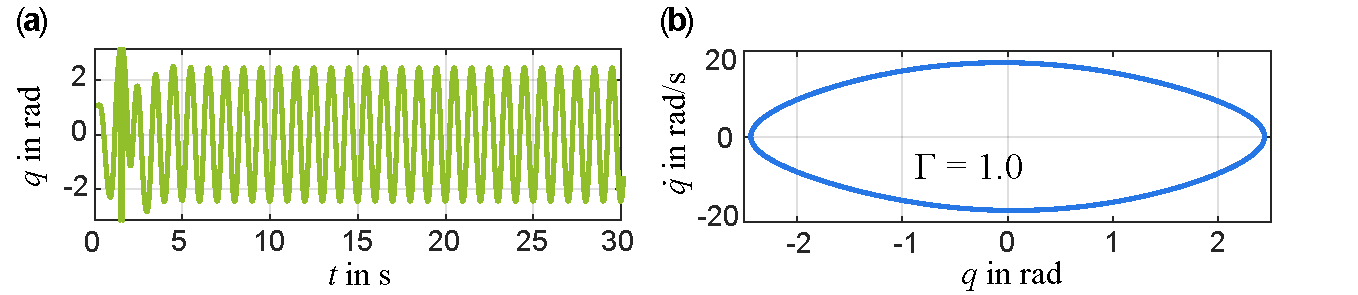
\includegraphics[width=\textwidth]{NLOgamma100.pdf}%
\caption[Verhalten des getriebenen nichtlinearen Oszillators f�r $\Gamma=1.0$.]{\fa Auslenkung des getriebenen nichtlinearen Oszillators f�r $\Gamma=1.0$. \fb Der Phasenraum ergibt eine geschlossene Kurve, der Poincar�-Plot einen Punkt (nicht gezeigt). Die weiteren Parameter: $\omega_\text{A} = 2\pi$, $\omega_0 = 1.25 \omega_\text{A}$ und $\gamma = \omega_0/5$ (\mscr{} \mlbewref{NLOszillator01.m}).}
\label{abb:bew_Chaos01}
\end{figure}

\begin{figure}
\begin{minipage}{\textwidth}
\leftfigure{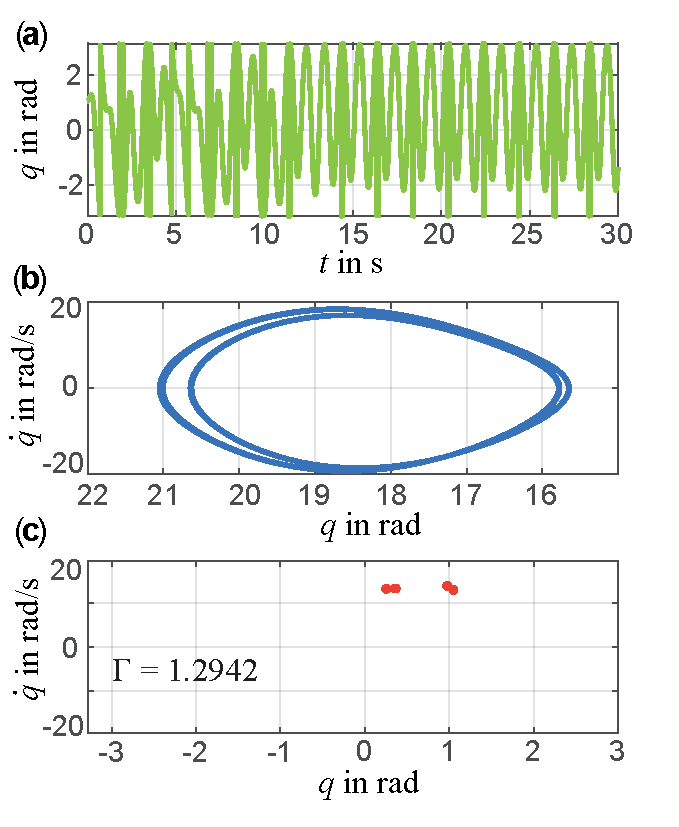
\includegraphics[width=0.5\textwidth]{NLOgamma12942.pdf}}%
\hspace{\fill}
\rightfigure{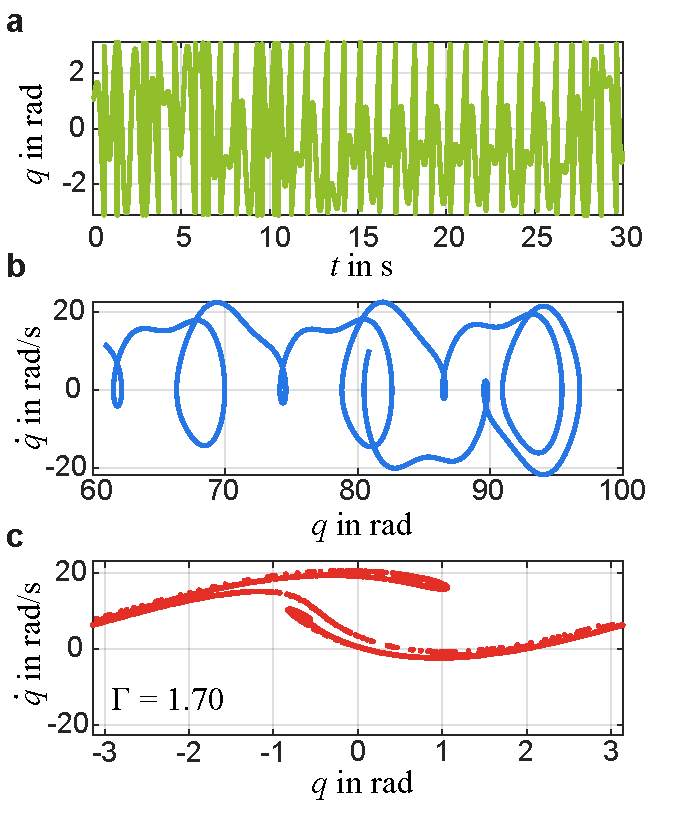
\includegraphics[width=0.5\textwidth]{NLOgamma170.pdf}}
\leftcaption[Verhalten des getriebenen nichtlinearen Oszillators f�r $\Gamma=1.2942$.]{\fa Auslenkung des getriebenen nichtlinearen Oszillators f�r $\Gamma=1.2942$. \fb Der Phasenraum ergibt vier ann�hernd geschlossene Kurven. \fc Der Poincar�-Plot zeigt vier Punkte. Die weiteren Parameter: $\omega_\text{A} = 2\pi\SI{}{\per\s}$, $\omega_0 = 1.25 \omega_\text{A}$ und $\gamma = \omega_0/5$ (\mscr{} \mlbewref{NLOszillator01.m}).}\label{abb:bew_Chaos02}
\rightcaption[Verhalten des getriebenen nichtlinearen Oszillators f�r $\Gamma=1.7$.]{\fa Auslenkung des getriebenen nichtlinearen Oszillators f�r $\Gamma=1.7$. \fb Der Phasenraum ergibt keine geschlossenen Kurven mehr, \fc Poincar�-Plot zeigt den sogenannten seltsamen Attraktor \textit{(Strange Attractor)}.}\label{abb:bew_Chaos03}
\end{minipage}
\end{figure}

Wir wollen jetzt aber noch der Frage nachgehen, wie man erkennen kann, ob bei gegebenen Parametern ein System chaotisches Verhalten zeigt.
Dazu kann man den sogenannten \index{Ljapunow-Exponent|textbf}Ljapunow-Exponenten\footnote{Alexander Michailowitsch Ljapunow\indexp{Ljapunow, Alexander Michailowitsch} (1857--1918) war ein russischer Mathematiker und Physiker, der vor allem auf dem Gebiet der Differentialgleichungen und der Stabilit�t dynamischer Systeme arbeitete.} verwenden, der ein Ma� f�r die Empfindlichkeit des nichtlinearen Systems f�r die Varianz in den Anfangsbedingungen ist.
Ist $\delta_{q0}= q_{01}-q_{02}$ ein Ma� ist f�r eine kleine Abweichung der Anfangsbedingungen, dann wird der Ljapunow-Exponent $\lambda$ nach
\begin{align}
    \Delta_{qt}= q_1\lk t\rk - q_2\lk t\rk = \delta_{q0}\,\e^{\lambda\,t}  \label{eq:bew_Chaos02}
\end{align}
berechnet, worin $\Delta_{qt}$ die Differenz der L�sungen zu einer gro�en Zeit $t$ ist.
Ist $\lambda < 0$, so werden die L�sungen nach langer Zeit konvergieren, f�r $\lambda > 0$ entsprechend divergieren.

\begin{figure}
\begin{minipage}{\textwidth}
\leftfigure{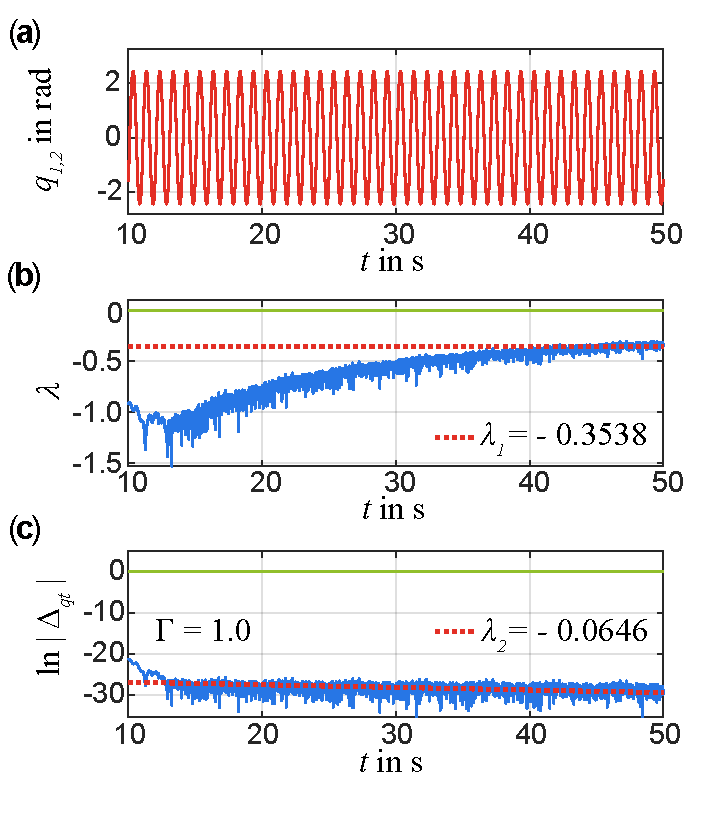
\includegraphics[width=0.5\textwidth]{NLOgammaLjapunow100.pdf}}%
\hspace{\fill}
\rightfigure{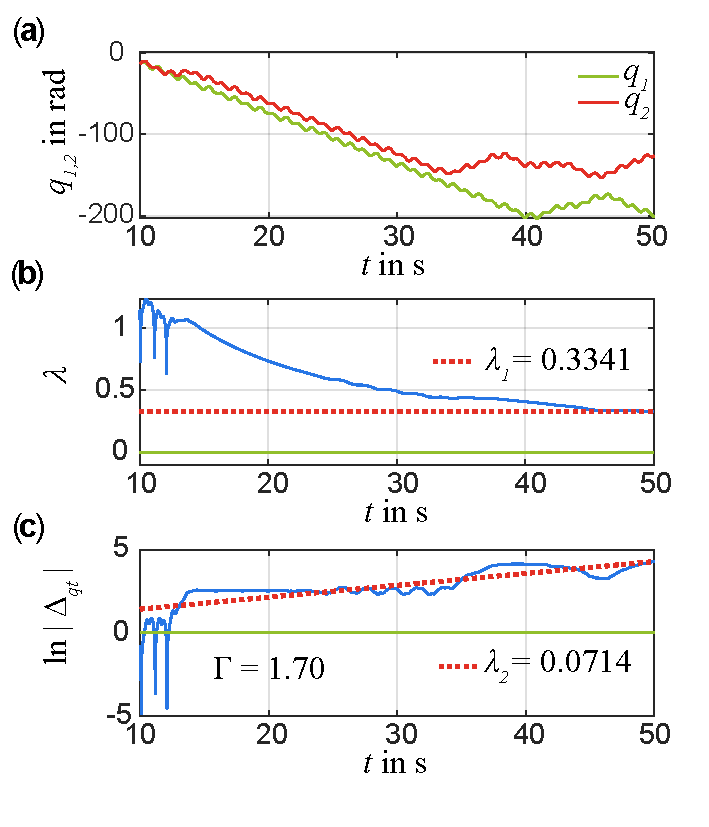
\includegraphics[width=0.5\textwidth]{NLOgammaLjapunow170.pdf}}
\leftcaption[Berechnung des Ljapunow-Exponenten f�r $\Gamma=1.0$.]{\fa Auslenkung und \fb\fc verschiedene Berechnungen des Ljapunow-Exponenten eines getriebenen nichtlinearen Oszillators f�r $\Gamma=1.0$. Die weiteren Parameter: $\omega_\text{A} = 2\pi\SI{}{\per\s}$, $\omega_0 = 1.25 \omega_\text{A}$ und $\gamma = \omega_0/5$ (\mscr{} \mlbewref{NLOszillator01.m}).  Der Ljapunow-Exponent $\lambda$ ist nach beiden Berechnungsmethoden kleiner als Null, das System ist stabil.}\label{abb:bew_Chaos04}
\rightcaption[Berechnung des Ljapunow-Exponenten f�r $\Gamma=1.7$.]{\fa Auslenkung und \fb\fc verschiedene Berechnungen des Ljapunow-Exponenten eines getriebenen nichtlinearen Oszillators f�r $\Gamma=1.7$. Der Ljapunow-Exponent $\lambda$ ist nach beiden Berechnungsmethoden gr��er als Null, das System zeigt chaotisches Verhalten.}\label{abb:bew_Chaos05}
\end{minipage}
\end{figure}

Wie bestimmt man nun den Ljapunow-Exponenten f�r ein nichtlineares dynamisches System wie den getriebenen nichtlinearen Oszillator?
Wir wollen dazu zwei N�herungsmethoden aufzeigen.
Wir berechnen im \mscr{} \mlbewref{NLOszillator02.m} wie f�r \figref{bew_Chaos01} und \figref{bew_Chaos03} die Trajektorien $q\lk t_0\rk$,
diesmal allerdings f�r zwei verschiedene Anfangsbedingungen,
die sich durch $q_{10}-q_{20} = 10^{-6}$ unterscheiden.
Ceteris paribus erhalten wir die Kurven in \figref{bew_Chaos04} und \figref{bew_Chaos05} f�r $q_1\lk t\rk$, $q_2\lk t\rk$ (Abb. a), $\Delta_{qt}$ (Abb. b) und $\ln\,\Delta_{qt}= \ln\,\delta_{q0}+\lambda\,t$ (Abb. c).
Offensichtlich ergibt sich f�r $\Gamma=1$ aus \figref{bew_Chaos04} ein $\lambda < 0$ und f�r $\Gamma = 1.7$ aus \figref{bew_Chaos05} ein $\lambda >0$.
Wir weisen darauf hin, dass diese numerischen Absch�tzungen des Ljapunow-Exponenten nur eine Indikation �ber das eventuell chaotische Verhalten des Systems geben.
In \cite{ Kuypers2012} wird gezeigt, wie man anhand einer Analyse der Differentialgleichung den Ljapunow-Exponenten gewinnen kann.

\subsection{Vermischtes zur Mechanik von Massepunkten und Massepunktsystemen}\label{kap:bew_mixed_mechanics}

\subsubsection{Streu- und Sto�prozesse}\index{Streuung} \label{kap:bew_scatter_problems}

\subparagraph{\textbf{Rutherford-Streuung}}\index{Streuung!Rutherford-}\index{Rutherford-Streuung}

In Kapitel Sto�- und Streuprozesse (\kap{bew_stoss}) haben wir die Formel \eqref{eq:bew_Streuung18} f�r den Wirkungsquerschnitt eines geladenen Teilchens im Coulomb-Feld  als Funktion des Streuwinkels $\vartheta'$ im Schwerpunktsystem (im Englischen oft \textit{Center of Mass}- oder CoM-System genannt)\index{Center of Mass} hergeleitet. Wir haben dabei das Streuzentrum (\zb einen Atomkern) im Laborsystem $\vec{\Sigma}_\text{L}$ als ruhend angenommen:
        \begin{align}
            \frac{\D \sigma'}{\D \Omega'} = \lk \frac{\alpha}{4E}\rk^2\,\frac{1}{\sin^4\,\lk\frac{\vartheta'}{2}\rk}\,. \label{eq:bew_Rutherford_review}
        \end{align}
Wir wollen nun den Wirkungsquerschnitt im Laborsystem berechnen und zwar f�r verschiedene Massenverh�ltnisse von gestreutem Teilchen und Streuzentrum. Wir wollen dabei auch untersuchen, welchen Fehler man macht, wenn man den R�cksto� auf das Streuzentrum nicht ber�cksichtigt. In Gl. \eqref{eq:bew_Rutherford_review} sind im Einzelnen: \\ \\
\begin{tabular}{ll}
   $\alpha = e^2\,Z_\text{Z}\,Z_\text{T}/(4\pi\epsilon_0) ~~~\text{mit}$& \\
	 &\\
   $\epsilon_0 = \SI{8.854e-12}{\ampere\second\per\volt\per\metre}$ &(Dielektrizit�tskonstante),\index{Dielektrizit�tskonstante}\\
   $ e = \SI{1.602e-19}{\ampere\second}$ &(Elementarladung),\index{Elementarladung} \\ 
   $Z_\text{Z} $ &(Kernladungszahl des Streuzentrums),\index{Kernladungszahl}  \\
   $Z_\text{T} $ &(Ladung des gestreuten Teilchens), \\
   $m_\text{Z} = 197 \, \uA $ &(Masse des Streuzentrums-Gold), \\
   $\uA = \SI{1.660539e-27}{\kg} $ &(atomare Masseneinheit),\index{Masseneinheit!atomare} \\
   $E $ & (Energie des Streuteilchens),\\
   $m_\text{eff}= m_\text{Z}\,m_\text{T}/(m_\text{Z} + m_\text{T})$ &(effektive Masse der beiden wechselwirkenden Teilchen). \\ \\
\end{tabular} \\ \\
Mit Gl. \eqref{eq:bew_Streuung7} hatten wir einen Zusammenhang zwischen dem Streuwinkel im Laborsystem $\vartheta_1$ und dem Streuwinkel $\vartheta'$ im Schwerpunktsystem hergeleitet. Wir wollen hier zur besseren Unterscheidung der beiden Winkel den Streuwinkel im Laborsystem mit $\psi = \vartheta_1$ bezeichnen. Bildet man die Ableitung $\D \psi / \D \vartheta'$ von 
\begin{align}
  \psi  = \arctan \lk \frac{\sin\vartheta'}{\cos\vartheta' + \frac{m_T}{m_Z}}  \rk \label{eq:bew_Rutherford00}
\end{align}
 und setzt diese gleich Null, erh�lt man im Fall, dass das Streuzentrum schwerer ist als das gestreute Teilchen (${m_T} \geq {m_Z}$) den maximalen Streuwinkel im Laborsystem zu
\begin{align}
	\tan \psi_\text{max} = \frac{m_\text{T}/m_\text{Z}}{\sqrt{1-\lk m_\text{T}/m_\text{Z} \rk^2}} \,~ \rightarrow ~~ \psi_\text{max} = \arcsin{\frac{m_\text{T}}{m_\text{Z}}}\,. \label{eq:bew_Rutherford01}
\end{align}
F�r ${m_T} = {m_Z}$  betr�gt dieser $90\degree$, es gibt in diesem Fall also keine R�ckstreuung. \\
Wir wollen nun den differentiellen Wirkungsquerschnitt als Funktion des im Laborsystem experimentell bestimmbaren Streuwinkels $\psi$ berechnen. Dazu halten wir fest, dass der Wirkungsquerschnitt im CoM- und im Laborsystem gleich sein muss, was gleichbedeutend ist mit
\begin{align}
      \frac{\D \sigma}{\D \Omega} 2\pi\,\sin\psi \,\D \psi  \stackrel{!}{=} \frac{\D \sigma'}{\D \Omega'} 2\pi\,\sin\vartheta' \,\D \vartheta'\,. \label{eq:bew_Rutherford02}
\end{align}
Hieraus folgt
\begin{align}
	%\frac{\D \sigma(\psi)}{\D \Omega} &= \frac{\D \Omega}{\D \Omega'} \, \frac{\D \sigma(\theta')}{\D \Omega'} \nonumber \\
	\frac{\D \sigma(\psi)}{\D \Omega} &= \frac{\sin\vartheta'(\psi)}{\sin\psi} \,\frac{\D \vartheta'(\psi)}{\D\psi} \frac{\D \sigma(\vartheta')}{\D \Omega'}\,. \label{eq:bew_Rutherford03}
\end{align}
Gl. \eqref{eq:bew_Rutherford03} ergibt relativ komplexe Zusammenh�nge zwischen den beiden differentiellen Streuquerschnitten, wir k�nnen hier vorteilhaft mit \matlab{} numerisch rechnen. Eine einfache analytische L�sung ergibt sich f�r den Spezialfall, bei dem Streuzentrum und gestreutes Teilchen dieselbe Masse haben. Dann ist nach \eqref{eq:bew_Streuung7} $\psi = \vartheta'/2$ und aus \eqref{eq:bew_Rutherford03} folgt
\[\frac{\D \sigma(\psi)}{\D \Omega} = 4\, \cos\psi \frac{\D \sigma(\vartheta')}{\D\Omega'} \,.\]
Im \mscr{} \mlbewref{Rutherford.m} haben wir verschiedene F�lle untersucht: 
\begin{itemize}
\item \textit{Fall 1:\, Gold $_{197}^{79}$Au- und Silber $_{109}^{47}$Ag-Teilchen auf Goldfolie } \\ \\
\begin{tabular}{ll} 
Schwerpunktsystem & Laborsystem mit R�cksto� \\ \\
$m_\text{T} = 197 \uA \,,~m_\text{Z} = 197 \uA,~ E = \SI{1e7}{\electronvolt}~~$& $E_\text{L} = {m_\text{Z} + m_\text{T}}/{m_\text{Z}}\, E = 2 E$\\
$m_\text{T} = 109 \uA \,,~m_\text{Z} = 197 \uA,~ E = \SI{1e6}{\electronvolt}~~$& $E_\text{L} = {m_\text{Z} + m_\text{T}}/{m_\text{Z}}\, E = 1.55 E$  
\end{tabular} \\ \\
\item \textit{Fall 2:\, $_2^4$He-($\alpha$)-Teilchen\index{Alpha-Teilchen@$\alpha$-Teilchen}\index{Alpha-Teilchen} auf Gold- und Silberfolie} \\ \\
\begin{tabular}{ll} 
Schwerpunktsystem & Laborsystem mit R�cksto� \\ \\
$m_\text{T} = 4 \uA \,,~m_\text{Z} = 197 \uA, ~ E = \SI{5e5}{\electronvolt}~~$ & $E_\text{L} = {m_\text{Z} + m_\text{T}}/{m_\text{Z}}\, E = 1.02 E$\\
$m_\text{T} = 4 \uA \,,~m_\text{Z} = 109 \uA, ~ E = \SI{5e5}{\electronvolt}~~$ & $E_\text{L} = {m_\text{Z} + m_\text{T}}/{m_\text{Z}}\, E = 1.04 E$ 
\end{tabular} \\ 
\end{itemize}
Das Ergebnis der Rechnungen ist in \figref{bew_Rutherford01} gezeigt.
\begin{figure}
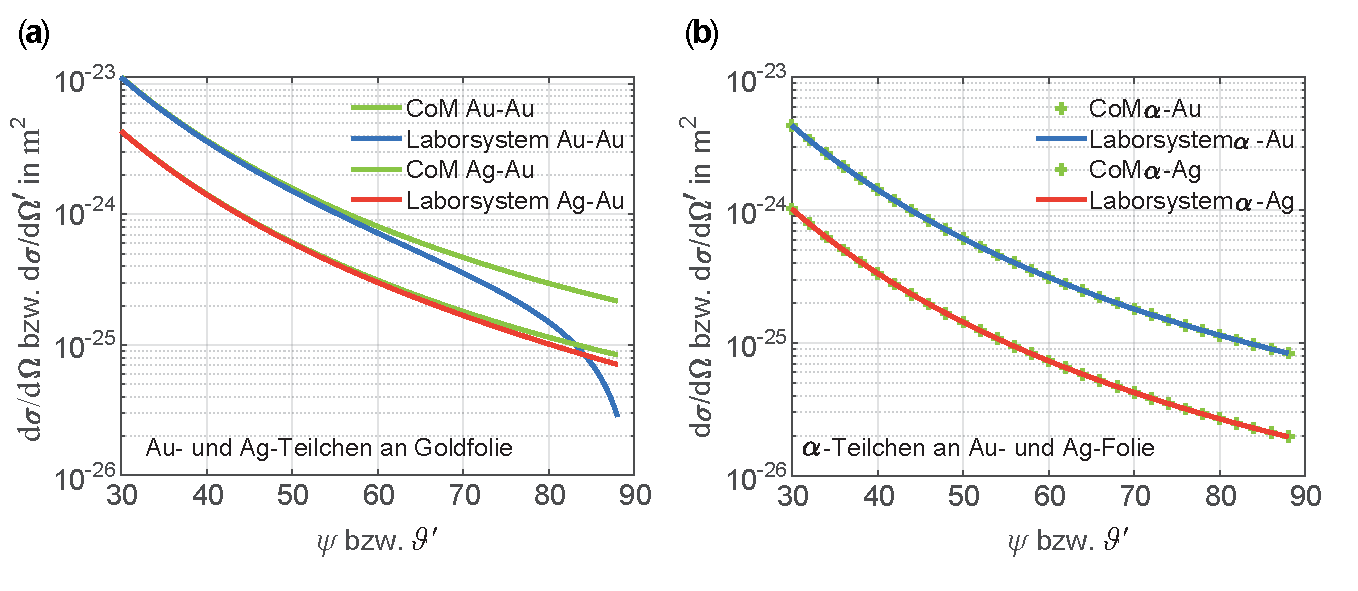
\includegraphics[width=\textwidth]{Rutherford01.pdf}%
\caption[Rutherford-Streuung von Gold- und Silberatomen.]{Rutherford-Streuung von \fa Gold- \bzw Silberatomen, sowie \fb $\alpha$-Teilchen jeweils an einer Goldfolie. CoM steht f�r Betrachtung im Schwerpunktsystem (\textit{Center of Mass}).}
\label{abb:bew_Rutherford01}
\end{figure}

Im Vergleich der Bilder a) und b) erkennt man sehr sch�n,
dass im Experiment von 1913 \cite{Geiger1913} zur Rutherford-Streuung
die Benutzung der Formel f�r das CoM System \eqref{eq:bew_Streuung19} gerechtfertigt war,
da $m_\text{T} \ll m_\text{Z}$.
Bei vergleichbaren Massen von Streuzentrum und Streuteilchen
wie \zb im Fall des Beschusses der Goldfolie mit hochenergetischen Gold- oder Silberteilchen
ist die N�herung aber nicht mehr gerechtfertigt. \\
In \probref{bew_Rutherford} und in den \mscren \mlbewref{RutherfordAlpha.m} \bzw \mlbewref{RutherfordAg.m} zeigen wir, wie man das Streuproblem durch numerische Integration der Bewegungsgleichungen f�r verschiedene Einfallstrajektorien (Sto�parameter $b$) simulieren und l�sen kann.

\subparagraph{\textbf{Asteroidenbahnen}}

Wir wollen noch darauf hinweisen, dass auch die Bewegung nicht geschlossener Asteroidenbahnen (oder Bahnen anderer Himmelsk�rper) als Streuproblem nach dem Rutherford-Modell betrachtet werden kann, da das Gravitationspotential ja dieselbe Struktur hat wie das Coulomb-Potential. Man setzt einfach in \eqref{eq:bew_Rutherford_review} $\alpha = G\,m_\text{A}\,m_\text{E}$ (mit $m_\text{A}$ als Masse des Asteroiden und $,m_\text{E}$ als Masse der Erde) und kann dann alle Formeln entsprechend verwenden. \\
Wir wollen vereinfachend annehmen, dass sich die beiden wechselwirkenden K�rper in der $x$-$y$-Ebene bewegen, die gleichzeitig die Ebene der Mondbahn und der Erde sein soll. Das ist 
ein Zweik�rperproblem Erde-Asteroid (\figref{bew_asteroid}) mit folgenden (etwas willk�rlich) angenommenen Parametern.\footnote{So ganz willk�rlich sind die Parameter nicht. Am 15.\ Februar 2013 kam der Asteroid 367943 Duende der Erde bis auf \SI{27.599}{\kilo\metre} nahe, was innerhalb der Umlaufbahn der geostation�ren Satelliten lag. Der Asteroid war sogar mit blo�em Auge zu erkennen (\url{https://www.nasa.gov/topics/solarsystem/features/asteroidflyby.html}\, Durch Einfl�sse von Erde und Mond wurde seine Bahn um die Sonne signifikant ver�ndert. So verk�rzte sich \zb seine Umlaufperiode um die Sonne von 336 auf 317 Tage.\cite{JPL2020}}:
\begin{align*}
    v_\infty &=  \SI{4}{\km\per\s} && \text{Geschwindigkeit relativ zur Erde vor der Begegnung}\,, \\
    b &= \SI{25000}{\km} && \text{Sto�parameter}, \\
    \epsilon &= 1.004 && \text{Exzentrizit�t und} \\
    \varphi &= \arccos \lk -\frac{1}{\epsilon}\rk \approx 175\degree && \text{�ffnungswinkel, sowie} \\
    r_\text{min} & \approx \SI{10700}{\km} \,.
\end{align*}

\begin{figure}
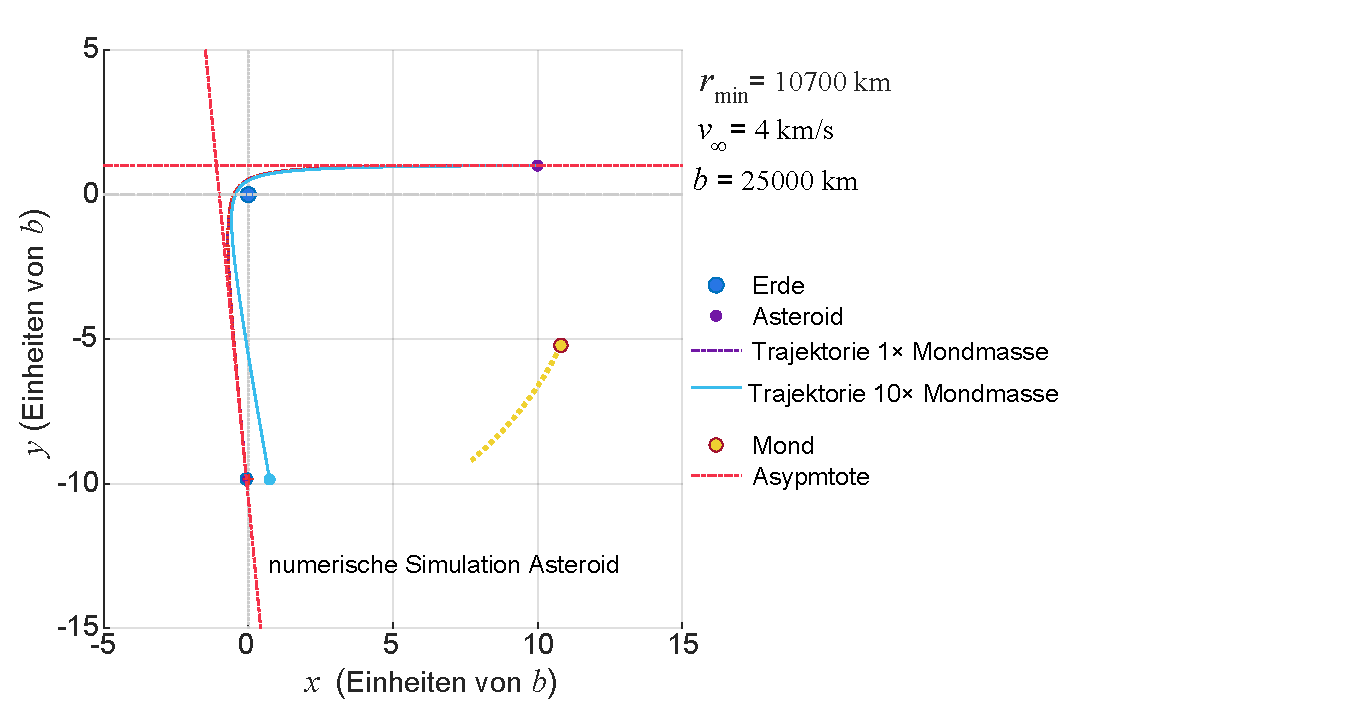
\includegraphics[width=\textwidth]{Asteroid.pdf}%
\caption[Streuung eines Asteroiden im Gravitationsfeld von Erde und Mond.]{Streuung eines Asteroiden im Gravitationsfeld von Erde und Mond (vereinfachte Annahmen). Im Bild wird die Streuung durch den Mond in sogenannter Oppositionsstellung zum Asteroiden und im Vergleich dazu bei Annahme eines Mondes mit zehnfach gr��erer Masse gezeigt.}
\label{abb:bew_asteroid}
\end{figure}

Wenn wir die Erde als ruhend in (0,0) annehmen, wird das Ganze 
mit $m_\text{E} \gg m_\text{A}$ dann
ein einfaches Streuproblem.
Wir k�nnten die L�sung dieses Streuproblems entweder nach der Hyperbell�sung von \kapitel{bew_ZKP_NZKF} oder auch als Streuproblem nach \kap{bew_stoss} darstellen:
Wir wollen hier aber die Trajektorie des Asteroiden numerisch
berechnen und dabei untersuchen, was passiert, wenn 
wir den Mond in unsere Betrachtungen einschlie�en.
Wir nehmen vereinfachend an, dass dieser sich mit konstanter
Umlaufgeschwindigkeit auf einer Kreisbahn um die Erde bewegt
und die Position der Erde sich nicht ver�ndert
(was nicht ganz korrekt ist, siehe Himmelsmechanik im Band II, Kapitel 3).
Der Asteroid bewegt sich dann in einem zeitlich ver�nderlichen
Gravitationspotential, seine Bewegungsgleichung lautet%
\footnote{Man kann das Problem auch als Streuung an einem
zeitlich ver�nderlichen \bzw bewegten Streuzentrum verstehen.}
\begin{align}
    m_\text{A}\,\ddot{\vec{ r}}_\text{A} = - m_\text{A}\,G\,\lek \frac{ m_\text{E}}{|\vec{r}_\text{A}|^2} + \frac{ m_\text{M}}{|\vec{r}_\text{A}-\vec{r}_\text{M}|^2}\rek ~~ \label{eq:bew_asteroid01a}\\
		\text{mit} ~~ \vec{r}_\text{M} = 		\begin{pmatrix} x_\text{M}\\ y_\text{M} \end{pmatrix} =
  \begin{pmatrix}
      R_\text{ME}\,\cos\omega_\text{M}t + \varphi_0\\
      R_\text{ME}\,\sin\omega_\text{M}t + \varphi_0
  \end{pmatrix} \,. \label{eq:bew_asteroid01b}
\end{align}
Wir wollen Gl. \eqref{eq:bew_asteroid01a} numerisch integrieren und erhalten mit $\vec{r}_\text{A} = \begin{Bmatrix} x\\ y \end{Bmatrix}$
\begin{align}
    \ddot{\vec{x}} &= \begin{pmatrix} \ddot{x} \\ \ddot{y} \end{pmatrix} = - \frac{G\,m_\text{E}} {\lk x^2+y^2 \rk^{3/2}} \begin{Bmatrix} x\\ y \end{Bmatrix} -\frac{G\,m_\text{M}}{\lk x-x_\text{M}\rk^2 + \lk y-y_\text{M}\rk^2} \begin{Bmatrix} x-x_\text{M}\\ y-y_\text{M} \end{Bmatrix} \\ \label{eq:bew_asteroid02}
    & \text{mit} \nonumber \\
    R_\text{ME} &= \SI{384000}{\km}~~\text{und}~~ \omega_\text{M}  = \sqrt{\frac{G\,\lk m_\text{E} + m_\text{M} \rk}{R_\text{ME}^3}} \approx \SI{2.6e-06}{\per\second}\,.
\end{align}

Die numerische Integration von \eqref{eq:bew_asteroid02} haben wir im \mscr{} \mlbewref{Asteroid.m} ausgef�hrt und das Ergebnis ist in \figref{bew_asteroid} zu sehen: Es zeigt, dass der Mond einen geringen, aber doch messbaren Einfluss auf die Streuung und damit die Bahn des Asteroiden hatte. In ung�nstigerer Konstellation k�nnte der Mond durchaus einen ansonsten an der Erde vorbeifliegenden Asteroiden so abenken, dass er auf der Erde aufschl�gt. 


\subsubsection{Fallschirmsprung} \index{Fall!freier}\index{Fallschirmsprung}\label{kap:bew_parachute}

Das Fallschirmspringen hat eine erstaunlich lange Tradition:
Schon im alten China sprangen im 14.\ Jahrhundert Menschen mit Fallschirmen von T�rmen.
In Europa hat Leonardo da Vinci%
\footnote{Leonardo da Vinci (1452--1519) war eines der gro�en Universalgenies der Renaissance,
er war bildender K�nstler, Architekt, Anatom, Ingenieur und Naturphilosoph.
Besonders seine vielen mechanischen Konstruktionen, von denen aber nicht alle funktionierten,
haben die Menschen begeistert.}
in heute noch erhaltenen Originalzeichnungen Fallschirmspringer festgehalten
(\url{http://www.museoscienza.org}). \\
Am 14.~Oktober~2012 sprang der �sterreicher Felix Baumgartner
aus $\SI{39}{\km}$ H�he aus einem Ballon und erreichte im freien
Fall eine Maximalgeschwindigkeit von $\SI{1342}{\km\per\hour}$.
Er war damit der erste Mensch, der ohne zus�tzlichen Antrieb
die sogenannte Schallmauer durchbrach.%
\footnote{Ohne zus�tzlichen Antrieb ist wohl auch etwas untertrieben,
immerhin kostete die Unternehmung ca.\ 50 Millionen USD.}
Wir wollen diesen Rekord zum Anlass nehmen und die Dynamik des freien Falls aus gro�er H�he untersuchen.
Dabei wollen wir uns auch der Frage widmen, auf welche H�he man mindestens steigen muss, um im freien Fall �berschallgeschwindigkeit zu erreichen. 
Wir modellieren den Sprung von Baumgartner in vier Phasen \cite{Corvo2019}:
\begin{itemize}
    \item [A] -- freier Fall (in gro�er H�he)
    \item [B] -- freier Fall in mittlerer H�he und Vorbereitung f�r Schirm�ffnung
    \item [C] -- Schirm�ffnung 
    \item [D] -- finale Phase mit Schirm
\end{itemize}

\subparagraph{\textbf{Phase A -- Absprung bis Schirm�ffnung}}

Die Bewegungsgleichung f�r die H�he $z$ �ber der Erdoberfl�che in Phase A lautet 
        \begin{align}
            \ddot{z} = -g + \eta\,{\dot{z}}^2 = -g + \hat{\eta}_0\,\rho(z)\,{\dot{z}}^2 = -g + \hat{\eta}_0\,\varrho_0\,\e^{-\kappa\,z}\,{\dot{z}}^2 = -g + \eta_0\,\e^{-\kappa\,z}\,{\dot{z}}^2\,. \label{eq:bew_skydive01}
        \end{align}
Hierin ist $\eta$ der Widerstandskoeffizient, dessen Abh�ngigkeit von $z$ wir hier mithilfe der \emph{barometrischen H�henformel}\glslink{baroHoeheBew} (siehe \probref{kontmech_BarometrischeHoehenformel}) modelliert haben.\index{H�henformel!barometrische}
Prinzipiell k�nnte der Widerstandskoeffizient auch von der Geschwindigkeit abh�ngen, aber dies wollen wir hier der Einfachheit halber vernachl�ssigen.
Wir verwenden die Werte
 \begin{align*}
    \varrho_0 &=\SI{1.225}{\kg\per\cubic\metre}\,,~~~\kappa = \frac{\tilde{M}_\text{L}\,g}{k_\text{B}\,T}\,,~~~ \hat{\eta}_0 = \frac{1}{2\,m}\,A\,c_\text{W}\,,
  \end{align*}
worin $\tilde{M}_\text{L} = \SI{28.9e-3}{\kg\per\mole}$ die molare Masse der Luft, $T$ die absolute Temperatur und $k_\text{B} = \SI{1.381e-23}{\J\per\K\per\mole}$ die Boltzmann-Konstante sind. 
Offensichtlich ist der Widerstandskoeffizient wegen \eqref{eq:bew_skydive01} in gro�en H�hen deutlich geringer.%
\footnote{Da $\kappa$ von der Temperatur und diese ihrerseits von der H�he abh�ngt, gilt streng genommen $\kappa(z)\approx \frac{1}{T(z)}$.
Wir wollen aber zun�chst $\kappa = \con$ mit einer mittleren Temperatur annehmen.} \\
Im freien Fall in einem Medium mit Reibung wird eine Endgeschwindigkeit $v_\text{final}$ erreicht.
Wir nehmen an, dass die Schwerebeschleunigung konstant ist, \dh $g\lk z\rk = g = \con$ und erhalten
\begin{align}
    v_\text{final}\lk z\rk = \sqrt{\frac{2m\,g}{A\,c_\text{W}\,\varrho \lk z\rk}}\,. \label{eq:bew_skydive03}
\end{align}
In der N�he des Erdbodens gilt
$v_\text{final}\lk 0\rk = v_\text{final, 0} = \sqrt{\frac{2m\,g}{\varrho_0\,A\,c_\text{W}}}$, sodass 
\begin{align}
    \frac{v_\text{final}\lk z\rk}{v_\text{final, 0}} = \sqrt{\frac{\varrho_0}{\varrho\lk z\rk}} \label{eq:bew_skydive04}
\end{align}
ist. 
Wir wollen nun wissen, von welcher H�he aus man mindestens springen muss, um die Schallgeschwindigkeit $v_\text{S}$\index{Schallgeschwindigkeit} zu erreichen.
Wir setzen also $v_\text{final}\lk z\rk = v_\text{S}$ und erhalten aus \eqref{eq:bew_skydive04} und \eqref{eq:bew_skydive03} f�r die minimale atmosph�rische H�he, in der durch freien Fall Schallgeschwindigkeit erreicht werden kann
    \begin{align}
        z_\text{min}' = 2\,\ln\lk \frac{v_\text{S}}{v_\text{final, 0}}\rk \,\frac{1}{\kappa}\,.\label{eq:bew_skydive04a}
    \end{align}
Dazu muss man mindestens noch die Fallstrecke 
    \begin{align*}
        z_\text{fall} = \frac{1}{2}\,\frac{{v_\text{S}}^2}{g} 
    \end{align*}
addieren, die (bei Vernachl�ssigung der Reibung) durchlaufen werden muss,
um die Schallgeschwindigkeit%
\footnote{Auch die Schallgeschwindigkeit h�ngt von $v_\text{S}$ ab,
sodass \eqref{eq:bew_skydive04a} eigentlich eine transzendente Gleichung wird:
$\ln v_\text{S}(z_\text{min}') = \ln v_\text{final,0}+(1/2)\,\kappa\,z_\text{min}'$.}
zu erreichen, sodass wir schlie�lich
        \begin{align}
            z_\text{min} \geq {z_\text{min}}'+z_\text{fall} \approx \SI{30}{\km}\label{eq:bew_skydive05}
        \end{align}
erhalten.
Wir haben dabei $v_\text{final, 0} \approx \SI{80}{\metre\per\second}$, $\kappa \approx \SI{0.125}{\per\km}$ und $v_\text{S} \approx \SI{330}{\metre\per\second}$ angenommen.
Man sieht also, dass tats�chlich eine sehr gro�e Anfangsh�he von mehr als $\SI{30}{\km}$ notwendig ist, um Schallgeschwindigkeit im freien Fall zu erreichen. \\
Wir wollen jetzt noch Bewegungsgleichung \eqref{eq:bew_skydive01} l�sen.
Durch die Substitutionen 
	\[v^2 = \dot{z}^2 = u ~~~\text{und}~~~\ddot{z} = \frac{\D z}{\D t}\frac{\D \dot{z}}{\D z} = v\,\frac{\D v}{\D z}
	\]
k�nnen wir diese auf die Form 
\begin{align}
    \frac{\D u}{\D z}-2\eta_0\,e^{-\kappa\,z}\,u =-2g \label{eq:bew_skydive06}
\end{align}
bringen. 
Das entspricht einer DGL des Typs
\begin{align}
    \frac{\D u}{\D z}+A\lk z\rk\, u = B\lk z\rk, \label{eq:bew_skydive07}
\end{align}
deren allgemeine L�sung durch
\begin{align}
    u\lk z\rk = \frac{\int B\lk z'\rk\,\text{exp}\lek\int A\lk z''\rk\,\D z''\rek\,\D z'}{\text{exp}\lek\int A\lk z' \rk \D z'\rek} 
    \label{eq:bew_skydive08}
\end{align}
gegeben ist \cite{Andrews2003, Felder2016}.
Mit der Substitution $q = \frac{2\eta_0}{\kappa}\,\text{exp}\lk -\kappa z\rk$ kann \eqref{eq:bew_skydive08} unter Nutzung des sogenannten \textit{exponentiellen Integrals}\index{Integral!exponentielles} \cite{Gradshteyn1980}
\begin{align*}
    \textbf{Ei}\lk q\rk = \int\limits_{-\infty}^q \,\frac{\text{exp}\lk z'\rk}{z'} \,\D z'
\end{align*}
in die L�sung 
\begin{align}
    v\lk q\lk z\rk\rk = \sqrt{u} = \sqrt{\frac{2g}{\kappa}\,e^{-q}\,\lek \textbf{Ei}\lk q\rk + C\rek}  \label{eq:bew_skydive08A}
\end{align}
gebracht werden, worin $C$ eine Integrationskonstante ist, die durch $v(0)=v_0$ bei $z(0)=z_0$ festgelegt wird. 
Bei einer Anfangsgeschwindigkeit von $v_0=0$ gilt
	\[ C = - \textbf{Ei}\lk q(z_0) \rk = - \textbf{Ei}\lk \frac{2\eta_0}{\kappa}\,e^{-\kappa\,z}\rk \,.
\]

\begin{figure}
\begin{minipage}{\textwidth}
\leftfigure{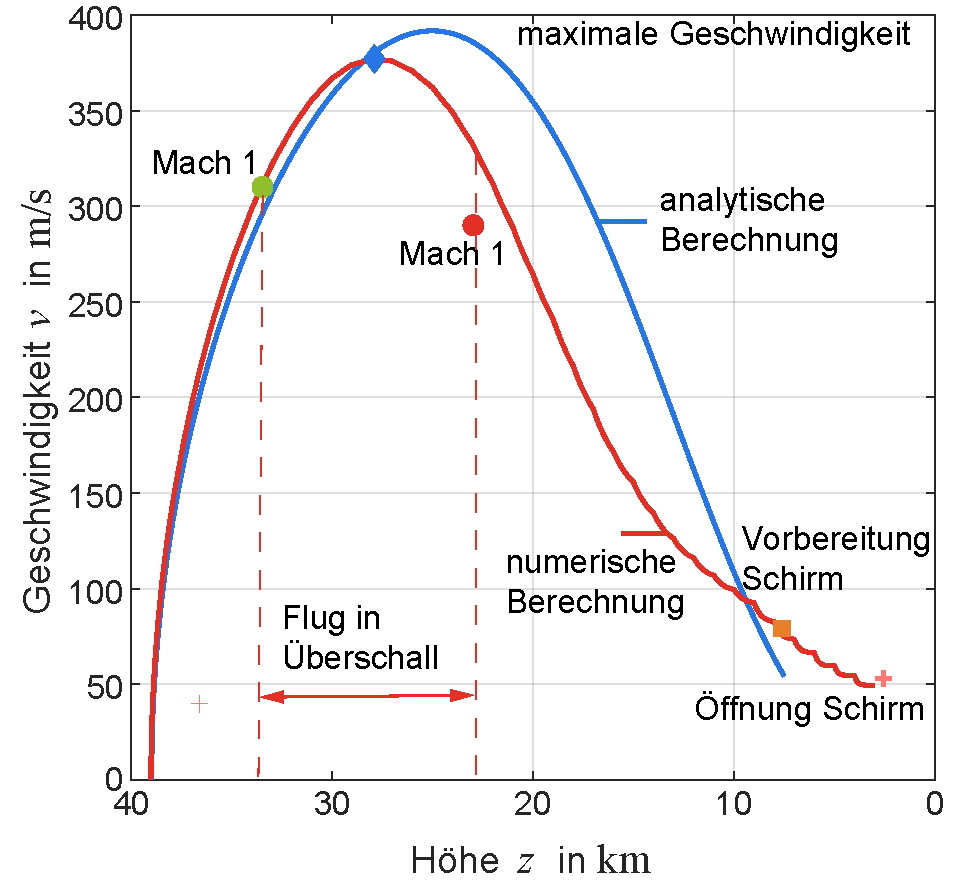
\includegraphics[width=0.5\textwidth]{BaumgartnerFall.pdf}}%
\hspace{\fill}
\rightfigure{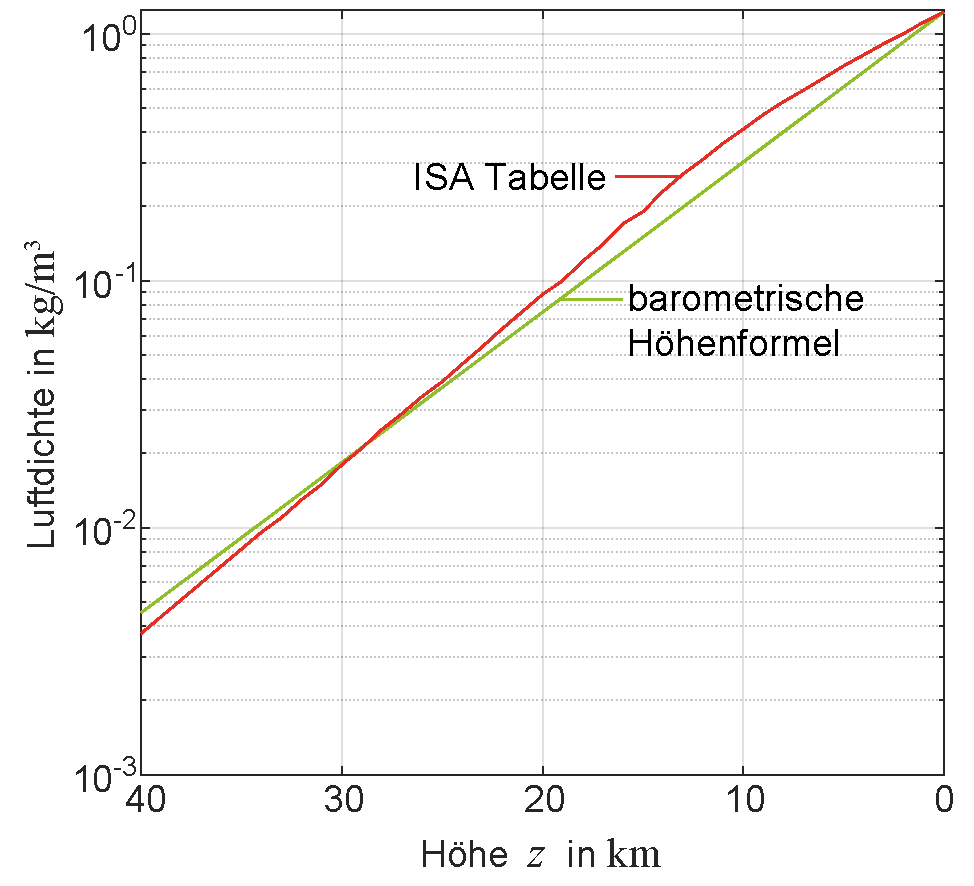
\includegraphics[width=0.5\textwidth]{BaromHoehe.pdf}}
\leftcaption[Fall mit �berschallgeschwindigkeit von Felix Baumgartner.]{Fall mit �berschallgeschwindigkeit von Felix Baumgartner \cite{Corvo2019}. Geschwindigkeit-H�henkurve. Dargestellt sind die Messwerte (einzelne Punkte), die N�herungsberechnung nach der barometrischen H�henformel und die numerische Berechnung nach den tabellierten Werten. Mach 1 bedeutet Erreichen \bzw Unterschreiten der Schallgeschwindigkeit $v_\text{s}$.}\label{abb:bew_BaumgartnerFall}
\rightcaption[Dichteabh�ngigkeit der Atmosph�re nach barometrischer H�henformel.]{Dichteabh�ngigkeit der Atmosph�re nach der barometrischen H�henformel und nach der Standardtabelle \cite{ISA1976}.}\label{abb:bew_BaromHoehe}
\end{minipage}
\end{figure}

In \figref{bew_BaumgartnerFall} haben wir L�sung \eqref{eq:bew_skydive08A} dargestellt.
Wir haben dabei den Wert f�r die Starth�he $z_0 = \SI{38969}{\metre}$
aus \cite{Corvo2019} �bernommen und f�r $\kappa$ einen Mittelwert von
$\kappa \approx \SI{1.4e-4}{}$ als Fit an die barometrische H�henformel angenommen.
Wie wir im Vergleich zu den experimentellen Werten sehen, gibt es eine gute, aber keine perfekte �bereinstimmung (siehe auch \cite{Corvo2019}).
In einigen H�henbereichen gibt es gr��ere Abweichungen.
Neben der N�herung, die wir mit der barometrischen H�henformel gemacht haben,
muss man auch davon ausgehen, dass der $c_\text{w}$-Wert
nicht �ber den gesamten Fallbereich konstant ist, zum einen da der Springer
zu Beginn sicher die senkrechte Lage (Kopf nach unten) eingenommen hat,
um auf Geschwindigkeit zu kommen. Ab ca.~$\SI{10000}{\metre}$ H�he wird er aber
eher die horizontale Lage (Bauch nach unten) einnehmen, um den Fall abzubremsen,
bevor der Schirm ge�ffnet wird.
Ferner ist der $c_\text{w}$-Wert auch im Bereich von Geschwindigkeiten, die im Ultraschalbereich liegen, deutlich unterschiedlich,
siehe \autoref{chap:kontmech}.\\
Wir wollen deswegen die DGL \eqref{eq:bew_skydive01} st�ckweise integrieren, wobei wir die Werte f�r $\varrho\lk z \rk$ aus der US Standard Atmosphere Table \cite{ISA1976} benutzen (siehe \figref{bew_BaromHoehe}). 
Tab.\ \ref{tab:bew_BaumgartnerFall}  und auch die so berechnete Kurve $v(z)$ in \figref{bew_BaumgartnerFall} zeigen eine deutlich bessere �bereinstimmung mit den experimentellen Werten.

\begin{table}[h!]
  \centering
  \begin{tabular}{|C{20mm}|C{15mm}|C{15mm}|C{15mm}|C{15mm}|C{15mm}|C{15mm}|}
  \hline
  \rule{0pt}{3pt}& & & & & &   \\
    & H�he \linebreak exper.\linebreak\linebreak  $\SI{}{\metre}$  & $v$ \linebreak exper.\linebreak \linebreak $\SI{}{\metre\per\second}$ & Zeit \linebreak exper.\linebreak \linebreak $\SI{}{\second}$ & H�he \linebreak Gl. \eqref{eq:bew_skydive08A} \linebreak\linebreak  $\SI{}{\metre}$  & H�he \linebreak Gl. \eqref{eq:bew_skydive01}\linebreak \linebreak  $\SI{}{\metre} $& Zeit \linebreak Gl. \eqref{eq:bew_skydive01} \linebreak \linebreak $\SI{}{\second}$\\
  \rule{0pt}{3pt}& & & & & &  \\
  \hline
  \rule{0pt}{3pt}& & & & & &  \\
  \rule{0pt}{6pt} ~Start   & $\SI{38969}{}$ & $\SI{0}{}$ & $\SI{0}{}$ & $\SI{0}{}$ & $\SI{0}{}$ &  $\SI{0}{}$  \\
  \rule{0pt}{6pt} ~Mach 1   & $\SI{33446}{}$ & $\SI{310}{}$ & $\SI{34}{}$ & $\SI{32669}{}$ & $\SI{33446}{}$ &  $\SI{33}{}$  \\
  \rule{0pt}{6pt} ~Max $v$   & $\SI{27883}{}$ & $\SI{377}{}$ & $\SI{50}{}$ & $\SI{25360}{}$ & $\SI{27883}{}$ &  $\SI{51}{}$  \\
  \rule{0pt}{6pt} ~Mach 1   & $\SI{22961}{}$ & $\SI{290}{}$ & $\SI{64}{}$ & $\SI{17200}{}$ & $\SI{21785}{}$ &  $\SI{69}{}$  \\
  \rule{0pt}{3pt}& & & & & &  \\
  \rule{0pt}{6pt} ~Schirmvorber. & $\SI{7619}{}$ & $\SI{79}{}$ & $\SI{180}{}$ & $\SI{7563}{}$ & $\SI{7438}{}$ &  $\SI{170}{}$  \\
  \rule{0pt}{6pt} ~Schirm�ffnung  & $\SI{2567}{}$ & $\SI{53}{}$ & $\SI{260}{}$ &  &  & \\
  \rule{0pt}{3pt}& & & & & &   \\
  \hline
  \end{tabular}
  \caption[Baumgartner Fall mit �berschallgeschwindigkeit.]{Baumgartner Fall mit �berschallgeschwindigkeit.} \label{tab:bew_BaumgartnerFall}
\end{table}

Mach 1 bedeutet Erreichen \bzw Unterschreiten der Schallgeschwindigkeit $v_\text{s}$, die wir aus \cite{ISA1976} f�r die entsprechende H�he entnommen haben.
Wir wollen jetzt noch kurz die Phase des �ffnens und der Landung mit realistischen Werten betrachten.\\

\subparagraph{\textbf{Phase B -- Landung mit Schirm}}

Der Schirm wird bei $z \approx \SI{2500}{\metre}$ ge�ffnet. Die Entfaltung des Schirms dauert ca.~$\SI{5}{\second}$ (angenommen), der Schirm erzeugt dabei eine Bremsbeschleunigung von bis ca.~$\SI{4}{\g}$, hat also in dieser Phase eine Reibungskraft von 
\begin{align*}
    F_\text{R}\lk z\rk = \frac{1}{2}\,c_\text{w}\,\varrho\lk z\rk\,A\,v^2\lk z\rk\,~~\text{mit}~~c_\text{w} = \SI{1.15}{}\,.
\end{align*}
Die Fl�che steigt in der �ffnungszeit kontinuierlich (n�herungsweise linear) im Laufe von $\SI{5}{\second}$
von ca.~$\SI{1}{\square\metre}$ auf $\SI{50}{\square\metre}$ an, $\varrho\lk z\rk$ k�nnen wir als w�hrenddessen konstant annehmen.
In dieser Phase ab $z = \SI{2500}{\metre}$ muss man also zun�chst eine kontinuierlich ansteigende Bremsverz�gerung
bis zur vollen �ffnung des Schirms in DGL \eqref{eq:bew_skydive01} annehmen.
Wir empfehlen die numerische Rechnung als \probref{bew_SkyDiver}.

Obwohl die Flugphase ab �ffnen des Schirms recht einfach erscheint,
ist deren Berechnung durchaus kritisch.
Kurz vor der �ffnung des Schirms hat der Springer eine Geschwindigkeit von $50 \ldots 60\, \SI{}{\metre\per\second}$, die man auch aus folgender Absch�tzung erh�lt:
        \begin{align*}
            \frac{1}{2}\,\varrho_\text{L}\,c_\text{w}\,A^{(0)}\,{{v_\infty}^{\lk 0\rk}}^2 &= m\,g ~~ \rightarrow ~~{v_\infty}^{\lk 0\rk} = \sqrt{\frac{m\,g}{\frac{1}{2}\,\varrho_\text{L}\,{c_\text{w}}^{\lk 0 \rk}\,A^{\lk 0 \rk}  }} \,.
        \end{align*}
Hierin sind die Werte ${c_\text{w}}^{\lk 0 \rk}$ und $A^{\lk 0 \rk} $ die Werte ohne Schirm, also ${c_\text{w}}^{\lk 0 \rk} \approx 0.3$ und $A^{\lk 0 \rk} \approx 2.53\,\SI{}{\square\metre} $.
Nach dem �ffnen des Schirms ist ${c_\text{w}}^{\lk \text{S} \rk} \approx 0.9 \ldots 1.2$ und $A^{\lk \text{S}\rk} \approx 50 \ldots 60\,\SI{}{\square\metre} $, \dh die Bremskraft steigt um das $60$- bis $80$-Fache an. Die Endgeschwindigkeit reduziert sich um
        \begin{align*}
            {v_\infty}^{\lk \text{S} \rk} \approx \sqrt{\frac{{c_\text{w}}^{\lk 0 \rk}\,A^{\lk 0 \rk}}{{c_\text{w}}^{\lk \text{S} \rk}\,A^{\lk \text{S} \rk}}}\,{v_\infty}^{\lk 0 \rk} \approx \sqrt{4\cdot20}\,{v_\infty}^{\lk 0 \rk} \approx 9\,{v_\infty}^{\lk 0 \rk}\,,
        \end{align*}
also ca.\ um das Neunfache, was in der Tat dann Landegeschwindigkeiten von ca.~$\SI{6}{\metre\per\second}$ ergibt, die in etwa einem Sprung von einer $\SI{1.5}{\metre}$ hohen Mauer entsprechen. 

Die Design-Problematik der �ffnungsphase besteht darin, eine �ffnungszeit des Fallschirms zu finden, die den sogenannten �ffnungsschock vermeidet. Man kann leicht ausrechnen, dass zur Vermeidung einer Belastung von mehr als $4\, g$ die �ffnungszeit $\Delta T$ des Fallschirms bei einer linearen �ffnungsfunktion von $c_\text{w}(t) \, A(t)$ mindestens $\SI{3}{\second}$ betragen muss. In der Realit�t wird man eher nichtlineare Zeitprofile w�hlen (am Anfang langsam, dann schnell) um die �ffnungszeit insgesamt zu minimieren. 

Zum Schluss geben wir der Vollst�ndigkeit halber noch die L�sung des freien Falls\index{Fall!freier} f�r niedrige H�hen, \dh bei konstanter Luftdichte an. In diesem Fall gilt:
        \begin{align}
            \ddot{z} &= -g+\beta\,\dot{z}^2\,,\\
            \frac{\D v_\text{z}}{\D t} = \dot{v}_\text{z} &= -g+\beta\,{v_\text{z}}^2~~\rightarrow ~~\frac{\D v}{-g+\beta\,v^2} &= \D t ~~~~ \text{mit} ~~~~ \beta = \frac{1}{2}\,\varrho_\text{L}\,c_\text{w}\,\frac{A}{m} \,. \label{eq:bew_Fall_exakt01}
        \end{align}
Integration \cite{Gradshteyn1980} ergibt: 
        \begin{align}
            t+C = \frac{1}{\sqrt{g\,\beta}}\frac{1}{2}\ln \lek \frac{1+v\frac{\beta}{g}}{1-v\frac{\beta}{g}} \rek= \frac{\artanh\sqrt{\frac{\beta}{g}\,v}}{\sqrt{g\,\beta}} \,. \label{eq:bew_Fall_exakt02}
        \end{align}
Mit $v\lk 0 \rk  = v_0$ und $\sqrt{g\,\beta} = g/v_\infty$ bestimmt man
        \begin{align}
            C &= \artanh \lk \frac{v_0}{v_\infty}\rk~~\rightarrow ~~v\lk t\rk &= -v_\infty\,\tanh \lk \frac{g\,t}{v_\infty}-\artanh \lk\frac{v_0}{v_\infty}\rk\rk\,. \label{eq:bew_Fall_exakt03}
        \end{align}
Nochmalige Integration \cite{Gradshteyn1980} ergibt
        \begin{align}
            z\lk t\rk = -\frac{v_\infty}{g}\,\ln \lek \sqrt{1-\frac{{v_0}^2}{{v_\infty}^2}}\cosh\,\lek \frac{g\,t}{v_\infty}-\artanh \lk \frac{v_0}{v_\infty}\rk\rek\rek +h_0  \,, \label{eq:bew_Fall_exakt04}
        \end{align}
was sich f�r $v_0=0$ vereinfacht zu
\begin{align}
    z\lk t\rk = h_0 -\frac{{v_\infty}^2}{g}\,\ln\lek \cosh\,\frac{g\,t}{v_\infty}\rek ~~~~ \text{und} ~~~~ v\lk t\rk = -v_\infty\,\tanh\,\frac{g\,t}{v_\infty}\,. \label{eq:bew_Fall_exakt05}   
\end{align}
%Gl. \eqref{eq:bew_Fall_exakt04} \bzw \eqref{eq:bew_Fall_exakt05} sind gut als �berpr�fung f�r die Genauigkeit numerischer Routinen in \matlab{} geeignet.


\subsubsection{Vergl�hen eines Meteoroiden}\index{Meteorit}\index{Meteoroid}

Die Ergebnisse des vorherigen Kapitels k�nnen wir noch auf den Fall anwenden, dass ein kugelf�rmiger Meteoroid\footnote{Hier sei bemerkt, dass \textit{Meteoroid} und \textit{Meteorit} oft verwechselt werden. Ein Meteorit ist ein Himmelsk�rper, der den Erdboden erreicht hat, ein Meteoroid dagegen ein kleines Objekt im Sonnensystem.} der Masse $m$ und des Radius $R$ in die Erdatmosph�re eindringt, durch die Luftreibung abgebremst und schlie�lich auseinandergerissen wird und vergl�ht. Wir wollen �berschalleffekte und auch die Erw�rmung der Luft durch den Meteoroiden vernachl�ssigen, ber�cksichtigen aber die Zunahme der Erdbeschleunigung mit abnehmender H�he:
        \begin{align*}
            g\lk z\rk = -g_0\lk \frac{R_\text{E}}{R_\text{E}+z}\rk^2\,.
        \end{align*}   
Unter Benutzung der barometrischen H�henformel erhalten wir die DGL
        \begin{align}
            \ddot{z} -\frac{1}{2m}\,\varrho_0\,c_\text{w}\,\pi\,R^2\,e^{-\kappa\,z}\,\dot{z}^2 + g_0\lk \frac{R_\text{E}}{R_\text{E}+z}\rk^2 = 0 ~~~~ \text{mit} ~~~~ m = \frac{4}{3}\,\pi\,\varrho_0\,R^3 \,.\label{eq:bew_Meteoroid}
        \end{align}
Wir l�sen \eqref{eq:bew_Meteoroid} numerisch und erhalten f�r Radien von $R = \SI{1}{\mm}$ bis $R = \SI{25}{\mm}$ und eine Dichte von $\SI{7.9}{\kg\per\cubic\metre}$ (Eisen) bei Anfangsgeschwindigkeiten von $15$, $30$ \bzw $\SI{45}{\km\per\second}$ die in \figref{bew_Meteoroid} dargestellten Geschwindigkeitsverl�ufe. \\
Man erkennt, dass ein Meteoroid bestimmter Gr��e immer in etwa derselben H�he abgebremst wird und dabei Bremsbeschleunigungen von bis zu $\SI{100}{\g}$ erf�hrt, die ihn im Allgemeinen zerrei�en und vergl�hen lassen. Das sind dann genau die beobachtbaren \anf{Sternschnuppen}.

\begin{figure}
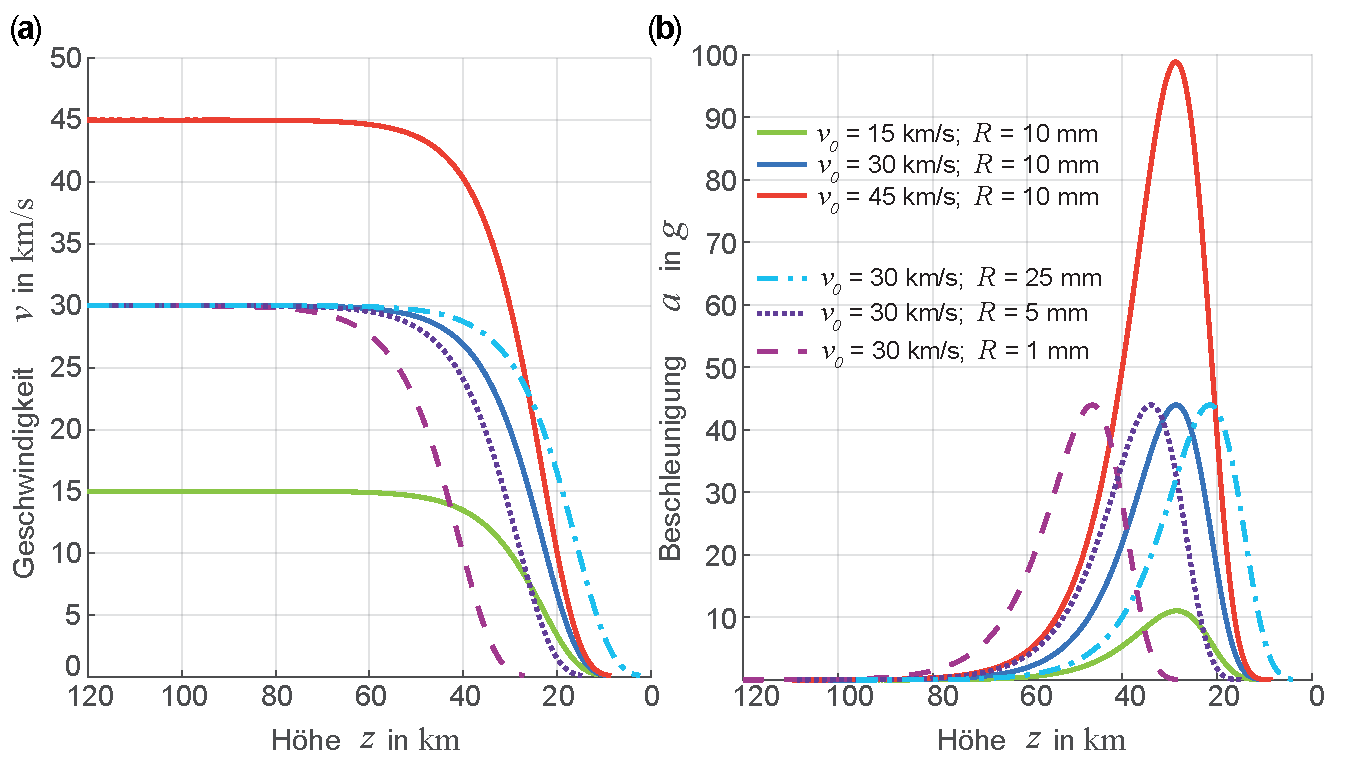
\includegraphics[width=\textwidth]{Meteoroid.pdf}
\caption[Abbremsung eines Meteoroiden in der Erdatmosph�re.]{\fa Geschwindigkeit und \fb Beschleunigung eines Meteoroiden in der Erdatmosph�re. Interessant ist, dass bei �hnlichem Durchmesser die Abbremsung stets in �hnlicher H�he erfolgt. Kleinere/gr��ere Massen/Durchmesser verschieben die H�he zu h�heren/niedrigeren Werten. Bei Anfangsgeschwindigkeiten von $\SI{45}{\km\per\second}$ ergeben sich Bremsverz�gerungen von bis zu $100\,g$.}\label{abb:bew_Meteoroid}
\end{figure}

\subsubsection{Achterbahn} \label{kap:rollercoaster}

Achterbahnen (\figref{bew_Achterbahn01}a), wie generell die Schaustelleranlagen auf den Jahrm�rkten, bieten ein reichhaltiges Angebot f�r physikalische Finger�bungen.\footnote{Achterbahnen sind nicht nur dankbare Studienobjekte f�r die Mechanik. Da Achterbahnz�ge mehrere Tonnen wiegen und Geschwindigkeiten deutlich �ber $\SI{100}{\km\per\hour}$ erreichen, kommen besondere Brems- und Beschleunigungssysteme zum Einsatz. Im der Elektrodynamik werden wir die Physik von Wirbelstrombremsen und linearen Induktionsmotoren behandeln, die beide auf Achterbahnen zum Einsatz kommen.} So ist es nicht verwunderlich, dass es dazu bereits eine Vielzahl von B�chern auf allgemein verst�ndlicher Basis (\zb \cite{Pendrill2021, Weisenberger2013, DPG2012}) gibt.

\begin{figure}
  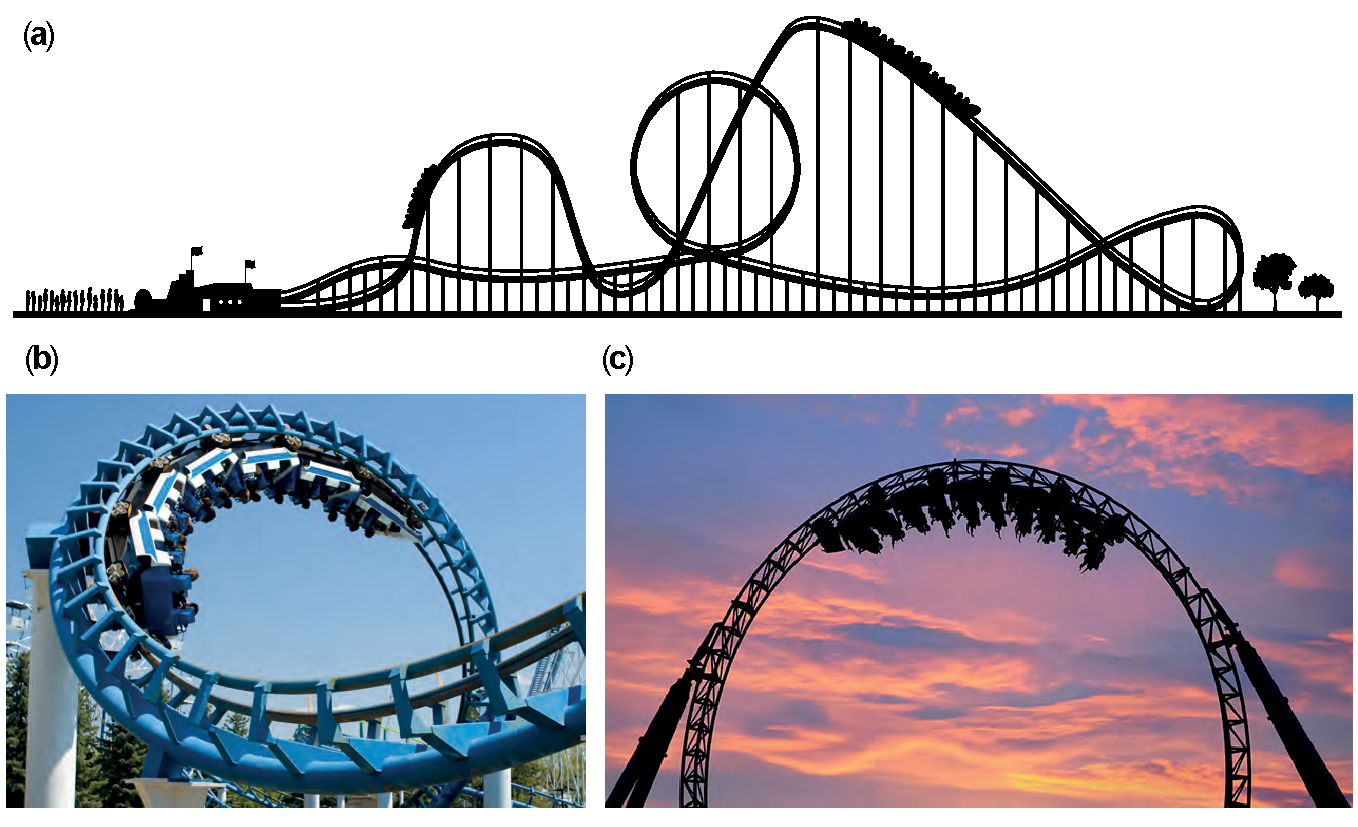
\includegraphics[width=0.95\textwidth]{Achterbahn01.pdf}
  \caption[Typischen Verl�ufe von Achterbahnen mit Looping-Elementen.]{Typischen Verl�ufe von Achterbahnen mit Looping-Elementen. \fa Schema eines typischen Verlaufes. \fb,~\fc Loopings.} \label{abb:bew_Achterbahn01}
\end{figure}

Wer schon mal eine Achterbahn gefahren ist, der hat gesp�rt, wie gro� die Kr�fte sind, die dabei wirken. Sie machen den eigentlichen Nervenkitzel bei den Abfahrten und Loopings erst aus. So kann w�hrend der Fahrt die Beschleunigung des Wagens genauso gro� werden wie die Beschleunigung eines K�rpers im freien Fall. Der Mitfahrer kann dann sein eigenes Gewicht nicht mehr sp�ren und f�hlt sich kurzzeitig in der Luft (auch "`\textit{Airtime}"' genannt) und quasi schwerelos. Die Erkl�rung daf�r kann relativ einfach mit der Newtonschen Mechanik im mitbewegten Koordinatensystem gegeben werden.\\
F�hrt der Wagen durch ein Tal oder eine Kurve, wird die Bewegungsrichtung durch die von den Schienen ausge�bte Zwangskraft auf eine bogenf�rmige Bahn gelenkt. Als Folge dessen sp�rt der Passagier eine Zentrifugalkraft. Im Tal wirken Zentrifugalkraft und Gravitation in dieselbe Richtung. Der Fahrgast f�hlt sich abh�ngig von Kurvenradius \bzw -kr�mmung und Geschwindigkeit deutlich schwerer als sonst. F�hrt der Wagen �ber einen Berg, wirkt die Zentrifugalbeschleunigung vom Wagen weg. Falls diese betragsm��ig gr��er als die Erdbeschleunigung $g$ wird, wird der Mitfahrer nur noch durch einen Gurt im Wagen gehalten.\\
Bei einem Looping (\figref{bew_Achterbahn01}b,c) durchf�hrt der Wagen eine Schleife und befindet sich f�r eine bestimmte Zeit �ber Kopf. Die Zentrifugalkraft im h�chsten Punkt des Loopings muss dann mindestens so gro� sein wie die Gewichtskraft.\\
Mit diesem Wissen k�nnen wir nun sehr einfach berechnen, wie gro� die Geschwindigkeit sein muss, die ein Wagen haben muss, der ein kreisf�rmiges Looping mit Radius $R$ durchf�hrt. Wir werden das f�r einfache F�lle der Achterbahn (Kreisbahn) auf Basis der Newtonschen Mechanik tun. Die Berechnung f�r beliebige Kurvenformen und Zugl�ngen ist mathematisch etwas aufwendiger und wir wollen uns in \probref{bew_achterbahn} etwas grunds�tzlicher mit der Physik auf beliebig gekr�mmten Kurven besch�ftigen und besonders vertieft auch Z�ge in Achterbahnen betrachten. Dabei wollen wir in der �bung auch den Lagrange-Formalismus erster Art \index{Lagrange-Gleichung!Erster Art} benutzen. 

\subparagraph{\textbf{Einzelner Wagen im kreisf�rmigen Looping}}

Wir beginnen die Betrachtung mit einem einzelnen Wagen, der eine kreisf�rmiges Looping fahren soll. Den Wagen betrachten wir als Massepunkt.
Am oberen Punkt des Loopings muss die Zentrifugalkraft gleich der Gewichtskraft sein:
\begin{align*}
    \frac{m\,v_\text{F}{}^2}{R} = m\,g ~~ \rightarrow ~~ v_\text{F}{}^2 = g\,R
\end{align*}
Andererseits muss die Anfangsgeschwindigkeit $v_0$ am Boden gro� genug sein, damit der Massepunkt die H�he $ H = 2R$ erreichen und dann noch eine Geschwindigkeit von $v_\text{F}$ hat, \dh 
\begin{align}
    \frac{m}{2}\,v_0{}^2 &= 2\,m\,g\,R + \frac{m}{2}\,v_\text{F}{}^2 ~~\rightarrow ~~ \frac{v_0{}^2}{2} =  2\,g\,R + \frac{1}{2}\,g\,R ~~\rightarrow~~v_0 = \sqrt{5\,g\,R} \label{eq:bew_Achterbahn01}
\end{align}
Wird der Wagen von einer H�he $H_0$ gestartet, muss diese wegen $2\,g\,H_0 = v_0{}^2$ also mindestens $H_0 = \frac{5}{2}\,R$ betragen. \\

Die Situation ist etwas komplexer, wenn man die Reibung ber�cksichtigt und gleichzeitig eine Einfahrt in das kreisf�rmige Looping nach \figref{bew_loop2loop} betrachtet. Dieses Problem wird in der (angels�chsischen) Literatur als \textit{Loop-the-Loop}-Problem bezeichnet.\index{Loop-the-Loop-Problem}. Am Einfahrtspunkt~T wird der Wagen (Massepunkt) bzw. der im rechten Bild gezeigte rollende Ball eine instantan auftretende Radialbeschleunigung zum Mittelpunkt der Kreisschleife hin erfahren, welche der Mitfahrer als starken \textit{Ruck} (englisch \textit{Jerk})\index{Ruck}\index{Jerk} empfinden w�rde. 

\begin{figure}
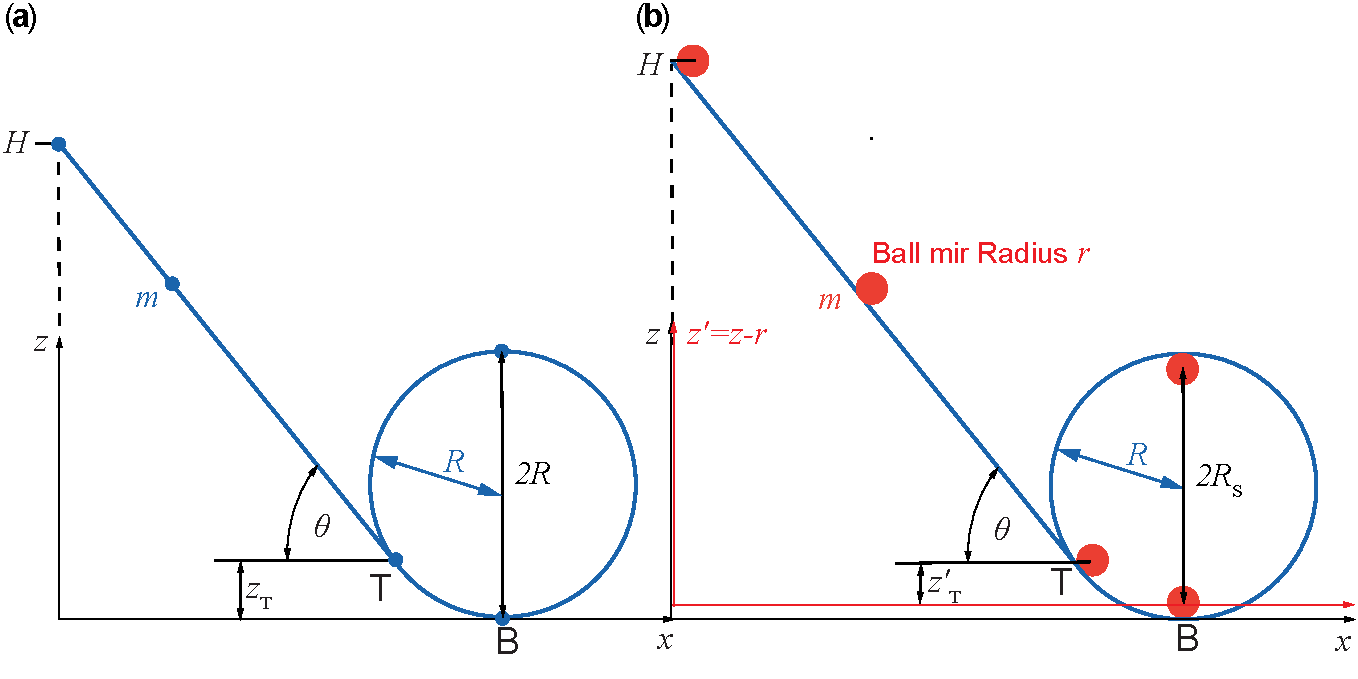
\includegraphics[width=\textwidth]{Loop2Loop.pdf}
\caption[Loop-the-Loop-Problem.]{\fa \textit{Loop-the-Loop}-Problem f�r einen Massepunkt. \fb \textit{Loop-the-Loop}-Problem f�r einen Ball mit Radius $r$.}\label{abb:bew_loop2loop}
\end{figure}

Wir wollen den Massepunkt (als Modell f�r einen einzelnen Wagen) auf der Bahn nach \figref{bew_loop2loop}a untersuchen und auch die Reibung ber�cksichtigen. Dabei wollen wir den auftretenden Ruck genauer untersuchen. Wir m�ssen drei Phasen der Bewegung unterscheiden:
\begin{enumerate}
    \item \textbf{Gleiten auf der geneigten Ebene} von $z=H$ bis zum Punkt T. Diesen Teil k�nnen wir analytisch berechnen und erhalten am Punkt T zum Zeitpunkt $t$ 
    \begin{align*}
        t_\text{T} = \sqrt{\frac{2\,\lk H-z\text{T}\rk}{g\,\lk\sin\theta - \mu_\text{G}\,\cos\theta\rk}}\,,
    \end{align*}
    die Geschwindigkeit
    \begin{align}
        v_\text{T} = \sqrt{2\,\lk H-z\text{T}\rk\,g\,\lk \sin\theta - \mu_\text{G}\,\cos\theta\rk } \label{eq:bew_Achterbahn60} \,,
    \end{align}
    worin $\mu_\text{G}$ der Gleitreibungskoeffizient ist. 
    \item \textbf{Eintritt in das Looping beim Punkt T }\\
    Diesen Abschnitt k�nnen wir nur numerisch berechnen. Am Eintrittspunkt f�hrt die pl�tzlich auftretende, durch die Schienen vermittelte Zwangskraft (Zentripetalkraft der Loop) zu einer in Richtung des Looping-Mittelpunktes auftretenden starken Beschleunigung (Ruck).\footnote{Den Ruck kann man auch als dritte Zeitableitung der Ortskoordinate verstehen, die sonst in der Physik wenig beachtet wird.} \\
    Die numerische Integration f�hren wir bis zum Punkt B, also $z=0$. Dort finden wir dann die Geschwindigkeit $v_\text{B}$.
    \item \textbf{Eigentliches Looping}\\
    Den Teil der Bewegung in der Loop vom Punkt B kann man interessanterweise analytisch geschlossen behandeln. \cite{Klobus2011}\\
    Wir beschreiben die Bewegung in der Koordinate $\varphi$ (siehe \figref{bew_loop2loop}a). \\
    Die Reibungskraft ist gegeben durch 
    \begin{align}
        F_\text{R} = \mu_\text{G}\,F_\text{N} = \mu_\text{G}\,\lk m\,g\,\cos\varphi + \frac{m}{R}\,v^2\lk\varphi\rk\rk\,.\label{eq:bew_Achterbahn61}
    \end{align}
    Dann gilt der Energieerhaltungssatz unter Ber�cksichtigung der durch die Reibungskraft $F_\text{R}$ \anf{geleisteten} Arbeit $W_\text{R}$
    \begin{align}
        \frac{m}{2}\,v_\text{B}{}^2 = \frac{m\,v^2\lk \varphi\rk}{2} + m\,g\,R\,\lk 1-\cos\varphi\rk + \underbrace{\int\limits_0^{s\lk\varphi\rk} F_\text{R}\lk s'\rk\,\D s'}_{W_\text{R}} \,.\label{eq:bew_Achterbahn62}
    \end{align}
    Mit $s\lk\varphi\rk = R\varphi$ f�r ein kreisf�rmiges Looping und damit $\D s = R\,\D\varphi$ k�nnen wir \eqref{eq:bew_Achterbahn62} integrieren:
    \begin{align*}
        \frac{m\,v^2}{2} =\,&\frac{m\,v_\text{B}{}^2}{2} - m\,g\,R + m\,g\,R\,\cos\varphi - \int\limits_0^{\varphi} F_\text{R}\lk\varphi'\rk\,R\,\D\varphi' \,,\\
        v^2 =\,&v_\text{B}{}^2 -2\,g\,R + 2\,g\,R\,\cos\varphi - 2\,\mu_\text{G}\,g\,\int\limits_0^{\varphi}R\,\cos\varphi'\,\D\varphi'- 2\,\mu_\text{G}\,\int\limits_0^{\varphi} v^2\,\D\varphi' \,,\\
    \end{align*}
    Wir f�hren noch zur Abk�rzung $u=v/\sqrt{g\,R}$, $u_\text{B} = v_\text{B}/\sqrt{g\,R}$ ein und erhalten:
    \begin{align}
        u^2 =\,&u_\text{B}{}^2 + 2\,\lk \cos\varphi - \mu_\text{G}\,\sin\varphi -1\rk - 2\,\mu_\text{G}\int\limits_0^\varphi u^2\lk \varphi'\rk\,\D\varphi'\,. \label{eq:bew_Achterbahn63}
    \end{align}
    Das ist eine sogenannte Volterra \gls{integralgleichung}\footnote{Vito Volterra 1860-1940 war ein italienischer Mathematiker, der vor allem auf den Gebieten der mathematischen Biologie und der Integralgleichungen forschte.}\indexp{Volterra, Vito}\index{Integralgleichung, Volterra-}. Die mathematische Behandlung dieser Integralgleichung geht �ber den Umfang dieses Buches hinaus, man findet aber die L�sung in guten Integraltafeln \cite{Gradshteyn1980, Bron2001} \bzw in \cite{Klobus2011}.\footnote{F�r den mathematische interessierten Leser sei erw�hnt, dass die Gl. \eqref{eq:bew_Achterbahn63} eine vereinfachte Form der Volterra Integralgleichung 2.~Art ist: $y\lk t\rk = H\lk t\rk + \int\limits_a^t K\lk t,s\rk\,y\lk s\rk\,\D s$ und daher relativ einfach zu l�sen ist. } Wir geben hier nur die L�sung an:
    \begin{align}
    \begin{split}
        u^2\lk\varphi\rk =\, &\e^{-2\,\mu_\text{G}\,\varphi}\,\lk u_\text{B}{}^2 + \frac{2\alpha}{\beta}\rk - \frac{2}{\beta}\,\lk \alpha\,\cos\varphi + 3\,\mu_\text{G}\,\sin\varphi\rk\\
        &\text{mit}~~~~ \alpha = 1+4\mu_\text{G}{}^2 ~~~~ \text{und} ~~~~ \beta = 2\mu_\text{G}{}^2 -1 \,. 
    \end{split} \label{eq:bew_Achterbahn64}
    \end{align}
    Damit k�nnen wir die Geschwindigkeit zu jedem Winkel $\varphi$ angeben, haben aber keine Zeitabh�ngigkeit $\varphi\lk t\rk$. Diese m�ssen wir uns numerisch wie gewohnt aus der Lagrange-Gleichung beschaffen, die hier einen Reibungsterm enth�lt. Wir empfehlen dem Leser das als relativ einfache �bung selbst durchzuf�hren.
\end{enumerate}
		%\mscr{} \mlbewref{loop2loop.m}
    Aus \eqref{eq:bew_Achterbahn64} lassen sich aber Aussagen gewinnen, welche Geschwindigkeit $v_\text{B}$ das Teilchen (der Wagen) beim Punkt $B$ haben muss, damit es (er) das Looping erfolgreich durchfahren kann. Wir k�nnen folgende 3 Bedingungen formulieren:
    \begin{align*}
        &\text{Bedingung 1:} ~~~~ u\lk\varphi\rk > 0 ~~~~ \text{f�r} ~~~~ \varphi <\frac{\pi}{2} \\
        &\text{Bedingung 2:} ~~~~ F_\text{N}\lk\varphi\rk > 0 ~~~~ \text{f�r} ~~~~ \frac{\pi}{2}\leq \varphi \leq \frac{3}{2}\,\pi \\
        &\text{Bedingung 3:} ~~~~ u\lk\varphi\rk > 0 ~~~~ \text{f�r} ~~~~ \varphi > \frac{3}{2}\,\pi
    \end{align*}
    Wird Bedingung 1 verletzt, bleibt der Wagen im 1. Quadranten des Loopings stecken, analog bei Verletzung von Bedingung 3 im 4. Quadranten. Wird Bedingung 2 verletzt, dann \anf{f�llt} der Wagen von der oberen Kreish�lfte nach unten, und das will ja nun wirklich niemand. \\
    Man kann relativ einfach aus der L�sung \eqref{eq:bew_Achterbahn64} der Integralgleichung ein Stabilit�tsdiagramm berechnen, in dem man auf der $x$-Achse die Anfangsgeschwindigkeit $v_\text{B}$ (\bzw daraus abgeleitet die Anfangsh�he $H$) und auf der $y$-Achse den Gleitreibungskoeffizienten $\mu_\text{G}$ auftr�gt und die Stabilit�tsgrenzen f�r das jeweilige Parameterpaar bestimmt. Dies sei dem Leser in \probref{bew_loop2loop} empfohlen. Ebenso wollen wir das Problem des rollenden Balls von \figref{bew_loop2loop}b, bei dem wir die vom Ball aufgenommene Rotationsenergie ber�cksichtigen m�ssen, in \probref{bew_loop2loop} untersuchen.
		
\subparagraph{\textbf{Bewegung auf Spiralen}}

		Wir wollen noch eine Bemerkung zum Ruck machen. Das gerade beschriebene Problem des Looping Eintritts am Punkt T tritt immer bei Einfahrt und Ausfahrt von Kurven in Geraden auf, so auch \zb in horizontalen Ebene im Stra�enbau. Die Vermeidung \bzw Minimierung des Rucks wurde durch Benutzung von spezifischen, nicht-kreisf�rmigen Kurvenformen gel�st. Besonders ausgezeichnet hat sich dabei die Klothoide\index{Klothoide}, welche auch als Cornu-Spirale\index{Cornu-Spirale}\indexp{Cornu, Marie Alfred}\footnote{Marie Alfred Cornu (1841-1902) war ein franz�sicher Physiker der sich besonders durch hoch genaue Messtechniken zur Messung der Gravitationskonstante $G$ und der Lichtgeschwindigkeit $c$ auszeichnete.} bekannt ist. \\
    Bei dieser Kurve ist der lokale Kr�mmungsradius $\varrho$ invers zur Bogenl�nge $s$:
    \begin{align*}
        \varrho = \frac{p^2}{s}\,,
    \end{align*}
    worin $p$ der sogenannte Klothoidenparameter ist. Die Klothoide kann durch folgende Integraldarstellung \figref{bew_Klothoide} beschrieben werden:
    \begin{subequations}
        \begin{align}
            x\lk t\rk &= p\,\sqrt{\pi}\int\limits_0^t\cos\lk \frac{\pi}{2}\,t'{}^2\rk\,\D t' ~~~~ \text{mit} ~~~~ t = \frac{s}{\sqrt{p\,\pi}}\;,  \label{eq:bew_Achterbahn65a}\\
            z\lk t\rk &= p\,\sqrt{\pi}\int\limits_0^t\sin\lk \frac{\pi}{2}\,t'{}^2\rk\,\D t' ~~~~ \text{mit} ~~~~ t = \frac{s}{\sqrt{p\,\pi}}\;.\label{eq:bew_Achterbahn65b}
        \end{align}
    \end{subequations}

\begin{figure}
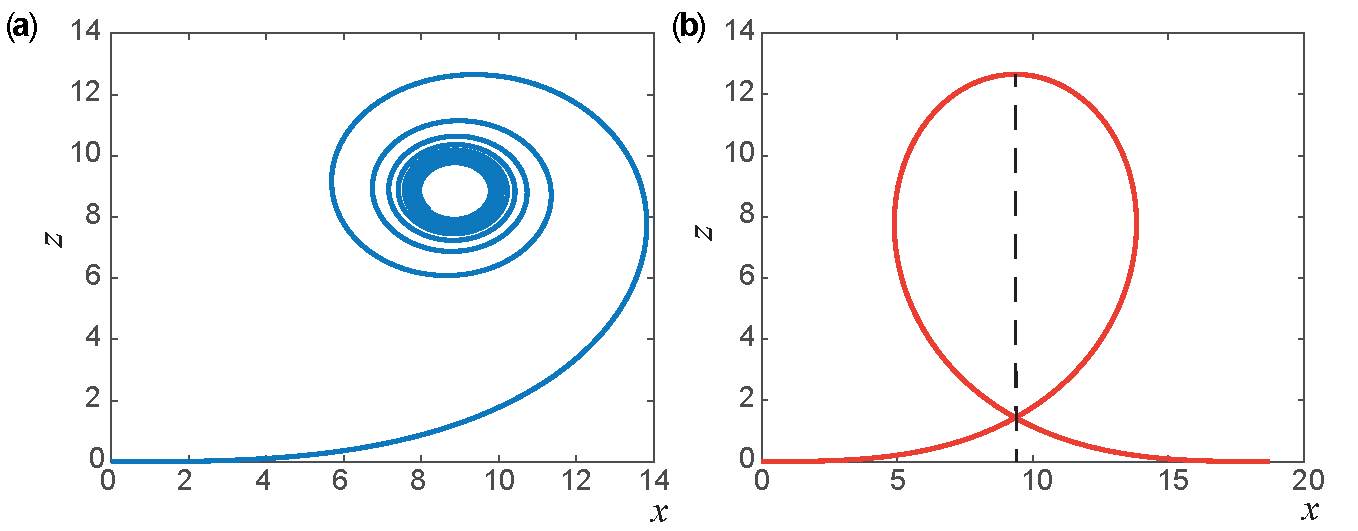
\includegraphics[width=\textwidth]{Klothoide.pdf}
\caption[Klothoide und Looping in Form zweier Klothoiden�ste.]{\fa Klothoide und \fb Looping in Form zweier Klothoiden�ste. Berechnung im  \mscr{} \mlbewref{Klothoide.m}.}\label{abb:bew_Klothoide}
\end{figure}

    F�r ein Stra�en- \bzw Achterbahndesign nimmt man nat�rlich nur den Ast bis zum ersten positiven Maximum und spiegelt dann die Kurve. Bei den Stellen  $s=0 $ und $s=2\,s_\text{max}$ wird dann beim Einfahren aus einer Geraden kein Ruck auftreten, da dort der Kr�mmungsradius $\infty$ ist (siehe auch \cite{Heintz2009}).


\subparagraph{\textbf{Zug im kreisf�rmigen Looping}}

Wir wollen nun den Zug der L�nge $l_\text{Z}$ in einen Kreis-Looping mit dem Radius $R$ untersuchen, was die Situation etwas komplexer macht. Es gibt neben der Zentrifugalkraft eine zus�tzliche Spannungskraft zwischen den einzelnen Wagen des Zuges, die tangential zu der Bahn wirkt und daf�r sorgt, dass alle Wagen im Zug die gleiche Geschwindigkeit und tangentiale Beschleunigung haben. Der Zug habe eine homogene Massenverteilung $\mu = M/l_\text{Z}$. Wir w�hlen das KOS entsprechend \figref{bew_ZugKreisring}. In der Abbildung haben wir zwei Situationen dargestellt, die im Folgenden auch gesondert untersucht werden m�ssen. Sobald der Zug im Loop eingefahren ist, kann das System mit der generalisierten Koordinate $\varphi_\text{F}$ beschrieben werden.\\
Wir wollen berechnen, mit welcher Mindestgeschwindigkeit der Zug in die Kreisbahn-Loop einfahren muss, damit er st�ndig im Kontakt mit der Bahn bleibt. Dazu gen�gt es, die Energieerhaltung und die Spannungskr�fte innerhalb des als Seils/Kette beschriebenen Zuges zu ber�cksichtigen. Ein Massenelement innerhalb des Zuges (in der Loop) ist gegeben durch:
\begin{align}
    \D m = \mu\,R\,\D\varphi = \frac{M}{l_\text{Z}}\,R\,\D\varphi\,. \label{eq:bew_Achterbahn41}
\end{align}
Aus der Energieerhaltung folgt:
\begin{align}
    \frac{M}{2}\,v_0{}^2 = \underbrace{\frac{M}{2}\,v_\text{F}{}^2}_{T\lk \varphi_\text{F}\rk} + \underbrace{\int\limits_{\varphi_\text{E}}^{\varphi_\text{F}} \mu\,g\,R^2\,\lk 1-\cos\varphi\rk\,\D\varphi}_{U\lk \varphi_\text{F}\rk}\,.\label{eq:bew_Achterbahn42}
\end{align}

\begin{figure}
\begin{minipage}{\textwidth}
\leftfigure{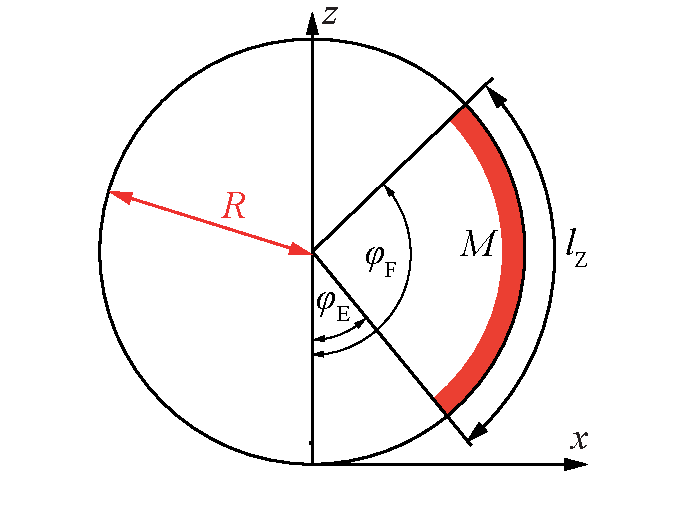
\includegraphics[width=0.5\textwidth]{AchterbahnKreisring.pdf}}%
\hspace{\fill} 
\rightfigure{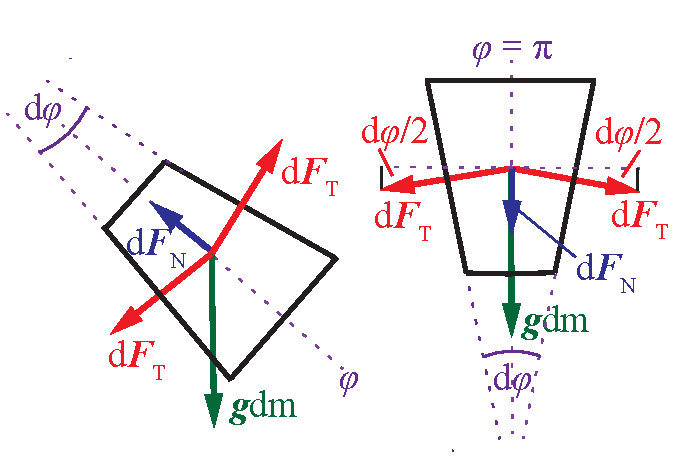
\includegraphics[width=0.5\textwidth]{AchterbahnTangentialK.pdf}}%
\leftcaption[Zug in einem Kreisring als Beispiel f�r ein Looping.]{Zug in einem Kreisring als Beispiel f�r ein Looping.} \label{abb:bew_ZugKreisring}
\rightcaption[Tangentialkr�fte in einem Seil im Kreisring.]{Tangentialkr�fte in einem Seil im Kreisring.} \label{abb:bew_Spannungskraefte}
\end{minipage}
\end{figure}

Hierin sind $v_0$ die Anfangsgeschwindigkeit des Zuges, $v_\text{F}$ die momentane Geschwindigkeit des Zuges wenn der Zuganfang sich bei $\varphi_\text{F}$ befindet ($v_\text{F} = R\,\dot{\varphi}_\text{F}$). Der Potentialterm $U\lk \varphi_\text{F}\rk$ ergibt sich mit der Position des Zugendes $\varphi_\text{E}$ aus der Integration zu:
\begin{subequations}
\begin{align}
  \text{(a): }&~~l_\text{Z}> R\,\varphi_\text{F}\;,~~ \varphi_\text{E}=0 \;, \nonumber \\
		U\lk \varphi_\text{F}\rk &=  \mu\,g\,R^2\,\lek \varphi_\text{F} - \sin\varphi_\text{F}\rek ~~ \,, \label{eq:bew_Achterbahn43a} \\
  %\text{(b):}~~  U\lk \varphi_\text{F}\rk &=  \mu\,g\,R^2\,\lek \frac{l_\text{Z}}{R} - \lk \sin\varphi_\text{F} - \sin\lk \varphi_\text{F} - \frac{l_\text{Z}}{R}\rk \rek ~~ &\text{f�r} ~~ l_\text{Z} < R\,\varphi_\text{F} \equiv \varphi_\text{E} = \varphi_\text{F} - \frac{l_\text{Z}}{R} > 0\,, \varphi_\text{F}\leq 2\pi \, \label{eq:bew_Achterbahn43b}
  % TODO: in der oben auskommentierten Zeile fehlte ein \rk, ich habe unten das \lk entfernt
  \text{(b): }&~~l_\text{Z} < R\,\varphi_\text{F} \,,~~ \varphi_\text{E} = \varphi_\text{F} - \frac{l_\text{Z}}{R} > 0\,,~~ \varphi_\text{F}\leq 2\pi \, \nonumber \\
		U\lk \varphi_\text{F}\rk &=  \mu\,g\,R^2\, \lek \frac{l_\text{Z}}{R} - \sin\varphi_\text{F} + \sin\lk \varphi_\text{F} - \frac{l_\text{Z}}{R}\rk \rek ~\,.\label{eq:bew_Achterbahn43b}
\end{align}
\end{subequations}
Aus \eqref{eq:bew_Achterbahn42} folgt 
\begin{subequations}
\begin{align}
    \text{(a):} ~~ v_\text{F}{}^2 &= v_0{}^2 - \frac{2\,\mu\,g\,R^2}{M}\,\lk \varphi_\text{F} - \sin\varphi_\text{F}\rk\,,\label{eq:bew_Achterbahn44a} \\
    %\text{f�r den Fall (b):} ~~ v_\text{F}{}^2 = v_0{}^2 - \frac{2\,\mu\,g\,R^2}{M}\,\lk \frac{l_\text{Z}}{R} - \lk \sin\varphi_\text{F} - \sin\lk \varphi_\text{F} - \frac{l_\text{Z}}{R}\rk \rk\,,\label{eq:bew_Achterbahn44b}
    % TODO: in der oben auskommentierten Zeile fehlte ein \rk, ich habe unten das \lk entfernt
    \text{(b):} ~~ v_\text{F}{}^2 &= v_0{}^2 - \frac{2\,\mu\,g\,R^2}{M}\,\lk \frac{l_\text{Z}}{R} - \sin\varphi_\text{F} + \sin\lk \varphi_\text{F} - \frac{l_\text{Z}}{R}\rk \rk\,,\label{eq:bew_Achterbahn44b}
\end{align}
\end{subequations}
woraus man sehr einfach die Differentialgleichung f�r den Zug ableiten kann, in dem man \eqref{eq:bew_Achterbahn44a} \bzw \eqref{eq:bew_Achterbahn44b} nach der Zeit differenziert, woraus man wiederum die zeitliche Entwicklung f�r $\varphi$ numerisch in \matlab{} berechnen kann. \\

\begin{nebenrechnung}

\begin{subequations}
\begin{align}
    \text{(a):}&~~ v_\text{F}{}^2 = R^2\,\dot{\varphi}_\text{F}{}^2 = v_0{}^2 - \frac{2\,\mu\,g\,R^2}{M}\,\lk \varphi_\text{F} - \sin\varphi_\text{F}\rk \nonumber \\
    %2\,R^2\,\dot{\varphi}_\text{F}\,\ddot{\varphi}_\text{F} &= -\frac{2\,\mu\,g\,R^2}{M}\,\lk\dot{\varphi}_\text{F} - \cos\varphi_\text{F}\,\dot{\varphi}_\text{F}\rk \nonumber \\
    \rightarrow ~~~~ \ddot{\varphi}_\text{F} &=  \frac{\mu\,g}{M}\,\lk \cos\varphi_\text{F} - 1\rk  \label{eq:bew_Achterbahn45a} \\
		\nonumber \\
    \text{(b):} &~~ v_\text{F}{}^2 = R^2\,\dot{\varphi}_\text{F}{}^2 = v_0{}^2 - \frac{2\,\mu\,g\,R^2}{M}\,\lek \frac{l_\text{Z}}{R} -\,\lk \sin\varphi_\text{F} - \sin\lk \varphi_\text{F} - \frac{l_\text{Z}}{R}\rk\rk\rek \nonumber \\
    \rightarrow ~~~~ \ddot{\varphi}_\text{F} &= \frac{\mu\,g}{M}\,\lek \cos\varphi_\text{F} - \cos\lk \varphi_\text{F}-\frac{l_\text{Z}}{R}\rk\rek \label{eq:bew_Achterbahn45b}
\end{align}
\end{subequations}

\end{nebenrechnung}

Wir ben�tigen jetzt noch wie eingangs erw�hnt die internen Spannungskr�fte im Zug (Seil), also die Kr�fte die zwischen den einzelnen Wagen von den Kupplungen vermittelt werden. Wir k�nnten uns diese aus den Lagrange-Multiplikatoren beschaffen (siehe \probref{bew_achterbahn}). Es gibt aber einen etwas einfacheren Weg, in dem wir die an jedem Massenelement am Ort $\varphi$ wirkenden differentiellen Tangentialkr�fte integrieren. Die differentielle Tangentialkraft ist nach \figref{bew_Spannungskraefte} gegeben durch:
\begin{align}
     \D F_\text{T} &= \D m\,g\,\sin\varphi = g\,\mu\,R\,\sin\varphi\,\D \varphi \nonumber \\
     \rightarrow ~~~~ F_\text{T}\lk \varphi\rk &= \int\limits_{\varphi_\text{E}}^{\varphi}g\,\mu\,R\,\sin\varphi\,\D\varphi = -g\,\mu\,R\,\cos\varphi\,\Big|_{\varphi_\text{E}}^{\varphi} ~~~(\varphi_\text{E} \geq 0) \,.\label{eq:bew_Achterbahn47}
\end{align}
$F_\text{T}\lk \varphi\rk$ ist die am \anf{Ort} $\varphi$ wirkende Tagentialkraft, die wir in der differentiellen N�herung als interne Spannungskraft verstehen k�nnen. Die kritische Situation f�r den Zug in der Loop besteht wenn der Mittelteil des Zuges am oberen Punkt der Loop angekommen ist, \dh
\begin{align*}
    \varphi_\text{F} &= \pi + \frac{l_\text{Z}}{2R}\,, & \varphi_\text{E} = \pi - \frac{l_\text{Z}}{2R}\,, ~~~~ l_\text{Z} \leq 2\pi R  \,.
\end{align*}
F�r den Betrag der Tangentialkraft gilt:
\begin{align}
    F_\text{T}\lk\varphi=\pi\rk & = -g\,\mu\,R\,\cos\varphi\,\Big|_{\pi-\frac{l_\text{Z}}{2R}}^\pi = -g\,\mu\,R\,\lek -1-\cos\lk\pi-\frac{l_\text{Z}}{2R}\rk\rek \nonumber \\
		& = g\,\mu\,R\,\lek 1-\cos\lk\frac{l_\text{Z}}{2R}\rk\rek \; . \label{eq:bew_Achterbahn48}
\end{align}
Am oberen Punkt des Kreises muss die differentielle Kr�ftebilanz wie folgt aussehen:
\begin{align}
    \D \vec{F}_\text{G} + \D \vec{F}_\text{N}\lk \pi \rk  = \D \vec{F}_\text{G} + \D \vec{F}_\text{T}\lk \pi \rk   = \D \vec{F}_\text{Z}\,, \label{eq:bew_Achterbahn48a}
\end{align}
worin $\D \vec{F}_\text{Z}$ die auf das Massenelement $\D m$ wirkende Zentrifugalkraft mit $R\dot{\varphi}_\text{F}^2\,\D m = R\dot{\varphi}\,\lk \pi + \frac{l_\text{Z}}{2R}\rk^2 \,\D m$ ist. Wir benutzen \figref{bew_Spannungskraefte} und setzen \eqref{eq:bew_Achterbahn48} sowie \eqref{eq:bew_Achterbahn44a} in \eqref{eq:bew_Achterbahn48a} ein und erhalten f�r die $z$-Komponente der Kr�ftebilanz \eqref{eq:bew_Achterbahn48a}:
\begin{align}
    g\,\D m + 2\,g\,\mu\,R\,\lk 1 - \cos\lk \frac{l_\text{Z}}{2R}\rk\rk\,\sin\lk \frac{\D \varphi}{2}\rk &= R\,\dot{\varphi}_\text{F}{}^2\,\D m \nonumber \\
    \mu\,g\,R\,\D\varphi + 2\,g\,\mu\,R\,\lk 1-\cos\lk \frac{l_\text{Z}}{2R}\rk\rk\, \frac{\D \varphi}{2} &\approx \mu\,R^2\,\dot{\varphi}_\text{F}{}^2\,\D\varphi \nonumber \\
    \rightarrow~~~ \frac{g}{R}\,\lk 2-\cos\lk \frac{l_\text{Z}}{2R}\rk\rk & = \dot{\varphi}_\text{F}{}^2 \,. \label{eq:bew_Achterbahn49}
\end{align}
Mit der Beziehung \eqref{eq:bew_Achterbahn44b}, die aus der Energieerhaltung abgeleitet wurde, erhalten wir mit $v_\text{F} = R \dot{\varphi}_\text{F}$,  $\varphi_\text{F} = \pi + l_\text{Z}/2R \, \varphi_\text{E} = \pi - l_\text{Z}/2R $:
\begin{align}
    %v_0{}^2 & = g\,R\,\lk 2-\cos\lk\frac{l_\text{Z}}{2R}\rk\rk + \frac{2\,\mu\,g\,R^2}{M}\,\lek \varphi_\text{F} - \sin\varphi_\text{F} - \lk \varphi_\text{E} - \sin\varphi_\text{E} \rk \rek  \nonumber \\
    v_0{}^2 & =  g\,R\,\lk 2-\cos\lk\frac{l_\text{Z}}{2R}\rk\rk + \frac{2\,\mu\,g\,R^2}{M}\,\lek \frac{l_\text{Z}}{R} + 2\,\sin\lk \frac{l_\text{Z}}{2R}\rk\rek \,. \label{eq:bew_Achterbahn50}
\end{align}
Man kann die Spezialf�lle $l_\text{Z}=0$ (einzelner Wagen als Massepunkt), $l_\text{Z}=2\,\pi\,R$ (Kreisring vollst�ndig gef�llt durch Zug) und $l_\text{Z}=\pi\,R$ (Kreisring zur H�lfte gef�llt durch Zug) leicht berechnen.
\begin{align*}
l_\text{Z} \to 0 ~~ &\text{mit} ~~ \mu{}\,l_\text{Z}/M \to 1: \\
    v_0{}^2(l_\text{Z} \to 0) &= g\,R\, + \lim_{l_\text{Z} \to 0,\mu{}l_\text{Z}/M \to 1}  \lek \frac{\mu}{M} 2 \,g\,R^2 \lk \frac{l_\text{Z}}{R} +2\,\sin\frac{l_\text{Z}}{2R} \rk \rek \\
										 &= \,g\,R \,+ 2 \,g\,R\,(1+1) = 5 \,g\,R \,, \\ \\
l_\text{Z} = 2\pi\,R~~ &\text{mit} ~~ \mu{}\,l_\text{Z}/M = 1: \\
    v_0{}^2(l_\text{Z}=2\pi R) &= g\,R\,\lk 2+1\rk + 2\,\frac{\mu}{M}\,g\,R^2 \lek 2\pi + 2\sin\lk \frac{2\,\pi\,R}{2R}\rk \rek \\
		                 &= 3\,g\,R \,+ 2\,\frac{\mu}{M}\,g\,R^2(2\pi + 0) = 5\,g\,R \,, \\ \\
l_\text{Z} = \pi\,R~~ &\text{mit} ~~ \mu{}\,l_\text{Z}/M = 1: \\ 
    v_0{}^2(l_\text{Z}=\pi R) &= g\,R\,\lk 2 + 0\rk +2\,\frac{\mu}{M}\,g\,R^2 \lek \pi + 2\sin\lk \frac{\pi\,R}{2R}\rk \rek \\
		                 &= 2\,g\,R \,+ 2\,\frac{\mu}{M}\,g\,R^2(\pi + 2) = 2\,g\,R \,\lk 1 + 1 + \frac{2}{\pi} \rk = 4\,g\,R \,\lk 1+ \frac{1}{\pi} \rk \,.
\end{align*}
Das Ergebnis ist insofern interessant, als dass ein Seil der L�nge $2 \pi R$ und gleicher Masse $M$ die gleiche Anfangsgeschwindigkeit braucht wie ein einzelne Massepunkt der Masse $M$ , um die Loop sicher zu durchlaufen (Reibung vernachl�ssigt). Man kann sich das aber auch klar machen, in dem man eine Energiebetrachtung aus dem Inertialsystem heraus macht und ber�cksichtigt, dass dort die Rotationsenergie von Massepunkt und Ring (= Seil) unter den angenommenen Bedingungen gleich gro� sind. 

In \probref{bew_achterbahn} behandeln wir die Dynamik von Massepunkten und Z�gen auf gekr�mmten Kurven (wie sie bei der Achterbahn auftreten) etwas allgemeiner.
%wobei wir ebenfalls das Modell der Kette unter dem Einfluss verschiedener Kr�fte und Zwangsbedingungen betrachten wollen. 
In \probref{bew_achterbahn_diskret} untersuchen wir ein diskretes Modell eines Zuges auf einer beliebigen Kurve, welches wir nach der das in \probref{bew_achterbahn_vergleich} mit dem hier ausgearbeiteten Modell eines starren Zuges der L�nge $l_\text{Z}$ vergleichen.
Mit den in der Mechanik der Kontinua (Kapitel 2) entwickelten Methoden werden wir dann in \probref{kontmech_AchterbahnKont} bis \probref{kontmech_AchterbahnBeschleunigungen} ein Modell eines erweitertes Modell eines "`teilelastischen"' Zuges behandeln k�nnen.

\subsubsection{Dynamik einer fallenden Kette und Bungee-Jumping} \label{kap:bew_chains}

\subparagraph{\textbf{Fallende Kette}} \index{Kette!fallende} 

Ein interessantes Problem ist das der fallenden Kette (siehe auch \cite{Wong2006,Calkin1989}).
Dieses Problem beinhaltet die Dynamik einer ver�nderlichen Masse, wie wir dies in �hnlicher Form beim Raketenstart im Kapitel Astrodynamik betrachten werden.
Interessanterweise wurde das Problem in vielen Lehrb�chern der Physik bis in die 1980er Jahre hinein \zt falsch beschrieben, obwohl bereits Lagrange%
\indexp{Lagrange, Joseph-Louis} alle Methoden zu dessen Behandlung aufgezeigt hatte. 
\begin{figure}
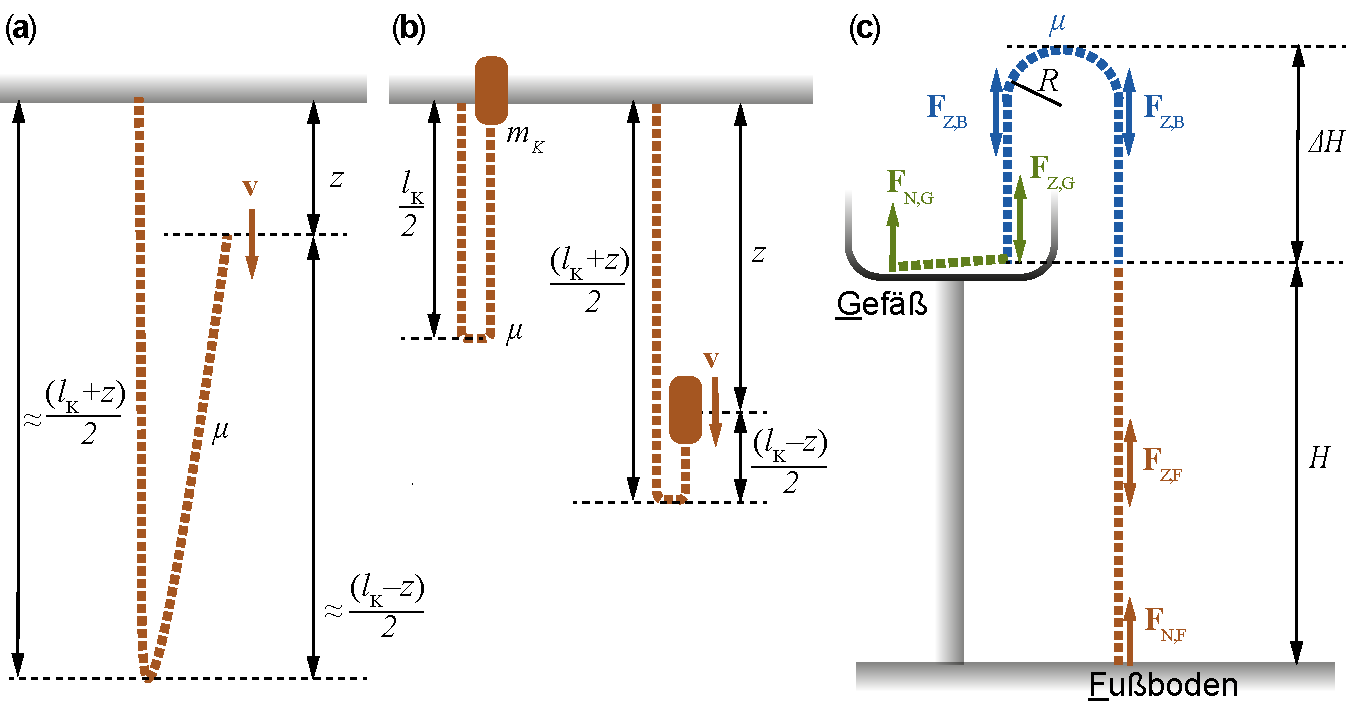
\includegraphics[width=0.95\textwidth]{FallingChain01.pdf}
\caption[Modell der fallenden Kette und Beispiele.]{Modell der fallenden Kette und Beispiele. \fa Grundmodell ($\mu$ Masse der Kette pro L�ngeneinheit. \fb Modell f�r Bungee-Jumping ($m_\text{K}$ Masse des K�rpers, $v$ Geschwindigkeit in Fallh�he $z$. \fc Kettenfont�ne und wirkende Kr�fte. Zur besseren Unterscheidung der Einheiten der Kette sind diese farblich unterschiedlich gekennzeichnet, es handelt sich aber um eine homogene Kette mit der Massendichte $\mu$.}\label{abb:bew_FallingChain01}
\end{figure}
Einer der interessantesten Effekte der fallenden Kette ist die Tatsache, dass das lose Ende der Kette schneller fallen kann als ein K�rper im freien Fall, obwohl als �u�ere Kraft nur die Schwerkraft wirkt. Wir wollen das erkl�ren und schreiben dazu mit \figref{bew_FallingChain01} die Lagrange-Funktion auf:
        \begin{align}
            \mathcal{L}\lk z,\dot{z}\rk = T(z) - U(z) = \frac{\mu}{4}\,\lk l_\text{K}-z\rk\,\dot{z}^2 + M\,g\,\lk \frac{l_\text{K}^2+2z\,l_\text{K}-z^2}{4 l_\text{K}}\rk\,. \label{eq:bew_FallingChain01}
        \end{align}
Wir halten ferner fest, das folgende Beziehungen gelten:
        \begin{align*}
            m_\text{L} &= \mu\,b_\text{L}\,, & m_\text{R}&= \mu\,b_\text{R}\,, \\
            b_\text{L} &= \frac{1}{2}\,\lk l_\text{K}+z\rk\,, & b_\text{R} &= \frac{1}{2}\,\lk l_\text{K}-z\rk \,,\\
            z_\text{L} &= \frac{1}{4}\,\lk l_\text{K}+z\rk\,, & z_\text{R} &= \frac{1}{4}\,\lk l_\text{K}+3z\rk\,,
        \end{align*}
worin $\mu$ die homogene Massendichte $\mu = M/l_\text{K}$, $b_\text{i}$ die L�nge, $z_\text{i}$ der Schwerpunkt, und $m_\text{i}$ die Masse des linken ($i=L$) bzw. rechten ($i=R$) Arms der Kette sind. Offensichtlich ist $\d \mathcal{L}/\d t = 0 $. Die Hamilton-Funktion (siehe Definition \eqref{eq:bew_Hamilton_Fkt})
        \begin{align}
            \mathcal{H} = \underbrace{\frac{\d\mathcal{L}}{\d \dot{z}}\cdot\dot{z}}_{p_\text{R}\,v} - \mathcal{L}\lk z,\dot{z}\rk = \frac{{p_\text{R}}^2}{2m_\text{R}} - M\,g\,\lk \frac{l_\text{K}^2+2z\,l_\text{K}-z^2}{4 l_\text{K}}\rk = E \label{eq:bew_FallingChain03}
        \end{align}
ist daher nach \kapitel{bew_Lagrange_II} gleich der Energie $E$, da das System konservativ ist. Mit der aus der Lagrange-Funktion berechneten Lagrange-Gleichung und unter Verwendung von $\dot{z} = v$ und $\ddot{z} = \dot{v}$ schreiben wir:
%\footnote{Man kann auch einfacher dies aus der Hamilton-Funktion erhalten, indem man $\frac{\d p}{\d t} = -\frac{\d \mathcal{H} t}{\d t}$ bildet.}
        \begin{align}
            \dot{p}_\text{R} = m_\text{R}\,\dot{v} + \dot{m}_\text{R}\,v = m_\text{R}\,g - \frac{1}{4}\,\mu\,v^2 \,.\label{eq:bew_FallingChain04}
        \end{align}
Man erkennt an \eqref{eq:bew_FallingChain04} sehr sch�n die zeitlich ver�nderliche Masse und einen daraus folgenden Zusatzterm $-\frac{1}{4}\,\mu\,v^2$, der der Schwerkraft entgegen wirkt und eine innere Spannung der Kette darstellt. Dieser Term ist f�r die zus�tzliche Beschleunigung des rechten Arms der Kette verantwortlich, der zu gr��eren Fallgeschwindigkeiten f�hrt, als sie im freien Fall auftreten. Gl. \eqref{eq:bew_FallingChain04} ist eine nichtlineare Differentialgleichung.\\
Aus der Energieerhaltung $U_0 = -M\,g\,l_\text{K}/4 = T(z) + U(z)$ findet man leicht
        \begin{align}
        \begin{split}
            v^2\lk z\rk &= 2g\,x\,\frac{\lk 1-\frac{1}{2}\,\frac{z}{l_\text{K}}\rk}{\lk 1-\frac{z}{l_\text{K}}\rk} \\
            &\approx 2g\,z\,\lek 1+\frac{1}{2}\,\lk \frac{z}{l_\text{K}} + \lk \frac{z}{l_\text{K}}\rk^2 +\ldots \rk\rek = {v_\text{F}}^2\,\lek 1+\frac{1}{2}\,\lk \frac{z}{l_\text{K}} + \lk \frac{z}{l_\text{K}}\rk^2 +\ldots \rk\rek\,, \label{eq:bew_FallingChain05}
        \end{split}
        \end{align}
worin $v_\text{F} = \sqrt{2g\,z}$ die Geschwindigkeit des freien Falls ist. \\
Die DGL \eqref{eq:bew_FallingChain04} k�nnen wir numerisch l�sen. %Der Ansatz
	%\[\dot{v} = \frac{1}{2}\,\frac{\D v^2}{\D z} = v\,\frac{\D v}{\D t}\,\frac{\D t}{\D z}
	%\]
%auf eine inhomogene Differentialgleichung f�r $v^2$. 
In \figref{bew_FallingChain02} zeigen wir die numerische L�sung $v\lk t\rk$, $z\lk t\rk$ im Vergleich zum freien Fall (\mlbewref{FallingChain01.m})  Deutlich ist die Beschleunigung gr��er als $g$ zu erkennen.

\begin{figure}
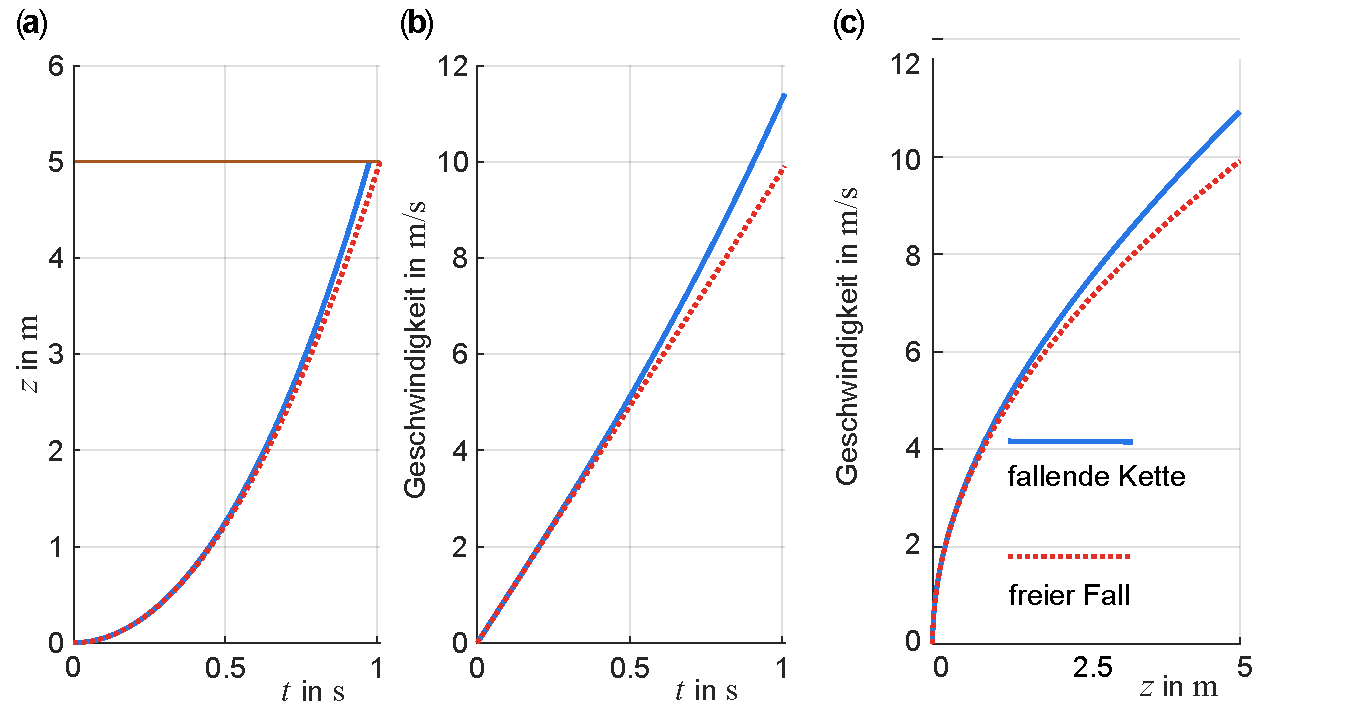
\includegraphics[width=\textwidth]{FallingChain02.pdf}
\caption[Dynamik der fallenden Kette im Vergleich zum freien Fall.]{Dynamik der fallenden Kette im Vergleich zum freien Fall. Man sieht, dass am Ende der Fallperiode die Geschwindigkeit der fallenden Kette gr��er ist als die des freien Falls. Die Fallzeit der Kette in unserem Modell ist unabh�ngig von der Massendichte $\mu$. }\label{abb:bew_FallingChain02}
\end{figure}

Wir wollen jetzt noch eine Erkl�rung daf�r geben, dass die Spannung $F_\text{T} = -\mu\,v^2/4$ in \eqref{eq:bew_FallingChain04} der Schwerkraft entgegen wirkt und nicht, wie man vielleicht erwarten k�nnte, in Richtung von $g$. Schreibt man \eqref{eq:bew_FallingChain04} in Newtonscher Form, also 
        \begin{align*}
            m_\text{R}\,\dot{v} = m_\text{R}\,g - \underbrace{\lk \dot{m}_\text{R}\,v + \frac{1}{4}\,\mu\,v^2 \rk}_{= F_\text{T,eff}}\,,
        \end{align*}
dann ergibt der gesamte Zusatzterm $F_\text{T,eff}$ wegen $\dot{m}_\text{R}<0$ eine zus�tzliche Kraft in Richtung der Schwerkraft. Wir wollen uns jetzt noch zwei konkrete Anwendungen dieser bisher eher theoretischen �berlegungen anschauen. 

\subparagraph {\textbf{Bungee-Jumping}} \index{Bungee-Jumping}

Eine Art "`Kettenproblem"' liegt auch beim Bungee-Jumping (\figref{bew_FallingChain01}b) vor. Die Lagrange-Funktion k�nnen wir wieder einfach aufschreiben, der einzige Unterschied zu \eqref{eq:bew_FallingChain01} ist das Auftreten der Zusatzmasse $m_\text{K}$ des Bungee-Springers.

Die Lagrange Funktion lautet dann:
\begin{align}
\begin{split}
    \mathcal{L} = &T-U \\
    = &\underbrace{\lek \frac{1}{2}\,m\,\frac{l_\text{K}-z}{2 l_\text{K}}\,\dot{z}^2 + \frac{1}{2}\,m_\text{K}\,\dot{z}^2 \rek }_{T} \\
		  &- \underbrace{\lek -m\,\frac{l_\text{K}-z}{2 l_\text{K}}\,g\,\lk z + \frac{l_\text{K}-z}{4}\rk \rek }_{U_1} 
			 - \underbrace{\lek - m\,\frac{l_\text{K}+z}{2 l_\text{K}}\,g\,\frac{l_\text{K}+z}{4} \rek}_{U_2} - \underbrace{m_\text{K}\,g\,z}_{U_3}\,.
\end{split} \label{eq:bew_Bungee01}
\end{align}
Hierin sind $U_1$ die potentielle Energien des bereits gefallenen Bandes, $U_2$ die des noch h�ngenden Bandes und $U_3$ die potentielle Energie des Springers. Die Geschwindigkeit des Springers ergibt sich direkt aus der Energieerhaltung, dabei ist die Anfangsenergie (das Nullpotential liege bei $z=0$) gegeben durch:
\begin{align*}
    E_0 = -m\,g\,\frac{l_\text{K}}{4}\,.
\end{align*}
Daraus folgt mit $E_0 = T + U_1 +U_2+U_3 $ aus \eqref{eq:bew_Bungee01}: 
\begin{align}
    v^2\lk z\rk = \dot{z}^2 = g\,z\,\frac{4m_\text{K}\,l_\text{K} + 2m\,l_\text{K} -m\,z}{m\,l_\text{K}-m\,z + 2m_\text{K}\,l_\text{K}} \label{eq:bew_Bungee02}
\end{align}
und speziell f�r $z=l_\text{K}$ (am Ende des Sprunges) zu
\begin{align}
    v_\text{f}{}^2 = v^2\lk l_\text{K}\rk = 2g\,l_\text{K} + \frac{1}{2}\,\frac{m}{m_\text{K}}\,g\,l_\text{K} \,. \label{eq:bew_Bungee03}
\end{align}
Man erkennt, dass f�r $m_\text{K} \gg m$ dies in die Beziehung f�r den freien Fall �bergeht.  \\
Durch Differenzieren nach $t$ finden wir die Beschleunigung $a\lk z\rk =\D v/\D t$:
\begin{align}
    a\lk z\rk = g\,\lek 1 + \frac{m\,z\,\lk 4m_\text{K}\,l_\text{K}+2m\,l_\text{K}-m\,z \rk}{2\lk m\,l_\text{K} -m\,z + 2m_\text{K}\,l_\text{K}\rk^2}\rek\,. \label{eq:bew_Bungee04}
\end{align}
Wiederum gilt:
\begin{align*}
    \lim_{m\to 0}a\lk z\rk = g\,\lek 1+0\rek = g\,.
\end{align*}
F�r $m\neq 0$ folgt $a\lk z\rk > g$ f�r alle $z$ und der Maximalwert ergibt sich bei $z= l_\text{K}$ zu :
\begin{align*}
    a\lk l_\text{K}\rk &= g\,\lek 1+\frac{m\lk 4m_\text{K} + m\rk}{8m_\text{K}{}^2}\rek = g\,\lek 1+\frac{q\,\lk 4+q\rk}{8}\rek \,,
\end{align*} 
worin $q= m/m_\text{K}$ das Verh�ltnis der Massen von Band und Springer ist. 

\begin{figure}
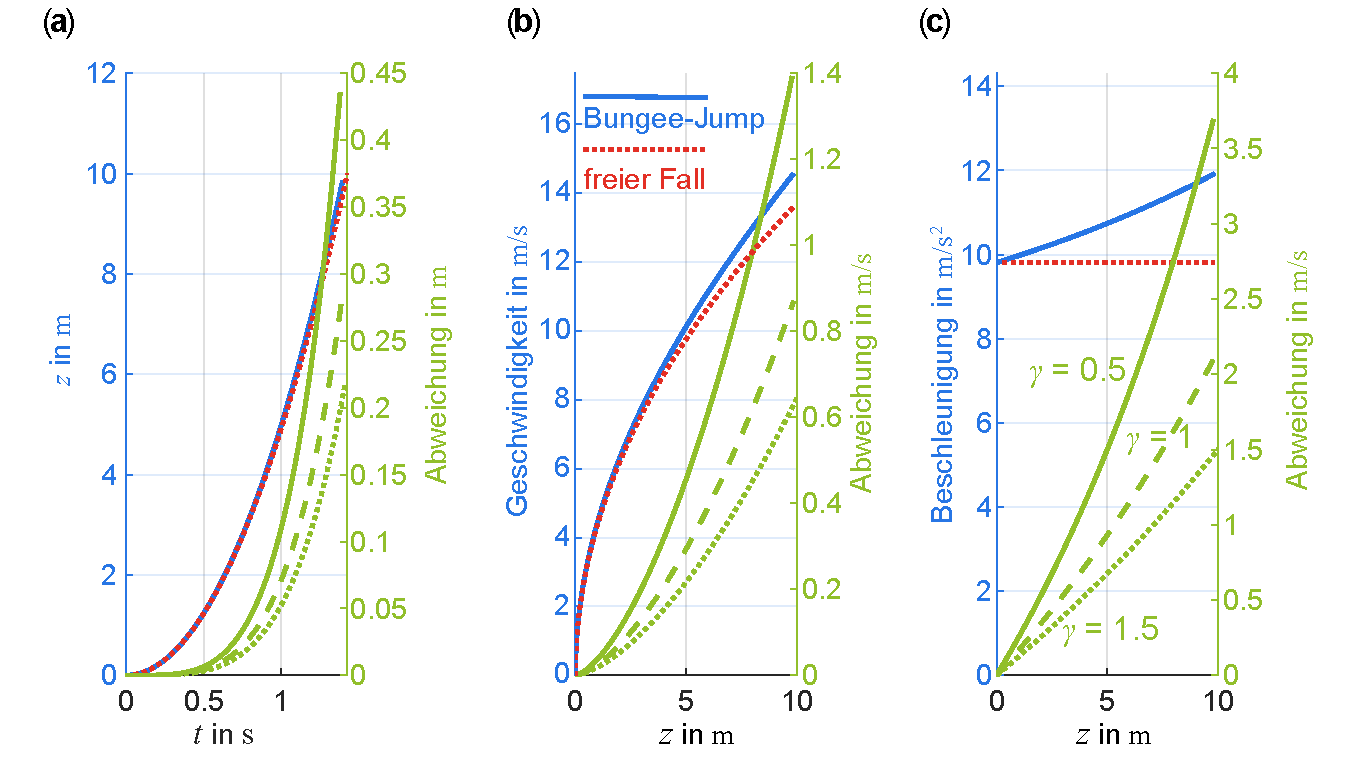
\includegraphics[width=\textwidth]{FallingChain03.pdf}
\caption[Dynamik des Bungee Jumping.]{%
Dynamik des Bungee Jumping. Parameter: Volle Seill�nge  $l_\text{K}=\SI{20}{\metre}$.
\fa Durchlaufene Fallstrecke als Funktion der Zeit.
Der \anf{Zuwachs} an Fallstrecke gegen�ber dem freien fall ist relativ gering und umso gr��er, je schwerer das Seil im Vergleich zum fallenden K�rper ist.
\fb Die analoge Darstellung f�r die Fallgeschwindigkeit.
Auch hier der Unterschied zum freien Fall sichtbar gr��er, je schwerer das Seil im Vergleich zum fallenden K�rper ist.
\fc Beschleunigung als Funktion der durchlaufenen Fallstrecke.
Man erkennt in der Abweichung $a\lk z\rk -g $ sehr sch�n, dass am Ende der Fallstrecke eine deutliche gr��ere Beschleunigung als $g$ auf den K�rper wirkt.}
\label{abb:bew_Bungee01}
\end{figure}

In \figref{bew_Bungee01} ist die Funktion $z\lk t\rk$ f�r den Bungee-Jumper f�r verschiedene Parameters�tze $q = m_\text{K}/m$
im Vergleich zum freien Fall dargestellt (\mscr{} \mlbewref{BungeeJumping.m}).
Man erkennt, dass in der Tat erhebliche gr��ere Beschleunigungen als $g$ auftreten k�nnen.
Wir wollen allerdings darauf hinweisen, dass wir in unserem Modell Energieerhaltung angenommen haben ($U_0 = T_\text{final}$),
was bei realen B�ndern nicht unbedingt gegeben sein muss. Au�erdem haben wir nicht ber�cksichtigt, dass bei Erreichen von $z=l_\text{K}$ das Band/Seil hinreichend elastisch sein sollte, damit der Springer vor Verletzungen gesch�tzt ist.

\subparagraph {\textbf{Enterhaken, Harpune}} 

Mit dem Problem des Bungee-Jumping eng verwandte Probleme sind das Werfen eines Enterhakens \cite{Mungan2022}, das Abschie�en einer Harpune oder das Werfen eines Lassos/Anlegetaus. Im Prinzip ist dies die Umkehrung des Bungee-Jumpings bzw. der fallenden Kette, wobei die geworfene Kette hier wieder die zus�tzliche Masse $m_\text{K}$ am Ende tragen kann (\figref{bew_FallingChain01}b). Wir k�nnen die Lagrange-Funktion schreiben als: 
        \begin{align}
            \mathcal{L} = \frac{M}{2}\,\dot{z}^2 - \frac{z^2}{2}\,g\,\mu\,. \label{eq:bew_Harpune01}
        \end{align}
Hierin haben wir einfacherweise  die Abschussrichtung $z$ senkrecht nach oben gew�hlt, $\mu$ ist wieder die Massendichte des Seils in $\SI{}{\g\per\cm}$, $M = m_\text{K}+\mu\,z$ die Gesamtmasse mit $m_\text{K}$ der Hakenmasse. Aus \eqref{eq:bew_Harpune01} folgt die Lagrange-Gleichung
        \begin{align}
            \lk m_\text{K} +\mu\,z\rk\,\ddot{z} + \mu\,\dot{z}^2 + \lk m_\text{K} + \mu\,z\rk\,g = 0\,, \label{eq:bew_Harpune02}
        \end{align}
was auch mit $P = M\,v$ einfach geschrieben werden kann als 
        \begin{align}
            \frac{\D P}{\D t} = \frac{\D}{\D t}\,\lk M\,v\rk = -M\,g ~~~~ \text{mit} ~~~~ v=\dot{z}\,. \label{eq:bew_Harpune03}
        \end{align}
Diese Gleichung kann nach der Geschwindigkeit $v$ als Funktion der H�he $z$ gel�st werden.
        \begin{align}
            \frac{\D P}{\D t} &= \frac{\D P}{\D z}\,\frac{\D z}{\D t}  = \frac{\D P}{\D z} \,\frac{P}{M}\,= -M\,g  \, \nonumber \\
            \rightarrow ~~~~ -P\,\D P &= g\,M^2\,\D z = g\,\lk m_\text{K} + \mu\,z\rk^2\,\D z \,.  \label{eq:bew_Harpune04a}
			  \end{align}
Integration von \eqref{eq:bew_Harpune04a} ergibt 
        \begin{align}
            m_\text{K}\,{v_0}^2 - M\,v^2 &= \frac{2g}{3\mu}\,\lk M^3-m_\text{K}\rk \nonumber \\
            \rightarrow ~~~~ v &= \lk 1+ \frac{\mu\,z}{m_\text{K}}\rk^{-1}\,\sqrt{{v_0}^2 - \frac{2m_\text{K}\,g}{3\mu}\,\lek\lk 1+\frac{\mu\,z}{m_\text{K}}\rk^3-1\rek} \,. \label{eq:bew_Harpune04b}
        \end{align}
F�r $v=0$ ergibt sich die maximale H�he
        \begin{align}
            z_\text{max} = \frac{m_\text{K}}{\mu}\,\lek\lk 1+ \frac{3\mu\,{v_0}^2}{2m_\text{K}\,g}\rk^{-\frac{1}{3}}-1\rek \,, \label{eq:bew_Harpune05}
        \end{align}
was f�r $\mu\rightarrow0$ in $z_{\text{max},\mu=0} = {v_0}^2/2g $ f�r den senkrechten Wurf nach oben �bergeht. \\
In \figref{bew_Harpune01} ist die Funktion $z\lk t\rk$ f�r verschiedene Parameters�tze
im Vergleich zum senkrechten Wurf nach oben dargestellt (\mscr{} \mlbewref{Harpune.m}).
F�r $m_\text{K} \rightarrow 0$ wird der Grenz�bergang dem Leser zur �bung empfohlen.
Etwas schwieriger ist die Behandlung des schr�gen Wurfs einer Kette oder einen Taus,
da wir dann ein komplexeres zweidimensionales Problem zu l�sen haben.
Auch dies empfehlen wir dem Leser in \probref{bew_Zusatz_KetteTau} zu untersuchen.
Ein Ansatz besteht darin, die Kette in der $x$-$z$-Ebene zu jedem Zeitpunkt als quasi statische Kettenlinie
unter dem Einfluss der Schwerkraft zu betrachten, deren L�nge und Endpunkt sich zeitlich ver�ndert.

\begin{figure}
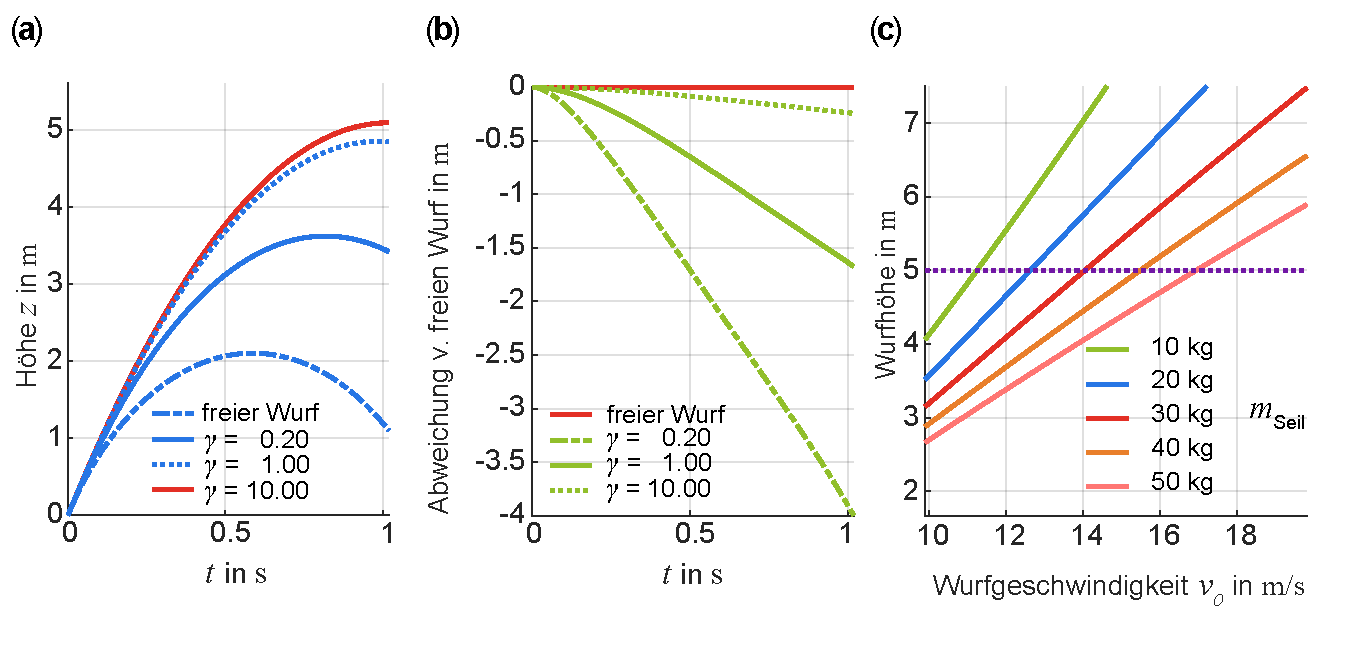
\includegraphics[width=\textwidth]{FallingChain04.pdf}
\caption[Dynamik eines Enterhakens/einer Harpune.]{Dynamik eines Enterhakens/einer Harpune. \fa Dargestellt ist die Funktion $z\lk t\rk$ f�r verschiedene Massenverh�ltnisse $\gamma = m_\text{Seil}/m_\text{K}$. Wie zu erwarten n�hert sich mit geringerer Seilmasse die Bewegung dem freien Wurf, denn wir nehmen unabh�ngig von der Gesamtmasse immer die gleiche Abwurfgeschwindigkeit an. \fb Abweichung vom freien Wurf. \fc Erreichbare Maximalh�he als Funktion der Abwurfgeschwindigkeit $v_0$ f�r verschiedene Seilmassen. Die Ankermasse (bzw. die Masse des geworfenen Tauendes ist immer $\SI{7.5}{\kg}$.}\label{abb:bew_Harpune01}
\end{figure}

Wer schon einmal am Meer beobachtet hat, wie Seeleute Taue (noch dazu nasse) beim Anlegen �ber $\approx 5$ bis $\SI{10}{\metre}$ werfen, kann nun eine Absch�tzung der Anfangsgeschwindigkeit und der dazu notwendigen Kraft machen. 
Wir wollen folgende Parameter annehmen:
	\[ m_\text{K} = \SI{7.5}{\kg} \;,~~l_\text{K} = \SI{25}{\metre}\;,~~\Delta t \approx \SI{0.2}{\s}\,,~~\Delta H = \SI{5}{\metre} \;.
	\]
Man berechnet daraus leicht Anfangsgeschwindigkeiten $v_0$ von $ \SI{11}{\metre\per\s} - \SI{18}{\metre\per\s}$ und notwendige Kr�fte $F \approx \SI{150}{\N} - \SI{650}{\N}$

\subparagraph{\textbf{Kettenfont�ne}} \index{Kettenfont�ne}

Eine besonders interessante Auspr�gung der Kettenproblematik ist die sogenannte Kettenfont�ne (\figref{bew_FallingChain01}c). Diese entsteht als Folge des nach seinem Entdecker Steve Mould\footnote{Steve Mould (geb. 1978) ist ein britischer \anf{Bildungs-Youtuber} und Wissenschaftskommunikator, der seine Wissenschaftspr�sentationen vorwiegend im Internet bringt.}\indexp{Mould, Steve} benannten Mould-Effekts, wenn eine Kette oder ein Seil aus einem Gef�� �ber den Rand nach unten gleitet. Das fallende Kettenende zieht dabei die im Gef�� liegenden Kettenglieder immer schneller nach. Der scharfe Knick, mit dem die Kette zun�chst �ber den Rand des Gef��es l�uft, weitet sich zu einem Bogen, der irgendwann den Rand nicht mehr ber�hrt, die Kette steigt zitternd in die H�he und l�st sich weiter aus dem Kn�uel. Sobald das fallende Ende den Boden erreicht, nehmen die Geschwindigkeit der Kette und damit auch die H�he der Font�ne nicht mehr weiter zu, ein station�rer Zustand ist erreicht. Im Internet sind auch zahlreiche Videos zu finden (\ua \url{https://www.youtube.com/watch?v=_dQJBBklpQQ}).\\
F�r die physikalische Erkl�rung der Entstehung des Bogens muss zus�tzlich zur Zugkraft der fallenden Kette eine weitere Kraft vorhanden sein. Diese Kraft muss aus der Energie/dem Impuls resultieren, die die Zugkraft der fallenden Kette in den Teil der Kette einbringt, der noch im Gef�� liegt \cite{Pantaleone2017}.
Die entstehende Form des Bogens l�sst sich im quasi-station�ren Zustand als eine umgekehrte Kettenlinie \index{Kettenlinie} beschreiben. Entlang dieser Kurve �ndert der Impuls kontinuierlich seine Richtung, w�hrend der Betrag (mit der L�ngsgeschwindigkeit) konstant bleibt. Die vektorielle Impuls�nderung wird gemeinsam bewirkt durch die Fallbeschleunigung einerseits und die Zugspannung in Kombination mit der Kr�mmung andererseits.\\
Wir wollen im Folgenden zun�chst ein einfaches Modell der Kettenfont�ne betrachten, welches erlaubt, die H�he der Kettenkurve �ber dem Gef�� zu berechnen und folgen hierbei der Darstellung den Autoren Biggins und Warner, die in \cite{Biggins2013, Biggins2014} erstmals eine mathematisch-physikalische Beschreibung des Ph�nomens gegeben haben.
\begin{figure}
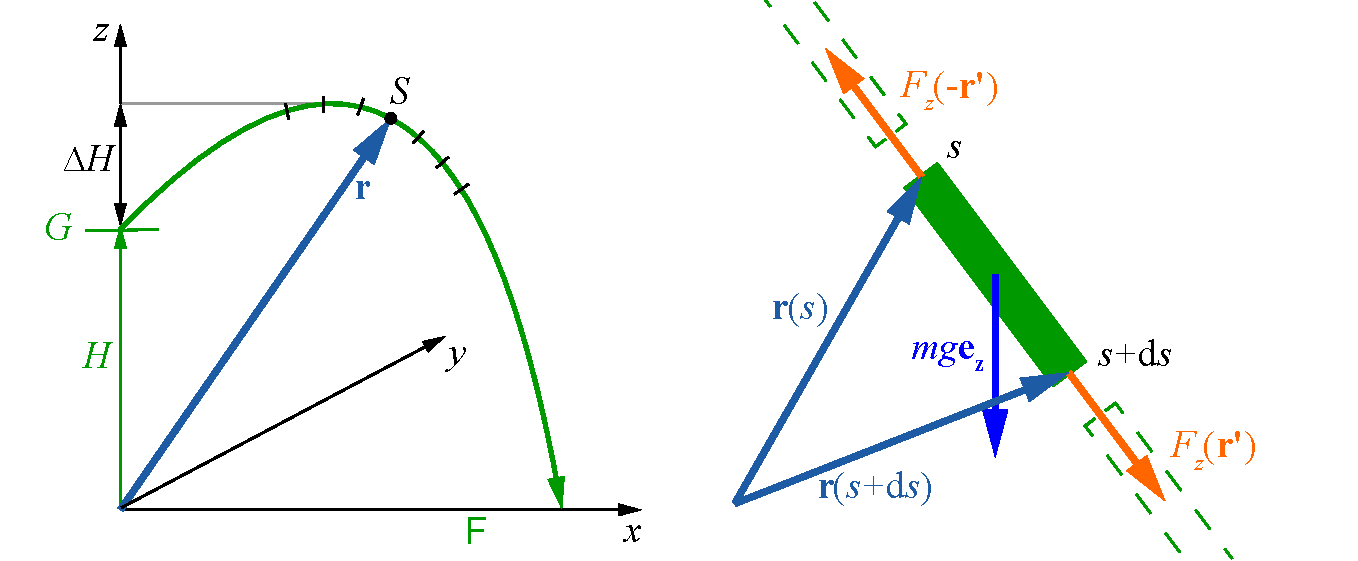
\includegraphics[width=\textwidth]{ChainFountain02.pdf}
\caption[Koordinaten und physikalische Gr��en der Kettenfont�ne.]{Koordinaten und physikalische Gr��en der Kettenfont�ne.}\label{abb:bew_chainfountain02}
\end{figure}

Wir wollen die Kette zun�chst als ein d�nnes, flexibles Seil mit konstanter L�nge annehmen.\footnote{Wir werden sp�ter sehen, dass wir zur Erkl�rung des Kettenfont�nen-Ph�nomens die Kette in diskrete Elemente \glqq zerlegen \grqq{} m�ssen.} Wir w�hlen $s$ als die L�ngengr��e entlang der Kette (\figref{bew_chainfountain02}a). Dann ist
\begin{align*}
        \vec{r}\lk s,t\rk & - \text{der Ortsvektor zur Zeit}~t~ \text{(zu einem bestimmten Punkt/Element der Kette) und} \\
        \vec{r}' = \d \vec{r}/ \d s  & - \text{der tangentiale Einheitsvektor an die Kette bei} ~ \vec{r}\lk s\rk ~\text{zur Zeit}~ t~ \\
				& \quad \text{mit} ~\vec{r}'\cdot\vec{r}' =1\,.
\end{align*} 
Wir k�nnen nun f�r ein Kettenelement $s+\D\,s$ die Newtonsche Bewegungsgleichung aufschreiben (\figref{bew_chainfountain02}b). $F_\text{Z}$ sei der Betrag der Zugkraft in der Kette (interne Spannkraft). Dann gilt:
\begin{align}
    F_\text{Z}\,\vec{r}'\big|_{s+\D s} -  F_\text{Z}\,\vec{r}'\big|_{s}  - \D m\,g\,\veceZ = \D m\,\frac{\d^2\vec{r}}{\d t^2}\,. \label{eq:bew_chainfountain01}
\end{align}
Wir f�hren die Gr��e $\mu$ als Masse pro L�nge ein ($\D m = \mu\,\D s$) und erhalten:
\begin{align}
    \frac{\d \lk F_\text{Z}\,\vec{r}'\rk}{\d s} =  \lk F_\text{Z}\,\vec{r}'\rk' = \mu\,\ddot{\vec{r}} +  \mu\,g\,\veceZ \,. \label{eq:bew_chainfountain02}
\end{align}
Der Strich bezeichnet hier eine Ableitung nach $s$. Wir wollen unter der Annahme \bzw Beobachtung, dass die Form der Font�ne zumindest f�r gewisse Zeiten relativ stabil ist, nach einer \emph{station�ren} L�sung suchen, also nach einer Kettenform $\vec{r}\lk s\rk$, die konstant in der Zeit ist, sich aber mit einer konstanten Geschwindigkeit $v$ entlang ihrer eigenen L�nge bewegen kann. Die Geschwindigkeit $v$ ist dann durch
\begin{align}
    v=\frac{\D s}{\D t} = \text{const} \label{eq:bew_chainfountain03}
\end{align}
definiert (\figref{bew_chainfountain02}c). Wir bilden:
\begin{align*}
    \vec{r}\lk t+\D\,t,s\rk &= \vec{r}\lk t,s + v\D\,t\rk \\
    \killB{\vec{r}\lk t\rk} + \frac{\d}{\d t}\vec{r}\D t + \killA{\mathcal{O}\lk \D t^2\rk} &= \killB{\vec{r}\lk t\rk} + \frac{\d}{\d s}\vec{r} \,v\D t + \killA{\mathcal{O}\lk \D t^2\rk}
\end{align*}
\begin{align}
\begin{split}
    \rightarrow ~~~~ \dot{\vec{r}} &= v \,\vec{r}'\,\\
    \rightarrow ~~~~ \ddot{\vec{r}} &= v\,\dot{\vec{r}}' = v^2\,\vec{r}''\,. 
\end{split} \label{eq:bew_chainfountain04}
\end{align}
Wir k�nnen dieses Ergebnis in \eqref{eq:bew_chainfountain02} einsetzen und erhalten:
\begin{align}
    \lk F_\text{Z}\,\vec{r}'\rk' - \mu\,g\,\veceZ = \mu\,v^2\,\vec{r}''\,. \label{eq:bew_chainfountain05}
\end{align}
Damit haben wir eine gew�hnliche DGL 2.~Ordnung f�r $\vec{r}\lk s\rk$ bekommen, die uns eine \emph{station�re} L�sung f�r die Kettenfont�ne gibt. In dieser Gleichung sind die innere Zugkraft $F_\text{Z}$ und die Geschwindigkeit $v$ noch unbekannte Parameter. Wir integrieren \eqref{eq:bew_chainfountain05} �ber $\D s$ und erhalten:
\begin{align}
    F_\text{Z}\,\vec{r}' - \mu\,g\,s\,\veceZ = \mu\,v^2\,\vec{r}' - \mu\,g\,\vec{C}\,. \label{eq:bew_chainfountain06}
\end{align}
Hierbei haben wir die Integrationskonstante $\vec{C}$ (ein Vektor!) aus im Folgenden verst�ndlichen Gr�nden mit $-\mu\,g$ multipliziert. \\
Wir formen \eqref{eq:bew_chainfountain06} um:
\begin{align}
    \lk F_\text{Z} - \mu\,v^2\rk\,\vec{r}' &= \mu\,g\,\lk s\,\veceZ-\vec{C}\rk  \nonumber \\
    \rightarrow ~~~\lk F_\text{Z} - \mu\,v^2\rk^2 &= \mu^2\,g^2\,\lk s\,\veceZ - \vec{C}\rk^2\,, \nonumber \\
    \rightarrow ~~~~ F_\text{Z} - \mu \,v^2 &= \pm\, \mu\,g\,\big| s\,\veceZ - \vec{C}\big|\,. \label{eq:bew_chainfountain07}
\end{align}
Wir multiplizieren \eqref{eq:bew_chainfountain07} mit $\vec{r}'$ und setzen $\lambda = \pm 1$:
\begin{align*}
    \lambda\,\mu\,g\,\big| s\,\veceZ - \vec{C}\big|\,\vec{r}' = \lk F_\text{Z} - \mu\,v^2\rk\,\vec{r}' = \mu\,g\,\lk s\,\veceZ - \vec{C}\rk \,,
\end{align*}
woraus
\begin{align}
  \vec{r}' = \lambda \,\frac{s\,\veceZ - \vec{C}}{\big| s\,\veceZ - \vec{C}\big|}\label{eq:bew_chainfountain08}
\end{align}
folgt. $\vec{r}'$ ist ein Einheitsvektor, was \eqref{eq:bew_chainfountain08} noch mal best�tigt. Haben wir einen Fortschritt gemacht? Schon! Wir haben eine DGL 2.Ordnung f�r $r\lk s\rk$ auf eine DGL erster Ordnung zur�ck gef�hrt und daf�r eine Integrationskonstante $\vec{C}$ (einen Vektor) erhalten, den es zu bestimmen gilt. \\
Wir vereinfachen uns das Problem etwas, indem wir annehmen, dass sich die Kettenfont�ne in der $x$-$z$-Ebene bildet. Dann kann man \eqref{eq:bew_chainfountain08} in Komponenten schreiben $\lk \vec{r} = \lk x,y,z\rk = \lk x,0,z\rk,~~ \vec{C} = \lk C_\text{x},C_\text{y},C_\text{z}\rk \rk$:
\begin{align}
    x' = \frac{\lambda\,\lk -\,C_\text{x}\rk}{\sqrt{C_\text{x}{}^2 + \lk s-C_\text{z}\rk^2}} \; , ~~~~~~~~ z' = \frac{\lambda\,\lk s-C_\text{x}\rk}{\sqrt{C_\text{x}{}^2 + \lk s-C_\text{z}\rk^2}} \label{eq:bew_chainfountain09}
\end{align}
Wir suchen ja eine L�sung f�r eine Kettenform, die einen Bogen mit �ffnung nach unten beschreibt, deswegen muss $\lambda = -1$ sein, wie man durch Bildung von $\d z'/\d s$ leicht nachrechnen kann. Die Gleichungen \eqref{eq:bew_chainfountain09} mit $\lambda = -1$ beschreiben mit $s$ als Parameter die station�re L�sung der Kettenfont�ne, allerdings noch in der Ableitung nach $s$. Wir integrieren deshalb �ber $\D s$ und erhalten:
\begin{align}
\begin{split}
    x\lk s\rk &= \ln\lek \frac{\sqrt{C_\text{x}{}^2 + \lk C_\text{z}-s\rk^2} -C_\text{z} + s}{\sqrt{C_\text{x}{}^2 + C_\text{z}{}^2} -C_\text{z}} \rek \; , \\
    z\lk s\rk &= H+ \sqrt{C_\text{x}{}^2 + C_\text{z}{}^2} - \sqrt{C_\text{x}{}^2 + \lk C_\text{z}-s\rk^2}\,,
\end{split} \label{eq:bew_chainfountain10}
\end{align}
mit den Randbedingungen  $x\lk 0\rk= 0$ und $z\lk 0\rk = H$ (H�he des Gef��bodens). \\
Wir haben jetzt mit \eqref{eq:bew_chainfountain10} die Form der Kettenfont�ne als Funktion von drei Parametern $C_\text{x}$, $C_\text{z}$ und $s$. Die beiden Gleichungen beschreiben eine Art Kettenlinie. Wir wollen nun die Parameter $C_\text{x}$, $C_\text{z}$ in Beziehung zu messbaren Gr��en setzen. \\
In \eqref{eq:bew_chainfountain07} hatten wir gefunden:
\begin{align}
    F_\text{Z} =  \mu \,v^2 \pm \mu\,g\,\big| s\,\veceZ - \vec{C}\big|\,, \label{eq:bew_chainfountain11}
\end{align}
woraus wir mit $z\lk s\rk$ aus \eqref{eq:bew_chainfountain10} f�r $\lambda = -1$
\begin{align}
    F_\text{Z}\lk s\rk = \mu\,v^2 - \mu\,g\,\lk z-H\rk - \mu\,g\,\sqrt{C_\text{x}{}^2 +C_\text{z}{}^2} \label{eq:bew_chainfountain12}
\end{align}
erhalten. Auch in dieser Darstellung $F_\text{Z}\lk z\rk$ haben wir drei unbekannte Parameter $v,C_\text{x},C_\text{z}$. Wir brauchen also Informationen �ber das System (Randbedingungen oder �hnliches), um diese freien Parameter zu bestimmen. 

\begin{figure}
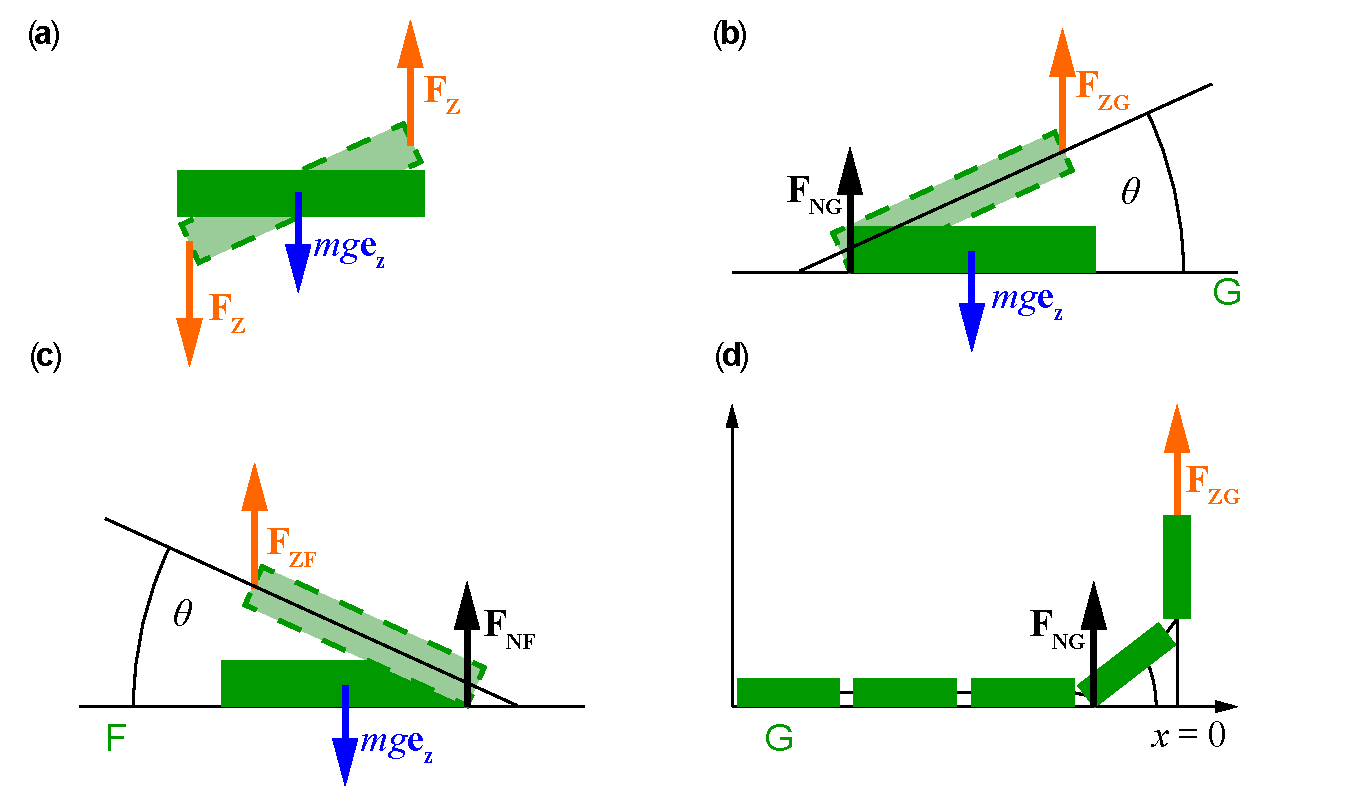
\includegraphics[width=\textwidth]{ChainFountain02a.pdf}
\caption[Kr�fte an den Kettengliedern einer Kettenfont�ne.]{Kr�fte an den Kettengliedern einer Kettenfont�ne. \fa Ein Kettenglied, das nicht auf einer Unterlage aufliegt, wird sich um seinen Schwerpunkt drehen. \fb Kr�fte bei einem abhebenden Kettenglied auf dem Gef��boden. \fc Kr�fte bei einem auftreffenden Kettenglied auf dem Fu�boden. \fd Winkel beim Abheben eines Kettengliedes.} \label{abb:bew_chainfountain02a}
\end{figure}

An dieser Stelle m�ssen wir nun das einfache Modell des Seil verlassen und ein Modell der Kette mit diskreten, als stabf�rmig angenommenen Kettengliedern benutzen. Wir betrachten \figref{bew_chainfountain02a}b und schreiben zun�chst die Newtonsche Bewegungsgleichung f�r ein einzelnes Kettenglied auf, das sich in der N�he des Gef��bodens (G)
befindet:
\begin{align*}
    F_\text{N,G} = m\,g + F_\text{Z,G} = \mu\,l_\text{K}\,\frac{\Delta v}{l_\text{K}/\Delta v} \approx \mu\,v^2 \,.
\end{align*}
Hier ist $F_\text{N,G}$ eine Normalkraft des Gef��bodens und $F_\text{Z,G}$ die wirkende Zugkraft in dem Kettenglied, das sich gerade vom Boden des Gef��es l�st. Da f�r ein einzelnes Kettenglied $m\,g = \mu\,l_\text{K}\,g$ sehr klein ist, k�nnen wir n�herungsweise schreiben
\begin{align}
    F_\text{Z,G} + F_\text{N,G} \approx \mu\,v^2 \label{eq:bew_chainfountain13a}
\end{align}
und analog f�r den Fu�boden (F):
\begin{align}
     F_\text{Z,F} +  F_\text{N,F} \approx \mu\,v^2 \,. \label{eq:bew_chainfountain13b} 
\end{align}
In \eqref{eq:bew_chainfountain13a} und \eqref{eq:bew_chainfountain13b} sind:
	\[	F_\text{Z,G} =  F_\text{Z}\lk H\rk ~~~~ \text{und} ~~~~  F_\text{Z,F} =  F_\text{Z}\lk 0\rk\,.\]
Wir setzen nun \eqref{eq:bew_chainfountain12} in \eqref{eq:bew_chainfountain13a} ein und erhalten
\begin{align*}
    -\mu\,g\,\sqrt{C_\text{x}{}^2 +C_\text{z}{}^2} + F_\text{N,G} = 0\,,\\
    -\mu\,g\,H - \mu\,g\,\sqrt{C_\text{x}{}^2 +C_\text{z}{}^2} + F_\text{N,F} = 0\,,
\end{align*}
woraus folgt $F_\text{N,G}>0$. \\
Warum �bt der Boden des Gef��es eine Normalkraft in positive $z$-Richtung auf die Kette aus? Das erscheint zun�chst paradox. F�r den Moment des Abhebens schauen wir uns die Newtonsche Bewegungsgleichung f�r die $z$- und die $\theta$-Koordinate genauer an\footnote{Die Gleichung f�r die $\theta$-Koordinate entspricht der Drehmomentbilanz (\kap{bew_Drehimpuls_StarrerK}).} (\figref{bew_chainfountain02a}b):
\begin{align}
\begin{split}
    F_\text{N,G} + F_\text{Z,G} -m\,g &= m\,\ddot{z}\,, \\
    F_\text{Z,G} \,\frac{l_\text{K}}{2}\,\cos\theta - F_\text{N,G}\,\frac{l_\text{K}}{2}\,\cos\theta &= J\,\ddot{\theta}\,. \label{eq:bew_chainfountain14}
\end{split}
\end{align}
Hierin ist $J$ das Tr�gheitsmoment des Kettengliedes bez�glich seines Schwerpunktes (\kap{bew_Drehimpuls_StarrerK}).
DGL-System \eqref{eq:bew_chainfountain14} kann numerisch gel�st werden.
Wir wollen uns aber vorerst die lineare N�herung f�r kleine Winkel anschauen, wohl wissend, dass $\theta$ auch gro�e Werte annehmen kann. Wir werden diese N�herung deshalb auch gleich wieder fallen lassen, k�nnen aber zun�chst mit $\cos\theta \approx 0$ und $z\approx (l_\text{K}\,\theta )/ 2$ schreiben:
\begin{align}
\begin{split}
    F_\text{Z,G} + F_\text{N,G}  - m\,g &= m\,\ddot{z} \approx m\,\frac{v^2}{l_\text{K}}\,,\\
    \frac{l_\text{K}}{2}\,F_\text{Z,G} - F_\text{N,G} \,\frac{l_\text{K}}{2} &= 2J\,\ddot{\theta}\,. \label{eq:bew_chainfountain15}
\end{split}
\end{align}
Wir k�nnen nun aus \eqref{eq:bew_chainfountain15} $F_\text{Z,G}$ eliminieren und erhalten mit $J=\frac{1}{12}\,m\,l_\text{K}^2$ f�r einen homogenen Stab und $m\,g \ll F_\text{Z,G},F_\text{N,G}  $:
\begin{align}
    F_\text{N,G} = \frac{1}{2}\,\lk m-\frac{4J}{l_\text{K}^2}\rk\,\frac{v^2}{l_\text{K}} = \frac{1}{3}\,m\,\frac{v^2}{l_\text{K}} = \frac{1}{3}\,\mu\,v^2 \,.  \label{eq:bew_chainfountain16}
\end{align}
Wir erinnern uns, dass $F_\text{N,G}$ nach \eqref{eq:bew_chainfountain16} der Bedingung kleine Winkel hergeleitet wurde, deswegen schreiben wir zur Ber�cksichtigung gr��erer Winkel besser verallgemeinert
\begin{align}
    F_\text{N,G} = \alpha \,\mu\,v^2 \,, \label{eq:bew_chainfountain17}
\end{align}
worin $\alpha$ eine gegebenenfalls numerisch oder experimentell zu bestimmende Konstante des Systems ist.\footnote{Die Proportionalit�t ist eine Annahme, die durch das Experiment verifiziert werden kann.} \\
V�llig analog kann man die Situation beim Auftreffen auf dem Fu�boden beschreiben und wir finden dann f�r die entsprechende Normalkraft (\figref{bew_chainfountain02a}c):
\begin{align}
    F_\text{N,F} = \lk 1-\beta\rk\,\mu\,v^2 \,,\label{eq:bew_chainfountain18}
\end{align}
worin $\beta$ wieder eine experimentell bzw. numerisch zu bestimmende Konstante ist. Experimentell findet man Werte von $\alpha\approx\SI{0.12}{}$ und $\beta \leq \SI{0.1}{}$. 
Damit k�nnen wir nun auch die Zugkr�fte in der Kette im Gef�� und auf dem Fu�boden bestimmen:
\begin{align}
\begin{split}
    F_\text{Z,G} &= \mu\,g\,\sqrt{C_\text{x}{}^2 +C_\text{z}{}^2} = \alpha\,\mu\,v^2     \,,   \\
    F_\text{Z,F} &= \mu\,g\,\sqrt{C_\text{x}{}^2 +C_\text{z}{}^2} + \mu\,g\,H = \lk 1-\beta\rk\,\mu\,v^2\,. \label{eq:bew_chainfountain19}
\end{split}
\end{align}
Da $\alpha$ und $\beta$ jetzt bekannt \bzw experimentell bestimmt sind, bleibt $v$ als einzige Unbekannte. Diese k�nnen wir aus \eqref{eq:bew_chainfountain19} erhalten:
\begin{align}
   \killA{\mu}\,g\,H &= \lk 1-\alpha-\beta\rk\,\killA{\mu}\,v^2 ~~\rightarrow ~~ v = \sqrt{\frac{g\,H}{\lk 1-\alpha-\beta\rk}}\approx \sqrt{\frac{g\,H}{0.77}} \label{eq:bew_chainfountain20}
\end{align}
Entscheidend f�r die Entstehung einer Kettenfont�ne ist der Abstand zwischen Kettengliedern \bzw die L�nge der Verbindungsst�cken, die in jedem Fall so klein sein muss, dass das gerade abhebende Kettenglied beim Abheben nicht unter dem Winkel von $90\degree$ abheben kann. Interessant ist auch, dass die Fallgeschwindigkeit der Kettenfont�ne geringer ist als die Geschwindigkeit des freien Falls $\sqrt{2\,g\,H}$, was offensichtlich durch die wirkenden Normalkr�fte von Gef��- und Fu�boden zustande kommt. Wir kommen darauf noch einmal zur�ck. Setzen wir $v$ in die ersten Gleichung von \eqref{eq:bew_chainfountain19} ein, erhalten wir daraus eine Beziehung zwischen den Konstanten $C_\text{x}$ und $C_\text{z}$:
\begin{align}
    C_\text{x} = +\sqrt{\lek \frac{\alpha\,H}{\lk 1-\alpha-\beta\rk}\rek^2-C_\text{z}{}^2}\,. \label{eq:bew_chainfountain21}
\end{align}
Setzen wir diese in \eqref{eq:bew_chainfountain12} ein, finden wir f�r die Zugkraft:
\begin{align}
    F_\text{Z}\lk z\rk = \lambda\,g\,\lek z + \frac{\beta\,H}{1-\alpha-\beta}\rek = \lambda\,g\,\lek z + \frac{\beta \, \gamma}{\alpha}\rek ~~\text{mit}~~\gamma= \frac{\alpha\,H}{1-\alpha-\beta}\,.\label{eq:bew_chainfountain22}
\end{align}
Damit haben wir unser Ziel erreicht, und die Zugkraft $F_\text{Z}\lk z\rk$ als Funktion von bekannten geometrischen und physikalischen Parametern und der H�he $z$ �ber dem Fu�boden beschrieben. Damit k�nnen wir auch die Gleichungen der Kettenlinie in Parameterform von $s$, $\alpha$ und $\beta$ \bzw $\gamma$ schreiben:
%\begin{align*}
%\begin{split}
    %x\lk s\rk &= \sqrt{\lk \frac{\alpha\,H}{\lk 1-\alpha-\beta\rk}\rk^2 -C_\text{z}{}^2}\,\ln\lek\frac{\sqrt{\lk \frac{\alpha\,H}{\lk 1-\alpha-\beta\rk}\rk^2-2C_\text{z}\,s+s^2} - C_\text{z} + s}{\frac{\alpha\,H}{\lk 1-\alpha-\beta\rk} - C_\text{z}}\rek\,, \\
    %z\lk s\rk &= H + \frac{\alpha\,H}{\lk 1-\alpha-\beta\rk} - \sqrt{\lek \frac{\alpha\,H}{\lk 1-\alpha-\beta\rk}\rek^2 - 2C_\text{z}\,s + s^2} \,.
%\end{split} 
%\end{align*}
\begin{align}
\begin{split}
    x\lk s\rk &= \sqrt{\gamma^2 - C_\text{z}{}^2}\,\ln\lek\frac{\sqrt{\gamma^2-2C_\text{z}\,s+s^2} - C_\text{z} + s}{\gamma - C_\text{z}}\rek\,, \\
    z\lk s\rk &= H + \gamma - \sqrt{\gamma^2 - 2C_\text{z}\,s + s^2} \,.
\end{split} \label{eq:bew_chainfountain23}
\end{align}
Leider haben wir in diesen parametrisierten Gleichungen noch immer eine Unbekannte ($C_\text{z}$).
Wir brauchen also noch eine weitere Bedingung, um diese zu bestimmen 
und betrachten dazu einen Grenzfall f�r einen Impulseintrag aus dem Gef��,
n�mlich wenn das Kettenglied im Moment des Abhebens (\figref{bew_chainfountain02a}d) nahezu senkrecht steht. Dann m�sste gelten:
	\[z' = \frac{\d z}{\d s} \big|_0 \approx 1 ~~ \text{und}~~ x' = \frac{\d x}{\d s}\big|_0 \approx 0\,. \]
Setzen wir diese Grenzbedingungen in \eqref{eq:bew_chainfountain23} ein, k�nnen wir das noch fehlende Glied $C_\text{z}$ bestimmen und erhalten damit:
\begin{align}
\begin{split}
    C_\text{x} &= \gamma\, \\
    \rightarrow ~~ x\lk s\rk &= 0 \,~ \text{und} ~
    z\lk s\rk = \frac{\lk 1-\beta\rk\,H}{\lk 1-\alpha-\beta\rk} - \Bigg| \frac{\alpha\,H}{\lk 1-\alpha-\beta\rk} -s\Bigg| = \frac{1-\beta}{\alpha}\,\gamma - \Bigg| \gamma -s\Bigg| \,.
\end{split} \label{eq:bew_chainfountain24}
\end{align}
Offensichtlich beschreibt diese station�re L�sung eine in sich zur�cklaufende Kette, die bei $z_{\max} > H$ einen h�chsten Punkt erreicht:
\begin{align}
    z_{\max} &= \frac{\lk 1-\beta\rk\,H}{\lk 1-\alpha-\beta\rk} ~~\rightarrow ~~\Delta H &= z_{\max} - H = \frac{\alpha\,H}{\lk 1-\alpha-\beta\rk} \,.
\label{eq:bew_chainfountain25}
\end{align}
\figref{bew_chainfountain04}a zeigt berechnete Werte f�r $z_{\max}$ f�r verschiedene Parameter. Die Font�nenh�he $\Delta H$ h�ngt also von der Gef��h�he $H$ und dem Parameter $\alpha$ ab, weniger von $\beta$. Das ist nicht �berraschend, da die Font�nenh�he vom Impuls abh�ngt, der von der Unterlage auf die Kette �bertragen wird. Dieser h�ngt aber wiederum von der Geschwindigkeit der Kette ab, die aber als Wirkung aus der Gravitation von der H�he $H$ abh�ngt \eqref{eq:bew_chainfountain20}.\\
Offensichtlich folgt f�r $\alpha = 0,\, \beta = 0$ und $\Delta H=0$ dann $v^2 = H\,g$. Das ist der Fall einer frei fallenden Kette der L�nge $H$, den wir schon in \eqref{eq:bew_FallingChain05} berechnet hatten.\\
Nat�rlich kann in der Realit�t eine Kette nicht in sich (bei $x=0$) zur�ck laufen. Das �berraschende Ergebnis unseres Modells ist in zwei gemachten Annahmen begr�ndet. Zum einen hatten wir den Grenzfall $z' = \d z/\d s (0) \approx 1 $ angenommen und zum anderen stillschweigend eine unendlich d�nne Kette angenommen, bei der alle Kettenglieder bei $x=0$ vom Boden des Gef��es abheben. Beides sind in der Realit�t sicher nicht zutreffende Annahmen. Unser Modell liefert aber dennoch sehr realistische H�hen der Font�ne �ber dem Gef��.\\

Wir wollen zum Schluss noch die energetischen Verh�ltnisse und den Radius des Bogens der Kettenfont�ne betrachten. F�r das Verh�ltnis von kinetischer Energie der Kette zu potentieller Energie (pro L�ngeneinheit) finden wir:
\begin{align}
    \frac{T}{U} &= \frac{v^2/2}{g\,H} = \frac{1}{2}\frac{1}{ 1-\alpha-\beta}\,.
\label{eq:bew_chainfountain26}
\end{align}
Wiederum ergibt sich f�r $\alpha=\beta=0$ der Fall der frei fallenden Kette mit einem Energieverh�ltnis von 0.5 bei der Kettenfont�ne interessanterweise etwas weniger. Aus \eqref{eq:bew_chainfountain26} folgt auch, dass $\alpha+\beta \leq 0.5$ sein muss. 
%Bei $\alpha = 0.5$ und $\beta=0$ w�rde $\Delta H = H$ folgen und es g�be keine Energiedissipation. Das ist aber unrealistisch, weil die Parameter $\alpha$ und $\beta$ von vergleichbarer Gr��e sind (zur Berechnung von $\alpha$ siehe auch \cite{Biggins2013}).
Der sich ausbildende Bogen der Kette kann nur durch die Wirkung der Zugkraft als Radialkraft zustande kommen (wir nehmen wieder an $F_\text{Z,B} \gg m\,g$). Dann muss gelten (\figref{bew_FallingChain01}c):
\begin{align}
    \frac{F_\text{Z,B}}{R} &= \frac{\mu\,v^2}{R} \,.
\label{eq:bew_chainfountain27}
\end{align}
Interessanterweise k�rzt sich der Radius des Bogens heraus, was bedeutet, dass solange $v^2 \gg g\, R$ gilt es auch sehr, sehr enge Kurvenradien geben kann. Dies rechtfertigt nachtr�glich unsere Modellannahmen, bedeutet aber auch, dass das Modell keine Erkl�rung f�r den Radius des Bogens der Font�ne liefern kann. F�r weitergehende Betrachtungen empfehlen wir \cite{Biggins2013, Biggins2014, Pantaleone2017, Anghel2021}. \\

\begin{figure}
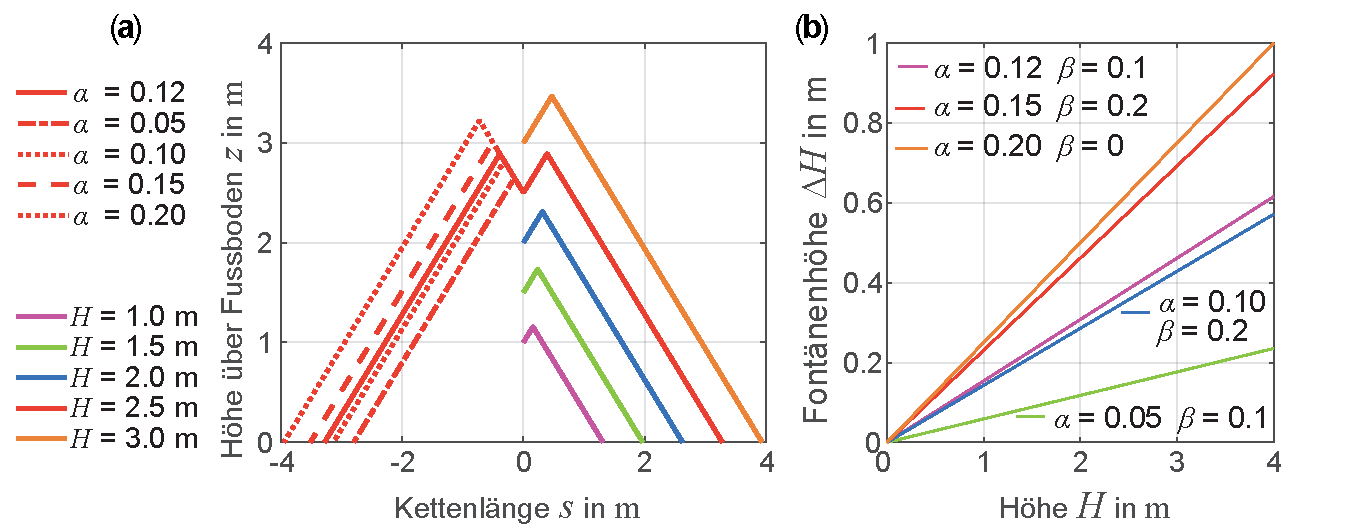
\includegraphics[width=\textwidth]{ChainFountain03.pdf}
\caption[H�he der Kettenfont�ne. ]{H�he der Kettenfont�ne �ber der Kettenl�nge $s$ als Funktion der Parameter $\alpha, \beta$ und $H$. Man beachte, dass im linken Bild $s$ keine kartesische Koordinate ist, sondern die L�nge entlang der Kette. $H$ ist die H�he des Gef��es �ber den Fu�boden.}\label{abb:bew_chainfountain04}
\end{figure}
Wir wollten mit diesem Kapitel zeigen, 
\begin{enumerate}
    \item [a)]
    dass man zur Beschreibung eines physikalischen Problems unter Umst�nden mehrere, z.T. sehr unterschiedliche Modelle braucht (in unserem Fall Kontinuum (Seil) und diskrete Elemente der Kette)
    \item [b)]
    dass es Sinn macht, auch bei einem dynamischen Problem nach einer quasi-station�ren L�sung zu suchen, 
    \item [c)]
    dass man alle denkbaren Rand- und Nebenbedingungen untersuchen muss, um Konstanten der Bewegung zu bestimmen, und
    %\item [e)]
    %dass es Systeme aus Massepunkten gibt, die obwohl es keinen Reibungsterm in den Bewegungsgleichungen gibt, zu Energiedissipation f�hren k�nnen, und  
    \item [d)]
    dass man die Wirkung von Normalkr�ften auf einen ausgedehnten K�rper nicht untersch�tzen darf.%
    \footnote{Wir werden entsprechende Effekte auch in \kap{bew_fallendeLeiter} wieder finden und auch n�her betrachten.}
\end{enumerate}


\clearpage
\section{Mechanik starrer K�rper}\label{kap:bew_starrer_koerper}
\index{K�rper!starrer}

Die vorherigen Abschnitte betrachteten nur Situationen, in denen ein K�rper
als Punktmasse behandelt werden konnte.
In vielen Anwendungen greift diese N�herung jedoch
zu kurz und muss die Ausdehnung des K�rpers explizit einbezogen
werden.
Das wollen wir in diesem Kapitel tun und dabei annehmen, dass
der K�rper w�hrend der gesamten Bewegung seine Form beh�lt, also nicht
deformierbar ist. 
Dies ist das Modell des starren K�rpers.

Ein starrer K�rper kann \zb aus einem System von $N$ diskreten Massepunkten
bestehen.
Dies haben wir bereits in \ref{kap:bew_basics_of_systems} betrachtet, sodass wir darauf Bezug nehmen k�nnen.
In den meisten F�llen l�sst sich ein starrer K�rper jedoch als eine kontinuierliche
Massenverteilung mit der Dichte $\varrho(\vec{r})$ betrachten, sodass wir das Konzept entsprechend erweitern.
Die
Gesamtmasse des K�rpers betr�gt dann
\begin{equation}
  M = \int_V \varrho(\vec{r}) \, \D^3 r  ~,
\end{equation}
wobei �ber sein gesamtes Volumen $V$ integriert wird.

Da der K�rper seine Gestalt nicht ver�ndert, ist es sinnvoll, zu seiner
Beschreibung zwei Koordinatensysteme einzuf�hren, ein raumfestes KOS $\vec{\Sigma}$ mit
den Standardachsen $\veceX$, $\veceY$ und $\veceZ$ und ein
k�rperfestes KOS $\vec{\Sigma}'$, dessen Achsen wir mit $\vecpeX$, $\vecpeY$ und
$\vecpeZ$ bezeichnen wollen und das seinen Ursprung im Schwerpunkt des
K�rpers hat (siehe \figref{bew_KOS_starrerKoerper}).

\begin{figure}
  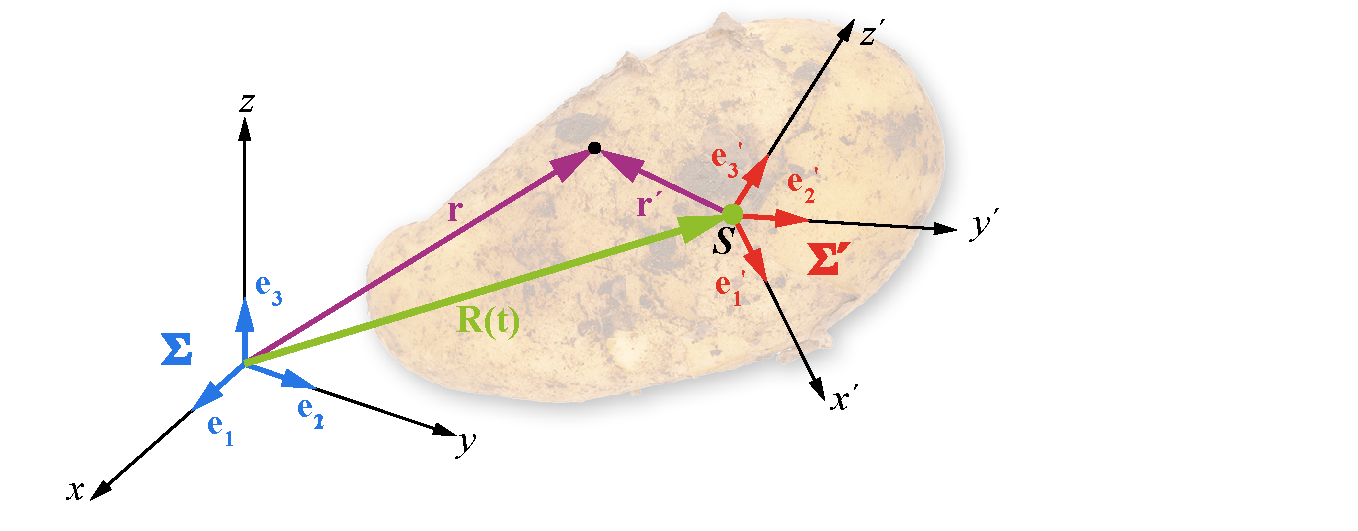
\includegraphics[width=\textwidth]{StarrKoerpKOS.pdf}
  \caption[Koordinatensysteme des starren K�rpers.]{Zur Beschreibung eines
    starren K�rpers ist es sinnvoll, ein raumfestes Koordinatensystem \index{Koordinatensystem!raumfestes} mit
    den Standardachsen  $\veceX$, $\veceY$ und $\veceZ$ sowie
    ein k�rperfestes\index{Koordinatensystem!k�rperfestes} mit den Achsen $\vecpeX$, $\vecpeY$ und
    $\vecpeZ$ heranzuziehen. Das k�rperfeste System hat seinen Ursprung
    im Schwerpunkt des K�rpers.}
    \label{abb:bew_KOS_starrerKoerper}
\end{figure}

Einen Vektor zu einem Punkt des K�rpers k�nnen wir somit im Koordinatensystem
$\vec{\Sigma}$ aus dem Schwerpunktsvektor $\vec{R}_S$ und einem Vektor $\vec{r'}$
aus dem k�rperfesten System $\vec{\Sigma}'$ mithilfe der entsprechenden Koordinatentransformation
zusammensetzen (siehe auch \kap{bew_rotating_systems}):
\begin{equation}
  \vec{r} = \vec{R}_S + \mathbb{R} \vec{r}' \,.
\end{equation}
Der Vektor $\vec{r}'$ zeigt vom Schwerpunkt zum Punkt im K�rper. 
Da er im k�rperfesten System gegeben ist, h�ngen seine Koordinaten nicht von der Zeit ab. Wir bezeichnen ihn im Folgenden mit $\vec{x}'$, um eine Verwechslung mit der Darstellung von $\vec{r}$ im k�rperfesten System $\vec{\Sigma}'$ zu vermeiden. Seine Darstellung im raumfesten System $\vec{\Sigma}$ nennen wir $\vec{x}$.


F�r die Geschwindigkeit dieses Punktes im raumfesten KOS folgt analog zu \kap{bew_rotating_systems}
\begin{equation}
  \vec{v} = \frac{\D}{\D t} \vec{r} = \vec{V}_S + \vec{\omega}' \times \vec{r}' = \vec{V}_S + \vec{\omega} \times \vec{x} \,,
  \label{eq:bew_Geschw_starrerK}
\end{equation}
mit der Schwerpunktgeschwindigkeit $\vec{V}_S$ und der momentanen Winkelgeschwindigkeit
$\vec{\omega}(t)$ der Drehbewegung des k�rperfesten Bezugssystems.

\subsection{Grundlagen der Kinematik}\index{Tr�gheitstensor}\index{Tr�gheitsmoment} \label{kap:bew_Kinematik_StarrerK}

\subsubsection{Kinetische Energie, Tr�gheitstensor und Tr�gheitsmoment}
\label{kap:bew_StarrerK_kin_Energie}

Die kinetische Energie eines starren K�rpers berechnet sich entsprechend Definition \eqref{eq:bew_Ges_Energie} unter Nutzung der Beziehung f�r die 
Geschwindigkeit \eqref{eq:bew_Geschw_starrerK} zu
\begin{align}
  T &= \frac{1}{2} \int_V \varrho(\vec{x}) \left ( \vec{V}_S
      + \vec{\omega} \times \vec{x} \right )^2 \, \D^3 x
      = \frac{1}{2} \int_V \varrho(\vec{x}) \left ( {\vec{V}_S}^2
      + (\vec{\omega} \times \vec{x})^2 \right ) \, \D^3 x \\
    &= \frac{1}{2} M\,{\vec{V}_S}^2 + \frac{1}{2} \int_V \varrho(\vec{x})
      (\vec{\omega} \times \vec{x})^2 \, \D^3 x
    = T_\mathrm{trans} + T_\mathrm{rot}\,.
      \label{eq:bew_Kin_Energie_starrerK}
\end{align}
Die kinetische Energie setzt sich aus einem Term $T_\mathrm{trans}$, der aus der Translation des Schwerpunkts
stammt, und der Rotationsenergie $T_\mathrm{rot}$ zusammen.
Der Mischterm aus dem ersten
Integral verschwindet, da in diesem $\vec{x}$ linear vorkommt und somit das Integral den
Schwerpunkt berechnet, der aber gerade den Wert $\vec{x} = \vec{0}$ hat.%
\footnote{Es gilt ja 
	$\int_V \varrho(\vec{x})\, \vec{x} \,\D^3 x = \vec{0}$.}

Die Rotationsenergie l�sst sich noch so umschreiben, dass wir die Eigenschaft
des K�rpers (seine Massenverteilung) von der Drehachse und der Winkelgeschwindigkeit trennen k�nnen.\footnote{$M$ bezeichnet hier die Gesamtmasse des starren K�rpers und man muss en bisschen aufpassen, dass man diese nicht mit dem Betrag des Drehmoments verwechselt, das wir \ia mit $\vec{M}_\text{D}$ bezeichnen. Wir werden auch bei den Beispielen zur besseren Eindeutigkeit die Massen h�ufig mit $m$ bezeichnen.}
Mit der Rechenregel $(\vec{a} \times \vec{b})^2 = \vec{a}^2 \vec{b}^2 - (\vec{a}\cdot \vec{b)^2}$ der Vektoralgebra (siehe die \onlineZ) folgt
\begin{equation}
  T_\mathrm{rot} = \frac{1}{2} \vec{\omega}^T \,\underline{\vec{\Theta}} \,\vec{\omega} = \frac{1}{2} \lk\omega_1\,,\omega_2\,,\omega_3\rk \,\underline{\vec{\Theta}} \,\lk\begin{array} {l} \omega_1\\\omega_2\\ \omega_3\end{array}\rk\,,
  \label{eq:bew_Trot_starrerK}
\end{equation}
worin $\underline{\vec{\Theta}}$ der \emph{Tr�gheitstensor}\footnote{%
In der linearen Algebra ist der Begriff des Tensors\index{Tensor} eine Verallgemeinerung des Begriffs der Matrix. 
Da wir hier keine weitergehende Theorie f�r Tensoren ben�tigen, k�nnen wir f�r unsere Zwecke die Begriffe Tensor und Matrix synonym verwenden. Zur Kennzeichnung eines Tensor benutzen wir \ia als Symbol einen unterstrichenen Vektor $\underline{\vec{A}}$ oder $\mathbb{A}$.  
F�r tiefergehende Betrachtungen sei auf \cite{Riley2006, Felder2016, Bartelmann2015} und \cite{Otto2019, Fischer2018} verwiesen.}
ist, der die Eigenschaften des K�rpers enth�lt und dessen Komponenten
\begin{subequations}
  \begin{align}
    \Theta_{ij} &= \int_V \varrho(\vec{x}) \left ( \vec{x}^2 \delta_{ij} -x_i x_j
    \right )\, \D^3 x  \\
    \intertext{\bzw ausgeschrieben}
    \underline{\vec{\Theta}} &= \begin{pmatrix} \Theta_{11}&\Theta_{12}&\Theta_{13}\\ \Theta_{21}&\Theta_{22}&\Theta_{23}\\ \Theta_{31}&\Theta_{32}&\Theta_{33}
    \end{pmatrix}
     = \bigintsss_V \varrho(\vec{x}) \begin{pmatrix} y^2+z^2 & -x\,y & -x\,z \\ -x\,y & x^2+z^2 & -y\,z \\ -x\,z & -y\,z & x^2+y^2 \end{pmatrix} \, \D^3 x \label{eq:bew_traegheitstensor}
  \end{align}
\end{subequations}
lauten. $\delta_{ij}$ ist das Kronecker-Symbol\index{Kronecker-Symbol}\indexp{Kronecker, Leopold}. Ist der Tr�gheitstensor bekannt, kann f�r jede Drehung des K�rpers\index{Drehung} die kinetische
Energie mit dieser quadratischen Form und der vektoriellen
Winkelgeschwindigkeit $\vec{\omega}$ berechnet werden.
Der Tr�gheitstensor ist eine physikalische Gr��e f�r die Masseverteilung eines
starren K�rpers und spielt damit bei 
Rotationen die Rolle der tr�gen Masse, die der K�rper bei Translationsbewegungen hat. 
Da der Tr�gheitstensor $\underline{\vec{\Theta}}$ symmetrisch ist, hat er nur sechs unabh�ngige Elemente, seine Diagonalelement hei�en \emph{Tr�gheitsmomente}\index{Tr�gheitsmomente}.

In den meisten Anwendungen wird
die Drehachse fest vorgegeben sein.
Dann ist es unn�tig den gesamten
Tr�gheitstensor zu kennen.
Wir ben�tigen nur das Verhalten des K�rpers
f�r die Drehung um eine einzige Achse.
Dazu stellen wir die vektorielle
Winkelgeschwindigkeit $\vec{\omega}$ als Produkt eines Einheitsvektors $\vec{n}_\omega$,
der die Richtung der Drehachse beschreibt, und ihres Betrags $\omega$ dar.
Damit erhalten wir f�r das quadrierte Kreuzprodukt in der Rotationsenergie
aus \eqref{eq:bew_Kin_Energie_starrerK}
\begin{equation*}
  \left ( \vec{\omega} \times \vec{x} \right )^2 =  \omega^2 \left
    ( \vec{n_\omega} \times \vec{x} \right )^2 = \omega^2 {x_\perp}^2
\end{equation*}
mit dem Anteil $x_\perp$ des Vektors $\vec{x}$, der senkrecht zur
Drehachse steht.
F�r die Rotationsenergie ergibt sich
\begin{equation}
  T_\mathrm{rot} = \frac{1}{2} \omega^2 \int_V \varrho(\vec{x})\, {x_\perp}^2
 \, \D^3 x = \frac{1}{2} \,J \,\omega^2
\end{equation}
mit dem Tr�gheitsmoment $J$
\begin{equation}
  J = \vec{\Theta}_{\,\vec{n_\omega}} = \int_V \varrho(\vec{x})\, {x_\perp}^2 \,\D^3 x ~ ,
\end{equation}
das f�r die gew�hlte Drehachse $\vec{n_\omega}$ gilt.\\
Da $\underline{\vec{\Theta}}$ symmetrisch ist, hat $\underline{\vec{\Theta}}$ drei reelle Eigenwerte mit
zueinander paarweise senkrechten Eigenvektoren.
Diese Eigenwerte $\Theta_1\,, \Theta_2\,, \Theta_3$ hei�en \emph{Haupttr�gheitsmomente}\index{Haupttr�gheitsmomente},
die wir fortan mit $J_1\,, J_2\,, J_3$ bezeichnen wollen,
die Richtungen der Eigenvektoren hei�en Haupttr�gheitsachsen.
Wir k�nnen diese als Koordinatenachsen des k�rperfesten Systems $\vec{\Sigma}'$ vereinbaren.
Dann nimmt $\underline{\vec{\Theta}}'$ (also der Tr�gheitstensor $\underline{\vec{\Theta}}$ ausgedr�ckt in seinen Komponenten im k�rperfesten System $\vec{\Sigma}'$) eine einfache Diagonalform an\footnote{Da die Angabe des Haupttr�gheitssysems nur im k�rperfesten KOS $\vec{\Sigma}'$ sinnvoll ist, verwenden wir $\vec{J}$ nur in diesem und verzichten hier auf die Angabe eines Striches und Unterstriches als Tensor, da wir die Diagonalelemente $\Theta_{ii}$ als Komponenten $J_1, J_2, J_3$ eines Vektors $\vec{J}$ betrachten k�nnen.
Die Diagonalmatrix $\vec{J}$ oder ihre Komponenten beziehen sich immer auf $\vec{\Sigma}'$.}:
\begin{equation}
\lk \begin{array} {lll} \Theta_{11}&0&0\\ 0&\Theta_{22}&0\\ 0&0&\Theta_{33}
            \end{array}\rk = \lk \begin{array} {lll} J_{1}&0&0\\ 0&J_{2}&0\\ 0&0&J_{3} \end{array}\rk\, = \lk \begin{array} {lll} J_x&0&0\\ 0&J_y&0\\ 0&0&J_z \end{array} \rk \,\widehat{=}  \,
\lk \begin{array} {l} J_{1}\\ J_{2}\\ J_{3} \end{array} \rk \,=\,\vec{J}\,. \label{eq:bew_traegheitsmoment}
\end{equation}
Die Tr�gheitsmomente eines starren K�rpers findet man, indem man zun�chst den Tr�gheitstensor nach \eqref{eq:bew_traegheitstensor} berechnet und dann f�r diesen das Eigenwertproblem 
\begin{equation}
  \underline{\vec{\Theta}} \, \vec{n}_{\omega_i} = J_i \, \vec{n}_{\omega_i}
\end{equation}
l�st und gegebenenfalls die Hauptachsen $\vec{n}_{\omega_i}$ mit $i = 1,2,3$ bestimmt.
Falls mehrere Tr�gheitsmomente (Eigenwerte) gleich sind, m�ssen die entsprechenden Eigenvektoren so
gew�hlt werden, dass alle paarweise orthogonal sind. \\
Bei K�rpern mit Symmetrieachsen\index{Symmetrieachsen} l�ngs der Koordinatenachsen des k�rperfesten Systems ist der Tr�gheits\-tensor automatisch diagonal.
Die Symmetrieachsen stellen genau die Haupttr�gheitsachsen\index{Haupttr�gheitsachsen} dar, siehe dazu das folgende Beispiel und \probref{bew_traegheitsmomente}, in der wir Tr�gheitsmomente verschiedener K�rper berechnen.

%BEISPIEL %%%%%%%%%%%%%%%%%%%%%%%%%%%%%%%%%%%%%%%%%%%%%%%%%%%%%%%%%%%%%%%%%%%%%%%%%%%%%%%%%%
\begin{example}{Tr�gheitstensor eines Quaders}
\label{bsp:bew_Traegheitstensor}
\smallskip

Wir berechnen den Tr�gheitstensor f�r einen Quader mit den Kantenl�ngen $a$,
$b$ und $c$ und der homogenen Massendichte $\varrho = M/V = M/(abc)$, der sich
um Achsen durch seinen Schwerpunkt dreht.
Die Achsen sind dabei parallel zu den
Kanten gew�hlt.
Wir f�hren das Koordinatensystem wie in \figref{bew_TraegTensorQuad}
ein und berechnen zun�chste die Diagonalelemente des Tr�gheitstensors, wobei wir
mit dem (1,1)-Element beginnen.
\begin{multline*}
  \Theta_{1,1} = \int_{x=-a/2}^{a/2} \int_{y=-b/2}^{b/2} \int_{z=-c/2}^{c/2}
  \varrho \left (x^2+y^2+z^2-x^2 \right ) \D z \D y \D x\\
  = \varrho \int_{x=-a/2}^{a/2} \int_{y=-b/2}^{b/2} \int_{z=-c/2}^{c/2}
  \left (y^2+z^2 \right ) \D z \D y \D x\\
  = \varrho \int_{x=-a/2}^{a/2} \int_{y=-b/2}^{b/2} 
  \left [ z y^2+ \frac{1}{3} z^3 \right ]_{z=-c/2}^{c/2} \D y \D x
  = \varrho \int_{x=-a/2}^{a/2} \int_{y=-b/2}^{b/2}
  \left ( c y^2+ \frac{c^3}{12} \right ) \D y \D x \\
  = \varrho \int_{x=-a/2}^{a/2} 
  \left [ \frac{c}{3} y^3+ \frac{c^3}{12} y \right ]_{y=-b/2}^{b/2} \D x 
  = \varrho \int_{x=-a/2}^{a/2} 
  \left ( \frac{b^3c}{12} + \frac{b c^3}{12} \right ) \D x \\
  = \varrho \left ( \frac{b^3c}{12} + \frac{b c^3}{12} \right ) \left [ x
  \right ]_{x=-a/2}^{a/2} =  \varrho \frac{abc}{12} \left ( b^2 + c^2 \right )
  =  \frac{M}{12} \left ( b^2 + c^2 \right )
\end{multline*}
Analog erh�lt man
\begin{align*}
  \Theta_{2,2} &= \frac{M}{12} \left ( a^2 + c^2 \right ) ~~~\text{und}~~~\Theta_{33} = \frac{M}{12} \left ( a^2 + b^2 \right ) \,.
\end{align*}
Da die Koordinatenachsen den Symmetrieachsen des K�rpers entsprechen, erwarten
wir, dass der Tr�gheitstensor diagonal ist.
Tats�chlich sieht man auch
schnell an der Berechnung, dass die Nebendiagonalelemente verschwinden.
Dazu
betrachten wir als Beispiel das $(1,2)$-Element
\begin{equation*}
  \Theta_{1,2} = \int_{x=-a/2}^{a/2} \int_{y=-b/2}^{b/2} \int_{z=-c/2}^{c/2}
  \varrho \left ( -xy \right ) \D x \D y \D z  \,.
\end{equation*}
Dieses ist linear in $x$ und in $y$, wobei die Grenzen jeweils symmetrisch
um die Null gew�hlt sind.
Jede Integrationen l�ngs dieser beiden Achsen ergibt f�r sich schon Null.

\begin{center}
  
\includegraphics[width=\textwidth]{QuaderTraegheitstensor.pdf}
\captionof{figure}{Zur Berechnung des Tr�gheitstensors eines Quaders.}\label{abb:bew_TraegTensorQuad}
\end{center}

Folglich ergibt sich der Tr�gheitstensor zu
\begin{equation*}
  \underline{\vec{\Theta}} = \frac{M}{12} \begin{pmatrix} b^2 + c^2 & 0 & 0 \\
    0&a^2+c^2&0 \\ 0&0& a^2+b^2\end{pmatrix} ~ \,,
\end{equation*}
aus dem man direkt die Haupttr�gheitsmomente $J_1$, $J_2$ und $J_3$ ablesen
kann.
\end{example}
%BEISPIEL %%%%%%%%%%%%%%%%%%%%%%%%%%%%%%%%%%%%%%%%%%%%%%%%%%%%%%%%%%%%%%%%%%%%%%%%%%%%%%%%%%
\newpage
\subsubsection{Impuls}

Der Gesamtimpuls l�sst sich �hnlich bestimmen wie die kinetische Energie:
\begin{equation}
  \vec{P} = \int_V \varrho(\vec{x}) \left (\vec{V}_S
    + \vec{\omega} \times \vec{x} \right ) \,\D^3 x
  =  \vec{V}_S  \int_V \varrho(\vec{x}) \,\D^3 x = M \, \vec{V}_S = \vec{P}_S.
  \label{eq:bew_Gesamtimpuls_starrerK}
\end{equation}
Er ergibt sich allein durch den Impuls des Schwerpunkts. 
Das ist selbstverst�ndlich, da sich dort der Definition nach gerade alle relativen Impulse der K�rperpunkte aufheben m�ssen.

\subsubsection{Drehimpuls und Drehmoment}\index{Drehimpuls}\index{Drehmoment}  \label{kap:bew_Drehimpuls_StarrerK}

Der Drehimpuls des starren K�rpers bez�glich des Ursprungs des raumfesten Koordinatensystems ist
\begin{equation*}
  \vec{L} = \int_V \varrho(\vec{r}) \, \lk \vec{r} \times \vec{v} \rk\,\D^3 x
  = \int_V \varrho(\vec{x}) \left ( \vec{R}_S + \vec{x} \right ) \times \left (
  \vec{V}_S + \vec{\omega} \times \vec{x} \right ) \,\D^3 x ~ .
\end{equation*}
Das Integral l�sst sich am einfachsten durch Ausmultiplizieren der Terme berechnen, denn zwei der Terme enthalten $\varrho(\vec{x})\vec{x}$ und verschwinden.
Es verbleibt
\begin{align}
  \vec{L} &= \int_V \varrho(\vec{x}) \lk \vec{R}_S \times \vec{V}_S\rk\,\D^3 x
  +  \int_V \varrho(\vec{x})\, \lk\vec{x} \times \left ( \vec{\omega} \times
  \vec{x} \right )\rk\, \D^3 x \notag \\
    &= \vec{r_S} \times \left ( M \vec{V}_S \right )
      + \int_V \varrho(\vec{x}) \left ( \vec{\omega} \vec{x}^2 - \vec{x}\,
      \left ( \vec{x} \cdot \vec{\omega} \right ) \right )\, \D^3 x
      = \vec{L}_S + \vec{L}_\mathrm{rot}\,.
\end{align}
Der erste Term ist der Drehimpuls des Schwerpunkts bez�glich des Ursprungs des raumfesten Koordinatensystems $\vec{\Sigma}$.
Der zweite Term beschreibt einen Beitrag zum Drehimpuls durch die Rotationsbewegung des starren K�rpers um eine Achse durch den Schwerpunkt.
Dieser l�sst sich noch umschreiben,
wenn wir eine beliebige seiner Komponenten betrachten:
\begin{align*}
  L_{\mathrm{rot},i} &= \int_V \varrho(\vec{x}) \left ( \omega_i \vec{x}^2
    - x_i \sum_j x_j \omega_j \right ) \,\D^3 x = \sum_j \underbrace{\left( \int_V \varrho(\vec{x}) \left ( \delta_{ij} \vec{x}^2
      - x_i x_j \right ) \, \D^3 x \right )}_{\Theta_{ij}} \omega_j .
\end{align*}
Somit ergibt sich mit \eqref{eq:bew_traegheitstensor} f�r die Drehbewegung um eine Achse durch den Schwerpunkt
\begin{equation}
  \vec{L}_\mathrm{rot} = \underline{\vec{\Theta}} \,\vec{\omega}
\end{equation}
und f�r den gesamten Drehimpuls
\begin{equation}
  \vec{L} = \vec{L}_S + \vec{L}_\mathrm{rot} =  \vec{R}_S \times \vec{P}_S + \underline{\vec{\Theta}}\,\vec{\omega} ~.
  \label{eq:bew_Gesamtdrehimpuls_starrer_K}
\end{equation}

Greifen an den Punkten $\vec{r}$ des K�rpers Kr�fte $\vec{F}(\vec{r}) =
\vec{f}(\vec{r})\,\D V$ mit der Kraftdichte $\vec{f}(\vec{r})$ an, so
ergibt sich ein Drehmoment von
\begin{align}
  \vec{M}_\text{D} &= \int_V \left ( \vec{r} \times \vec{f}(\vec{r}) \right )\,\D^3 x
      = \int_V \left ( \left ( \vec{R}_S + \vec{x} \right )
      \times \vec{f}(\vec{x}) \right )\, \D^3 x \notag \\
    &= \vec{R}_S \times \int_V \vec{f}(\vec{x})\, \D^3 x
      + \int_V \left ( \vec{x} \times \vec{f}(\vec{x}) \right ) \,\D^3 x ~ .
      \label{eq:bew_Drehmoment_starrer_K}
\end{align}
Auch das Drehmoment l�sst sich also aufteilen in einen Anteil, der so wirkt,
als w�rden alle Kr�fte am Schwerpunkt angreifen, und einen zweiten Anteil, der
das Drehmoment bez�glich des Schwerpunkts beschreibt.
F�r eine diskrete Massenverteilung lautet \eqref{eq:bew_Drehmoment_starrer_K}
\begin{align}
  \vec{M}_\text{D} &= \vec{R}_S \times \sum_{k=1}^N \vec{F}_k(\vec{x}_k)\, 
      + \sum_{k=1}^N \left ( \vec{x}_k \times \vec{F}_k(\vec{x}_k) \right ) \; .
      \label{eq:bew_Drehmoment_starrer_K2}
\end{align}

Ein typisches Beispiel, das im Sonnensystem wichtig ist, ist die Wirkung
einer weit entfernten Masse auf einen rotierenden Planeten. Die weit
entfernte Masse (\zb die Sonne) kann in diesem Fall als Massepunkt $m$ am
Ort $\tilde{\vec{x}}$ angenommen werden. Die Gravitationskraft aus
\eqref{eq:bew_Gravitationskraft} muss hier in der Form als Kraftdichte
\begin{equation}
  \vec{f}(\vec{x}) = \frac{G \, m \, \varrho(\vec{x})}{|\tilde{\vec{x}}-
    \vec{x}|^3}
  \, \left ( \tilde{\vec{x}} - \vec{x} \right )
  \label{eq:bew_KraftdichteGravitation}
\end{equation}
mit der Massendichte $\varrho(\vec{x})$ des Planeten angesetzt werden.
Daraus ergibt sich das Drehmoment
\begin{equation} 
  \vec{M}_\text{D} = \int_V \left ( \vec{x} \times \frac{G \, m \,
      \varrho(\vec{x})} {|\tilde{\vec{x}}-\vec{x}|^3} \, \left ( \tilde{\vec{x}} - \vec{x} \right )
  \right )\,\D^3 x \;
  = \int_V \left ( \vec{x} \times \frac{G \, m \, \varrho(\vec{x})}
    {|\tilde{\vec{x}}-\vec{x}|^3} \, \tilde{\vec{x}} \right )\,\D^3 x \; .
  \label{eq:bew_DrehmomentGravitation}
\end{equation}
Wir werden \eqref{eq:bew_DrehmomentGravitation} vielfach anwenden, \ua in \probref{bew_DrehmomentPraezErde} und besonders auch bei der Theorie der Gezeiten in der Himmelsmechanik (Band II).

\subsubsection{Steinerscher Satz}\index{Satz von Steiner} \label{kap:bew_Traegheitsmoment}

Der Tr�gheitstensor \eqref{eq:bew_traegheitstensor} wurde bez�glich des
Schwerpunkts des K�rpers berechnet.
Es gibt jedoch Anwendungen, in denen die
Drehachse nicht durch den Schwerpunkt verl�uft.
Um zu sehen, wie sich
das auswirkt, nehmen wir nun an, dass wir neben dem k�rperfesten
Koordinatensystem $\vec{\Sigma}'$ (mit Ursprung im Schwerpunkt) ein zweites, dazu achsenparalleles Koordinatensystem $\tilde{\vec{\Sigma}}$ haben, dessen Ursprung auf der Drehachse liegt (siehe \figref{bew_Steinerscher_Satz}). Der Ursprung dieses Koordinatensystems ist bez�glich des Schwerpunktes um den Vektor $-\vec{a}$ verschoben.

\begin{figure}
  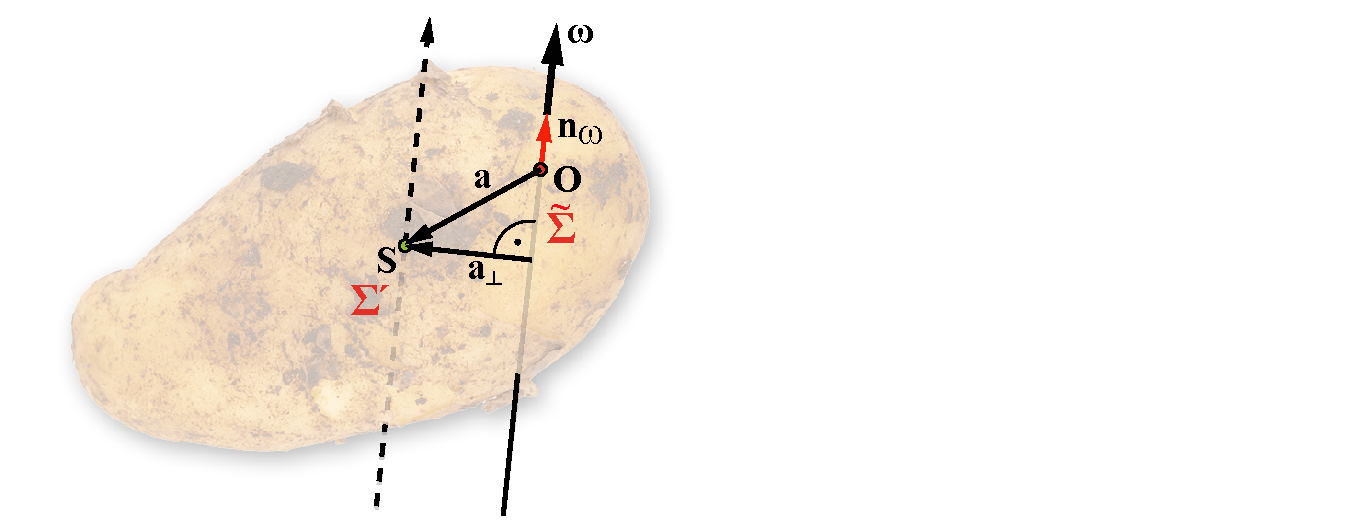
\includegraphics[width=\textwidth]{SteinerSatz.pdf}
  \caption[Steinerscher Satz.]{Steinerscher Satz. Die Rotation erfolge nun um eine Achse, die nicht durch den Schwerpunkt geht.
    Das neue Koordinatensystem $\tilde{\vec{\Sigma}}$ ist \emph{achsenparallel} zum k�rperfesten System (mit Ursprung im Schwerpunkt) $\vec{\Sigma}'$, allerdings mit seinem Ursprung nun auf der Drehachse.}
    \label{abb:bew_Steinerscher_Satz}
\end{figure}

Den Tr�gheitstensor hatten wir als Eigenschaft des K�rpers f�r die Berechnung
der kinetischen Energie \bzw des Drehimpulses eingef�hrt.
Wir wiederholen die Rechnung in dem neuen KOS $\tilde{\vec{\Sigma}}$ und k�nnen so erkennen, welchen Tr�gheitstensor wir f�r die neue Drehachse ben�tigen.%
\footnote{Wir erinnern daran, dass die kinetische Energie vom Bezugssystem abh�ngt
(\kap{bew_basics_of_systems}).}
Aus der kinetischen Energie \eqref{eq:bew_Kin_Energie_starrerK} wird jetzt
\begin{align}
  T  = T_\mathrm{trans} + T_\mathrm{rot}
  = T_\mathrm{trans} + \frac{1}{2} \int_V \tilde{\varrho}(\vec{\tilde{x}})\,
  (\vec{\omega} \times \vec{\tilde{x}})^2 \, \D^3 \tilde{x} ~ ,
\end{align}
wobei $T_\mathrm{trans}$ jetzt der Translation des Ursprungs von $\vec{\Sigma}'$
entspricht. 
F�hren wir die identische Rechnung zur Einf�hrung des Tr�gheitstensors ein zweites Mal aus, so sehen wir, dass sich der Tr�gheitstensor ergibt zu
\begin{align*}
  \tilde{\Theta}_{ij}
  &= \int_V \tilde{\varrho}(\vec{\tilde{x}}) \left (\vec{\tilde{x}}^2
    \delta_{ij} -\tilde{x}_i \tilde{x}_j \right ) \,\D^3 \tilde{x} \\
  &= \int_V \varrho(\vec{x}) \left ( (\vec{a} + \vec{x})^2 \delta_{ij} -
    (a_i+x_i) (a_j+x_j)  \right ) \,\D^3 x~.
\end{align*}
Ber�cksichtigt man erneut, dass Terme der Form $\varrho(\vec{x})x_i$
verschwinden, erh�lt man
\begin{align}
  \tilde{\Theta}_{ij}
  &= \int_v \varrho(\vec{x})\left ( \vec{x}^2 \delta_{ij} - x_i x_j \right )
  \,\D^3 x
  + \int_v \varrho(\vec{x}) \left ( \vec{a}^2 \delta_{ij} - a_i a_j \right )
  \,\D^3 x \notag \\
  &= \Theta_{ij} + M \left ( \vec{a}^2 \delta_{ij} - a_i a_j \right )\,.
\end{align}
Dies ist der \emph{Steinersche}%
\footnote{Jakob Steiner (1796--1863) war ein Schweizer Mathematiker,
der vor allem auf dem Gebiet der sogenannten synthetischen Geometrie arbeitete.}
Satz\index{Steinersche Satz}\indexp{Steiner, Jakob}:
Der Tr�gheitstensor (\bzw das Tr�gheitsmoment) f�r eine Rotation, die
nicht um den Schwerpunkt erfolgt, ist gleich der Summe aus dem Tr�gheitstensor
$\Theta$ f�r die Rotation um den Schwerpunkt und einem zweiten Anteil, der
so gro� ist, als w�rde die gesamte Masse des K�rpers im Schwerpunkt vereint um die neue Drehachse rotieren.\\
Daraus folgt insbesondere, dass das Tr�gheitsmoment f�r eine Rotation um den Schwerpunkt immer kleiner ist als das f�r jede dazu parallel verschobene Drehachse.
Diese Beziehungen gelten nat�rlich genauso f�r das Tr�gheitsmoment bez�glich einer festen Achse. Mit der Aufteilung
\begin{equation*}
  \omega^2 \left ( \vec{n_\omega} \times \vec{\tilde{x}} \right )^2 =
  \omega^2 \left ( \vec{n_\omega} \times \left ( \vec{a} + \vec{x} \right )
  \right )^2 =  \omega^2 \left ( {a_\perp}^2 + 2 \left (  \vec{n_\omega} \times
      \vec{a} \right ) \cdot \left (  \vec{n_\omega} \times \vec{x} \right )
    + {x_\perp}^2 \right )
\end{equation*}
in der kinetischen Energie erh�lt man (wobei lineare Terme in $\vec{x}$ im Integral wieder verschwinden)
\begin{align*}
  T_\mathrm{rot}
  &= \frac{1}{2} \omega^2 \int_V \varrho(\vec{x})\,{x_\perp}^2
    \,\D^3 x +  \frac{1}{2} \omega^2 \int_V \varrho(\vec{x})\, {a_\perp}^2 \,\D^3 x \\
  &= \frac{1}{2} \omega^2 \int_V \varrho(\vec{x}) \,{x_\perp}^2
    \,\D^3 x + \frac{1}{2} M \,{a_\perp}^2 \,\omega^2 
\end{align*}
oder das Tr�gheitsmoment
\begin{equation}
  \tilde{J} = J + M {a_\perp}^2 ~ , \label{eq:bew_SteinerSatz}
\end{equation}
also ebenfalls die Summe aus dem urspr�nglichen Tr�gheitsmoment und einem weiteren Term, der der Rotation der im Schwerpunkt vereinten Gesamtmasse senkrecht zur Drehachse entspricht.\\
Der Steinersche Satz erlaubt eine sehr simple Berechnung von Tr�gheitsmomenten f�r K�rper, die aus einfachen K�rperformen zusammengesetzt sind, da die Definition des Tr�gheitstensors \eqref{eq:bew_traegheitstensor} additiv ist (\probref{bew_traegheitsmomente}). 
Der Tr�gheitstensor eines starren K�rpers ist also die Summe der Tr�gheitstensoren seiner Teile (bei gleichem Bezugspunkt).
Dabei wird als Bezugspunkt f�r einen frei beweglichen starren K�rper am besten der Schwerpunkt gew�hlt, bei K�rpern, die in einem Punkt \bzw in einer Achse ortsfest sind, ist dieser Punkt \bzw diese Achse der Bezugspunkt/die Bezugsachse und das Tr�gheitsmoment wird �ber den Steinerschen Satz berechnet.

\subsection{Bewegungsgleichung des starren K�rpers}\label{kap:bew_BWG_StarrerK}

F�r die Bewegungsgleichungen eines starren K�rpers l�sst sich ausnutzen, dass wir bereits Ausdr�cke f�r den Gesamtimpuls und den Gesamtdrehimpuls gefunden haben.
Die Schwerpunktsbewegung wird durch die Summe der an den K�rper angreifenden Kr�fte bestimmt:
\begin{equation}
  \frac{\D \vec{P}_S}{\D t} =  \int_V \vec{f}(\vec{x})\, \D^3 x = \vec{F}\,.
\end{equation}
Die zeitliche �nderung des Gesamtdrehimpulses ergibt sich durch das
von au�en angreifende Drehmoment nach Gleichung
\eqref{eq:bew_Drehmoment_starrer_K}:
\begin{equation}
  \frac{\D\, \vec{L}}{\D t} = \vec{M}_\text{D}\,. \label{eq:bew_DrehimpulsSatz}
\end{equation}
Wir interessieren uns im Normalfall jedoch speziell f�r die Drehbewegung
des starren K�rpers unabh�ngig von der Bewegung des Schwerpunkts.
Gehen wir zus�tzlich noch davon aus, dass die Drehbewegung um den Schwerpunkt erfolgt \bzw die Drehachse durch den Schwerpunkt geht, beschreiben wir die Drehbewegung am besten im Schwerpunktsystem.
In diesem gilt $\vec{R}_S = \vec{0}$.
Damit verschwindet der Schwerpunktdrehimpuls $\vec{L}_S$ in Gleichung
\eqref{eq:bew_Gesamtdrehimpuls_starrer_K}.
Das Drehmoment aus
\eqref{eq:bew_Drehmoment_starrer_K} reduziert sich zu
\begin{equation*}
  \vec{M}_\text{D} = \int_V \left ( \vec{x} \times \vec{f}(\vec{x}) \right )\, \D^3 x
\end{equation*}
und man erh�lt
\begin{equation}
  \frac{\D\, \vec{L}_\mathrm{rot}}{\D t} = \frac{\D}{\D t} \underline{\vec{\Theta}} \,\vec{\omega}
  = \vec{M}_\text{D} = \int_V \left ( \vec{x} \times \vec{f}(\vec{x}) \right )\, \D^3 x
  ~ .
  \label{eq:bew_Drehbew_starrer_K}
\end{equation}
Die �nderung des Drehimpulses ist also gleich dem gesamten von au�en angreifenden Drehmoment.
Auch dieses Ergebnis hatten wir f�r starre Massepunktsysteme in \kap{bew_basics_of_systems} bereits hergeleitet.

\subsubsection{Euler-Gleichungen} \index{Euler-Gleichung}\label{kap:bew_Euler_Gl}

Die Bewegungsgleichung \eqref{eq:bew_Drehbew_starrer_K} f�r die Drehbewegung ist im raumfesten System mit zeitabh�ngigem Tr�gheitstensor $\Theta(t)$ gegeben. 
Vorteilhafter ist allerdings die Darstellung in einem k�rperfesten System, da dort $\underline{\vec{\Theta}}$ konstant ist.
Deswegen wollen wir nun die Bewegungsgleichung %mit der Drehmatrix $\mathbb{R}$
in ein k�rperfestes System $\vec{\Sigma}'$ transformieren.
Wir erhalten
\begin{subequations}
  \begin{align}
    \frac{\D}{\D t} \vec{L'}_\mathrm{rot} + \vec{\omega}' \times
    \vec{L}_\mathrm{rot}' = \vec{M}_\text{D}'
    \intertext{und da der Tr�gheitstensor im
    k�rperfesten System zeitlich konstant ist}
    \underline{\vec{\Theta}}' \dot{\vec{\omega}}' + \vec{\omega}' \times
    \underline{\vec{\Theta}}' \vec{\omega}'= \vec{M}_\text{D}' ~ .  \label{eq:bew_EulerGleichung01}
  \end{align}
\end{subequations}
Man beachte, dass selbst bei $\vec{M}_\text{D}'=\vec{0}$ der Drehimpuls nicht erhalten ist, da das System $\vec{\Sigma}'$ kein Inertialsystem ist.
Gleichung \eqref{eq:bew_EulerGleichung01} besagt, dass die zeitliche �nderung des Drehimpulses und das Drehmoment beim starren K�rper \ia nicht parallel sind.
Die Gleichungen sind nichtlinear in $\vec{\omega}'$ und deswegen relativ kompliziert zu l�sen.

Wir betrachten im Folgenden die Bewegung zun�chst nur in einem k�rperfesten System, welches als Haupttr�gheitsachsensystem gew�hlt ist. Dann k�nnen wir
die Komponentengleichungen von \eqref{eq:bew_EulerGleichung01} wie folgt schreiben:
\begin{equation}
  \begin{aligned}
    \Theta_{11} \, \dot{\omega}'_1 + (\Theta_{33}-\Theta_{22}) \,\omega'_2 \,\omega'_3 &= J_1 \, \dot{\omega}'_1 + (J_3-J_2) \,\omega'_2 \,\omega'_3 = M'_1\; ,\\
    \Theta_{22} \, \dot{\omega}'_2 + (\Theta_{11}-\Theta_{33}) \,\omega'_1 \,\omega'_3 &= J_2 \, \dot{\omega}'_1 + (J_1-J_3) \,\omega'_1 \,\omega'_3 = M'_2\; ,\\
    \Theta_{33} \, \dot{\omega}'_3 + (\Theta_{22}-\Theta_{11}) \,\omega'_1 \,\omega'_2 &= J_3 \, \dot{\omega}'_1 + (J_3-J_2) \,\omega'_1 \,\omega'_2 = M'_3 \;.
		\label{eq:bew_EulerGleichung02} 
  \end{aligned}
\end{equation}
Gleichungen \eqref{eq:bew_EulerGleichung01} und \eqref{eq:bew_EulerGleichung02} sind die \emph{Euler-Gleichungen} \index{Euler-Gleichung|textbf} f�r die Rotation eines starren K�rpers. 
Sie entsprechen den Newtonschen Bewegungsgleichungen f�r Massepunkte.
Der Einfachheit halber werden in der Literatur h�ufig die Striche f�r die Gr��en $\vec{M'}_\text{D}$ und $\vec{\omega}'$ des k�rperfesten Systems $\vec{\Sigma}'$ bei den Variablen weggelassen, wenn klar ist, dass man in $\vec{\Sigma}'$ rechnet.
Aber auch in diesen F�llen m�ssen wir uns immer in Erinnerung halten, dass die Gr��en in den Bewegungsgleichungen (Euler-Gleichungen) in Koordinaten des k�rperfesten Systems aufgeschrieben sind. 

\subsubsection{Euler-Winkel}\index{Euler-Winkel} \label{kap:bew_EulerWinkel}

Wir haben bei der Herleitung der Euler-Gleichungen angenommen, dass wir die momentane Winkelgeschwindigkeit in Koordinaten des k�rperfesten Systems $\vec{\Sigma}'$ ausdr�cken k�nnen. 
Das ergibt die einfache Struktur von \eqref{eq:bew_EulerGleichung02}, macht aber den Vektor $\vec{\omega}'$ sehr unanschaulich. 
Eleganter w�re eigentlich, die Bewegung im raumfesten System $\vec{\Sigma}$ zu beschreiben. 
Dazu f�hren wir drei zeitabh�ngige Winkel, die sogenannten \emph{Euler-Winkel} oder auch \emph{Eulerschen Winkel}\index{Euler-Winkel}\index{Eulersche Winkel} ein. 
Diese geben die momentane Orientierung des k�rperfesten Systems $\vec{\Sigma}'$ und damit des K�rpers im raumfesten System $\vec{\Sigma}$ an.

Wir nehmen an, dass $\vec{\Sigma}'$ und $\vec{\Sigma}$ einen gemeinsamen Ursprung haben. 
Durch eine zeitabh�ngige Rotation, welche eine Summe dreier Einzeldrehungen ist, kann man $\vec{\Sigma}$ in $\vec{\Sigma}'$ transformieren. 
Diese drei Winkel, die ben�tigt werden, um die Rotation vollst�ndig zu beschreiben, sind gerade die Euler-Winkel. 
Die Einzeldrehungen, f�r die das raumfeste System $\vec{\Sigma}$ (Achsen $\veceX$, $\veceY$, $\veceZ$) aus dem k�rperfesten $\vec{\Sigma}'$ (Achsen $\vecpeX$, $\vecpeY$, $\vecpeZ$) hervorgeht, sind:
\begin{enumerate}
\item Drehung um die Achse $\veceZ$ um den Winkel $\varphi$.
  (Die neue tempor�re $\veceX$-Achse hei�t Knotenlinie.)
\item Drehung um die Knotenlinie um den Winkel $\vartheta$.
\item Drehung um die nun erhaltene $\vecpeZ$-Achse um den Winkel $\psi$.
\end{enumerate}
Alle Drehungen erfolgen dabei in mathematisch positiver Richtung. Um letztlich die Bewegung des starren K�rpers im System $\vec{\Sigma}$ beschreiben zu k�nnen, m�ssen wir die Beziehung zwischen $\vec{\omega}$ und den Euler-Winkeln ermitteln.
Dazu betrachtet man eine kleine Drehung  $\vec{\omega}\,\D t$, die sich aus jeweils infinitesimalen �nderungen der Euler-Winkel um $\D \varphi$ um die Achse $\veceZ$, um $\D \vartheta$ um die Knotenlinie und um $\D \psi$ um die $\vecpeZ$-Achse zusammensetzt. 
Diese infinitesimale Drehung kann man aus geometrischen �berlegungen aus \figref{bew_EulerWinkel} ableiten und benutzt dabei die Rotationsmatrizen aus \kapitel{bew_rotating_systems}. 
Wir m�chten dies hier nicht im Einzelnen tun, sondern verweisen stattdessen auf \probref{bew_EulerWinkel} und geben hier lediglich das Ergebnis an:
\begin{align}
\vec{\omega}' = 
\begin{pmatrix}	\omega'_1 \\ \omega'_2 \\ \omega'_3 \end{pmatrix} = \,
\begin{pmatrix}
		\dot{\varphi}\,\sin\vartheta\,\sin\psi + \dot{\vartheta}\,\cos\psi \\
		\dot{\varphi}\,\sin\vartheta\,\cos\psi - \dot{\vartheta}\,\sin\psi \\
		\dot{\varphi}\,\cos\vartheta + \dot{\psi}
\end{pmatrix}. \label{eq:bew_EulerWinkel} 
\end{align}
\begin{figure}
  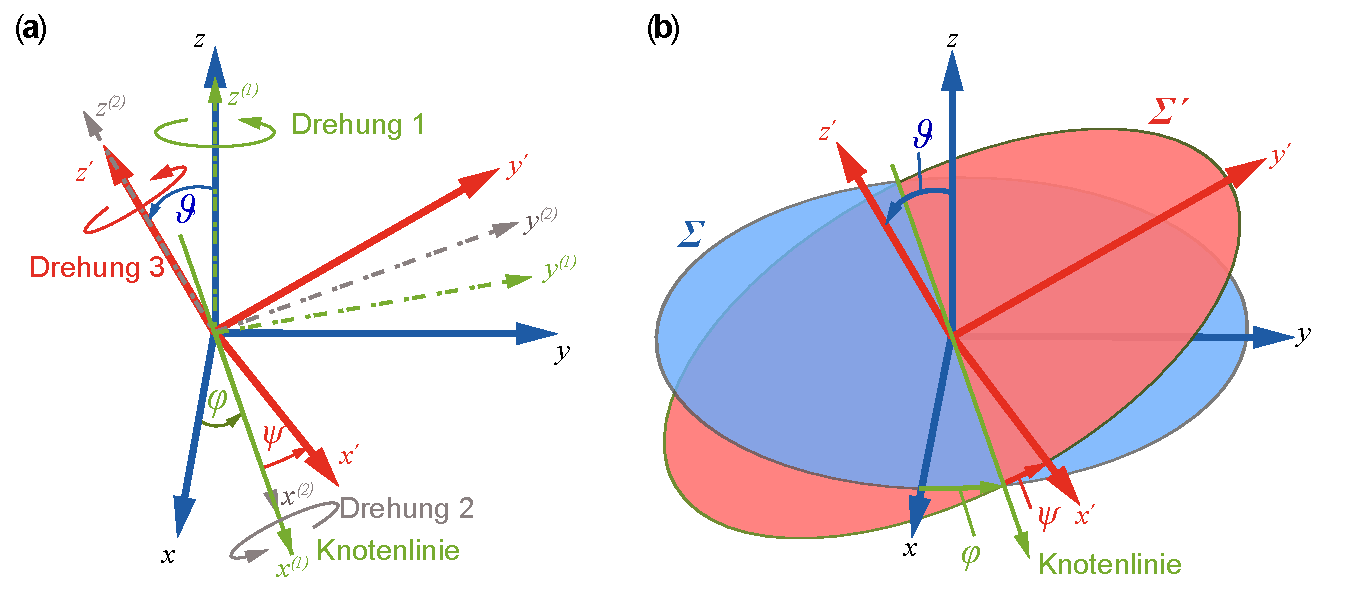
\includegraphics[width=0.95\textwidth]{EulerWinkel.pdf}
    \caption[Definition der Euler-Winkel.]{%
    \fa Definition der Euler-Winkel als Verkn�pfung dreier
    Rotationen. \fb
    Perspektivische Darstellung der Koordinatensysteme
    $\vec{\Sigma}$ und $\vec{\Sigma}'$ mit den Euler-Winkeln.}\label{abb:bew_EulerWinkel}
\end{figure}
Sind die Parameter f�r die Dynamik eines starren K�rpers durch $\vec{J}$ und $\vec{M}'$ gegeben, muss man also zun�chst aus den Euler-Gleichungen \eqref{eq:bew_EulerGleichung02} die momentane Winkelgeschwindigkeit $\vec{\omega}'(t)$ (in Koordinaten von $\vec{\Sigma}'$) bestimmen. 
Damit kann man dann die drei gekoppelten Diffentialgleichungen \eqref{eq:bew_EulerWinkel} nach $\varphi(t),\,\vartheta(t),\,\psi(t)$ l�sen. 
Das wird recht schwierig, denn einerseits ist \eqref{eq:bew_EulerGleichung02} eine nichtlineare DGL, andererseits liegen die gesuchten Gr��en (Euler-Winkel) in \eqref{eq:bew_EulerWinkel} auch noch als Argumente von Winkelfunktionen vor. Wir werden dennoch eine L�sung versuchen und uns dem allgemeinen Problem zun�chst �ber ein paar Spezialf�lle n�hern. Wir werden den Euler-Winkeln �brigens in der Himmelsmechanik (Band II, Kapitel 3) in etwas anderer Notation wieder begegnen.

\subsection{Kreisel} \label{kap:bew_Kreisel}

\subsubsection{Rotation eines \emph{kr�ftefreien} Kreisels} \index{Kreisel}\index{Kreisel!kr�ftefreier|textbf}\label{kap:bew_kfKreisel}

Ein Kreisel ist ein starrer K�rper, der um eine Achse rotiert.
In einer ersten Einschr�nkung werden wir davon ausgehen, 
dass er um eine Achse durch seinen Schwerpunkt rotiert.
Auf diesen k�nnen also die Eulerschen Kreiselgleichungen
\eqref{eq:bew_EulerGleichung02} angewendet werden.
Zun�chst werden wir den
Spezialfall des kr�ftefreien Kreisels betrachten.
F�r diesen verschwindet
also das Drehmoment $\MD$ und die Euler-Gleichungen
\eqref{eq:bew_EulerGleichung02} lassen sich auf die Form
\begin{equation}
  \begin{aligned}
    J_1 \, \dot{\omega}_1' + (J_3-J_2) \,\omega_2' \,\omega_3' = 0\\
    J_2 \, \dot{\omega}_2' + (J_1-J_3) \,\omega_1' \,\omega_3' = 0\\
    J_3 \, \dot{\omega}_3' + (J_2-J_1) \,\omega_1' \,\omega_2' = 0
  \end{aligned}
  \label{eq:bew_Kreisel_frei}
\end{equation}
bringen.
Man realisiert einen kr�ftefreien Kreisel \zb dadurch, dass man ihn im Schwerpunkt $S$ unterst�tzt und 
damit die Schwerkraft kompensiert.
Alternativ betrachtet man einen frei fallenden Kreisel im bewegten Koordinatensystem.
Sch�ne und instruktive Experimente zum kr�ftefreien Kreisel sind auf der ISS von Alexander 
Gerst\footnote{Alexander Gerst (geb.~1976) ist ein deutscher Geophysiker, Vulkanologe und Astronaut.
Er flog zweimal zur Internationalen Raumstation ISS\index{ISS!Internationale Raumstation}\indexp{Gerst, Alexander} 
und �bernahm am 3.\,10.\,2018 f�r fast drei Monate als erster Deutscher
die Funktion des ISS-Kommandanten.} 
durchgef�hrt worden \cite{Gerst2018}.

Man sieht an \eqref{eq:bew_Kreisel_frei} sofort, dass sich aus \eqref{eq:bew_Kreisel_frei} f�r den Fall einer Rotation um eine der Haupttr�gheitsachsen 
(also um eine der Koordinatenachsen von $\vec{\Sigma}'$, \zb $\omega_1'=\omega_0'$ mit $\omega_2'=\omega_3'=0$) 
$\dot{\vec{\omega}'}=\vec{0}$
ergibt und die Rotation somit zeitlich konstant ist. 

Dies gilt jedoch nur f�r eine exakte Ausrichtung entlang einer der
Haupttr�gheitsachsen, was sich in der Realit�t nicht erf�llen lassen wird.
Um die Stabilit�t solcher Drehungen nahe einer der Haupttr�gheitsachsen zu untersuchen, 
legen wir das Koordinatensystem so, dass $J_1 > J_2 > J_3$ gilt. 
Weiterhin nehmen wir an, dass wir eine kleine St�rung $\vec{\Delta\omega}'$ der Rotation um eine der Haupttr�gheitsachsen haben.
Setzt man \zb f�r eine Rotation um die $\vecpeX$-Achse einen \anf{gest�rten} Vektor der Winkelgeschwindigkeit 
\begin{equation}
  \vec{\omega}_0' + \vec{\Delta\omega}' = 
  \begin{pmatrix} \omega_0'
    + \Delta\omega_1'(t) \\  \Delta\omega_2'(t) \\ \Delta\omega_3'(t)
  \end{pmatrix} \label{eq:bew_Kreisel_frei_lin}
\end{equation}
an und linearisiert die Bewegungsgleichungen in den $\Delta\omega_i'$, so
findet man als Ergebnis, dass die St�rung in der
$\vecpeY$-$\vecpeZ$-Ebene erhalten bleibt, jedoch nicht gr��er wird.
Eine
Rotation um die $\vecpeX$-Achse ist also stabil.
Gleiches findet man f�r
eine Rotation um die $\vecpeZ$-Achse.
Jedoch wird, falls eine Rotation
um die $\vecpeY$-Achse gest�rt wird, die St�rung exponentiell anwachsen.
Eine solche Rotation ist also instabil.
Die ausf�hrliche Betrachtung erfolgt
numerisch in  Beispiel \ref{bsp:bew_unsymm_Kreisel} und \probref{bew_freier_Kreisel}. 
Wir merken uns jedoch, dass f�r einen nicht-symmetrischen
Kreisel die Rotationen nur um die beiden Haupttr�gheitsachsen mit dem jeweils gr��ten bzw. kleinsten
Tr�gheitsmoment stabil sind.
Eine Rotation um die Haupttr�gheitsachse mit dem
mittleren Tr�gheitsmoment ist instabil.

%BEISPIEL %%%%%%%%%%%%%%%%%%%%%%%%%%%%%%%%%%%%%%%%%%%%%%%%%%%%%%%%%%%%%%%%%%%%%%%%%%%%%%%%%%
\begin{example}{St�rung der Rotation um freie Haupttr�gheitsachsen }
\label{bsp:bew_unsymm_Kreisel}
\medskip

Die Bewegungsgleichungen \eqref{eq:bew_Kreisel_frei} des kr�ftefreien unsymmetrischen
Kreisels lassen sich numerisch einfach integrieren.
Damit l�sst sich die
Stabilit�t der Rotationen um die Haupttr�gheitsachsen gut analysieren.
Wir
w�hlen das Verh�ltnis der drei Haupttr�gheitsmomente $J_1 : J_2 : J_3 =
3:4:5$, $J_1$ und $J_2$ sind also die extremen Tr�gheitsmomente und $J_2$
liegt dazwischen.
Die N�herung f�r kleine St�rungen (siehe \probref{bew_freier_Kreisel}) sagt voraus, dass die
Rotationen um die $\vecpeX$- und $\vecpeZ$-Achsen stabil, die um
$\vecpeY$ instabil sein sollten.
Die exemplarischen Ergebnisse sind (numerisch im \mscr{} 
\mlbewref{KfKreiselFreieAchsen.m} ausgef�hrt) wie folgt:

\begin{itemize}
\item F�r eine Rotation um die $\vecpeX$-Achse mit
  $\omega_1' = 1/\mathrm{s}$, die leicht durch einen zus�tzlichen Beitrag
	$\Delta \omega_2'$ gest�rt wird, ergibt sich Bild \figref{bew_KfKreiselstabil}.
 
\begin{center}
    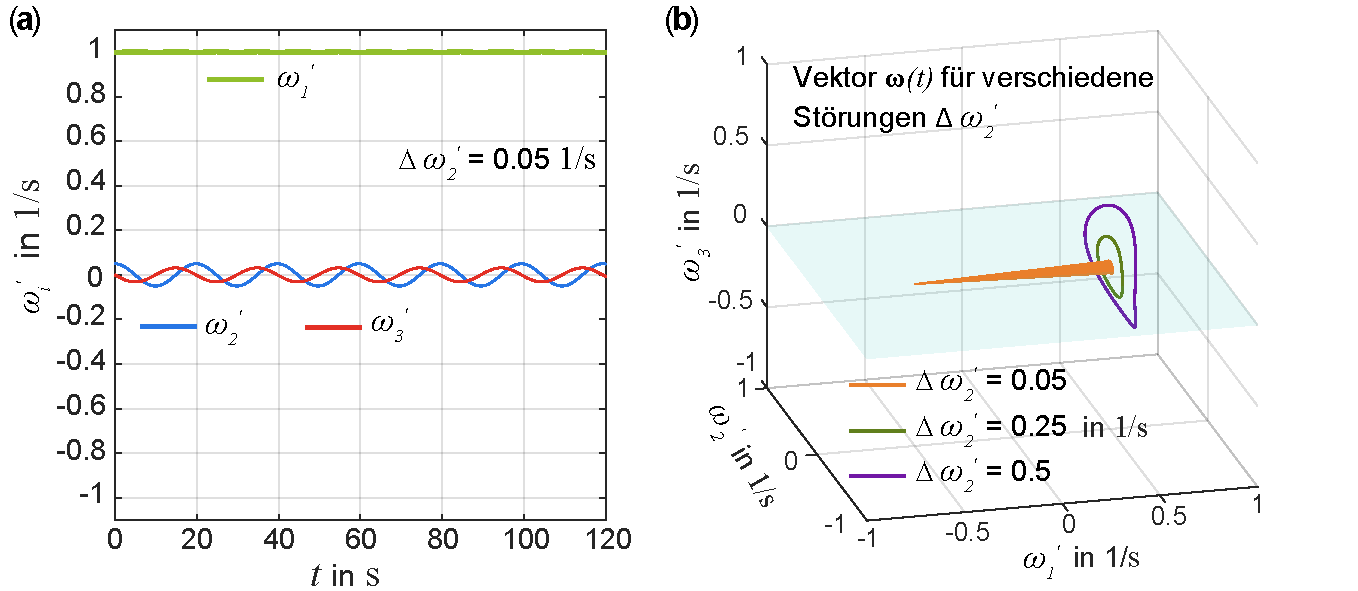
\includegraphics[width=\textwidth]{KfKreiselstabil.pdf}
\captionof{figure}{Stabile Rotation eines kr�ftefreien Kreisels um seine Hauptachsen.}\label {abb:bew_KfKreiselstabil}
\end{center}

Im linken Teil von \figref{bew_KfKreiselstabil} sieht man den zeitlichen
Verlauf der drei Kreisfrequenzen f�r eine Anfangsst�rung von
$\Delta \omega_2'= \SI{0.05}{\per\s}$.
Die Erwartung aus der linearen N�herung der St�rung \eqref{eq:bew_Kreisel_frei_lin}
ist gut erf�llt. Es ergibt sich eine Oszillation der St�rung zwischen der
$\vecpeY$- und $\vecpeZ$-Richtung, sie wird jedoch betragsm��ig nicht gr��er.
Die Rotation um die $\vecpeX$-Achse �ndert sich kaum. Dies erkennt man auch
in der rechten Abbildung, in der der zeitliche Verlauf aller drei Komponenten
von $\vec{\omega}'$ dargestellt ist.
F�r die kleinen Anfangsst�rungen $\Delta \omega_2' = \SI{0.05}{\per\s}$ und
$\Delta\omega_3' = \SI{0.05}{\per\s}$ oszilliert die Spitze des Vektors
$\vec{\omega}'$ mit kleinen Abst�nden um den eigentlich beabsichtigten Wert
$\vec{\omega}' = (1.0,0,0)\SI{}{\per\s}$ (linkes Bild).
Erst f�r die deutlich gr��ere St�rung von $\Delta \omega_2' \geq \SI{0.25}
{\per\s}$ ergibt sich eine leichte sichtbare Abweichung der Richtung des
Vektors $\vec{\omega}'$ und auch eine zeitliche Variation von $\omega_1'(t)$.

\item Nun betrachten wir eine Rotation um die $\vecpeY$-Achse (mit dem mittleren Tr�gheitsmoment $J_2$ 
und der Winkelgeschwindigkeit $\omega_2' = \SI{1.0}{\per\s}$), die 
wiederum durch einen kleinen zus�tzlichen Beitrag, hier nun $\Delta \omega_1'$, gest�rt wird.
Die Erwartung aus der linearen N�herung mit dem Ansatz
\eqref{eq:bew_Kreisel_frei_lin} ist nun, dass sich die St�rung exponentiell
vergr��ert.  Dies geschieht auch f�r die Anfangsst�rung
$\Delta \omega_1' = \SI{0.05}{\per\s}$ zun�chst.
Dann wird die St�rung jedoch so
gro�, dass die lineare N�herung nicht mehr g�ltig ist.
Es ergibt sich eine in (\figref{bew_KfKreiselinstabil}) deutlich sichtbare
erhebliche Abweichung von der urspr�nglichen Rotation, bei der im Zeitverlauf
alle drei Komponenten von $\vec{\omega}'$ �hnlich gro�e Werte annehmen und die
Bewegung nichts mehr mit einer reinen Rotation um die $\vecpeY$-Achse
zu tun hat.
Obwohl die St�rung am Beginn nicht gr��er ist als im vorherigen
Beispiel, ergibt sich nach kurzer Zeit ein vollst�ndig anderes Verhalten.
Durch die Instabilit�t der Achse spielt es fast keine Rolle, wie gro�
die Anfangsst�rungen sind, wie man im rechten Teil von
\figref{bew_KfKreiselinstabil} erkennt. F�r die Anfangsst�rungen
$\Delta \omega_1' = \SI{0.05}{\per\s}$, $\SI{0.25}{\per\s}$ und
$\SI{0.5}{\per\s}$ ergibt sich jeweils ein sehr �hnliches Verhalten. 

\begin{center}
    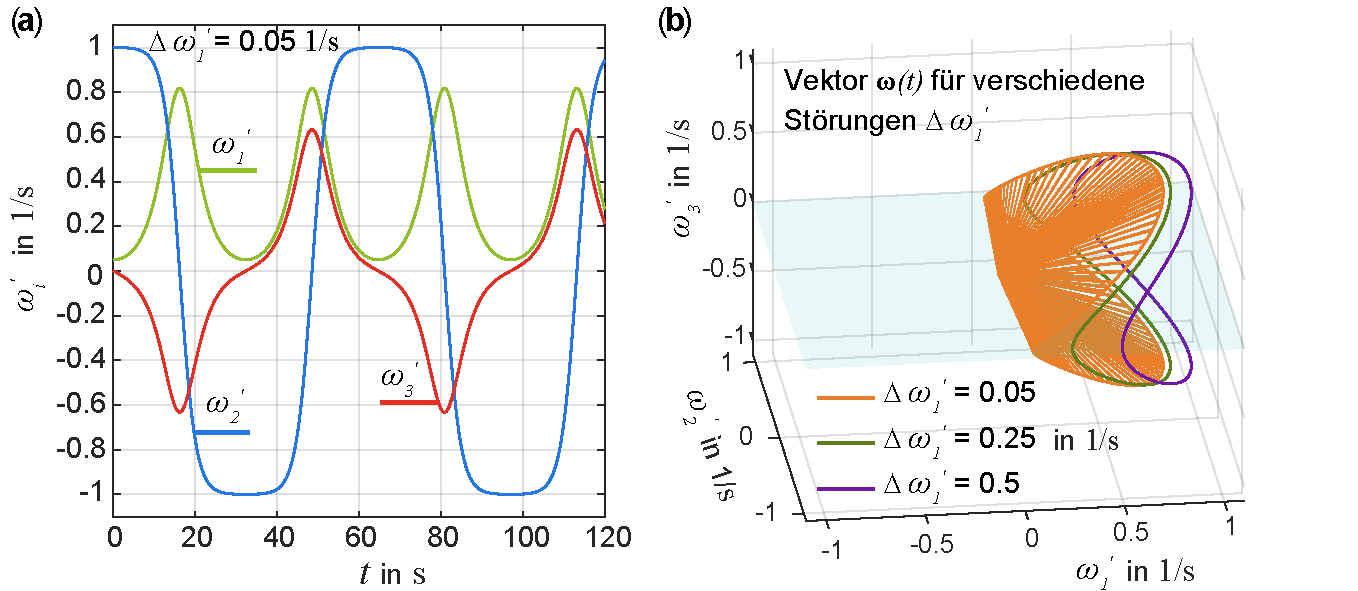
\includegraphics[width=\textwidth]{KfKreiselinstabil.pdf}
\captionof{figure}{Instabile Rotation eines kr�ftefreien Kreisels um seine freien Hauptachsen.}\label {abb:bew_KfKreiselinstabil}
\end{center}

\end{itemize}
\end{example}
%BEISPIEL %%%%%%%%%%%%%%%%%%%%%%%%%%%%%%%%%%%%%%%%%%%%%%%%%%%%%%%%%%%%%%%%%%%%%%%%%%%%%%%%%%

\subsubsection{Rotation eines kr�ftefreien \emph{symmetrischen} Kreisels} \index{Kreisel!kr�ftefreier!}\index{Kreisel!symmetrischer}\label{kap:bew_Kreisel_kraeftefrei}

Bisher haben wir nur freie Rotationen um die Haupttr�gheitsachsen des Kreisels betrachtet.
Wir wollen jetzt die Bewegung des Kreisels einschr�nken und den Kreisel \emph{im Schwerpunkt} festhalten \bzw unterst�tzen. Dieser Kreisel ist dann auch kr�ftefrei.
Eine solche Kr�ftefreiheit kann man dadurch realisieren, dass man den Kreisel in einer sogenannten kardanischen\footnote{Gerolamo Cardano\indexp{Cardano, Gerolamo} (1501--1576) war ein italienischer Arzt, Philosoph und Mathematiker. Er arbeitete auf vielen Gebieten, \ua in der Wahrscheinlichkeitsrechnung und Kombinatorik, in der Erforschung von Krankheiten wie Tuberkulose und Typhus und an mechanischen Konstruktionen. Nach ihm ist die kardanische Aufh�ngung und die Kardanwelle benannt.} (oder cardanischen)\index{Kardanische Aufh�ngung}\index{Cardanische Aufh�ngung} Aufh�ngung befestigt (Abb. \figref{bew_KfSymmKrRealisierung}). Alternativ kann man sich nat�rlich auch f�r entsprechende Studien an kr�ftefreien Kreiseln auf einen Raumflug begeben.\\
Als weiteren Spezialfall wollen wir den kr�ftefreien Kreisel als symmetrisch annehmen. 
Darunter versteht man
einen Kreisel, f�r den zwei Tr�gheitsmomente identisch sind, $J_1 = J_2
= J_{12} \neq J_3$. Die Achse $\vecpeZ$, die senkrecht zur den beiden
identischen Haupttr�gheitsmomenten steht, hei�t Figurenachse $\vec{f}$. 

\begin{figure}
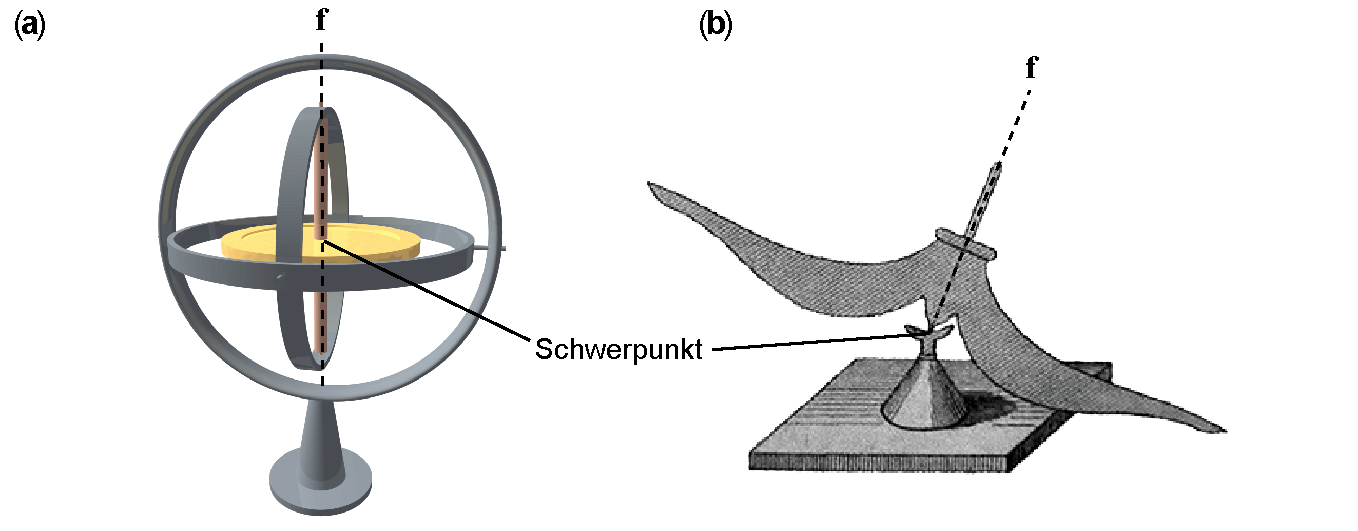
\includegraphics[width=\textwidth]{KfSymmKrRealisierung.pdf} 
	\caption[Realisierung des kr�ftefreien symmetrischen Kreisels.]{Realisierung des kr�ftefreien symmetrischen Kreisels \fa Kardanische Aufh�ngung (Euler-Kreisel) und \fb Unterst�tzung im Schwerpunkt (nach Klein\footnotemark\indexp{Klein, Felix Christian} und Sommerfeld \cite{Klein1910}).} \label{abb:bew_KfSymmKrRealisierung}
\end{figure}
\footnotetext{Felix Christian Klein (1849--1925) war ein deutscher Mathematiker, der im 19.~Jahrhundert bedeutende Fortschritte vor allem in der Geometrie erzielte. Klein besch�ftigte sich mit der Funktionentheorie und k�mmerte sich um die Anwendung der Mathematik. Er engagierte sich sehr f�r die Mathematikdidaktik und die Lehre generell. Sommerfeld war einer seiner besten Sch�ler.}

Da wir in diesem Kapitel den Kreisel sowohl im System $\vec{\Sigma}$ als auch im mitbewegten System $\vec{\Sigma'}$ betrachten wollen, kennzeichnen wir wie vereinbart die Gr��en im mitrotierenden System mit Strichen.
Aus den Kreiselgleichungen \eqref{eq:bew_EulerGleichung02} folgt damit
\begin{equation*}
  J_3\,\dot{\omega}_3' = 0 \qquad \text{und} \qquad \omega_3' = \con~ .
\end{equation*}
Setzt man mit dem Wissen, dass $\omega_3'$ konstant ist,
\begin{equation*}
  \Omega = \frac{J_3-J_{12}}{J_{12}} \,\omega_3' = \con~ ,
\end{equation*}
erh�lt man f�r die Bewegungsgleichungen der anderen beiden Komponenten
die gekoppelten Differentialgleichungen
\begin{equation*}
  \begin{aligned}
    \dot{\omega}_1' &= - \Omega \, \omega_2' ~ ,\\
    \dot{\omega}_2' &= \phantom{-}  \Omega \, \omega_1' ~ .\\
  \end{aligned}
\end{equation*}
Die L�sungen lassen sich einfach finden, da dieses DGL-System in eine DGL zweiter Ordnung �berf�hrt werden kann, 
die der harmonischen Schwingungsgleichung entspricht. Insgesamt erh�lt man
\begin{equation}
  \vec{\omega}' = 
	\begin{pmatrix} \omega_1' \\ \omega_2' \\ \omega_3' \end{pmatrix} = 
	\begin{pmatrix} \omega_\perp' \, \cos(\Omega \,t + \Delta
    \alpha) \\ \omega_\perp' \, \sin(\Omega\, t + \Delta \alpha) \\
    \omega_3' \end{pmatrix}
  \label{eq:bew_Nutation_omega}
\end{equation}
mit der zeitunabh�ngigen (konstanten) Amplitude
$\omega_\perp' = \sqrt{{\omega_1 '}^2 + {\omega_2 '^2}}$ der Drehung mit der betragsm��ig 
konstanten Winkelgeschwindigkeit
$\omega' = \left| \vec{\omega}'\right| = \sqrt{{\omega_\perp'}^2 + {\omega_3'}^2}$
um die $\vecpeZ$-Achse.
F�r den Drehimpuls gilt
\begin{equation}
  \vec{L}' = 
	\begin{pmatrix} J_{12}\,\omega_1' \\ J_{12}\,\omega_2' \\ J_3\, \omega_3' \end{pmatrix} =
	\begin{pmatrix} J_{12} \, \omega_\perp' \, \cos(\Omega\, t + \Delta
    \alpha) \\ J_{12} \, \omega_\perp' \, \sin(\Omega\, t + \Delta \alpha) \\
    J_3 \, \omega_3' \end{pmatrix} ~
  \label{eq:bew_Nutation_L}
\end{equation}

und damit $L'^2 = \con$, wie zu erwarten war.
Man sieht aus \eqref{eq:bew_Nutation_omega} und \eqref{eq:bew_Nutation_L}
also, dass sowohl $\vec{\omega}'$ als auch $\vec{L}'$ eine Drehung um
die $\vecpeZ$-Achse (die Figurenachse) des k�rperfesten Systems ausf�hren, allerdings in
unterschiedlicher Art und Weise, da nach \eqref{eq:bew_Nutation_L} $\vec{L}'$ und $\vec{\omega}'$ unterschiedliche
Richtungen haben (siehe \figref{bew_KfSymmKrNutation} a). Man nennt diese Bewegung \emph{Nutation} (aus dem Lateinischen \textit{nutare} f�r "`nicken"').\index{Nutation|textbf}\footnote{Vielfach wird diese Bewegung auch \textit{(regul�re) Pr�zession}\index{Pr�zession|textbf}\index{Pr�zession!regul�re|textbf} genannt, vor allem im angels�chsischen Raum. Auch Klein und Sommerfeld \cite{Klein1910} verwendeten diesen Begriff. Da wir den Begriff Pr�zession f�r eine Bewegung beim schweren Kreisel reservieren wollen, verwenden wir hier den Begriff Nutation.}

\begin{figure}
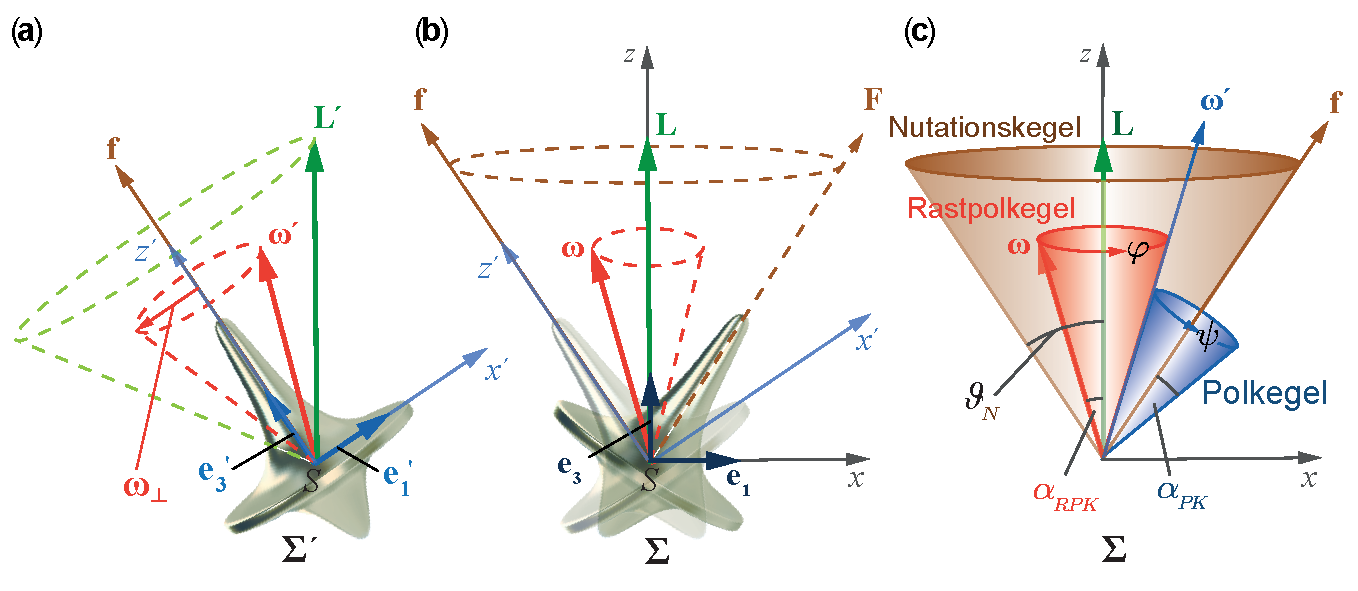
\includegraphics[width=\textwidth]{KfSymmKrNutation.pdf} 
	\caption[Nutation eines kr�ftefreien symmetrischen Kreisels.]{Ein kr�ftefreier symmetrischer Kreisel f�hrt eine Nutationsbewegung aus.
    \fa Im k�rperfesten System f�hren die Drehachse $\vec{\omega}'$ und auch der Drehimpuls $\vec{L}'$ eine Kreisbewegung um die Figurenachse $\vec{F}=\vecpeZ$
    aus. \fb Im raumfesten System ist der Drehimpuls f�r die kr�ftefreie Bewegung konstant. Man sieht eine Drehbewegung der Figurenachse und
    der momentanen Drehachse um die feststehende Drehimpulsachse. \fc �bersicht der Rotationsbewegungen der einzelnen Achsen des kr�ftefreien symmetrischen
Kreisels.
$\vartheta_\text{N}, \alpha_\text{PK}, \alpha_\text{RK}$ sind die �ffnungswinkel von Nutations-, Pol- \bzw Rastpolkegel.}\label{abb:bew_KfSymmKrNutation}
\end{figure}
Die Nutation ist zwar dynamisch, aber in ihrer periodischen Entwicklung stabil.
Wir nehmen diese jedoch f�r gew�hnlich nicht im k�rperfesten System wahr,
sondern beobachten sie aus dem raumfesten System heraus.
Da die Bewegung nach Voraussetzung kr�ftefrei ist und somit auch kein Drehmoment wirkt,
ist in diesem System der Drehimpuls nach Richtung und Betrag konstant,
die Drehimpulsachse liegt folglich stabil im Raum.
Die Figurenachse $\vec{f} = \vecpeZ$ rotiert auf dem \emph{Nutationskegel} mit dem 
�ffnungswinkel $\vartheta_\text{N}$ um die Drehimpulsachse. 
Wir wollen die Nutation im raumfesten System im folgenden Beispiel n�her untersuchen.
\newpage
%Begin BEISPIEL %%%%%%%%%%%%%%%%%%%%%%%%%%%%%%%%%%%%%%%%%%%%%%%%%%%%%%%%%%%%%%%%%%%%%%%%%%%%%%%%%%
\begin{example}{Dynamik der Nutation eines kr�ftefreien symmetrischen Kreisels}
  \medskip
	
	Es wurde bereits erw�hnt, dass die Nutationsbewegung dadurch gekennzeichnet ist, 
	dass die Drehimpulsachse fest im Raum steht,
  da aufgrund der Kr�fte- und Drehmomentfreiheit der Drehimpuls erhalten ist.
  Die Beschreibung der Drehbewegung im raumfesten System erfolgt mithilfe der Euler-Winkel
  \eqref{eq:bew_EulerWinkel}.
  Man erh�lt mit
  \eqref{eq:bew_Nutation_omega}
  \begin{equation}
    \begin{pmatrix} \omega_1'\\ \omega_2' \\ \omega_3' \end{pmatrix}
    = \begin{pmatrix} \omega_\perp' \, \cos(\Omega \,t + \Delta
      \alpha) \\ \omega_\perp' \, \sin(\Omega\,t + \Delta \alpha) \\
      \omega_3' \end{pmatrix}
    = \begin{pmatrix}
      \dot{\varphi}\,\sin\vartheta\,\sin\psi + \dot{\vartheta}\,\cos\psi \\
      \dot{\varphi}\,\sin\vartheta\,\cos\psi - \dot{\vartheta}\,\sin\psi \\
      \dot{\varphi}\,\cos\vartheta + \dot{\psi}
    \end{pmatrix} \; .
    \label{eq:bew_DGL_Eulerwinkel_Nutation}
  \end{equation}
  Das raumfeste System legen wir so, dass die Drehimpulsachse mit der
  $\veceZ$-Achse des KOS �bereinstimmt.
  Dann wird die Neigung der Figurenachse
  gegen�ber dem Drehimpuls gerade durch den Euler-Winkel $\vartheta$ ausgedr�ckt.
  Dieser berechnet sich nach nach \eqref{eq:bew_Nutation_L} zu
  \begin{equation}
    \vartheta_\text{N} = \arctan \lk \frac{\sqrt{{L_x'}^2 + {L_y'}^2}}{L_z'} \rk = \arctan \left ( \frac{J_{12} \omega_\perp'}{J_3 \omega_3'}
    \right ) \; . \label{eq:bew_Nutationswinkel}
  \end{equation}
  und ist, wie bereits erw�hnt, konstant.
  Gleichung \eqref{eq:bew_DGL_Eulerwinkel_Nutation} vereinfacht sich zu
  \begin{equation}
	   \begin{pmatrix} \omega_1'\\ \omega_2' \\ \omega_3' \end{pmatrix} =
		 \begin{pmatrix} \omega_\perp' \, \cos(\Omega\,t + \Delta
      \alpha) \\ \omega_\perp' \, \sin(\Omega\,t + \Delta \alpha) \\
      \omega_3' \end{pmatrix}
    = \begin{pmatrix}
      \dot{\varphi}\,\sin\vartheta_\text{N}\,\sin\psi \\
      \dot{\varphi}\,\sin\vartheta_\text{N}\,\cos\psi \\
      \dot{\varphi}\,\cos\vartheta_\text{N} + \dot{\psi}
    \end{pmatrix} \; .
    \label{eq:bew_DGLEuler_Nutation2}
  \end{equation}
  Eine L�sung findet man leicht, indem man die ersten beiden Zeilen dieser
  vektoriellen Gleichung quadriert und addiert.
  Daraus ergibt sich sofort
  \begin{equation}
    \dot{\varphi} = \frac{\omega_\perp'}{\sin\vartheta_\text{N}} = \Omega' \qquad
    \text{bzw.}\qquad \varphi(t) = \frac{\omega_\perp'}{\sin\vartheta_\text{N}}\,t  +\varphi_0 = \Omega' \,t +\varphi_0 \,. \label{eq:bew_DGLEuler_Nutation2a}
  \end{equation}
  Die dritten Zeile f�hrt mit diesem Resultat auf
  \begin{align*}
    \dot{\psi} &= \omega_3' - \omega_\perp' \cot\vartheta_\text{N} = \omega_3'
    - \frac{J_3\,\omega_3'}{J_{12}} = \frac{J_{12}-J_3}{J_{12}}\,\omega_3'
                 = \con = -\, \Omega \\
    \text{\bzw} \qquad \psi(t) &= -\, \Omega \, t + \psi_0 \; .
  \end{align*}
  Ein Vergleich mit den ersten beiden Zeilen legt die Integrationskonstante
  $\psi_0$ fest auf $\psi_0 = -\Delta \alpha \pm \pi/2$, sodass
  \begin{equation}
    \psi(t) = -\,\Omega\, t  - \Delta \alpha \pm \frac{\pi}{2} \; . \label{eq:bew_DGLEuler_Nutation2b}
  \end{equation}
  Damit haben wir in diesem geeignet gew�hlten Koordinatensystem $\vec{\Sigma}$ alle drei Euler-Winkel bestimmt.
  Die Figurenachse, die mit dem konstanten 
  Winkel $\vartheta_\text{N}$ gegen den konstanten Drehimpuls geneigt ist, l�uft mit der konstanten Winkelgeschwindigkeit $\dot{\varphi} = \Omega'$ um den raumfesten Drehimpuls herum.
	Dazu dreht sich der Kreisel mit der ebenfalls konstanten Winkelgeschwindigkeit $\dot{\psi} = \Omega$ um seine Figurenachse. 
	Dieses Ergebnis l�sst sich auch numerisch finden.
  Dazu bringt man die Gleichungen \eqref{eq:bew_DGLEuler_Nutation2} auf eine geeignete
  Form, in der die drei Zeitableitungen der Euler-Winkel isoliert auf den linken Seite des Gleichungssystems stehen.
	Dies gelingt \zb f�r $\dot{\varphi}$ durch
  die Multiplikation der ersten Zeile mit $\sin\psi$ und Addition der mit
  $\cos\psi$ multiplizierten zweiten Zeile.  Analog ergibt sich durch Multiplikation der ersten Zeile mit $\cos\psi$
  und Subtraktion der zweiten mit $\sin\psi$ multiplizierten Zeile eine
  Differentialgleichung f�r $\dot{\vartheta}$ und schlie�lich gewinnt man aus der dritten Zeile von \eqref{eq:bew_DGLEuler_Nutation2} 
	unter Nutzung der Beziehung f�r $\dot{\varphi}$ eine Beziehung f�r $\dot{\psi}$. Insgesamt erh�lt man also
\begin{align}
  \frac{\D}{\D t}\, {\begin{pmatrix}\varphi\\\vartheta\\\psi\end{pmatrix}}
    =
    \begin{pmatrix}
      \frac{\sin\psi}{\sin\vartheta} & \frac{\cos\psi}{\sin\vartheta} & 0 \\
      \cos\psi               & -\sin\psi              & 0 \\
      -\sin\psi\cot\vartheta         & -\cos\psi\cot\vartheta         & 1
    \end{pmatrix} \,
    \vec{\omega}\,.
  \label{eq:bew_DGLEuler_Nutation2c}
\end{align}
Integriert man diese gekoppelten Differentialgleichungen erster Ordnung mit den passenden Anfangsbedingungen $\vartheta(0) = \vartheta_\text{N}$,
$\psi(0) = -\Delta \alpha \pm \frac{\pi}{2}$ (und einem beliebigen $\varphi(0)$), so findet man die in \figref{bew_SymmKreiselEulerWinkel} 
dargestellte numerische L�sung f�r die Winkelgeschwindigkeit $\vec{\omega}$ und die Euler-Winkel (\mscr{} \mlbewref{KfSymmKreiselNutation.m}).
Man findet hier also, sofern man das raumfeste Koordinatensystem durch  die oben gegebenen Anfangsbedingungen so legt, dass der Drehimpuls auf
die $\veceZ$-Achse f�llt, f�r die Euler-Winkel sowohl das konstante  $\vartheta = \vartheta_\text{N}$ als auch die konstanten Winkelgeschwindigkeiten 
von $\dot{\varphi}$ und $\dot{\psi}$ wieder.
Im \mscr{} \mlbewref{KfSymmKreiselSimulation.m} ist eine Simulationsrechnung der 
Nutation des kr�ftefreien symmetrischen Kreisels sowohl im k�rper- als auch im raumfesten System ausgef�hrt.
\begin{center}
    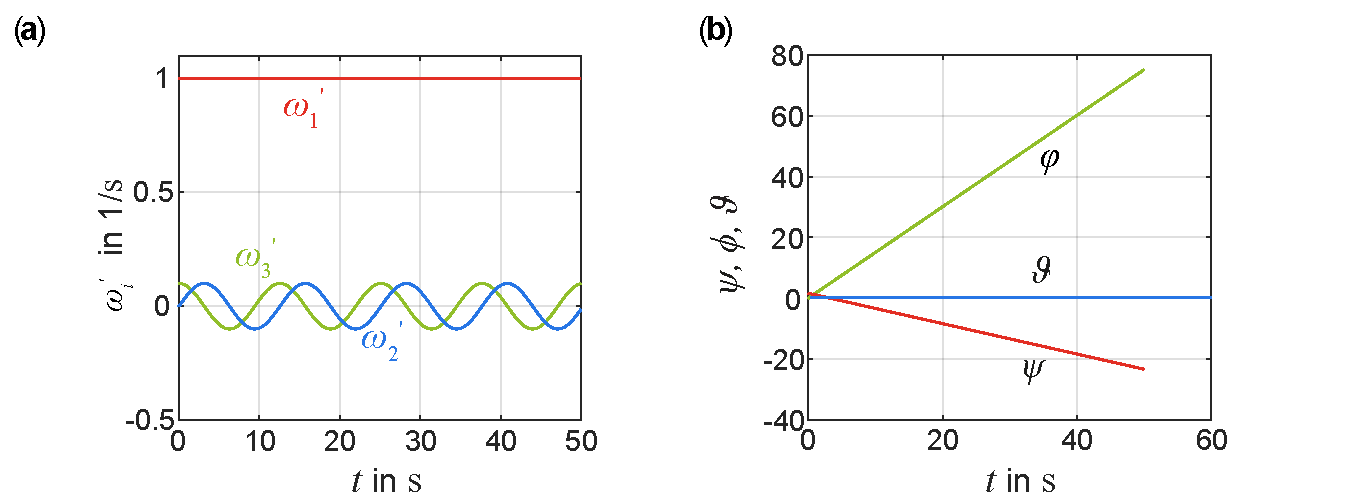
\includegraphics[width=\textwidth]{SymmKreiselEulerWinkel.pdf}
\captionof{figure}[Dynamik der Nutation eines kr�ftefreien symmetrischen Kreisels.]{Dynamik der Nutation eines kr�ftefreien symmetrischen Kreisels. \fa Zeitliche Entwicklung von $\vec{\omega}$, \fb Zeitliche Entwicklung der Euler-Winkel. Parameter: $J_1 = J_2 = \SI{1}{\kg\metre\squared}\,,\, J_3 = \SI{1.5}{\kg\metre\squared}$.} \label{abb:bew_SymmKreiselEulerWinkel}
\end{center}
\end{example}
%Ende BEISPIEL %%%%%%%%%%%%%%%%%%%%%%%%%%%%%%%%%%%%%%%%%%%%%%%%%%%%%%%%%%%%%%%%%%%%%%%%%%%%%%%%%%
Wie wir gesehen haben, gibt es im raumfesten System $\vec{\Sigma}$ neben der Nutation der Figurenachse um die Drehimpulsachse auch 
eine Drehung der Achse der Winkelgeschwindigkeit $\vec{\omega}$ um die $\vec{L}$-Achse. Diese rotiert auf dem sogenannten \emph{Rastpolkegel}, der den 
�ffnungswinkel 
\begin{align}
	\alpha_\text{RPK} = \arctan{\frac{\omega_\perp'}{\omega_3'}} = \arctan{\frac{\sqrt{{\omega_1'}^2+{\omega_2'}^2}}{\omega_3'}} \label{eq:bew_Nutation_alphaRPK}
\end{align}
hat. Im k�rperfesten System $\vec{\Sigma}'$ hingegen rotiert diese $\vec{\omega}$-Achse um die Figurenachse auf dem \emph{Polkegel}, dessen �ffnungswinkel $\alpha_\text{PK}$ durch den Winkel zwischen den Komponenten $L_3 \,\vecpeZ$ und $\vec{\omega}_3'\,\vecpeZ$ gegeben ist: 
\begin{align}
	\alpha_\text{PK} = \arctan{\frac{\Omega\,\sin\vartheta_\text{N}}{\Omega' + \Omega\,\cos\vartheta_\text{N}}}\,. \label{eq:bew_Nutation_alphaPK}
\end{align}
Anschaulich kann man sich das so vorstellen, dass der Polkegel auf dem Rastpolkegel abrollt, wobei die
Kontaktlinie beider Kegel gerade der Achse der Winkelgeschwindigkeit entspricht (die dort quasi \anf{rastet}, daher der Name Rastpolkegel).
Diese komplizierten Bewegungen der einzelnen Achsen sind in \figref{bew_KfSymmKrNutation}b und c gezeigt.
Sie sind gewisserma�en notwendig, damit die Drehimpulserhaltung gew�hrleistet ist.
Die einzelnen Bewegungen und ihr Zusammenhang mit den Euler-Winkeln ist noch einmal in Tabelle
\ref{tab:bew_KfSymmKrNutation} zusammengefasst.

\begin{table}%
\caption[�bersicht �ber die Rotationsbewegungen des kr�ftefreien symmetrischen Kreisels.]{�bersicht �ber die Rotationsbewegungen des kr�ftefreien symmetrischen Kreisels.}
\begin{tabular}{L{2.0cm}L{1.9cm}@{\ }C{0.7cm}L{1.2cm}C{1.0cm}L{5.0cm}}
\hline\noalign{\smallskip}
Kegel & �ffnungswinkel & KOS & Rotation &Euler-Winkel & Rotationsfrequenz  \\
\noalign{\smallskip}\svhline\noalign{\smallskip}
Nutationskegel\footnote{In manchen B�chern und vor allem in der angels�chsischen Literatur wird der Nutationskegel\index{Nutationskegel}\index{Polkegel}\index{Rastpolkegel} auch als Pr�zessionskegel\index{Pr�zessionskegel} bezeichnet. Wir benutzen den Begriff Pr�zession ausschlie�lich f�r den schweren Kegel, \dh einem nicht kr�ftefreien Kegel (\kap{bew_Kreisel_schwer}).} & $\vartheta_\text{N}$\hfill\eqref{eq:bew_Nutationswinkel}
               & $\vec{\Sigma}'$ & $\vec{f}$ um $\vec{L}$      &           & $\Omega'=\omega_\perp'/\sin\vartheta_\text{N}$\\
Nutationskegel & $\vartheta_\text{N}$\hfill\eqref{eq:bew_Nutationswinkel}   
               & $\vec{\Sigma}\phantom' $ & $\vec{L}$ um $\vec{F}$      &           & $\Omega = L/J_{12} = J_3\,\omega_3' /\lk J_{12}\,\cos\vartheta_\text{N} \rk$ \\
Rastpolkegel   & $\alpha_\text{RPK}$\hfill\eqref{eq:bew_Nutation_alphaRPK} 
               & $\vec{\Sigma}\phantom' $ & $\vec{\omega}'$ um $\vec{f}$& $\varphi$ & $\Omega = L/J_{12} = J_3\,\omega_3  /\lk J_{12}\,\cos\vartheta_\text{N} \rk$ \\
Polkegel       & $\alpha_\text{PK}$\hfill\eqref{eq:bew_Nutation_alphaPK}  
               & $\vec{\Sigma}'$ & $\vec{\omega}$ um $\vec{L}$ & $\psi$    & $\Omega'=\omega_\perp'/\sin\vartheta_\text{N}$\\
\noalign{\smallskip}\hline\noalign{\smallskip}
\end{tabular}
\label{tab:bew_KfSymmKrNutation}
\end{table}

Im Allgemeinen wird bei einem symmetrischen Kegel, der in Rotation versetzt wird,
die Figurenachse mit der Drehimpulsachse zusammenfallen.
Man kann sich aber ein Auseinanderfallen dieser beiden Achsen \zb dadurch entstanden denken,
dass die urspr�nglich kollineare Ausrichtung von Drehimpuls- und Figurenachse
durch einen Sto� oder eine interne Massenverlagerung gest�rt wird.
Letzteres ist \zb bei der Erde der Fall.
Ihre Symmetrieachse f�llt wegen sich ver�ndernder Masseverteilungen (\zb durch Vegetationsperioden)
nicht genau mit ihrer Drehachse zusammen. Letztere verl�uft durch den Schwerpunkt des Erdk�rpers.
Deswegen \anf{taumelt} (nutiert) auch der Erdk�rper (\probref{bew_Polbewegung}).%
\footnote{Wir werden im nachfolgenden Kapitel sehen, dass noch andere, wesentlich gr��ere Effekte auf den Erdkreisel wirken.}

\subsubsection{Bewegung eines schweren symmetrischen Kreisels} \index{Kreisel!schwerer!|textbf}\label{kap:bew_Kreisel_schwer}

Unter einem \anf{schweren} Kreisel versteht man einen starren K�rper, dessen Unterst�tzungs\-punkt nicht mit dem Schwerpunkt des K�rpers �bereinstimmt. %Wir haben bei diesem folglich ein von Null verschiedenes Drehmoment. 
Befindet sich ein solcher Kreisel in einem Schwerefeld so bewirkt die Gewichtskraft ein Drehmoment $\vec{M}_\text{D}$, welches die Bewegung des Kreisels beeinflusst (\figref{bew_SchwererKreisel}). 

In die Kreiselgleichungen \eqref{eq:bew_EulerGleichung02} muss nun das Drehmoment 
%\textit{Segway}\footnote{Der Segway Personal Transporter ist ein elektrisch angetriebenes Einpersonen-Fahrzeug mit nur zwei auf derselben (geometrischen) Achse liegenden R�dern, das sich durch eine elektronische Antriebsregelung selbst in Balance h�lt. Ein elektronischer Regelkreis l�sst den Segway automatisch in die Richtung fahren, in die sich der Fahrer lehnt. Sobald die Kreisel-Neigungssensoren (Halbleiter-Gyroskope) registrieren, dass sich der Fahrer nach vorne oder hinten neigt, drehen die R�der in die entsprechende Richtung.}, 
\begin{equation*}
  \MD = \vec{s} \times m \,\vec{g} = s \,\vecpeZ \times m \,\vec{g}
\end{equation*}
bez�glich des Unterst�tzungspunktes eingesetzt werden. Dies kann im Allgemeinen eine sehr aufwendige L�sung erfordern.

%\begin{figure}
  %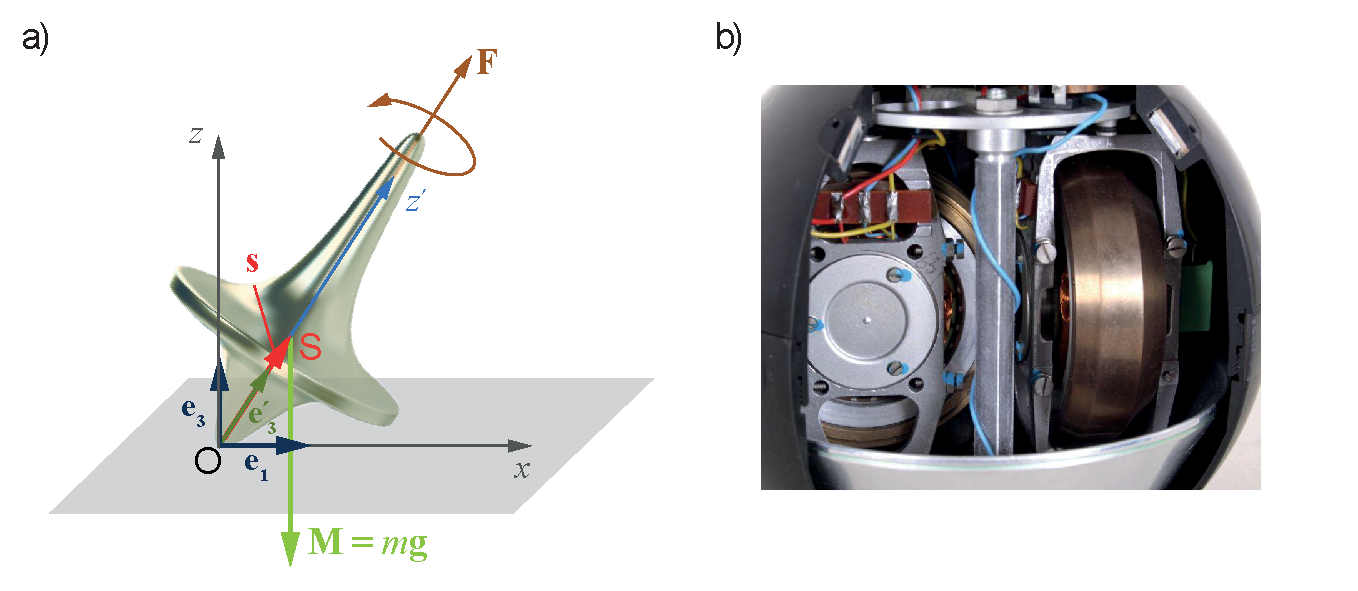
\includegraphics[width=\textwidth]{SchwererKreisel01.pdf}
  %\caption[Schwerer symmetrischer Kreisel.]{Beispiele eines schweren
    %symmetrischen Kreisels. a) Der Unterst�tzungspunkt (hier die Auflage auf
    %dem Boden) stimmt nicht mit dem Schwerpunkt �berein. Dadurch wirkt
    %ein Drehmoment auf den Kreisel, das die Bewegung beeinflusst. Das Drehmoment greift am Schwerpunkt an und zeigt in die Papierebene hinein. b) Anwendung des Prinzips des schweren Kreisels im maritimen Kreiselkompass. Einblick in einen Kreiselkompass der Firma  Ansch�tz-Raytheon.
    %}\label{abb:bew_SchwererKreisel}
%\end{figure}
\begin{figure}
  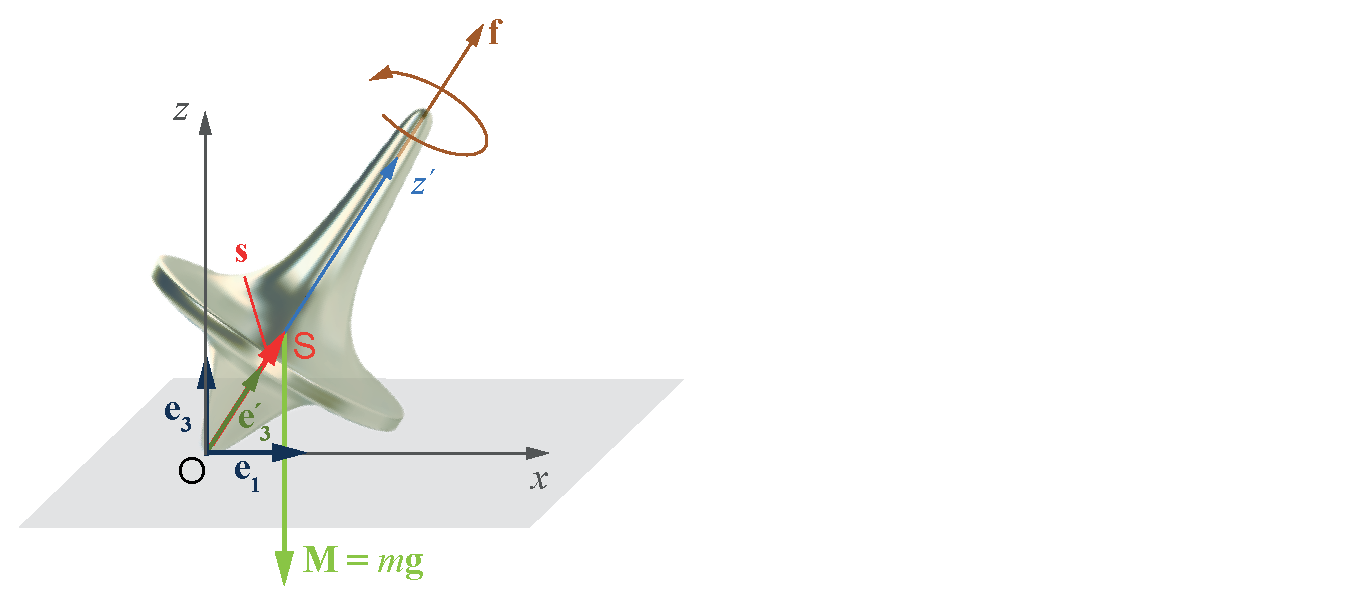
\includegraphics[width=\textwidth]{SchwererKreisel.pdf}
  \caption[Schwerer symmetrischer Kreisel.]{Beispiel  eines schweren
    symmetrischen Kreisels. Der Unterst�tzungspunkt (hier die Auflage auf
    dem Boden) stimmt nicht mit dem Schwerpunkt �berein. Dadurch wirkt
    ein Drehmoment auf den Kreisel, das die Bewegung beeinflusst. Das Drehmoment greift am Schwerpunkt an und zeigt in die Papierebene hinein.}\label{abb:bew_SchwererKreisel}
\end{figure}

Wir wollen wieder einen besonders interessanten Spezialfall betrachten. Dazu gehen wir davon aus, dass die Figurenachse $\vec{f}=\vecpeZ$,\,$\vec{\omega}$ und $\vec{L}$ parallel zueinander liegen und dies im wesentlichen auch so bleibt, weil das Drehmoment nur eine kleine �nderung der Bewegung hervorruft. Mit dieser Annahme steht das Drehmoment wegen
	\[\MD = m \, g \,\vecpeZ \times \veceZ \;\propto \;\vec{L} \times \veceZ\]
senkrecht zum Drehimpuls, da es senkrecht zur Figurenachse gerichtet ist. Die Darstellung in \figref{bew_SchwererKrPraezessionL}a verdeutlicht dies.

\begin{figure}
  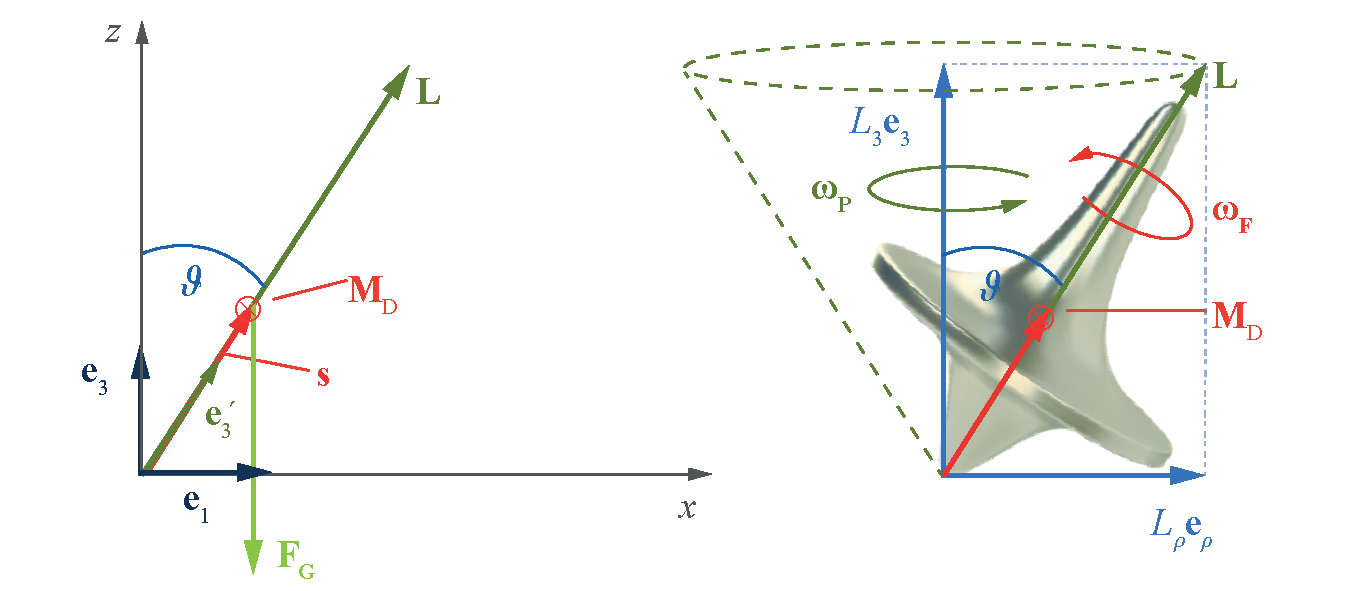
\includegraphics[width=\textwidth]{SchwererKrPraezessionL.pdf}
  \caption[Drehmoment auf einen schweren Kreisel.]{Pr�zession aufgrund eines
    Drehmoments am schweren symmetrischen Kreisel f�r den nutationsfreien
    Spezialfall, in dem der Drehimpuls $\vec{L}$, die Rotationsachse
    $\vec{\omega}$ und die Figurenachse $\vec{f}=\vecpeZ$ aufeinander liegen.
    Durch die Gewichtskraft wirkt ein Drehmoment, das senkrecht zum Drehimpuls
    liegt und dessen Richtung �ndert. Es ergibt sich eine Rotation des
    Drehimpulses um die $\veceZ$-Achse. 
		%c) Pr�zession und Nutation des schweren symmetrischen Kreisels �berlagert.
    \label{abb:bew_SchwererKrPraezessionL}}
\end{figure}
%
Das Drehmoment folgt aus
\begin{equation*}
  \MD = \vec{s} \times \vec{F}_\mathrm{G} = \left ( s \sin\vartheta\,
    \vec{e}_\varrho + s \cos \vartheta \, \veceZ \right ) \times
  (-mg)\,\veceZ = m\,g\,s\sin\vartheta \, \vec{e}_\varphi \; ,
\end{equation*}
wobei hier Zylinderkoordinaten ($\vec{e}_\varrho, \vec{e}_\varphi, \vec{e}_z = \vec{e}_3$) f�r das raumfeste Koordinatensystems $\vec{\Sigma}$
eingef�hrt wurden. Die Aufteilung des Drehimpulses erfolgt in eine Komponente parallel zur
$\veceZ$-Achse und eine senkrecht dazu. In Zylinderkoordinaten l�sst
sich das schreiben als (\figref{bew_SchwererKrPraezessionL}b)
\begin{align*}
  \vec{L} &= L_\varrho \,\vec{e}_\varrho + L_3 \,\veceZ \,,
            \intertext{woraus sich f�r die Zeitableitung ergibt}
            \frac{\D}{\D t} \vec{L} &= \dot{L}_\varrho \, \vec{e}_\varrho +  L_\varrho\,\dot{\vec{e}}_\varrho + \dot{L}_3 \,\veceZ
                                      = \dot{L}_\varrho \,\vec{e}_\varrho +  L_\varrho \,\dot{\varphi} \, \vec{e}_\varphi + \dot{L}_3 \,\veceZ \\
          &\overset{!}{=} \MD = m\,g\,s\, \sin\vartheta \, \vec{e}_\varphi = \text{const} \, \vec{e}_\varphi\; .
\end{align*}
Daraus liest man sofort wegen $\D (L^2) / \D t = 2\,\vec{L}\,\D \vec{L}/\D t $ ab, dass auch $ L = \D \left| \vec{L}\right|/\D t = 0$ und 
\begin{equation}
  \dot{\varphi} = \frac{m \,g \,s \,\sin\vartheta}{L_\varrho} = \frac{m\, g\, s\, \sin\vartheta}{\left | \vec{L} \right | \sin\vartheta} = \frac{m\, g\, s}{\left | \vec{L} \right |} = \frac{m\, g\, s}{J_3 \,\omega_F} = \con  = \omega_P \label{eq:bew_SchwererKr01}
\end{equation}
gelten. Hier ist wobei $\omega_\text{F}$ die Kreisfrequenz der schnellen Drehbewegung um die
Figurenachse. Die Komponenten $L_\varrho$ und $L_3$ und damit der Betrag
des Drehimpulses sind, wie es sein muss, konstant.
Im betrachteten Spezialfall folgt die Figurenachse der Bewegung des
Drehimpulses und im Ergebnis erh�lt man eine Drehung des schweren symmetrischen
Kreisels mit der Winkelgeschwindigkeit
\begin{equation}
  \omega_P = \frac{m\, g\, s}{J_3\,\omega_\text{F}} \label{eq:bew_SchwererKr02}
\end{equation}
um die $\veceZ$-Achse. Diese Bewegung hei�t \emph{Pr�zession}\index{Pr�zession} und $\omega_P$ wird
\emph{Pr�zessionskreisfrequenz} oder oft auch kurz \emph{Pr�zessionsfrequenz}\index{Pr�zessionsfrequenz} genannt. Ausf�hrlicher, insbesondere �ber den hier
gew�hlten Spezialfall hinaus, erfolgt die Betrachtung in
\kap{bew_SchwererSymmKr}. Daf�r f�hren wir jedoch zun�chst den
Lagrange-Formalismus f�r den starren K�rper ein.

\subsection{Lagrange-Formalismus f�r einen Kreisel}\index{Lagrange-Formalismus} \label{kap:bew_Lagrange_StarrerK}

Der Lagrange-Formalismus f�r starre K�rper folgt in allen Punkten den in 
\kap{bew_lagrange_formalism} dargelegten Grundz�gen f�r Massepunkte.
Als besondere Zwangsbedingung kommt hinzu,
dass sich die Massepunkte des Systems nicht unabh�ngig voneinander
bewegen k�nnen.
Die einzigen verbleibenden Freiheitsgrade sind diejenigen,
die bereits durch die Betrachtung der kinetischen Energie in
\kap{bew_StarrerK_kin_Energie} offensichtlich wurden, n�mlich
die Position des Schwerpunkts $\vec{R}_S$ und die aktuelle Rotation
$\vec{\xi}$ des K�rpers.
Dabei entspricht die Rotation $\vec{\xi}$ drei
Freiheitsgraden und kann beispielsweise durch die Angabe einer Drehachse (2
Koordinaten) und eines Drehwinkels (1 Koordinate) oder durch die drei
Euler-Winkel beschrieben werden.
Insgesamt haben wir es also bei einem
freien starren K�rper mit sechs Freiheitsgraden zu tun.
Diese k�nnen
durch zus�tzliche Zwangsbedingungen (\zb Einspannen am Schwerpunkt und
somit $\vec{R}_S = \conv$) weiter eingeschr�nkt werden.

Gibt es keine weiteren Einschr�nkungen, sind geeignete generalisierte
Koordinaten bereits durch $\vec{R}_S$ und $\vec{\xi}$ gegeben.
F�r den allgemeinen freien starren K�rper erh�lt man die kinetische
Energie nach Gleichungen \eqref{eq:bew_Kin_Energie_starrerK} und
\eqref{eq:bew_Trot_starrerK}, n�mlich
\begin{equation}
  T = T_\mathrm{trans} + T_\mathrm{rot}
  = \frac{1}{2} M\,{\vec{V}_S}^2 +  \frac{1}{2} \vec{\omega}^T \underline{\vec{\Theta}} \,\vec{\omega} 
  \label{eq:bew_Lagrange_starrerK1}
\end{equation}
mit $\vec{V}_S = \dot{\vec{R}}_S$ und $\vec{\omega} = \dot{\vec{\xi}}$.

Das Potential kann im allgemeinen Fall sowohl von der Position des
Schwerpunkts $\vec{R}_S$ als auch der Lage des K�rpers $\vec{\xi}$
abh�ngen, sodass man die allgemeine Lagrange-Funktion
\begin{equation}
  \mathcal{L}(\vec{R}_S,\vec{\xi},\vec{V}_S,\vec{\omega}) =
  T(\vec{V}_S,\vec{\omega}) - U(\vec{R}_S,\vec{\xi})
= \frac{1}{2} M\,{\vec{V}_S}^2 +  \frac{1}{2} \vec{\omega}^T \underline{\vec{\Theta}} \,\vec{\omega} - U(\vec{R}_S,\vec{\xi})
\end{equation}
erh�lt.
In vielen Anwendungen ist man jedoch wieder nicht an der Bewegung
des Schwerpunkts interessiert.
Das gilt insbesondere f�r F�lle, in denen
der starre K�rper keine Translation ausf�hrt.
In diesem Fall reduziert sich die Lagrange-Funktion auf
\begin{equation}
  \mathcal{L}(\vec{\xi},\vec{\omega}) = T(\vec{\omega}) - U(\vec{\xi}) =
  \frac{1}{2} \,\vec{\omega}^T \underline{\vec{\Theta}} \,\vec{\omega} - U(\vec{\xi})
  ~.   \label{eq:bew_Lagrange_starrerK2}
\end{equation}
F�r viele Anwendungen stellen die in \kap{bew_EulerWinkel}
eingef�hrten Euler-Winkel eine geeignete und elegante Darstellung bereit.
Mit der Annahme, dass das k�rperfeste Koordinatensystem ein Hauptachsensystem
ist, betr�gt die kinetische Energie
\begin{equation*}
  T(\vec{\omega}) = \frac{1}{2} \lk J_1 \omega_1'^2 + J_2 \omega_2'^2
    + J_3 \omega_3'^2 \rk
\end{equation*}
\bzw mithilfe der Euler-Winkel \eqref{eq:bew_EulerWinkel} ausgedr�ckt
\begin{equation*}
  T(\vec{\omega}) = \frac{1}{2} \left ( J_1\,(\dot{\varphi} \sin\vartheta \sin
    \psi + \dot{\vartheta} \cos\psi)^2 + J_2 \,(\dot{\varphi} \sin\vartheta \cos
    \psi - \dot{\vartheta} \sin\psi)^2
    + J_3 \,(\dot{\varphi} \cos\vartheta + \dot{\psi})^2 \right ) \,. 
\end{equation*}
Die Lagrange-Funktion lautet dann
\begin{multline}
  \mathcal{L}(\varphi,\vartheta,\psi,\dot{\varphi},\dot{\vartheta},\dot{\psi})
  = \frac{1}{2} \Bigl ( J_1 (\dot{\varphi} \sin\vartheta \sin
    \psi + \dot{\vartheta} \cos\psi)^2 + J_2 (\dot{\varphi} \sin\vartheta \cos
    \psi - \dot{\vartheta} \sin\psi)^2 \\
    + J_3 (\dot{\varphi} \cos\vartheta + \dot{\psi})^2 \Bigr )
  -U(\varphi,\vartheta,\psi) ~ .  \label{eq:bew_Lagrange_starrerK3}
\end{multline}

\subsection{Dynamik des schweren symmetrischen Kreisels}\index{Kreisel!schwerer symmetrischer} \label{kap:bew_SchwererSymmKr}

Eine typische Anwendung, die den Vorteil des Lagrange-Formalismus sichtbar
macht, ist der symmetrische schwere Kreisel aus
\figref{bew_SchwererKreisel}.
Ausgedr�ckt in den Euler-Winkeln lautet seine Lagrange-Funktion mit $J_{12}=J_1=J_2$
\begin{equation}
  \mathcal{L} = \frac{J_{12}}{2}\, \left ( \dot{\varphi}^2 \sin^2\vartheta + \dot{\vartheta}^2
\right ) + \frac{J_3}{2}\, \left (\dot{\varphi} \cos\vartheta + \dot{\psi}
\right )^2 - m\,g\,s\,\cos{\vartheta} \,.  \label{eq:bew_Lagrange_starrerK4}
  \end{equation}
  Die Koordinaten $\varphi$ und $\psi$ sind zyklisch (das Potential h�ngt nur von $\vartheta$ ab)
  und f�hren direkt auf die beiden Erhaltungsgr��en
  \begin{align*}
    p_\psi &= \frac{\partial \mathcal{L}}{\partial \dot{\psi}} =
    J_3 \left ( \dot{\varphi} \cos\vartheta + \dot{\psi} \right )
             = J_3 \,\omega_3 = \con
    \intertext{und}
    p_\varphi &= \frac{\partial \mathcal{L}}{\partial \dot{\varphi}}
    = J_{12} \, \dot{\varphi} \sin^2\vartheta + J_3 \left ( \dot{\varphi}
                \cos\vartheta + \dot{\psi} \right ) \cos\vartheta =
    J_{12}\, \dot{\varphi} \sin^2\vartheta + J_3\,\omega_3 \cos\vartheta = \con\,.
  \end{align*}
  Aus ihnen lassen sich die Zeitentwicklungen der Winkel $\varphi$ und $\psi$ zu
  \begin{align}
	\begin{split}
    \dot{\varphi} &= \frac{p_\varphi - J_3 \, \omega_3 \cos\vartheta}{J_{12} \sin^2
    \vartheta} ~ , \\ 
    \dot{\psi} &= \omega_3 - \frac{p_\varphi - J_3 \, \omega_3 \cos\vartheta}
    {J_{12} \sin^2 \vartheta} \cos\vartheta ~ 
	\end{split} \label{eq:bew_Lagrange_starrerK4a}
  \end{align}
  berechnen. Eine weitere Erhaltungsgr��e ist die Gesamtenergie $E = T + U$.
  Setzt man in diese das Wissen \eqref{eq:bew_Lagrange_starrerK4a} �ber $\dot{\varphi}$ und $\dot{\psi}$ 
	 ein, erh�lt man
  \begin{align}
    E &= \frac{J_{12}}{2} \,\left ( \dot{\varphi}^2 \sin^2\vartheta
      + \dot{\vartheta}^2 \right )
    + \frac{J_3}{2}\, \left (\dot{\varphi} \cos\vartheta + \dot{\psi} \right )^2
    + mg s \cos{\vartheta} \nonumber \\
    &=  \frac{J_{12}}{2} \,\dot{\vartheta}^2 + \underbrace{\frac{\left ( p_\varphi - J_3 \,\omega_3\,
        \cos\vartheta \right )^2}{2 J_{12} \,\sin^2\vartheta}
      + \frac{J_3}{2}\, \omega_3^2 + m\,g\,s\,\cos{\vartheta}}_{U_\mathrm{eff}(\vartheta)}
      = \frac{J_{12}}{2}\, \dot{\vartheta}^2 + U_\mathrm{eff}(\vartheta) ~.
			\label{eq:bew_Lagrange_starrerK4b}
  \end{align}
Die Energie h�ngt nur noch von $\dot{\vartheta}$ und einem effektiven Potential $U_\mathrm{eff}(\vartheta)$ ab, das wiederum eine Funktion nur von $\vartheta$ ist.
Dieses Potential hat f�r die Kreiselparameter
$m=\SI{1}{\kg}$ (Masse), $J_3 = \SI{0.6}{\kg\metre\squared}$, $J_{12} = \SI{0.4}{\kg\metre\squared}$ (Tr�gheitsmomente), $\omega_3 = \SI{1}{\per\s}$ (Rotationskreisfrequenz der Figurenachse), $s=\SI{20}{\centi\metre}$ (Abstand des Auflagepunktes zum Schwerpunkt) und dem
Verh�ltnis der zyklischen \anf{Impulse}
		\[\frac{p_\varphi}{p_\psi} = \frac{p_\varphi}{J_3\,\omega_3} = \frac{1}{3}
	\] die in \figref{bew_SchwererKrPot} dargestellte Form.
  Daraus gewinnt man eine isolierte Bewegungsgleichung f�r $\vartheta$,
  \begin{equation}
    J_{12} \ddot{\vartheta} = \frac{\left ( p_\varphi - J_3\, \omega_3
        \cos\vartheta \right )^2}{J_{12} \sin^3\vartheta} \cos\vartheta
    -J_3\, \omega_3 \,\frac{p_\varphi-J_3\, \omega_3\cos\vartheta}{J_{12}\sin\vartheta}
    + m\,g\,s\,\sin\vartheta \; . \label{eq:bew_Lagrange_starrerK4c}
  \end{equation}
  Diese Gleichung kann im Allgemeinen nur numerisch gel�st werden.
  F�r verschiedene Gesamtenergien $E$, die durch die verschiedenen Linien im Potentialdiagramm dargestellt 
	sind, haben wir die Bewegungsabl�ufe im \mscr{} \mlbewref{SchwererKreiselPraez02.m}
  f�r den Winkel des Drehimpulses zur $z$-Achse (dem Euler-Winkel $\vartheta$) beispielhaft berechnet
  und in \figref{bew_SchwererKrPtheta} dargestellt. 

\begin{figure}
\begin{minipage}{\textwidth}
\leftfigure{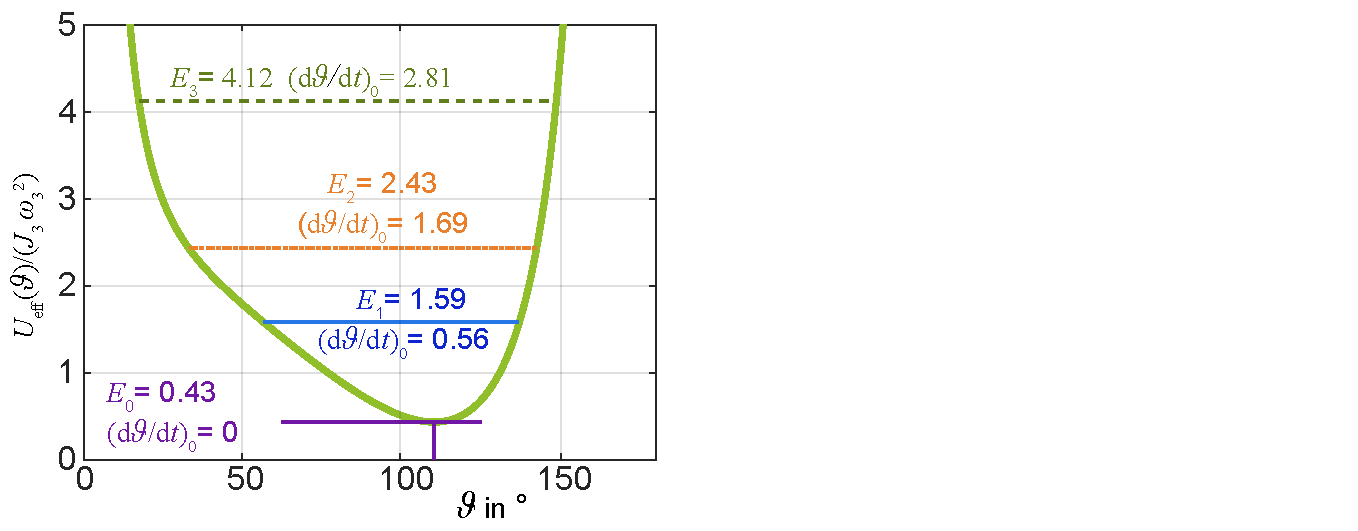
\includegraphics[width=0.9\textwidth]{SchwererKrPot.pdf}}%
\hspace{\fill}
\rightfigure{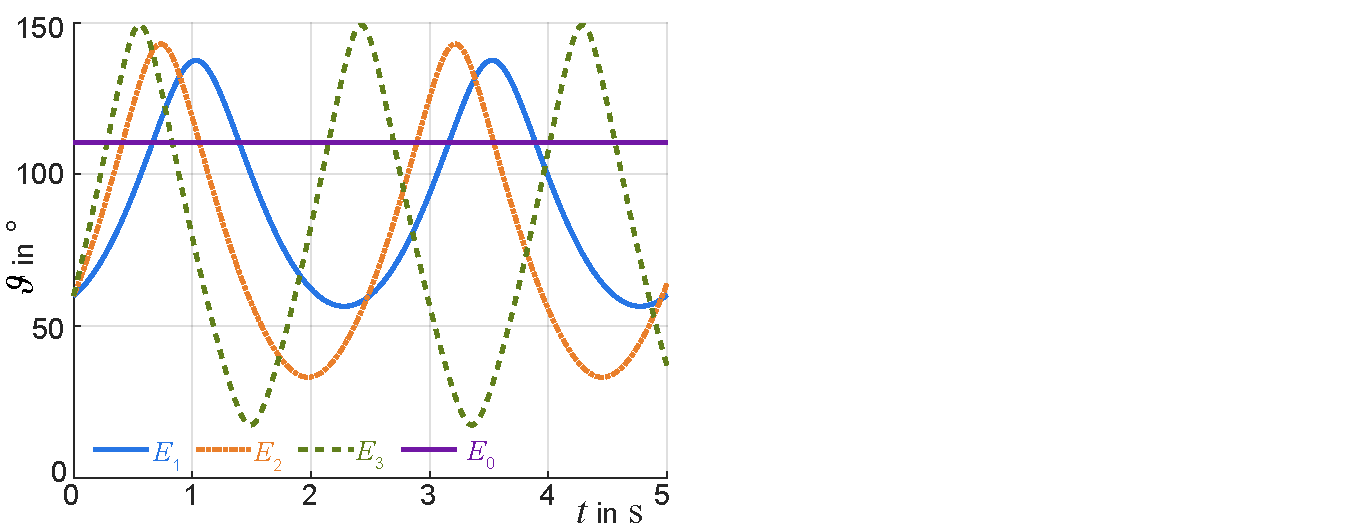
\includegraphics[width=0.9\textwidth]{SchwererKrPtheta.pdf}}
\leftcaption[Effektives Potential eines schweren Kreisels.]{Effektives Potential eines schweren Kreisels als Funktion des Euler-Winkels $\vartheta$.} \label{abb:bew_SchwererKrPot}
\rightcaption[Dynamik des Euler-Winkels $\vartheta$ beim schweren Kreisel.]{Dynamik des Euler-Winkels $\vartheta$ beim schweren Kreisel f�r verschiedene Energien (Werte aus Abb.\ \figref{bew_SchwererKrPot}).}\label{abb:bew_SchwererKrPtheta}
\end{minipage}
\end{figure}

  Man erkennt deutlich, wie die Bewegung am linken und rechten Rand des
  Potentials umkehrt. Der Neigungswinkel des Kreisels vollf�hrt eine periodische
  Bewegung zwischen diesen Extremwerten, die bei geringer Energie noch nahezu harmonisch ist,
  f�r h�here Energien aufgrund der Steilheit des Potentials aber in nick�hnliche Bewegungen �bergeht.
  Da der Drehimpulsvektor in diesem Fall nicht mit der Figurenachse und der Richtung der Winkelgeschwindigkeit $\vec{\omega}$ 
  �bereinstimmt, ist die Wirkung des Drehmoments mit einer Nutation\index{Nutation} �berlagert
  und die gesamte Bewegung des Kreisels inklusive der Ver�nderungen von $\psi$ und $\varphi$ relativ kompliziert.
	
\subsubsection{Schwerer Kreisel ohne Nutation}\label{kap:bew_SchwererSymmKr_O_Nutation}

  Wir k�nnen zun�chst f�r sehr geringe Energien diese zus�tzliche Nutationsbewegung vernachl�ssigen und erhalten  eine reine Pr�zession\index{Pr�zession!reine}%
  \footnote{Mitunter wird diese Pr�zession ohne begleitende Nutation auch \textit{regul�re Pr�zesssion}\index{Pr�zession!regul�re} oder \textbf{astronomische Pr�zession} genannt. Letzterer Begriff wird in \kap{bew_praez_erde} klarer werden. Zur unterschiedlichen Verwendung von Begrifflichkeiten siehe auch die Bemerkungen in \kap{bew_Kreisel_kraeftefrei}.},
  also eine Drehung der Drehimpulsachse des Kreisels im Raum durch die Wirkung
  des Drehmoments. Diese erh�lt man exakt als Spezialfall, wenn die
  Anfangsbedingungen so gew�hlt werden, dass $\vartheta(t=0)$ sich gerade im
  Minimum des effektiven Potentials befindet und damit die Anfangswinkelgeschwindigkeit $\dot{\vartheta}(t=0) = 0$ ist. 
  Das Ergebnis f�r diesen Spezialfall ist in \figref{bew_SchwererKrEuler_o_N} dargestellt,
  hierbei ergibt sich eine stabile
  Neigung $\vartheta$ der Figurenachse. Diese dreht sich jedoch durch
  das wirkende Drehmoment im Raum, wie an der linearen Zunahme von $\varphi$
  zu sehen ist. Dabei f�hrt der Kreisel eine Eigendrehung mit der
  Frequenz $\dot{\psi}$ um die Figurenachse aus.
\begin{figure}
\begin{minipage}{\textwidth}
\leftfigure{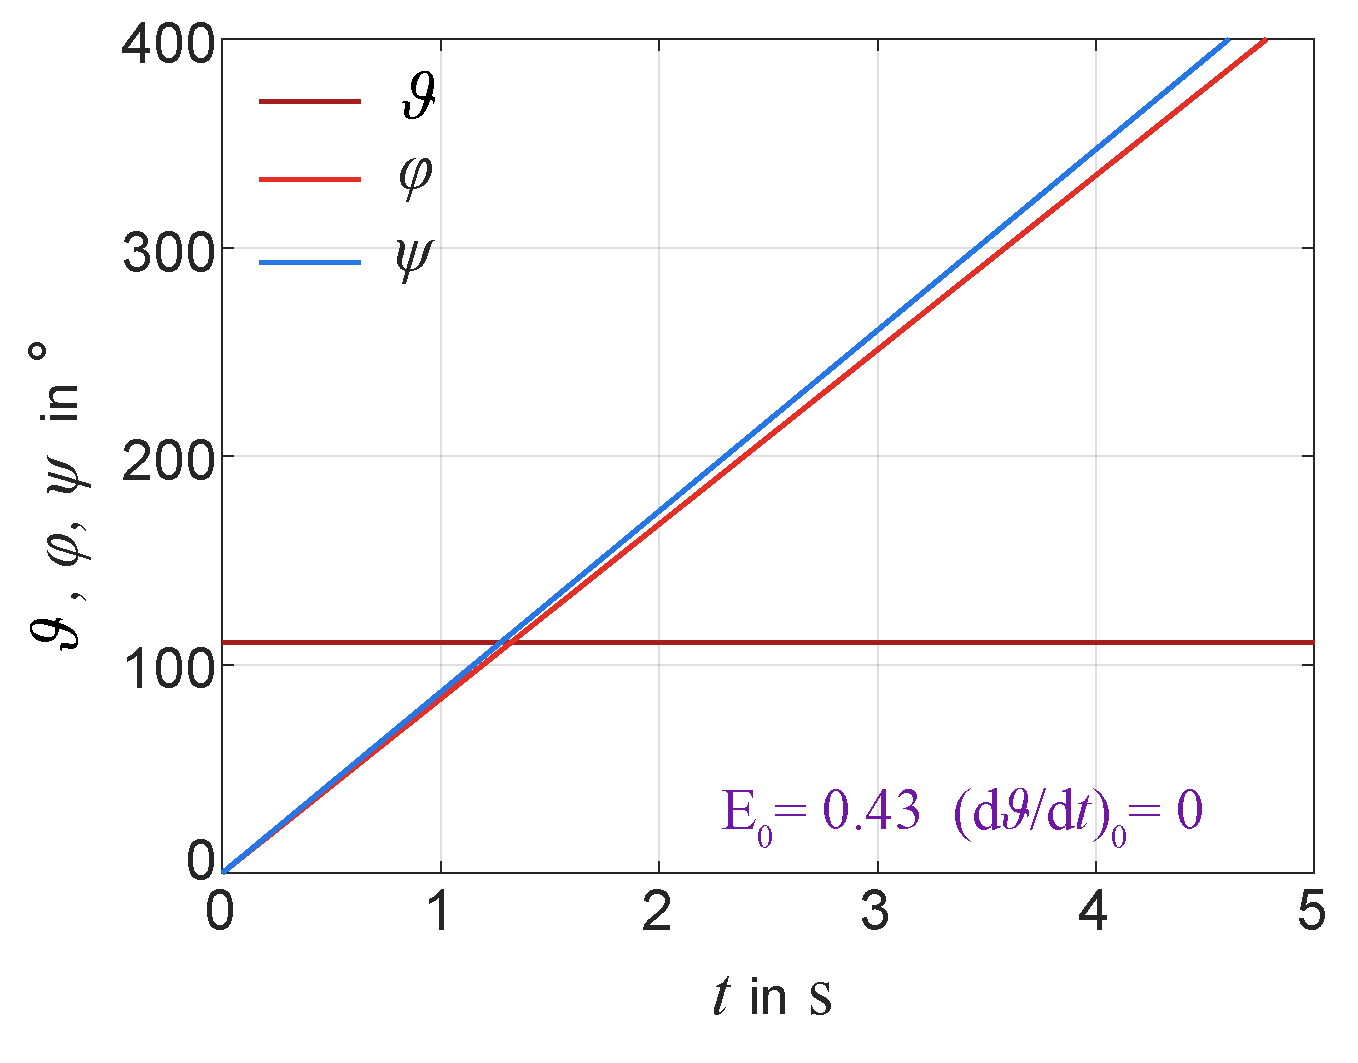
\includegraphics[width=0.45\textwidth]{SchwererKrEulerWohneN.pdf}}%
\hspace{\fill}
\rightfigure{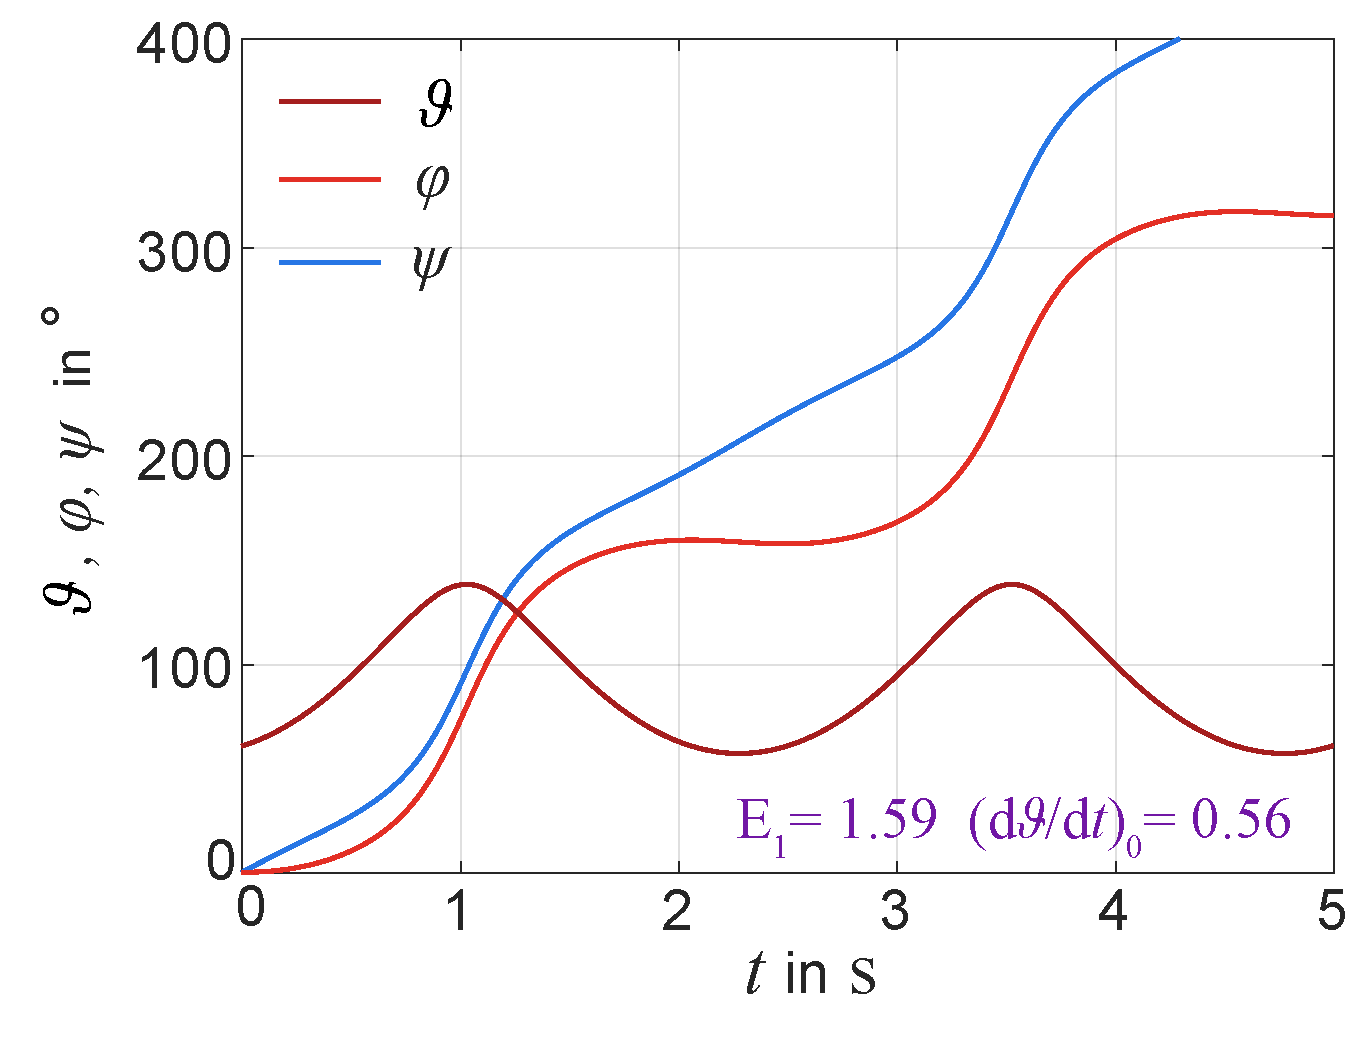
\includegraphics[width=0.45\textwidth]{SchwererKrEulerWmitN.pdf}}
\leftcaption[Dynamik der Euler-Winkel ohne Nutation.]{Dynamik der Euler-Winkel beim schweren Kreisel ohne Nutation.}\label{abb:bew_SchwererKrEuler_o_N}
\rightcaption[Dynamik der Euler-Winkel mit Nutation.]{Dynamik der Euler-Winkel beim schweren Kreisel mit Nutation.  Man erkennt am Winkel $\vartheta$ die Nickbewegungen der Nutation, ebenso ist die Eigendrehung um die Figurenachse von der Nutation �berlagert.} \label{abb:bew_SchwererKrEuler_m_N}
\end{minipage}
\end{figure}

\subsubsection{Schwerer Kreisel mit Nutation}\label{kap:bew_SchwererSymmKr_M_Nutation}

F�r den allgemeineren Fall mit  $\dot{\vartheta}(t=0) \neq 0$ ist der Bewegungsablauf im \mscr{} \mlbewref{SchwererKreiselSim.m} berechnet und in \figref{bew_SchwererKrEuler_m_N} dargestellt. Deutlich erkennbar sind die Nickbewegungen sowohl im Winkel $\vartheta$ als auch im Winkel $\varphi$.\\
Die Pr�zession und die Nutation des Erdkreisels spielen, wie bereist erw�hnt, 
in der Astronomie und der Himmelsmechanik (Band II, Kapitel 3) 
eine wichtige Rolle.
Da die Erde nahezu ein Rotationsellipsoid ist, bewirkt seine �quatorwulst, dass die Gezeitenkr�fte von Mond und Sonne ein Drehmoment erzeugen, das die Erdachse aufzurichten versucht und zur Pr�zession der Erdachse f�hrt (sogenannte \emph{lunisolare Pr�zession})\index{Pr�zession!lunisolare|textbf}.
Die Erdachse bewegt sich dadurch auf einem Pr�zessionskegel um eine Achse, die in etwa rechtwinklig auf der Ebene der Erdbahn um die Sonne steht. Der (nahezu) konstante Winkel zwischen der Erdachse und der Achse des Kegels ist die sogenannte Schiefe der Ekliptik; diese betr�gt derzeit etwa $23.44\degree$. Ein voller Umlauf dieser Pr�zessionsbewegung der Erdachse dauert etwa $\SI{25700}{}$ bis $\SI{25850}{}$ Jahre.\footnote{Die Beitr�ge zur astronomischen Pr�zession sind vor allem 
die Gezeitenkr�fte von Mond und Sonne, aber auch Beitr�ge anderer Planeten und Effekte der Allgemeinen Relativit�tstheorie.
Alle diese Betr�ge sind nicht konstant. Daher kann die Pr�zessionsperiode bisher nur auf etwa ein Jahrhundert angegeben werden.} (siehe \kap{bew_praez_erde}).


\clearpage
\section {Beispiele und Anwendungen zur Mechanik des starren K�rpers}\label{
kap:bew_anwendungen_II}

\subsection{Das physikalische Pendel und die Pendeluhr} \index{Pendel!physikalisches|textbf}\index{Pendel!Uhrenpendel} \label{kap:bew_pendel_phys}

Wir wollen nun mit dem Handwerkszeug von \kap{bew_starrer_koerper} einige Alltagsprobleme angehen.
Als erstes wollen wir die alte Pendeluhr aus Familienbesitz untersuchen.
In \probref{bew_traegheitsmomente} hatten wir ja schon das Gesamttr�gheitsmoment bez�glich der Pendelachse als Funktion der Position der Scheibenmasse und des Schiebereglers berechnet.
Bevor wir die Pendelperiode in Abh�ngigkeit dieser beider Parameter berechnen, soll zun�chst die Pendelgleichung eines beliebigen an einem Drehpunkt $O$ aufgeh�ngten starren K�rpers berechnet werden.
Wir betrachten dazu \figref{bew_PhysPendel}.

\begin{figure}
\begin{minipage}{\textwidth}
\leftfigure{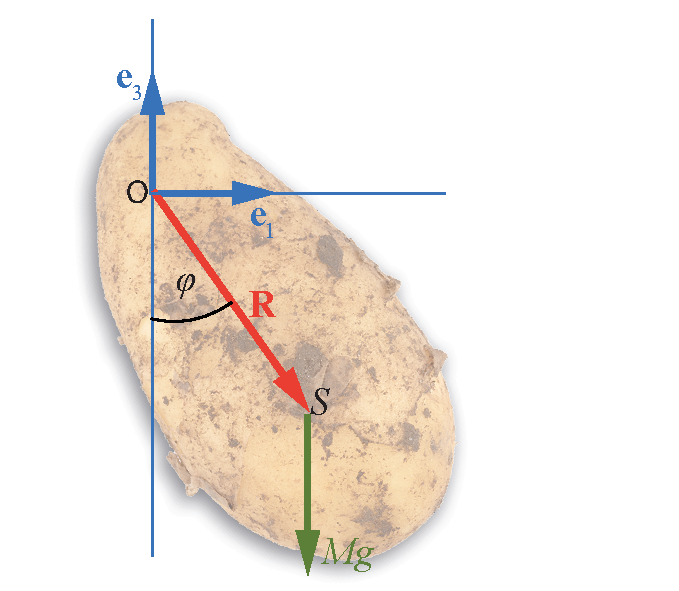
\includegraphics[width=0.5\textwidth]{PhysPendel.pdf}}%
\hspace{\fill}
\rightfigure{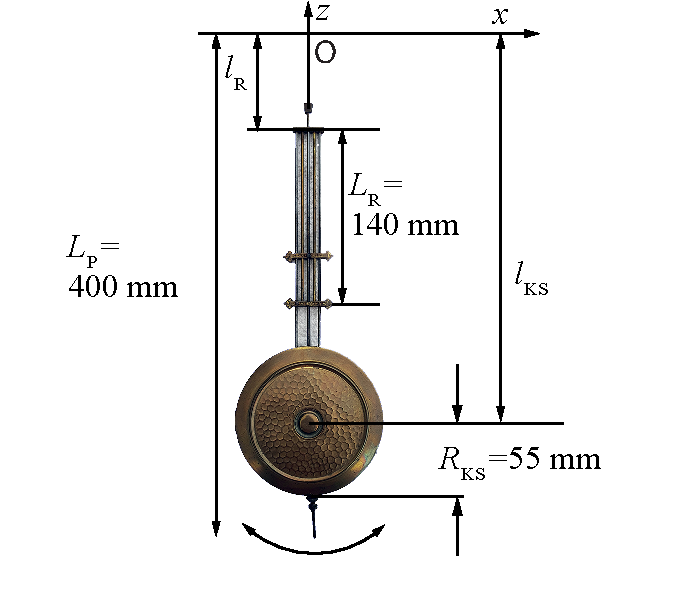
\includegraphics[width=0.5\textwidth]{Pendeluhr02.pdf}}
\leftcaption{Allgemeine Form eines physikalischen Pendels.} \label{abb:bew_PhysPendel}
\rightcaption[Realisierung des physikalischen Pendels als Pendeluhr.]{Realisierung des physikalischen Pendels als Pendeluhr.}\label{abb:bew_Pendeluhr02}
\end{minipage}
\end{figure}

Der starre K�rper (das physikalische Pendel) ist in $O$ aufgeh�ngt,
%/fixiert, => dann fehlte der rot. Fhg
der Schwerpunkt befindet sich in $S$.
Der K�rper habe das Tr�gheitsmoment $J_S$ bez�glich seines Schwerpunktes.
Dann k�nnen wir den Steinerschen Satz \eqref{eq:bew_SteinerSatz} anwenden und erhalten das Tr�gheitsmoment bez�glich der Drehachse $\veceY$ zu
        \begin{align*}
            J \, = \,J_S \,+ \,M\,R^2 \,,
        \end{align*}
worin $R$ der senkrechte Abstand der Drehachse zum Schwerpunkt ist. Das Drehmoment bez�glich der Achse $\veceY$ ist gegeben durch
        \begin{align*}
            \vec{M}_\text{D} &= \vec{R}\times \vec{F}_\text{G} = -M\,g\,\vec{R}\times\veceZ ~~\text{\bzw} ~~ {M}_\text{D} = -M\,g\,R\,\sin\varphi\,\veceY \,.
        \end{align*}
Nach dem Drehimpulssatz \eqref{eq:bew_DrehimpulsSatz} gilt
        \begin{align*}
           \frac{\D}{\D t}\,\lk J\,\omega_2\rk =  -M\,g\,R\,\sin\varphi \,,
        \end{align*}
worin $\omega_2$ die Rotationsfrequenz um die Achse $\veceY$ ist. Da $J$ konstant ist, k�nnen wir mit $\frac{\D \omega_2}{\D t} = \frac{\D}{\D t} \dot{\varphi} = \ddot{\varphi}$ schreiben:
        \begin{align}
            \ddot{\varphi} +\frac{M\,g\,R}{J} \,\sin\varphi = 0 \,. \label{eq:bew_PhysPendel01}
        \end{align}
Das ist eine Schwingungsgleichung, die f�r nicht zu gro�e Auslenkungen $\varphi$ in die Gleichung f�r den harmonischen Oszillator �bergeht:
        \begin{align}
            \ddot{\varphi} +\frac{M\,g\,R}{J}\,\varphi = 0 \,. \label{eq:bew_PhysPendel02}
        \end{align}
Hieraus berechnet sich die Schwingungsperiode des physikalischen Pendels zu
        \begin{align}
            T_\text{P} = 2\pi\sqrt{\frac{J}{M\,g\,R}} \,.\label{eq:bew_PhysPendel03}
        \end{align}
Die Schwingungsperiode des physikalischen Pendels ist also gegeben durch die Wurzel aus dem Quotienten von Tr�gheitsmoment und Drehmoment des K�rpers bezogen jeweils auf den Aufh�ngungspunkt. Da $R$ der Abstand des Schwerpunktes von der Aufh�ngung ist, haben wir f�r unsere Pendeluhr bei festgehaltenem Schieberegler und ver�nderlicher Pendelscheibe $l_\text{KS}$ also eine Abh�ngigkeit
\begin{align}
    T_\text{P}\lk l_\text{KS}, l_\text{R}\rk = 2\pi\sqrt{\frac{J\lk l_\text{KS}, l_\text{R}\rk}{M\,g\,R\lk l_\text{KS},l_\text{R}\rk}} \,, \label{eq:bew_PhysPendel04}
\end{align}
die wir im \mscr{} \mlbewref{Pendeluhr.m} berechnet und in \figref{bew_Pendeluhr03} f�r verschiedene Schiebereglerpositionen $l_\text{R}$ dargestellt haben. Man erkennt in \figref{bew_Pendeluhr03}, dass man eine hohe Einstellgenauigkeit hat.
Eine �nderung der Scheibenposition von $\SI{1}{\milli\metre}$ �ndert die Pendelperiode um \ca$\SI{1}{\milli\s}$,
die �nderung des Schiebereglers um $\SI{1}{\milli\metre}$ sogar nur um $\SI{0.1}{\milli\s}$.
Diese hohe Einstellgenauigkeit ist aber auch erforderlich,
denn bei einer Tagesl�nge von $\SI{86400}{\s}$
erzeugt eine Periodenabweichung von $\SI{0.5}{\milli\s}$
ein Nach- \bzw Vorgehen von \ca$\SI{45}{\s}$ pro Tag. 

\begin{figure}
  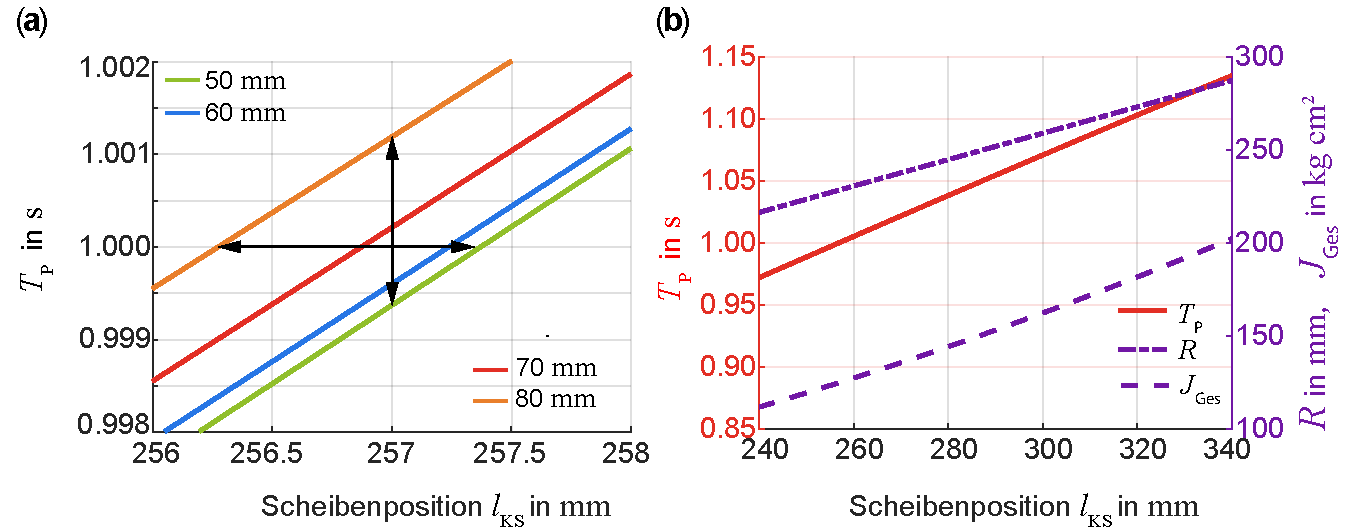
\includegraphics[width=\textwidth]{Pendeluhr03.pdf}
  \caption[Periodendauer einer Pendeluhr von den Einstellungen.]{Periodendauer einer Pendeluhr. \fa Abh�ngigkeit von den Einstellungen $l_\text{KS}$ (Abszisse) und $l_\text{R}$ (Parameter) und \fb Abh�ngigkeit vom Gesamtr�gheitsmoment $J_\text{Ges}$ und vom Abstand des Schwerpunkts $R$ von der Pendelaufh�ngung �ber einen gr��eren Bereich der Position der Pendelscheibe.}
    \label{abb:bew_Pendeluhr03}
\end{figure}

Wie man ferner erkennt, ist in guter N�herung
(aufgrund der Konstruktion (Massenverteilung) der Pendeluhr)
in der Umgebung der Normalstellung $T_\text{P} = \SI{1}{\second}$
ein linearer Zusammenhang $T_\text{P} =  C \,l_\text{KS}$ gegeben.
Das bedeutet aber auch, dass wegen $l_\text{KS} = l_0\lk 1+\alpha\,\Delta T\rk$
mit $\alpha = \SI{18.4e-6}{\per\K}$ als W�rmeausdehnungskoeffizient f�r Messing
die Uhr ungef�hr eine Temperaturabh�ngigkeit von
        \begin{align*}
            \frac{\Delta T_\text{P}}{\Delta T} &= C\,l_0\,\frac{\d}{\d T}\,\lk 1+\alpha\,\Delta T \rk = C\,l_0\,\alpha
        \end{align*}
hat. Bei einer Zimmertemperatur�nderung von $20\degree$ bedeutet das eine Periodenver�nderung von
        \begin{align*}
            \frac{\Delta T_\text{P}}{{T_\text{P}}_0} = \alpha\,\Delta T \approx \SI{4e-4}\, = \,0.04\%
        \end{align*}
�ber einen Tag mit $\SI{86400}{\second}$ hinweg summiert sich das auf $\approx \SI{35}{\second}$ auf,
sodass die Uhr bei niedrigeren Temperaturen nach 10 Tagen rund 6 Minuten nachgehen kann!

\subsection{Parametrische Oszillatoren -- Verbessertes Schaukelmodell} \index{Oszillator!parametrischer}\label{kap:bew_pendulum_schaukel}

Wir wollen nun mit den Kenntnissen der Physik des starren K�rpers ein gegen�ber dem in \kap{bew_pendulum_param} gezeigten Modell des parametrischen Oszillators ein deutlich verbessertes Modell des schaukelnden K�rpers (\figref{bew_schaukel01a}b) behandeln. Dieses sollte auch besser mit unseren Beobachtungen auf einem Spielplatz �bereinstimmt.

\begin{figure}
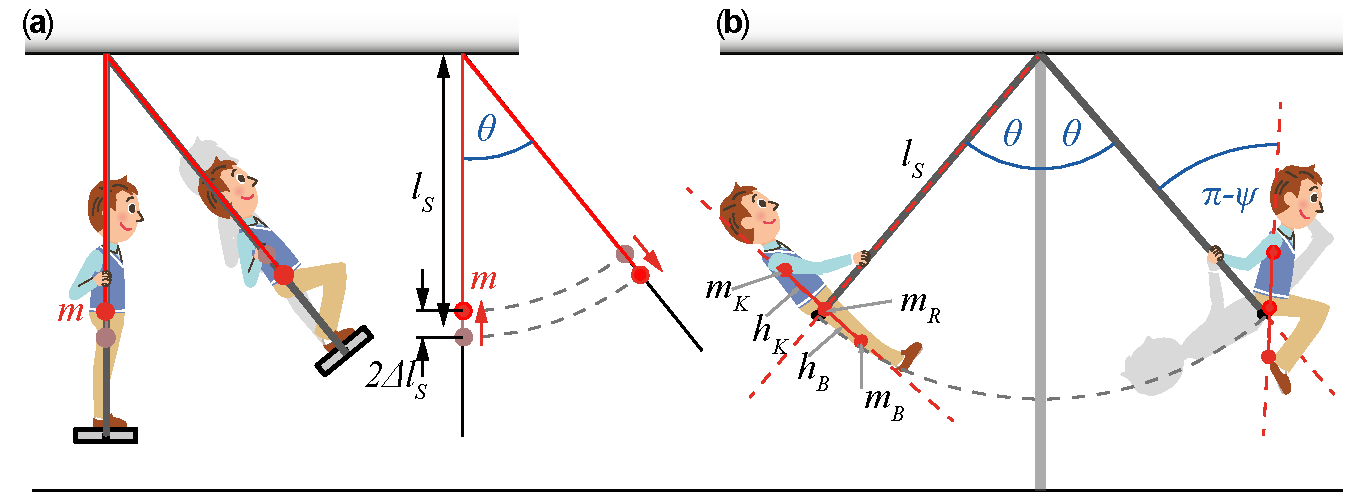
\includegraphics[width=\textwidth]{Schaukel01.pdf}
\caption[Modelle einer Schaukel.]{Modelle einer Schaukel. \fa Einfaches Massepunkt-Modell (Parametrischer Oszillator). \fb Verbessertes Schaukelmodell mit sitzender Person als starrer aber sich parametrisch-dynamisch bewegender K�rper.}
\label{abb:bew_schaukel01a}
\end{figure}

Wir nehmen zur Vereinfachung die Massen der Beine $m_\text{B}$ und des Kopfes $m_\text{K}$ als gleich an.
Die Rumpfmasse wird mit $m_\text{R}$, die Gesamtmasse mit $m_\text{g}$ bezeichnet.
Das \anf{Pumpen} der Schaukel erfolgt durch das Vor- und Zur�cklehnen des gesamten K�rpers mit einem Winkel $\psi$, einem Maximalwinkel $\psi_0$ und einer Frequenz $\omega_\text{A}$ um den Sitzpunkt.
Die Lagrange-Funktion\index{Lagrange-Funktion} ist dann gegeben durch
            \begin{align}
                \mathcal{L} = \frac{1}{2}\,J_1\,\dot{\theta}^2+\frac{1}{2}\,J_2\,\lk\dot{\theta}+\dot{\psi}\rk^2+m_\text{g}\,l_\text{S}\,g\,\cos\theta \,. \label{eq:bew_schaukel11}
            \end{align}
Mit den Massen und Geometrien von Beinen und Kopf $m_\text{g} = m_\text{R}+m_\text{K}+m_\text{B}$ , $m_\text{g} \approx m_\text{R}+2m_\text{K}$ und $h_\text{B} \approx h_\text{K} ={h}/{2}$ haben wir dann folgende Tr�gheitsmomente:
        \begin{align}
						J_1 &=m_\text{g}\,l_\text{S}^2\,~~ J_2=m_\text{K}\,\lk\frac{h^2}{4}+\frac{h^2}{4}\rk = m_\text{K}\,\frac{h^2}{2} \,. \label{eq:bew_schaukel12}
        \end{align}
Unter Ber�cksichtigung der Ann�herung der K�rperschwingung durch die rheonome Zwangsbedingung $\psi = \psi_0\,\cos\omega_\text{A} t$ ergibt sich die Lagrange-Gleichung zu (vgl.\ \kap{bew_Lagrange_I}, \cite{Ray1964})
        \begin{align}
            \lk J_1+J_2\rk\,\ddot{\theta}+m_\text{g}\,l_\text{S}\,g\,\sin\theta = -J_2\,\ddot{\psi} \,. \label{eq:bew_schaukel13}
        \end{align}
\bzw
        \begin{align}
            \ddot{\theta}+{\omega_0}^2\,\sin\theta = F_\text{A}\,\cos\omega_\text{A} t ~~~\text{mit} ~~~ {\omega_0}^2 = \frac{m_\text{g}\,l_\text{S}\,g}{J_1+J_2} ~~ \text{und} ~~ F_\text{A} = \frac{\psi_0\,{\omega_\text{A}}^2\,J_2}{J_1+J_2} \,, \label{eq:bew_schaukel14}
        \end{align}
was eine Gleichung vom Typ des getriebenen Oszillators ist (vgl. \eqref{eq:bew_pendulum02} in \kap{bew_harmon_oszillator}).
Entgegen vielen Lehrbuchdarstellungen scheinen zumindest sitzende Kinder die Schaukel als getriebenes Pendel und nicht als parametrischen Oszillator zu \anf{betreiben}.
Wir wollen aber sicherheitshalber �berpr�fen, ob dies nicht ein Ergebnis unseres zu vereinfachten Modells ist, und nehmen deshalb nun anstelle von \eqref{eq:bew_schaukel12} an, dass $m_\text{K} \neq m_\text{B}$ und auch dass $h_\text{B} \neq h_\text{K}$.
Der K�rper hat dann quasi ein spezifisches (auf $g$ bezogenes) Drehmoment $M_\text{D}$ bez�glich des Sitzpunktes, in dem wir die Rumpfmasse $m_\text{R}$ lokalisiert annehmen:\footnote{Nach unseres bisherigen Annahmen war dieses Drehmoment 0.}
        \begin{align}
            M_\text{D} = m_\text{B}\,h_\text{B}-m_\text{K}\,h_\text{K}\,. \label{eq:bew_schaukel15} 
        \end{align}
Das Tr�gheitsmoment $J_2$ ver�ndert sich nat�rlich zu
        \begin{align*}
            J_2 = m_\text{B}\,{h_\text{B}}^2+m_\text{K}\,{h_\text{K}}^2 \,,
        \end{align*}
und die Lagrange-Funktion lautet nun
        \begin{align}
				\begin{split}
        \mathcal{L} &= \frac{1}{2}\underbrace{J_1\,\dot{\theta}^2+\frac{1}{2}\,J_2\,\lk \dot{\theta}+\dot{\psi}\rk^2-l_\text{S}\,M_\text{D}\,\dot{\theta}\,\lk \dot{\theta}+\dot{\psi}\rk\,\cos\psi}_{\substack{T}} \\
				            &~~~+ \underbrace{m_\text{g}\,l_\text{S}\,g\,\cos\theta - M_\text{D}\,g\,\cos\lk\theta+\psi\rk}_{\substack{-U}}\,. 
        \end{split} \label{eq:bew_schaukel16}
				\end{align}
Der zus�tzliche Term im Potential $U$ ist leicht aus der Geometrie von \figref{bew_schaukel01}b herzuleiten, den Mischterm in der kinetischen Energie $T$ findet man nach etwas Rechnung  am einfachsten aus den kartesischen Koordinaten der drei angenommenen Massepunkte (Man benutze die Symbolic Math Toolbox von \matlab).
Wiederum unter Beachtung der rheonomen Zwangsbedingung $\psi = \psi_0\,\cos\omega_\text{A} t$ ergibt sich die nun etwas komplexere Lagrange-Gleichung f�r die generalisierte Koordinate $\theta$ zu \cite{Case1990}
  \begin{align}
     \underbrace{\lek J_1+J_2 - 2L\,M_\text{D}\,\cos\psi \rek }_{J_\text{eff}(t)} \ddot{\theta} + \underbrace{\lek 2L\,M_\text{D}\,\dot{\theta}\,\dot{\psi}\,\sin\psi \rek}_{\eta_\text{eff}(t)} + \underbrace{\lek m_\text{g}\,l_\text{S}\,g - M_\text{D}\,g\,\cos\psi \rek}_{{\omega_\text{eff}(t)}^2} \sin\theta \nonumber  \\
      \,= -\underbrace{J_2\,\ddot{\psi} - l_\text{S}\,M_\text{D}\,\sin\psi\,\dot{\psi}^2 + l_\text{S}\,M_\text{D}\,\cos\psi\,\ddot{\psi} + M_\text{D}\,g\,\sin\psi\,\cos\theta}_{F_\text{eff}(t)} 
\,.\label{eq:bew_schaukel17}
   \end{align} 
Offensichtlich ist \eqref{eq:bew_schaukel17} von der Struktur einer Schwingungsgleichung in der Koordinate $\theta$, aber mit zeitlich variablen Koeffizienten f�r das Tr�gheitsmoment $J_\text{eff}(t)$, die modifizierte, parametrische Eigenfrequenz $\omega_\text{eff}(t)$ und einem Treiberterm $F_\text{eff}(t)$ auf der rechten Seite.
F�r kleine Schaukelauslenkungen $\theta$ kann man Gl. \eqref{eq:bew_schaukel17} linearisieren und erh�lt
  \begin{align}
     \underbrace{\lek J_1+J_2 - 2L\,M_\text{D}\,\cos\psi \rek }_{J_\text{eff}(t)} \ddot{\theta} + \underbrace{\lek 2L\,M_\text{D}\,\dot{\psi}\,\sin\psi \rek}_{\eta_\text{eff}(t)} \dot{\theta} + \underbrace{\lek m_\text{g}\,l_\text{S}\,g - M_\text{D}\,g\,\cos\psi \rek}_{{\omega_\text{eff}(t)}^2} \theta \nonumber  \\
      = -\underbrace{J_2\,\ddot{\psi} - l_\text{S}\,M_\text{D}\,\sin\psi\,\dot{\psi}^2 + l_\text{S}\,M_\text{D}\,\cos\psi\,\ddot{\psi} + M_\text{D}\,g\,\sin\psi}_{F_\text{eff}(t)} 
\,.\label{eq:bew_schaukel17a}
   \end{align} 
Bevor wir an die numerische L�sung dieser Gleichungen gehen, wollen wir ihre zugrunde liegende physikalische Struktur besser verstehen. Dazu entwickeln wir f�r $\psi(t) = \psi_0\, \cos(\omega_\text{A} t)$ die Winkelfunktionen $\sin\psi$ und $\cos\psi$ in \eqref{eq:bew_schaukel17a} f�r kleine Winkel um $\psi_0$, wobei wir bei der Entwicklung nur Frequenzen bis $2\omega$ mitnehmen wollen.
Wir erhalten dann nach etwas Algebra (als �bung empfohlen, siehe auch \cite{Case1990}) die modifizierte Schwingungsgleichung  
 \begin{align}
      &\ddot{\theta} + \hat{\eta}\,\dot{\theta}+{\hat{\omega}_0}^2\,\theta = \hat{F}_\text{A}\,\cos\omega_\text{A} t \label{eq:bew_schaukel18}
 \end{align} 
mit folgenden zeitabh�ngigen Termen f�r die Reibung $\hat{\eta}$
und das Quadrat der Frequenz $\hat{\omega}_0$:
 \begin{align*}
    \hat{\eta} &= -\frac{l_\text{S}\,M_\text{D}\,\omega_\text{A}\,{\psi_0}^2}{J_0}\,\sin 2\omega_\text{A} t\, ~~~  {\hat{\omega}_0}^2 = {\omega_0}^2 + \frac{M_\text{D}\,g\,{\psi_0}^2}{4\,J_0}\,\cos 2\omega_\text{A} t \,.
 \end{align*}
Hier haben wir die folgenden Konstanten verwendet:
\begin{align*}
			{\omega_0}^2 &= \frac{M_0}{J_0}\,,~~~M_0 = m_\text{g}\,l_\text{S}\,g-M_\text{D}\,g\,\lk 1-\frac{1}{4}\,{\psi_0}^2\rk\,~~\text{und} \\
			J_0 &= J_1 + J_2 -2\,l_\text{S}\,M_\text{D}\,\lk 1-\frac{1}{4}\,{\psi_0}^2\rk \,.
\end{align*}
Auf der rechten Seite von \eqref{eq:bew_schaukel18} steht ein Anregungsterm mit der Grundfrequenz $\omega$, dessen Anregungsst�rke $F_\text{A}$ wiederum zeitlich moduliert ist,
\begin{align} 
    F_\text{A} &= \frac{\psi_0}{J_0}\lek {\omega_\text{A}}^2\,J_2 + M_\text{D}\,\lk g-{\omega_0}^2\,l_\text{S}\rk\lk 1- \frac{{\psi_0}^2}{8}\rk\rek \,.\label{eq:bew_schaukel18a}
\end{align} 
Wir erkennen aus Gleichung \eqref{eq:bew_schaukel18} sehr sch�n,
dass wir eine Kombination von parametrischer Modifikation der Schwingungsfrequenz $\hat{\omega}_0$ (und einer entsprechenden D�mpfung)
und zeitlich variabler Anregung $F_\text{A}$ haben.\\
Ergibt sich nun vielleicht durch die bessere Modellierung des schwingenden K�rpers doch ein parametrischer Oszillator? 

Wir l�sen \eqref{eq:bew_schaukel17} bis \eqref{eq:bew_schaukel19} numerisch (\mscr{} \mlbewref{Schaukel02.m}) mit den Parametern aus Tabelle \ref{tab:bew_schaukel01} und betrachten die zeitliche Entwicklung der Schaukelamplitude (\figref{bew_schaukel05}).
Deutlich ist zu erkennen, dass im Bereich geringer Auslenkungen, also zu Beginn des Schaukelns,
alle drei Rechnungen gut �bereinstimmen und das Verhalten eines getriebenen Pendels vorliegt.
Bei gr��eren Zeiten \bzw Amplituden weichen die Ergebnisse voneinander ab.
Die numerischen Rechnungen f�r die vollst�ndige Lagrange-Gleichung ergeben eine Begrenzung und sogar ein Abnehmen der Amplitude, die Reihenentwicklung zeigt dagegen ein ungest�rtes, nun auch exponentielles Anwachsen, womit wir aber den G�ltigkeitsbereich der N�herung verlassen.
Es bleibt also festzuhalten, dass das Aufschaukeln im wesentlichen der Charakteristik eines getriebenen Oszillators folgt.
Die D�mpfung \bzw Begrenzung der Schwingung resultiert aus der Tatsache, dass die Anregung mit der K�rperschwingungsfrequenz $\omega_\text{A}$ (die in Betrag und Phase in unseren Rechnungen festgehalten wurde) mit der Zeit aus der Phase der Schaukelschwingung mit der Frequenz $\omega_\text{eff}$ l�uft und damit die Schaukelschwingung d�mpft. In der Realit�t passt der Schaukelnde die Phase und Frequenz der K�rperschwingung intuitiv laufend der momentanen Eigenfrequenz der Schaukel an.

Soweit die Rechnungen. Wie kann man aber das Verhalten anschaulich verstehen?
Wir kommen noch einmal auf \eqref{eq:bew_schaukel11} zur�ck und berechnen die Zeitableitung des generalisierten Impulses, die gegeben ist durch 
        \begin{align}
            \dot{p}_\theta = \frac{\D}{\D t}\frac{\d \mathcal{L} }{\d  \dot{\theta}} = J_1\,\ddot{\theta} + J_2\,\lk \ddot{\theta}+\ddot{\psi}\rk = -m_\text{g}\,l_\text{S}\,g\,\sin\theta\,.\label{eq:bew_schaukel19}
        \end{align}
Dieser generalisierte Impuls ist zugleich der Drehimpuls bez�glich der Aufh�ngung.
Er ist offensichtlich wegen des rechten Terms in \eqref{eq:bew_schaukel19} nicht erhalten. Aber selbst wenn $\dot{p}_\theta = 0$ w�re, k�nnte zwischen den beiden Termen in \eqref{eq:bew_schaukel19} ein Drehimpulstransfer stattfinden.
Genau dieser ist zu Beginn des Schaukelns f�r die Dynamik verantwortlich.%
\footnote{Wir wollen noch erg�nzen, dass ein gewisser parametrischer Effekt durch das typische Anziehen der Beine beim Durchgang durch den tiefsten Punkt zu verzeichnen ist, den wir in unseren Rechnungen vernachl�ssigt haben. Ferner ist der Winkel des Zur�cklehnens gegen�ber der aufrechten Haltung �blicherweise merklich gr��er als der des Vorlehnens.}
        \begin{table}[h!]
          \centering
				\begin{tabular}{ l C{2cm} C{2.0cm} C{2.0cm} }
\hline
\rule{0pt}{2pt} & &  \\
              & Kind & Erwachsener\\
\rule{0pt}{2pt} & &  \\
\hline
\rule{0pt}{2pt} & & \\
              $l_\text{S}$  & $\SI{3}{\metre}$ & $\SI{4}{\metre}$ \\
              $m_\text{g}$  & $\SI{50}{\kilogram}$ & $\SI{100}{\kilogram}$ \\
              $h_\text{K}$  & $\SI{0.3}{\metre}$ & $\SI{0.55}{\metre}$ \\
              $h_\text{B}$  & $\SI{0.4}{\metre}$ & $\SI{0.75}{\metre}$ \\
              $m_\text{K}$  & $\SI{15}{\kilogram}$ & $\SI{40}{\kilogram}$ \\
              $m_\text{B}$  & $\SI{15}{\kilogram}$ & $\SI{30}{\kilogram}$ \\
              $m_\text{R}$  & $\SI{20}{\kilogram}$ & $\SI{30}{\kilogram}$ \\
\rule{0pt}{2pt} & & \\
            \end{tabular}
            \caption[Parameter der Schaukel.]{Parameter der Schaukel.}
            \label{tab:bew_schaukel01}
        \end{table}
\begin{figure}
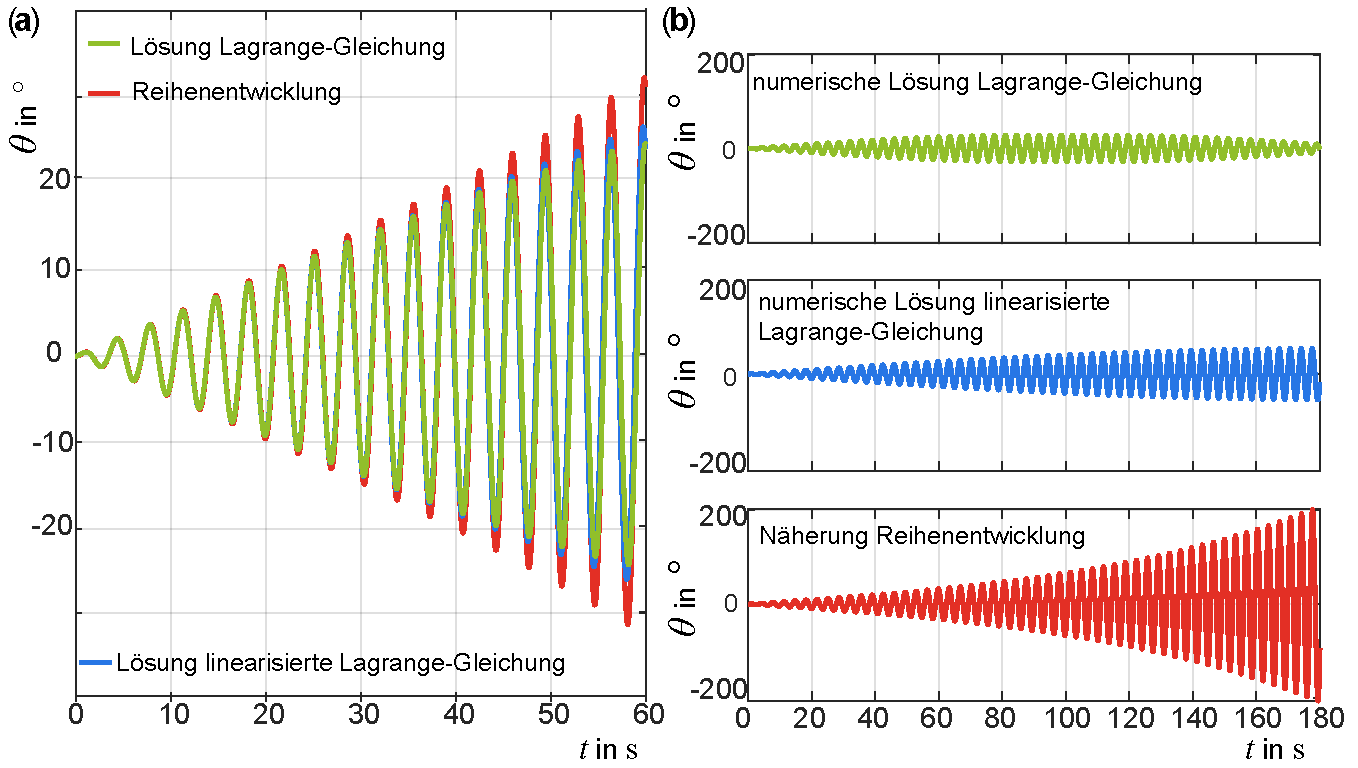
\includegraphics[width=\textwidth]{Schaukel05.pdf}
\caption[Dynamik einer Schaukel als getriebener Oszillator.]{L�sung der Bewegungsgleichung f�r das Modell einer Schaukel als ein getriebener Oszillator f�r \fa Anfangsphase (Kind) und \b l�ngere Zeiten (Erwachsener). Parameter entsprechend \figref{bew_schaukel01} und Tab. \ref{tab:bew_schaukel01}.} 
\label{abb:bew_schaukel05}
\end{figure}

In \probref{bew_schaukelII} schauen wir uns noch die Situation einer im Stehen schaukelnden Person an (siehe auch \cite{Case1996}).
Das Problem kann v�llig analog wie im Fall der sitzenden schaukelnden Person behandelt werden und ergibt als L�sung wieder einen getriebenen Oszillator mit parametrischen Elementen. Noch einen Hinweis zum Schluss: Falls man mal eine Person auf einer Schaukel sieht, die versucht, die Schaukel durch reine parametrische Oszillation, d.h. durch Heben und Senken des K�rpers anzuregen, dann kann man ziemlich sicher sein, dass es sich um einen (theoretischen) Physiker handelt. 


\subsection{Fallende starre K�rper und die rutschende Leiter} \label{kap:bew_fallendeKoerper}

Die einfachen Experimente von fallenden St�ben (und anderen K�rpern wie \zb einem Smartphone)
oder das einer rutschenden Leiter erlauben einige sch�ne Anwendungen
der Physik des starren K�rpers und dar�ber hinaus auch unter Nutzung
von Videokamera und Beschleunigungssensor des Smartphones die einfache
experimentelle �berpr�fung der theoretischen Betrachtungen
und numerischen Rechnungen \cite{Cross2006,Oliveira2016,Kaps2020}.
Sie ergeben dar�ber hinaus, so einfach sie auf den ersten Blick erscheinen, tiefe Einblicke in das Zusammenspiel von Drehmomenten, Reibungskr�ften und tempor�ren Zwangsbedingungen. 


\subsubsection{Fall eines Stabes} \label{kap:bew_fallenderStab}

	Wir beginnen mit dem Umfallen eines urspr�nglich fast senkrecht stehenden Stabes
        ($\theta_0$ betrage einige Grade).
        Wir betrachten dazu \figref{bew_fallingrod01}.
        Der Stab befinde sich auf einer Oberfl�che mit dem Reibungskoeffizienten $\mu$.
        Es wirken neben der Gewichtskraft am Fu�punkt des Stabes
        die Horizontalkraft $F_\text{H}$ und dazu senkrecht die Normalkraft $F_\text{N}$.
        Offensichtlich wird die Reibung einen gro�en Einfluss auf die Bewegung haben.
        Bei einem reibungsfreien Tisch w�rde der Stab einfach wegrutschen
        und der Schwerpunkt sich senkrecht nach unten bewegen.

\begin{figure}
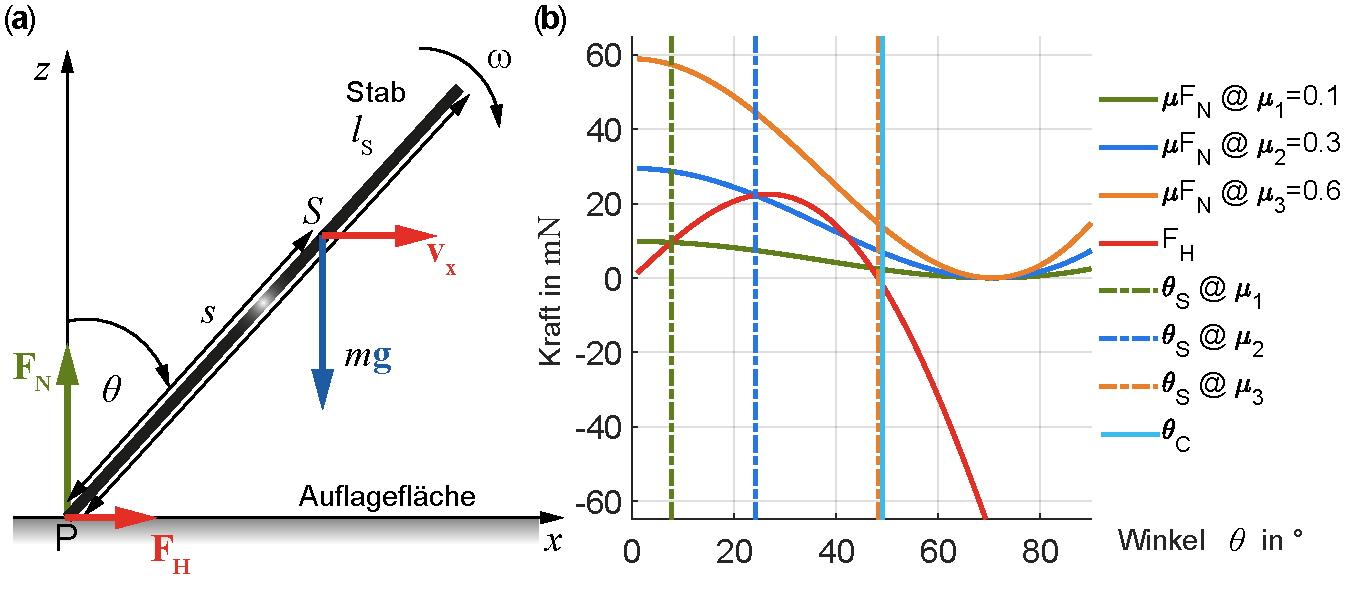
\includegraphics[width=\textwidth]{FallingRod01.pdf}%
\caption[Geometrie und Kr�fte beim umfallenden Stab.]{Geometrie und Kr�fte beim umfallenden Stab. \fa Geometrie und \fb wirkende Kr�fte beim umfallenden Stab. Wenn $F_\text{H} = \mu\,F_\text{N}$ wird, beginnt der Stab bei $\theta_\text{S}$ (f�r $\mu_1$ und $\mu_2$) zu rutschen (gleiten), davor ist der Fu�punkt auf der Unterlage feststehend. F�r das  gr��ere $\mu_3$ beginnt die Gleitphase des Stabes bei $\theta_\text{C}$.}
\label{abb:bew_fallingrod01}
\end{figure}

    Ferner sei $m$ die Masse des Stabes, $\dot{x} = v_\text{x}$ und $\dot{z} = v_\text{z}$ dessen Schwerpunktsgeschwindigkeit in $x$- \bzw $z$-Richtung, $s$ der Abstand des Schwerpunktes vom Fu�punkt am Boden und $J_\text{S}$ das Tr�gheitsmoment bezogen auf den Schwerpunkt.
    Dann gelten die folgenden Bewegungsgleichungen  f�r die generalisierten Koordinaten $x$, $y$, $\theta$:
    \begin{align}
        F_\text{R} &= m\,\ddot{x}\,, \label{eq:bew_fallingrod01a}\\
        F_\text{N} &= m\,\lk \ddot{z} + g \rk\,,\label{eq:bew_fallingrod01b}\\
        M_\text{P} &= F_\text{N}\,s\,\sin\theta - F_\text{H}\,s\,\cos\theta = J_\text{S}\,\ddot{\theta}\,. \label{eq:bew_fallingrod01c}
    \end{align}
Als Anfangsbedingung wollen wir $\dot{z}\lk 0 \rk = v_\text{z}\lk 0\rk = 0$ und $\dot{x}\lk 0 \rk = v_\text{x}\lk 0\rk = 0$,\\ $\dot{\theta}\lk 0\rk = \dot{\theta}_0 = 0$, sowie $\theta\lk 0\rk = \theta_0 > 0$ annehmen.\\
Wir beschreiben zun�chst den Bewegungsablauf genauer, eine Beobachtung desselben ist mit einer Hochgeschwindigkeitsvideoaufnahme mit dem Smartphone leicht zu realisieren:
\begin{enumerate}
    \item Zu Beginn wird der Stab einfach umfallen, das hei�t, $\theta\,, \,\dot{\theta}$ werden mit fortlaufender Zeit gr��er und das untere Fu�ende bleibt ortsfest, solange $F_\text{H} < \mu\,F_\text{N}$. \\
	Wir beschreiben diesen Teil der Bewegung als reine Rotation um den Punkt $P$,
        sodass $\dot{x} = s\,\omega\,\cos\theta$ und $\dot{z} = -s\,\omega\sin\theta$
        und erhalten mit $\dot{\theta} = \omega$ und \eqref{eq:bew_fallingrod01b}
    \begin{align}
      F_\text{H} &= m\,s\,\lk \cos\theta\,\dot{\omega} - \sin\theta\,\omega^2\rk \text{und} \label{eq:bew_fallingrod02}\\
      F_\text{N} &= m\,g -m\,s\,\lk \sin\theta\,\dot{\omega} + \cos\theta\,\omega^2\rk \,. \label{eq:bew_fallingrod03}
    \end{align}
	Wir setzen \eqref{eq:bew_fallingrod02} und \eqref{eq:bew_fallingrod03} in \eqref{eq:bew_fallingrod01c} ein und erhalten mit
	\begin{align}
		\dot{\omega} = \ddot{\theta} = {\omega_0}^2\,\sin\theta ~~\text{und}~~ {\omega_0}^2 = \lk {m\,g\,s}\rk/J_\text{P}  \label{eq:bew_fallingrod04}
	\end{align}
	eine bemerkenswert einfache Gleichung f�r $\theta$ mit $J_\text{P} = J_\text{S} + m\,s^2$ als Tr�gheitsmoment bez�glich des Fu�punktes.
        Letzteres gilt f�r homogene St�be $J_\text{P} = m\,l_\text{S}{}^2/3$ mit $l_\text{S}=2s$.
        Wir weisen nochmals darauf hin, dass \eqref{eq:bew_fallingrod04} nur gilt,
        solange der Punkt $P$ fest bleibt.
        Dann kann man \eqref{eq:bew_fallingrod04} integrieren und erh�lt,
        wie man durch Differenzieren leicht nachrechnet,
    \begin{align}
        \omega^2 = 2\,{\omega_0}^2\,\lk\cos\theta_0-\cos\theta\rk \,,\label{eq:bew_fallingrod05}
    \end{align}
sodass sich f�r die Kr�fte $F_\text{H}, \, F_\text{N}$ als Funktion des Winkels $\theta$ mit \eqref{eq:bew_fallingrod02} und \eqref{eq:bew_fallingrod03} ergibt: 
    \begin{align}
    \begin{split}
        F_\text{H} &= m\,s\,{\omega_0}^2\,\sin\theta\,\lk 3\cos\theta-2\cos\theta_0\rk \,, \\
        F_\text{N} &= m\,g - m\,s\,{\omega_0}^2\,\lk 1+2\cos\theta\,\cos\theta_0 - 3\cos^2\theta\rk \,. \label{eq:bew_fallingrod06}
    \end{split}
    \end{align}
		Die Kr�fte $F_\text{H}, \, F_\text{N}$ sind in \figref{bew_fallingrod01}b (siehe auch \mscr{} \mlbewref{FallenderStab01.m}) dargestellt.
                Man erkennt aus \eqref{eq:bew_fallingrod06} und der Abbildung, dass die Horizontalkraft $F_\text{H}$ sich ab einem bestimmten Winkel verringert und dann das Vorzeichen wechselt.%
                \footnote{Physikalisch kann man das als Ergebnis der Horizontalkomponente der wirkenden Zentripetalkraft des drehenden Stabes verstehen.} 
    \item Bei einem bestimmten Winkel $\theta_\text{S}$
      abh�ngig von der Oberfl�chenreibung $\mu$ des Tisches
      wird der untere Fu�punkt des Stabes ins Rutschen/Gleiten kommen,
      da dann $F_\text{H}(\theta_\text{S}) = \mu\, F_\text{N}(\theta_\text{S})$ gilt.
      Mit \eqref{eq:bew_fallingrod06} berechnet sich der Winkel $\theta_\text{S}$ aus
      \footnote{Eigentlich m�sste man bei der Behandlung der Reibung
      zwischen Haftreibung $\mu_\text{H}$ und Gleitreibung $\mu_\text{G}$ unterscheiden.
      Wir empfehlen dem Leser, das f�r die numerische Berechnung zu tun,
      in der einfach eine entsprechende Fallunterscheidung programmiert werden kann.}
    \begin{align}
	\begin{split}
        \mu &= \frac{m\,s\,{\omega_0}^2\,\sin\theta_\text{S}\,\lk 3\cos\theta_\text{S}-2\cos\theta_0\rk }{m\,g - m\,s\,{\omega_0}^2\,\lk 1+2\theta_\text{S}\,\cos\theta_0 - 3\cos^2\theta_\text{S}\rk }\, \\
				&\text{\bzw f�r einen homogenen Stab} \\
				\mu &= \frac{9\sin\theta_\text{S}\,\cos\theta-6\cos\theta_0\,\sin\theta_\text{S}}{1+9\cos^2\theta_\text{S}-6\cos\theta_0\,\cos\theta_\text{S}} \,.
				\label{eq:bew_fallingrod07}
	\end{split}
    \end{align}
	In \figref{bew_fallingrod01}b sind f�r die zwei Reibungskoeffzienten
        $\mu_1$ und $\mu_2$ die entsprechenden Winkel $\theta_\text{S}(\mu)$
        eingezeichnet.
        Man erkennt sehr sch�n, dass dort tats�chlich
        $F_\text{H}(\theta_\text{S}) = \mu\, F_\text{N}(\theta_\text{S})$ gilt.
	\item In \figref{bew_fallingrod01}b ebenfalls eingezeichnet
          ist der kritische Winkel $\theta_\text{C}$,
          bei welchem die Horizontalkraft $F_\text{H} = 0$ ist.
          Bei diesem Winkel beginnt unabh�ngig vom Reibungskoeffizienten $\mu$
          der Stab am Fu�punkt auf jeden Fall zu gleiten.
          Der Winkel $\theta_\text{C}$ berechnet sich f�r einen homogenen Stab zu
    \begin{align}
	\theta_\text{C} =\arccos\lk \frac{2}{3} \cos\theta_0 \rk \,. 	\label{eq:bew_fallingrod08}
    \end{align}
	\item Es gibt also zwei m�gliche Einsetzpunkte des Gleitens:
          $\theta_\text{S}$ und $\theta_\text{C}$.
          Beim Einsetzen bei $\theta_\text{S}$ wird das untere Ende des Stabes
          zu kleineren $x$-Werten rutschen, beim Einsetzen bei $\theta_\text{C}$ umgekehrt. 
\end{enumerate}
Wir haben damit nun alle Informationen, um die Bewegung analytisch zu beschreiben
und auch numerisch zu berechnen.
Wir unterteilen dazu die Bewegung in zwei Phasen,
die einfache Rotation um den Punkt $P$ und die gekoppelte Rotation
mit der horizontalen Bewegung des Fu�punktes.
Wir betrachten zun�chst die reine Rotation um den Punkt $P$.
Hier k�nnen wir einfach die Bewegungsgleichung \eqref{eq:bew_fallingrod04}
numerisch bis $\theta_\text{S}$ \bzw $\theta_\text{C}$ integrieren.
Etwas schwieriger ist die Phase 2.
F�r diese Phase muss man in \eqref{eq:bew_fallingrod02}
$F_\text{R} = \mu\,F_\text{N}$ setzen und erh�lt daraus
mit \eqref{eq:bew_fallingrod01c} und \eqref{eq:bew_fallingrod03}
die folgende Bewegungsgleichung f�r $\ddot{\theta}$: 
    \begin{align}
	\begin{split}
        \ddot{\theta} &= \frac{m\,s\,\lk g-s\,\dot{\theta}^2\,\cos\theta\rk\lk\sin\theta-\mu\,\cos\theta\rk}{J_\text{S} + m\,H^2\,\sin\theta\,\lk \sin\theta-\mu\cos\theta\rk} \\
				&\text{\bzw f�r einen homogenen Stab} \\
	\ddot{\theta} &= \frac{\frac{g}{s} - {\dot{\theta}}^2\,\cos\theta}{\sin\theta + C(\theta)} ~~~\text{mit} ~~~ C(\theta) = \lk 3 \sin\theta - 3 \mu \cos\theta \rk^{-1}\,. \label{eq:bew_fallingrod08a}
	\end{split}
    \end{align}
Man beachte, dass je nach der Art des Einsetzens des Gleitens,
\dh je nachdem, ob $F_\text{H}$ zum Zeitpunkt des Einsetzens des Rutschens
bereits das Vorzeichen gewechselt hat, $\mu>0$ (f�r $\theta_\text{S}$)
\bzw $\mu<0$ (f�r $\theta_\text{C}$) gesetzt werden muss.
In der numerischen Rechnung im \mscr{} \mlbewref{FallenderStab02.m}
wird das entsprechend ber�cksichtigt.
Zus�tzlich muss noch die Bewegung des Fu�punktes $x_\text{P}$ berechnet werden.
F�r den homogenen Stab ergibt sich aus den Bewegungsgleichungen
\eqref{eq:bew_fallingrod01a}--\eqref{eq:bew_fallingrod01c} \cite{Oliveira2016}:
    \begin{align}
        \ddot{x}_\text{P} &= s \, \dot{\theta}^2 \sin\theta - s\, \ddot{\theta} \lk \cos\theta - \mu\, C(\theta) \rk\,. \label{eq:bew_fallingrod08b}
    \end{align}

\begin{figure}
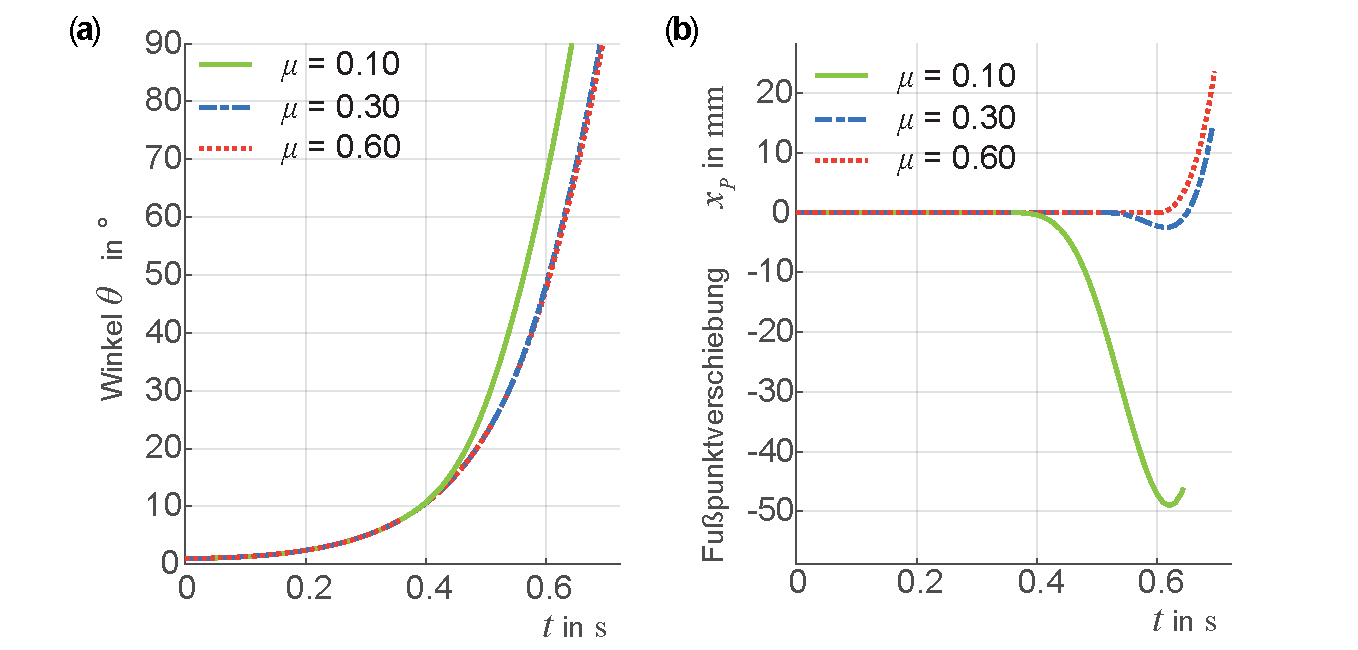
\includegraphics[width=\textwidth]{FallingRod02.pdf}%
\caption[Dynamik eines umfallenden Stabes.]{Dynamik eines umfallenden Stabes. \fa Dargestellt ist die zeitliche Entwicklung des Winkels $\theta(t)$ f�r verschiedene Reibungen. \fb $x$-Position des Stabendes als Funktion der Zeit f�r verschiedene Reibungskoeffizienten.} \label{abb:bew_fallingrod02}
\end{figure}

In \figref{bew_fallingrod02}a haben wir den Fallwinkel $\theta$
als Funktion der Zeit f�r verschiedene Reibungskoeffizienten berechnet.
Man erkennt eine relativ geringe Abh�ngigkeit der Fallzeit vom Reibungskoeffizienten.
\figref{bew_fallingrod02}b zeigt den Fu�punkt $x_\text{P}$ des Stabes
als Funktion der Zeit, wiederum f�r verschiedene Reibungskoeffizienten.
Man erkennt, dass f�r eine rauere Oberfl�che (ein gr��eres $\mu$)
das Stabende sich in Neigungsrichtung ($x >0$) bewegt,
w�hrend f�r eine glattere Oberfl�che, wie nicht anders zu erwarten war,
das Stabende sich (zun�chst) in entgegengesetzte Richtung bewegt, also wegrutscht.
Dieses interessante Verhalten des Stabes, insbesondere auch
das R�ckw�rts- und anschlie�ende Vorw�rtsgleiten bei geringen $\mu$,
kann durch das Zusammenspiel der Horizontalkomponente der Linearbeschleunigung
und der Zentripetalkraft ($\propto \dot{\theta}$)
des drehenden Stabes verstanden werden.
Dem Leser wird empfohlen, mit dem 
\mscr{} \mlbewref{FallenderStab02.m} auch die $\theta_0$-Abh�ngigkeit
und die Wirkung inhomogener Massenverteilungen zu studieren.\\
Zum Schluss sei noch im Zusammenhang mit dem behandelten Problem
auf eine interessante Frage verwiesen:
Kann das Fu�ende des Stabes \anf{abheben}, \dh kann zu irgendeinem Zeitpunkt
w�hrend des Fallens $z_\text{P} > 0$ gelten?%
\footnote{Wir �berlassen dem Leser die (numerische) �berpr�fung.}
Diese Frage ist �brigens eng verwandt mit der Frage
nach der maximalen Gehgeschwindigkeit des Menschen:
Bis zu welcher Bewegungsgeschwindigkeit $v$ bleibt der K�rper
mit mindestens einem Fu� auf dem Boden?
Da der Schwerpunkt des K�rpers eines Menschen ($s\approx \SI{1}{\metre}$)
um den Fu�auflagepunkt \anf{rotiert}, gilt f�r die Normalkraft
    \[F_\text{N} \approx m\,g - m\,v^2/s\,,\]
und damit $F_\text{N}>0$ bleibt, darf die Geschwindigkeit
nicht gr��er als $v_\text{max} =\sqrt{g\,s} \approx \SI{3}{\metre\per\s}$ werden,
was gut mit der Erfahrung �bereinstimmt.
Beim sportlichen Gehen erreichen die schnellsten M�nner
Geschwindigkeiten von $v_\text{max} =\sqrt{g\,s} \approx 4.5 \text{ bis } \SI{5}{\metre\per\s}$,
was nur durch eine spezielle Geher-Technik erreicht wird.

\subsubsection{Vergleich umfallender St�be mit verschiedenen Masseverteilungen}

Bevor wir uns dem verwandten Problem der rutschenden Leiter zuwenden,
wollen wir uns noch einen \glqq Wettbewerb\grqq{} �berlegen
und 3 umfallende St�be der L�nge $l_\text{S}$ mit unterschiedlicher Masseverteilung vergleichen \cite{Shan2020}.
\begin{enumerate}
    \item [a)] homogener Stab der Gesamtmasse $m+m_\text{T}$
    \item [b)] homogener Stab der Masse $m$ mit Gewicht $m_\text{T}$ am Ende des Stabes
    \item [c)] homogener Stab der Masse $m$ mit 2 Gewichten $m_\text{T}/2$ an den Positionen $l_\text{S}/3$ und $2 l_\text{S}/3$
\end{enumerate}
Welcher Stab erreicht als erster die Horizontale? Wir wollen uns die Rechnung etwas vereinfachen und nehmen das Fu�ende als festgehalten an,
was $\mu \rightarrow\infty$ entspricht. Bei festem Drehpunkt k�nnen wir die Bewegungsgleichungen entsprechend \eqref{eq:bew_fallingrod04} aufschreiben und folgende Tr�gheitsmomente und Schwerpunktlagen berechnen (dabei sei $m_\text{T}/m = \gamma = 5$ angenommen):
    \begin{align}
        J_\text{a} &= \frac{1}{3}\,\lk m+m_\text{T}\rk\,l_\text{S}^2 = 2m\,l_\text{S}^2
        &r_\text{s,a} &= \frac{l_\text{S}}{2} \,,\notag\\
        J_\text{b} &=\frac{1}{3}\,m\,l_\text{S}^2 + m_\text{T}\,l_\text{S}^2 = \frac{16}{3}\,m\,l_\text{S}^2
        &r_\text{s,b} &= \frac{11}{12}\,l_\text{S}\,,
    \label{eq:bew_fallingrod09}
        \\
        J_\text{c} &=\frac{1}{3}\,m\,l_\text{S}^2 + \frac{m_\text{T}}{2}\,\lek\frac{l_\text{S}^2}{9} + \frac{4L^2}{9}\rek = \frac{11}{18}\,m\,l_\text{S}^2
        &r_\text{s,c} &=  \frac{l_\text{S}}{2} = r_\text{s,a}\,. \notag
    \end{align}
Die Winkelbeschleunigungen $\ddot{\theta}_\text{i}$ ergeben sich mit den Drehmomenten $M_\text{D,i}$ zu
    \begin{align}
      \ddot{\theta}_i = \frac{M_{\text{D},i}}{J_i} = \frac{\lk m+m_\text{T}\rk\,g\,r_{\text{s},i}\,\sin\theta}{J_i} ~~~~~i = \text{a,b,c} \label{eq:bew_fallingrod10}
    \end{align}
\bzw im einzelnen Fall durch
\begin{align*}
			\ddot{\theta}_\text{a} &= \frac{3}{2}\,g\,\sin\theta / l_\text{S}\,,~
			~~~\ddot{\theta}_\text{b} = \frac{33}{32}\,g\,\sin\theta / l_\text{S}\,,~
			~~~\ddot{\theta}_\text{c} = \frac{54}{11}\,g\,\sin\theta / l_\text{S}\,.
\end{align*}
\begin{figure}
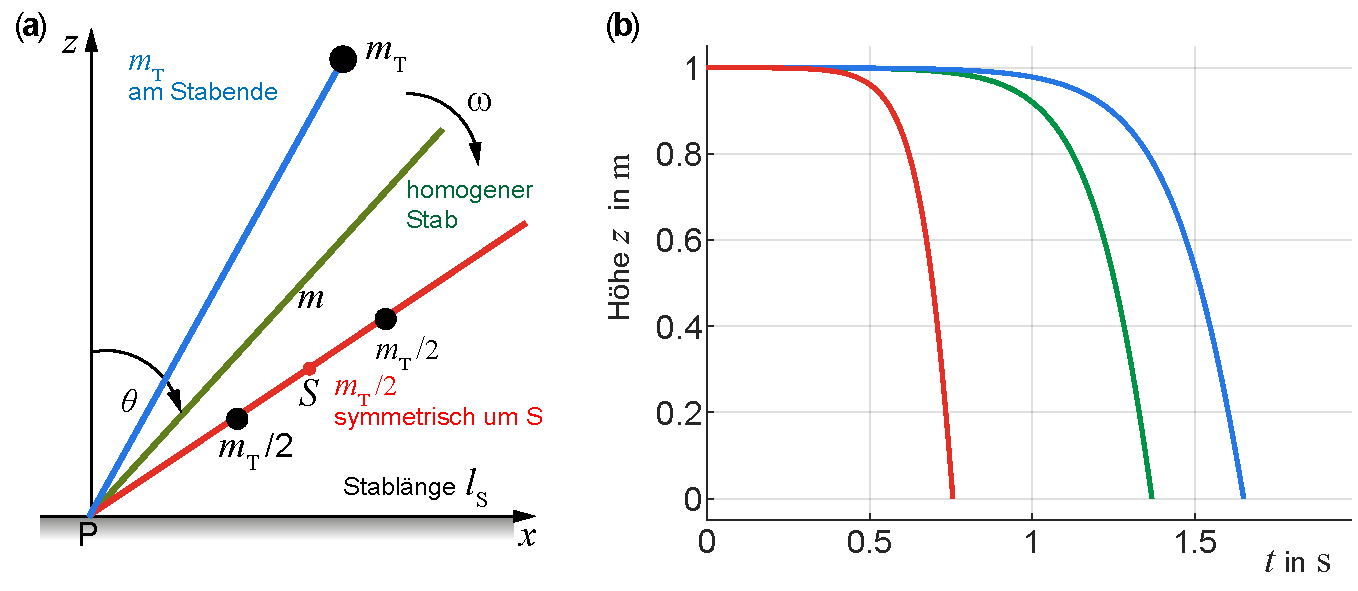
\includegraphics[width=\textwidth]{FallingRod03.pdf}%
\caption[Dynamik umfallender St�be verschiedener Massenverteilungen.]{Dynamik umfallender St�be verschiedener Massenverteilungen.} \label{abb:bew_fallingrod03}
\end{figure}
Die Integration der Bewegungsgleichung ist in \figref{bew_fallingrod03} dargestellt.
Wie man sieht, f�llt der Stab c am schnellsten fallende Stab.
Die unterschiedlichen Fallzeiten haben ihre Ursache darin,
dass in \eqref{eq:bew_fallingrod09} und \eqref{eq:bew_fallingrod10}
sowohl das Tr�gheitsmoment als auch das wirkende Drehmoment
von der Massenverteilung entlang des Stabes abh�ngig sind. \\

\subsubsection{Umfallende Leiter} \label{kap:bew_fallendeLeiter}

\begin{figure}
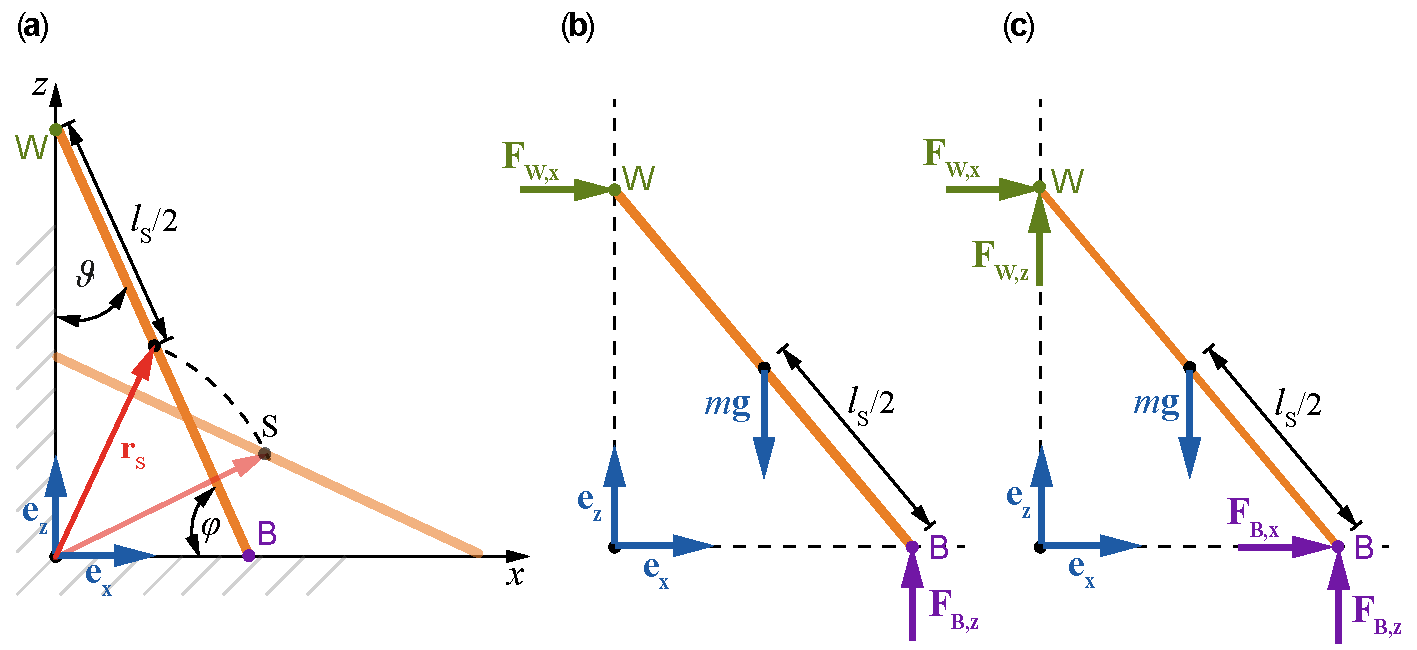
\includegraphics[width=\textwidth]{Ladder01.pdf}%
\caption[Geometrie und Kr�fte der umfallenden Leiter.]{Geometrie und Kr�fte der umfallenden Leiter. \fa Geometrie, \fb Normalkr�fte und \fc Normal- und Reibungskr�fte.} \label{abb:bew_ladder01}
\end{figure}

Eines der scheinbar einfachen Probleme der Mechanik ist das der \anf{umfallenden} \bzw \anf{wegrutschenden} Leiter.
So einfach es auf den ersten Blick erscheint,
so �berraschend sind doch die dabei zu ber�cksichtigenden physikalischen Effekte,
sodass es bis heute \zt einander widersprechende Ver�ffentlichungen
zu diesem Problem gibt, siehe dazu \cite{Oliveira2015, Glane2019, Ghorashi2019} und dort angegebene Referenzen.

Wir betrachten \figref{bew_ladder01}\,a, nehmen die Leiter als homogen an und stellen zun�chst eine einfache energetische Betrachtung an.

\subparagraph{Energiebetrachtung f�r die fallende Leiter}~

Aus der Abbildung sehen wir, dass der Vektor $\vec r$ vom Ursprung zum Schwerpunkt S
beim Rutschen der Leiter zun�chst eine Kreisbahn beschreibt.
Interessant ist der Punkt \bzw die Richtung von $\vec r$, bei dem die Leiter den Kontakt
zur Wand am Punkt B oder W verliert.
Dies wird bei einem Winkel $\vartheta_S=90\degree - \varphi_S$ passieren, bei dem die $x$-Komponente
der Schwerpunktgeschwindigkeit abnimmt,
\dh die Beschleunigung und damit die Normalkraft am Punkt W negativ werden m�sste.
Das ist aber physikalisch unm�glich, sodass dies der Punkt ist,
ab dem die Leiter sich von der Wand l�st, also richtig \anf{wegrutscht}.

Aus der Energieerhaltung folgt f�r die Schwerpunktskoordinaten ausgedr�ckt �ber den Winkel $\vartheta$
\begin{align}
 \Delta U &= T_{\text{Trans}} + T_{\text{Rot}}\,=\, m\,g\,r(1-\cos\vartheta) = \frac m2\lk\dot x^2+\dot z^2\rk + \frac J2 \dot\vartheta^2\notag\\
  &=\frac m2r^2\dot\vartheta^2 + \frac J2\dot\vartheta^2 = \frac12\lk mr^2+J\rk\dot\vartheta^2\,.
  \label{eq:bew_ladder01}
\end{align}

F�r die homogene Masseverteilung gilt $J=\frac1{12}m l_\text{S}{}^2=\frac13mr^2$.

Wir l�sen \eqref{eq:bew_ladder01} nach $v=r\vartheta$ und erhalten f�r die Horizontalkomponente der Schwerpunktsgeschwindigkeit 
\begin{align}
  v_x &= v\, \sin(90\degree -\vartheta) = \sqrt{\frac{3gr(1-\cos\vartheta)}2}\,\cos\vartheta
	    = \sqrt{\frac{3gr}2}\sqrt{(1-u)u^2}\,.\label{eq:bew_ladder02}
\end{align}

Wir suchen das Maximum von $v_x$
(da ab dort eine Verringerung der Horizontalgeschwindigkeit einsetzen w�rde)
und erhalten
\begin{equation}
  \cos\vartheta_S = \frac23\quad\rightarrow\quad\vartheta_S\approx\SI{48.2}{\degree}\,.
  \label{eq:bew_ladder03}
\end{equation}

Man kann nun noch fragen, bei welchem Winkel $\vartheta_M$ die Leiter am Punkt W
die maximale Normalkraft der Wand erf�hrt, \dh am sichersten an der Wand steht.

Wir bilden
\begin{align}
  F_{N,W} &\propto \frac{\D}{\D\vartheta}v_x\cdot\frac{\D\vartheta}{\D t}\propto\lk\frac12\frac{\cos\vartheta\sin\vartheta}{\sqrt{1-\cos\vartheta}}
  -\sqrt{1-\cos\vartheta}\sin\vartheta\rk\dot\vartheta\notag\\
  &=\dot\vartheta\sin\vartheta\lek\frac{\cos\vartheta-1+2\cos\vartheta}{\sqrt{1-\cos\vartheta}}\rek \propto\sin\vartheta(3\cos\vartheta-2)\cdot\dot\vartheta\,.
  \label{eq:bew_ladder04}
\end{align}
Die Maximalbedingung ergibt
\begin{align*}
  \frac{\partial F_{N,W}}{\partial\vartheta}=0
  &=\cos\vartheta(3\cos\vartheta-2) - 3\sin\vartheta\,\sin\vartheta \\
  %&=3\cos^2\vartheta -2\cos\vartheta - 3\sin^2\vartheta\\
  %&=3\cos^2\vartheta - 2\cos\vartheta - 3 + 3 \cos^2\vartheta\\
  &=6\cos^2\vartheta - 2\cos\vartheta - 3
\end{align*}
und mit $u=\cos\vartheta$
\begin{align}
  u^2-\frac13u-\frac12 &= 0\,~~\rightarrow~~ f_{1,2} = \frac16\pm\sqrt{\frac1{36}+\frac{18}{36}}= \frac16\pm\frac{\sqrt{19}}6\,,
  \label{eq:bew_ladder05}
\end{align}
wir erhalten also $\cos\vartheta_M = \frac16(1+\sqrt{19})$ und mithin $\vartheta_M\approx\SI{26.7}{\degree}$.
Man tut also gut daran, die Leiter etwas steiler als
$\varphi = \SI{90}{\degree}-\vartheta = \SI{60}{\degree}$ zu stellen.

\subparagraph{Dynamische Betrachtung}

Nach diesen eher grunds�tzlichen �berlegungen wollen wir uns nun der Dynamik zuwenden und benutzen dabei vorteilhafterweise den Winkel $\varphi$ als generalisierte Koordinate.

Wir betrachten \figref{bew_ladder01}, wo wir im Fall b)
die Leiter ohne Reibungseinfluss der W�nde betrachten wollen und im Fall c)
mit den Reibungskr�ften von Wand und Boden.
Aus der Zwangsbedingung, dass die Leiter bis zum Abl�sen
in Kontakt zu Wand und Boden ist,
k�nnen wir folgende kinematische Bedingungen als Funktion von $\varphi(t)$ aufschreiben:
\begin{align}
  %\text{Auflagepunkte B,W:}  \notag\\
  \vec x_n &= x_B\,\vec e_x = l_\text{S}\,\cos\varphi\vec e_x\,,~~ \vec z_W = z_W\,t\vec e_z = l_\text{S}\,\sin\varphi\vec e_z\notag\\
  %\text{Schwerpunkt S:} \notag\\ 
  \vec x_S &= \frac{ l_\text{S}}{2}\cos\varphi\vec e_x + \frac{ l_\text{S}}{2} \sin\varphi\vec e_z\,,~~ \dot{\vec x}_S = \frac{ l_\text{S}}{2}\dot\varphi\lk\sin\varphi\vec e_x+\cos\varphi\vec e_z\rk
  \notag\\
  \ddot{\vec x}_S &= \frac{ l_\text{S}}{2}\lek\lk-\sin\varphi\cdot\ddot\varphi-\cos\varphi\dot\varphi^2\rk\vec e_x
  +\lk\cos\varphi\ddot\varphi-\sin\varphi\dot\varphi^2\rk\vec e_z\rek\,.
  \label{eq:bew_ladder06}
\end{align}

Wir schreiben nun die Kr�fte und Drehmomente gem�� \figref{bew_ladder01}b auf:
\begin{align}
\begin{split}
  m\,\ddot{\vec x}_S &= F_{W,x}\,\vec e_x + \lk F_{B,z} - mg\rk\,\vec e_z\,, \\
  J_S\,\ddot\varphi &= -(x_B-x_S)\,F_{B,z} - (z_W-z_S)\,F_{W,x}\,.
\end{split}
  \label{eq:bew_ladder07}
\end{align}

Das Minuszeichen resultiert aus der Tatsache, dass die rutschende Leiter
sich gegen den Uhrzeigersinn \anf{dreht}. Setzen wir \eqref{eq:bew_ladder06} in \eqref{eq:bew_ladder07} ein,
erhalten wir durch Elimination der Wandkr�fte die Bewegungsgleichung f�r $\varphi(t)$
f�r $J_S=\frac1{12}m l_\text{S}{}^2$:
\begin{equation}
  \ddot\varphi(t) = -\frac32\frac{g}{l_\text{S}}\cos\varphi(t)\,.
  \label{eq:bew_ladder08}
\end{equation}

Die Normalkr�fte an Wand und Boden als Funktion des Winkels lauten
\begin{align*}
  F_{B,z} &= -\frac{m l_\text{S}}2\lk\frac{3g}{2 l_\text{S}}\cos^2\varphi+\sin\varphi\,\dot\varphi^2\rk \,+\,m\,g~~~\text{ und}\\
  F_{W,x} &= +\frac{m l_\text{S}}2\cos\varphi\lk\frac{3g}{2 l_\text{S}}\sin\varphi-\dot\varphi^2\rk\,.
\end{align*}

\begin{figure}
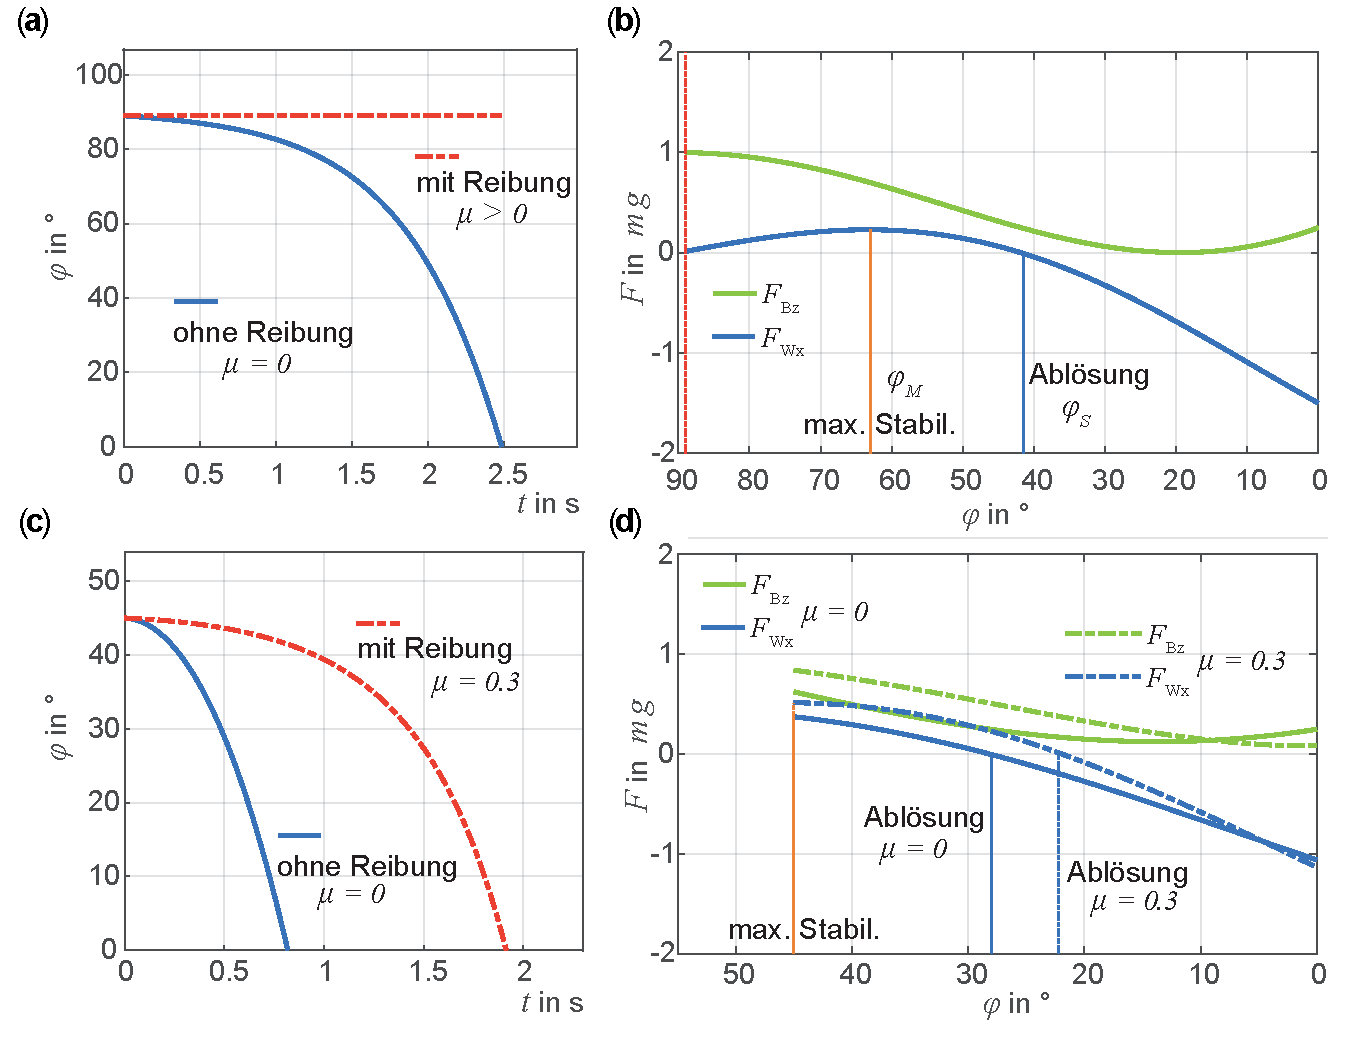
\includegraphics[width=\textwidth]{Ladder02.pdf}
\caption[Dynamik der umfallenden Leiter mit und ohne Reibung.]{Dynamik der umfallenden Leiter mit und ohne Reibung.
\fa Dynamik mit $\vartheta(0) \approx 0 \cong \varphi(0) \approx 90\degree$.
Bei $\mu >0$ rutscht die Leiter nicht weg.
\fb Normalkr�fte an Wand und Boden bei $\vartheta(0) = 0 \equiv \varphi(0) \approx 90\degree$.
Die Abl�sung der Leiter erfolgt im reibungsfreien Fall bei $\varphi_S\approx 42\degree$  \bzw $\vartheta_S\approx 48\degree$,
die maximale Stabilit�t hat die Leiter bei $\varphi_M\approx 63\degree$ \bzw $\vartheta_M\approx 27\degree$.
\fc Dynamik mit Startwinkel der Leiter bei $\varphi(0) = \vartheta(0) = 45\degree$.
Hier rutscht die Leiter auch bei $\mu = 0.3$ weg, aber entsprechend langsamer als im reibungsfreien Fall.
\fd Normalkr�fte an Wand und Boden bei $\varphi(0) \approx 45\degree$.
Die Abl�sung der Leiter im reibungsfreien Fall erfolgt bei $\varphi_S\approx 28\degree$, bei einem Reibungskoeffizienten von $\mu = 0.3$ erst bei $\varphi_S\approx 22.5\degree$
(Siehe \mscr{} \mlbewref{FallendeLeiter.m}).} \label{abb:bew_ladder02}
\end{figure}

In \figref{bew_ladder02} haben wir die zeitliche Entwicklung von $\varphi(t)$
und die Kr�fte $F_{B,z},\, F_{W,x}$ dargestellt. Die Rechnungen best�tigen unser �ber den Energieerhaltungssatz erhaltenes Ergebnis
\eqref{eq:bew_ladder05}.

Wir k�nnen uns jetzt noch fragen, welchen Einfluss die Reibung an Wand und Boden
auf die Dynamik der fallenden Leiter hat.
Dazu m�ssen wir \eqref{eq:bew_ladder07} um die Reibungskr�fte erweitern und erhalten
\begin{align}
\begin{split}
  m\,\ddot{\vec{x}}_S &= (F_{B,x}+F_{W,x})\,\vec e_x + (F_{B,z}+F_{W,z}-mg)\,\vec e_z\,, \\
  J_S\,\ddot\varphi &= -(z_B-z_S)\,F_{B,x} + (x_B-x_S)\,F_{B,z} \\
  &= -(z_W-z_S)\,F_{W,x} + (x_W-x_S)\,F_{W,z}\,.
\end{split}
  \label{eq:bew_ladder09}
\end{align}
Hierin sind jetzt $F_{B,x}$ und $F_{W,z}$
die Komponenten der Reibungskr�fte, die wir als Gleitreibungskr�fte annehmen k�nnen,
sodass wir mit der Vereinfachung $\mu_W = \mu_B = \mu$ schreiben k�nnen:
\begin{align}
\begin{split}
  F_{B,x} &= -\sgn(\vec v_B\cdot\vec e_x)\,\mu\,|F_{B,z}| = \sgn(\dot\varphi)\,\mu\,|F_{B,z}| \; , \\
  F_{W,z} &= -\sgn(\vec v_W\cdot\vec e_z)\,\mu\,|F_{W,x}| = -\sgn(\dot\varphi)\,\mu\,|F_{W,x}|\;.
\end{split}
 \label{eq:bew_ladder10}
\end{align}

Die Reibungskr�fte $F_{B,x}$ \bzw $F_{W,z}$ an Boden und Wand sind hierbei �ber die 
an der Wand \bzw am Boden wirkenden Normalkr�fte definiert.
Wegen der Richtungsabh�ngigkeit haben wir vorteilhaft die $\sgn$-Funktion%
\footnote{In \matlab{} und auch vielen B�chern wird die $\sgn$-Funktion mit $\mathrm{sign}$ bezeichnet.} benutzt
\cite{Glane2019}:
\begin{equation}
  \sgn(x) = \begin{cases}
    1 & x > 0\\
    0 & x = 0\\
    -1 & x < 0
  \end{cases}\,.
  \label{eq:bew_ladder11}
\end{equation}
Wir eliminieren nun mit \eqref{eq:bew_ladder11}, \eqref{eq:bew_ladder10} und \eqref{eq:bew_ladder06}
die Kr�fte $F_{W,x}$, $F_{W,z}$, $F_{B,x}$ und $F_{B,z}$
und erhalten nach etwas Rechnung die Bewegungsgleichung
\begin{align}
  \ddot\varphi = -\frac3{2-\mu^2}
  \lek\frac{g}{l_\text{S}}\,(1-\mu^2)\cos\varphi - \mu\sgn(\dot\varphi)
  \lk\dot\varphi^2-\frac{2g}{l_\text{S}} \sin\varphi\rk\rek\,.
  \label{eq:bew_ladder12}
\end{align}
Diese nichtlineare DGL k�nnen wir wieder nur numerisch l�sen.
Mit der L�sung $\varphi(t)$ und $\dot\varphi(t)$ kann man
aus \eqref{eq:bew_ladder10} unter Verwendung von \eqref{eq:bew_ladder06} und \eqref{eq:bew_ladder11}
die wirkenden Normalkr�fte als Funktion des Winkels $\varphi$
(und der Winkelgeschwindigkeit $\dot\varphi$) sowie der Reibung $\mu$ bestimmen. 
Wir erhalten mit $C = 1/\lk 2(2-\mu^2)\rk$:
\begin{align}
\begin{split}
  \frac{F_{W,x}}C &= \frac{mg}2\lk \mu\sgn(\dot\varphi)\lek 1-3\cos(2\varphi)\rek + 3\sin(2\varphi)\rk
  -m\,l_\text{S}\,\lk2\cos\varphi + \mu\sgn(\dot\varphi)\sin\varphi\rk\dot\varphi^2\,,\\
  \frac{F_{B,z}}C &= \frac{mg}2 \lk 5 - 3\cos(2\varphi) - 3\mu\sgn(\dot\varphi)\sin(2\varphi)\rk
  -m\,l_\text{S}\,\lk2\sin\varphi - \mu\sgn(\dot\varphi)\cos\varphi\rk\dot\varphi^2\,\\
\end{split}
  \label{eq:bew_ladder13}
\end{align}
Wir haben sowohl die zeitliche Entwicklung von $\varphi(t)$ und $\dot\varphi(t)$
als auch die Entwicklung der Normalkr�fte als Funktion von $\varphi$
in \figref{bew_ladder02} dargestellt (siehe auch \mscr{} \mlbewref{FallendeLeiter.m}).
Das Abheben der Leiter ist bei einem Winkel $\varphi_S$ ($F_{W,x} =0$) zu erkennen,
ebenso, dass die L�sung f�r $\mu\to 0$ in den zuvor behandelten reibungsfreien Fall �bergeht.\\
Zum Schluss wollen wir noch kurz den statischen Fall betrachten.%
\footnote{�blicherweise geht man meist von der statischen Betrachtung
zum dynamischen Fall �ber, wir wollen hier aber den umgekehrten Weg gehen.}
F�r diesen muss in \eqref{eq:bew_ladder12} $\dot\varphi=0$, $\varphi = 0$
und $\sgn(\dot\varphi)=-1$ gelten.
Wir erhalten dann eine stabil stehende Leiter bei Winkeln $\varphi_\text{stat}$,
\begin{equation}
  \varphi_\text{stat}\geq \arctan \lk \frac{1-\mu_H}{2\mu_H} \rk\,,
  \label{eq:bew_ladder14}
\end{equation}
worin $\mu_H>\mu$ der Haftreibungskoeffizient ist.
Dem Leser wird empfohlen, die vorstehenden Rechnungen zu verallgemeinern, \zb
\begin{enumerate}[a)]
  \item durch Ber�cksichtigung unterschiedlicher Reibungskoeffizienten $\mu_W$ und $\mu_B$,
  \item durch Ber�cksichtigung einer inhomogenen Leiter, \zb durch einen
    in H�he $H$ auf der Leiter stehenden Menschen mit Masse $m$,
  \item durch eine an der Wand angebrachte Schiene, in der die Leiter gleiten kann,
    wodurch das obere Leiterende immer bei $x=0$ ist (Zwangsbedingung).
\end{enumerate}

\subsubsection{Experiment mit dem Smartphone} 

Wir k�nnen die Ergebnisse aus dem vorherigen Abschnitt
auch auf das Umfallen quaderf�rmiger K�rper wie \zb eines Smartphones anwenden
und dieses auch experimentell �berpr�fen \cite{Kaps2020, Hinrichsen2022, Hinrichsen2021a},
indem wir ein Smartphone auf eine rutschfeste Matte stellen.
Wir nehmen dabei (nach \kap{bew_fallenderStab} nicht ganz korrekt)
einen festen Auflage-/Drehpunkt an.
F�r die Geometrie m�ssen wir gegen�ber der L�sung f�r den Stab
eine kleine Anpassung vornehmen.
Der Drehpunkt ist das linke untere Eck des Smartphones,
das als homogener Quader ($a\times b\times l_\text{S}$) angenommen wird. \\
Man kann nun eine der Physikapplikationen, \zb \textsl{Phyphox}
(\url{https://phyphox.org/de/home-de/}) auf dem Smartphone benutzen,
um die Dynamik des Umfallens mit den Sensoren des Smartphones aufzunehmen.
Der Beschleunigungssensor im Smartphone misst die Beschleunigung in allen 3 Achsen,
hier ist nur die $y$-Achse interessant.
In unserem Modell wollen wir eine komplette Umwandlung
von potentieller Energie in Rotationsenergie annehmen, sodass gilt
    \begin{align}
        \frac{J_\text{P}}{2}\,{\dot{\theta}}^2 &= m\,g\,\lek s-\frac{d}{2}\rek ~~\text{mit}~ \label{eq:bew_fallingrod18}\\ 
				J_\text{P} &= J_0 + m\,s^2 ~,~~s=\sqrt{l_\text{S}^2+d^2}/2 ~~\text{und}~~J_0 = \frac{1}{12}\,m\,\lek l_\text{S}{}^2+d^2\rek\,. \notag 
    \end{align}
Man kann nun aus dem gemessenen $\omega_\text{max}$ das Tr�gheitsmoment bestimmen.
Alternativ kann man nat�rlich auch den Verlauf des Winkels $\theta$
\bzw der Winkelgeschwindigkeit $\dot{\theta}$ messen
und mit $J_\text{P}$ als Parameter anpassen.
Siehe hierzu \cite{Hinrichsen2022, Hinrichsen2021a} und \figref{bew_fallingrod08}.

\begin{figure}
  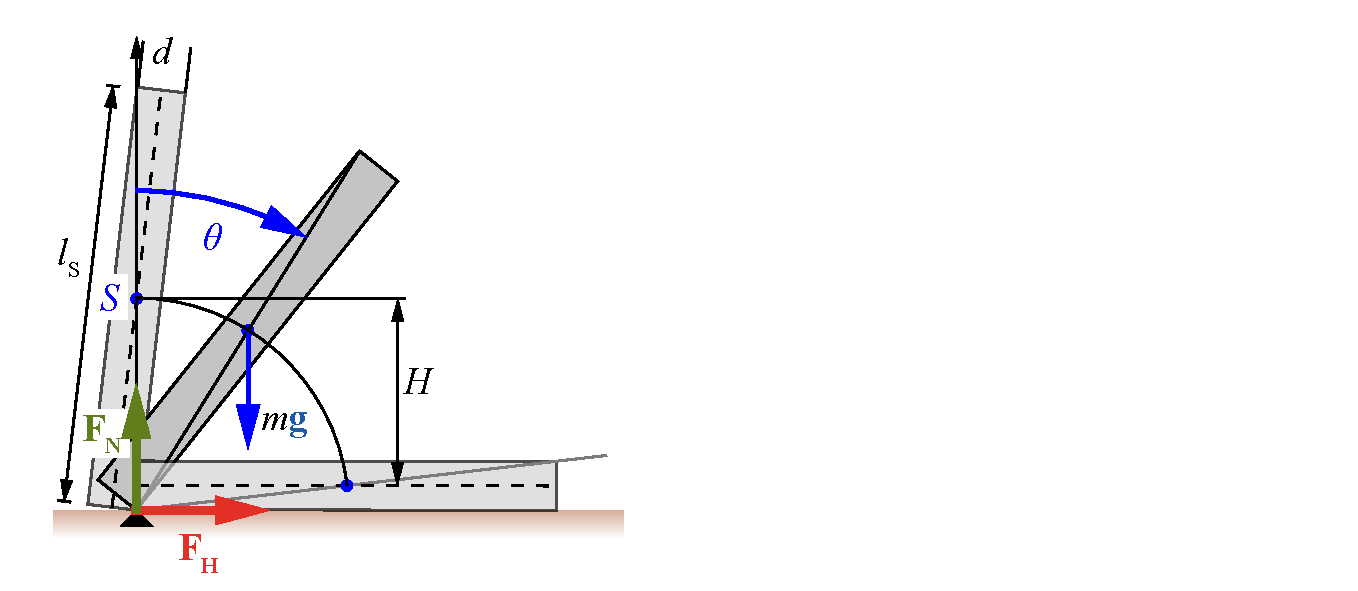
\includegraphics[width=\textwidth]{FallingRod08.pdf}
  \caption[Geometrie beim umfallenden Smartphone.]{Geometrie und physikalische Gr��en beim umfallenden Smartphone.} \label{abb:bew_fallingrod08}
\end{figure}

\newpage 

\subsection{Physikalische Kreisel-Spielzeuge und verwandte Themen} \label{kap:bew_apps_top}


\subsubsection{Rollende Zylinder, Garnrollen, Jo-Jos}

Der rollende Zylinder und das Jo-Jo sind in Lehrb�chern oft behandelte
Probleme. Generell sind physikalische Spielzeuge ungemein instruktiv und man
gewinnt auch ohne analytische Behandlung oft sehr tiefe Einblicke in und ein
intuitives Verst�ndnis f�r die grundlegenden Gesetze der Physik.
Wir empfehlen als Einstiegsliteratur besonders \cite{Ucke2011, Schlichting2016} und 
wollen hier einige der bekannten und weniger bekannten Effekte
etwas analytischer und auch quantitativer betrachten.

\subparagraph{\textbf{Garnrolle}}

    Wir beginnen zun�chst mit dem in vielen Lehrb�chern behandelten Beispiel
    der Garnrolle, das \ua f�r das Verst�ndnis des Jo-Jos hilfreich ist.
    Wie man an \figref{bew_Zylinder01} sieht, ist in beiden F�llen (a,b) das Drehmoment
    \[
    \vec{M}_\text{D}=\vec{r}\times\vec{F}
    \]
    so gerichtet, dass die Garnrolle nach rechts rollt. Im Fall c ist beim Grenzwinkel
    \[
    (90\,^\circ-\theta_\text{C}) = \arcsin\frac{R_i}{R_a}
    \]
    kein Rollen m�glich, da das Drehmoment in dieser Situation 0 ist,
    f�r $\theta>\!\theta_\text{C}$ wird die Garnrolle nach links rollen.

\begin{figure}
  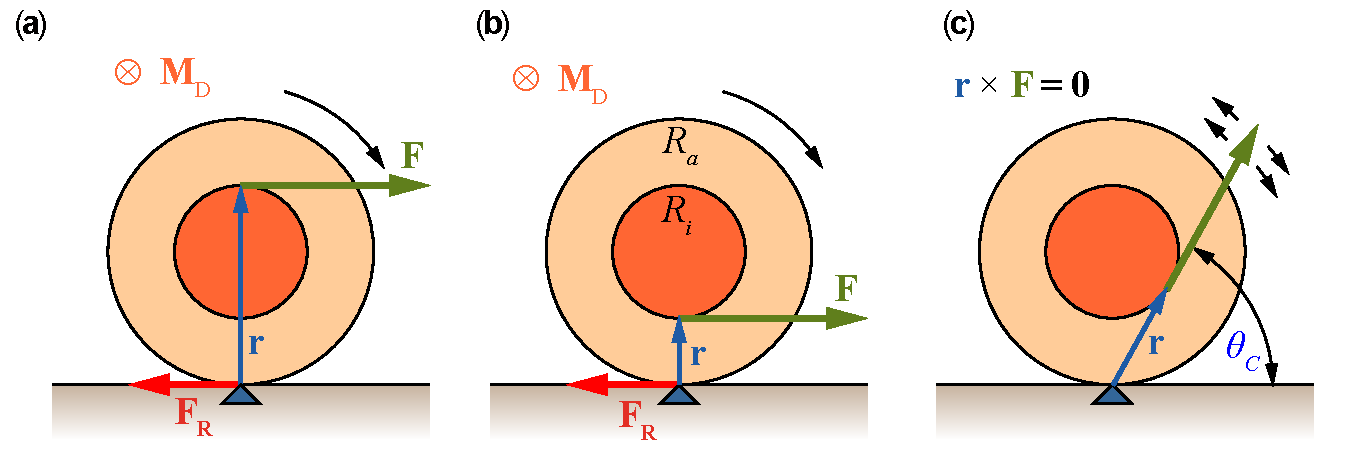
\includegraphics[width=\textwidth]{Garnrollen.pdf}
  \caption[Drehmomentwirkung an einer Garnrolle.]{Drehmomentwirkung an einer Garnrolle. H�ufig gestellte Quizfrage: Wohin rollt die Garnrolle? \fa \fb In beiden F�llen rollt die Garnrolle (sofern man nicht zu heftig daran zieht) nach rechts. \fc Ab einem kritischen Winkel $\theta_\text{C}$ wird die Garnrolle nach links rollen.} \label{abb:bew_Zylinder01}
\end{figure}

\subparagraph{\textbf{Jo-Jo}} \label{kap:bew_JoJo}
	
	Das Jo-Jo und das verwandte Diabolo (\figref{bew_Zylinder10}\,a,b) waren und sind zwei beliebte physikalische Spielzeuge, die dennoch relativ selten in der physikalischen Lehrliteratur behandelt werden.
        Die Zwangsbedingungen f�r die Bestimmung der Lagrange-Funktion des Jo-Jos (\figref{bew_Zylinder10}) haben wir bereits in \probref{bew_Zwangsbedingungen} hergeleitet. 

\begin{figure}
  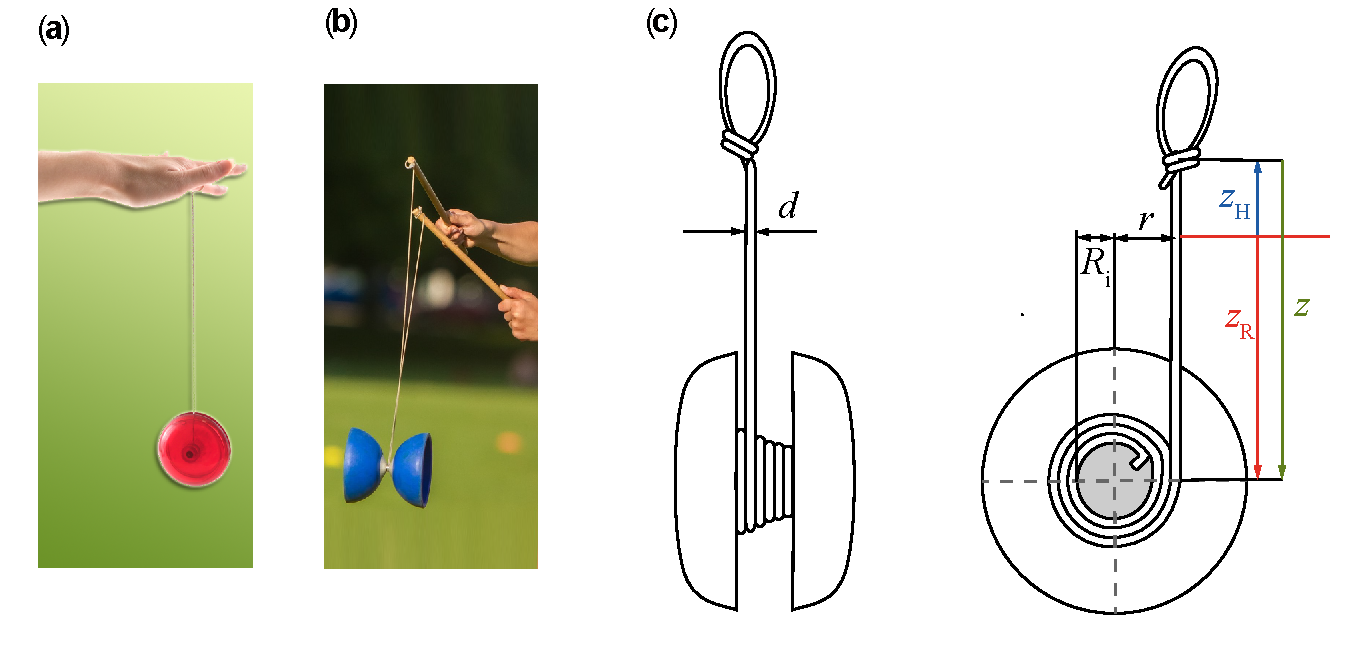
\includegraphics[width=\textwidth]{Zylinder10.pdf}
  \caption[Geometrische und physikalische Gr��en des Jo-Jos.]{Geometrische und physikalische Gr��en des Jo-Jos. \fa �bliche Ausf�hrungsform des Jo-Jos. \fb Verwandt mit dem Jo-Jo ist das Diabolo, dass aus einem Doppelkegel besteht, welcher auf ein Seil gesetzt wird, das an seinen Enden an zwei Handst�cken befestigt ist. Durch Bewegen des Seils wird das Diabolo in Rotation versetzt und damit als Kreisel im Raum stabilisiert.  \fc Im linken Teil des Bildes ist der Fadenkanal des Jo-Jos zu sehen, im rechten Teil des Bildes die Definition der im Folgenden verwendeten Gr��en: $R_\text{i}$ Wellenradius, $r=r(z)$ Spulenradius, $d=d_\text{eff}$ effektive Fadendicke, $z_\text{F}$ Fallh�he, $z_\text{H}$ Steuergr��e der Hand und $z$ Abwickell�nge des Jo-Jos (nach \cite{Buerger1983}).}
	\label{abb:bew_Zylinder10}
\end{figure}

	Dort haben wir aber die Fadendicke als Null angenommen.
    Diese wollen wir jetzt ber�cksichtigen und auch, dass mehrere Lagen des aufgewickelten
    Fadens �bereinander auf dem Wellenk�rper Platz finden (\figref{bew_Zylinder10}\,c). Daraus resultiert ein ver�nderlicher Spulenradius $r=r(z)$, ebenso wie eine effektive Fadenl�nge. Aus (\figref{bew_Zylinder10}\,c) sehen wir, dass sich bei einer regelm��igen Wicklung eine \anf{effektive Dicke} $d_\text{eff}$ des Fadens einf�hren l�sst, die durch
    \begin{align}
      \pi r^2 = \pi R_\text{i}{}^2 + d_{\text{eff}} \,(l_\text{S}-z) \label{eq:bew_JoJo01}
    \end{align}
    gegeben ist \cite{Buerger1983}. $l_\text{S}$ ist die Gesamtl�nge der Schnur und es gilt
    \[
    r_{\min} = r(z=l_\text{S}) = R_\text{i},\quad \text{\bzw} \quad r_{\max}=r(z=0) = \sqrt{R_\text{i}{}^2 + d_{\text{eff}} \,l_\text{S}/\pi }\,.
    \]
    Typische Werte sind $r_{\min}=\SI{0.3}{\centi\metre}$ und  $r_{\max}=\SI{1.3}{\centi\metre}$
    f�r $l_\text{S}=\SI{100}{\centi\metre}$, womit $d_{\text{eff}}=\SI{0.05}{\centi\metre}$ gilt.
    Die Lagrange-Gleichung 1.\ Art lautet dann
    \begin{align}
      m\ddot z&=mg-F_\text{T} ~~~\text{mit}~~~J\frac{\ddot z}{r^2(z)} = F_\text{T}\,,  \label{eq:bew_JoJoLGL}
    \end{align}
    wobei die Zwangsbedingung hier die Rollbedingung ist und die Zwangskraft $F_\text{T}$, die das Drehmoment auf die Jo-Jo-Scheibe verursacht.
    F�r das Jo-Jo nehmen wir zun�chst die Hand als ruhend an ($z_\text{H} = 0$).
    In diesem Fall ist $z_\text{F}=z$ und indem wir $\ddot z$ eliminieren, erhalten wir $F_\text{T}(z)$:
    \begin{align}
      F_\text{T}(z) = m g \frac{1}{1+m\,r(z)^2/J} = m g\frac{1}{1+2r(z)^2/R_a{}^2}\,~~\text{f�r}~~J\approx \frac 12\,m\, R_a{}^2\,. \label{eq:bew_JoJo08}
    \end{align}
    Dies gilt f�r $z\leq l_\text{S}$. 
    Da wir zun�chst Energieerhaltung annehmen, k�nnen wir schreiben:
    \begin{align}
      \frac m2v^2+\frac {J}{2}\omega^2-mg z = E\,.\label{eq:bew_JoJo02}
    \end{align}
    Hierin ist $v=\dot{z}$ die Schwerpunktsgeschwindigkeit,
    die beim einfachen Fallen, \dh ohne Steuerung durch die Hand,
    wegen $z=z_\text{F}$ nach der Fallstrecke $z$ erreicht wird.
    Aus der Rollbedingung $|v|=r|\omega |$ folgt dann
    \begin{align}
      v (z) =\pm\sqrt{2gz}\frac1{\sqrt{1+J/\lk mr^2(z)\rk}}\,,\label{eq:bew_JoJo03}
    \end{align}
    das Jo-Jo f�llt also durch das Wirken der Fadenspannung langsamer als ein frei fallender K�rper, was leicht einsichtig ist, da ja auch Energie in Rotation
    umgesetzt wird. Die Geschwindigkeit erreicht ein Maximum und f�llt dann wieder ab
    (\figref{bew_Zylinder11}).%
    \footnote{Streng genommen ist $J$ auch eine Funktion von $z$.
    Wenn wir die Masse des Fadens als sehr viel kleiner
    als die Masse der Jo-Jo Scheibe annehmen,
    k�nnen wir aber $J$ als konstant annehmen.}

\begin{figure}
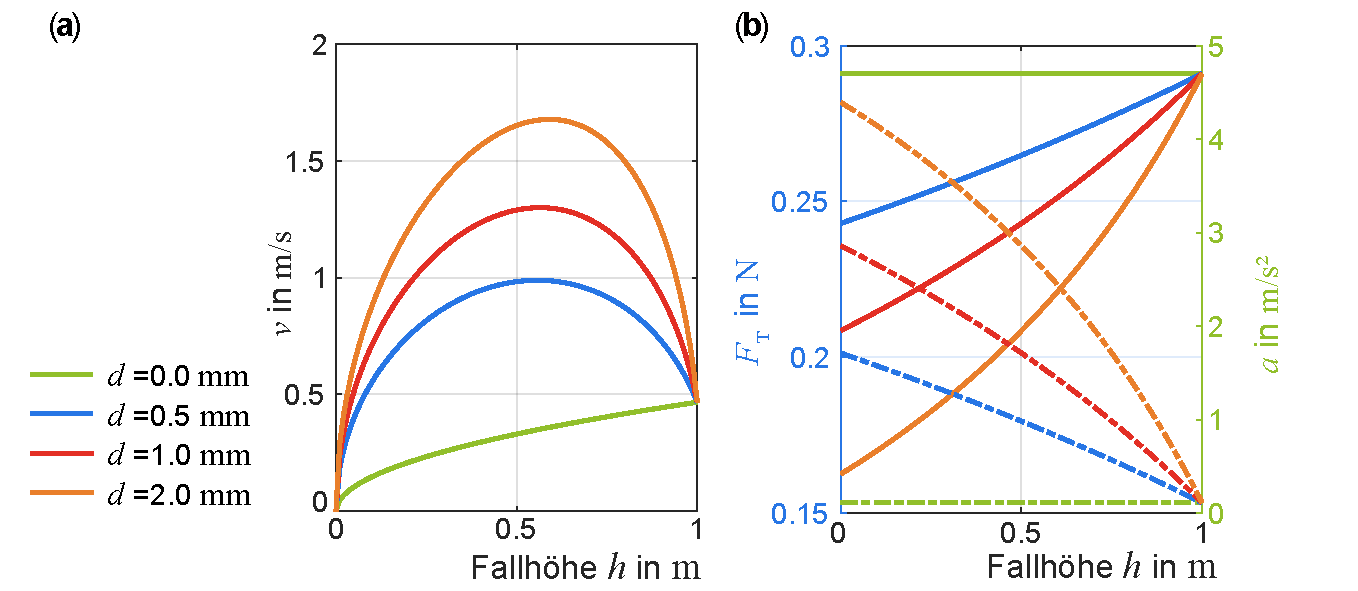
\includegraphics[width=\textwidth]{Zylinder11.pdf}
\caption[Geschwindigkeit, Fadenspannung und Beschleunigung des Jo-Jos.]{\fa Geschwindigkeit, sowie \fb Fadenspannung und Beschleunigung des Jo-Jos als Funktion der H�he. Als Parameter ist die Fadendicke $d$ angegeben. Die gr�ne Kurve beschreibt f�r eine effektive Fadendicke von Null das sogenannte akademische Jo-Jo.} \label{abb:bew_Zylinder11}
\end{figure}

    Wir schreiben Gl. \eqref{eq:bew_JoJo03} als
    \begin{align}
      \D t = \frac{\D z}{\sqrt{2gz}}\sqrt{1+ J/\lk mr^2(z) \rk}\,,
      \label{eq:bew_JoJo04}
    \end{align}
    substituieren
    \begin{align*}
      r^2(z) &= R_\text{i}{}^2+d(l_\text{S}-z)\,,~~ z = \frac{\pi r_{\max}{}^2}d\sin^2\psi\,,\\
			\phi &= \arccos\frac{r_{\min}}{r_{\max}}\,~~ \text{und}~~
			k=\frac{1}{\sqrt{1+J/\lk m\,r_{\max}{}^2 \rk}}\,,
    \end{align*}
    und erhalten nach Integration (Nachrechnung in \probref{bew_JoJoDynamik})
    \begin{align}
      t=\bigintsss_{\,0}^{t} \D t^\prime=\sqrt{\frac{2\pi}{g\,d}}\frac{r_{\max}}k
      \bigintsss_{\,0}^\phi \sqrt{1-k^2\sin^2\psi}\:\D \psi = E(\phi,k)\,.
      \label{eq:bew_JoJo05}
    \end{align}
    $E(\phi,k)$ ist das \textit{elliptisches Integral der 2. Art} \index{Integral!elliptisches} \cite{Gradshteyn1980, Olver1992}, das auch in \matlab{} hinterlegt ist.
    Alternativ l�sst sich nat�rlich auch \eqref{eq:bew_JoJoLGL} numerisch integrieren (\mscr{} \mlbewref{JoJo01.m})
    Damit haben wir die Phase des Abspulens beschrieben,
    da die Umkehrung von $t=t(\psi(z))$ uns $z(t)$ liefert.

    Ist das Jo-Jo abgespult $(t=t_u,\, z=l_\text{S})$, dann wendet das Jo-Jo
    (\figref{bew_Zylinder13}) und die Bewegung des Jo-Jos wird jetzt
    durch eine Drehung �ber
    \[
    z=l_\text{S}+R_\text{i}\cos\varphi  ~~~\text{mit}~~~ -\pi/2 \leq \varphi \leq \pi/2
    \]
    beschrieben. In dieser Phase kann man das Jo-Jo als physikalisches Pendel betrachten
    \cite{Minkin2021}.
 %
\begin{figure}
\begin{minipage}{\textwidth}
\leftfigure{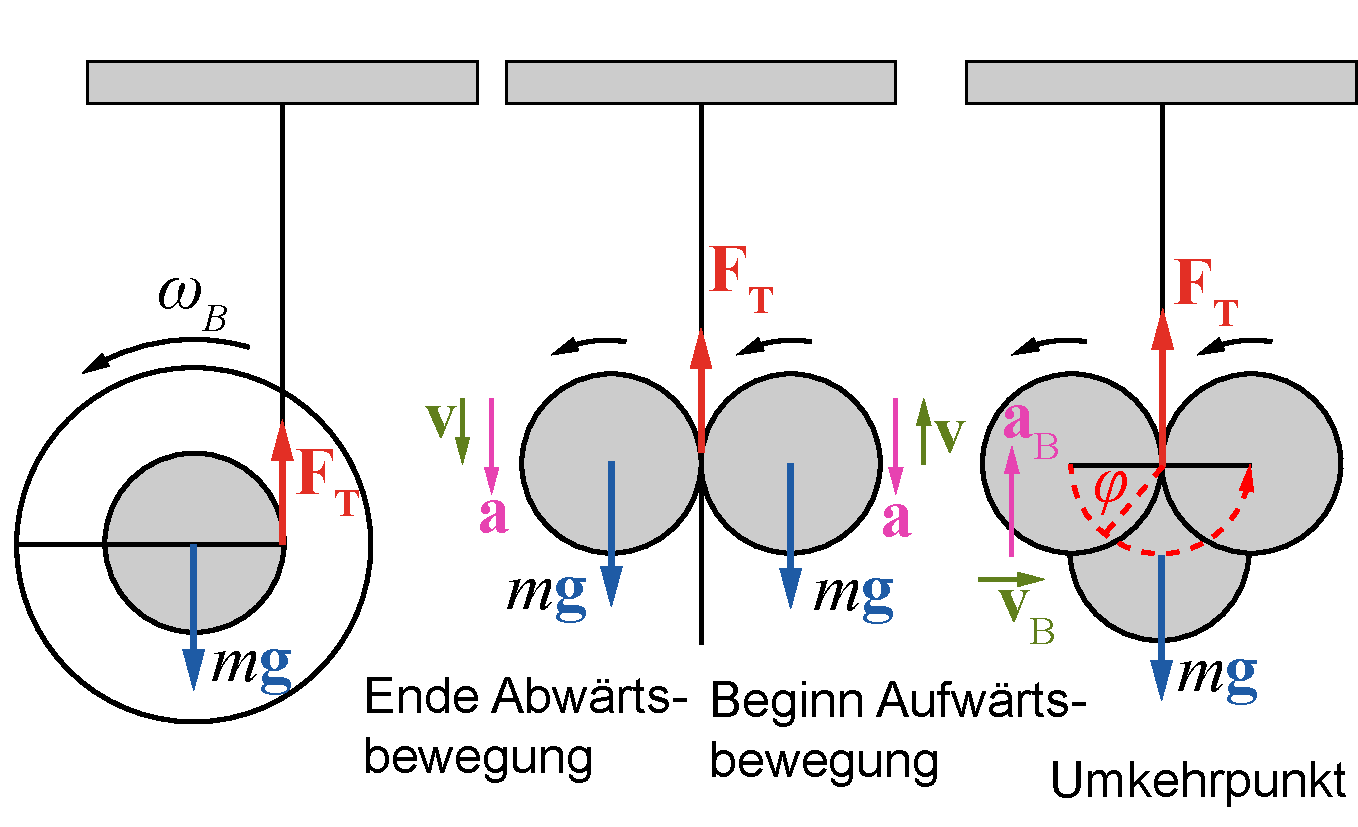
\includegraphics[width=0.5\textwidth]{Zylinder13.pdf}}%
\hspace{\fill}
\rightfigure{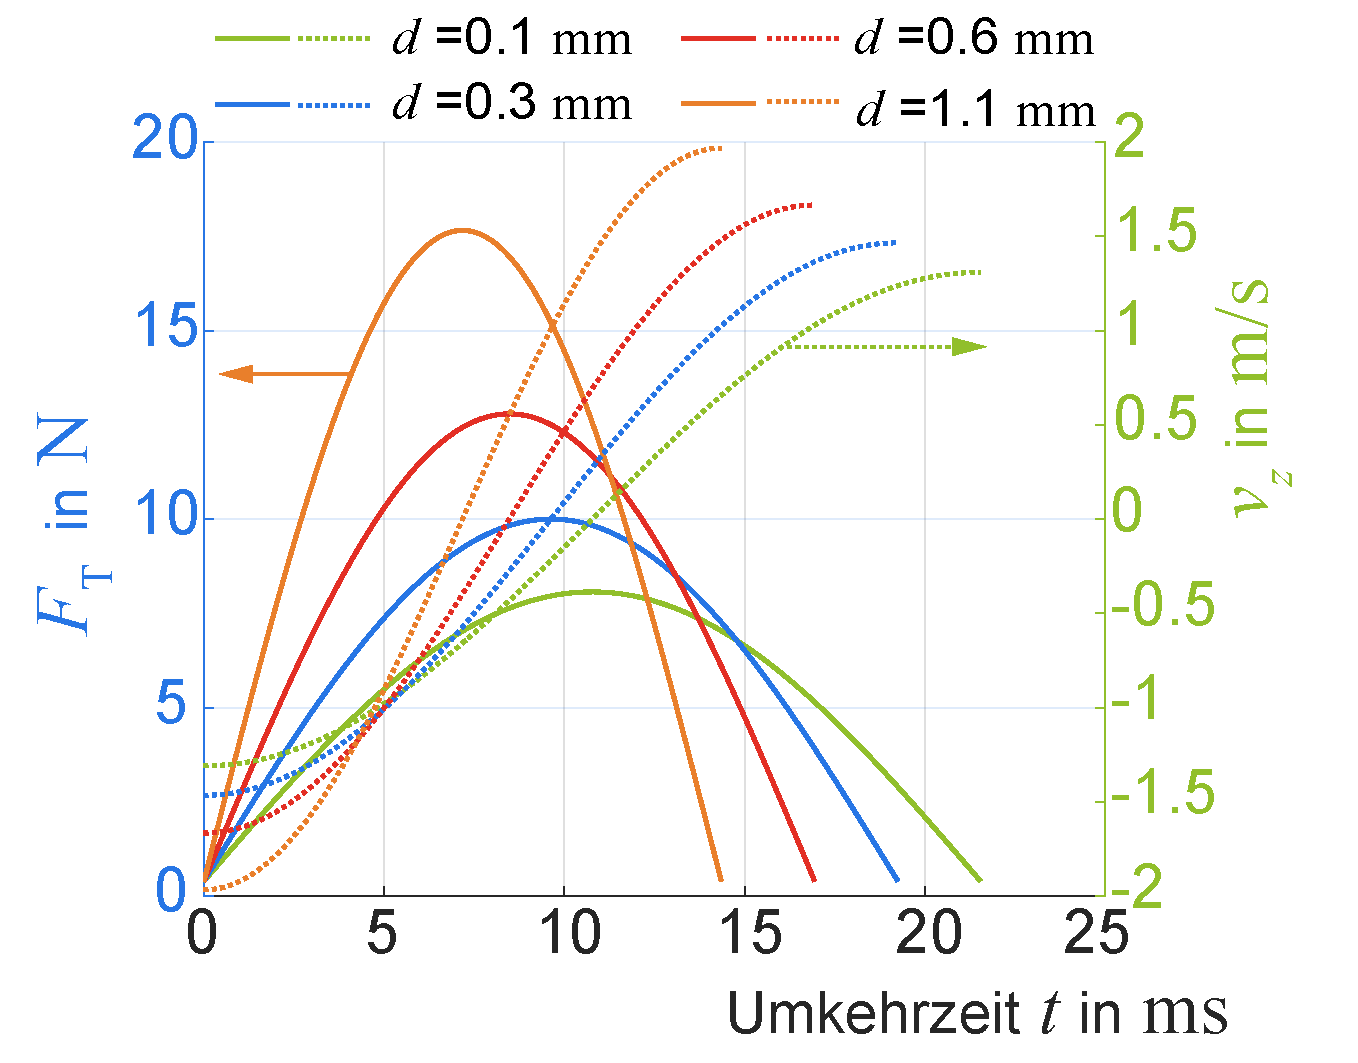
\includegraphics[width=0.5\textwidth]{Zylinder14.pdf}}
\leftcaption[Verhalten des Jo-Jos am Wendepunkt.]{Verhalten des Jo-Jos am Wendepunkt. Das Jo-Jo verh�lt sich wie ein physikalisches Pendel. $\vec{F}_\text{T}$ ist die Zugspannung im Faden, $\vec a$ die Beschleunigung, $\vec v$ die Geschwindigkeit des Massenmittelpunktes. Am Umkehrpunkt addiert sich die Zentripetalbeschleunigung zu $\vec g$ hinzu.} \label{abb:bew_Zylinder13}
\rightcaption[Fadenspannung und Geschwindigkeit des Jo-Jos am Wendepunkt.]{Fadenspannung und Geschwindigkeit des Jo-Jos am Wendepunkt.} \label{abb:bew_Zylinder14}
\end{minipage}
\end{figure}

    Wie in \figref{bew_Zylinder13} gezeigt, rotiert der Jo-Jo-K�rper um den mehr oder weniger
    gestreckten Faden.\footnote{Das ist umso mehr erf�llt, je l�nger der Faden ist, also wenn
    $l_\text{S}\gg R_\text{i}$.} Die halbe Schwingungsfrequenz $\omega_B$ kann man aus der Energieerhaltung f�r das physikalische Pendel gewinnen:
	\[ \omega_B = \sqrt{\frac{2mg l_\text{S}}{J}} \sqrt{\frac{1+\frac{R_\text{i}}{2} \cos\varphi}{1+\frac{mR_\text{i}{}^2}{J} \sin\varphi}} \approx \sqrt{\frac{2mg l_\text{S}}{J}} \; .
	\]
        Man kann also die Kreisfrequenz also n�herungsweise als konstant ansehen. Damit ergeben sich \anf{Wendezeiten} $T_P=\pi/\omega_B$ von wenigen $\SI{}{\milli\s}$ und f�r die Tangentialgeschwindigkeit $v_B$ \bzw die Zusatzbeschleunigung $a_B$ am unteren Umkehrpunkt damit
   \begin{align}
     v_B \approx \omega_B\,R_\text{i} ~~\text{\bzw} ~~ a_B \approx \omega_B{}^2\,R_\text{i}\,. \label{eq:bew_JoJo07}
   \end{align}
	  Der Jo-Jo-Spieler wird dieses Umkehren durch einen kr�ftigen Zug am Faden, also in der Fadenspannung merken. 
    In der Umkehrphase f�r $z>l_\text{S}$ m�ssen wir also die $z$-Komponente der radialen Zentripetalkraft zur Fadenspannung \eqref{eq:bew_JoJo08} addieren.
    Wir berechnen $z(t)$ f�r $z\leq l_\text{S}$ aus der Lagrange-Gleichung \eqref{eq:bew_JoJoLGL} und f�r $z>l_\text{S}$ aus der L�sung f�r
    das physikalische Pendel \eqref{eq:bew_PhysPendel02} mit der Anfangsgeschwindigkeit $v_u$ und der Auslenkung $-\pi/2$.
    Das Ergebnis ist in \figref{bew_Zylinder14} dargestellt. Man erkennt, dass die Wendezeit
    nur einige Hundertstelsekunden betr�gt, die zus�tzliche Spannung im Faden wird entsprechend gro�.\\ 
		
    Zum Schluss wollen wir noch kurz das \anf{angeregte} Jo-Jo betrachten.
    Bei dieser Spielart ersetzt der Jo-Jo-Spieler den unvermeidbaren Reibungsenergieverlust beim Auf-und-Ab
    durch eine geschickt gesteuerte Bewegung des Fadenendes mit seiner Hand.
    F�r das getriebene Jo-Jo ist die Fallh�he $z_\text{R}$ im Raumkoordinatensystem dann verschieden von der Abwickell�nge $z$.
    Es gilt  $z=z_\text{R}+z_\text{H}$
    (\figref{bew_Zylinder11}), wo $z_\text{H}$ die Bewegung des Aufh�ngepunktes durch die steuernde Hand ist. Die Bewegungsgleichung gewinnt man unter Beachtung der Rollbedingung
    $|\dot z|=r|\dot\varphi|=\sqrt{R_\text{i}{}^2+(l_\text{S}-z)\, d/\pi}$
    aus der Lagrange-Funktion:
    \begin{align}
      \mathcal{L}_\text{S}(z,\dot z) = \frac m2\,(\dot z-\dot z_\text{H})^2
      + \frac J2\left(\frac{\dot z}r\right)^2 + m\,g\,(z-z_\text{H})\,,
      \label{eq:bew_JoJo09}
    \end{align}
    woraus wir die Lagrange-Gleichung
    \begin{align}
      \frac{\D}{\D t}\left[\left(1+\frac J{m\,r(z)^2}\right)\dot z^2\right]
      = 2\,(g+\ddot z_\text{H})\,\dot z \label{eq:bew_JoJo10}
    \end{align}
    gewinnen. Das l�sst sich integrieren: 
    \begin{align}
      \dot z^2 = \frac{2\left[g\,z+\bigintsss_{\,0}^t\ddot z_\text{H}(t')\,\dot{z}(t')\,\D t'+C\right]}{1+J/\lk mr^2(z) \rk}\,.
      \label{eq:bew_JoJo11}
    \end{align}
    $C$ ist eine Integrationskonstante, die sich aus den Anfangsbedingungen ergibt.
    Die Anregungsgr��e $z_\text{H}(t)$ bestimmt also die Bewegung des Jo-Jos, genauer das Integral
    \[
    \bigintsss_{\,0}^t\ddot z_\text{H}(t')\,\dot{z}(t')\,\D t' = \bigintsss_{\,0}^z\ddot z_\text{H}(z^\prime)\,\D z^\prime\,,
    \]
    welches die Energiezufuhr pro Masseneinheit auf dem durchlaufenen Weg der Jo-Jo-Schnur bedeutet.
    Energiezufuhr hei�t $\ddot z_\text{H}>0$, \dh eine Beschleunigung der Hand nach oben, wenn $z$ w�chst
    (Abwicklungsphase) und $\ddot z_\text{H}<0$ f�r $\dot z<0$ (Aufwicklungsphase).
    In \probref{bew_JoJoDynamik} wird die Dynamik des Jo-Jos $z(t)$ als Funktion der 
    Anregungsfunktionen $z_\text{H}(t)$ berechnet. Man erkennt, wie wichtig die Synchronisation der Hand mit der 
    Auf-und-Abbewegung des Jo-Jos ist (siehe auch \mscr{} \mlbewref{JoJo02.m}).


\subsubsection{Rollende Zylinder, Scheiben und Reifen} \label{kap:bew_rolling_disc}

\subparagraph{\textbf{Rollende Zylinder auf der schiefen Ebene}}	

Die Bewegung rollender Objekte auf der schiefen Ebene schafft es trotz ihrer
Einfachheit immer wieder zu faszinieren und manchmal mit der Intuition auf falsche Schl�sse zu kommen.
Typischerweise betrachtet man mehrere Objekte derselben
Masse und desselben Radius, aber unterschiedlicher Masseverteilung. L�sst man
sie die Ebene hinunterrollen, stellt sich die Frage, welches Objekt am
ehesten unten ankommt. Das wollen wir f�r die Hohlkugel, die Vollkugel,
einen Hohlzylinder, einen Vollzylinder und einen mit Fl�ssigkeit gef�llten
Zylinder betrachten. Dazu f�hren wir auf der schiefen Ebene
(\figref{bew_Zylinder05}) eine Koordinate $s$ entlang der Ebene ein, die an der
oberen Kante beginnt. $s$ stehe senkrecht auf dieser Kante.

\begin{figure}
  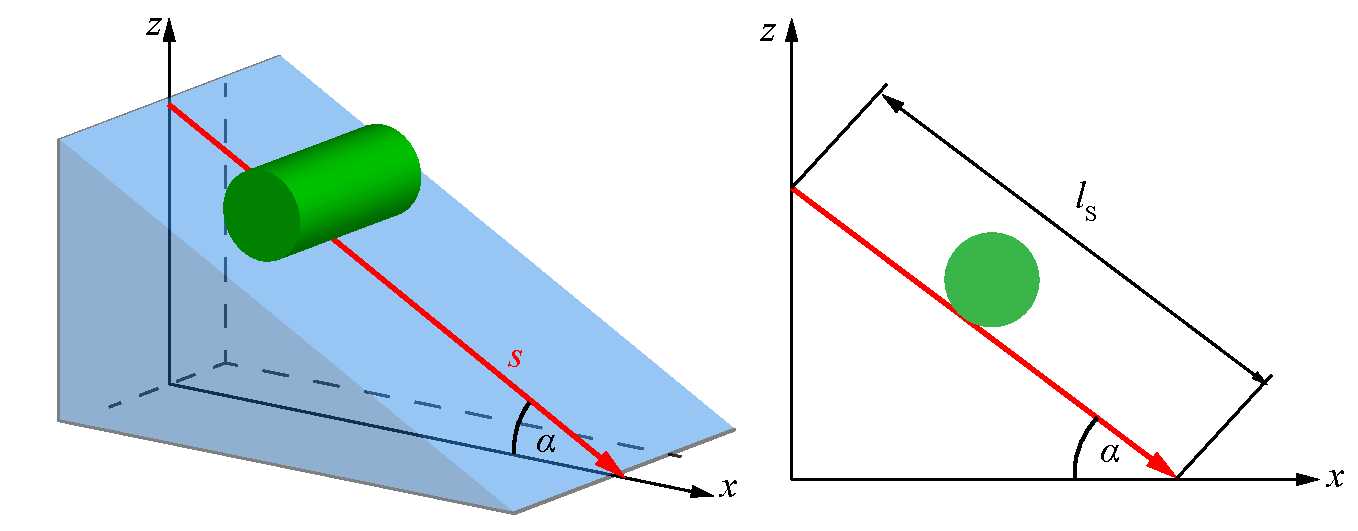
\includegraphics[width=\textwidth]{RollZylGeometrie.pdf}
  \caption[Geometrie des rollenden Zylinders.]{Geometrie des rollenden Zylinders.} \label{abb:bew_Zylinder05}
\end{figure}

Die Koordinate $s$ ist gut zur Beschreibung des Problems geeignet, denn zum
Aufstellen der Lagrange-Funktion ben�tigen wir die Translations- und
Rotationsenergien,
\begin{equation*}
  T = \frac{1}{2} m \dot{s}^2 + \frac{1}{2} J \omega^2 \; .
\end{equation*}
Wir wollen zun�chst davon ausgehen, dass die Reibung so stark ist, dass keines
der Objekte zu rutschen beginnt. Dann gilt die Rollbedingung $s = R \varphi$
mit dem identischen Radius $R$ aller Objekte. Aus dieser folgt $\omega =
\dot{\varphi} = \dot{s}/R$ und somit f�r die kinetische Energie
\begin{equation*}
  T = \frac{1}{2} m \dot{s}^2 + \frac{1}{2} \frac{J}{R^2} \dot{s}^2
  = \frac{1}{2} \left ( m + \frac{J}{R^2} \right ) \dot{s}^2 \; .
\end{equation*}
Das Potential ergibt sich zu
\begin{equation*}
  U = mg z  = mg (l_\text{S}-s) \sin\alpha
\end{equation*}
mit der Gesamtl�nge $l_\text{S}$ der Ebene. Es folgen die Lagrange-Funktion
\begin{equation*}
  \mathcal{L} = \frac{1}{2} \left ( m + \frac{J}{R^2} \right ) \dot{s}^2
  - mg (l_\text{S}-s) \sin\alpha
\end{equation*}
und die Bewegungsgleichung
\begin{equation*}
  \ddot{s} = \frac{mg}{m+J/R^2} \sin{\alpha} \;. 
\end{equation*}
Lassen wir alle Objekte an der oberen Kante ohne Anfangsgeschwindigkeit
starten, gilt $s(0) = \dot{s}(0) = 0$ und die L�sung der Bewegungsgleichung
lautet
\begin{equation*}
  s(t) = \frac{1}{2} \frac{mg}{m+J/R^2} \, t^2 \,\sin{\alpha}\;,
\end{equation*}
\bzw wir extrahieren daraus sofort die Zeit $t_L$, die das Objekt
ben�tigt, um die Strecke $l_\text{S}$ zur�ckzulegen und unten anzukommen,
\begin{equation*}
  t_L = \sqrt{ \frac{2 l_\text{S} \left ( m+J/R^2\right )}{mg
      \sin\alpha}} \;.
\end{equation*}

Es ist zu erwarten, dass das Objekt mit dem geringsten Tr�gheitsmoment die
k�rzeste Zeit ben�tigt. Hier geht am wenigsten Energie in die Rotation und
die meiste Energie steht f�r die Translationsbewegung zur Verf�gung. Folglich
kommt das Objekt am ehesten unten an. Aus den Tr�gheitsmomenten folgt dann als 
Reihenfolge (vergleiche �bung
\ref{prob:bew_traegheitsmomente}) f�r die Ankunft am unteren Ende:

\begin{enumerate}
\item Vollkugel, $J = \frac{2}{5} m R^2$
\item Vollzylinder, $J = \frac{1}{2} m R^2$
\item Hohlkugel mit Schalendicke $d \ll R$, $J = \frac{2}{3} m R^2$
\item Hohlzylinder mit Manteldicke $d \ll R$, $J = m R^2$
\end{enumerate}

Au�en vor gelassen haben wir bisher den mit einer Fl�ssigkeit gef�llten
Hohlzylinder. Dieser ist in unserer bisherigen Betrachtung noch nicht
enthalten, denn wir sind von einem starren K�rper ausgegangen, dessen gesamte
Masse immer der Drehbewegung folgt. Das ist hier jedoch nicht erf�llt. Die
Fl�ssigkeit beginnt zwar durch die Reibungskr�fte am Rand, sich ebenfalls
zu bewegen, tut das jedoch nur langsam. Da die Drehbewegung des Rands immer
schneller wird, wird die Fl�ssigkeit sich zu jedem Zeitpunkt langsamer drehen als die
H�lle. Es geht hier also deutlich weniger Energie in die Rotation als beim
entsprechend schweren Vollzylinder. Die Einsortierung in die oben genannte
Reihenfolge h�ngt nat�rlich davon ab, wie gro�
die Z�higkeit\index{Viskosit�t}\index{Z�higkeit} der Fl�ssigkeit
und der Massenanteil der H�lle
ist, denn diese stellt eine Art Hohlzylinder dar. Typischerweise liegt jedoch
der gr��te Teil der Masse -- man denke \zb an eine Konservendose -- in der
Fl�ssigkeit. In diesem Fall kann der fl�ssigkeitsgef�llte Zylinder durchaus
das schnellste Objekt sein. 

\subparagraph{\textbf{Rollende Scheiben und Reifen auf einer Ebene}}	

Wir wollen nun einen Schritt weiter gehen und rollende R�der \bzw Reifen
betrachten. Dies ist ein oft behandeltes
Beispiel. Wir wollen hier die wesentlichen Punkte, die f�r das Verst�ndnis wichtig
sind, nachvollziehen und verweisen f�r einige wenige ausgelassene Rechenschritte den interessierten
Leser auf die Literatur. Ausf�hrliche Darstellungen finden sich \zb in \cite{Kuypers2012, Morin2008}.
Der Einfachheit halber modellieren wir diese durch eine
Kreisscheibe. Das Problem ist im Wesentlichen dasselbe, nur die
Tr�gheitsmomente unterscheiden sich, weil bei einem Rad der gr��te Teil der
Masse am �u�eren Radius konzentriert ist. \\
Im Gegensatz zu Zylindern tritt bei R�dern oder Kreisscheiben ein weiterer
Freiheitsgrad auf. Zylinder liegen immer stabil mit einer Achse parallel zur
Figurenachse auf dem Boden auf. Bei einer Kreisscheibe ist das nicht so, diese
kann umkippen und ihre Lage im Raum muss gesondert betrachtet werden, wie in \figref{bew_LageKreisscheibe} dargestellt.

\begin{figure}
  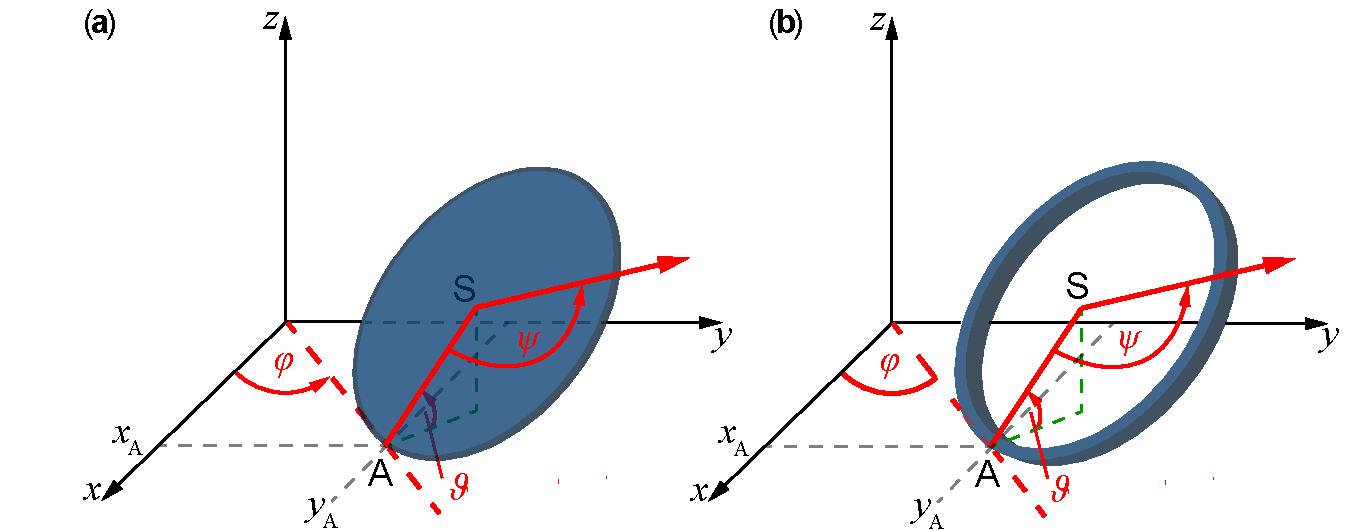
\includegraphics[width=\textwidth]{KreisscheibeLage.pdf}
  \caption[Rollende Kreisscheiben und Ringe.]{Rollende Kreisscheiben und Ringe.
    Da Kreisscheiben und Ringe ideale symmetrische Kreisel darstellen, die
    sich prinzipiell um alle drei Achsen frei drehen k�nnen, sind die Eulerwinkel
    $\varphi$, $\vartheta$, $\psi$ ideal zur Beschreibung ihrer jeweiligen Lage geeignet.}
  \label{abb:bew_LageKreisscheibe}
\end{figure}

Wir verwenden f�r die Beschreibung der Lage der Kreisscheibe die drei
Eulerwinkel $\varphi$, $\vartheta$, $\psi$ aus
\kapitel{bew_EulerWinkel}. Sie sind ideal geeignet, da die Kreisscheibe einen
symmetrischen Kreisel darstellt, der sich prinzipiell um alle drei Achsen
frei bewegen kann. Die einzige Einschr�nkung besteht darin, dass wir sie
immer auf dem Boden, \dh in der $x$-$y$-Ebene rollen lassen wollen. 
Dadurch ergibt sich eine Zwangsbedingung, die die Koordinaten
$x_\mathrm{A}$ und $y_\mathrm{A}$ des Auflagepunktes mit den Eulerwinkeln
verkn�pft. Diese Relation kann jedoch nur differentiell angegeben werden,
da sich alle Variablen mit der Zeit �ndern,
\begin{subequations}
  \begin{align}
    \D x_\mathrm{A} &= - R \cos\varphi\, \D \psi \qquad \text{bzw.} \qquad
                      \dot{x}_\mathrm{A} + R \cos\varphi\, \dot{\psi} = 0 \; ,
                      \label{eq:bew_ZBrollendeScheibe1} \\
    \D y_\mathrm{A} &= - R \sin\varphi\, \D \psi \qquad \text{bzw.} \qquad
                      \dot{y}_\mathrm{A} + R \sin\varphi\, \dot{\psi} = 0 \; .
                      \label{eq:bew_ZBrollendeScheibe2}
  \end{align}
\end{subequations}
Dies ist ein typisches Beispiel f�r eine nicht-holonome Zwangsbedingung.

Die Rotationsenergie l�sst sich mit den Tr�gheitsmomenten $J_1 = J_2 = J_{12}$
und $J_3$ im k�rperfesten System mit $T_\mathrm{rot} = \frac{1}{2} J_{12}
( \omega_1'^2 + \omega_2'^2 ) + \frac{1}{2} J_3 \omega_3'^2$ angeben. Mit
\eqref{eq:bew_EulerWinkel} ergibt sich daraus
\begin{align}
  T_\mathrm{rot} &= \frac{1}{2} J_{12} \left ( \dot{\vartheta}^2 + \sin^2
  \vartheta \, \dot{\varphi}^2 \right ) +  \frac{1}{2} J_{3} \left (
  \cos^2 \vartheta \, \dot{\varphi}^2 + 2 \cos\vartheta\, \dot{\varphi} \dot{\psi}
                   + \dot{\psi}^2 \right ) \notag \\
  \intertext{\bzw mit $J_{12} = mR^2/4$ und $J_3 = mR^2/2$ f�r eine Kreisscheibe}
  T_\mathrm{rot} &= \frac{mR^2}{8} \left ( \dot{\vartheta}^2 + ( 1 + \cos^2
                   \vartheta ) \dot{\varphi}^2 +
                   4 \cos\vartheta\, \dot{\varphi} \dot{\psi}
                   + 2\, \dot{\psi}^2 \right ) \; .
                   \label{eq:bew_rollendeScheibe_rotE}
\end{align}

Hinzu kommt die Translationsenergie, die sich mit der Schwerpunktkoordinate
\begin{align*}
  x_\mathrm{S} &=  x_\mathrm{A} - R \cos\vartheta\,\sin\varphi \;, \quad
  y_\mathrm{S} =  y_\mathrm{A} + R \cos\vartheta\,\cos\varphi \;, \quad
  z_\mathrm{S} =  R \sin\vartheta
\end{align*}
zu
\begin{align}
\begin{split}
  T_\mathrm{trans} &= \frac{m}{2} \bigg ( \dot{x}_\mathrm{A}^2 +
    \dot{y}_\mathrm{A}^2 + R^2(\dot{\vartheta}^2 + \cos^2 \vartheta\,
    \dot{\varphi}^2 ) \\
		& \quad\quad\quad - 2 R \dot{x}_\mathrm{A} ( \cos\varphi\, \cos\vartheta\,
    \dot{\varphi} - \sin\varphi\, \sin\vartheta\, \dot{\vartheta} ) \\
    & \quad\quad\quad - 2 R \dot{y}_\mathrm{A} ( \sin\varphi\, \cos\vartheta\,
    \dot{\varphi} + \cos\varphi\, \sin\vartheta\, \dot{\vartheta} ) \bigg )
  \end{split}\label{eq:bew_rollendeScheibe_transE}
  \end{align}
ergibt, und das Potential
\begin{equation}
  U = m g z_\mathrm{S} =  m g R \sin\vartheta \; .
  \label{eq:bew_rollendeScheibe_Pot}
\end{equation}

Diese Gleichungen enthalten mit $x_\mathrm{A}$, $y_\mathrm{A}$, $\varphi$,
$\vartheta$ und $\psi$ f�nf Koordinaten, die jedoch nicht voneinander
unabh�ngig sind, sondern durch die differentiellen Zwangsbedingungen
\eqref{eq:bew_ZBrollendeScheibe1} und \eqref{eq:bew_ZBrollendeScheibe2}
miteinander verkn�pft sind. Die L�sung erfolgt deshalb �ber die Methode der Lagrange-Multiplikatoren 
�ber die Lagrange-Gleichungen erster Art (siehe \eqref{eq:bew_Lagrange_I} in \kap{bew_Lagrange_I}). Daraus lassen
sich f�r die drei Eulerwinkel die Differentialgleichungen
\begin{subequations}
  \begin{align}
    \sin\vartheta\, \ddot{\varphi} - 2 \dot{\psi}\dot{\vartheta} &= 0 \; , \\
    \ddot{\vartheta} +  \sin\vartheta\, \cos\vartheta\,
    \dot{\varphi}^2 + \frac{6}{5} \sin\vartheta\, \dot{\varphi}\,\dot{\psi}
    + \frac{4}{5} \frac{g}{R} \cos\vartheta &= 0 \; , \\
    \sin\vartheta\, \ddot{\psi} + \frac{5}{3}\, \sin^2\vartheta \ \dot{\varphi}\,
    \dot{\vartheta} + 2  \cos\vartheta\, \dot{\psi}\,\dot{\vartheta} &= 0 \;
                                                                       \label{eq:bew_ZBrollendeScheibe3}
  \end{align}
  \label{eq:bew_rollendescheibe_dgls}
\end{subequations}

ableiten, was wir in \probref{bew_scheibe} verifizieren wollen.
Die Position des Auflagepunktes $x_\mathrm{A}$,
$y_\mathrm{S}$ erh�lt man, indem man die Zwangsbedingungen
\eqref{eq:bew_ZBrollendeScheibe1} und \eqref{eq:bew_ZBrollendeScheibe2}
aufintegriert. 

\begin{figure}
  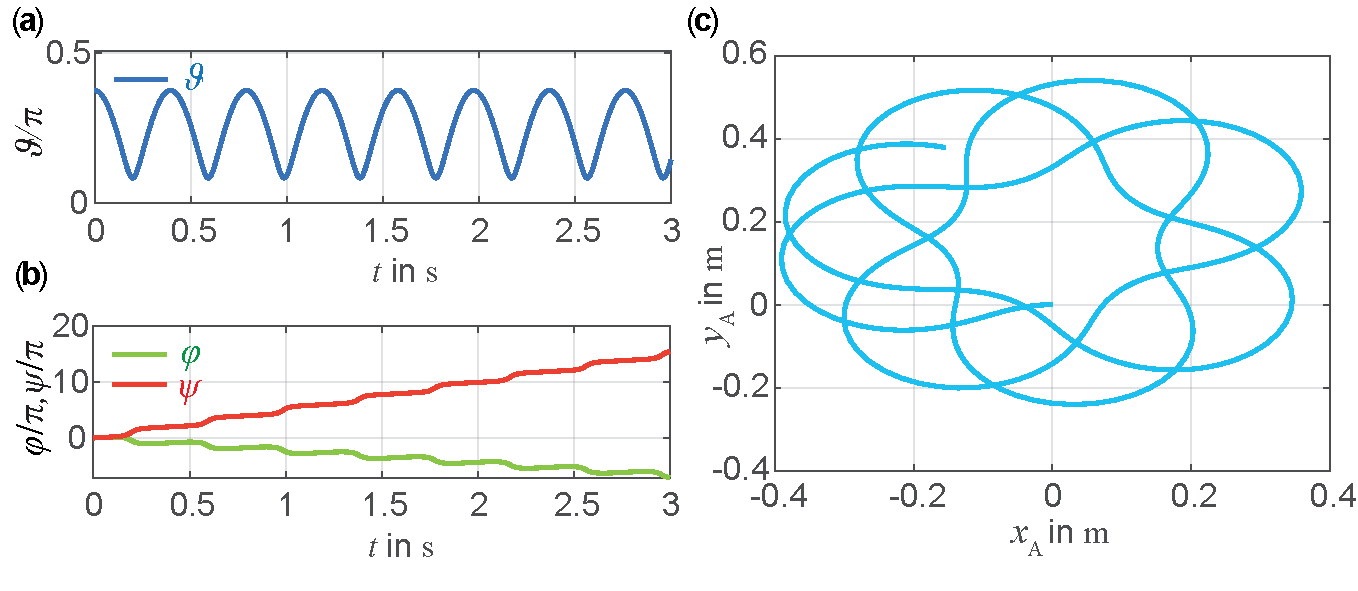
\includegraphics[width=\textwidth]{RollendeKreisscheibe.pdf}
  \caption[Bewegung einer rollenden Kreisscheibe.]{Bewegung einer rollenden
    Kreisscheibe mit $R=\SI{15}{\centi\metre}$ und den Anfangsbedingungen
    $\varphi = \psi = 0$, $\vartheta = 3\pi/8$, $\dot{\varphi} = \dot{\psi}
    = \SI{6}{\per\second}$, $\dot{\vartheta} = 0$ sowie $x_\mathrm{A}(0)
    =y_\mathrm{A}(0)=0$. \fa \fb Eulerwinkel und \fc Spur des Auflagepunktes in der $x$-$y$-Ebene. Die Scheibe beginnt zun�chst zu kippen. Dadurch
    steigt jedoch die Rollgeschwindigkeit und der Drehimpuls verhindert
    ein vollst�ndiges Umkippen. Die Schreibe richtet sich wieder auf. Dabei
    bewegt sie sich im Raum schlingernd fort.}
  \label{abb:bew_BewegungKreisscheibe}
\end{figure}

Diese Gleichungen wollen wir nun numerisch l�sen (siehe 
\mscr{} \mlbewref{RollendesRad.m}). F�r eine Kreisscheibe mit
dem Radius $R=\SI{15}{\centi\metre}$, die im
Ursprung startet ($x_\mathrm{A}(0)=y_\mathrm{A}(0)=0$), zu Beginn die
Neigung $\vartheta = 3\pi/8$ mit $\varphi = \psi = 0$ hat und sich mit den
Winkelgeschwindigkeiten $\dot{\varphi} = \dot{\psi} = \SI{6}{\per\second}$,
$\dot{\vartheta} = 0$ bewegt, ergibt sich der Fall, der in Abbildung
\figref{bew_BewegungKreisscheibe} dargestellt ist. Man erkennt deutlich in \figref{bew_BewegungKreisscheibe}a, wie die Kreisscheibe zun�chst beginnt zu kippen. Der
Winkel $\vartheta$ wird kleiner, was einer Ann�herung an die flach auf dem
Boden liegende Kreisscheibe entspricht. Dadurch wird die Rollbewegung jedoch
beschleunigt, die Ableitung der Winkel $\varphi$ und $\psi$ wird gr��er (\figref{bew_BewegungKreisscheibe}b).
Hier setzt sich nun der Drehimpuls durch. F�r ein weiteres Kippen m�sste (die
Scheibe rollt die ganze Zeit!) mehr kinetische Energie aufgebracht werden, als
durch das Gravitationspotential zur Verf�gung steht. Folglich kehrt die
Kippbewegung um und die Kreisscheibe richtet sich wieder auf. Das Spiel wiederholt sich mehrfach. Im Englischen wird das Ph�nomen \textit{wobbling disk} genannt.
Der Auflagepunkt legt dabei die Bewegung zur�ck, die in \figref{bew_BewegungKreisscheibe}c gezeigt ist. Man erkennt deutlich, wie die
Kreisscheibe sich in einer Schlingerbewegung vom Ursprung entfernt und sich
zeitweise wieder ann�hert. Sie umrundet dabei mehrfach ein sich langsam �nderndes Zentrum der Bewegung. 

Wir halten dabei fest, dass ein Rad zwar kippen kann, durch die Drehbewegung
und den dabei im System befindlichen Drehimpuls kann dieser Kippbewegung
jedoch eine Grenze gesetzt werden. Das Rad kann sich einigerma�en stabil
bewegen. Dies gilt umso mehr, je schneller es sich dreht. Wir werden darauf im Band III 
bei der Physik des Sports mehrfach zur�ck kommen.

\subsubsection{Der aufw�rts rollende Doppelkegel} \label{kap:bew_doublecone}

\subparagraph{\textbf{Grundlegende geometrische und energetische Betrachtungen}}

Bereits im 18.~Jahrhundert wurde dieses Experiment beschrieben,
das auch heute noch oft in den Experimentalphysikvorlesungen gezeigt wird.
Bei diesem rollt ein Doppelkegel scheinbar eine schiefe Ebene von allein hinauf
und scheint dabei dem Energiesatz zu widersprechen.
Die schiefe Ebene wird dabei von zwei Schienen gebildet,
die unter einem Winkel von $2\phi$ stehen (\figref{bew_doublecone01}). \\
Die physikalische Erkl�rung des Ph�nomens ist recht einfach
und \ua in \cite{Ucke1997, Ucke2011, Gallitto2011} beschrieben.
Sie besteht darin, dass beim Abrollen des Doppelkegels auf den Schienen
sein Schwerpunkt sich nach unten bewegt, da sich der Auflagepunkt (Rollpunkt) des Doppelkegels
mit dem Abrollen nach au�en zu den Kegelspitzen hin verschiebt. 

\begin{figure}
  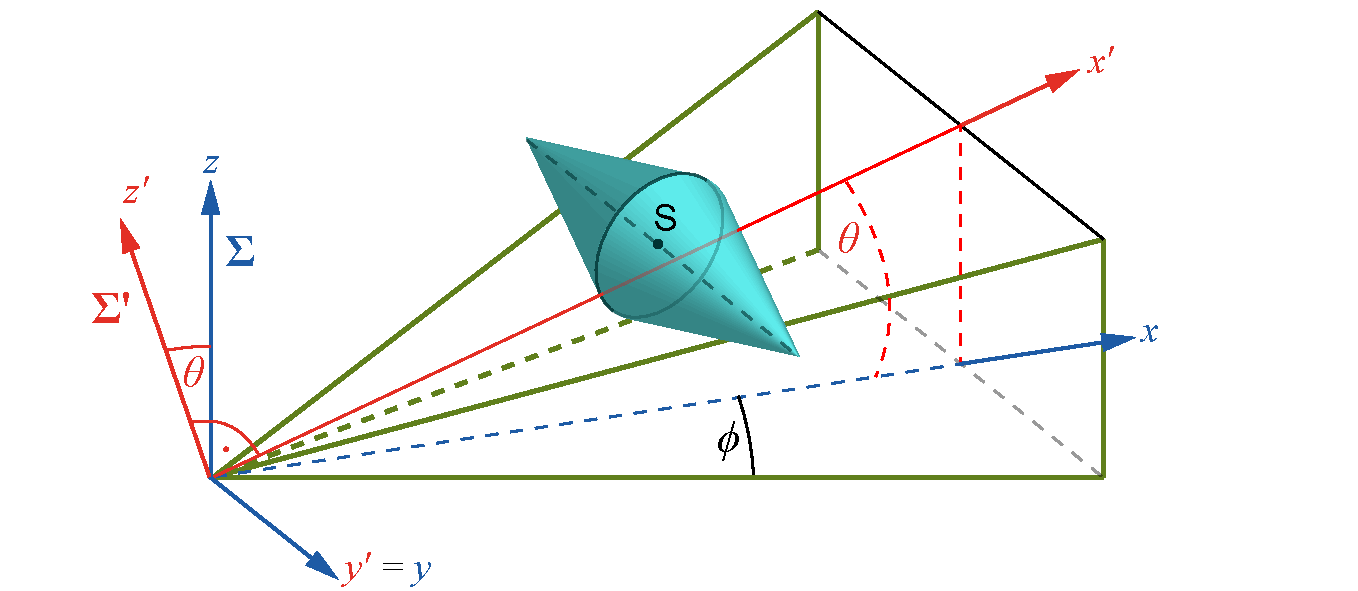
\includegraphics[width=\textwidth]{Doppelkegel01.pdf}
  \caption[Aufbau des aufw�rts laufenden Doppelkegels.]{Aufbau des aufw�rtslaufenden Doppelkegels auf einem Paar von Schienen, die unter einem �ffnungswinkel von $2\phi$ stehen und gegen die horizontale Ebene um einen Winkel $\theta$ geneigt sind. Eingezeichnet sind auch die Koordinatensysteme $\vec{\Sigma}$ und $\vec{\Sigma}'$.} \label{abb:bew_doublecone01}
\end{figure}

\begin{figure}
  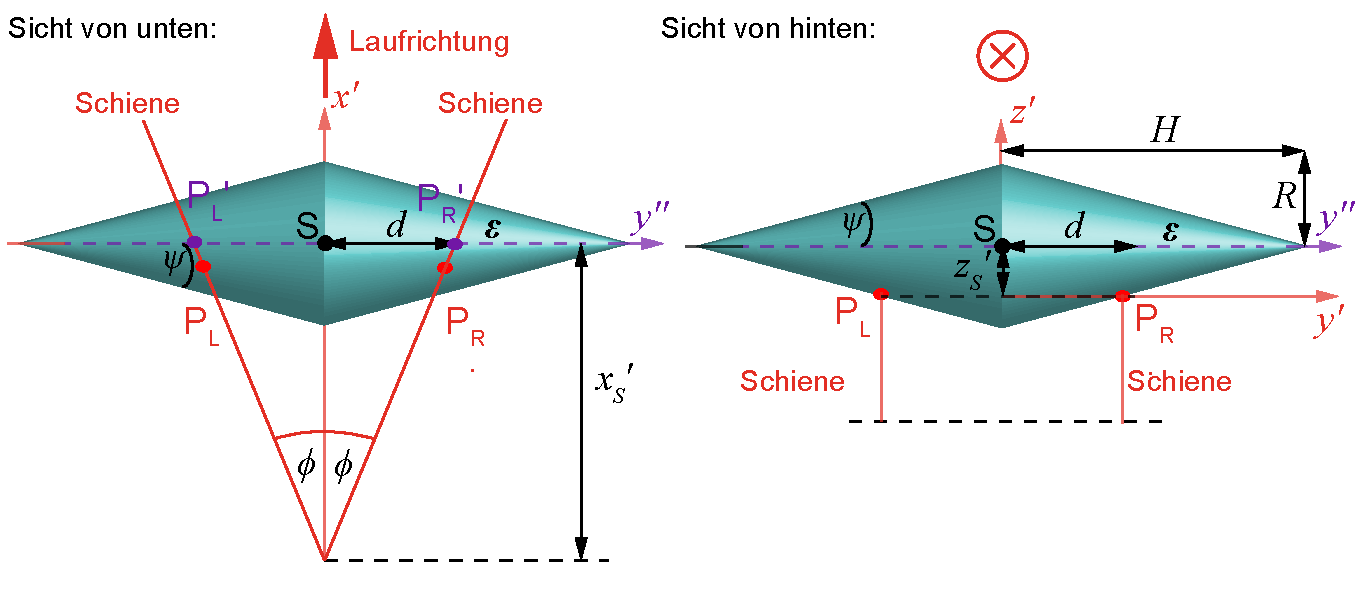
\includegraphics[width=\textwidth]{Doppelkegel02.pdf}
  \caption[Geometrie des aufw�rts laufenden Doppelkegels.]{Geometrie des aufw�rts laufenden Doppelkegels. Man beachte, dass wir zur (vorl�ufigen) Vereinfachung der Rechnung die realen Auflagepunkte $\text{P}_\text{L},~\text{P}_\text{R}$ n�herungsweise unter die Symmetrieachse $\vec{\epsilon}$ in die Punkte $\text{P}_\text{L}',~\text{P}_\text{R}'$ gelegt haben.} \label{abb:bew_doublecone02}
\end{figure}

Man liest aus \figref{bew_doublecone02}, in der das System schiefe Schienen und Doppelkegel im Schnitt von unten und von hinten ebenso wie die verwendeten Koordinatensysteme $\vec{\Sigma}, \vec{\Sigma}'$ dargestellt sind, die folgenden geometrischen Beziehungen f�r die Position des Schwerpunktes S im KOS $\vec{\Sigma}'$ ab:
        \begin{align}
            y_\text{S}' &= \frac{\D}{\tan\phi}\,, ~~~~x_\text{S}' = 0 \,~~~~z_\text{S}' = \lk H-d\rk\,\tan\psi = \lk R\cot\psi-d\rk\,\tan\psi\,,\nonumber \\
	          \rightarrow z_\text{S}' &= R-y_\text{S}'\,\tan\phi\,\tan\psi = - y_\text{S}'\tan\phi\,\tan\psi + H\tan\psi\,. \label{eq:bew_doublecone03} 
        \end{align}

Das ist eine lineare Funktion in $z_\text{S}' = z_\text{S}'(y_\text{S}')$, der Schwerpunkt bewegt sich also interessanterweise auf einer Geraden.
Wir haben bei der Herleitung von \eqref{eq:bew_doublecone03} allerdings die N�herung gemacht, dass der Auflagepunkt des Kegels auf den Schienen (der sogenannte Rollpunkt) direkt unter der Symmetrieachse des Doppelkegels liegt.
Wir werden diese Einschr�nkung sp�ter aufheben.\\ 
Gehen wir nun in das Koordinatensystem $\vec{\Sigma}$, das durch Drehung um den Anstiegswinkel $\theta$ um die gemeinsame $x=x'$-Achse aus $\vec{\Sigma}'$ hervorgeht (\figref{bew_doublecone01}). Wir erhalten\footnote{Da $x_\text{S}= x_\text{S}' = 0$, haben wir effektiv ein zweidimensionales System.}
        \begin{align}
            \begin{pmatrix}
                    y_\text{S} \\
                    z_\text{S}
            \end{pmatrix}
            &=
            \begin{pmatrix}
                    \cos\theta & -\sin\theta \\
                    \sin\theta & \cos\theta
            \end{pmatrix}
            \begin{pmatrix}
                    y_\text{S}' \\
                    z_\text{S}'
            \end{pmatrix}\,,\nonumber \\
            z_\text{S} &= y_\text{S}'\,\sin\theta + z_\text{S}'\,\cos\theta = y_\text{S}'\,\sin\theta +\lk R-y_\text{S}'\,\tan\phi\,\tan\psi\rk\,\cos\theta\,,\nonumber\\
            z_\text{S} &= y_\text{S}'\,\lk \sin\theta-\tan\phi\,\tan\psi\,\cos\theta\rk + R\,\cos\theta\,. \label{eq:bew_doublecone04}
        \end{align}
Wenn der Ausdruck in der Klammer negativ ist, dann wird $z_\text{S}$ mit zunehmendem $y_\text{S}'$ (also beim Aufrollen) kleiner, \dh der Schwerpunkt sinkt.
Eine Bedingung f�r das \glqq Aufw�rtsrollen\grqq{} ist also 
        \begin{align}
            \tan\theta \leq \tan\phi\,\tan\psi \,,\label{eq:bew_doublecone06}
        \end{align}
was eine geometrische Beziehung zwischen den drei Winkeln $\phi$ (halber �ffnungswinkel der Schienen), $\psi$ (halber Kegelwinkel) und $\theta$ (Schienenneigung) ist. 
Beim Aufw�rtsrollen wird also durch Absenken des Schwerpunktes um $\Delta z_\text{S}$
potentielle Energie in kinetische Energie der Translation und der Rotation umgewandelt.
Im Grenzfall, wenn nur noch die Kegelspitzen die Schienen ber�hren ($y_\text{S}'=H/\tan\phi$),
wird der Doppelkegel ausschlie�lich Rotationsenergie besitzen,
sodass wir folgende Energiebilanz aufschreiben k�nnen:
        \begin{align}
        \begin{split}
            \Delta T_\text{Rot} &= -\Delta U \, \rightarrow \frac{1}{2}\,J_\text{S}\,{\omega_\text{f}}^2 = -m\,g\,\Delta z_\text{S,f} \,. \label{eq:bew_doublecone07}
        \end{split}
        \end{align}
In \cite{Gallitto2011} wurden Experimente f�r einen homogenen Doppelkegel mit folgenden Werten angegeben:
        \begin{align*}
          \phi &= \SI{15.5}\degree\,, ~\theta = \SI{6.5}\degree\,, ~ \psi = \SI{24.78}\degree\,, ~ R = \SI{30}{\mm}\,, ~ H = \SI{65}{\mm}\,, ~M = \SI{122.5}{\g}\,.
          %R &= \SI{30}{\mm}\,, ~~~~ H = \SI{65}{\mm}\,, ~~~~ \varrho = \varrho_\text{Al}=\SI{2.7}{\g\per\cm\cubed}\,, ~~~~ M = \SI{122.5}{\g}\,,  ~~~~ ,.
        \end{align*}
F�r das Tr�gheitsmoment bezogen auf die Symmetrieachse des Doppelkegels ermittelt man
$J_\text{S} = \frac{3}{10}\,M\,R^2 = \SI{330.75}{\g\cm\squared}$.
Die finale Rotationsfrequenz $\omega_\text{f}$ ergibt sich
aus der H�hen�nderung $\Delta z_\text{S,f}$, die man aus geometrischen �berlegungen
zu $\Delta z_\text{S,f} \approx \SI{3}{\milli\metre}$ bestimmen kann.
Aus \eqref{eq:bew_doublecone07} folgt, dass die finale Rotationsfrequenz
$\omega_\text{f}$ beim homogenen Doppelkegel in etwa 
        \begin{align*}
            \omega_\text{f} = \sqrt{\frac{20g+\Delta z_\text{S,f}}{3R^2}} &\approx \SI{14.8}{\radian\per\second} \approx 2.3\,\text{Umdrehungen}\,\SI{}{\per\second}
        \end{align*}
betr�gt und interessanterweise nicht von der Masse abh�ngt.

\subparagraph{\textbf{Lagrange-Funktion und Lagrange-Gleichungen des Doppelkegels}}

Wir wollen uns nun der zeitlichen Dynamik zuwenden.
Wir folgen dabei den Betrachtungen in \cite{Gandhi2005}
und wollen den Lagrange-Formalismus benutzen.
Dabei ber�cksichtigen wir jetzt, dass die Kontaktpunkte $\text{P}_\text{L}$
\bzw $\text{P}_\text{R}$ von Schiene und Kegelmantel
nicht in der die Symmetrieachse des Kegels enthaltenden vertikalen Ebene liegen,
sondern vielmehr mit der Symmetrieachse eine Ebene bilden,
die die vertikale Ebene unter einem Winkel schneidet (\figref{bew_doublecone03}).%
\footnote{Die Situation eines rollenden Zylinders auf der V-f�rmigen Doppelschiene
ist anders als die des Doppelkegels.
Man macht sich leicht klar, dass beim Zylinder die Normale von der Rollfl�che
durch den Rollpunkt auch durch die Symmetrieachse $\epsilon$ geht,
nicht jedoch beim Doppelkegel.
Ein Doppelkegel, der auf parallelen Schienen abrollt,
h�tte daher auch dieselbe Abrollsituation wie ein Zylinder.}
Wir m�ssen daher zum Aufstellen der Lagrange-Funktion
die Lage der Kontaktpunkte relativ zum Schwerpunkt kennen. 
In \figref{bew_doublecone03} und \figref{bew_doublecone04} haben wir deshalb
die Geometrie genauer dargestellt, dabei zeigt in \figref{bew_doublecone04}
der Kreis den Querschnitt des Doppelkegels in seiner Schwerpunktebene an.
Die rote Linie ist die Schnittlinie der $x'$-$y'$-Ebene von $\vec{\Sigma}'$ mit einer Ebene,
die senkrecht zur Symmetrieachse des Doppelkegels steht.
$\text{P}$ ist der sogenannte virtuelle Kontaktpunkt.
Es wird sich als vorteilhaft erweisen, dass man zur Berechnung der Rotationsenergie
die Koordinaten des virtuellen Kontaktpunktes $\text{P}$ nutzt.
Es ergeben sich dadurch deutlich einfachere Beziehungen f�r die Rotationsenergie.

\begin{figure}
  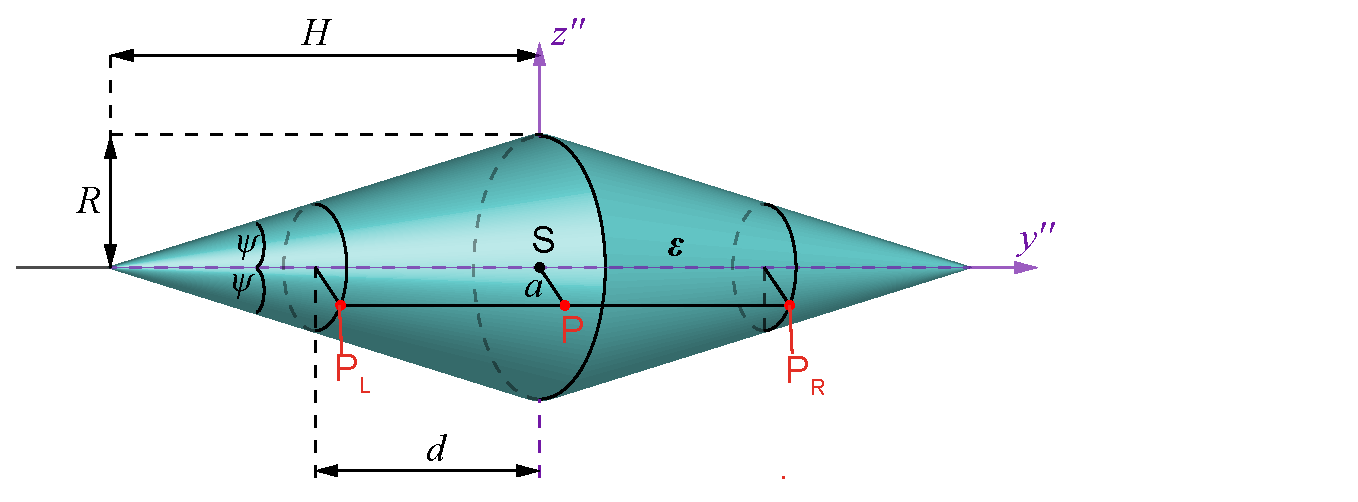
\includegraphics[width=\textwidth]{Doppelkegel03.pdf}
  \caption[Geometrie des Doppelkegels im mitbewegten KOS.]{Geometrie des Doppelkegels im mitbewegten KOS $\vec{\Sigma}''$. $\text{P}_\text{L}, \text{P}_\text{R}$ sind die realen Kontaktpunkte auf den Schienen. $\text{P}$ ist ein \anf{virtueller Kontaktpunkt} im Abstand $a$ vom Schwerpunkt $\text{S}$, $\psi$ ist der halbe �ffnungswinkel der Kegel.} \label{abb:bew_doublecone03}
\end{figure}

Wir werden daher als n�chstes die Koordinaten des Punktes P
als Funktion der Schwerpunktkoordinaten herleiten,
wobei sich der Punkt vom tats�chlichen Kontaktpunkt
nur in seiner $x''$-Koordinate unterscheidet \cite{Gandhi2005}. Daraus wird der
Winkel $\alpha = \alpha_\text{P}$ und die L�nge $a = a_\text{P}$ bestimmt, womit 
der Punkt P eindeutig charakterisiert ist. 
Zun�chst brauchen wir dazu den Normalenvektor $\vec{n}$ an einem Punkt $x'',y'',z''$
auf der Kegeloberfl�che und starten deshalb mit der Kegelgleichung f�r die Oberfl�che

        \begin{align*}
            f\lk x'',y'',z''\rk &= -\sqrt{\lk H-x''\rk^2\,\tan^2\psi -{y''}^2}-z'' = 0 \,,\\
            \vec{n}_\text{K} &= \vec{\nabla}f = \frac{1}{\sqrt{\lk H -x''\rk^2\,\tan^2\psi -{y''}^2}} \,
						\begin{pmatrix}
                    \lk H-x''\rk\,\tan^2\psi\\
                     y''\\
                    -\sqrt{\lk H-d\rk^2\,\tan^2\psi -{y''}^2}
            \end{pmatrix}\,.
        \end{align*}
Speziell f�r den Kontaktpunkt P gilt $y''=y_\text{P}''$ und $y'' = y_\text{P}'' = d$ und somit
        \begin{align}
            \vec{n}_\text{K,P} = \frac{1}{\sqrt{\lk H-d\rk^2\,\tan^2\psi -{y_\text{P}''}^2}}\,\begin{pmatrix}
                    \lk H-d\rk\,\tan^2\psi \\ y_\text{P}'' \\
                    -\sqrt{\lk H-d\rk^2\,\tan^2\psi -{y_\text{P}''}^2}
            \end{pmatrix}\,.
            \label{eq:bew_doublecone08}
        \end{align}
Der in Richtung der (rechten) Schiene zeigende Einheitsvektor ist gegeben durch 
        \begin{align}
            \vec{e}_\text{S} = 
            \begin{pmatrix}
                    \cos\phi\\
                    \sin\phi\\
                    0
            \end{pmatrix} 
            \label{eq:bew_doublecone09}
        \end{align}
und steht wegen der Rollbedingung tangential zur Kegeloberfl�che, \dh es gilt
        \begin{align}
            \vec{n}_\text{K,P}\cdot \vec{e}_\text{S} = 0\,. \label{eq:bew_doublecone10}
        \end{align}
Daraus k�nnen wir sofort $y_\text{P}''$ zu 
        \begin{align}
            y_\text{P}'' = -\lk H-d\rk\,\tan^2\psi\,\tan\phi \label{eq:bew_doublecone11}
        \end{align}
bestimmen. 

\begin{figure}
\begin{minipage}{\textwidth}
\leftfigure{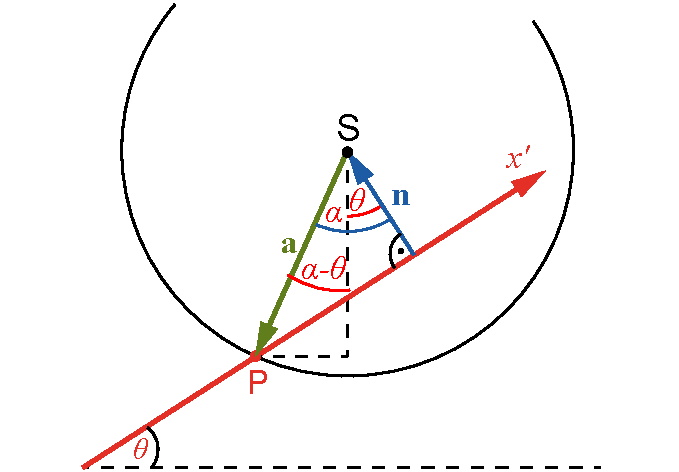
\includegraphics[width=0.5\textwidth]{Doppelkegel04.pdf}}%
\hspace{\fill}
\rightfigure{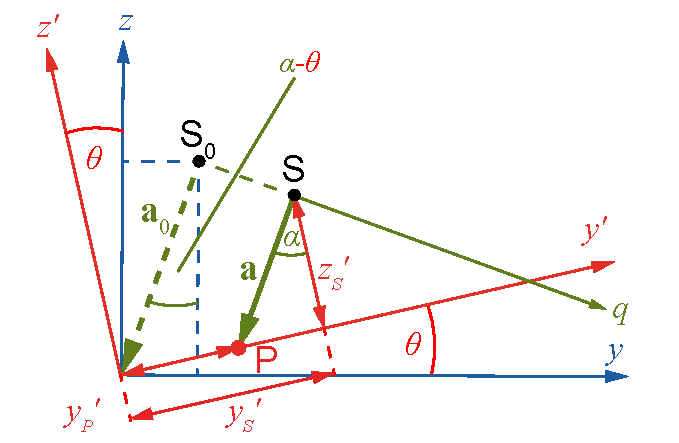
\includegraphics[width=0.5\textwidth]{Doppelkegel05a.pdf}}
\leftcaption[Lage des virtuellen Auflagepunktes beim Doppelkegel.]{Lage des virtuellen Auflagepunktes $\text{P}$ beim aufw�rts rollenden Doppelkegel im KOS $\vec{\Sigma}''$. Der Kreis ist der Querschnitt in der Mittelebene des Doppelkegels.} \label{abb:bew_doublecone04}
\rightcaption[Abstandsvektor und Schwerpunktskoordinaten.]{Beziehung zwischen dem Abstandsvektor $\vec{a}$ und den Schwerpunktskoordinaten ($y_\text{S}', z_\text{S}'$) im KOS $\vec{\Sigma}'$. Definition der generalisierten Koordinate $q$.} \label{abb:bew_doublecone05}
\end{minipage}
\end{figure}

\begin{figure}
  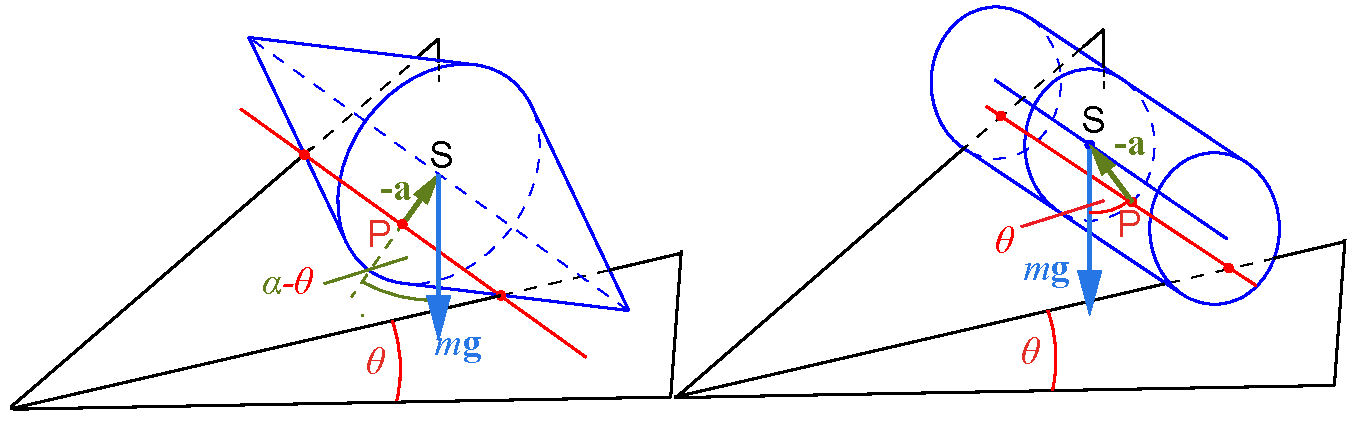
\includegraphics[width=\textwidth]{Doppelkegel04a.pdf}
  \caption[Vergleich der Drehmomente beim Doppelkegel und beim Zylinder.]{Vergleich der Drehmomente beim Doppelkegel und beim Zylinder.} \label{abb:bew_doublecone04a}
\end{figure}


Aus \figref{bew_doublecone04} erhalten wir andererseits
        \begin{align*}
            y_\text{P}'' &= -a\,\sin\alpha\,, 
        \end{align*}
woraus wir schlie�lich die gesuchten Gr��en $a$ und $\alpha$ erhalten:
        \begin{align}
            a= \lk H-d\rk\,\tan\psi ~~~~ \text{und} ~~~~ \sin\alpha = \tan\phi\,\tan\psi \,. \label{eq:bew_doublecone12}
        \end{align}
Der Winkel $\alpha$ ist damit vollst�ndig durch die Geometrie von Kegel und\,(!) Schienen festgelegt und konstant.
Wie man aus \figref{bew_doublecone04} und \figref{bew_doublecone04a}a erkennt, bestimmt der Winkel $\alpha-\theta$ die Gr��e des Drehmoments:
\begin{align}
	\MD = -\vec{a} \times m\vec{g}  = -\lk H-d\rk\,\tan\psi\,m\,g \sin(\alpha-\theta)\, \vecppeX \,. \label{eq:bew_doublecone12a}
\end{align}
Zeigt das Drehmoment in die negative $\vecppeX\,$-Richtung, rollt der Kegel in positive $\vecppeY$-Richtung, also \anf{aufw�rts}. Im Gegensatz dazu zeigt das resultierende Drehmoment beim Zylinder immer in positive Richtung $\vecppeX$, der Zylinder kann nur \anf{abw�rts} rollen (\figref{bew_doublecone04a}b).\\
Mit diesem Wissen k�nnen wir nun an die \anf{Konstruktion} der Lagrange-Funktion gehen. Zun�chst bestimmen wir in einem Koordinatensystem $\vec{\Sigma}'$ die Bewegung des Schwerpunktes als Funktion von $x_\text{P}'$ und $\alpha$. Aus \figref{bew_doublecone04} und \figref{bew_doublecone05} sowie \eqref{eq:bew_doublecone11} finden wir 
        \begin{align}
				    d &= y_\text{P}' \tan\phi\,, ~~ z_\text{S}' = a\,\cos\alpha \,, ~~ a= H\,\tan\psi - y_\text{P}'\,\sin\alpha \,,\nonumber \\
            \rightarrow z_\text{S}' &= \lk H\,\tan\psi - y_\text{P}'\,\sin\alpha\rk\,\cos\alpha\,,\\
						 \rightarrow y_\text{S}' &= y_\text{P}' + a\,\sin\alpha = H\,\tan\psi - y_\text{P}'\,\sin\alpha\,~~\text{und}~~ y_\text{P}' = \frac{y_\text{S}' - H\,\tan\psi\,\sin\alpha}{\cos^2\alpha}\,, \label{eq:bew_doublecone13}
        \end{align}
woraus schlie�lich
        \begin{align}
            z_\text{S}' = C\,y_\text{S}' + D ~~ \text{mit} ~~ C = -\tan\alpha ~~~ \text{und} ~~~ D = H\,\tan\psi\,\lk \cos\alpha-\tan\alpha\,\sin\alpha\rk \label{eq:bew_doublecone14}
        \end{align} 

folgt. Wir erhalten also wie in \eqref{eq:bew_doublecone03} wieder einen linearen Zusammenhang wie zwischen $z_\text{S}'$ und $y_\text{S}'$, allerdings mit einigen Unterschieden. Diese resultieren aus der bei der Herleitung von \eqref{eq:bew_doublecone03} gemachten N�herung bez�glich des Rollpunktes.%
\footnote{F�r kleine Winkel $\alpha, \psi$ geht \eqref{eq:bew_doublecone14} in \eqref{eq:bew_doublecone03} �ber.}
Die Erkl�rung daf�r, dass der Schwerpunkt sich auf einer Geraden bewegt,
ist physikalisch recht einleuchtend.
Da die Bewegung des Doppelkegels aus einer �berlagerten Translation ($\vec{v}_\text{trans,S}$)
und Rotation ($\vec{v}_\text{rot}$) besteht, muss f�r die Rollpunkte
$\text{P}_\text{L},\,\text{P}_\text{R}$ und somit auch P gelten:%
\footnote{Wenn die Translationsgeschwindigkeit gleich dem momentanen Radius zum Kontaktpunkt mal der Winkelgeschwindigkeit ist, dann bleibt der Punkt $P$ in Ruhe, \dh wir haben Rollen ohne Gleiten.}  
	\[\vec{v}_\text{rot}=-\vec{v}_\text{trans,S}\,~~\text{und}~~\vec{a}\,\bot\,\vec{v}_\text{trans,S}\,.
\]
Da der Vektor $\vec{a}$ konstant ist und wegen der Symmetrie $x_\text{S} = 0$ gilt, muss $z_\text{S}(y_\text{S})$ eine Gerade sein.\\

F�r die Lagrange-Funktion f�hren wir nun mit \eqref{eq:bew_doublecone14} eine neue generalisierte Koordinate $q$ ein \cite{Gandhi2005}, die sich aus der Distanz des Schwerpunktes auf seiner Bewegungsgeraden vom Startpunkt $y_\text{S0}'$ ergibt (\figref{bew_doublecone05}):
        \begin{align}
            y_\text{S}' &= y_\text{S0}' + q\,\cos\alpha\,, ~~\text{bzw.}~~ q = \frac{y_\text{S}'-y_\text{S0}'}{\cos\alpha}\label{eq:bew_doublecone15} \\
           \text{mit} ~~ y_\text{S0}' &= a_0\,\sin\alpha = R\,\sin\alpha = H\,\tan\psi\,\sin\alpha = H\,\tan^2\psi\,\tan\phi \nonumber \,.
        \end{align}
Daraus erhalten wir mit \eqref{eq:bew_doublecone13} die einfache Beziehung
        \begin{align}
            a(q) = H\,\tan\psi -q\,\tan\alpha\,. \label{eq:bew_doublecone16}
        \end{align}
        Die Rollbedingung lautet dann
        \begin{align*}
            \omega &= -\frac{\dot{q}}{a\lk q\rk} = -\frac{\dot{q}}{H\,\tan\psi - q\,\tan\alpha}\,.
        \end{align*}
Wir f�hren f�r die numerischen Rechnungen zweckm��ige Abk�rzungen $C_1 \ldots C_3$ f�r konstante Gr��en ein 
        \begin{align*}
  C_1 &= \frac{3R^2}{10\tan^2\alpha}\,,~~~C_2 = -g\,\sin(\alpha-\theta)\,,\\
	C_3 &= H\,\frac{\tan\psi}{\tan\alpha}\,~~ \text{und}~~ p(q) = C_3 - q\,.
        \end{align*}   
und erhalten damit die kinetische Energie f�r den homogenen Doppelkegel in relativ kompakter Form zu
        \begin{align}
            T(q, \dot{q}) &= \frac{1}{2}\,M\,\dot{q}^2+\frac{1}{2}\,J_\text{S}\,\omega^2 = \frac{1}{2}\,\dot{q}^2\,M\,\lk 1+\frac{3R^2}{10}\,\frac{1}{\lk H\,\tan\psi -q\,\tan\alpha\rk^2}\rk  \nonumber \\
						&= M\,\frac{1}{2}\,\dot{q}^2\,\lk 1+\frac{C_1}{\lk C_3 - q\rk^2}\rk\,. \label{eq:bew_doublecone17}
	\end{align}
F�r die potentielle Energie m�ssen wir wieder in das $\vec{\Sigma}$ -KOS gehen und erhalten (siehe auch \figref{bew_doublecone04})
        \begin{align}
            U = -m\,g\,q\,\sin\lk\alpha-\theta\rk = m\,C_2\,q\,. \label{eq:bew_doublecone18}
        \end{align}
Hieraus leitet sich wieder die Bedingung f�r das Aufw�rtsrollen ab, n�mlich 
        \begin{align}
            \sin\lk\alpha-\theta\rk &> 0 ~~\Leftrightarrow~~\sin\alpha\,\cos\theta -\cos\alpha\,\sin\theta > 0 ~~\text{\bzw} \nonumber \\
						\tan\theta &< \frac{\tan\phi\,\tan\psi}{\sqrt{1-\tan^2\phi\,\tan^2\psi}}\,. \label{eq:bew_doubleconeCondition}
        \end{align}
Dies geht f�r kleine Winkel, bei denen die Kontaktpunkte nahezu unter der Symmetrieachse liegen,
wieder in die bereits bekannte N�herung \eqref{eq:bew_doublecone06} �ber. 
Man k�nnte beim Blick auf \eqref{eq:bew_doublecone17} vermuten,
dass $T(q, \dot{q})$ f�r $q \rightarrow C_3 = H\,\tan\psi/\tan\alpha $ divergiert.
Das ist aber nicht der Fall, da auch $\lim\limits_{q \to C_3} \dot{q} = 0$ gilt,
wie man leicht �berpr�fen kann. \\
Aus der durch $m$ dividierten Lagrange-Funktion $\hat{\mathcal{L}} = (T-U)/m$ folgt die Bewegungsgleichung f�r $q$,
	\begin{align}
  \ddot{q} & = -\frac{C_1}{p(q)\,(p(q)^2+C_1)}\, \dot{q}^2 - \frac{C_2\,p(q)^2}{p(q)^2+C_1}\,, \label{eq:bew_doubleconeLGL}
	\end{align}
die eine nichtlineare Gleichung darstellt, die wir mit \odevf{} in MATLAB numerisch integrieren. 
% Eventuell Darstellung der Nebenrechnung
%\begin{nebenrechnung}{Nebenrechnung:}
%\begin{align*}
    %\hat{\mathcal{L}} = \frac{\mathcal{L}}{M} = \underbrace{ \frac{1}{2}\,\dot{q}^2\,\lek 1+ \frac{C_1}{\lk C_3-q\rk^2}\rek}_{\substack{T}}  - 
%\underbrace{C_2\,q }_{\substack{U}}
%\end{align*}
%\begin{align*}
    %\frac{\D}{\D t}\, \frac{\d \hat{\mathcal{L}}}{\d \dot{q}} &= \ddot{q}\, \underbrace{\lek 1 + \frac{C_1}{\lk C_3-q\rk^2}\rek}_{Q} + \dot{q}\,\frac{\D}{\D t}\,\frac{C_1}{\lk C_3-q\rk^2} 
    %= \ddot{q}\,Q + \frac{2C_1}{\lk C_3-q\rk^3}\,\dot{q}^2 \\
    %\frac{\d \hat{\mathcal{L}}}{\d q} &= \frac{1}{2}\,\dot{q}^2\,\frac{C_1\,\lk -2\rk\lk -1\rk}{\lk C_3-q\rk^3}+C_2 = \frac{C_1}{\lk C_3-q\rk^3}\,\dot{q}^2-C_2 \\
    %0 & = \frac{\d }{\d t}\, \frac{\d \hat{\mathcal{L}}}{\d \dot{q}} -  \frac{\d \hat{\mathcal{L}}}{\d q} = \ddot{q}\,Q + \frac{2C_1}{\lk C_3-q\rk^3}\,\dot{q}^2 - \frac{C_1}{\lk C_3-q\rk^3}\,\dot{q}^2 +C_2 \\
 %C_3-q &= p ~~~\rightarrow ~~  0 = \frac{p^2 + C_1}{p^2}\,\ddot{q} + \frac{C_1}{p^3}\,\dot{q}^2 + C_2 
%\end{align*}
%\end{nebenrechnung}
Alternativ zur Lagrange-Gleichung kann man nat�rlich auch unter Ber�cksichtigung der Energieerhaltung aus \eqref{eq:bew_doublecone17} und \eqref{eq:bew_doublecone18} mit $E_0 = T + U = U(q_0)$ die Variable $\dot{q}$ als Funktion von $q$ darstellen,
	\begin{align}
		\dot{q}= \pm \sqrt{\frac{2\lk E_0 + m\, g\, \sin(\alpha-\theta) \rk}{m+ J_\text{S}/\lk H\,\tan\psi - q\,\tan\alpha \rk^2}} = F(q)\,, \label{eq:bew_doublecone20}
	\end{align}
und somit $\dot{q}=\dot{q}(q) = \dot{q}(y)$ berechnen. Wie man an \eqref{eq:bew_doublecone20} erkennt, ist $\lim\limits_{q \to C_3} \dot{q} = 0$, was unsere Aussage best�tigt, dass zum Ende der Bewegung keine Translationsenergie mehr vorhanden ist (vgl.\ \figref{bew_doublecone06}). �ber Trennung der Variablen erhalten wir aus \eqref{eq:bew_doublecone20}
	\begin{align}
			t + C = \int\limits_{0}^{t} \D\,t' =  \int\limits_{0}^{q} F(q') \D\,q' \,. \label{eq:bew_doublecone21}
	\end{align}
Dieses Integral ist ebenfalls numerisch l�sbar und wir erhalten die inverse Funktion $t(q)$, aus der wir die gesuchte Funktion $q(t)$ bestimmen k�nnen.\\
Das Ergebnis $\dot{q}(q)$, sowie $T_\text{Trans}\lk q\rk$ und $T_\text{Rot}\lk q\rk$ \bzw $f_\text{pot}\lk q\rk$ sind in \figref{bew_doublecone06} zu sehen
(siehe \mscre \mlbewref{Doppelkegel01.m} bis \mlbewref{Doppelkegel04.m}).
�ber \eqref{eq:bew_doublecone15} ist $q$ mit $y_\text{S}'$ und $y_\text{S}'$ wiederum �ber \eqref{eq:bew_doublecone03} mit $y_\text{S}$ verkn�pft.
Diese messbaren Gr��en sind als $z_\text{S}(y_\text{S})$ \bzw $y_\text{S}(t)$ und $z_\text{S}(t)$ in \figref{bew_doublecone07} dargestellt.

\begin{figure}
  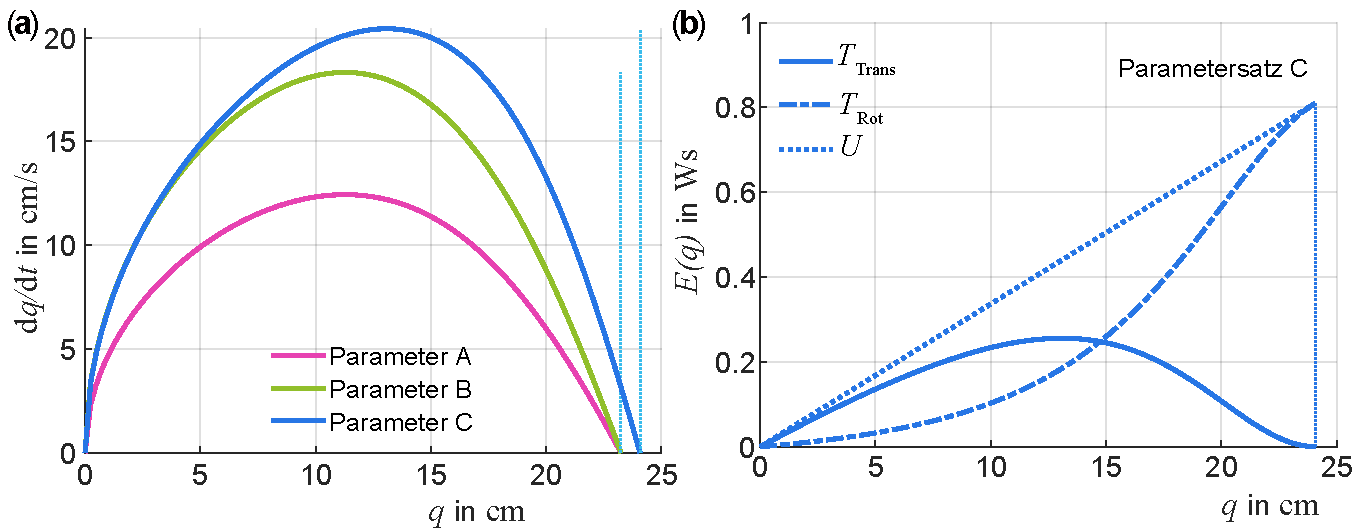
\includegraphics[width=\textwidth]{Doppelkegel06.pdf}
  \caption[Phasenraum und Energieanteile des aufw�rts laufenden Doppelkegels.]{\fa Phasenraum und \fb Energieanteile des aufw�rts laufenden Doppelkegels als Funktion der generalisierten Koordinate $q$. Parameter A: $\phi=15.5\degree,\, \theta=6.5\degree\,, J=\SI{330.75}{\g\cm\squared}$,\, B: $\phi=15.5\degree,\, \theta=5.5\degree,\, J=\SI{330.75}{\g\cm\squared}$,\,  C: $\phi=15.0\degree,\, \theta=5.5\degree,\, J=\SI{165.75}{\g\cm\squared}$. Sonstige Parameter: $H=\SI{6.5}{\cm},\, \psi=24.8\degree,\, M=\SI{122.5}{\g}$. Siehe auch \mscr{} \mlbewref{Doppelkegel04.m}.} \label{abb:bew_doublecone06}
\end{figure}

\begin{figure}
  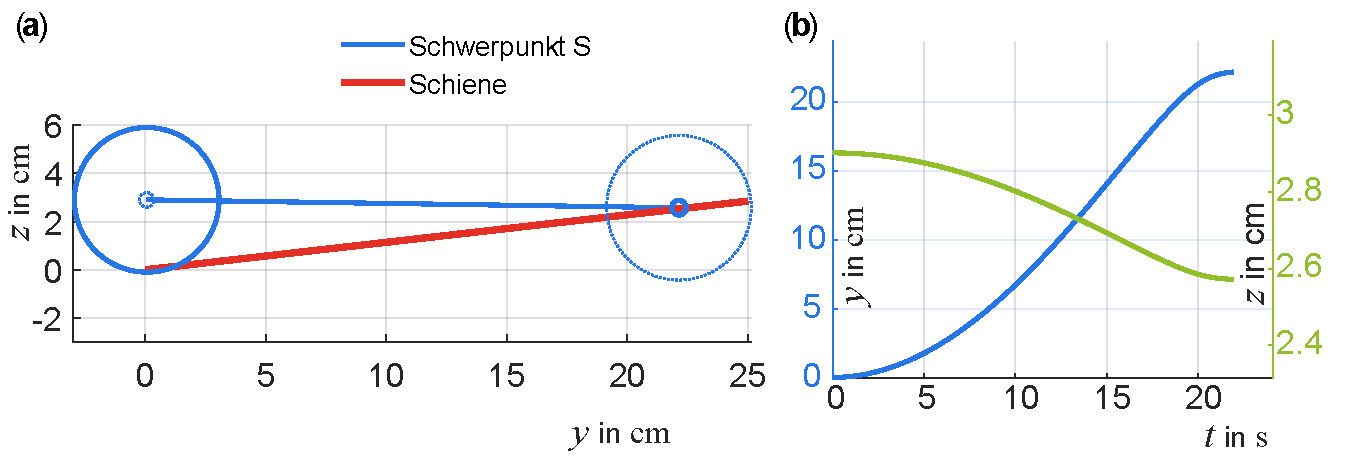
\includegraphics[width=\textwidth]{Doppelkegel07.pdf}
  \caption[Dynamik des aufw�rts laufenden Doppelkegels.]{Dynamik des aufw�rts laufenden Doppelkegels in kartesischen Koordinaten $y, z$. Siehe auch \mscr{} \mlbewref{Doppelkegel02.m}.} \label{abb:bew_doublecone07}
\end{figure}

Wir wollen noch darauf hinweisen, dass sich in der Literatur an verschiedenen Stellen leicht andere Formeln finden, die im Allgemeinen aus der unterschiedlichen Definition des Rollpunktes resultieren. In \probref{bew_doubleconecomp} vergleichen wir die Ergebnisse der verschiedenen Ans�tze miteinander.

\newpage

\subsubsection{Stabilit�t von Schienenfahrzeugen mit starren Achsen} \label{kap:bew_traintracks} 

Die im vorgehenden Kapitel behandelte Physik des Doppelkegels
hat eine ganz konkrete Anwendung in der Eisenbahntechnik gefunden.
Wer sich die Eisenbahnr�der genau anschaut (\figref{bew_TrainWheel01}), wird erkennen,
dass das Profil der R�der einem Ausschnitt aus einem Doppelkegel �hnelt.
Dieses Profil hat einen positiven Einfluss auf die Stabilit�t von Schienenfahrzeugen
entlang der Bewegung eines Gleises, bei der es stets zu unvermeidbaren lateralen St�rungen kommt.
Die Frage nach der Stabilit�t von Z�gen auf Gleisen mag nicht offensichtlich erscheinen. Vielfach h�rt man die falsche Erkl�rung, dass die erstaunliche Stabilit�t
eines kilometerlangen Zuges, der auf einem nur $\SI{1435}{\mm}$ breiten Gleis f�hrt,
durch den Radkranz/Flansch (\figref{bew_TrainWheel01} und \figref{bew_TrainWheel02}) zustandekommt. M�glicherweise brachte seshalb sogar Feynman\footnote{Richard Feynman (1918--1988) war ein US-amerikanischer Physiker und gilt als einer der gro�en Physiker des 20.\ Jahrhunderts, der wesentliche Beitr�ge zum Verst�ndnis der Quantentheorie geliefert hat. 1965  erhielt er 1965 den Nobelpreis f�r seine Arbeiten zur Quantenelektrodynamik. Feynman war es �beraus wichtig, die Gesetzm��igkeiten der Physik anschaulich und verst�ndlich Studenten und auch Laien nahezubringen.}\indexp{Feynman, Richard} das Thema in den 1970er Jahren (\url{https://www.youtube.com/watch?v=y7h4OtFDnYE}) in die popul�re Physik ein.
Tats�chlich zeigt die genauere Betrachtung, dass bei Rad-Schiene-Systemen
mit starr gekoppelten Achsen konisch profilierte R�der benutzt werden.
Da bei einem solchen Radsatz \zb bei Kurvenfahrten die Rollradien der beiden R�der
unterschiedlich gro� sind, die R�der sich aber gleich schnell drehen,
vollf�hrt das Rad mit dem gr��eren Rollradius einen l�ngeren Weg nach vorne
als das Rad mit dem kleineren Rollradius.
Daher lenkt ein zu weit links stehender Radsatz nach rechts und umgekehrt.
Hierdurch kommt es zu einer Art Schlingerbewegung, die wir
mit einer (r�umlichen) Differentialgleichung beschreiben k�nnen.
Im Grenzfall kleiner Abweichungen (Linearisierung) erh�lt man die in \figref{bew_TrainWheel03} dargestellte Sinuskurve, 
die erstmalig 1883 von Johannes Klingel\footnote{Johannes Klingel war ein Baurat und Ingenieur, der \ua an der Polytechnischen Hochschule Karlsruhe wirkte.}\indexp{Klingel, Johannes} an der damaligen Hochschule Karlsruhe ver�ffentlicht wurde.
Wir wollen in diesem Kapitel diese sogenannte Klingel-Formel herleiten
und brauchen die dabei wirkenden Kr�fte zun�chst nicht zu ber�cksichtigen,
sondern leiten den Sinuslauf aus einfachen geometrisch-kinematischen �berlegungen ab. 
Wir betrachten dazu \figref{bew_TrainWheel04}, die den Radk�rper schematisch als Doppelkegel von hinten zeigt und zwar in Normallage (gelb) und durch eine seitliche St�rung leicht nach links verschoben (blau).

\begin{figure}
\begin{minipage}{\textwidth}
\leftfigure{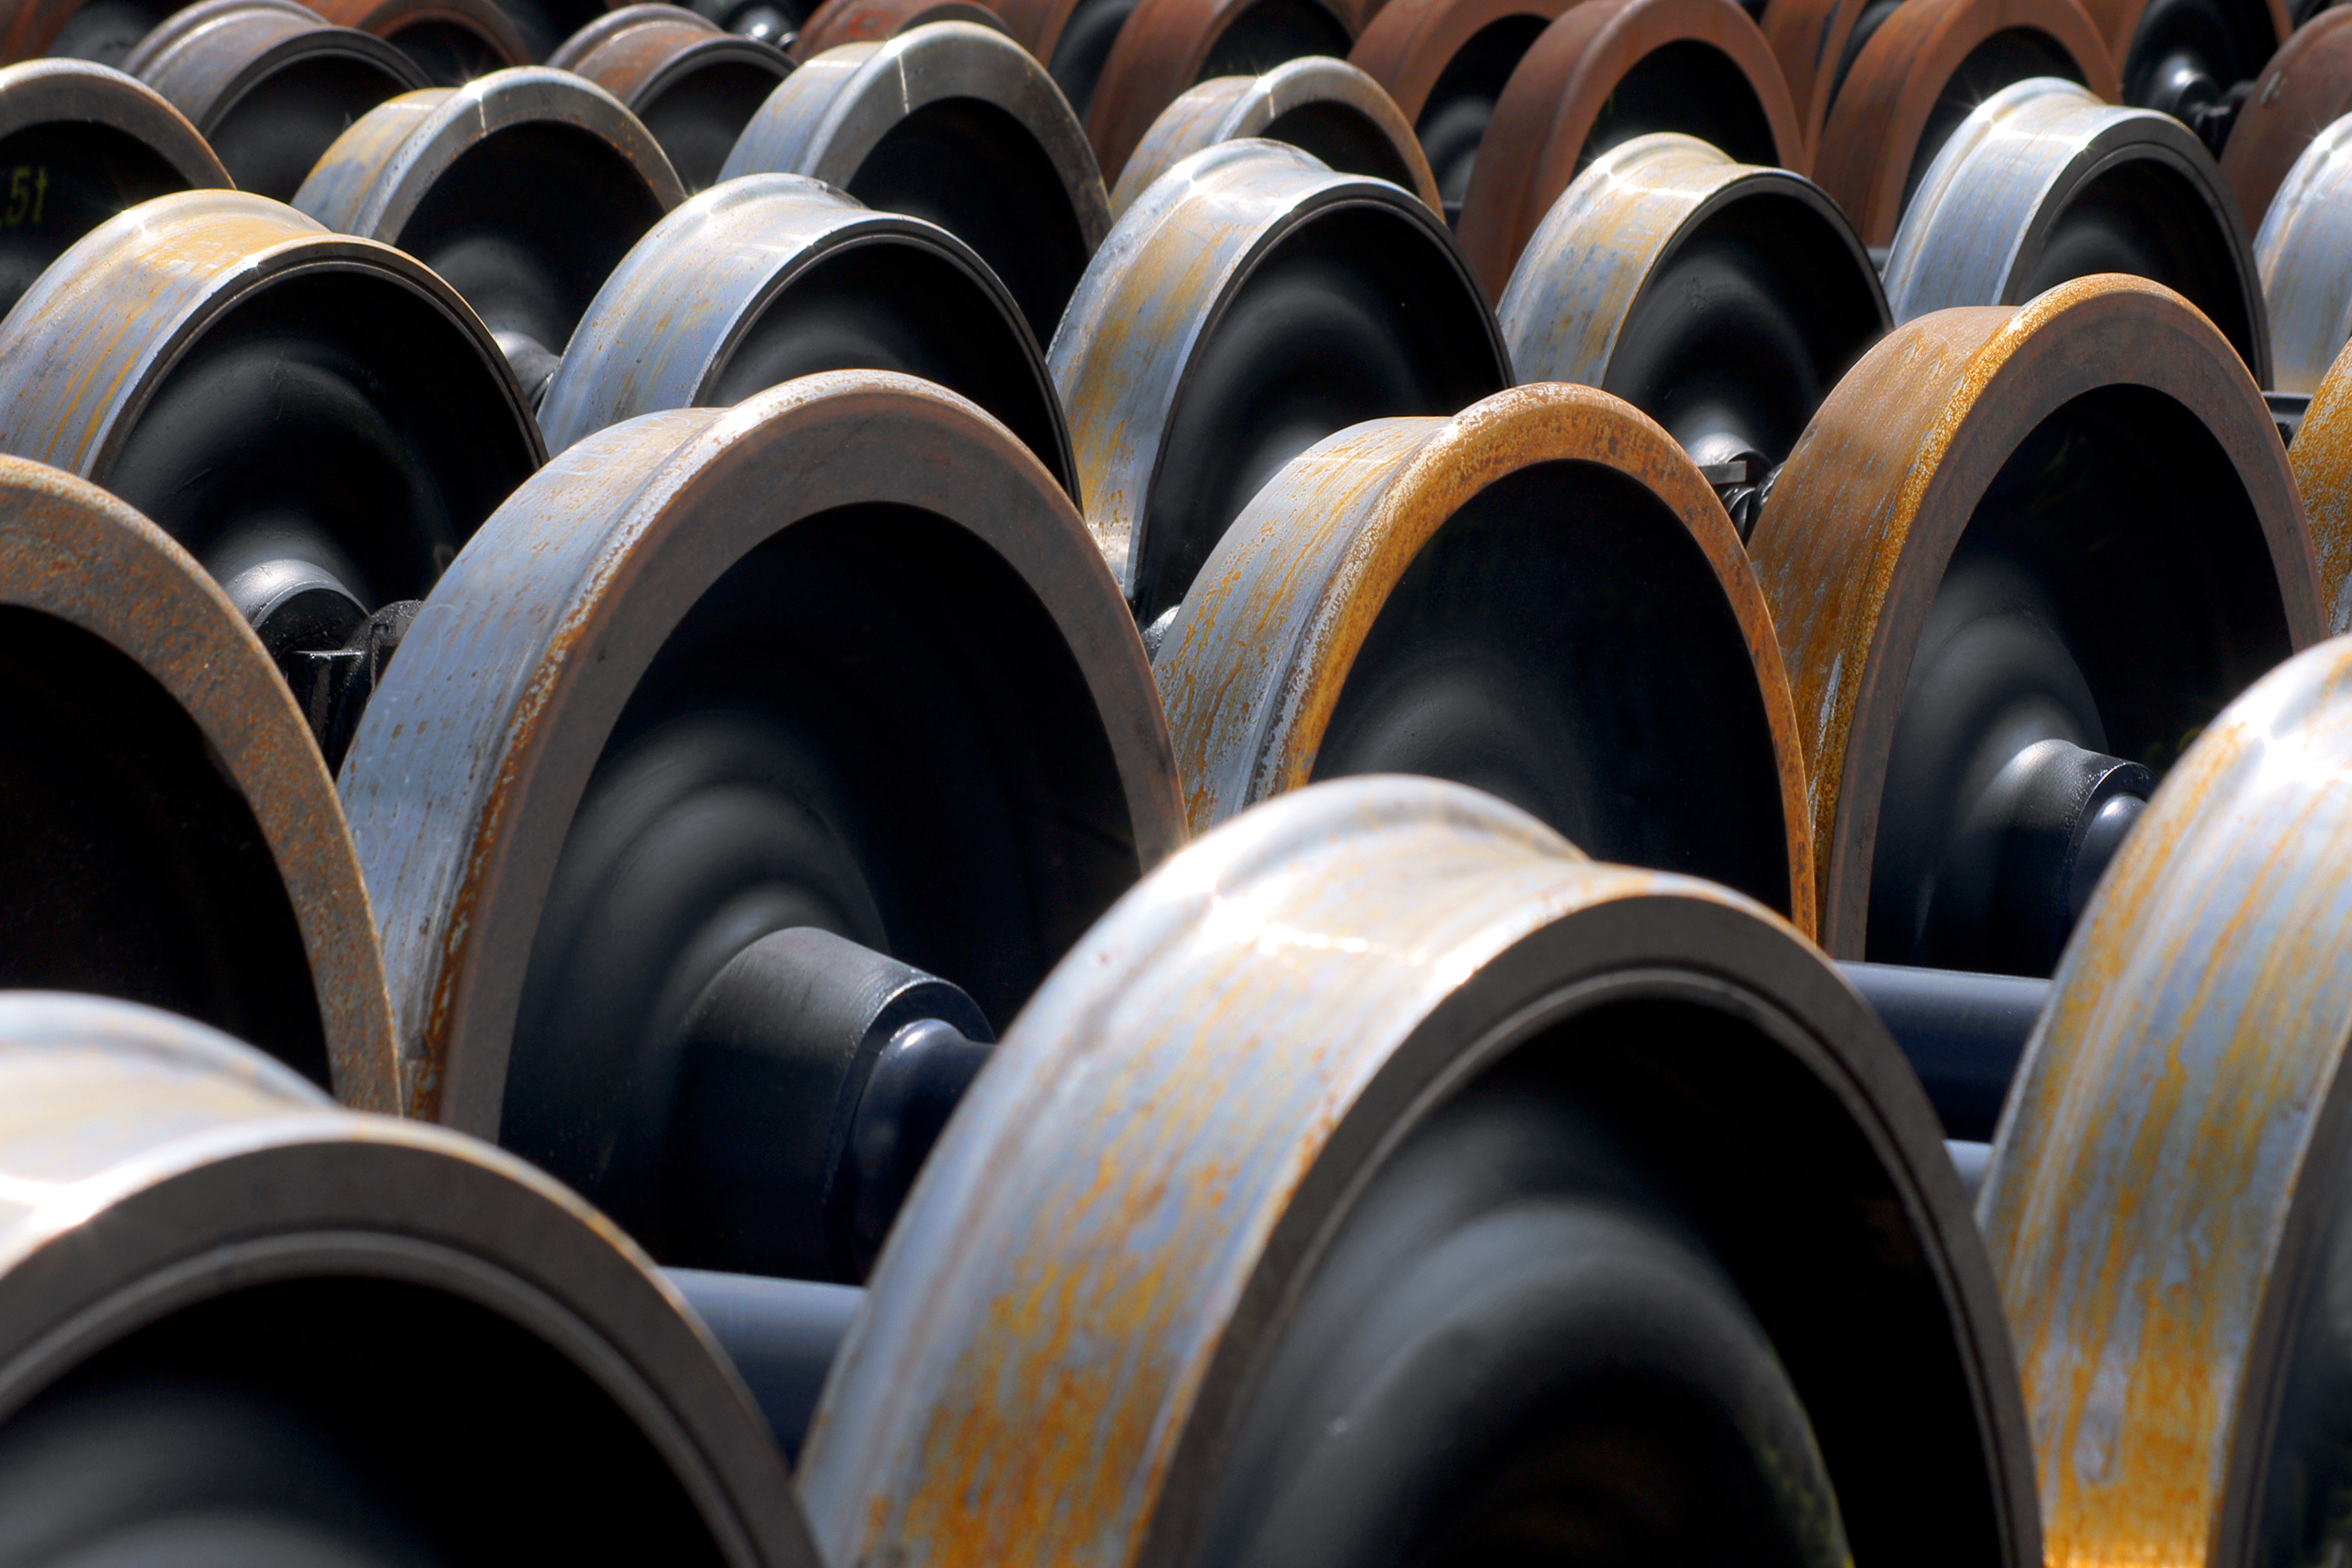
\includegraphics[width=0.4\textwidth]{TrainWheel.jpeg}}%
\hspace{\fill}
\rightfigure{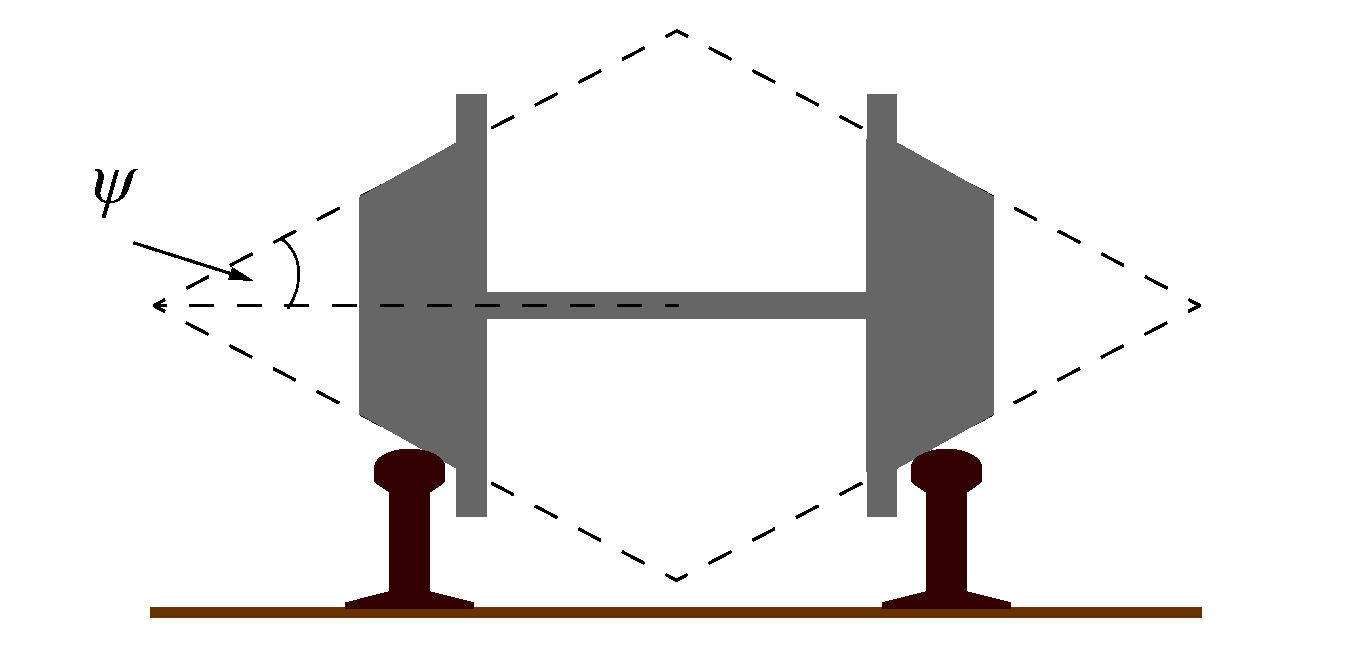
\includegraphics[width=0.6\textwidth]{WaggonAchse.pdf}}
\leftcaption{Eisenbahnr�der.} \label{abb:bew_TrainWheel01}
\rightcaption[Schematische Darstellung eines Eisenbahnachse auf einer Schiene.]{Schematische Darstellung eines Eisenbahnachse auf einer Schiene durch einen Doppelkegel. Der Winkel $\psi$ ist stark �berh�ht gezeichnet. In der Realit�t betr�gt er weniger als $0.05\,\text{rad} \approx 2.865\degree$.}\label{abb:bew_TrainWheel02}
\end{minipage}
\end{figure}

\begin{figure}
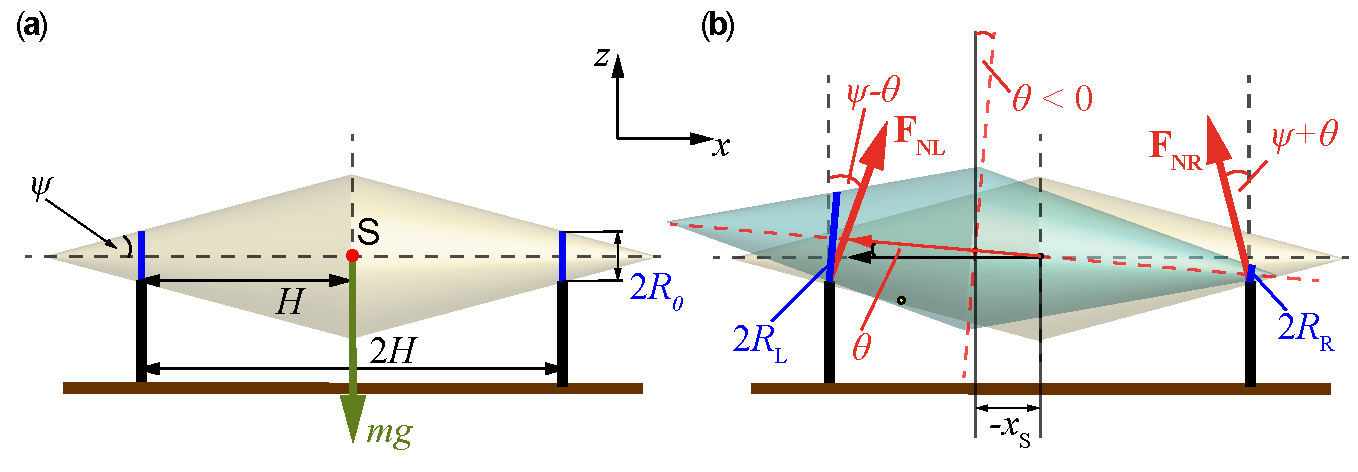
\includegraphics[width=\textwidth]{LateraleStoerung.pdf}%
\caption[Laterale St�rungen auf eine Radachse auf einer Doppelschiene.]{Laterale St�rungen auf eine Radachse auf einer Doppelschiene (Modellansicht von hinten in Fahrtrichtung). \fa Normallage der Radachse, $2H$ ist die Spurbreite, $\psi$ die Konizit�t der Radform, $R_0$ ist der Rollradius in der Normallage und S der Schwerpunkt der Achse, $m$ die Gesamtmasse von Achse und Achslast. \fb Lage bei lateraler St�rung und wirkende Normalkr�fte. $x_\text{S}$ ist die laterale Verschiebung des Schwerpunktes, $\theta$ der resultierende Kippwinkel aufgrund der Konizit�t, $\vec{F}_\text{N}$ die von der Schienenauflage ausgehenden Normalkr�fte und $R_\text{L}, R_\text{R}$ die neuen resultierenden Rollradien auf dem linken \bzw rechten Auflagepunkt. Der Winkel $\theta$ ist im eingezeichneten Fall negativ.} \label{abb:bew_TrainWheel04}
\end{figure}

    Wir starten von \figref{bew_TrainTrack01}. Als Parameter haben wir den Rollradius $R$, den Radstand $2H$ und die Konizit�t $\psi$. In der Normallage ist der Rollradius $R_0$ durch 
    \begin{align}
        R_0\,\omega_0 = v_0 \,\label{eq:bew_TrainTrack01}
    \end{align}
    mit der Vorw�rtsgeschwindigkeit $v_0$ des Schwerpunktes verbunden, $\omega_0$ ist die Rotationsgeschwindigkeit der Radachse. F�r den lateralen Versatz gilt entsprechend:
    \begin{align}
    \begin{split}
        R_\text{L}\,\omega_0 &= v_\text{L} \,,\\
        R_\text{R}\,\omega_0 &= v_\text{R} \,. 
    \end{split}\label{eq:bew_TrainTrack02}
    \end{align}
%
\begin{figure}
  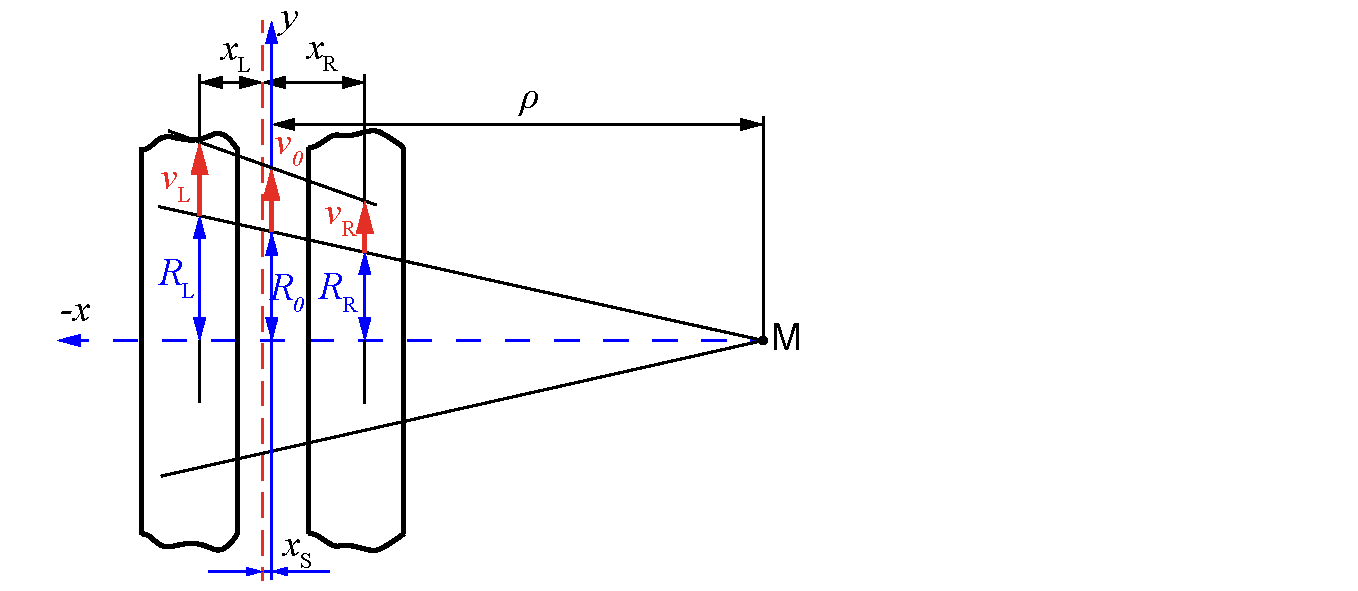
\includegraphics[width=\textwidth]{TrainTrack01.pdf}
  \caption[Kinematische Ableitung der Klingel-Formel.]{Kinematische Ableitung der Klingel-Formel.} \label{abb:bew_TrainTrack01}
\end{figure}
%
    �ber den Strahlensatz l�sst sich aus \figref{bew_TrainTrack01} \bzw \figref{bew_TrainWheel04} direkt ablesen:
    \begin{align}
        \frac{R_0}{\rho\lk x_\text{S} \rk} = \frac{R_\text{L}\lk x_\text{S}\rk - R_\text{R}\lk x_\text{S}\rk}{x_\text{L} + x_\text{R}} \,. \label{eq:bew_TrainTrack03}
    \end{align}
    Wir brauchen also die Differenz der Rollradien und die Gr��e $x_\text{L} + x_\text{R}$. Aus \figref{bew_TrainTrack01} kann man ableiten:
    \begin{align*}
        R_\text{L}-R_0 &\approx x_\text{S}\,\tan\psi\,, \\
        R_\text{R} - R_0 &\approx -x_\text{S}\,\tan\psi 
    \end{align*}
    und
    \begin{align*}
        x_\text{L} + x_\text{R} &\approx 2H\,.
    \end{align*}
    Damit ergibt sich, wenn man mit $\rho \lk x_\text{S} \rk$ als Kr�mmungsradius der Achsenlage ($y$ ist die Fahrtrichtung, $x$ die laterale Dimension) die Beziehung $1/\rho \lk x \rk \approx -\D^2 x_\text{S} / \D y^2$ in \eqref{eq:bew_TrainTrack03} einsetzt:
    \begin{align}
        \frac{\D^2x_\text{S}}{\D y^2} + \frac{\Delta R\lk x\rk}{R_0\,\lk x_\text{L}+ x_\text{R}\rk} = 0\,. \label{eq:bew_TrainTrack04}
    \end{align}
    Das ist schon die Klingel-Formel in ihrer allgemeinen Form (mit Annahme kleiner Winkel und Verschiebungen).\\
    F�r die konische Radform (Doppelkegel-Modell) k�nnen wir die Funktionen $\Delta R\lk x\rk = R_\text{L} -R_\text{R}$ und $\Delta x = x_\text{L} + x_\text{R}$ aufschreiben. %
    Aus \figref{bew_TrainTrack01} kann man ablesen:
    \begin{align}
    \begin{split}
        \left.\begin{aligned}
    	R_\text{L} &\approx R_0 + x_\text{S}\,\tan\psi\\
	    R_\text{R} &\approx R_0 - x_\text{S}\,\tan\psi
	        \end{aligned}
	\right\}
    \quad R_\text{L} - R_\text{R} \approx 2x_\text{S}\,\tan\psi
    \end{split}  \label{eq:bew_TrainTrack05}
    \end{align}
    und 
    \begin{align*}
        x_\text{L} + x_\text{R} &\approx 2H\,.
    \end{align*}
    Damit ergibt sich im Fall des Doppelkegel-Modells f�r die Klingel-Formel
    \begin{align}
        \frac{\D^2x_\text{S}}{\D y^2} +\frac{\psi}{R_0\,H} x_\text{S} = 0  \label{eq:bew_TrainTrack06}
    \end{align}
    und daraus die Wellenl�nge und Frequenz des Sinuslaufs zu 
    \begin{align}
    \begin{split}
        \Lambda_\text{K} &= 2\pi\,\sqrt{\frac{H\,R_0}{\psi}} \,, ~~~ f_\text{K} = \frac{v_0}{2\pi}\,\sqrt{\frac{\psi}{H\,R_0}}\,.
    \end{split} \label{eq:bew_TrainTrack07}
    \end{align}
		Die Gr��e $f_\text{K}$, manchmal auch Klingel-Frequenz genannt, charakterisiert also den sogenannten Sinuslauf (oder Wellenlauf) \cite{Knothe2003}. Die Bewegung ist bei kleinen Amplituden sinusf�rmig und hat eine konstante Wellenl�nge, daher also eine mit der Fahrgeschwindigkeit zunehmende Frequenz (\figref{bew_TrainWheel03a}).

\begin{figure}
  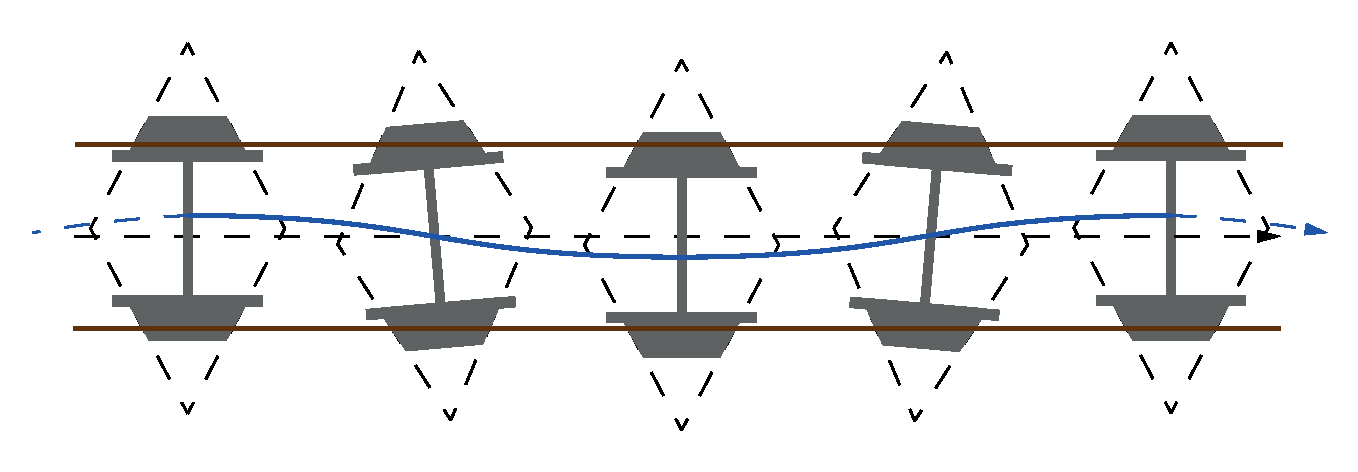
\includegraphics[width=\textwidth]{SinusLauf.pdf}
  \caption[Sinuslauf bei Z�gen mit starrer Achse.]{Sinuslauf bei Z�gen mit starrer Achse (Sicht von oben).} \label{abb:bew_TrainWheel03}
\end{figure}

\begin{figure}
  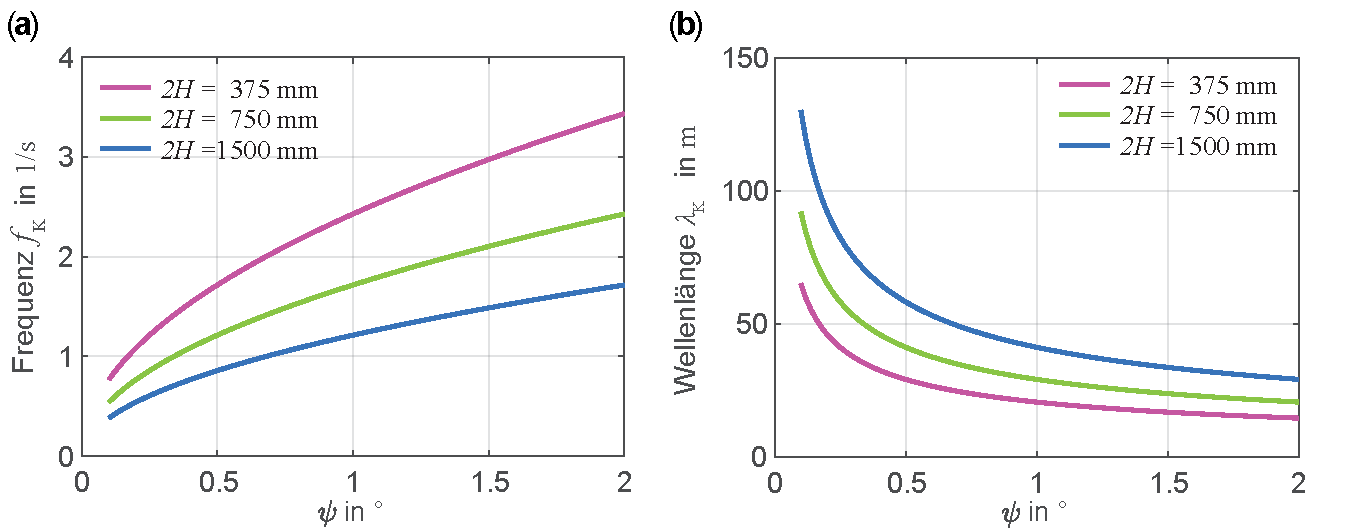
\includegraphics[width=\textwidth]{KlingelFrequenz.pdf}
  \caption[Frequenz und Wellenl�nge des Sinuslaufs als Funktion der Konizit�t.]{\fa Frequenz und \fb Wellenl�nge des Sinuslaufs als Funktion der Konizit�t. Vorw�rtsgeschwindigkeit $v_0 = \SI{50}{\metre\per\second}$.} \label{abb:bew_TrainWheel03a}
\end{figure}

In \probref{bew_TrainTrack} wollen wir uns das Rad-Schiene-System bei lateralen St�rungen dynamisch anschauen und uns auch den Fall anschauen, der eintritt, wenn das System \zb durch einen Lenkfehler gest�rt wird. Wir werden dazu die Reibung ber�cksichtigen und k�nnen dann zeigen, dass mit diesem R�der-Konstruktionsprinzip auch bei Lenkfehlern, also gr��eren lateralen St�rungen, das Schienenfahrzeug stabil bleibt. %Wir folgen dabei der Darstellung in \cite{Shayak2017}.

\newpage
\subsubsection{Der Gyrotwister (\textit{Dynabee})} \index{Gyrotwister}\index{Dynabee} \label{kap:bew_dynabee}

Hinter den verschiedenen kommerziell verwendeten Namen Gyrotwister (Gyro-Twister), Dynabee und Powerball (\figref{bew_GyrotwAufbau}) verbirgt sich ein
Spielzeug, mit dem man Kraft im Arm und die Geschicklichkeit der Bewegung
der Hand �ben kann. Es besteht aus einem (meist kugelf�rmigen) Kreisel, der
in einer Nut eines ebenfalls kugelf�rmigen Geh�uses gef�hrt wird (\figref{bew_GyrotwAufbau2}).\footnote{Meist hat das Geh�use eine kleine kreisf�rmige �ffnung um die Achse senkrecht zur Nut. Diese kann genutzt werden, um den Kreisel z.\,B. durch Abziehen mit einer
Schnur schnell zu beschleunigen. }

\begin{figure}
  \includegraphics[width=\textwidth]{GyrotwAufbau.pdf}
  \caption[Aufbau eines Gyrotwisters.]{Aufbau des Gyrotwisters. \fa US Patent 3726146 (1971) und \fb kommerzielle Ausf�hrung. }
  \label{abb:bew_GyrotwAufbau}
\end{figure}

\begin{figure}
  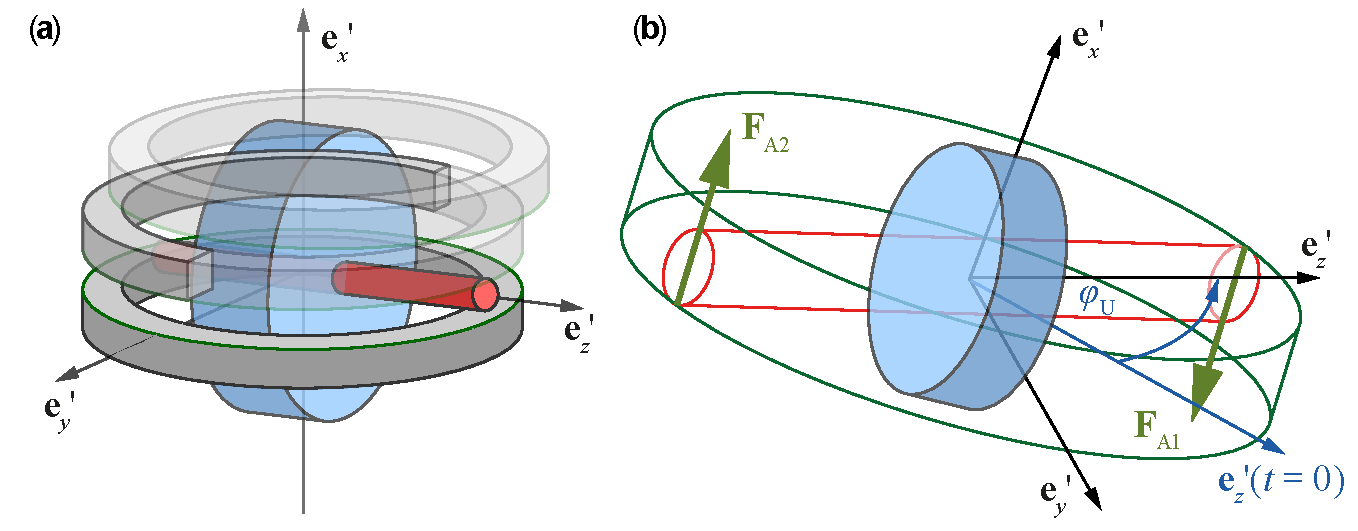
\includegraphics[width=\textwidth]{GyrotwAufbau2.pdf}
  \caption[Geometrie des Kreisels im Gyrotwister.]{Geometrie des Kreisels im
    Gyrotwister: \fa Ein symmetrischer Kreisel wird in einer Nut einer �u�eren
    Halterung gef�hrt. In der Realit�t ist sowohl der Kreisel als auch die
    Halterung nahezu kugelf�rmig.
    \fb Schematische Ausschnittszeichnung mit F�hrungsnut und Achse des Kreisels.
    Achtung: Das eingezeichnete KOS $\tilde{\vec{\Sigma}}'$ bestehend aus den
    Vektoren $\vecpeX$, $\vecpeY$ und $\vecpeZ$ ist nur zum Teil ein
    k�rperfestes System des Kreisels (siehe Text). Zus�tzlich muss beachtet
    werden, dass $\tilde{\vec{\Sigma}}'$ von der Zeit abh�ngt. Will man den
    die Bewegung des Kreisels in der Nut beschreibenden Winkel $\varphi_\text{U}(t)$
    messen, muss man den aktuellen Einheitsvektor $\vecpeZ(t)$ mit
    der Projektion von $\vecpeZ(t=0)$ auf die von $\vecpeX(t)$ und
    $\vecpeZ(t)$ aufgespannte Ebene mit dem Normalenvektor $\vecpeX(t)$ 
    vergleichen. Diese Projektion  $\vecpeZ(t=0)$ ist in der Abbildung blau aufgetragen.}
  \label{abb:bew_GyrotwAufbau2}
\end{figure}

Das Spiel besteht nun darin, durch das
geschickte Bewegen der Hand den Kreisel auf h�here Drehzahlen zu bringen. 
Um zu erkl�ren, wie das funktionieren kann, muss man sich den Aufbau etwas
genauer anschauen. Daf�r greifen wir auf die schematische Zeichnung
in \figref{bew_GyrotwAufbau2} zur�ck. 
%Zun�chst beschreiben, wenn Geh�use fest gehalten.
Dreht man das Geh�use um die $\vecpeX(t)$-Achse,
so wird die Kreisel\-achse aus ihrer urspr�nglichen Rotationsebene gebracht, man �ndert also den
Drehimpuls. Dadurch dr�ckt die Achse auf einer Seite (in der \figref{bew_GyrotwAufbau2}b links)
gegen den unteren Rand der Nut und auf der anderen gegen den oberen Rand.
Diese beiden Kr�fte bewirken das Drehmoment, das n�tig ist, um den Kreisel
zu drehen. Das Ansto�en der Achse an der Nut bewirkt aber noch eine weitere
Bewegung. Der Kreisel rollt (verursacht durch die Rollreibung) an der Nut ab.
Dadurch entsteht eine weitere Drehbewegung.

\begin{figure}
  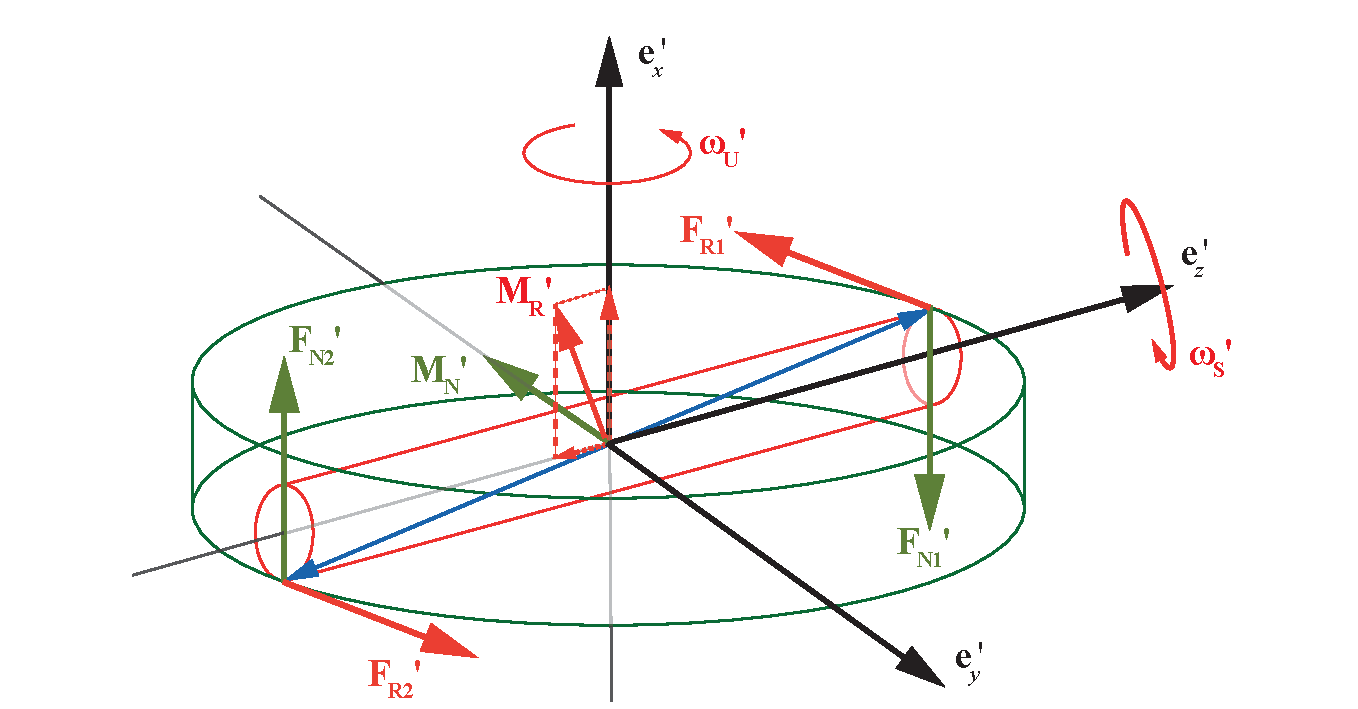
\includegraphics[width=\textwidth]{GyrotwKraefte.pdf}
  \caption[Kr�fte und Drehmomente am Gyrotwister.]{Kr�fte und Drehmomente am
    Gyrotwister bei festgehaltenem Geh�use. Die beiden Auflagekr�fte am
    Nutrand $\vec{F}_{\mathrm{N}1}'$ und $\vec{F}_{\mathrm{N}2}'$ bewirken ein
    Drehmoment, das eine Rotation in der $\vecpeY$-Richtung verhindert. Die
    Reibungskr�fte $\vec{F}_{\mathrm{R}1}'$ und $\vec{F}_{\mathrm{R}2}'$ ergeben
    zusammen mit den zu $\vecpeX$ parallelen Komponenten der Ortsvektoren der
    Auflagepunkte ein Drehmoment  $\vec{M}_\mathrm{R}'$, dessen
    $\vecpeZ$-Komponente eine �nderung von $\omega_S'$ bewirken kann (siehe
    gestrichelt rote Komponenten parallel zur $\vecpeZ$-Achse). Im hier
    gezeigten Fall des nicht bewegten, festgehaltenen Geh�uses zeigt sich
    nur die abbremsende Wirkung der Reibung -- die $z'$-Komponente von
    $\vec{M}_\mathrm{R}'$ wirkt der Drehung entgegen. Das Drehmoment
    $\vec{M}_\mathrm{N}'$, verursacht von den Auflagekr�ften
    $\vec{F}_{\mathrm{N}1}'$ und $\vec{F}_{\mathrm{N}2}'$, kann keine �nderung von
    $\vec{\omega}_\text{s}'$ bewirken, da es senkrecht auf diesem Vektor steht.}.
  \label{abb:bew_GyrotwKraefte}
\end{figure}

Die Bewegung soll mit \figref{bew_GyrotwKraefte} genauer untersucht werden. Dazu folgen wir \cite{Heyda2002}
und w�hlen ein Koordinatensystem $\tilde{\vec{\Sigma}}'$, das sich mit dem Geh�use mitbewegt.
Die $\vecpeX$-Achse steht senkrecht auf der Ebene, in der die Nut liegt. Sie
ist geeignet, um die Drehbewegung des Kreisels aufgrund des Abrollens am
Nutrand zu beschreiben. Die $\vecpeY$-Achse liegt in der Nutebene senkrecht
zur Figurenachse des symmetrischen Kreisels und die $\vecpeZ$-Achse 
entspricht der Figurenachse.
Damit die Lage der $\vecpeY$- und $\vecpeZ$-Achsen zu jeder Zeit so
definiert sein kann, macht das Koordinatensystem die Drehung um die
Figurenachse nicht mit. Das System $\tilde{\vec{\Sigma}}'$ ist also kein vollst�ndig k�rperfestes System des Kreisels.
F�r die Beschreibung der wirkenden Drehmomente und Bewegungen ist es jedoch
hervorragend geeignet. Im gew�hlten Koordinatensystem hat die Bewegung die folgenden Anteile:
\begin{itemize}
\item Die schnelle Rotation des Kreisels erfolgt um die $\vecpeZ$-Achse.
  Sie lautet mit der schnellen Winkelgeschwindigkeit $\omega_\text{S}'$\footnote{Wir kennzeichnen die Vektoren im KOS $\tilde{\vec{\Sigma}}'$ weiterhin als gestrichene Gr��en, die  Winkelgeschwindigkeitskomponenten der Kreiselrotation zur besseren Unterscheidung aber ohne Strich und mit Gro�buchstaben.}
  \begin{equation*}
    \vec{\omega}_\text{S}' = \begin{pmatrix} 0 \\ 0 \\ \Omega_\text{S} \end{pmatrix} \; .
  \end{equation*}
\item Die Rotation durch den Umlauf entlang der Nut entspricht, wie oben
  bereits angemerkt, einer Drehung mit der Umlaufwinkelgeschwindigkeit
  $\omega_\text{U}'$ um die $\vecpeX$-Achse,
  \begin{equation*}
    \vec{\omega}_\text{U}' = \begin{pmatrix} \Omega_\text{U}\\ 0 \\ 0 \end{pmatrix} \; .
  \end{equation*}
\item Zus�tzlich gibt es noch das aktive Eingreifen des Menschen in das
  System durch die Drehbewegung mit der Hand. Wir modellieren diese durch
  eine Drehung um eine raumfeste Achse, die in der Ebene der Nut liegt und deren Lage sich durch die Drehbewegung
  $\vec{\omega}_\text{U}'$ im teilweise k�rperfesten System $\tilde{\vec{\Sigma}}'$ st�ndig �ndert.
  Wir messen die Drehung um die $\vecpeX$-Achse durch den Winkel (\figref{bew_GyrotwAufbau2}b)
  \begin{equation*}
    \varphi_\text{U} = \int_0^t \Omega_\text{U} \,\D t'
  \end{equation*}
  und erhalten damit f�r die Winkelgeschwindigkeit der von der Hand
  verursachten Rotation im KOS
  $\tilde{\Sigma}$
  \begin{equation}
    \vec{\omega}_\text{H}' = \mathbb{R}_{x'}(\varphi_\text{U})\, \vec{\omega}_H
    = \begin{pmatrix} 1 & 0 & 0 \\ 0 & \cos\varphi_\text{U}
      & \sin\varphi_\text{U} \\ 0 & -\sin\varphi_\text{U} & \cos\varphi_\text{U}
    \end{pmatrix} \begin{pmatrix} 0 \\ 0 \\ \Omega_\text{H} \end{pmatrix}
    = \begin{pmatrix} 0 \\ \Omega_\text{H}\,\sin\varphi_\text{U} \\ \Omega_\text{H} \, \cos\varphi_\text{U}
    \end{pmatrix} \; .
    \label{eq:bew_GyrotwRotHand}
  \end{equation}
\end{itemize}
Die gesamte Winkelgeschwindigkeit $\vec{\omega}_\text{ges}'$ des Kreisels lautet damit im KOS $\tilde{\vec\Sigma}'$
\begin{equation*}
  \vec{\omega}_\text{ges}' = \vec{\omega}_\text{S}' + \vec{\omega}_\text{U}' + \vec{\omega}_\text{H}'   =  \begin{pmatrix} \omega_1' \\ \omega_2' \\ \omega_3' \end{pmatrix}
= \begin{pmatrix} \Omega_\text{U} \\ \Omega_\text{H}\,\sin\varphi_\text{U} \\
    \Omega_\text{S} + \Omega_\text{H} \, \cos\varphi_\text{U} \end{pmatrix}
  \; ,
\end{equation*}
wobei $\omega_1'$, $\omega_2'$ und $\omega_3'$ die Komponenten von
$\vec{\omega}_\text{ges}'$ entlang der Achsen $\vecpeX$, $\vecpeY$ und
$\vecpeZ$ darstellen. Hier stellen wir zwei Beziehungen fest. 
\begin{itemize}
	\item Die Rotation durch den Umlauf in der Nut entspricht immer $\omega_1'$. Man kann diese als Pr�zession des symmetrischen Kreisel begreifen. Wir verwenden also im Folgenden die
Identit�ten 
\begin{align}
	\Omega_\text{U} = \omega_1' ~~~ \text{und}  ~~~ \varphi_\text{U} = \varphi_1' = \int_0^t \omega_1' \D t'\,.   \label{eq:bew_Gyrotw_omega1}
\end{align}
\item Zweitens sehen wir, dass $\omega_2'$, also die Rotation um die
  $\vecpeY$-Achse, eindeutig durch die Bewegung der Hand festgelegt ist:
\begin{equation}
  \omega_2' =  \Omega_\text{H}\,\sin\varphi_\text{U}\, \; .
  \label{eq:bew_Gyrotw_omega2}
\end{equation}
Dies ist auch zu erwarten, da die Nut eine freie Rotation um die $\vecpeY$-Achse verhindert.\\
\end{itemize}
F�r die weitere Rechnung und auch den Bezug zu experimentellen Werten ist es sinnvoll, eine geeignete Drehung
$\vec{\omega}_\text{K}'$ im gew�hlten Koordinatensystem $\tilde{\vec{\Sigma}}'$ zu definieren, mit der sich $\vec{\omega}_\text{S}'$  gegen�ber dem raumfesten
System relativ bewegt. Diese Drehung $\vec{\omega}_\text{K}'$ enth�lt nur die Anteile $\vec{\omega}_\text{U}' = \vec{\omega}_1'$ und
$\vec{\omega}_\text{H}'$, nicht jedoch die schnelle Drehung $\vec{\omega}_\text{S}'$ um die
Figurenachse\footnote{Wie oben erw�hnt, haben wir kein echtes k�rperfestes
  Koordinatensystem verwendet. Damit bleibt der Vektor $\vecpey$ immer in der
  Nutebene liegen und die weitere Rechnung �bersichtlich.},
\begin{equation*}
  \vec{\omega}_\text{K}' = \vec{\omega}_\text{ges}' - \vec{\omega}_\text{S}' =
  \begin{pmatrix} \omega_1' \\ \Omega_\text{H}\,\sin\varphi_1' \\
    \Omega_\text{H}\,\cos\varphi_1' \end{pmatrix} \; .
\end{equation*}

Mit den Tr�gheitsmomenten $J_{12}$ f�r Rotationen senkrecht zur Figurenachse
und $J_3$ f�r Rotationen um die Figurenachse lautet der Drehimpuls im teilweise mitbewegten System $\tilde{\vec{\Sigma}}'$:
\begin{equation*}
  \vec{L}' = \begin{pmatrix} J_{12}\: \omega_1' \\ J_{12}\: \omega_2' \\ J_3\: \omega_3' \end{pmatrix} \,.
\end{equation*}

Die Kreiselgleichungen ergeben sich im raumfesten Koordinatensystem aus dem 
\KOS{} $\tilde{\vec{\Sigma}}'$, das mit $\vec{\omega}_\text{K}'$ rotiert,
zu (\vgl \eqref{eq:bew_Rot_System5})
\begin{equation*}
  \frac{\D}{\D t} \vec{L} = \frac{\D}{\D t} \vec{L}' + \vec{\omega}_\text{K}' \times
  \vec{L}' = \MD' \,.
\end{equation*}
Die Ableitung des Drehimpulses im \KOS{} $\tilde{\vec{\Sigma}}$ l�sst sich in Komponenten aufschreiben zu
\begin{align}
  \frac{\D}{\D t} \vec{L}' + \vec{\omega}_\text{K}' \times \vec{L}'
  &= \begin{pmatrix} J_{12}\: \dot{\omega}_1' \\ J_{12}\:
    \dot{\omega}_2' \\ J_3\: \dot{\omega}_3' \end{pmatrix}
  + \begin{pmatrix} \omega_1' \\ \Omega_\text{H}\,\sin\varphi_1' \\
    \Omega_\text{H} \,\cos\varphi_1'\end{pmatrix} \times \begin{pmatrix} J_{12}\:
    \omega_1' \\ J_{12}\: \omega_2' \\ J_3\: \omega_3' \end{pmatrix} \notag \\
  &= \begin{pmatrix}
    J_{12}\:\dot{\omega}_1' + J_3 \:\Omega_\text{H}\,\omega_3'\,\sin\varphi_1'
    - J_{12}\: \Omega_\text{H}\,\omega_2'\,\cos\varphi_1' \\
    J_{12}\:\dot{\omega}_2' + J_{12} \:\Omega_\text{H}\,\omega_1'\,\cos\varphi_1'
    - J_3\: \omega_1'\,\omega_3' \\
    J_3\:\dot{\omega}_3' + J_{12}\: \left (\omega_1'\, \omega_2' - 
      \Omega_\text{H} \,\omega_1' \,\sin\varphi_1'\,\right )
  \end{pmatrix} = \MD'\; .
  \label{eq:bew_Gyrotw_drehimp}
\end{align}
Wir m�ssen jetzt noch das Drehmoment $\MD'$ berechnen, damit wir die Bewegungsgleichung nach den einzelnen $\omega_i(t)'$ l�sen k�nnen. Man kann das Drehmoment in zwei Beitr�ge aufteilen:
\begin{itemize}
\item Die Auflagekr�fte auf der Nut $\vec{F}_{\text{N},i}'$, die verhindern,
  dass eine Rotation um die $\vecpeY$-Achse stattfinden kann, bewirken ein
  Drehmoment $\vec{M}_\text{N}'$.
  Dieses liegt senkrecht zum Ortsvektor der Auflagepunkte (blau in
  \figref{bew_GyrotwKraefte}) und senkrecht zur $\vecpeX$-Achse\footnote{Die
    Kr�fte vom Nutrand auf die Achse sind parallel zu $\vecpeX$ gerichtet.}.
  Es zeigt im Beispiel aus \figref{bew_GyrotwKraefte} in Richtung der
  negativen $\vecpeY$-Achse.
  \begin{equation}
    \vec{M}_\text{N}' = r\,\vecpeZ \times F \,\vecpeX = M_0\, \vecpeY
    \label{eq:bew_GyrotwNutDrehmoment}
  \end{equation}
  Der Betrag $M_0$ dieses Drehmoments muss uns nicht bekannt sein. Vielmehr
  k�nnen wir es sp�ter aus der Bedingung, dass $\omega_2'$ fest durch $\Omega_\text{H}$ gegeben ist,
  berechnen.

  Wir sehen hier �brigens auch eines der Charakteristika des Gyrotwisters.
  Das von den Auflagekr�ften verursachte Drehmoment
  ist ausschlie�lich parallel zu $\vecpeY$ gerichtet und kann somit wie oben erw�hnt auf keinen
  Fall zu einer Beschleunigung der schnellen Drehbewegung $\vec{\omega}_s'$
  beitragen.\footnote{Selbst wenn man ganz korrekt betrachtet, dass der Vektor
    vom Mittelpunkt des Kreisels zu den Auflagepunkten nicht rein in
    $\vecpeZ$-Richtung zeigt, sondern eine $\vecpeX$ Komponente haben muss,
    tr�gt dies nichts zum Drehmoment bei, da der zur Kraft parallele Anteil des
    Ortsvektors kein Drehmoment verursacht, wie man auch leicht am Kreuzprodukt
    erkennen kann.}

\item Die durch die Bewegung der Hand vermittelte Drehung $\vec{\omega}_\text{H}'$ bewirkt ein weiteres Drehmoment $\vec{M}_\text{H}'$, denn sie �ndert
  offensichtlich nach \eqref{eq:bew_Gyrotw_drehimp} alle Drehimpulskomponenten.
  Diesen Teil extrahieren wir und betrachten die �nderungsrate
  $\D \vec{L}'/\D t$, die dieses Drehmoment aufbringen muss,
  \begin{equation}
    \vec{M}_\text{H}' = \vec{\omega}_\text{H}' \times J_{12}\, \vec{\omega}_\text{U}' = \begin{pmatrix}
      0 \\ \Omega_\text{H} \,\sin\varphi_1'\\ \Omega_\text{H}\,\cos\varphi_1' \end{pmatrix}
    \times \begin{pmatrix} J_{12}\:\omega_1' \\ 0 \\ 0 \end{pmatrix}
    =  \begin{pmatrix} 0 \\ J_{12}\: \Omega_\text{H} \,\omega_1' \,\cos\varphi_1' \\
      - J_{12}\: \Omega_\text{H} \,\omega_1'\,\sin\varphi_1' \end{pmatrix} \;.
    \label{eq:bew_GyrotwDefMH}
  \end{equation}
\end{itemize}

Das gesamte Drehmoment $\MD'$ lautet somit
\begin{equation}
  \MD' = \vec{M}_\text{N}' + \vec{M}_\text{H}'
  =  \begin{pmatrix} 0 \\ M_0 + J_{12}\, \Omega_\text{H} \,\omega_1'\,\cos\varphi_1'
    \\ - J_{12}\,\Omega_\text{H} \,\omega_1'\, \sin\varphi_1' \end{pmatrix} \; .\label{eq:bew_GyrotwTotalMD}
\end{equation}
Dies fasst man mit \eqref{eq:bew_Gyrotw_drehimp} zu den
Bewegungsgleichungen f�r die Komponenten der Winkelgeschwindigkeit $\vec{\omega}_\text{ges}'$ zusammen,
\begin{subequations}
  \begin{align}
    J_{12}\, \dot{\omega}_1' &= - J_3\,\Omega_\text{H} \,\omega_3' \,\sin\varphi_1'+
                               J_{12}\, \Omega_\text{H}\, \omega_2' \,\cos\varphi_1'\; ,\\
    J_{12}\, \dot{\omega}_2' &= J_3\, \omega_1' \,\omega_3' + M_0 \; ,
    \label{eq:bew_GyrotwDGLomega2}\\
    J_3\, \dot{\omega}_3' &= - J_{12}\, \omega_1' \,\omega_2' \; .
  \end{align}
\end{subequations}

Wir interessieren uns vor allem f�r die �nderung von $\vec{\omega}_\text{S}'$. Nun wissen wir au�erdem, dass
$\omega_2'$ nach \eqref{eq:bew_Gyrotw_omega2} abh�ngig von anderen Gr��en, \ua  von der Bewegung der Hand ($\Omega_\text{H}$) ist. Benutzen wir die Beziehung \eqref{eq:bew_Gyrotw_omega2}, die $\omega_2'$ mit $\Omega_\text{H}$ koppelt, erhalten
wir die beiden gekoppelten Bewegungsgleichungen f�r $\dot{\omega}_1'$ und  $\dot{\omega}_3'$:
\begin{subequations}
  \begin{align}
    J_{12}\, \dot{\omega}_1' &= - J_3\,\Omega_\text{H} \,\omega_3'\,\sin\varphi_1' +
                               J_{12}\, \Omega_\text{H}^2\,\cos\varphi_1'\,\sin\varphi_1'\; , \label{eq:bew_GyrotwDGLomega1} \\
    J_3\, \dot{\omega}_3' &= - J_{12}\,\Omega_\text{H}\,\omega_1' \,\sin\varphi_1'\; . \label{eq:bew_GyrotwDGLomega3}
  \end{align}
\end{subequations}
Man sieht aus Gl. \eqref{eq:bew_GyrotwDGLomega3}, dass sich die Geschwindigkeit $\omega_3'$ der schnellen Rotation um die $\vecpeZ$-Achse also tats�chlich �ndern kann.
Allerdings besagt Gleichung \eqref{eq:bew_GyrotwDGLomega3} vorerst nur, dass
eine �nderung von $\omega_3'$ m�glich ist. Wie erreichen wir aber gezielt eine
Beschleunigung, \dh ein Anwachsen von $\omega_3'$? Dazu m�ssen wir
sicherstellen, dass $\dot{\omega}_3'$ durchg�ngig dasselbe Vorzeichen hat wie
$\omega_3'$. Gehen wir davon aus, dass zu einem Zeitpunkt am Anfang der
Bewegung $\omega_3' > 0$ und $\omega_1' > 0$ sind (\figref{bew_GyrotwKraefte}),
dann ist die Bedingung f�r eine Beschleunigung ganz sicher erf�llt, wenn
\begin{equation}
  \Omega_\text{H}(t) = - \hat{\Omega}_\text{H}\, \sin \varphi_1'(t)
  \label{eq:bew_Gyrotw_omegaH}
\end{equation}
gilt, worin $\hat{\Omega}_\text{H}$ die Amplitude der Handbewegung und positiv
ist. Dann werden die Bewegungsgleichungen \eqref{eq:bew_GyrotwDGLomega1} und
\eqref{eq:bew_GyrotwDGLomega3} zu
\begin{align}
  J_{12}\, \dot{\omega}_1' &= J_3\,\hat{\Omega}_\text{H} \,\omega_3'\,\sin^2\varphi_1'\,  +\,
                             J_{12}\,\hat{\Omega}_\text{H}^2\,\cos\varphi_1'\,\sin^3\varphi_1'\; , \\
  J_3\, \dot{\omega}_3' &= J_{12}\,\hat{\Omega}_\text{H}\,\omega_1' \sin^2\varphi_1'\;. \label{eq:bew_GyrotwDGLoptomega3}
\end{align}
Das Geheimnis des Gyrotwisters besteht also darin, die Hand immer mit der Frequenz der Rotation
$\omega_1'(t)$ zu bewegen.\footnote{Man  erkennt an \eqref{eq:bew_GyrotwDGLoptomega3} auch sofort, dass bei nicht bewegter Hand ($\hat{\Omega}_\text{H}=0$ sofort $\omega_1 = \mathrm{const}$ (Pr�zession) und $\omega_3 = \mathrm{const}$ (schnelle Kreiselrotation) folgt. Die abbremsenden Reibungskr�fte sind hier nicht modelliert.} Dabei ist die Phasenlage wichtig. Der Winkel $\varphi_1' =
\varphi_\text{U}'$ beschreibt den Umlauf des Kreisels in der Nut. Die Komponente
von $\vec{\omega}_\text{H}'$ entlang der Figurenachse $\vecpeZ$ lautet nach
\eqref{eq:bew_GyrotwRotHand} gerade $\Omega_\text{H}\cos\varphi_\text{U}$.
Die Geschwindigkeit von $\Omega_\text{H}$ ist nach \eqref{eq:bew_Gyrotw_omegaH}
proportional zu $-\sin \varphi_U$. Sie muss der Figurenachse also um
$\pi/2$ vorauseilen.

\begin{figure}
  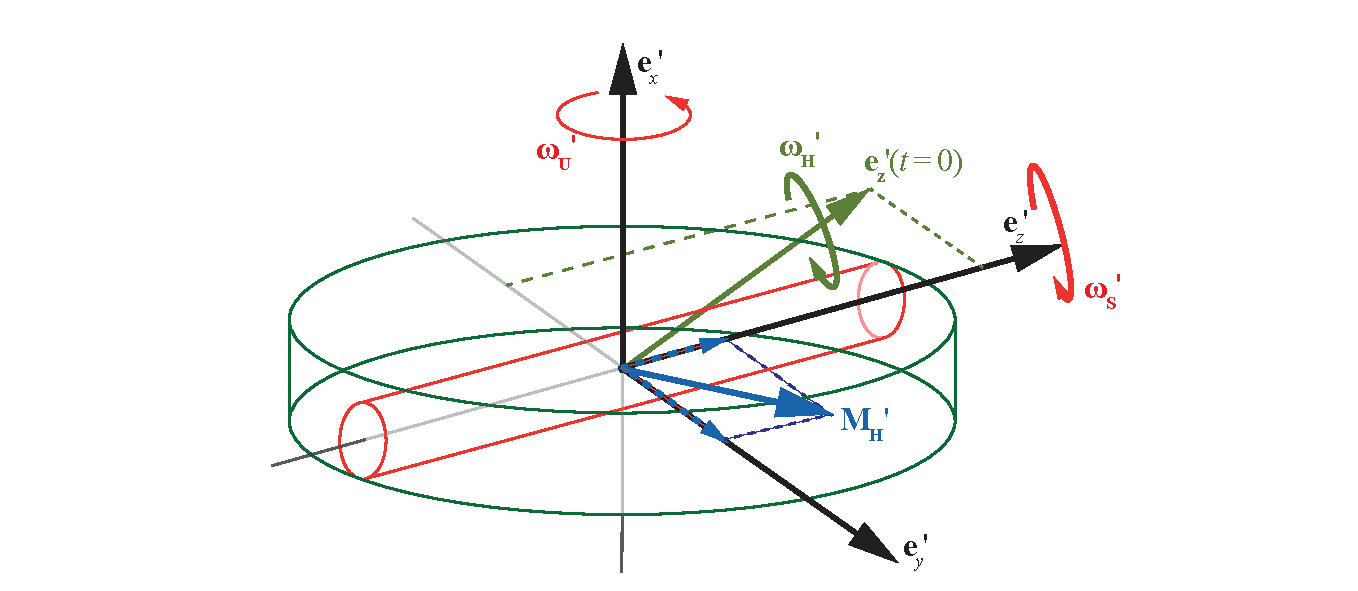
\includegraphics[width=\textwidth]{GyrotwHand.pdf}
  \caption[Bewegung der Hand am Gyrotwister.]{Bewegung der Hand am
    Gyrotwister. Durch die Drehung des Geh�uses entgegen der Drehrichtung
    des Kreisels bewirkt man das Drehmoment $\vec{M}_\text{H}$, das die
    Rotation um die $\vecpeZ$-Achse beschleunigt.}
  \label{abb:bew_GyrotwHand}
\end{figure}

Um physikalisch zu verstehen, warum das gerade zu einer Beschleunigung
f�hrt, betrachten wir noch einmal die wirkenden Kr�fte und Drehmomente.
\figref{bew_GyrotwKraefte} zeigt die Ortsvektoren vom Mittelpunkt
des Kreisels zu einem der Auflagepunkte (blau) sowie die Auflagekr�fte (gr�n)
und die Reibungskr�fte (rot) mit den jeweils sich dazu ergebenden Drehmomenten.
Man erkennt, dass die zu $\vecpeX$ parallele Komponente des Ortsvektors zum
Auflagepunkt zusammen mit den Reibungskr�ften $\vec{F}_{\text{R}1}'$ und
$\vec{F}_{\text{R}2}'$ einen Beitrag zum Drehmoment parallel zu $\veceZ$
leisten kann. Wir erkennen jetzt auch, warum wir ein Lager mit Spiel brauchen.
Die Achse des Kreisels muss sich in der Nut leicht verdrehen k�nnen, sodass
sie nur an einer Seite anst��t. Nur so kann die Abrollbewegung $\omega_1'$
in Gang kommen, die essentiell ist, und eine Beschleunigung der schnellen
Drehung des Kreisels $\omega_3'$ zu bewirken, vgl.
\eqref{eq:bew_GyrotwDGLomega3}. Die oben beschriebene Bewegung des Geh�uses
sorgt nun �ber zus�tzliche Kr�fte durch die Hand daf�r, dass der Kreisel
von der Bewegung des Geh�uses mitgenommen wird und sich das Abrollen
beschleunigt. Dazu schauen wir uns \figref{bew_GyrotwHand} an. Die
Rotationsbewegung der Hand erfolgt nach \eqref{eq:bew_GyrotwRotHand} um
die $\vecpeZ(t=0)$-Achse (gr�ne Achse in der Abbildung), das Drehmoment
ergibt sich dann nach \eqref{eq:bew_GyrotwDefMH} um $\pi/2$ phasenversetzt
(blau). Die Komponente entlang der momentanen $\vecpeZ$-Achse sorgt
f�r die Beschleunigung der Rotation des Kreisels.

Nun wollen wir noch ermitteln, wie gro� der Betrag des von der Nut ausge�bten Drehmoments $\left|\vec{M}_\text{N}'\right| =  M_0$ ist.
Dieser ergibt sich aus der Bedingung, dass Gleichung \eqref{eq:bew_GyrotwDGLomega2}
f�r das $\omega_2'$ aus der Zwangsbedingung \eqref{eq:bew_Gyrotw_omega2}
erf�llt sein muss. Weiterhin wollen wir den Fall \eqref{eq:bew_Gyrotw_omegaH}
betrachten, in dem die maximale Energie eingekoppelt wird. Fasst man alles
zusammen, erh�lt man
\begin{align}
  M_0 &= J_{12}\: \dot{\omega}_2' - J_3\, \omega_1'\, \omega_3' ~~\text{\bzw} \nonumber \\
  M_0 &= -2 J_{12}\: \hat{\Omega}_\text{H}\,\omega_1'\, \cos\varphi_1' \, \sin\varphi_1' \, 
	       - J_3\: \omega_1'\,\omega_3' \;.    \label{eq:bew_gyrotwo_M0}
\end{align}
Es soll betont werden, dass wir in der gesamten Betrachtung die beiden
Winkelgeschwindigkeiten $\omega_1'$  und $\omega_3'$ als unabh�ngig betrachtet
haben. Das widerspricht der Anmerkung vom Anfang, dass die Drehung
$\omega_1'$ durch das Abrollen am Nutrand zustande kommt. Daf�r muss die
Rollbedingung
\begin{equation*}
  \omega_1 = \frac{R_\text{N}}{R_\text{A}}\omega_3
\end{equation*}
durchg�ngig erf�llt sein, wobei $R_\text{N}/R_\text{A}$ das Verh�ltnis des Nutradius zum Achsenradius des Kreisels beschreibt. Die Rollbedingung l�sst 
damit nur eine unabh�ngige Variable zu. Tats�chlich ist das Rollen aber auch nicht
immer erf�llt. Bei h�heren Geschwindigkeiten f�ngt die Achse meist an, am
Nutrand entlang zu rutschen, sodass tats�chlich wieder zwei unabh�ngige
Variablen vorliegen. Liegt ein reines Abrollen vor, muss die zus�tzliche
Zwangsbedingung selbstverst�ndlich ber�cksichtigt werden. Weiterhin haben
wir vernachl�ssigt, dass durch die leichte Schr�glage in der Nut der
Basisvektor $\vecpeX$ streng genommen nicht senkrecht auf der Nutebene steht
und die  Vektoren $\vecpeY$ und $\vecpeZ$ nicht exakt in der Nutebene liegen.
Das hat zur Folge, dass $\vec{\omega}_\text{H}'$ eine (wenn auch sehr kleine)
Komponente in $\vecpeX$-Richtung besitzt. Das ver�ndert die Ergebnisse
jedoch nur geringf�gig \cite{Heyda2002}. Eine Analyse, die dies ber�cksichtigt,
findet sich in \cite{Gulick2000}.

In der numerischen L�sung, die mit dem 
\mscr{} \mlbewref{Gyrotwister.m} erzeugt wurde, sehen wir, dass sich $\omega_3'$ tats�chlich
mit einer positiven Steigung �ndert.
Dies ist in Abbildung \figref{bew_Gyrotwomega3} dargestellt.

\begin{figure}
  \centering
  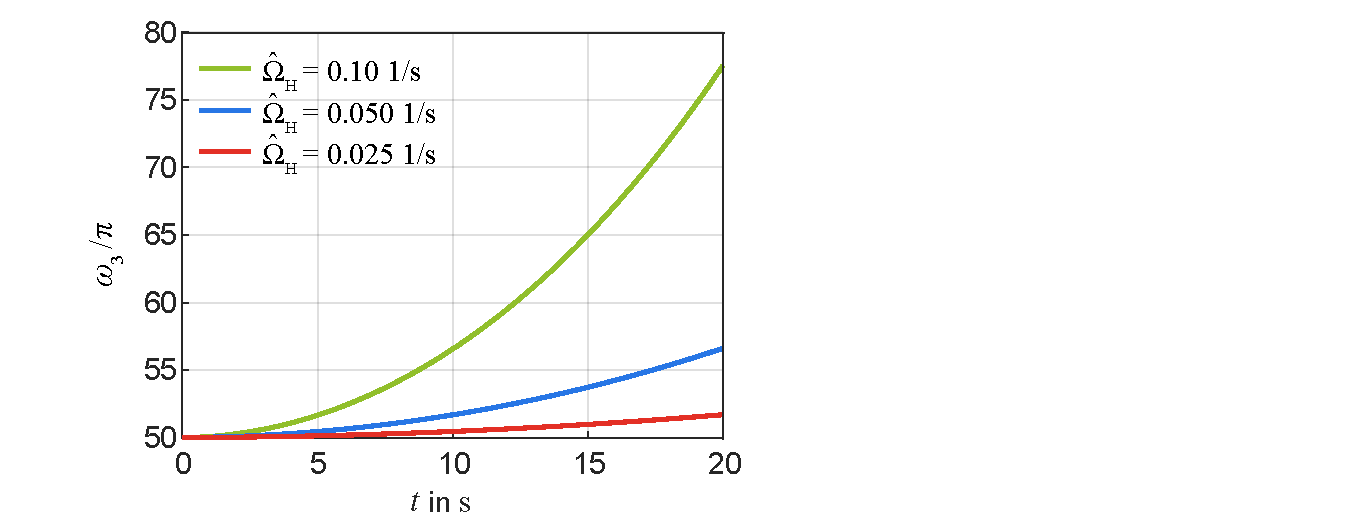
\includegraphics[width=\textwidth]{Gyrotwister1.pdf}
  \caption[Beschleunigung des Kreisels im Gyrotwister.]{Beschleunigung des
    Kreisels im Gyrotwister durch die Bewegung mit der Hand. Hier wird die
    optimale Einkopplung an Energie nach Gleichung \eqref{eq:bew_Gyrotw_omegaH}
    angenommen. Die Frequenz $\omega_3'$ steigt offensichtlich mit der Zeit an. Parameter siehe \mscr{} \mlbewref{Gyrotwister.m} }
  \label{abb:bew_Gyrotwomega3}
\end{figure}

Man kann auch gut erkennen, dass eine Phasendifferenz entscheidend f�r die
Beschleunigung ist.
Die Berechnungen dazu sind im \mscr{} \mlbewref{GyrotwisterPhase.m} zu finden.
In Abbildung \figref{bew_GyrotwPD} (links) ist der damit ermittelte Zeitverlauf von
$\omega_3'$ f�r verschiedene Phasendifferenzen $\Delta\phi$ zum optimalen Fall
\begin{equation}
  \Omega_\text{H} = - \hat{\Omega}_\text{H}\, \sin \left ( \varphi_1' +\Delta \phi \right )
  \label{eq:bew_Gyrotw_omegaHdiff}
\end{equation}
aufgetragen.
F�r $\Delta\phi = 0.2\pi$ ist der Anstieg von $\omega_3'$ erkennbar reduziert.
Bewegt man die Hand um $\Delta\phi=\pi/2$ phasenverschoben
zum optimalen Fall (also um $\pi/2$ Phasenverschoben zur Bewegung von
$\omega_1'$), so koppelt man im Mittel keine Energie ein.
Die Frequenz $\omega_3'$ �ndert sich gar nicht.
Das tut sie jedoch wieder f�r eine
Phasenverschiebung von $\Delta\phi=\pi$.
Auf den ersten Blick mag das �berraschen.
Intuitiv w�rde man einen negativen Effekt erwarten.
Schaut man sich die Bewegung von $\omega_1'$ an, erkennt man auch, dass genau das der
Fall ist (Abbildung \figref{bew_GyrotwPD} rechts).
Die Rotation $\omega_1'$
kehrt sich in diesem Fall um und wird in die entgegengesetzt Richtung beschleunigt.
Dann ist man zwar immer noch mit $\omega_1'$ synchron, aber
es tritt jetzt die ben�tigte Phasenverschiebung zu $\omega_3'$ auf, um wieder
eine Beschleunigung erzielen zu k�nnen.
In Gleichung
\eqref{eq:bew_GyrotwDGLoptomega3} heben sich das Minuszeichen durch die
Phasenverschiebung um $\pi$ aus Gleichung \eqref{eq:bew_Gyrotw_omegaHdiff}
und das Minuszeichen von $\omega_1'$ gegenseitig auf.

\begin{figure}
  \centering
  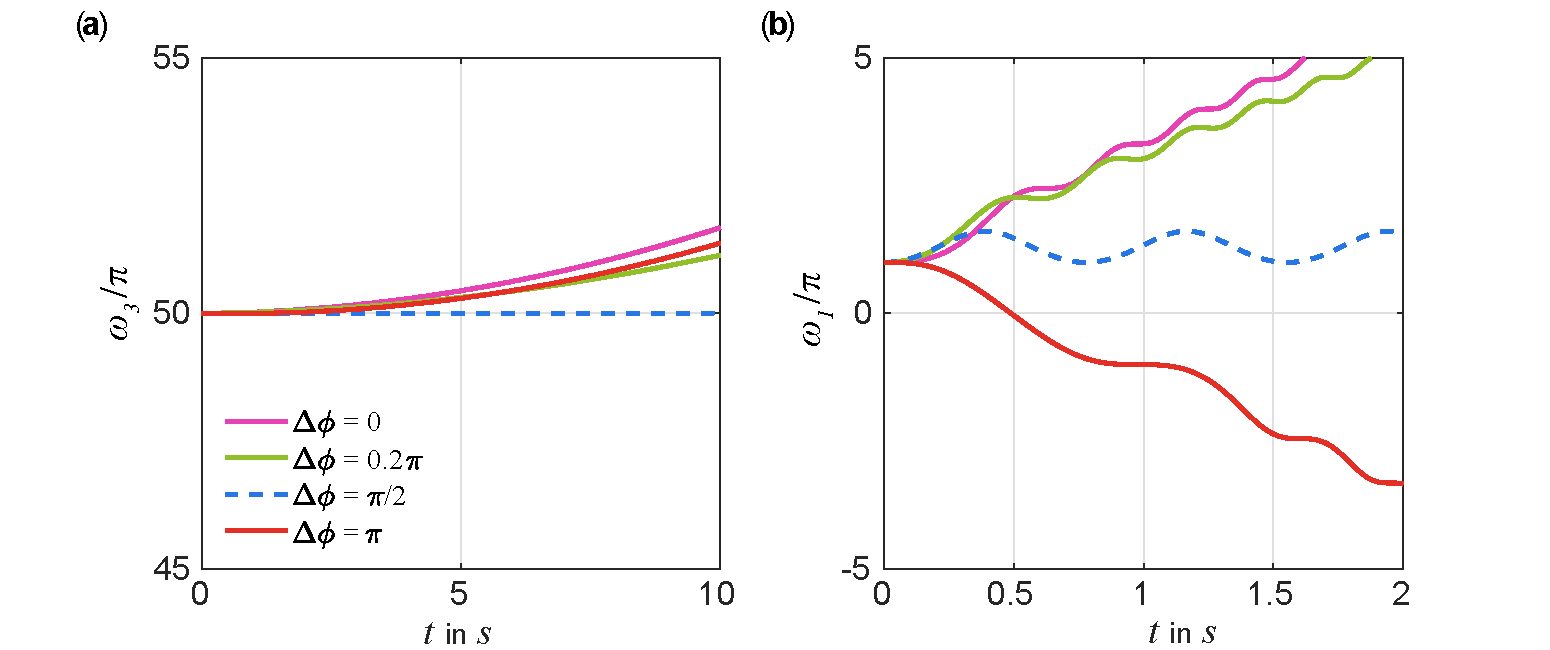
\includegraphics[width=\textwidth]{Gyrotwister2.pdf}
  \caption[Beschleunigung des Kreisels im Gyrotwister mit Phasendifferenz.]
  {\fa Beschleunigung des Kreisels im Gyrotwister mit einer Phasendifferenz
    $\Delta\phi$ zum optimalen Fall nach \eqref{eq:bew_Gyrotw_omegaHdiff}
    und zugeh�rige \fb Entwicklung von $\omega_1'$ (rechts). Nur f�r
    den optimalen Fall $\Delta\phi=0$ erzielt man die maximale Beschleunigung
    von $\omega_3'$. F�r andere Phasenbeziehungen ist sie abgeschw�cht, im
    Fall $\Delta\phi=\pi/2$ verschwindet sie sogar vollst�ndig. F�r
    $\Delta\phi=\pi$ sorgt die Umkehrung der Rotationsrichtung von
    $\omega_1'$ daf�r, dass wieder eine Beschleunigung eintritt.}
  \label{abb:bew_GyrotwPD}
\end{figure}

M�chte man nur grobe qualitative Ergebnisse erhalten, kann man davon
ausgehen, dass $\Omega_\text{H}(t)$ sich im Vergleich mit der schnellen Rotation
des Kreisels nur langsam ver�ndert \cite{Heyda2002}, was eine vern�nftige
Annahme ist. Dann kann man auch mittlere
Frequenzen $\bar{\omega}_1'$ und $\bar{\omega}_3'$ einf�hren und es gilt $\varphi_1' = \bar{\omega}_1'
\,t$. Die Absch�tzungen f�r die Beschleunigung der
Kreiselrotation lauten damit:
\begin{align*}
  \frac{\Delta \bar{\omega}_3'}{\Delta t} &= \lk \frac{1}{2\pi} \int_0^{2\pi} \sin^2\varphi_1'\,\D\varphi_1' \rk \, \frac{J_{12}}{J_3 } \, \hat{\Omega}_\text{H} \, \bar{\omega}_1' 
                                           = \frac{1}{2} \frac{J_{12}}{J_3 } \,\hat{\Omega}_\text{H} \,\bar{\omega}_1'\\
  \intertext{bzw. f�r das Drehmoment $\bar{M}_0 $}
  \bar{M}_0 &= - J_3 \:\bar{\omega}_1'\, \bar{\omega}_3' \; .
\end{align*}

In \probref{bew_gyrotwister} wollen wir den Gyrotwister als Trainingsger�t betrachten und die Kr�fte und die Muskelarbeit berechnen, die man bei einem Gyrotwister aufbringen muss, und dies zu einem vergleichbaren Training mit Heben einer Hantel mit einer Masse von $\SI{3}{\kg}$ in Beziehung setzen.


\newpage
\subsection{Der Kreiselkompass, ein nordsuchender Kreisel} \index{Kreisel!nordsuchender}\index{Kreiselkompass} \label{kap:bew_gyro}

\textbf{Zur Geschichte des Kreiselkompasses}\\

Unter einem klassischen Gyroskop\index{Gyroskop} (Kreiselinstrument) versteht man einen schnell rotierenden, symmetrischen Kreisel, der sich in einem beweglichen Lager, \zb einer kardanische Aufh�ngung\index{Aufh�ngung!kardanische} befindet. 
Das erste Gyroskop wurde 1810 von J.G.F.~Bohnenberger\footnote{Johann Gottlieb Friedrich Bohnenberger (1765--1831) war ein deutscher Astronom, Mathematiker, Mechaniker und Physiker, der auch als Geod�t wichtige Beitr�ge erbrachte. Er gilt als Begr�nder der Landesvermessung W�rttembergs.}\indexp{Bohnenberger, Johann Gottlieb Friedrich} an der Universit�t T�bingen erfunden \cite{Wagner2005} und 1852 von L.~Foucault\indexp{Foucault, Jean Bernard L�on} weiterentwickelt (\figref{bew_GyroBohnenberger}b). Diese Ger�te bilden den Ursprung aller sp�teren Kreiselger�te
%f�r die beiden Anwendungsgebiete Navigation und Stabilisierung. Dies betrifft die 
wie Kreiselkompasse, k�nstliche Horizonte und Wendezeiger f�r die Navigation oder auch Kreiselstabilisatoren f�r die Schiff- und Raumfahrt. Selbst die heute in vielen Smartphones und Drohnen eingebauten Inertialplattformen gehen letztendlich auf das Gyroskop-Prinzip zur�ck \cite{Wagner2023}.\\
Interessanterweise war das Gyroskop zun�chst ein Ger�t der physikalischen Grundlagenforschung und Lehre. Es dauerte fast 100 Jahre bis zum Anfang des 20. Jahrhunderts, bis die ersten technischen Anwendungen in der Navigation m�glich wurden (\probref{bew_gyroskope}). 

\begin{figure}
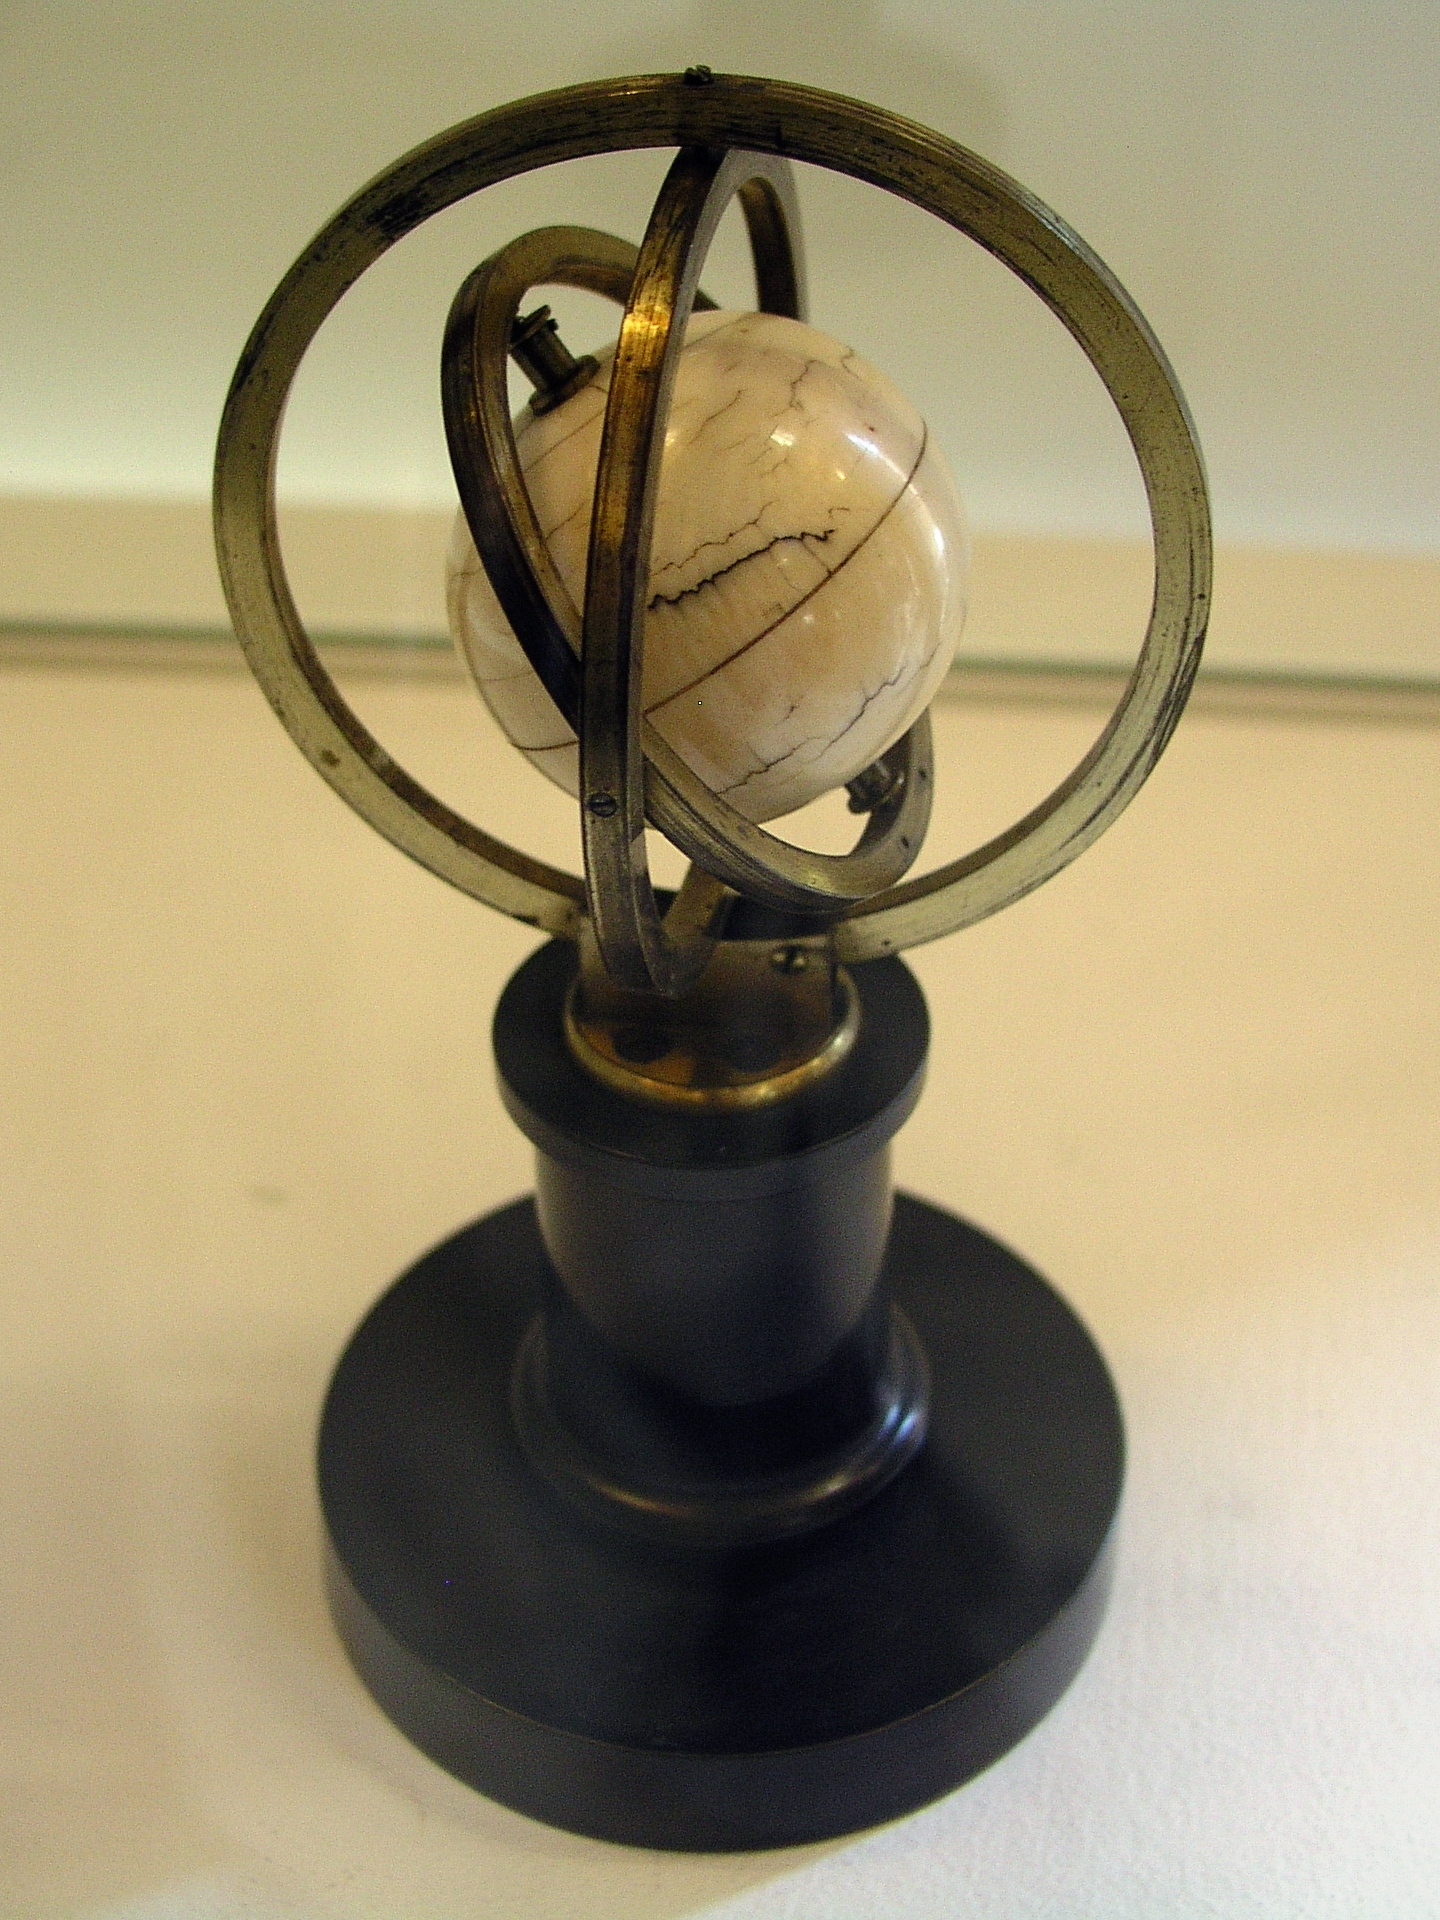
\includegraphics[width=\textwidth]{GyroBohnenberger.pdf}
\caption[Original-Gyroskop von Bohnenberger und Kugelkreiselkompass.]{\fa Das Original-Gyroskop von J.G.F.~Bohnenberger. Ein Exemplar steht im T�binger Stadtmuseum. \fb Foucault's Variante des Gyroskops von Bohnenberger. Freundliche �berlassung von J.F Wagner \cite{Wagner2005, Wagner2023}. \fc Kugelkreiselkompass der Firma Ansch�tz.} %\bzw Wikimedia Commons.
\label{abb:bew_GyroBohnenberger}
\end{figure}

Die Nutzung eines Kreisels f�r die Navigation in der Schifffahrt
hatte zu Beginn des 20.~Jahrhunderts enorme
Bedeutung gewonnen, insbesondere weil ein magnetischer Kompass in der N�he der
Pole zu ungenau ist und in U-Booten mit ihrer Metallh�lle �berhaupt nicht funktioniert.
Hermann Ansch�tz-Kaempfe\indexp{Ansch�tz-Kaempfe, Hermann}%
\footnote{Hermann Ansch�tz-Kaempfe (1872--1931) war ein deutscher Wissenschaftler, der 1905 in Kiel das Unternehmen Ansch�tz \& Co gr�ndete, welches er bis 1930 leitete und dann an die Carl-Zeiss-Stiftung �bertrug. 
%Heute geh�rt das Unternehmen zur Raytheon Gruppe. 
Ansch�tz-Kaempfe entwickelte zusammen mit seinem Vetter Max Schuler den ersten bordtauglichen Kreiselkompass, der 1907 vorgestellt wurde. Ab 1919 wurde daraus der nach Ansch�tz-Kaempfe benannte \anf{Ansch�tz-Zweikreisel-Kugelkompass}.
Dieser Kompass diente als Grundlage moderner Kreiselkompass-Systeme.}
baute als erster auf Basis eines Kreisels einen verl�sslichen Kompass\cite{Lohmeier1992}, der sich selbstt�tig nach Norden ausrichtet.\footnote{Ein Patent f�r die Entwicklung von Ansch�tz-Kaempfe wurde 1904
  angenommen. In einem Patentstreit mit einem amerikanischen Erfinder eines 
  Konkurrenzproduktes wurde Albert Einstein\indexp{Einstein, Albert} als Gutachter hinzugezogen. Aus den Gespr�chen ist
  ein enger Kontakt zwischen Hermann Ansch�tz-Kaempfe und Albert Einstein entstanden, der zu
  zahlreichen Diskussionen �ber die technische Verbesserung des Kreiselkompasses f�hrte
  \cite{Lohmeier1992}.}\\ 
Diese elektromechanischen Kreiselkompasse waren zu ihrer Zeit und sind es auch heute noch wahre Wunderwerke der Mechanik. Ihre Kreiselachsen sind h�ufig f�r die notwendige horizontale Fixierung in komplexen Konstruktionen oder Fl�ssigkeiten gelagert und werden mit elektrischen Motoren mit Drehzahlen bis zu $\SI{75000}{\per\minute}$ angetrieben. Die Orientierungsgenauigkeit ist besser als 10 Winkelsekunden pro Tag, wobei die Einstellzeit des Kreisels auf Nord durchaus einige Stunden betragen kann. \cite{BergmannSchaefer1998}\\

\textbf{Physikalisches Prinzip des klassischen Kreiselkompasses}\\

Um zu verstehen, warum sich ein solcher Kreisel �berhaupt nach Norden
ausrichtet, muss man ber�cksichtigen, dass sich der Kreisel in einem
Nichtinertialsystem befindet. Bisher hatten wir alle Kreisel
nur in einem Inertialsystem betrachtet.
Wir wollen zun�chst eine qualitative physikalische Beschreibung der
Funktionsweise eines Kreiselkompass auf Basis der Newtonschen Mechanik geben
und anschlie�end eine quantitative Rechnung im Lagrange-Formalismus zeigen.\\

Wir betrachten zun�chst das Verhalten eines sogenannten frei drehbaren Kreisels\index{Kreisel!freier}\index{Gyroskop!freies} nach \figref{bew_GyroBohnenberger}a und \figref{bew_GyroCompassExpl01}a. Dessen Drehimpuls bleibt relativ zum Inertialsystem unver�ndert im Raum orientiert, da auf ihn wegen der entsprechenden Lagerung kein Drehmoment wirkt. Wenn er auf einen Stern ausgerichtet war, dann bleibt er auch unabh�ngig von seiner Mitbewegung auf der Erdoberfl�che auf diesen Stern ausgerichtet. F�r einen mitbewegten Erdbeobachter erscheint es daher so, als w�rde ein Ende der Kreiselachse im Laufe eines Tages im Osten aufgehen und im Westen untergehen.\\
\begin{figure}
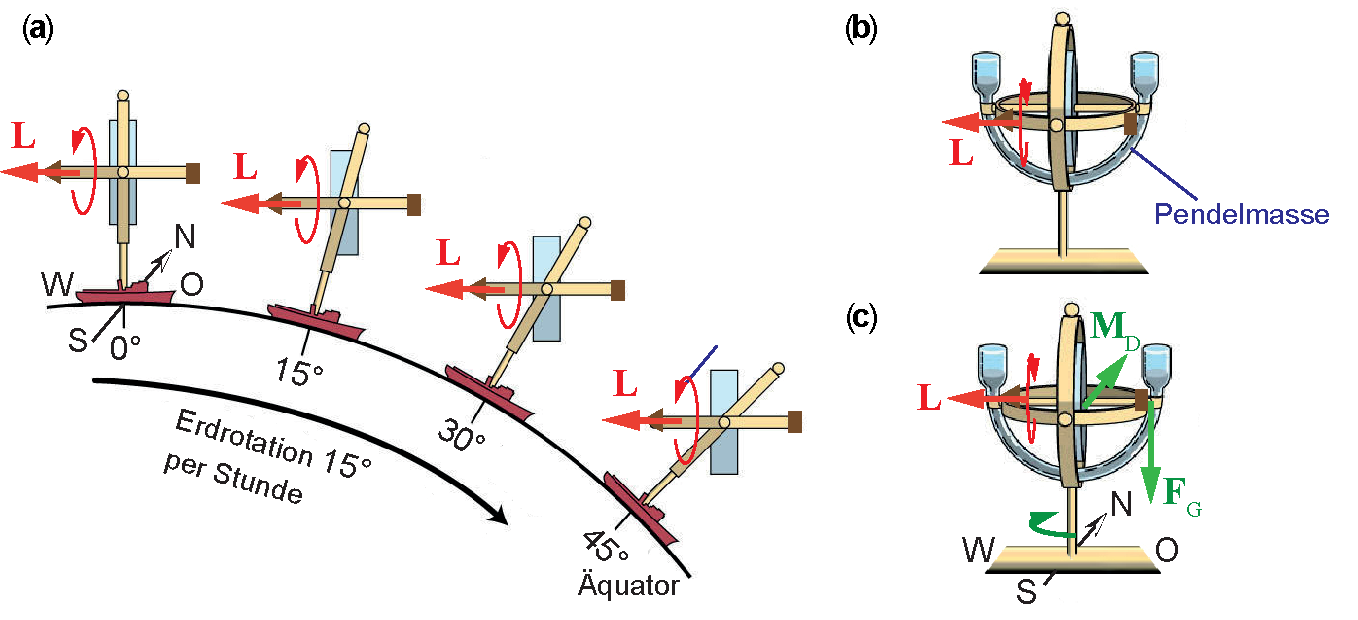
\includegraphics[width=\textwidth]{GyroCompassExpl01.pdf}
\caption[Vergleich freier und Pendelkreisel.]{Vergleich freier und Pendelkreisel. \fa Freier Kreisel auf �quator. \fb Pendelkreisel als Beispiel f�r einen eingeschr�nkten schweren Kreisel. \fc Eine Kraft $\vec{F}_\text{G}$ bewirkt bei einem eingeschr�nkten schweren Kreisel ein Drehmoment $\vec{M}_\text{D}$ in N-Richtung und eine entsprechende Pr�zession. Nach \cite{SFMaritimeNP1946, Britannica2019}.}
\label{abb:bew_GyroCompassExpl01}
\end{figure}

Worin unterscheidet sich nun ein Kreiselkompass von einem frei drehbaren Kreisel? 
Beim Kreiselkompass wird die Bewegung des Kreisels durch die Schwerkraft und eine Zwangsbedingung auf die Horizontebene eingeschr�nkt, \dh die Figurenachse bleibt immer in der Horizontebene liegen, kann sich dort aber frei drehen.
Eine solche Zwangsbedingung kann \zb durch eine entsprechend konstruierte Aufh�ngung (\figref{bew_GyroCompassExpl01}b) realisiert werden.\footnote{Die Designs vieler Kreiselkompasse unterscheiden sich gerade auch in der Realisierung der horizontalen Fixierung.} In diesem Fall haben wir ein sogenanntes Kreiselpendel \index{Kreiselpendel} als Beispiel f�r einen \emph{eingeschr�nkten schweren Kreisel}\index{Kreisel!eingeschr�nkter schwerer}.\\
Wir nehmen nun an, dass dieser Kreisel fest am �quator verankert und seine Rotationsachse in Ost-West-Richtung (O-W) ausgerichtet ist. 
Der Drehimpulsvektor des Kreisels $\vec{L}$ zeigte nach W, was dann der Fall ist, wenn die Eigenrotation des Kreisels bei Blickrichtung von O nach W im Uhrzeigersinn erfolgt (siehe \figref{bew_GyroCompassExpl01}c). 
Die Rotation der Erde von W nach O f�hrt dann dazu, dass aus Sicht eines auf dem Kreisel mitbewegten und in die inititale Westrichtung schauenden Beobachters die Westseite der Horizontebene relativ zur anf�nglich auch im Erdsystem bewegungslosen Kreiselrotationsachse ansteigt, w�hrend die Ostseite absinkt. 
Diese �nderung der Horizontebene bewirkt ein Drehmoment $\vec{M}_\text{D}$ auf den Kreisel.  Man kann sich an Hand von \figref{bew_GyroCompassExpl01}c leicht klar machen, dass dieses Drehmoment parallel zur Erdachse ausgerichtet ist und nach Norden zeigt. Das Drehmoment bewirkt eine Pr�zession des Drehimpulsvektors des Kreisels $\vec{L}$ in Richtung Norden, der Kreisel dreht sich in der Horizontebene im Uhrzeigersinn. Da dieses Drehmoment vom ersten Moment an wirkt und wir annehmen, dass die Pr�zession sofort einsetzt, kommt es in Wirklichkeit nicht zu einer solchen Schr�glage des Kompasses wie in den Stellungen II und III von \figref{bew_GyroCompassExpl02}a gezeigt, sondern der Kreisel ist gezwungernerma�en immer in der Horizontebene ausgerichtet, dreht sich aber in Richtung Norden.\footnote{Wir gehen davon aus, dass bei einer noch so kleinen "`Verkippung"' die "`korrigierende"' Pr�zession instantan erfolgt.}

\begin{figure}
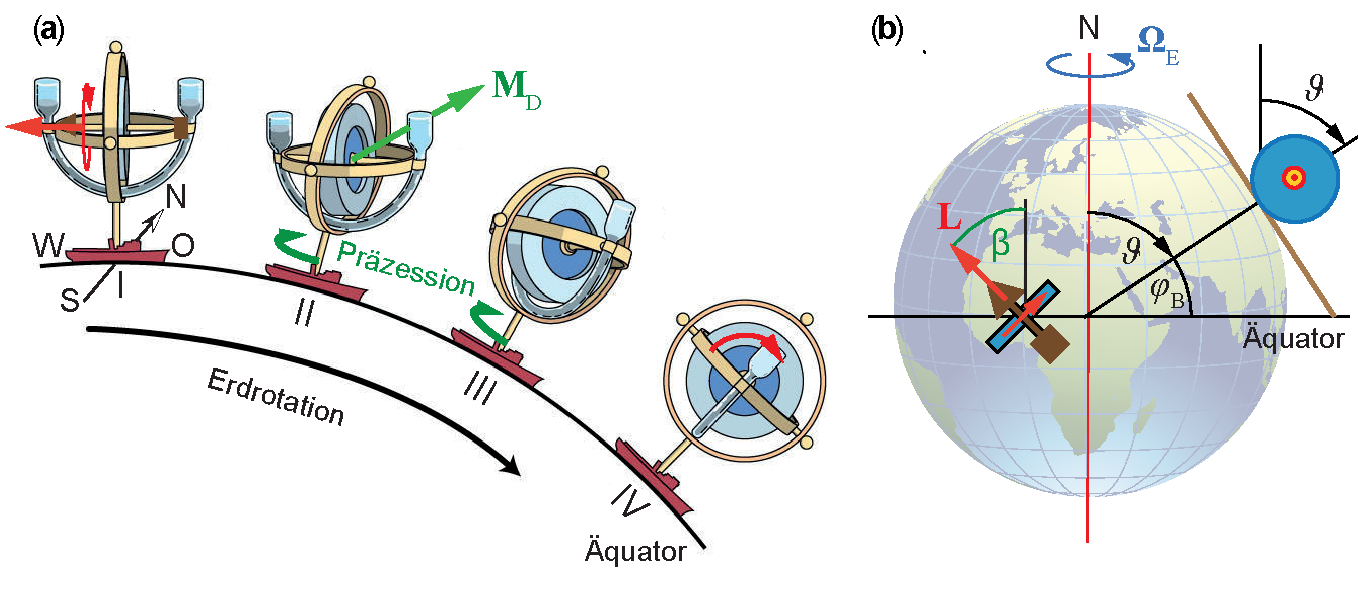
\includegraphics[width=\textwidth]{GyroCompassExpl02.pdf}
\caption[Zum Prinzip des Kreiselkompass.]{Zum Prinzip des Kreiselkompass. \fa Eingeschr�nkter schwerer Kreisel auf der �quator. Ausgangssituation (I), tempor�re virtuelle "`Verkippungen"' (II,III) mit resultierendem Drehmoment und Pr�zessionsrichtung und stabiler Endzustand mit Nordausrichtung (IV). \fb Kreisel auf �quator und Breitengrad. Nach \cite{SFMaritimeNP1946, Rueckner2017,Britannica2019}.}
\label{abb:bew_GyroCompassExpl02}
\end{figure}
Dies passiert bei kontinuierlicher Rotation der Erde solange bis der Kreisel auf Nord-S�d-Richtung ausgerichtet ist (\figref{bew_GyroCompassExpl02}a (IV)). Es kann passieren, dass der Kreisel �ber diesen Punkt ($\vec{M}_\text{D}=0$) hinausl�uft. Dann entsteht ein Gegenmoment $\vec{M}_\text{D} < 0$ und der Kreisel versucht sich wieder nach N  auszurichten. Letztlich wird sich die Kreiselachse bei entsprechender D�mpfung auf die Nord-S�d-Richtung einstellen. Ein solch beschriebener Kreisel wird also durch die Rotation der Erde um ihre Achse so beeinflusst, dass er sich immer nach Norden ausrichtet (daher auch der Name \emph{nordsuchender Kreisel})\footnote{Wir werden gleich sehen, dass der Kreisel sich bei bestimmten Verh�ltnissen mit seinem Eigendrehimpulsvektor auch auf S�den ausrichten kann, in jedem Fall richtet er sich auf die Nord-S�d-Linie (Meridian) aus.} und im Gegensatz zum magnetischen Kompass exakt zum geographischen und nicht zum magnetischen Nordpol ausgerichtet ist.\\
Befindet sich der Kreisel nicht am �quator, sondern auf einem Breitengrad $\varphi_\text{B} = 90\degree - \vartheta$, dann ist die Horizontebene um 
den Winkel $\varphi_\text{B}$ gegen�ber der Erdrotationsachse geneigt (\figref{bew_GyroCompassExpl02}b) und das Drehmoment $\vec{M}_\text{D}$ ist um den Faktor $\cos\varphi_\text{B} = \sin\vartheta$ verkleinert und wird mithin am Nordpol Null. Kreiselkompasse k�nnen also am Pol nicht funktionieren.\\

\textbf{Berechnung der Dynamik des nordsuchenden Kreisels}\\

Wir wollen uns nun den schematischen Aufbau eines Kreiselkompasses nach \figref{bew_KreiselkompSchematisch}a anschauen. Im Gegensatz zum oben skizzierten Pendelkreisel (\figref{bew_GyroCompassExpl01}b) haben wir hier die Situation, dass die konstante Lage der Kreiselachse (Figurenachse) in der Horizontebene durch eine schwimmende Lagerung realisiert wird. Durch diese Lagerung kann sich die Kreiselachse frei in den horizontalen Richtungen $x, y$ drehen.
Der Schwerpunkt des S des Kreisels befindet sich jedoch unter dem
geometrischen Mittelpunkt A der Anordnung, an welcher der Auftrieb angreift. 
Wir haben es deshalb auch hier mit einem (eingeschr�nkten) schweren Kreisel\index{Kreisel!schwerer} zu tun, der sich 
aufgrund der Schwerkraft mit seiner Figurenachse �hnlich dem Pendelkreisel immer in der Horizontebene ausrichten wird (\figref{bew_KreiselkompSchematisch}b).

\begin{figure}
  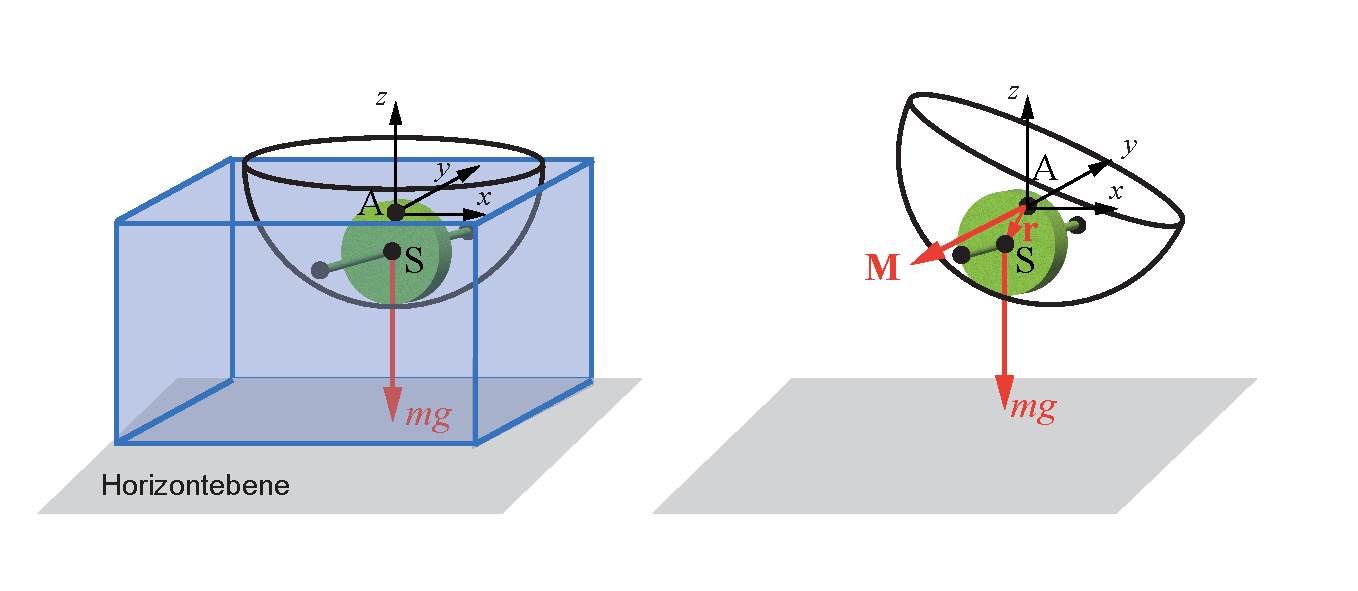
\includegraphics[width=\textwidth]{KreiselkompAufbau.pdf}
  \caption[Schematischer Aufbau des Kreiselkompasses.]{Schematischer Aufbau des
    Kreiselkompasses. Der Kreisel ist hier schwimmend derart gelagert,
    dass die Figurenachse immer in der horizontalen Ebene zu liegen kommt. Dies
    wird durch die Gewichtskraft bewirkt, denn der Schwerpunkt ist unterhalb
    des geometrischen Mittelpunkts des schwimmenden Geh�uses A, an dem der
    Auftrieb angreift, angeordnet. Dies bewirkt sofort ein korrigierendes
    Drehmoment $\vec{M}_\text{D}$, falls eine Auslenkung aus der horizontalen Ebene
    heraus auftreten sollte. In der horizontalen Ebene kann die Figurenachse
    frei rotieren.}
    \label{abb:bew_KreiselkompSchematisch}
\end{figure}

Wie beschrieben entsteht durch �nderung der Richtung der Schwerkraft aufgrund der Rotation der Erde ein Drehmoment, das eine Drehimpuls�nderung zur Folge hat. Die Drehimpuls�nderung erfolgt nur als Rotation um den Punkt A in der horizontalen Ebene. \\

F�r die Berechnung der Dynamik, wie sich ein solcher eingeschr�nkter Kreisel nach Norden
ausrichtet, betrachten wir den Kreisel im Nichtinertialsystem\index{Nichtinertialsystem} der rotierenden Erde. 
Man muss f�r die Aufstellung der Lagrange-Funktion\index{Lagrange-Funktion} alle Rotationen, \dh alle
Drehimpulse, zus�tzlich zum im Inertialsystem betrachteten Eigendrehimpuls, ber�cksichtigen. 
Insbesondere muss der Drehimpuls aufgrund der Rotation der Erde
hinzuaddiert werden.\footnote{Siehe
\zb \cite{Mueller2020} f�r eine ausf�hrliche Betrachtung.}

F�r die entstehende komplizierte Bewegung des Kreisels 
betrachten wir alle m�glichen Drehbewegungen im \textit{k�rperfesten Hauptachsensystem} \index{Hauptachsensystem} und 
setzen dieses in Bezug zu einem raumfesten Koordinatensystem (Inertialsystem).
Die einzelnen, sich �berlagernden, Drehbewegungen werden nun schrittweise
eingef�hrt.\footnote{Es w�rde sich auf den ersten Blick anbieten,
  wieder auf die Eulerwinkel oder zumindest �hnliche Definitionen 
  zur�ckzugreifen, um die Bewegung zu beschreiben.
  Da wir jetzt jedoch explizit ber�cksichtigen m�ssen, dass das mit der
  Erde verbundene Koordinatensystem kein Inertialsystem ist und die Bewegungen
  aufgrund der Einschr�nkung auf eine Ebene komplizierter ausfallen, sind die
  Euler-Winkel hier weniger geeignet. Um eine Verwechslung zu vermeiden, f�hren wir
  neue Bezeichnungen $(\alpha,\,\beta,\,\vartheta)$ ein.} 

\begin{figure}
  \includegraphics[width=\textwidth]{KreiselkompKS.pdf}
  \caption[Koordinatensysteme f�r den Kreiselkompass.]{Koordinatensysteme f�r
    den Kreiselkompass. \fa Ber�cksichtigung der Erddrehung f�r einen
    Kreiselkompass am Nordpol. \fb Auf dem Breitengrad, auf
    dem sich der Kompass nun befindet, soll die $z''$-Achse zum Zenit zeigen. \fc
    Bewegung des Kreiselkompasses in der Horizontebene mit freiem
    Drehwinkel $\beta$. \fd Schnelle Rotation um die Figurenachse $x'''= x''''$,
    ausgedr�ckt durch den Winkel $\alpha$.}
    \label{abb:bew_KreiselkompKS}
\end{figure}

Das k�rperfeste Koordinatensystem des Kreiselkompasses der Halbkugel in \figref{bew_KreiselkompSchematisch} (es wird nachstehend das System $\vec{K}'''$ sein) muss deren Orientierung immer relativ zu dem Ort beschreiben,
an dem sich der Kompass befindet. Dann k�nnen wir aus dieser Beschreibung Navigationsinformationen ablesen. 
Wir beginnen mit dem raumfesten Koordinatensystem $\vec{K}$. 
Im ersten Schritt zum �bergang in das k�rperfeste Koordinatensystem 
ber�cksichtigen wir eine Drehung um die
$z$-Achse, um der Drehung der Erde zu folgen. Es ergibt sich
das Koordinatensystem $\vec{K}'$ (siehe \figref{bew_KreiselkompKS}~a). 
Der Ort des ortsfesten Kreisels liegt auf einem festen Breitengrad, das Koordinatensystem wird so
gew�hlt, dass die $z''$-Achse des Koordinatensystems $\vec{K}''$ 
dort zum Zenit zeigt. Die Transformation erfolgt durch eine
Drehung um die $x'$-Achse (\figref{bew_KreiselkompKS}~b). Der Kompass
kann sich nun um die $z''$-Achse frei bewegen. Dies soll durch den Winkel
$\beta$ ausgedr�ckt werden (\figref{bew_KreiselkompKS}~c). Schlie�lich
muss in einem k�rperfesten System (Koordinatensystem $\vec{K}''''$)
noch ber�cksichtigt werden, dass die schnelle
Rotation des Kreisels um die $x'''$-Achse zu einer Ver�nderung der Achsen
$y'''$ und $z'''$ f�hrt. Die schnelle Rotation wird durch den Winkel $\alpha$
beschrieben (\figref{bew_KreiselkompKS}~d). 

Zun�chst wollen wir uns mit dem Fall besch�ftigen, dass der Kreiselkompass
fest an einem Punkt auf der Erdoberfl�che steht. Das hei�t, dass $\vec{\Omega}_\text{E}$
immer exakt der Rotation der Erde um ihre Achse entspricht (also keine
Bewegung entlang eines Breitengrades erfolgt) und $\vartheta$ ein
unver�nderlicher Winkel ist (also keine Bewegung entlang eines L�ngengrades
erfolgt). Sp�ter werden wir auf bewegte Objekte wie Schiffe und Flugzeuge
eingehen.

Zur Figurenachse $x'''=x''''$ geh�rt das Haupttr�gheitsmoment $J_1$. Die
beiden dazu senkrechten, identischen Tr�gheitsmomente bezeichnen wir mit
$J_{23}$. \\
Dann lauten die einzelnen Drehbewegungen ausgedr�ckt durch die $\vec{\omega}_{\alpha,\beta,\text{E}}$ wie folgt:
\begin{itemize}
\item Die schnelle Rotation des Kreisels um seine Haupttr�gheitsachse $x''''$
  mit dem Winkel $\alpha$ ist zu ber�cksichtigen.
  Die zugeh�rige Winkelgeschwindigkeit
  ist bereits im k�rperfesten System gegeben:
  \begin{equation*}
    \vec{\omega}_\alpha'''' = \begin{pmatrix} \dot{\alpha}\\ 0 \\ 0
    \end{pmatrix} \,.
  \end{equation*}
\item Die freie Bewegung der Figurenachse in der horizontalen Ebene wird
  durch den Winkel $\beta$ ausgedr�ckt. Dies entspricht in der schematischen
  Zeichnung aus \figref{bew_KreiselkompSchematisch} einer Drehung um den
  Punkt A mit dem Winkel $\beta$. Im k�rperfesten System m�ssen wir
  ber�cksichtigen, dass sich die Lage der Drehachse durch die Rotation mit
  $\vec{\omega}_\alpha''''$  st�ndig �ndert. Die Winkelgeschwindigkeit erh�lt
  hier also unter Ber�cksichtigung der Transformation $\vec{K}''' \Rightarrow \vec{K}''''$ den Wert
  \begin{equation*}
    \vec{\omega}_\beta'''' = \begin{pmatrix} 1 & 0 & 0 \\ 0 & \cos\alpha
      & \sin \alpha \\ 0 & -\sin \alpha & \cos\alpha \end{pmatrix}
    \begin{pmatrix} 0 \\ 0 \\ \dot{\beta} \end{pmatrix}
    = \begin{pmatrix} 0 \\ \sin \alpha \, \dot{\beta} \\ \cos\alpha
      \dot{\beta} \end{pmatrix} \,.
  \end{equation*}
\item Schlie�lich muss noch die Drehung der Erde ber�cksichtigt werden.
  Mit der Lage des k�rperfesten Koordinatensystems entsprechend
  \figref{bew_KreiselkompKS} muss man insgesamt drei Rotationen beachten, 
	$\vec{K}' \Rightarrow \vec{K}''$, dann $\vec{K}'' \Rightarrow \vec{K}'''$ 
	und zum Schluss $\vec{K}''' \Rightarrow \vec{K}''''$, 
  um die Erdachse im k�rperfesten System angeben zu k�nnen:
  \begin{align*}
    \vec{\omega}_\text{E}'''' &= \mathbb{R}_x(\alpha)\, \mathbb{R}_z(\beta)\,\mathbb{R}_y(\vartheta)\,\vec{\Omega}_E \, = \, \begin{pmatrix} 1 & 0 & 0 \\ 0 & \cos\alpha
      & \sin \alpha \\ 0 & -\sin \alpha & \cos\alpha \end{pmatrix}
    \begin{pmatrix} \cos\beta & \sin \beta & 0 \\ -\sin\beta &
      \cos\beta & 0 \\ 0 & 0 & 1 \end{pmatrix}
    \begin{pmatrix} \cos\vartheta & 0 & -\sin\vartheta \\ 0 & 1 & 0 \\
      \sin\vartheta & 0 & \cos\vartheta \end{pmatrix}
    \begin{pmatrix} 0 \\ 0 \\ \Omega_\text{E} \end{pmatrix} \\
    &= \begin{pmatrix} -\sin\vartheta \cos\beta \, \Omega_\text{E} \\
      \left ( \sin \vartheta \sin \beta \cos\alpha + \cos\vartheta
        \sin\alpha \right ) \Omega_\text{E} \\
      \left ( -\sin\vartheta \sin\beta \sin\alpha + \cos\vartheta
        \cos \alpha \right ) \Omega_\text{E} 
    \end{pmatrix}\,.
  \end{align*}
  Dabei ist $\Omega_\text{E}$ die Rotationsgeschwindigkeit der Erde.
\end{itemize}
Der resultierende Vektor der Winkelgeschwindigkeit im k�rperfesten System
lautet damit
\begin{align}
  \vec{\omega}'''' &=\begin{pmatrix} {\omega_1}'''' \\ {\omega_2}''''\\ {\omega_3}'''' \end{pmatrix} 
	= \vec{\omega}_\alpha'''' + \vec{\omega}_\beta''''  + \vec{\omega}_\text{E}''''\nonumber \\
	&= \begin{pmatrix} \dot{\alpha} -\sin\vartheta \cos\beta\, \Omega_\text{E}\\
    \sin\alpha \, \dot{\beta} + \left ( \sin\vartheta \sin\beta \cos\alpha
      + \cos\vartheta \sin\alpha \right ) \Omega_\text{E} \\
    \cos\alpha \, \dot{\beta} + \left ( -\sin\vartheta \sin\beta \sin\alpha
      + \cos\vartheta \cos\alpha \right ) \Omega_\text{E} \end{pmatrix} \; .
  \label{eq:bew_WinkelgeschKreiselkompass}
\end{align}
Da wir im Haupttr�gheitsachsensystem sind, ergibt sich die kinetische
Energie dieses Kreisels einfach aus den Diagonalelementen zu 
\begin{align}
  T & = \frac{1}{2} \sum_i^3 \, J_i\, (\omega_i{''''})^2 \nonumber = \frac{J_1}{2} \omega_1''''^2 + \frac{J_{23}}{2} \left ( \omega_2''''^2 +
    \omega_3''''^2 \right )\nonumber \\
		&= \frac{J_1}{2} \left ( \dot{\alpha} -\sin\vartheta \cos\beta \, \Omega_\text{E}
  \right )^2 \nonumber \\
	 &~~~+ \frac{J_{23}}{2} \left \{ \dot{\beta}^2 + 2 \cos\vartheta \, \Omega_\text{E} \, \dot{\beta} + \left ( \sin^2\vartheta \sin^2\beta + \cos^2\vartheta
    \right ) \Omega_\text{E}^2 \right \} \;. \label{eq:bew_Lagrange_KK01}
\end{align}

Die Wirkung der Schwerkraft haben wir bereits derart ber�cksichtigt,
dass wir nur freie Rotationen um die Winkel $\alpha$ und $\beta$ zulassen, 
die damit die f�r das Problem die geeigneten generalisierten Koordinaten sind.
Die Schwerkraft erzwingt, wie oben erw�hnt, dass der Kreisel immer
in einer horizontalen Ebene aufgeh�ngt ist. Wir gehen weiter davon aus, dass sich
diese horizontale Lage so schnell einstellt, dass sie auch bei einer Bewegung
des Kreisels immer gegeben ist. Auf die verbleibenden Rotationen hat die
Schwerkraft dann keinen Einfluss und somit tritt in dieser Bewegung kein
Potential auf $(U=0)$. Die Lagrange-Funktion ist daher mit der kinetischen Energie
identisch, $\mathcal{L} = T$.\\
Ferner findet man, dass $\alpha$ wegen $\d \mathcal{L}/ \d \alpha = 0$ eine
zyklische Koordinate ist. Die zugeh�rige Erhaltungsgr��e
\begin{equation*}
  \frac{\partial \mathcal{L}}{\partial \dot{\alpha}} = J_1 \, \lk 
  \dot{\alpha} -\sin\vartheta \cos\beta \, \Omega_\text{E} \rk = L_1'''' = \con
\end{equation*}
ist nichts anderes als die $x''''$-Komponente des Drehimpulses im k�rperfesten
System. Nicht erhalten wird jedoch die Winkelgeschwindigkeit $\dot{\alpha}$.
Dies muss so sein, weil je nach Lage des Kreisels, also je nach dem Wert der
Winkel $\beta$ und $\vartheta$, die Komponente der Erdrotation entlang der
$x''''$-Achse gr��er oder kleiner ist. Die schnelle Rotation $\dot{\alpha}$ muss sich also 
beschleunigen oder abbremsen, um die Drehimpulskomponente erhalten zu k�nnen.

F�r den Winkel $\beta$ ergibt sich aus den Lagrange-Gleichungen die Bewegungsgleichung
\begin{align}
  0 &= \frac{\D}{\D t}\frac{\partial \mathcal{L}}{\partial \dot{\beta}} -
      \frac{\partial \mathcal{L}}{\partial \beta} = J_{23} \ddot{\beta} -
      L_1'''' \sin\vartheta \sin \beta \; \Omega_\text{E} - J_{23}\sin^2\vartheta
      \cos\beta \sin \beta \; \Omega_\text{E}^2 \nonumber \\
      \text{\bzw} ~~ \ddot{\beta} &= \left ( \frac{L_1''''}{J_{23}} \sin\vartheta \; \Omega_\text{E} \:
                     + \:\sin^2\vartheta \; \Omega_\text{E}^2 \cos\beta
                     \right ) \sin \beta \; . \label{eq:bew_Lagrange_KK02}
\end{align}
Es gibt offensichtlich zwei Ruhelagen $(\ddot{\beta} =0)$, n�mlich $\beta = 0$ und $\beta = \pi$.
Nur eine davon ist jedoch stabil. Welche das ist, h�ngt von der
Drehimpulskomponente $L_1''''$ ab. Da wir davon ausgehen, dass der Kreisel
schnell um seine Figurenachse rotiert, also $\dot{\alpha} \gg \Omega_\text{E}$,
dominiert $L_1'''' \approx J_1\, \dot{\alpha}$ die Bewegungsgleichung und entscheidet zusammen mit
$\sin\beta$ �ber das Vorzeichen von $\ddot{\beta}$. Wenn wir ber�cksichtigen,
dass der Winkel $\beta$ die Rotation der Figurenachse ($x'''=x''''$) gegen die
Nordrichtung beschreibt (siehe \figref{bew_KreiselkompKS}), so
ergeben sich zwei M�glichkeiten.
\begin{itemize}
\item Der Kreisel rotiert von oben gesehen in positiver Richtung um die Figurenachse
  ($\dot{\alpha} > 0)$: In diesem Fall ist $\beta = \pi$ die stabile
  Ruhelage, um die herum der Kreisel eine R�ckstellkraft erf�hrt. Die
  Figurenachse ist "`s�dsuchend"'.
\item Der Kreisel rotiert von oben gesehen in negativer Richtung um die Figurenachse
  ($\dot{\alpha} < 0)$: In diesem Fall ist $\beta = 0$ die stabile
  Ruhelage. Die Figurenachse ist "`nordsuchend"'.
\end{itemize}
In jedem Fall schwingt jedoch die Figurenachse um die Nord-S�d-Richtung und
der Kreiselkompass identifiziert diese. D�mpft man diese Schwingungsbewegung,
was in einem realen Aufbau eines Kreiselkompasses immer der Fall ist, kommt
diese Schwingung in ihrer Ruhelage zum Erliegen. Sp�testens dann ist die
Nord-S�d-Richtung zuverl�ssig markiert. 

Die Ausrichtung im Schwerefeld geschieht in einem Kreiselkompass durch
Lagerung in einer Fl�ssigkeit. Diese bewirkt die D�mpfung der Bewegung
im Winkel $\beta$. Wir gehen in unserer Modellbildung daher von einer zur 
Geschwindigkeit proportionalen D�mpfung aus und erg�nzen diese in der
Bewegungsgleichung f�r $\beta$. Damit erhalten wir
\begin{equation}
  \ddot{\beta} = \left ( \frac{L_1''''}{J_{23}} \sin\vartheta \; \Omega_\text{E} 
    + \sin^2\vartheta \; \Omega_\text{E}^2 \cos\beta \right ) \sin \beta
  - \gamma \dot{\beta}
  \label{eq:bew_KreiselkompassGedaempft}
\end{equation}
mit der D�mpfungskonstanten $\gamma$. Diese Gleichung muss numerisch gel�st
werden, was wir in \probref{bew_gedaempfterKreiselkompass} angehen.

Aber auch diese Betrachtung gilt weiterhin nur f�r einen Kreiselkompass, der
fest auf einem Punkt der Erdoberfl�che steht. Bewegt sich dieser, hat das
einen Einfluss auf die Ausrichtung der Figurenachse. Wir wollen dazu die
Bewegung eines Schiffes oder Flugzeugs, auf dem sich der Kreiselkompass bewegt,
in zwei Komponenten aufteilen.
\begin{itemize}
\item Eine Bewegung entlang eines Breitengrades entspricht einer Vergr��erung oder Verkleinerung
  der Winkelgeschwindigkeit $\Omega_\text{E}$, da die Bewegung in exakt dieselbe
  Richtung erfolgt. Auf die Ausrichtung der Ruhelage der Figurenachse hat dies
  keinen Einfluss. Jedoch ergibt sich aus Gleichung
  \eqref{eq:bew_KreiselkompassGedaempft} ein Einfluss auf die Bewegung des
  Kreisels w�hrend der Phase des Einstellens auf die Nord-S�d-Richtung und damit
  der Zeit, bis der Kreiselkompass zur Ruhe kommt.
\item Eine Bewegung entlang eines L�ngengrades resultiert in einem
  zeitlich ver�nderlichen Winkel $\vartheta$. Nimmt man eine Bewegung mit einer
  festen Geschwindigkeit $v$ an, resultiert dies in einer (festen)
  Winkelgeschwindigkeit $\dot{\vartheta} = v/a$ mit dem Abstand $a$ zum
  Erdmittelpunkt (f�r ein Schiff gilt in etwa $a=R_\text{E}$ (Erdradius)). Dieser Fall
  hat eine Missweisung der Nord-S�d-Richtung zur Folge, die auch \textit{Fahrtfehler} genannt wird und 
in \probref{bew_KreiselkompassLaengenkreis} genauer untersucht wird. Ebenso analysieren wir in der �bung das Verhalten des 
Kreiselkompass (und damit seine Empfindlichkeit) gegen�ber St�rbeschleunigungen.
\end{itemize}


\subsection{Pr�zession der Erde} \index{Pr�zession!der Erde} \label{kap:bew_praez_erde}

Die Pr�zession des Erdkreisels spielt in der Astronomie
und in der Himmelsmechanik (Band II, Kapitel 3) eine wichtige Rolle.
Schon der griechische Astronom der Antike Hipparchos\indexp{Hipparchos}%
\footnote{Hipparchos von Nic�a (190~v.~Chr.--120~v.~Chr.) war der bedeutendste Astronom seiner Zeit. Er gilt als Begr�nder der wissenschaftlichen Astronomie und erzielte bei seinen Beobachtungen eine erstaunliche Genauigkeit. So konnte er die Erdpr�zession ziemlich genau messen und bestimmte auch die Dauer des tropischen Jahres. Sein Wert weicht nur 6.5 Minuten vom heute gemessenen Wert ab.}
wusste, dass die Erdachse pr�zediert.
Da die Erde in etwa ein Rotationsellipsoid%
\footnote{W�re die Erde eine perfekte Kugel, g�be es keine Pr�zession.}
ist, bewirkt seine �quatorwulst im Zusammenspiel mit den von den Gezeitenkr�ften von Sonne und Mond
erzeugten Drehmomenten eine sogenannte \emph{lunisolare Pr�zession}\index{Pr�zession!lunisolare}.
Wir k�nnen f�r die Berechnung der Pr�zession das Erdellipsoid
in guter N�herung als schweren, abgeflachten (\textit{oblaten})
Kreisel\index{Kreisel!oblater} betrachten (\figref{bew_Erdpraezession}),
f�r den $\Delta J = J_{12}-J_3 = J - J_3 < 0$ gilt.
F�r die Erde berechnet sich nach \probref{bew_traegheitsmomente} das Verh�ltnis $\Delta J/J_{3}$ ungef�hr zu
        \begin{align*}
            \frac{\Delta J}{J_{3}}\approx \frac{1}{300} \,.
        \end{align*}

\begin{figure}
  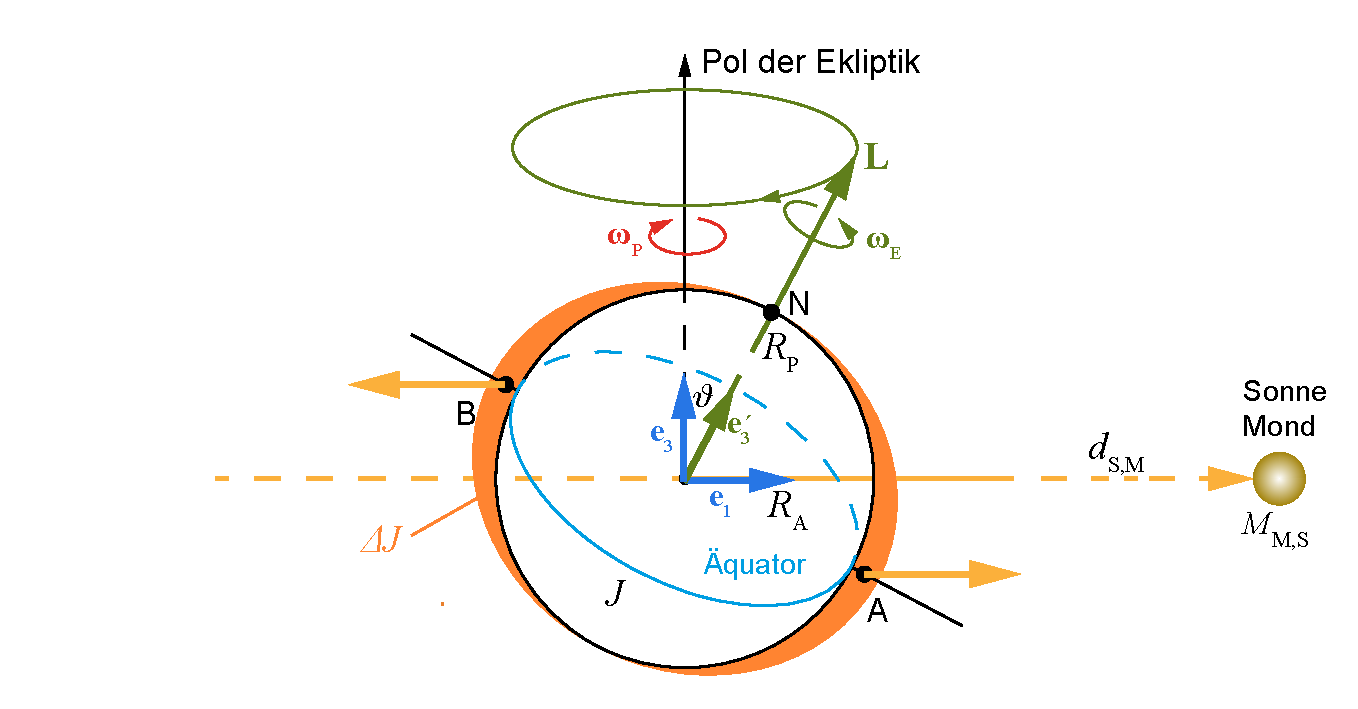
\includegraphics[width=\textwidth]{ErdPraezession01.pdf}
  \caption[Pr�zession der Erde durch Gezeitenkr�fte von Sonne und Mond.]{Pr�zession der Erde durch Gezeitenkr�fte von Sonne und Mond.}
    \label{abb:bew_Erdpraezession}
\end{figure}

Das von Sonne und Mond bewirkte Drehmoment auf die Erdachse (\figref{bew_Erdpraezession}) kann in guter N�herung wie folgt berechnet werden, siehe auch \cite{Bartelmann2015, Montenbruck2012} und \probref{bew_DrehmomentPraezErde}: \\
        \begin{align}
            \begin{split}
                \vec{M}_\text{S} &= \frac{3G\,m_\text{S}}{2{d_\text{S}}^3}\,\cos\vartheta\,\Delta J\,\lk \vecpeZ\times\veceZ \rk = C_\text{S}\,\lk \vecpeZ\times\veceZ \rk\,, \\
                \vec{M}_\text{M} &=  \frac{3G\,m_\text{M}}{2{d_\text{M}}^3}\,\cos\vartheta\,\Delta J\,\lk \vecpeZ\times\veceZ \rk = C_\text{M}\,\lk \vecpeZ\times\veceZ \rk \,. \label{eq:bew_ErdPraezess01}
            \end{split}
        \end{align}
Hierin sind $m_\text{S}, m_\text{M}$ die Massen von Sonne und Mond, $d_\text{S}, d_\text{M}$ die Abst�nde der Himmelsk�rper vom Erdmittelpunkt und $\vartheta$ der Neigungswinkel der Erdachse zur Bahn. $\vecpeZ$ ist der Achsenvektor im mitbewegten System der Erde und $\veceZ$ der Normalenvektor der \textit{Ekliptik} (Erdbahnebene)\index{Ekliptik}. Wir haben hierbei angenommen, dass der Mond sich ebenfalls in dieser Ebene bewegt. In \figref{bew_Erdpraezession} sind die Gezeitenkr�fte eingezeichnet, die auf die �quatorwulst wirken. Das resultierende Moment w�rde die Erdachse aufrichten, wenn die Erde kein rotierender Kreisel w�re.\\
Wie man in \eqref{eq:bew_ErdPraezess01} an der $d_\text{S,M}{}^{-3}$-Abh�ngigkeit erkennen kann, werden diese Drehmomente durch Gezeitenkr�fte (siehe \kap{bew_gezeiten}) hervorgerufen. In \probref{bew_DrehmomentPraezErde} werden wir das im Detail zeigen und auch \eqref{eq:bew_ErdPraezess01} herleiten. Wir wollen noch in sehr guter N�herung annehmen, dass die Figurenachse der Erde mit der Drehimpulsachse zusammenf�llt, dass also $ \vec{L} = L\,\vecpeZ$ gilt. Dann folgt aus der Bewegungsgleichung f�r den starren K�rper
        \begin{align}
            \frac{\D \vec{L}}{\D t} = \vec{M}_\text{M} + \vec{M}_\text{S} \label{eq:bew_ErdPraezess02}
        \end{align}
sofort eine Beziehung f�r das Betragsquadrat des Drehimpulses
        \begin{align}
           \frac{1}{2}\,\frac{\D L^2}{\D t} &= \vec{L}\,\frac{\D \vec{L}}{\D t} = L\,\vecpeZ\,\cdot\,\lk \vec{M}_\text{M} + \vec{M}_\text{S}\rk \approx L\,\underbrace{\vecpeZ\,\cdot\,\lk \vecpeZ\times \veceZ\rk\lk C_\text{S} + C_\text{M} \rk }_{\substack{=0}} \,. \label{eq:bew_ErdPraezess02a}
        \end{align}
Das hei�t, durch das Drehmoment der Gezeitenkr�fte kann sich
in unserem Modell nur die Richtung des Erddrehimpulses �ndern,
nicht aber sein Betrag.
Die Gezeitenkr�fte bewirken in unserem Fall des starren Rotationsellipsoiden also \emph{keine} Abbremsung
der Erdrotation, im Gegensatz zu einem anderen Modell einer teilweisen
nichtstarren Erde, das zum Effekt der Gezeitenreibung f�hrt (siehe auch Band II, Kapitel 3).\\
Wir wollen nun die Pr�zessionsfrequenz bestimmen. \\
Aus \eqref{eq:bew_ErdPraezess02} findet man mit $\vec{L} = L\,\vecpeZ$
        \begin{align*}
            \frac{\D \lk L\,\vecpeZ\rk}{\D t} &= J_3\, \omega_\text{E} \frac{\D \lk \vecpeZ\rk}{\D t} = L \vec{\omega}_\text{P} \times \vecpeZ = - L \vecpeZ \times \vec{\omega}_\text{P}  = -J \, \omega_\text{E} \, \omega_\text{P} \,\lk \vecpeZ \times \veceZ\rk \\
						&= \frac{3G\,\cos\vartheta\,\Delta J }{2}\lk \frac{m_\text{S}}{{d_\text{S}}^3}+\frac{m_\text{M}}{{d_\text{M}}^3}\rk \, \lk \vecpeZ\times \veceZ \rk \,.
 					\end {align*}
        \begin{align}
          \rightarrow \,\, \vec{\omega}_\text{P} &= - \underbrace{\frac{3G\,\cos\vartheta\,\Delta J }{2\, J_3\,\omega_\text{E}}\lk \frac{m_\text{S}}{{d_\text{S}}^3}+\frac{m_\text{M}}{{d_\text{M}}^3}\rk}_{= \left|\vec{\omega_\text{P}}\right| = \omega_\text{P}}\,\veceZ \label{eq:bew_ErdPraezess03}
        \end{align}
In \eqref{eq:bew_ErdPraezess03} erkennen wir $\omega_\text{P} = M/L$ aus \eqref{eq:bew_SchwererKr02} wieder.
Mit den bekannten Werten $\vartheta \approx \SI{23.45}{\degree}$, $m_\text{S} = \SI{1.98e30}{\kg}$, $m_\text{M} = \SI{7.35e22}{\kg}$, $d_\text{S} = \SI{1.49e11}{\metre}$, $d_\text{M} = \SI{3.84e8}{\metre}$ und $\omega_\text{E} = 2\pi/(\SI{86125}{\second})$ ergibt sich insgesamt 
        \begin{align*}
            \omega_\text{P} = \SI{7.94e-12}{\per\second} ~~~~ \text{oder} ~~~~ T_\text{P} = \frac{2\pi}{\omega_\text{P} } \approx 25\,100\,\text{Jahre}\,,
        \end{align*}
was sehr gut mit den astronomisch beobachteten 25\,800 Jahren �bereinstimmt.
Es sei bemerkt, dass die Beitr�ge von Mond und Sonne sich wie 2.2 : 1 verhalten. Das gleiche Verh�ltnis hatten wir bei den Gezeiten gefunden, was nicht verwunderlich ist, da f�r das Drehmoment der Pr�zession ja die Gezeitenkr�fte verantwortlich sind. F�r eine vertiefte Betrachtung empfehlen wir auch die Ref. \cite{Rainey2022}, die auch die Konsequenzen dieser Pr�zession der Erdachse auf das Langzeitverhalten unseres Klimas beleuchtet. Wir werden das ebenfalls mit einer etwas vereinfachten Methode im Kapitel Himmelsmechanik im Band II, Kapitel 3 tun. 
Eine genauere Untersuchung der Bewegung der Erdachse zeigt im �brigen, dass diese auch noch kleinere und kurzperiodischere (ca.\ 18--19 Jahre) nick�hnliche Bewegungen macht, die als 
\emph{astronomische} Nutation\index{Nutation!astronomische}
bezeichnet werden. 
Es sei darauf hingewiesen, dass der Begriff der astronomischen
Nutation nicht identisch ist mit dem in \autoref{kap:bew_starrer_koerper}
definierten Begriff der Nutation in der Kreiseltheorie.
Die astronomische Nutation als relativ schnell schwankender,
aber viel kleinerer Teil der Pr�zession der Erdachse ist also
selbst eine Pr�zession, die vor allem von der Pr�zession
der Mondbahn hervorgerufen wird.%
\footnote{Auch das Mond-Erde-System kann man als Kreisel betrachten,
der im Schwerefeld der Sonne pr�zediert.}
Als Folge dieser beiden genannten Richtungs�nderungen
der Erdachse ver�ndern sich nat�rlich auch die Koordinaten
der Sterne �ber die Zeit. Die Pr�zession der Erde war schon mehr als anderthalbtausend Jahre bekannt, bevor die astronomische Nutation der Erdachse 1728 von James Bradley\footnote{James Bradley\indexp{Bradley, James} (1693--1762) war ein englischer Astronom. Er gilt als einer der Pioniere der Astrometrie\index{Astrometrie} und wies die Bewegung der Erde um die Sonne durch die j�hrliche Aberration\index{Aberration} der Gestirne nach.} entdeckt wurde. Die Ursache dieser astronomischen Nutation konnte man dann aber erst 20 Jahre sp�ter auf Basis der oben beschriebenen Theorie des starren K�rpers erkl�ren.

\subsection{Trebuchet}\label{kap:bew_trebuchet}

\begin{figure}
\includegraphics[width=\textwidth]{Blide01.pdf}
\caption[Mittelalterliche Wurfmaschine und Prinzip der Funktionsweise.]{Nachbau (links) und Funktionsweise (rechts)  einer mittelalterlichen Steinschleuder (Trebuchet, Blide).}\label{abb:bew_Blide01}
\end{figure}

Zum Schluss des Kapitels Physik der Bewegung von K�rpern wollen wir uns noch ein besonderes Highlight g�nnen und eine mittelalterliche Steinschleuder behandeln.
Hierbei k�nnen wir fast alles Gelernte anwenden, insbesondere die Erhaltungss�tze, Zwangsbedingungen, Lagrange-Multiplikatoren und Lagrange-Gleichungen erster und zweiter Art, sowie numerische L�sungen mit ODE- und DAE-Solvern von \matlab.\\
Die Steinschleuder (\figref{bew_Blide01}) war im Mittelalter eine der gr��ten und zugleich genauesten Wurfwaffen mit ungeheuerlicher Durchschlagskraft und relativ gro�er Reichweite. 
H�ufig wurden diese auch als Tribok, Trebuchet (vom franz�sischen \textit{tr�buchet} \textit{Dreifu�}) oder Blide (aus dem Mittelhochdeutschen) bezeichnet. 
Sie funktioniert nach dem Hebelarmprinzip, bei dem ein gro�es Gegengewicht auf der kurzen Armseite f�r die Beschleunigung des kleineren Gewichts an der langen Armseite sorgt. 
Das Verh�ltnis der Hebelarme lag typischerweise zwischen 1:3 und 1:6. 
Au�erdem lassen sich Bauformen mit starrem und beweglichem Gegengewicht unterscheiden. 
Bei der Bauform mit beweglichem Gegengewicht am kurzen Armende gibt es wiederum zwei verschiedene Ausf�hrungen. 
Am h�ufigsten verwendet wird jene, bei der das Gegengewicht an einem Pendelarm nach unten h�ngt
und der Kreisbewegung des kurzen Arms aufgrund der Tr�gheit nur teilweise folgt.
Es pendelt relativ zur Ausgangslage um einen Winkel -- zun�chst nach innen, dann nach au�en. 
Diese Pendelbewegung hat (wie wir sp�ter noch sehen werden)
einen erheblichen Einfluss auf die Effizienz bei der Umwandlung
potentieller Energie der Gegenmasse in kinetische Energie des Wurfgeschosses. 
Bei der anderen Ausf�hrung des Trebuchet mit beweglicher Gegenmasse gleitet die gro�e Gegenmasse entlang einer F�hrung vertikal nach unten und ist �ber ein Gelenk mit dem Wurfarm verbunden (siehe \probref{bew_Trebuchet} und \mscr{} \mlbewref{TrebuchetSim01.m}).\\
Ein Gef�hl f�r die Dimensionen dieser Meisterwerke der mittelalterlichen Mechanik bekommt man, wenn man ber�cksichtigt, dass typische Gegenmassen zwischen \num{10} und \SI{20}{\tonne}  und  Wurfgeschosse zwischen 50 und $\SI{500}{\kg}$ hatten \cite{Chevedden1995}.
Weitere Hinweise finden sich in \cite{Denny2005, Chevedden1995, Siano2013,Constans2013, Constans2017}, die zum Teil auch die Grundlage f�r die nachfolgenden Betrachtungen waren und weitere Details f�r Vertiefung bieten. \\
F�r die Modellierung benutzen wir \figref{bew_TrebNaeherung4}. 
Das Trebuchet hat einen festen Drehpunkt in der H�he $h$ und ein Hebelverh�ltnis des Balken $B/b$ mit dem Massenverh�ltnis $m_\text{B}/m_\text{b}$.

Ab hier verwenden wir etwas unphysikalisch die Bezeichnungen \anf{Gegengmasse} und
\anf{Wurfgeschoss} f�r die bewegten Massen $m_\text{G}$ und $m_\text{W}$. Diese h�ngen jeweils an Seilen der L�nge $l_\text{G}$ \bzw $l_\text{W}$. 
F�r den Lagrange-Formalismus ist es sinnvoll, die Winkel $\gamma$, $\beta$ und $\delta$ als verallgemeinerte Koordinaten zu w�hlen. 

\begin{figure}
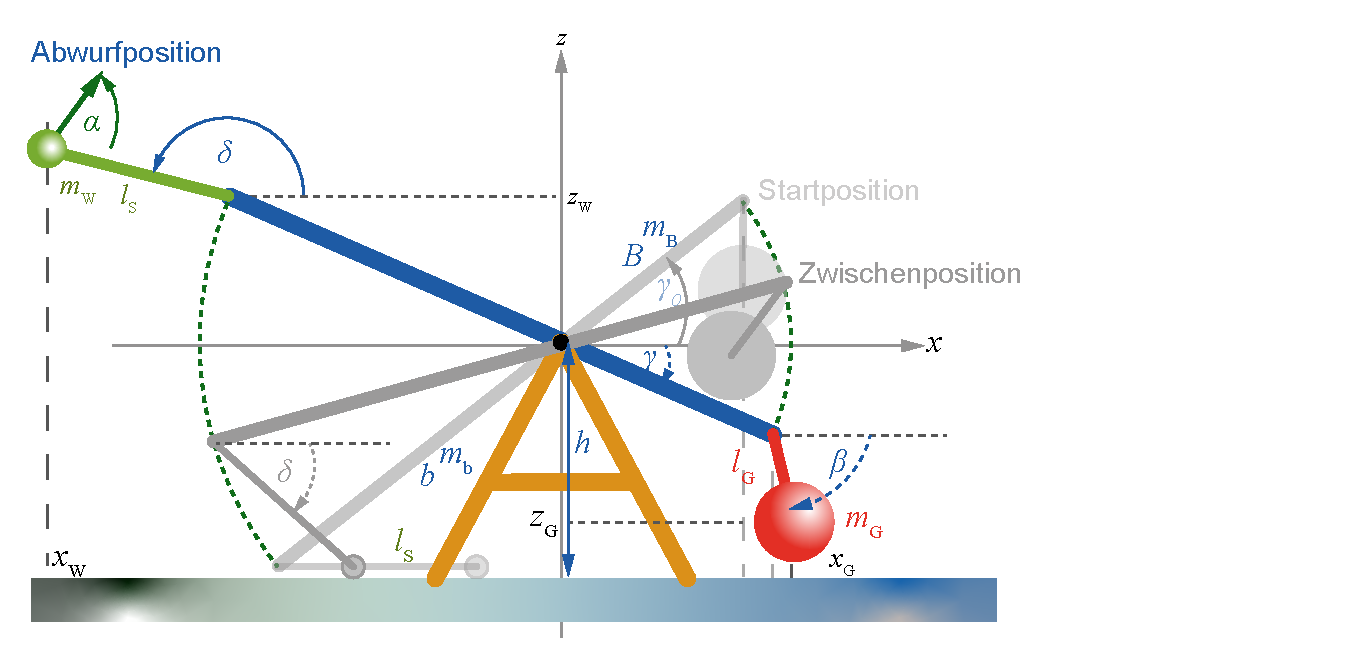
\includegraphics[width=\textwidth]{TrebNaeherung4.pdf}
\caption[Geometrie und physikalische Gr��en der Bestandteile.]{Geometrie und physikalische Gr��en der Bestandteile einer mittelalterlichen Wurfmaschine (Trebuchet, Blide).
Man beachte, dass alle Winkel au�er $\alpha$ im mathematisch positiven Drehsinn gegen die $x$-Achse als Bezugsachse definiert sind.}\label{abb:bew_TrebNaeherung4}
\end{figure}  % Negative Winkel sind im Bild als gestrichene B�gen gekennzeichnet.

Wir k�nnen nun den Wurfprozess in folgende drei Phasen unterteilen:
\begin{enumerate} [a)]
\item %a 
$0 < t \leq t_1$ Phase 1, Schleifphase\\
Das Wurfgeschoss wird beim Losl�sen der Masse $m_\text{G}$ zun�chst beschleunigt in Richtung $-\veceX$ gezogen. 
Da das Wurfgeschoss auf dem Boden aufliegt, m�ssen wir die Zwangsbedingung $z_\text{m}=-h$ beachten. 
Der Zeitpunkt $t_1$ ist dann der Moment, in dem das Wurfgeschoss gerade abhebt,
\dh zu dem die wirkende Zwangskraft Null wird.
Zu dieser Zeit entspricht die Beschleunigung des Wurfgeschosses in $z$-Richtung genau $m_\text{W} g$. 
Wir k�nnten f�r diesen Teilabschnitt ausschlie�lich mit verallgemeinerten Koordinaten $\beta$ und $\gamma$ arbeiten, indem wir die entsprechende Zwangsbedingung 
\begin{align}
	z_\text{m}=-h = - b\sin\gamma + l_\text{W}\sin\delta 
	\label{eq:bew_trebtheo01}
\end{align}
verarbeiten. 
Das f�hrt aber wegen der transzendenten Beziehungen in \eqref{eq:bew_trebtheo01}
auf sehr un�bersichtliche Bewegungsgleichungen, sodass wir auch f�r diese Phase
alle drei Winkel $\gamma$, $\delta$ und $\beta$ verwenden wollen. 
Die Zwangsbedingung ber�cksichtigen wir dann
bei der Anwendung der Methode der Lagrange-Multiplikatoren (\kap{bew_Lagrange_I}). 
Die Anfangsbedingungen sind durch $\beta_0 = \SI{-90}\degree$ und $\gamma_0$ gegeben, woraus au�erdem folgt, dass
\begin{align}
	-\delta_0 = \arcsin\lk \frac{h - b \sin\gamma_0}{l_\text{W}}\rk 
	\quad \text{und} \quad 
	h < b\,\sin\gamma_0 + l_\text{W}\,,
	\label{eq:bew_trebtheo01a}
\end{align} 
da sonst das Wurfgeschoss nicht wie gefordert auf dem Boden aufliegt.
Das Seil mit der L�nge $l_\text{W}$ wird dabei als gespannt angenommen.
\item %b 
$t_1<t<t_2$ Phase 2, Beschleunigungsphase nach oben\\
Das Wurfgeschoss hebt nun vom Boden ab ($z_\text{m}>0$), \dh es gibt nun keine Zwangsbedingungen mehr. 
Die drei Freiheitsgrade sind wieder durch die Winkel $\gamma$, $\delta$ und $\beta$ gegeben.
Die Anfangswerte sind durch die Endwerte von Phase 1 gegeben. %$\left[\beta(t_1), \gamma(t_1) ~\text{und}~ \delta(t_1)\right]$ 
\item %c
$t>t_2$ Phase 3, Flugphase\\ 
Ab $t>t_2$ bewegt sich das Geschoss frei auf der Wurfbahn des schr�gen Wurfs. 
Phase 3 wird dadurch ausgel�st, dass 
das Seil der Wurfschleuder gestoppt wird und damit das Wurfgeschoss in den schiefen Wurf (mit Luftreibung) �bergeht. 
Den entsprechenden (optimalen) Winkel zur Zeit $t_2$ bezeichnen wir mit $\gamma_2$. 
Die verallgemeinerten Koordinaten f�r diese Phase sind sinnvollerweise die kartesischen Koordinaten $x_\text{W}$ und $z_\text{m}$ mit den Bewegungsgleichungen
\begin{align}
	\ddot{x}_\text{W}+\eta \, \dot{x}_\text{W}\sqrt{\dot{x}_\text{W}{}^2+\dot{z}_\text{m}{}^2} &= \,0 \nonumber \\
	\ddot{z}_\text{m}+\eta \, \dot{z}_\text{m}\sqrt{\dot{x}_\text{W}{}^2+\dot{z}_\text{m}{}^2} \,+ \,g &= \,0 \,, \label{eq:bew_trebtheo02}
\end{align}
wobei $\eta$ der Reibungskoeffizient \[\eta= \frac{1}{2} \, c_\text{W} \, \frac{A_\text{W}} {m_\text{w}} \, \varrho_\text{L}\] ist. 
Hierin ist der Luftwiderstand $c_\text{W} \approx 0.45$, 
die Luftdichte $\varrho_\text{L}= \SI{1.3}{\kilogram\per\cubic\metre}$ 
und $A_\text{W}$ ist der Geschossquerschnitt,
der sich aus der Masse und der Dichte $\varrho_\text{W}$ des Geschosses
(bei einem Steingeschoss in etwa) $\varrho_\text{W}\approx \SI{2500}{\kilogram\per\cubic\metre}$
berechnen l�sst. 
Diese Phase soll hier nicht weiter betrachtet werden, da sie bereits ausf�hrlich in den �bungen zur Ballistik (�bungen \ref{prob:bew_Coriolis_II} bis \ref{prob:bew_Coriolis_IV}) untersucht worden ist. 
Die Anfangswerte sind durch die Endwerte von Phase 2 gegeben, n�mlich $x_\text{W}(t_2)$, $z_\text{m}(t_2)$ und 
\begin{equation}
v_\text{W} = \sqrt{\dot{x}_\text{W}(t_2)^2+\dot{z}_\text{m}(t_2)^2}\,. 
\label{eq:bew_trebtheo02a}
\end{equation}
Der Abwurfwinkel ist gegeben durch
\begin{align}
 	\alpha_\text{W} = \arctan \lk\frac{\dot{z}_\text{m}(t_2)}{\dot{x}_\text{W}(t_2)}\rk. \label{eq:bew_treb03a}
\end{align}
Mit der Zeit $t_2$ f�r die maximale Wurfweite
hat man auch $\gamma(t_2)=\gamma_2$, $\beta(t_2)$ und $\delta(t_2)$ bestimmt
und damit die Stellung des Trebuchet beim Ausl�sen des Wurfgeschosses. Zu diesem Zeitpunkt soll die Gegenmasse noch nicht den Boden erreicht haben.
\end{enumerate}
F�r die numerische Auswertung und Simulation wollen wir die in Tabelle \ref{tab:bew_trebuchet_01} angegebenen Parameter f�r das Trebuchet benutzen: \\

\begin{table}[h]
\centering
\begin{tabular}{ l C{1cm} C{1.5cm} C{1.5cm} }
\hline
  \rule{0pt}{2pt} & &  & \\
  &  & Fall A & Fall B\\
  \rule{0pt}{2pt} & &  & \\
\hline
  \rule{0pt}{9pt}%
  Balkenl�nge Gegenmasse [\si\metre] & $B$ &  4 &   3\\
  Balkenl�nge Wurfgeschoss [\si\metre] & $b$ & 12 & 15 \\
  L�nge Seil Gegenmasse  [\si\metre] & $l_\text{G}$ &  3 & 1.5 \\
  L�nge Seil Wurfgeschoss  [\si\metre] & $l_\text{S}$ &  8 & 5 \\
  H�he Balkendrehpunkt     [\si\metre] & $h$ & 10 & 10 \\
\hline
  \rule{0pt}{9pt}%
  Gegenmasse [\si\kilogram] & $m_\text{G}$ & 10000 & 15000 \\
  Masse Wurfgeschoss [\si\kilogram] & $m_\text{w}$ & 100 & 50 \\
  Masse Balken       [\si\kilogram] & $m_\text{T}$ & $\approx 1040$ & $\approx 2160$ \\
  \rule{0pt}{9pt}%
  Masse Balken pro L�nge [\si{\kilogram\per\metre}] & $\frac{\D m}{\D z}$ & $\approx 65$ & $\approx 120$ \\
  %\rule{0pt}{2pt} & &  & \\
\hline
  \rule{0pt}{9pt}%
  %Anfangswerte f�r Winkel: &  &  &  \\
  Balkenwinkel & $\gamma_0$ & $55\degree$ & $40\degree$ \\
  Pendelwinkel & $\beta_0$ & $-90\degree$ & $-90\degree$\\
  Seilwinkel der Schleuder& $\delta_0$ & $-1.2\degree$ & $-4.1\degree$\\
\hline
\end{tabular} 
\smallskip \\
\smallskip
\caption[Zwei typische Dimensionierungen einer mittelalterlichen Wurfschleuder.]{Zwei typische Dimensionierungen einer mittelalterlichen Wurfschleuder (Blide, Trebuchet).} \label{tab:bew_trebuchet_01}
\end{table}

Wie bereits an der Geometrie in \figref{bew_TrebNaeherung4} erkennbar, ist das System relativ komplex.
Wir werden uns deshalb die Dynamik des Trebuchet Schritt f�r Schritt erschlie�en.
Dabei starten wir mit einem sehr einfachen Modell und verfeinern dieses immer weiter.
Dieses Vorgehen haben wir schon mehrfach realisiert (\ua bei den verschiedenen Kreiselvarianten in \kap{bew_Lagrange_StarrerK} und \ref{kap:bew_SchwererSymmKr}) und ist immer dann zu empfehlen, um die anzuwendenden Prinzipien besser sichtbar werden zu lassen. Dar�ber hinaus erlaubt dieses Vorgehen, bei jeder Modellverfeinerung den Grenzfall des einfacheren vorherigen Modell �berpr�fen zu k�nnen.\\
Wir k�nnen die verallgemeinerten Koordinaten und Geschwindigkeiten aufschreiben, die wir zur Berechnung der Lagrange-Funktion ben�tigen. 
Diese sind f�r alle Modelle g�ltig und die entsprechenden Beziehungen k�nnen aus \figref{bew_TrebNaeherung4} abgeleitet werden.
Bei den verschiedenen behandelten N�herungen werden dann jeweils bestimmte Parameter vernachl�ssigt wie \zb $l_\text{W}$ und $l_\text{G}$. 
Wir finden f�r das Wurfgeschoss folgende Bewegungsgleichungen:
\begin{align}
	\begin{pmatrix} x_\text{W} \\ z_\text{m}  \end{pmatrix} &=
	\begin{pmatrix} -b\,\cos\gamma + l_\text{W}\,\cos\delta \\ -b\,\sin\gamma + l_\text{W}\,\sin\delta 	\end{pmatrix}, \nonumber \\
	\begin{pmatrix} \dot{x}_\text{W} \\ \dot{z}_\text{m}  \end{pmatrix} &=
	\begin{pmatrix} +b\,\dot{\gamma}\,\sin\gamma - l_\text{W}\,\dot{\delta}\,\sin\delta \\ -b\,\dot{\gamma}\,\cos\gamma + l_\text{W}\,\dot{\delta}\,\cos\delta \end{pmatrix}\,,
	\label{eq:bew_trebkoord01}
\end{align}
und f�r die Gegenmasse:
\begin{align}
	\begin{pmatrix} x_\text{G} \\ z_\text{G} 	\end{pmatrix} &=
	\begin{pmatrix} +B\,\cos\gamma + l_\text{G}\,\cos\beta \\ B\,\sin\gamma + l_\text{G}\,\sin\beta 	\end{pmatrix} \,, \nonumber \\
	\begin{pmatrix} \dot{x}_\text{G} \\ \dot{z}_\text{G} 	\end{pmatrix} &=
	\begin{pmatrix} -B\,\dot{\gamma}\,\sin\gamma - l_\text{G}\,\dot{\beta}\,\sin\beta \\ +B\,\dot{\gamma}\,\cos\gamma + l_\text{G}\,\dot{\beta}\,\cos\beta \end{pmatrix}\,.
	\label{eq:bew_trebkoord02}
\end{align}
Damit lassen sich die Lagrange-Funktionen und die Lagrange-Gleichungen in den drei generalisierten Koordinaten aufschreiben. 
Wer sich etwas Schreibarbeit sparen m�chte, nutzt dazu die Symbolic Math Toolbox (siehe \mscr{} \mlbewref{TrebSimulation.m}).\\
F�r die Lagrange-Funktion werden die kinetischen und potentiellen Energien der drei K�rper (Balken, Gegenmasse und Wurfgeschoss) addiert, also
\begin{align}
	\mathcal{L} &= T_\text{B} + T_\text{G} + T_\text{W} - f_\text{B} - f_\text{G} -f_\text{W} \,.\label{eq:bew_trebG00}
\end{align}
F�r den Balken gilt
\begin{align}
	  T_\text{B} &=  \frac{J_B}{2} \dot{\gamma}^2 \; , \nonumber \\
	  f_\text{B} &=  -\frac{1}{2}\,m_\text{T}\,g\,(b-B)\,\sin\gamma \;, \label{eq:bew_trebG01}
\end{align}
worin $J_\text{B} = \frac{1}{3}\,m_\text{T}\,\lk \frac{B^3+b^3}{B+b} \rk$ das Tr�gheitsmoment%
\footnote{Der Begriff Tr�gheitsmoment wurde genauer in \kapitel{bew_StarrerK_kin_Energie} eingef�hrt.
Hier gen�gt es, das Tr�gheitsmoment als die Summe aller Produkte der bewegten Massen mit den jeweiligen Quadraten der Abst�nde zur Drehachse zu definieren.}
eines homogenen Balkens mit der Gesamtmasse $m_\text{T} = m_\text{B}+m_\text{b}$ ist. 
F�r die Gegenmasse gilt
\begin{align}
	  T_\text{G} &=  \frac{m_\text{G}}{2} \lek B^2\,\dot{\gamma}^2 + 2 l_\text{G}\,B\,\dot{\gamma}\,\dot{\beta}\,\cos\lk\gamma-\beta\rk + l_\text{G}{}^2\,\dot{\beta}^2\rek \; , \nonumber \\
	  f_\text{G} &=  m_\text{G}\,g\, \lek  B\,\sin\gamma + l_\text{G}\,\sin\beta \rek
	  \label{eq:bew_trebG02}
\end{align}
und analog f�r das Wurfgeschoss
\begin{align}
	  T_\text{W} &=  \frac{m_\text{W}}{2} \lek b^2\,\dot{\gamma}^2 - 2 l_\text{W}\,b\,\dot{\gamma}\,\dot{\delta}\,\cos\lk\gamma-\delta\rk + l_\text{W}{}^2\,\dot{\delta}^2\rek \; , \nonumber \\
	  f_\text{W} &=  m_\text{W}\,g\, \lek -b\,\sin\gamma + l_\text{W}\,\sin\delta \rek \,. \label{eq:bew_trebG03}
\end{align}
Diese Terme k�nnen wir nun in \eqref{eq:bew_trebG00} einsetzen und erhalten nach etwas Algebra und Benutzung der Additionstheoreme f�r Winkelfunktionen
\begin{align}
	 \mathcal{L}  &= T_\text{treb} - f_\text{treb}  \nonumber \\
	 \text{mit} \quad 
	 T_\text{treb} &= \frac{J_0}{2}\,\dot{\gamma}^2\, + \frac{J_\text{G}}{2}\,\dot{\beta}^2 + \frac{J_\text{W}}{2}\,\dot{\delta}^2 + \ldots\nonumber \\
	              &~+ J_\text{BG}\,\dot{\gamma}\,\dot{\beta}\,\cos\lk\gamma-\beta\rk - J_\text{bW}\,\dot{\gamma}\,\dot{\delta}\,\cos\lk\gamma-\delta\rk\,,\nonumber \\
	f_\text{treb} &= f_0\,\sin\gamma + m_\text{G}\,l_\text{G}\,g\,\sin\beta + m_\text{w}\,l_\text{W}\,g\,\sin\delta\,. \label{eq:bew_trebG04}
\end{align}
Hier haben wir zur Abk�rzung eingef�hrt:
\begin{align}
 f_0 &= g \lek m_\text{G}\,B - m_\text{w}\,b - \frac{1}{2}m_\text{T}\lk b-B\rk \rek \nonumber \\
 J_0 &= m_\text{W}\,b^2 + m_\text{G}\,B^2+J_\text{B} \nonumber \\
 J_\text{G} &= m_\text{G}\,l_\text{G}{}^2 \nonumber \\
 J_\text{W} &= m_\text{W}\,l_\text{W}{}^2 \nonumber \\
 J_\text{BG} &= m_\text{G}\,B\,l_\text{G} \nonumber \\
 J_\text{bW} &= m_\text{W}\,b\,l_\text{W}\,. \label{eq:bew_trebG04a}
\end{align}
Die $J_i$ und $f_0$ sind Konstanten, die allein durch die Geometrie und die Massen des Trebuchet bestimmt sind.
Der Vorteil dieser Notation ist, dass mit $J_0$ und $f_0$ Grundelemente gegeben sind, die in der Lagrange-Funktion der komplexeren Trebuchet-Designs erhalten bleiben und durch Zusatzterme erweitert werden. \\

\subsubsection{Trebuchet als Wippe (Modell 1)}

\begin{figure}
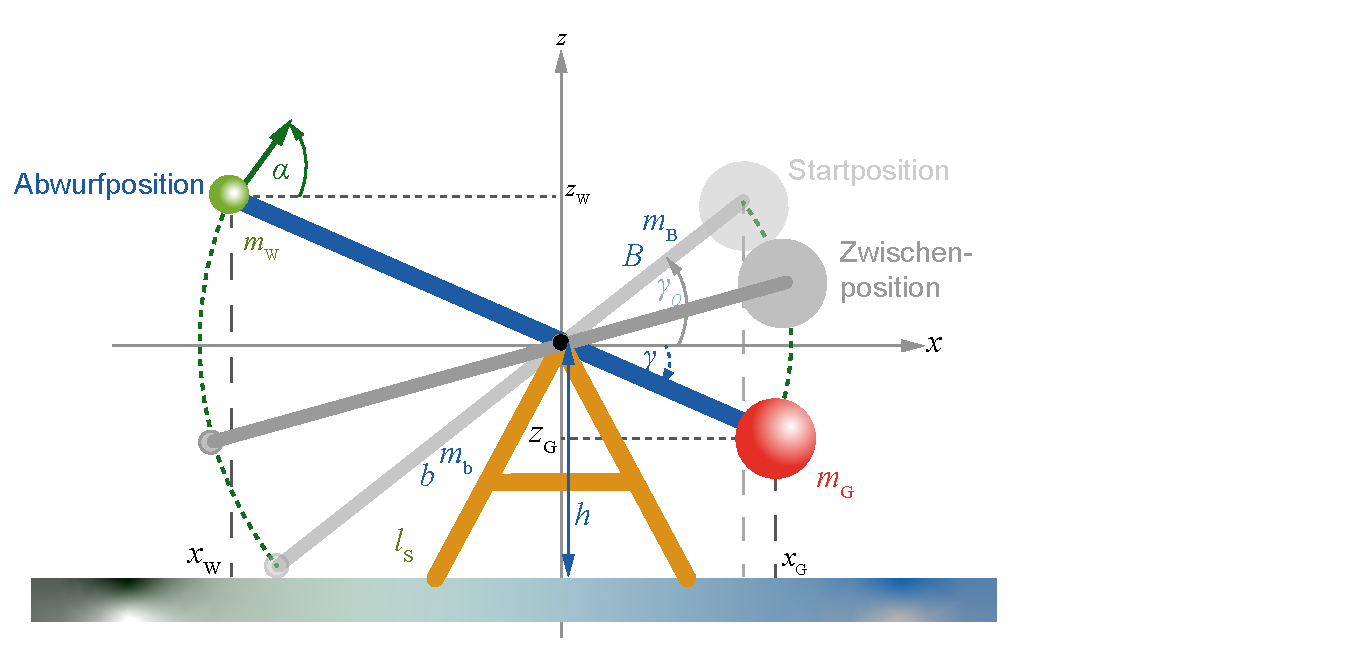
\includegraphics[width=\textwidth]{TrebNaeherung1.pdf}
\caption[Trebuchet als Wippe.]{Trebuchet als Wippe (Modell 1).}\label{abb:bew_TrebNaeherung1}
\end{figure}

Wir beginnen mit dem einfachsten Modell des Trebuchet als Wippe (\figref{bew_TrebNaeherung1}), also der Urform einer Steinschleuder, wie sie schon in der Antike bekannt war. 
Bei diesem System ist $l_\text{W} = 0$ und $l_\text{G}=0$. 
Wir haben also f�r dieses einfache Modell als generalisierte Koordinate nur den Winkel $\gamma$. 
Die Lagrange-Funktion ist dann gegeben durch
\begin{align}
		\mathcal{L}_{\uproman{1}} &= \frac{J_0}{2}\,\dot{\gamma}^2\, - \,f_0\sin\gamma \,. \label{eq:bew_treb01}
\end{align}
Da keine Zwangsbedingungen vorliegen, gibt es keine Phase 1. 
F�r Phase 2 l�sst sich folgende Bewegungsgleichung aus der Lagrange-Gleichung ableiten:
\begin{align}
		\frac{\D}{\D t}\frac{\d\mathcal{L}_{\uproman{1}}}{\d\dot{\gamma}}-\frac{\d\mathcal{L}_{\uproman{1}}}{\d\gamma} = 0 = J_0\,\ddot{\gamma} + f_0\,\cos\gamma \,. \label{eq:bew_treb02}
	\end{align}
Wie bereits erw�hnt wird Phase 3 dadurch ausgel�st, dass bei einem bestimmten (optimalen) Winkel $\gamma_2$ zur Zeit $t_2$ die Verbindung von Geschoss und Trebuchet (Schleudersack) gel�st wird und damit das Wurfgeschoss in den schr�gen Wurf �bergeht.
Wir wollen annehmen, dass dies bei demjenigen Winkel $\gamma_2$ erfolgt, f�r den die Wurfweite maximal ist.
Da beim schr�gen Wurf die Wurfweite sowohl von der Anfangsgeschwindigkeit als auch dem Abwurfwinkel abh�ngt, muss man also f�r verschiedene $t_2$ den Winkel $\alpha_\text{W}$ und die Geschwindigkeit 
$v_\text{W}$ \eqref{eq:bew_trebtheo02a} aus den Bewegungsgleichungen \eqref{eq:bew_trebtheo02} berechnen und daraus die erzielbare Wurfweite $W$ bestimmen.
Wir k�nnen das numerisch tun oder aber unsere analytischen Betrachtungen nutzen.
F�r vernachl�ssigbare Reibung lautet die Gleichung f�r die Reichweite bei einem schiefen Wurf mit einer Anfangsh�he $z_\text{W}(t_2) = z_\text{W2}$ und einem Abwurfwinkel $\alpha_\text{W}$
		\begin{align}
				W = \frac{v_2}{g} \cos\alpha_\text{W} \lk v_2\,\sin\alpha_\text{W} + \sqrt{{v}_2{}^2 \,(\sin\alpha_\text{W})^2 + 2\,g\,z_\text{W2}}\rk \,. \label{eq:bew_treb03}
		\end{align}
Mit dem so bestimmten $\alpha_\text{W}$ f�r die maximale Wurfweite findet man die Stellung des Trebuchet beim Ausl�sen des Wurfgeschosses.
Die entsprechende Dynamik ist in \figref{bew_TrebErgebnis1b} gezeigt (siehe \mscr{} \mlbewref{TrebSimulation.m}).
Wie man erkennt, ist die Energieumwandlung bei diesem System nicht optimal, ein erheblicher Teil der potentiellen Energie der Gegenmasse geht in kinetische Energie derselben �ber (vor allem durch einen Impuls in $x$-Richtung).
Man erzielt mit diesem System nur Reichweiten geringer als $\SI{100}{\metre}$.
Au�erdem wird ersichtlich, dass die Reichweite relativ kritisch vom Ausl�sezeitpunkt $t_2$ abh�ngt.\\

\begin{figure}
\begin{minipage}{\textwidth}
\leftfigure{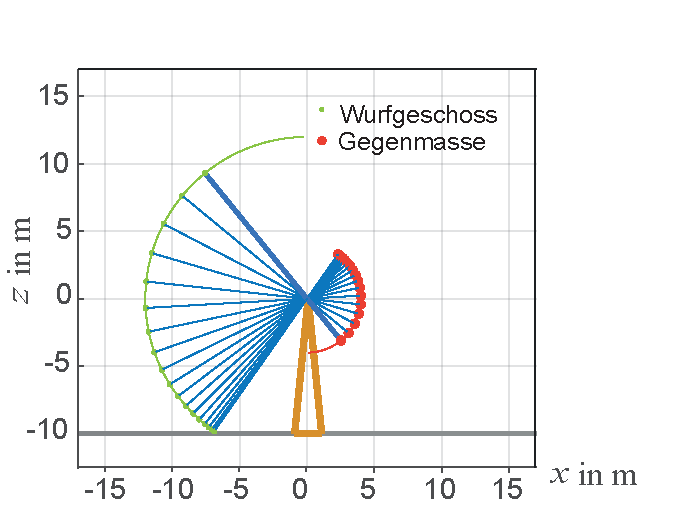
\includegraphics[width=0.5\textwidth]{TrebSim01b.pdf}}%
\hspace{\fill}
\rightfigure{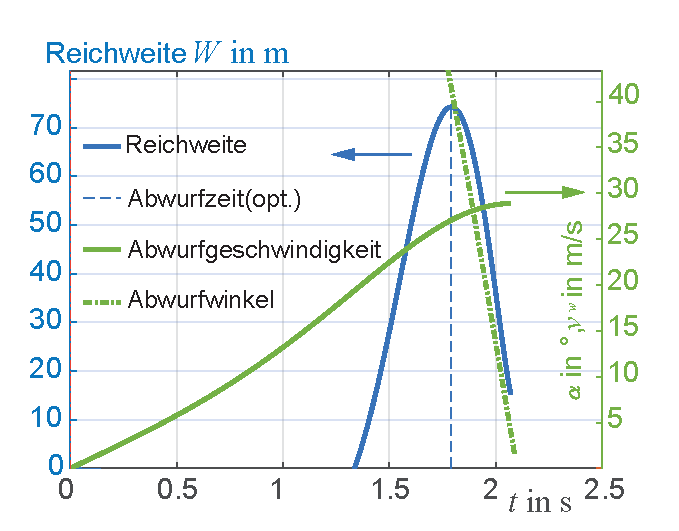
\includegraphics[width=0.5\textwidth]{TrebSim01a.pdf}}
\leftcaption[Dynamik der einfachen Steinschleuder.]{Dynamik der einfachen Steinschleuder (Modell 1).} \label{abb:bew_TrebErgebnis1b}
\rightcaption[Reichweite der einfachen Steinschleuder.]{Reichweite der einfachen Steinschleuder (Modell 1).} \label{abb:bew_TrebErgebnis1a}
\end{minipage}
\end{figure}

Wir k�nnen nun noch (und auch f�r alle folgenden Trebuchet-Modelle in gleicher Form) zwei Effizienzparameter definieren.
Die \emph{Reichweiteneffizienz}:
	\begin{align}
		\epsilon_\text{W} &= \frac{W}{W_\text{max}} \nonumber \\
		\text{mit} \quad 
		W_\text{max} &= \frac{2 \Delta U}{m_\text{W}\,g } \sqrt{\frac{z_\text{W}(t_2)}{\Delta U}\,m_\text{W}\,g+1} \nonumber \\
		\text{und} \quad 
		\Delta U &= -\lek U(t_2)-U(t_0)\rek \,.\label{eq:bew_treb04a}
	\end{align}
Dabei haben wir angenommen, dass alle \anf{freiwerdende} Energie 
vollst�ndig in kinetische Energie des Wurfgeschosses gewandelt wird.
Die Verringerung der potentiellen Energie der Gegenmasse 
abz�glich der Zunahme der potentiellen Energie von Balken und Wurfgeschoss
werden somit in einen optimalen Wurf umgesetzt.\\
Als zweiten Effizienzparameter definieren wir die 
\emph{Umwandlungseffizienz der potentiellen Energie} der Gegenmasse
\begin{align}
	\epsilon_\text{T} = \frac{T_\text{W}(t_2)}{\Delta U} \,, \label{eq:bew_treb04b}
\end{align}
worin $T_\text{W}(t_2)$ die kinetische Energie des Wurfgeschosses zum Zeitpunkt $t_2$ ist.
F�r die Werte aus Tabelle \ref{tab:bew_trebuchet_01} ergeben sich beispielhaft f�r Fall A folgende Effizienzparameter:
	\[ 
	\epsilon_\text{W} = 6.7 \% ~,~~\epsilon_\text{T} = 6.8 \% \,,
\]
was best�tigt, dass die Energieumwandlung bei diesem System suboptimal ist.

\begin{table}[h]
  \centering
  \begin{tabular}[h]{|l|c|r@.l|r@.l|r@.l|r@.l|r@.l|r|r|}
  \hline
%  \rule{0pt}{2pt}\\
  \phantom{x}&\phantom{x}&\multicolumn2{c|}{\phantom{x}}&\multicolumn2{c|}{\phantom{x}}&\multicolumn2{c|}{\phantom{x}}&\multicolumn2{c|}{\phantom{x}}&\multicolumn2{c|}{\phantom{x}}&\phantom{x}&\phantom{x}\\
  Parameter& ZB & \multicolumn2{c|}{$W$}   &  \multicolumn2{c|}{$t_\text{abw}$}    & \multicolumn2{c|}{$\alpha$}  & \multicolumn2{c|}{$v_\text{abw}$}    & \multicolumn2{c|}{$\epsilon_\text{T}$}   & $l_\text{G}$  & $l_\text{W}$  \\
  Einheit  &         &\multicolumn2{c|}{\si{\metre}} & \multicolumn2{c|}{\si{\second}} & \multicolumn2{c|}{\si{\degree}} & \multicolumn2{c|}{\si{\metre\per\second}} & \multicolumn2{c|}{\si{\%}} & q \si{\metre} & \si{\metre} \\
%  \rule{0pt}{2pt}\\
  \phantom{x}&\phantom{x}&\multicolumn2{c|}{\phantom{x}}&\multicolumn2{c|}{\phantom{x}}&\multicolumn2{c|}{\phantom{x}}&\multicolumn2{c|}{\phantom{x}}&\multicolumn2{c|}{\phantom{x}}&\phantom{x}&\phantom{x}\\
  \hline
  Modell 1 & nein    & 74&3& 1&78 & 40&4 & 27&0 &  6&8 & 0 & 0 \\
  Modell 2 & nein    &251&5& 1&60 & 29&6 & 53&4 & 23&7 & 3 & 0 \\
  Modell 3 & nein    &274&9& 1&90 & 42&3 & 51&9 & 24&1 & 0 & 8 \\
  Modell 4 & nein    &355&5& 1&66 & 37&3 & 60&0 & 28&7 & 3 & 8 \\
  Modell 4 & ja      &296&2& 1&58 & 35&1 & 55&4 & 19&6 & 3 & 8 \\
  FAT I    & nein    &432&9& 1&98 & 37&6 & 66&2 & 33&4 & 0 & 8 \\
  FAT II   & ja      &294&9& 2&18 & 36&1 & 55&0 & 29&5 & 0 & 8 \\
  \hline
  \end{tabular}
\caption[Vergleich der Reichweiten und Effizienzparameter verschiedener Trebuchet-Modelle.]{Vergleich der Reichweiten und Effizienzparameter verschiedener Trebuchet-Modelle. ZB steht f�r Zwangsbedingungen, FAT f�r \textit{Floating Arm Trebuchet}, siehe \probref{bew_Trebuchet}. Weitere Parameter: $h =\SI{10}{\metre}$, $m_\text{G} = \SI{10000}{\kilogram}$, $m_\text{W}= \SI{100}{\kilogram}$, $m_\text{T} = \SI{1040}{\kilogram}$, $B = \SI{4}{\metre}$, $b=\SI{12}{\metre}$.}
\label{tab:bew_trebuchet_02}
\end{table}


\subsubsection{Trebuchet mit pendelnder Gegenmasse (Modell 2)}

\begin{figure}
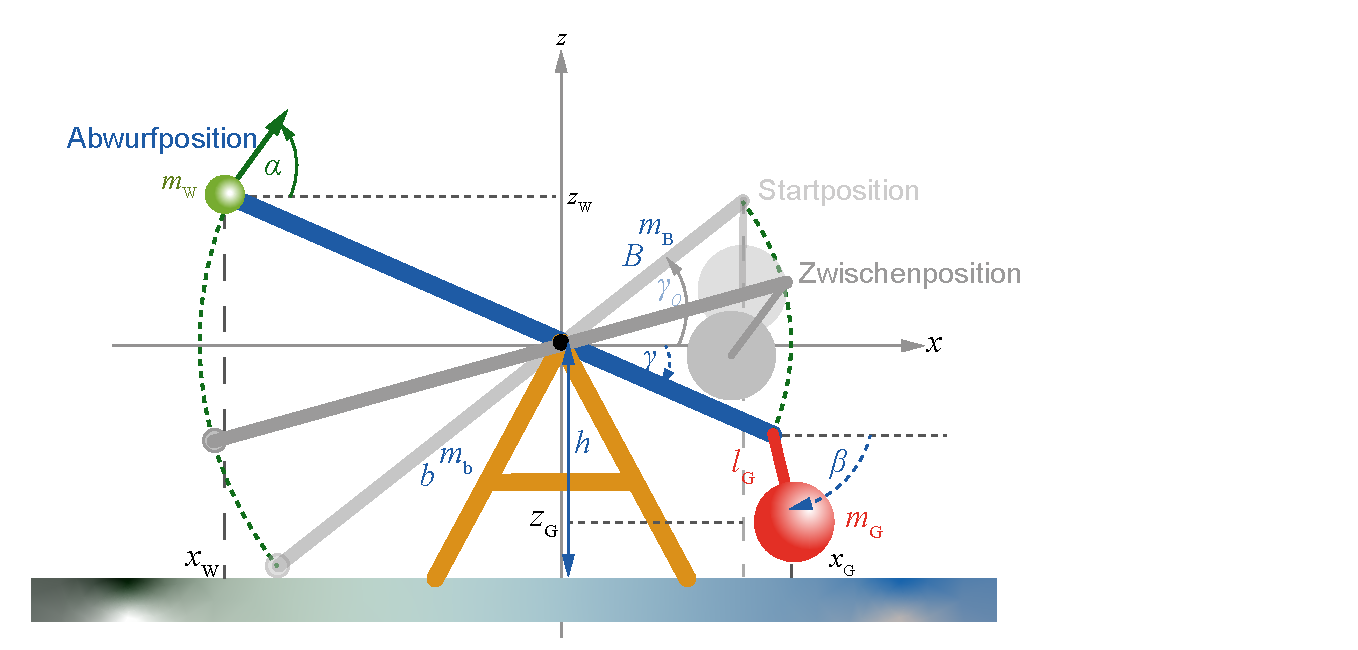
\includegraphics[width=\textwidth]{TrebNaeherung2.pdf}
\caption[Trebuchet mit pendelnder Gegenmasse.]{Trebuchet mit pendelnder Gegenmasse (Modell 2).}\label{abb:bew_TrebNaeherung2}
\end{figure}

Bei diesem Modell ist die Gegenmasse als Pendel aufgeh�ngt.
Dadurch kann die Reichweite deutlich gesteigert werden, da die Umwandlung von potentieller Energie der Gegenmasse in kinetische Energie (Impuls in $x$-Richtung) derselben durch die Pendelaufh�ngung deutlich reduziert wird. 
Die Lagrange-Funktion erweitert sich durch die neue Koordinate $\beta$ und ergibt sich nun aus \eqref{eq:bew_trebG04} zu
\begin{align}
		\mathcal{L}_{\uproman{2}} &= \mathcal{L}_{\uproman{1}} + \Delta\mathcal{L}_{\uproman{2}}  \nonumber \\
		&= \frac{J_0}{2}\,\dot{\gamma}^2 - f_0\,\sin\gamma + \ldots  \nonumber \\
		&~~+\frac{1}{2}\,J_\text{G}\,\dot{\beta}^2 + J_\text{BG}\,\dot{\gamma}\,\dot{\beta}\,\cos\lk \gamma-\beta \rk  - m_\text{G}\,l_\text{G}\,g\,\sin\beta \,. \label{eq:bew_treb05}
\end{align}
Daraus erhalten wir die Bewegungsgleichungen
\begin{align}
    \begin{split}
        J_0\,\ddot{\gamma}        &= -J_\text{BG}\,\ddot{\beta}\,\cos\lk \beta-\gamma\rk  + J_\text{BG}\,\dot{\beta}^2\,\sin\lk \beta-\gamma \rk - f_0\,\cos\gamma \,, \\
        J_\text{G}\,\ddot{\beta}  &= -J_\text{BG}\,\ddot{\gamma}\,\cos\lk \beta-\gamma\rk - J_\text{BG}\,\dot{\gamma}^2\,\sin\lk \beta-\gamma\rk - g\,m_\text{G}\,l_\text{G}\,\cos\beta \,. \label{eq:bew_treb06}
    \end{split}
\end{align}
Wir wollen dieses Differentialgleichungssystem wieder numerisch in \matlab{} integrieren.
Wir erkennen, dass man \eqref{eq:bew_treb06} in Matrixform schreiben kann.
Wir bringen dazu die Terme mit den zweiten Ableitungen auf die linke Seite und schreiben
\begin{align}
		\mathbb{M}(t,\vec{q}) \cdot \ddot{\vec{q}}  
			& = 
\begin{pmatrix}
J_0  & J_\text{BG}\,\cos\lk \beta-\gamma \rk \\
J_\text{BG}\,\cos\lk \beta-\gamma \rk & J_\text{G}
\end{pmatrix}
\begin{bmatrix}
		\ddot{\gamma} \\
		\ddot{\beta} 
\end{bmatrix} \nonumber \\
		&=
\begin{pmatrix}
+J_\text{BG}\,\dot{\beta}^2\,\sin\lk \beta-\gamma \rk - f_0\,\cos\gamma \\
-J_\text{BG}\,\dot{\gamma}^2\,\sin\lk \beta-\gamma \rk - g\,m_\text{G}\,l_\text{G}\,\cos\beta
\end{pmatrix}
\nonumber \\
&= \vec{F}(t,\vec{q},\dot{\vec{q}}) \, \label{eq:bew_treb07}
\end{align}
mit $\vec{q} =[\gamma,\beta]^\text{T}$, $\dot{\vec{q}} =[\dot{\gamma},\dot{\beta}]^\text{T}$ und $\ddot{\vec{q}} =[\ddot{\gamma},\ddot{\beta}]^\text{T}$. 
Der Vektor $\vec{F}(t,\vec{q},\dot{\vec{q}})$ hat die Dimension einer Kraft \bzw hier eines Drehmomentes. 
Die Elemente der Matrix auf der linken Seite sind Tr�gheitsmomente \bzw Massen, deshalb nennt man sie auch Massen- oder Tr�gheitsmoment-Matrix\index{Tr�gheitsmoment-Matrix}. 
F�r die numerische L�sung m�ssen wir diese aber noch etwas aufbereiten, da \matlab{} ja eine Routine zur Integration von Differentialgleichungssystemen erster Ordnung der Form $\dot{\vec{Y}} = \vec{f}_\text{g}(t, \vec{Y})$ zur Verf�gung stellt, in der die $Y_i(t)$ die gesuchten Funktionen sind. 
Wir setzen deshalb:
		\begin{align*} 
				\left[Y_1, Y_2,~ Y_3,~Y_4 \right]^\text{T} = \left[\gamma,~\dot{\gamma},~\beta,~\dot{\beta} \right]^\text{T} \,
		\end{align*}
und m�ssen dann auch die Massen-Matrix durch entsprechende Zeilen und Spalten erweitern.
Wir wollen diese auch weiterhin Massen-Matrix \cite{Wells1967, MATLABEx01}\index{Massen-Matrix} nennen.
Das DGL-System kann schlie�lich in folgender nun \matlab-kompatibler Form geschrieben werden:
\begin{align}
    \mathbb{M}(t,\vec{Y}) \cdot \dot{\vec{Y}}  &= 
    \begin{pmatrix}
	1 \quad\quad & 0  & 0 \quad\quad  & 0  \\
	0 & J_0 & 0    & J_\text{BG}\,\cos \lk Y_3-Y_1 \rk \\
	0 & 0 & 1    & 0  \\
	0 & J_\text{BG}\,\cos(Y_3-Y_1) & 0    & J_\text{G}
    \end{pmatrix} \cdot
    \begin{bmatrix}
	\dot{Y}_1 \\
	\dot{Y}_2 \\
	\dot{Y}_3 \\
	\dot{Y}_4 
    \end{bmatrix} \nonumber \\
    &= \begin{pmatrix}
	Y_2 \\
	J_\text{BG}\,Y_4^2\,\sin\lk Y_3-Y_1 \rk - f_0\,\cos Y_1\\
	Y_4 \\
	-J_\text{BG}\,Y_2^2\,\sin\lk Y_3-Y_1 \rk - g\,m_\text{G}\,l_\text{G}\,\cos Y_3 
    \end{pmatrix} \nonumber \\
    &= \vec{F}(t,\vec{Y},\dot{\vec{Y}}) \,. \label{eq:bew_treb08}
\end{align} 
Die Berechnung der L�sung des DGL-Systems mittels \matlab{} erfolgt gem�� der \kap{bew_matlab_dgl} beschriebenen Vorgehensweise zur L�sung von Gleichungssystemen der  Form $\D\vec{Y}/\D t = \vec{F}(t,\vec{Y},\dot{\vec{Y}})$. Hier wird beim Aufruf der \matlab{} Routine \odevf{} eine (gegebenenfalls parametrisierte) Matrix-Funktion $\mathbb{M} = \mathbb{M}(t,\vec{Y},P)$ �bergeben. Dabei ist $P$ ist eine vorteilhafte Struktur f�r den Parametersatz, in unserem Fall im Wesentlichen bestehend aus den geometrischen und physikalischen Parametern des Trebuchet.\\

\begin{figure}
\begin{minipage}{\textwidth}
\leftfigure{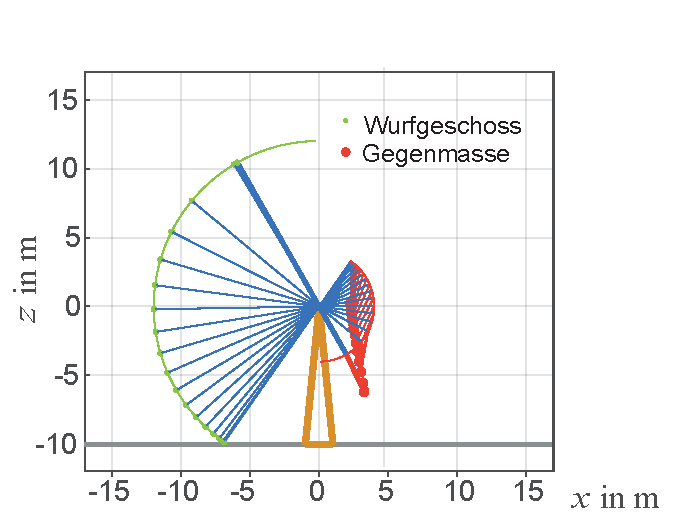
\includegraphics[width=0.5\textwidth]{TrebSim02b.pdf}}%
\hspace{\fill}
\rightfigure{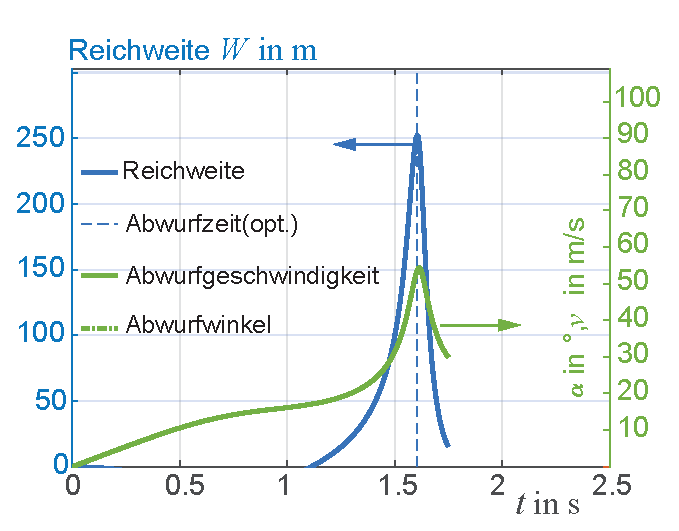
\includegraphics[width=0.5\textwidth]{TrebSim02a.pdf}}
\leftcaption[Dynamik eines Trebuchet mit pendelnder Gegenmasse.]{Dynamik eines Trebuchet mit pendelnder Gegenmasse (Modell 2).} \label{abb:bew_TrebErgebnis2a}
\rightcaption[Reichweite eines Trebuchet mit pendelnder Gegenmasse.]{Reichweite eines Trebuchet mit pendelnder Gegenmasse (Modell 2).} \label{abb:bew_TrebErgebnis2b}
\end{minipage}
\end{figure}

Die Rechnungen sind im Detail im  \mscr{} \mlbewref{TrebSimulation.m} ausgef�hrt,
die wesentlichen Ergebnisse sind in den \figref{bew_TrebErgebnis2a}
und \figref{bew_TrebErgebnis2b}, sowie in Tabelle \ref{tab:bew_trebuchet_02} gezeigt.
Wie erwartet, ist die Energieumwandlung bei diesem System deutlich besser
und damit auch bei sonst gleichen Parametern die erzielbaren Reichweiten. 
Diese liegen �ber $\SI{250}{\metre}$,
das bedeutet also fast eine Steigerung um den Faktor drei bis f�nf. 
Die Erkl�rung wird noch einmal durch die Dynamik in \figref{bew_TrebErgebnis2b} verdeutlicht. 
Die Gegenmasse wird durch die Pendelaufh�ngung aufgrund der Tr�gheit
kaum in $x$-Richtung beschleunigt, sondern bewegt sich nahezu vertikal nach unten. 
Zum Zeitpunkt des Abwurfs $t_2$ zeigt dazu die Pendelachse
ann�hernd in die Richtung des momentanen Balkenwinkels $\gamma$,
was die Energieumwandlungseffizienz nochmals verbessert.%
\footnote{Man kann das Pendeln der Gegenmasse auch als parametrische Schaukel verstehen.}
Aus \figref{bew_TrebErgebnis2a} wird aber auch ersichtlich, wie eng der Ausl�sebereich
f�r den weitesten Wurf \bzw die gew�nschte Reichweite ist.
Das stellte offensichtlich erhebliche Anforderungen an die Konstruktion der Ausl�semechanik.



\subsubsection{Trebuchet mit Schleuder aber fester Gegenmasse (Modell 3)}

\begin{figure}
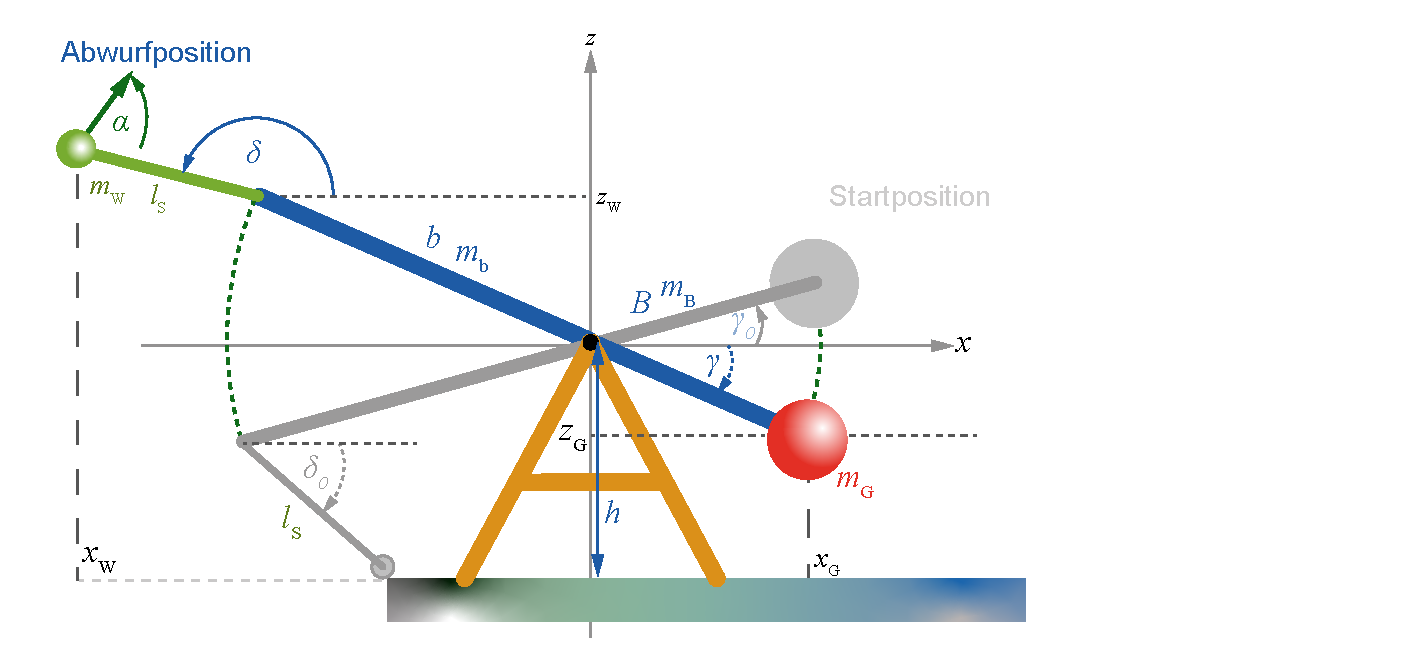
\includegraphics[width=\textwidth]{TrebNaeherung3.pdf}
\caption[Trebuchet mit Schleuder und fester Gegenmasse.]{Trebuchet mit Schleuder und fester Gegenmasse (Modell 3).}\label{abb:bew_TrebNaeherung3}
\end{figure}

Hier nehmen wir nun an, dass sich das Wurfgeschoss in einer Schleuder der L�nge $l_\text{W}$ befindet (\figref{bew_TrebNaeherung3}).
Dabei wird zugelassen, dass das Wurfgeschoss in seiner Beschleunigungsphase tiefer gelangen kann als es zum Zeitpunkt des Starts der Schleuder lag, wozu man im Mittelalter entsprechende Gr�ben aushub. 
Mit dieser Annahme unterliegt die Bewegung der Schleuder weiterhin keinen Zwangsbedingungen.
Als neue generalisierte Koordinate haben wir den Winkel $\delta$, der zum Startzeitpunkt so gew�hlt werden soll, dass die Schleuder gestrafft auf dem Boden liegt, \dh \[-\delta_0 = \arcsin\lk \frac{h-b\,\sin\gamma_0}{l_\text{W}}\rk\,. \]
Die Lagrange-Funktion f�r diesen Fall lautet 
	\begin{align}
		\mathcal{L}_{\uproman{3}} &= \mathcal{L}_{\uproman{1}} + \Delta\mathcal{L}_{\uproman{3}}  \nonumber \\
			& = \frac{J_0}{2}\,\dot{\gamma}^2 - f_0\,\sin\gamma + \ldots  \nonumber \\
			& ~~+ \frac{1}{2} J_\text{W}\,{\dot{\delta}}^2-J_\text{bW}\,\dot{\gamma}\,\dot{\delta}\,\cos\lk \gamma-\delta\rk - g\,m_\text{W}\,l_\text{W}\,\sin\delta\,, \label{eq:bew_treb09}
	\end{align}
woraus die Bewegungsgleichungen in Matrixform 
\begin{align}
		\mathbb{M}(t,\vec{q}) \cdot \ddot{\vec{q}}  
			& = 
\begin{pmatrix}
	J_0  ~~ & -J_\text{bW}\,\cos\lk \delta-\gamma \rk \\
			  -J_\text{bW}\,\cos\lk \delta-\gamma \rk ~~& J_\text{W}
\end{pmatrix}
\begin{bmatrix}
	\ddot{\gamma} \\
	\ddot{\delta} 
\end{bmatrix} \nonumber \\
	&= \begin{pmatrix}
	 -J_\text{bW}\,\dot{\beta}^2\,\sin\lk \beta-\gamma \rk - f_0\,\cos\gamma \\
	 +J_\text{bW}\,\dot{\gamma}^2\,\sin\lk \beta-\gamma \rk - g\,m_\text{W}\,l_\text{W}\,\cos\beta
\end{pmatrix} \nonumber \\
&= \vec{F}(t,\vec{q},\dot{\vec{q}}) \, \label{eq:bew_treb10}
\end{align}
folgen.
Auch hier integrieren wir die Bewegungsgleichungen numerisch
wie im vorherigen Abschnitt beschrieben und erkennen in
\figref{bew_TrebErgebnis3a} und Tabelle \ref{tab:bew_trebuchet_02}
ebenfalls eine deutliche Steigerung der Reichweite
und der Energieeffizienz gegen�ber der einfachen Steinschleuder. 
Diese resultieren aus der effektiven Verl�ngerung des Wurfarms durch die Schleuder, welche wiederum zu einer h�heren Abwurfgeschwindigkeit f�hrt.
Wir erkennen au�erdem, dass die maximale Reichweite weniger stark vom Ausl�sezeitpunkt abh�ngt.
Das bringt uns auf die Idee, die Modelle 2 und 3 zu kombinieren.

\begin{figure}
\begin{minipage}{\textwidth}
\leftfigure{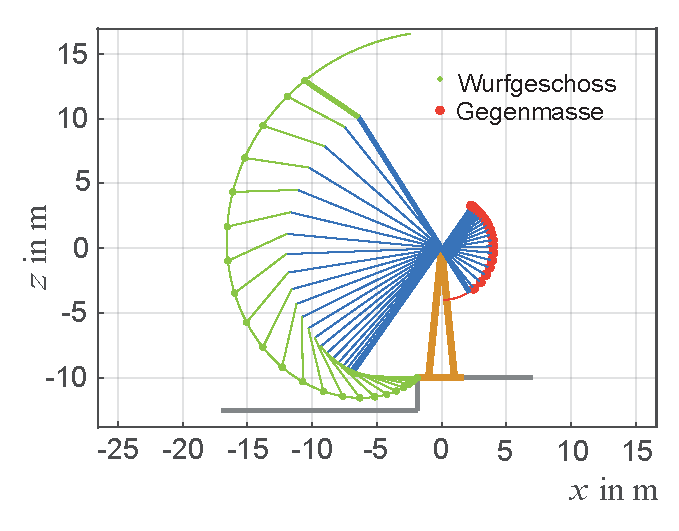
\includegraphics[width=0.5\textwidth]{TrebSim03b.pdf}}%
\hspace{\fill}
\rightfigure{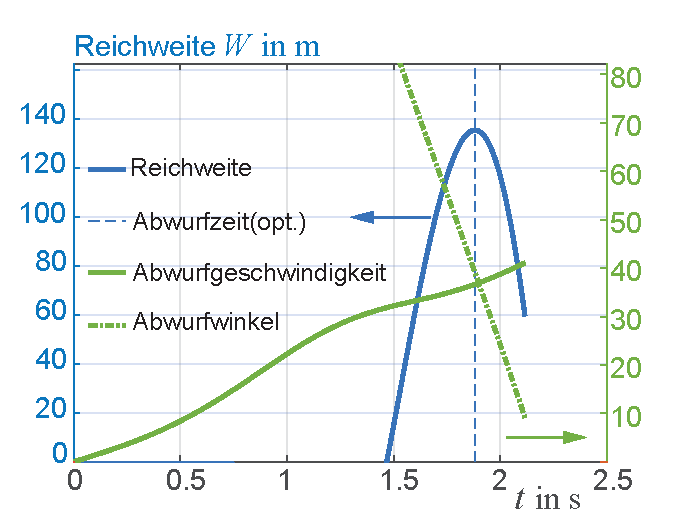
\includegraphics[width=0.5\textwidth]{TrebSim03a.pdf}}
\leftcaption[Dynamik eines Trebuchet mit Schleuder und fester Gegenmasse.]{Dynamik eines Trebuchet mit Schleuder und fester Gegenmasse (Modell 3).} \label{abb:bew_TrebErgebnis3b}
\rightcaption[Reichweite eines Trebuchet mit Schleuder und fester Gegenmasse.]{Reichweite eines Trebuchet mit Schleuder und fester Gegenmasse (Modell 3).} \label{abb:bew_TrebErgebnis3a}
\end{minipage}
\end{figure}

\subsubsection{Vollst�ndiges Trebuchet (Modell 4)} \label{kap:bew_trebuchet_complete}

Wir bringen nun alle Bauvarianten zusammen (\figref{bew_TrebNaeherung4}). 
Jetzt wollen wir auch ber�cksichtigen, dass zu Beginn der Bewegung die Schleuder mit dem Wurfgeschoss einer Zwangsbedingung unterliegt,
da sich das Wurfgeschoss in der Schleuder in der H�he $z_\text{W} = -h$ auf dem Boden bewegt, \dh es gilt die Zwangsbedingung \eqref{eq:bew_trebtheo01}:
		\begin{align}
				f\lk \gamma, \delta\rk = h -  b\,\sin\gamma + l_\text{W}\,\sin\delta = 0 \,. \label{eq:bew_treb11}
		\end{align}
Mit der Methode der Lagrange-Multiplikatoren (\kap{bew_Lagrange_I}) schreiben wir die Lagrange-Funktion als
		\begin{align}
		\begin{split}
				\mathcal{L}_{\uproman{4}} &=  \mathcal{L}_{\uproman{1}} + \Delta\mathcal{L}_{\uproman{2}} + \Delta\mathcal{L}_{\uproman{3}} + \ldots \\ 
				& ~~+ \frac{1}{2}J_0\,\dot{\gamma}^2 - f_0\,\sin\gamma  + \ldots \\
				& ~~+ \frac{1}{2}J_\text{G}{}^2\,\dot{\beta}^2 + J_\text{BG}\,\dot{\gamma}\,\dot{\beta}\,\cos\lk\gamma-\beta\rk - g\,m_\text{G}\,l_\text{G}\,\sin\beta
				+ \ldots \\
				& ~~+ \frac{1}{2}\,J_\text{W}\,\dot{\delta}^2 - J_\text{bW}\,\dot{\gamma}\,\dot{\delta}\,\cos\lk\gamma-\delta\rk - g\,m_\text{W}\,l_\text{W}\,\sin\delta + \ldots\\
				& ~~ + \lambda\lk h -  b\,\sin\gamma + l_\text{W}\,\sin\delta \rk \,.  \label{eq:bew_treb12}
		\end{split}
		\end{align}
Die Zwangskraft $\lambda$ h�lt das Wurfgeschoss auf der Bodenebene, sie ist $-m\,g$ beim Start des Trebuchet und wird Null beim \anf{Abheben}.
Zu diesem Zeitpunkt verliert auch die Zwangsbedingung ihre G�ltigkeit. 
Man muss also bei der numerischen Rechnung immer �berpr�fen, ob die Zwangsbedingung noch gilt.
Ebenso m�ssen die Anfangsbedingungen die Zwangsbedingung erf�llen.\\
Damit ergeben sich f�r $\gamma, \beta$, $\delta$ und $\lambda$ die folgenden drei Bewegungsgleichungen:
\begin{align}
	J_0\,\ddot{\gamma} 
		&= - m_\text{G}\,B\,l_\text{G}\,\ddot{\beta}\,\sin\lk \gamma+\beta\rk + m_\text{W}\,b\,l_\text{W}\,\ddot{\delta}\,\cos\lk\delta-\gamma\rk + \ldots  \nonumber \\
		&\quad + m_\text{G}\,B\,l_\text{G}\,\dot{\beta}^2\,\sin\lk\beta - \gamma\rk -m_\text{W}\,b\,l_\text{W}\,\dot{\delta}^2\,\sin\lk\delta-\gamma\rk - \ldots \nonumber  \\
		&\quad - f_0 \cos\gamma - \lambda\,b\,\cos\gamma \,, \\ \label{eq:bew_treb13}
	J_\text{G}\,\ddot{\beta}  &= -J_\text{BG}\,\ddot{\gamma}\cos\lk\beta-\gamma\rk - J_\text{BG}\dot{\gamma}^2\,\sin\lk\beta-\gamma\rk-g\,m_\text{G}\,l_\text{G}\,\cos\beta \,, \nonumber \\
	J_\text{W}\,\ddot{\delta} &= +J_\text{bW}\,\ddot{\gamma}\cos\lk\delta-\gamma\rk +J_\text{bW}\dot{\gamma}^2\,\sin\lk\delta-\gamma\rk-g\,m_\text{W}\,l_\text{W}\,l_\text{W}\,\cos\delta + \ldots \nonumber \\
		&\quad + \lambda\,\cos\delta \,.
\end{align}
Ferner ist die Zwangsbedingung \eqref{eq:bew_treb11} zu ber�cksichtigen. Wir k�nnten nun entsprechend der L�sungs--hinweise in \kapitel{bew_Lagrange_I} vorgehen.
Die analytische Berechnung wird aufgrund der Winkelfunktionsterme relativ un�bersichtlich und komplex, l�sst sich aber ohne weiteres in \matlab{} behandeln.
Wir wollen hier einen anderen Weg gehen, der sich an der Matrixstruktur der Bewegungsgleichungen \eqref{eq:bew_treb08} orientiert und daher besonders f�r die numerische Behandlung in \matlab{} geeignet ist.
Diese Methode l�sst sich verallgemeinern und kann insbesondere auch verwendet werden, wenn mehrere komplexe Zwangsbedingungen vorliegen und der oben beschriebene Ansatz an seine Grenzen kommt. 

Wir schreiben die Bewegungsgleichungen \eqref{eq:bew_treb13} wieder in Matrixform:
\begin{align}
			\mathbb{M}(\vec{q}) \cdot \ddot{\vec{q}} + \lambda \frac{\d f}{\d \vec{q}} = \vec{F}(\vec{q},\dot{\vec{q}})\,. \label{eq:bew_treb14}
\end{align}
Hierin ist
\begin{align}
\begin{split}
  \frac{\d f}{\d \vec{q}} &= \left[-b\,\cos\gamma~, ~0~,~l_\text{W}\,\cos\delta \right] \,,~~\vec{q} =[\gamma,\beta,\delta]^\text{T} \,,~~\\
	\dot{\vec{q}} &=[\dot\gamma,\dot\beta,\dot\delta]^\text{T} \,~~\text{und}~~\ddot{\vec{q}} =[\ddot{\gamma},~\ddot{\beta},~\ddot{\delta}]^\text{T} \,. 
\end{split} \label{eq:bew_treb14a}
\end{align}
Es sei betont, dass die Massen-Matrix $\mathbb{M}$ und der Kraftvektor $\vec{F}$ f�r das System ohne Zwangsbedingung aufgeschrieben wurden. 
\begin{align}
		\begin{split}
		\mathbb{M} = 
\begin{pmatrix}
	+J_0 & +J_\text{BG}\,\cos\lk\gamma-\beta\rk  & -J_\text{bW}\,\cos\lk\gamma-\delta\rk \\ \label{eq:bew_treb14b}
	+J_\text{BG}\,\cos\lk\gamma-\beta\rk   & +J_\text{G}  & 0\\
	-J_\text{bW}\,\cos\lk\gamma-\delta\rk   & 0   & +J_\text{W}
\end{pmatrix}\,.
\end{split}
\end{align}
Der Kraftvektor $\vec{F}$ ist gegeben durch
\begin{align}
\begin{split}
		\vec{F} = 
\begin{pmatrix}
	-J_\text{BG}\,{\dot{\beta}}^2\sin\lk\gamma-\beta\rk + J_\text{bW}\,{\dot{\delta}}^2\sin\lk\gamma-\delta\rk - f_0\,\cos\gamma \\
	+J_\text{BG}\,{\dot{\gamma}}^2\sin\lk\gamma-\beta\rk - m_\text{G}\,l_\text{G}\,g\,\cos\beta \\ \label{eq:bew_treb14c}
	-J_\text{bW}\,{\dot{\delta}}^2\sin\lk\gamma-\delta\rk - m_\text{W}\,l_\text{W}\,g\,\cos\delta
\end{pmatrix}\,.
\end{split}
\end{align}
Da die Zwangsbedingung in unserem Fall nicht explizit von der Zeit abh�ngt, gilt
\begin{align*}
		\frac{\D f}{\D t} = 0 = \frac{\d f}{\d \vec{q}} \cdot \dot{\vec{q}} \,, 
\end{align*}
woraus f�r die zweite Ableitung sofort folgt:
\begin{align}
		\frac{\D^2 f}{\D\,t^2} &= 0 = \frac{\d }{\d \vec{q}} \lk \frac{\d f}{\d \vec{q}} \cdot \dot{\vec{q}} \rk \cdot \dot{\vec{q}} + \frac{\d f}{\d \vec{q}} \cdot \ddot{\vec{q}} \quad
		\rightarrow \quad \frac{\d f}{\d \vec{q}} \cdot \ddot{\vec{q}} = -\frac{\d }{\d \vec{q}} \lk \frac{\d f}{\d \vec{q}} \cdot \dot{\vec{q}} \rk \cdot \dot{\vec{q}} = F_{\lambda} \,. \label{eq:bew_treb15}
\end{align}
In unserem Fall%
\footnote{$F_\lambda$ ist, wenn wir die Zwangsbedingung in der Dimension L�nge aufschreiben,
unabh�ngig von der Wahl der generalisierten Koordinaten eine Beschleunigung.
Wir behalten aber die Bezeichnung $F_\lambda$ bei, da ja $\lambda$
die Bedeutung einer verallgemeinerten Zwangskraft hat (siehe \kap{bew_Lagrange_I}.)}
ist
\begin{align}
	F_{\lambda} = -b\,{\dot{\gamma}}^2\,\sin\gamma\,+\,l_\text{W}\,{\dot{\delta}}^2\,\sin\delta \,.\label{eq:bew_treb16}
\end{align}
Damit k�nnen wir nun die Bewegungsgleichung kompakt in Matrixform schreiben: 
\begin{align}
		\begin{split}
		\underbrace{\lk \begin{array} {cc}
				\mathbb{M} ~~ & ~\lek \frac{\d f}{\d \vec{q}}\rek^\text{T}\\  \frac{\d f}{\d \vec{q}} ~~& ~ 0 
		\end{array} \rk }_{\hat{\mathbb{M}}} \cdot 
		\underbrace{\lek \begin{array} {l}
				\ddot{\vec{q}}\\
				\lambda 
		\end{array} \rek}_{\ddot{\vec{Q}}} &= 
		\underbrace{\lek \begin{array} {l}
				\hat{\vec{F}}\\
				F_\lambda 
		\end{array} \rek }_{\vec{F}_\text{ZB}} \,. \label{eq:bew_treb17}
		\end{split}
\end{align}

Mit \eqref{eq:bew_treb17} haben wir ein Gleichungssystem mit vier Gleichungen f�r vier Unbekannte, das wir jetzt noch f�r die Berechnungen in \matlab{} in eine passende Form bringen m�ssen. 
Wir erinnern uns, dass die Gleichungen f�r die zweiten Ableitungen $\ddot{q}_i$ durch je zwei Gleichungen ersetzt werden m�ssen, indem wir $Y_1 = q_1$ und $Y_2 = \dot{q}_1$ setzen.
Entsprechend m�ssen wir die Matrix $\mathbb{M}$ zu $\hat{\mathbb{M}}$ und die Vektoren $\ddot{\vec{Q}},~\vec{F}$ zu $\dot{\vec{Y}},~\hat{\vec{F}}$ erweitern.
Wir erhalten
\begin{align}
		\begin{split}
		\hat{\mathbb{M}} = 
		\lk \begin{array} {lllllll}
				 1 ~~~~& 0 & 0 ~~~~ & 0 & 0 ~~~& 0 & 0 ~~~~ \\
				 0 & M_{11} ~~& 0 & M_{12}~~ & 0 & M_{13}~~ & f_\text{Y1} \\
				 0 & 0 & 1 & 0 & 0 & 0 & 0  \\
				 0 & M_{21} ~~& 0 & M_{22}~~ & 0 & M_{23}~~ & f_\text{Y5} \\
				 0 & 0 & 0 & 0 & 1 & 0 & 0  \\
				 0 & M_{31} ~~& 0 & M_{32}~~ & 0 & M_{33}~~ & f_\text{Y5} \\
				 0 & f_\text{Y1} ~~& 0 & f_\text{Y3}~~ & 0 & f_\text{Y5}~~ & 0 \,
		\end{array} \rk \,, \: \dot{\vec{Y}}=
		\lek \begin{array} {l}
				\dot{Y}_1 = \dot{\gamma}\\
				\dot{Y}_2 = \ddot{\gamma}\\
				\dot{Y}_3 = \dot{\beta}\\
				\dot{Y}_4 = \ddot{\beta}\\
				\dot{Y}_5 = \dot{\delta}\\
				\dot{Y}_6 = \ddot{\delta}\\
				\dot{Y}_7 = \dot\lambda\\
		\end{array} \rek \,, \: \vec{\hat{\vec{F}}}= 
		\lek \begin{array} {l}
				A_1 = Y_1\\
				A_2 = F_1\\
				A_3 = Y_2\\
				A_4 = F_2\\
				A_5 = Y_3\\
				A_6 = F_3\\
				A_7 = F_\lambda
		\end{array} \rek\,.
		\end{split} \label{eq:bew_treb17a}
\end{align}
Hier ist
	\[\lek f_\text{Y1}, f_\text{Y3}, f_\text{Y5} \rek^\text{T} = \frac{\d f}{\d \vec{q}} = \lek  \frac{\d f}{\d \gamma},  \frac{\d f}{\d \beta}, \frac{\d f}{\d \delta} \rek^\text{T} = \lek -b\,\cos\gamma,~0~,~l_\text{W}\,\cos\delta \rek^\text{T} \,.
	\]
Bei genauer Betrachtung von \eqref{eq:bew_treb17a} sieht man, dass es sich nicht um ein gew�hnliches DGL-System handelt\index{Differentialgleichungssystem}, sondern um ein sogenanntes \emph{Differential-Algebraisches (DAE) System}\index{Differential-Algebraisches System}, denn die Matrix $\mathbb{M_\text{ZB}}$ ist singul�r, da zu ihr keine inverse Matrix existiert \cite{Pietruszka2020}. 
Die L�sung eines solchen DAE-Systems erfolgt daher mit dem \odeefs-Solver von \matlab{} (siehe Anhang in den \onlineZ{} und \mscr{} \mlbewref{TrebSimDAE.m}), wobei die Massen-Matrix in der um $\d f/\d \vec{q}$ erweiterten Form $\mathbb{M}$ \eqref{eq:bew_treb17a} an die \matlab-Routine \odeefs{} �bergeben werden muss. \\
Man muss bei der Berechnung der Zeitentwicklung der generalisierten Koordinaten immer �berpr�fen,
ob die Zwangsbedingung $f \lk q(t) \rk = 0$ noch gilt, \dh ob das System noch in Phase 1 ist.
Sobald der Zeitpunkt $t_1$ erreicht ist, berechnet man die Dynamik einfach
nach \eqref{eq:bew_treb14} mit $\lambda \equiv 0$ und benutzt die \odevf-Routine von \matlab.
Das Ergebnis ist in den \figref{bew_TrebErgebnis4a} und \figref{bew_TrebErgebnis4b} gezeigt,
sowie in Tabelle \ref{tab:bew_trebuchet_02} und Tabelle \ref{tab:bew_trebuchet_03} . 
Interessanterweise ist beim vollst�ndigen Trebuchet die erzielbare Reichweite
etwas geringer als die Reichweite der Modelle 2 und 3.
Daf�r ist der Zeitbereich f�r das Ausl�sen des Trebuchet gr��er geworden
und damit die Konstruktion des Ausl�semechanismus einfacher.
Durch entsprechende Variation der Parameter $b$, $B$ und $l_\text{W}$
und unter Beibehaltung der Bauh�he $h$, der Balkenl�nge $L_\text{T} = B+b$
und der Massen $m_\text{G}$, $m_\text{T}$, sowie $m_\text{W}$
kann die Reichweite optimiert werden (Tab. \ref{tab:bew_trebuchet_03}).
Die errechneten Werte sind beeindruckend und stimmen auch gut
mit den historischen Beschreibungen �berein. 
Wer m�chte, kann noch die Reibung, sowohl am Trebuchet als auch in der Flugphase, ber�cksichtigen.
Diese f�hrt nat�rlich zu etwas geringeren Reichweiten.
Ebenso kann man bei Ber�cksichtigung der Reibung im Lager
die \anf{Relaxationsdynamik} des Trebuchet nach dem Abwurf berechnen.
Wenn man ber�cksichtigt, dass die Waffenmeister des Mittelalters diese Trebuchet
nur aus ihren Erfahrungen heraus und ohne jegliche Kenntnis des Lagrange-Formalismus
gebaut haben, ist man schon schwer beeindruckt.


\begin{figure}
\begin{minipage}{\textwidth}
\leftfigure{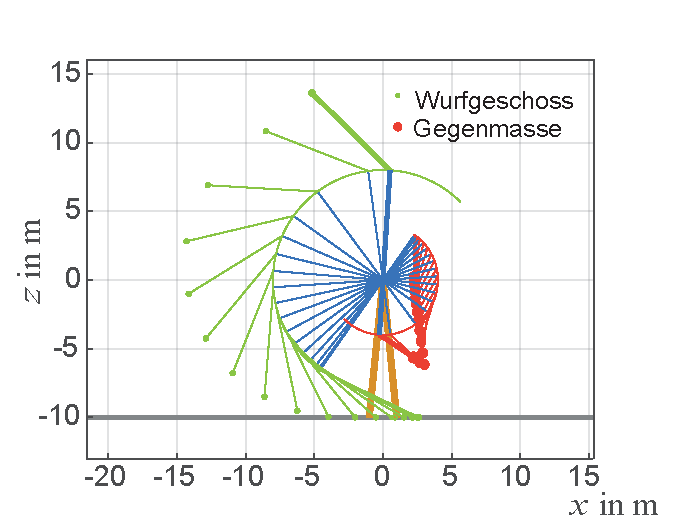
\includegraphics[width=0.5\textwidth]{TrebSim04b.pdf}}%
\hspace{\fill}
\rightfigure{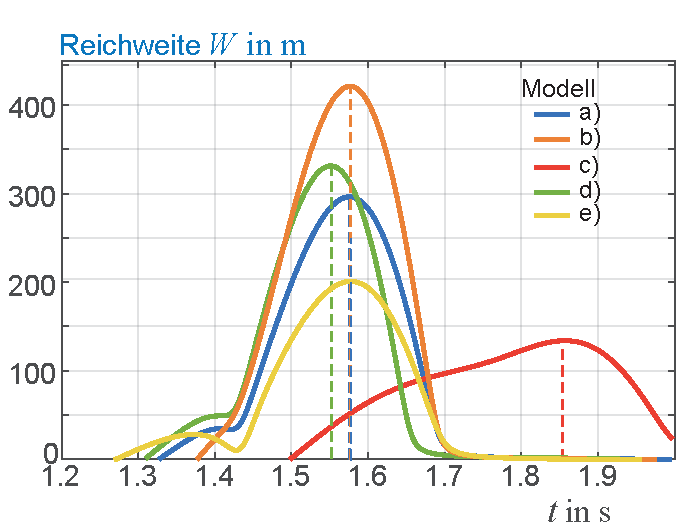
\includegraphics[width=0.5\textwidth]{TrebSim04a.pdf}}
\leftcaption[Dynamik eines Trebuchet unter Ber�cksichtigung einer Zwangsbedingung.]{Dynamik eines Trebuchet unter Ber�cksichtigung einer Zwangsbedingung.} \label{abb:bew_TrebErgebnis4b}
\rightcaption[Reichweite f�nf verschiedener Trebuchet.]{Reichweite f�nf verschiedener Trebuchet. Parameter siehe Tabelle \ref{tab:bew_trebuchet_03}.}
\label{abb:bew_TrebErgebnis4a}  
\end{minipage}
\end{figure}


\begin{table}
  \centering
  \begin{tabular}{|c|r|r|r|r|r@.l|r@.l|r@.l|r@.l|r@.l|r@.l|}
%  \begin{tabular}{|c|r|r|r|r|rl|rl|rl|rl|rl|rl|}
  \hline
  %\rule{0pt}{3pt}\\
  \phantom{x}&\phantom{x}&\phantom{x}&\phantom{x}&\phantom{x}&\multicolumn2{c|}{\phantom{x}}&\multicolumn2{c|}{\phantom{x}}&\multicolumn2{c|}{\phantom{x}}&\multicolumn2{c|}{\phantom{x}}&\multicolumn2{c|}{\phantom{x}}&\multicolumn2{c|}{\phantom{x}}\\
  Parameter & $l_\text{G}  $ & $l_\text{W}  $ & $B  $ & $b  $ & \multicolumn2{c|}{$ W  $} & \multicolumn2{c|}{$t_\text{abw} $}   & \multicolumn2{c|}{$\alpha   $} & \multicolumn2{c|}{$v_\text{abw}    $} & \multicolumn2{c|}{$\epsilon_\text{W}    $} & \multicolumn2{c|}{$\epsilon_\text{T}    $} \\
  Einheit   & $\si{\metre}$ & $\si{\metre}$ & $\si{\metre}$ &  $\si{\metre}$ & \multicolumn2{c|}{$ \si{\metre}$} & \multicolumn2{c|}{$\si{\second}$} & \multicolumn2{c|}{$ \si{\degree}$} & \multicolumn2{c|}{$\si{\metre\per\second} $} & \multicolumn2{c|}{$\si{\%}$} & \multicolumn2{c|}{$\si{\%}$} \\
  \phantom{x}&\phantom{x}&\phantom{x}&\phantom{x}&\phantom{x}&\multicolumn2{c|}{\phantom{x}}&\multicolumn2{c|}{\phantom{x}}&\multicolumn2{c|}{\phantom{x}}&\multicolumn2{c|}{\phantom{x}}&\multicolumn2{c|}{\phantom{x}}&\multicolumn2{c|}{\phantom{x}}\\
  %\rule{0pt}{3pt}\\
  \hline
  Fall   a) &          3 &          8 &          4 &           8 & 296&2 & 1&58 & 35&1 & 55&4 & 18&2 & 19&6 \\
  Fall   b) &          3 & \textbf{9} & \textbf{3} &  \textbf{9} & 427&0 & 1&60 & 34&8 & 66&7 & 38&0 & 41&5 \\
  Fall   c) &          3 &          8 & \textbf{2} & \textbf{10} & 133&1 & 1&86 & 26&4 & 40&2 & 20&9 & 27&3 \\
  Fall   d) & \textbf{4} &          8 &          4 &           8 & 327&2 & 1&57 & 33&9 & 58&8 & 20&7 & 22&7 \\
  Fall   e) &          3 & \textbf{7} &          4 &           8 & 198&5 & 1&58 & 32&3 & 46&3 & 12&1 & 13&6 \\
  \hline
  \end{tabular}
\medskip
\caption[Reichweiten und Effizienzparameter f�r verschiedene Trebuchet-Designs. Die Zwangsbedingung ist ber�cksichtigt.]{Reichweiten und Effizienzparameter f�r verschiedene Trebuchet-Designs. Die Zwangsbedingung ist ber�cksichtigt. Weitere Parameter: $h= \SI{10}{\metre}$, $m_\text{G} = \SI{10000}{\kilogram}$, $m_\text{W} = \SI{100}{\kilogram}$, $m_\text{T} = \SI{1040}{\kilogram}$. Die Berechnungen finden sich in den einzelnen \mscr en.} \label{tab:bew_trebuchet_03}
\end{table}

Zum Schluss geben wir noch die Erweiterung von \eqref{eq:bew_treb17} auf mehrere Zwangsbedingungen an.
Man erh�lt nach einfacher �berlegung
\begin{align}
		\begin{split}
		\lk \begin{array} {cc}
				\mathbb{M} ~~ & ~ \lek \frac{\d \vec{f}}{\d \vec{q}}\rek^\text{T}\\
				\frac{\d \vec{f}}{\d \vec{q}} ~~& ~ \vec{0} 
		\end{array} \rk \cdot 
		\lek \begin{array} {l}
				\ddot{\vec{q}}\\
				\vec{\lambda}
		\end{array} \rek &= 
		\lek \begin{array} {l}
				\vec{F}\\
				\vec{F}_\lambda
		\end{array} \rek \,, \label{eq:bew_treb17b}
		\end{split}
\end{align}
worin $\vec{\lambda} = (\lambda_1, \lambda_2, \ldots)$, $\vec{F}_\lambda = (F_{\lambda 1}, F_{\lambda 2}, \ldots)$ und $\d \vec{f}/\d \vec{q}$ die \emph{Jacobi}\indexp{Jacobi, Carl Gustav Jacob}\index{Jacobi-Matrix|textbf}\emph{-Matrix} ist (siehe Infokasten) und \cite{Andrews2003, Riley2006, Bartelmann2015}.\\
%\footnote{Carl Gustav Jacob Jacobi (1804--1851) war einer deutscher Mathematiker, der zu den produktivsten und vielseitigsten Mathematikern z�hlt.
%Besonders seine Theorie der elliptischen Funktionen, aber auch seine Arbeiten zur Differentialgeometrie waren f�r die mathematischen Physik wegbereitend.
%Die Hamilton-Jacobi-Theorie der klassischen Mechanik war eine wichtige Vorstufe f�r den sp�teren �bergang zur Quantenmechanik.}
\medskip
\fbox{\parbox{1.0\textwidth}{
\medskip
\textbf{\textit{Jacobi-Matrix}}\\
Die Jacobi-Matrix\indexp{Jacobi,Carl Gustav Jacob} wird auch Funktionalmatrix oder Ableitungsmatrix genannt) und ist eine $m \times n$\,-Matrix s�mtlicher erster partieller Ableitungen der $i=1 \ldots m$\, Komponenten einer Funktion $\vec{f}$ (also der $f_m$) nach den $j = 1 \ldots n$\, Variablen:
\begin{align}
\mathbb{J} =  \frac{\d f_j}{\d q_i} =
\begin{pmatrix}
  \frac{\d f_1}{\d q_1} & \frac{\d f_2}{\d q_1}& 
    \ldots & 
    \frac{\d f_{m-1}}{\d q_1} &\frac{\d f_m}{\d q_1} \\[2ex] % <-- 1ex more space between rows of matrix
  \frac{\d f_2}{\d q_1} & \frac{\d f_2}{\d q_2}&
    \ldots & 
    \frac{\d f_{m-1}}{\d q_2} &\frac{\d f_m}{\d q_2} \\[2ex] % <-- 1ex more space between rows of matrix
  \vdots&  & & & \vdots \\[2ex]
  \frac{\d f_1}{\d q_{n-1}} & \frac{\d f_2}{\d q_{n-1}}& 
    \ldots & 
    \frac{\d f_{m-1}}{\d q_{n-1}} &\frac{\d f_m}{\d q_{n-1}}\\[2ex]%
  \frac{\d f_1}{\d q_n} & \frac{\d f_2}{\d q_n} &
    \ldots & 
    \frac{\d f_{m-1}}{\d q_n} &\frac{\d f_m}{\d q_n} 
\end{pmatrix} \,. \label{eq:bew_Jacobi_function01}
\end{align} 
%\begin{align}
%\mathbb{J} = J_{i,j} =
%\begin{pmatrix}
  %\frac{\d f_1}{\d q_1} & 
    %\frac{\d f_1}{\d q_2} & 
    %\frac{\d f_1}{\d q_3} \\[1ex] % <-- 1ex more space between rows of matrix
  %\frac{\d f_2}{\d q_1} & 
    %\frac{\d f_2}{\d q_2} & 
    %\frac{\d f_2}{\d q_3} \\[1ex]
  %\frac{\d f_3}{\d q_1} & 
    %\frac{\d f_3}{\d q_2} & 
    %\frac{\d f_3}{\d q_3} 
%\end{pmatrix} \,. \label{eq:bew_Jacobi_function01}
%\end{align} 
Die Jacobi-Matrix findet weitreichende Anwendungen bei der Approximation und Extremwertberechnung mehrdimensionaler Funktionen und besonders auch bei Koordinatentransformationen.
So hat \zb die Jacobi-Matrix f�r die Koordinatentransformation von kartesischen $f_j =(x,y,z)$ in sph�rische $q_i =(r,\vartheta,\varphi)$ Koordinaten mit $i,j = 1 \ldots 3$ die folgende Form:
\begin{align}
\mathbb{J} = \frac{\d f_j}{\d q_i} = \begin{pmatrix} \sin\vartheta \cos\varphi & ~~r \cos\vartheta\cos\varphi &~~ -r \sin\vartheta\sin\varphi\\ \sin\vartheta \cos\varphi &~~ r \cos\vartheta\sin\varphi &~~ r \sin\vartheta\cos\varphi\\ \cos\vartheta &~~- r \sin\vartheta &~~ 0 \end{pmatrix} \,. \label{eq:bew_Jacobi_function02}
\end{align}
Da in diesem Fall die Jacobi-Matrix eine quadratische Matrix ist, l�sst sich deren Determinante berechnen. Diese wird Jacobi-Determinante genannt. Sie spielt bei der Koordinatentransformation von Integralen eine wichtige Rolle und die Berechnung des Volumenelements ergibt im vorliegenden Fall: 
%\begin{align}
 %\det\,\mathbb{J}(r,\vartheta,\varphi) = r^2\,\sin\vartheta\,. \label{eq:bew_Jacobi_function03}
%\end{align}
\begin{align}
 \D V = \D x \, \D y \, \D z \, =  \det \,\mathbb{J} \:\, \D r\,\D \vartheta\,\D \varphi = r^2\sin\vartheta\,\D r\,\D \vartheta\,\D \varphi\,. \label{eq:bew_Jacobi_function04}
\end{align}
}}

Ein Beispiel f�r ein Trebuchet mit mehreren Zwangsbedingungen ist in \probref{bew_Trebuchet_II} gegeben, die auf einer Arbeit von \cite{Constans2017} beruht.
Wir werden bei der L�sung bis zu vier Zwangsbedingungen bei f�nf generalisierten Koordinaten verarbeiten, so dass die Jacobi-Matrix $\d \vec{f}/\d \vec{q}$ die Dimension~$5\times4$ annehmen kann.\\
Wir haben mit diesem sch�nen und illustrativen Beispiel des Trebuchet noch einmal gezeigt, dass man mit dem Lagrange-Formalismus f�r Massepunkte recht komplexe Systeme sehr effizient beschreiben und numerisch behandeln kann.


\clearpage
%\clearpage
%\section{Tabellen}\label{kap:bew_tabellen}

\clearpage



\renewcommand\glslongextraNameAlign{p{36mm}}
\renewcommand\glslongextraDescAlign{p{60mm}}
\clearpage
\bgroup
\small
\printunsrtglossary[type=bew]
\egroup
\clearpage
\fancyhead[RE]{\nouppercase\rightmark}
\begingroup
\let\cleardoublepage\relax
\bibliography{referenzen}
\endgroup
\fancyhead[RE]{\nouppercase\leftmark}
%%%%%%%%%%%%%%%%%%%%%%%%%%%%%%%%%%%%%%%%%%%%%%%%%%%%%%%%%%%%%
%\input{footer.tex}
